\documentclass[11pt]{book}
\usepackage{sfx_package}
\usepackage{lscape}
\usepackage{textcomp}
%%%%%%%%%%%%%%%%%%%%%%%%%%%%%%%%%%%%%%%%%%%%%%%%%%%%%%%%%%%%%%%%
\usepackage{multicol}
\usepackage{multirow}
\usepackage{fancyhdr}
\usepackage{colordvi}
\usepackage{graphicx}
\usepackage{supertabular}
%
%\usepackage{amsmath,amssymb,float}
%AAB to be able to use certain amsmath features
\usepackage{amsmath}
%AAB to be able to use \mathsrc font:
\usepackage{mathrsfs}
%
\usepackage{afterpage}
\usepackage{float}
\usepackage{subfigure}
\usepackage{color}
%====================
\bibliographystyle{plain}
\usepackage[sectionbib]{chapterbib}
%====================
%numerotation des ligne pour relecture
%\usepackage[left,modulo]{lineno}
%\linenumbers
%\usepackage{url}
%\usepackage{apalike}
%%%%%%%%%%%%%%%%%%%%%%%%%%%%%%%%%%%%%%%%%%%%%%%%%%%%%%%%%%%%%%%%
%\newcommand{\etal}{{et al.\ }}
\newcommand{\eg}{{e.g.\ }}
\newcommand{\ie}{{i.e.\ }}
\newcommand{\para}{ }
\newcommand{\pa}{\\}
\newcommand{\tabline}{\hline}
%\newcommand{\cta}[2]{{\it{#1}}~(#2)}
\newcommand{\cta}[2]{#1~(#2)}
\newcommand{\ctb}[2]{({\it{#1}}~(#2))}
\newcommand{\ctc}[4]{({\it{#1}}~(#2),~{\it{#3}}~(#4))}
\newcommand{\ctd}[6]{({\it{#1}}~(#2),~{\it{#3}}~(#4),~{\it{#5}}~(#6))}
\newcommand{\cte}[8]{({\it{#1}}~(#2),~{\it{#3}}~(#4),~{\it{#5}}~(#6),~{\it{#7}}~(#8))}
%%%%%%%%%%%%%%%%%%%%%%%%%%%%%%%%%%%%%%%%%%%%%%%%%%%%%%%%%%%%%%%%
\renewcommand{\baselinestretch}{1.1}
%%%%%%%%%%%%%%%%%%%%%%%%%%%%%%%%%%%%%%%%%%%%%%%%%%%%%%%%%%%%%%%%

%\DeclareUnicodeCharacter{2212}{*************************************}

\begin{document}
\title{SURFEX SCIENTIFIC\\ DOCUMENTATION}
\author{P. Le Moigne}
%\date{March 17, 2009}
\maketitle
%\dominitoc

%---------------------------------
{\large{~ \\ \\ \\ 
EDITOR :  Patrick Le Moigne \\ \\

Contributing authors :  \\ \\

%v8.1
2018\\
C.~Albergel       $^{(1)}$, 
A.~Boone          $^{(1)}$, 
S.~Belamari       $^{(1)}$, 
%expected contribution D.~Carrer         $^{(1)}$, 
B.~Decharme       $^{(1)}$,  
%expected contribution C.~Delire         $^{(1)}$, 
M.~Dumont         $^{(4)}$, \\ 
%expected contribution C.~Lebeaupin      $^{(2)}$,  
P.~Le~Moigne      $^{(1)}$, 
V.~Masson         $^{(1)}$  \\ \\ \\
%expected contribution D.~Salas~y~Melia  $^{(1)}$  \\ \\ \\ 

%v7.2
2012\\
A.~Boone          $^{(1)}$, 
S.~Belamari       $^{(1)}$, 
E.~Brun           $^{(1)}$, 
J.-C.~Calvet      $^{(1)}$, 
B.~Decharme       $^{(1)}$,  
H.~Giordani       $^{(1)}$,  \\
S.~Lafont         $^{(1)}$,  
P.~Le~Moigne      $^{(1)}$, 
S.~Morin          $^{(4)}$, 
V.~Vionnet        $^{(1)}$  \\ \\ \\

% v5 :
2009\\
A.~Boone          $^{(1)}$, 
J.-C.~Calvet      $^{(1)}$, 
B.~Decharme       $^{(1)}$, 
S.~Faroux         $^{(1)}$, 
A.-L.~Gibelin     $^{(1)}$, 
C.~Lebeaupin      $^{(2)}$,  \\
P.~Le~Moigne      $^{(1)}$, 
J.-F.~Mahfouf     $^{(1)}$, 
E.~Martin         $^{(1)}$, 
V.~Masson         $^{(1)}$, 
D.~Mironov        $^{(3)}$, 
J.~Noilhan        $^{(1)}$, \\
P.~Tulet          $^{(1)}$,
B.~Van~Den~Hurk   $^{(4)}$  \\ \\ \\ 


$^{(1)}$ : CNRM-UMR3589, M\'et\'eo-France/CNRS, Toulouse, France \\ 
$^{(2)}$ : Laboratoire de M\'et\'eorologique Dynamique, Ecole Polytechnique, Palaiseau, France \\ 
$^{(3)}$ : German Weather Service, Offenbach am Main, Germany  \\ 
$^{(4)}$ : CNRM-UMR3589, M\'et\'eo-France/CNRS, Grenoble, France \\ 
$^{(5)}$ : KNMI, The Netherlands

~\\ \\ \\ \\ \\ \\ 

{\it{Dissemination Level :}} public


}}

%---------------------------------
%---------------------------------
%  DESCRIPTION DES CHANGEMENTS
%---------------------------------
%---------------------------------
\newpage
\begin{tabular}{|c|c|c|c|c|}
\hline
ISSUE No       &   &      DATE           &      PAGES      &         DESCRIPTION OF CHANGE                        \\
\hline
   1           & V5.0  &      May 2009       &      1 - 211    &         Original                                 \\
\hline
   2           & V7.2  &      March 2012     &      1 - 235    &         Description of Crocus, Isba-CC, Teb-Veg  \\
               &       &                     &                 &         Bibliography references by chapter       \\
               &       &                     &                 &                                                  \\
\hline
   3           & V8.0  &      February 2018  &      1 - 304    &         Description of MEB, TARTES,              \\
               & and   &                     &                 &         Revision of ISBA-ES, ISBA-DF             \\
               & V8.1  &                     &                 &         Revision of TEB+VEG                      \\
               &       &                     &                 &         Revision of water surfaces               \\
\hline
\end{tabular}
\newpage
%---------------------------------
%---------------------------------
%---------------------------------
%---------------------------------
\dominitoc
\tableofcontents

\part{SURFACE PROCESSES SCHEME}
%%%%%%%%%%%%%%%%%%%%%%%%%%%%%%%%%%%%%%%%%%%%%%%%%%%%%%%%%%%%%%%%%%%%%%%%%%%%%%%
% CONTRIBUTION TO THE SURFEX BOOK1: "Surface Processes Scheme"
% Author        : P. Le Moigne
% Original      : January 05, 2009
% Last Update   : January 05, 2009
% Last Update   : May     06, 2009
%%%%%%%%%%%%%%%%%%%%%%%%%%%%%%%%%%%%%%%%%%%%%%%%%%%%%%%%%%%%%%%%%%%%%%%%%%%%%%%

\chapter{Introduction: a brief description of the SURFEX system}
\minitoc
%=========================
\bibliographystyle{plain}
%=========================

%{by P. Le Moigne}

Surface modelling in numerical weather prediction has always held an important place in the activities of the Centre National de Recherches M\'et\'eorologiques (CNRM hereafter). In the late 80's, Isba (Noilhan and Planton~(1989)\nocite{Noilhan1989}; Mahfouf and Noilhan~(1996)\nocite{Mahfouf1996}), a soil vegetation atmosphere transfer scheme (Interaction between Soil Biosphere and Atmosphere) has been developed and it aimed to better simulate the exchanges of energy and water between the land surface and the atmosphere just above. Isba model has been designed to be simple and efficient in order to be put into operations at M\'et\'eo-France. Isba scheme computes the exchanges of energy and water between  the continuum soil-vegetation-snow and the atmosphere above. In its genuine version, the evapotranspiration of the vegetation is controlled by a  resistance like proposed by Jarvis (1976)\nocite{Jarvis1976}
. A more recent version of the model named Isba-A-gs (Calvet \etal (1998)\nocite{Calvet1998})
 accounts for a simplified photosynthesis model where the evaporation is controlled by the aperture of the stomates, the component of the leaves that regulates the balance between the transpiration and the assimilation of CO2. Nowadays, Isba land surface scheme is used in the French operational and research forecast models. Thanks to the efforts made by the research community at CNRM, French numerical weather prediction models have always been at the forefront of research in terms of surface modelling. More recently, the modelling of urban areas has began to be of great interest in the research community. In 2000, TEB (Town Energy Balance) model, specially designed to represent the exchanges between a town and the atmosphere has enabled advanced studies in this direction (Masson (2000)\nocite{Masson2000}). The TEB model is based on the canyon concept, where a town is represented with a roof, a road and two facing walls with characteristics playing a key role in the town energy budget. More especially, the ability, of the canyon to trap a fraction of the incoming solar and infrared radiation is taken into account in the model.
A special effort has been made this last years to externalize the surface scheme from the embedded surface-atmosphere Meso-NH model. The main idea was to gather all the developments and improvements made in surface schemes in order to make them available for as many people as possible. Not only physical parameterizations have been externalized, but also the preparation of specific surface parameters needed by physical schemes and the initialization of all state variables of the different models: SURFEX (stands for surface externalis\'{e}e) system was born. 
Moreover, the surface representation has been improved and thus Surfex system has been enhanced with the specific treatment for water surfaces. Indeed, up to now, the exchanges of energy between water surfaces and the atmosphere were treated in a very simple way, while now a physically based model have been introduced to build a more complex but accurate surface model, available for all atmospheric models. There are two possibilities to compute fluxes over marine surfaces. The simplest one consists in using Charnock's approach to compute the roughness length and fluxes with a constant water surface temperature. Secondly, a one-dimensional ocean mixing layer model has been introduced (Lebeaupin (2007)\nocite{lebeaupin2007})
 in order to simulate more accurately the sea surface temperature (SST hereafter) and the fluxes at the sea/air interface. This model based on Gaspar (1990)\nocite{Gaspar1990}
, will be very helpful especially at meso-scale to better represent diurnal cycle of SST. 
At meso-scale, a good representation of lakes is of great interest especially for Northern countries. In order to  improve the treatment of lake areas, the simple but robust Flake model (Mironov (2010)\nocite{mironov2010}) has been implemented within Surfex system. It allows to have an evolving lake surface temperature and a good description of the energy exchanges within water.

\begin{figure}[h]
\hspace*{2.cm}
\psfig{figure=\EPSDIR/dessin-3.eps2,width=12cm}
\caption{ Description of the exchanges between an atmospheric model sending meteorological and radiative fields to the surface and Surfex composed of a set of physical models that compute tiled variables $\mathcal{F}_{*}$ covering a fraction f$_{*}$ of a unitary grid box and an interface where the averaged variables $\mathcal{F}$ are sent back to the atmosphere \label{surf1}}
\end{figure}

%\begin{figure}[h]
%\hspace*{2.cm}
%\psfig{figure=\EPSDIR/4flux.eps,width=12cm}
%\caption{Partitioning of the SURFEX grid box, and corresponding turbulent fluxes.
%F stands either for M (momentum flux), H (sensible heat flux), LE (latent heat flux),
%$S^\uparrow$ (the reflected solar radiation) or $L^\uparrow$ (the
%upward longwave radiation).
%\label{surf1}}
%\end{figure}

%\begin{displaymath}
%\begin{array}{lclclclcl}
%M &= & M_{sea} & + & M_{water} & + & M_{town} & + & M_{nature} \\
%H &= & H_{sea} & + & H_{water} & + & H_{town} & + & H_{nature} \\
%LE &= & LE_{sea} & + & LE_{water} & + & LE_{town} & + & LE_{nature} \\
%S^\uparrow &= & S^\uparrow_{sea} & + & S^\uparrow_{water} & + & S^\uparrow_{town} & + & S^\uparrow_{nature} \\
%L^\uparrow &= & L^\uparrow_{sea} & + & L^\uparrow_{water} & + & L^\uparrow_{town} & + & L^\uparrow_{nature} \\
%\end{array}
%\end{displaymath}

In Surfex, the exchanges between the surface and the atmosphere are realized by mean of a standardized interface (Polcher \etal (1998)\nocite{Polcher1998}; Best \etal (2004)\nocite{Best2004}) that proposes a generalized coupling between the atmosphere and surface. During a model time step, each surface grid box receives the upper air temperature, specific humidity, horizontal wind components, pressure, total precipitation, long-wave radiation, short-wave direct and diffuse radiations and possibly concentrations of chemical species and dust. In return, Surfex computes averaged fluxes for momentum, sensible and latent heat and possibly chemical species and dust fluxes and then sends these quantities back to the atmosphere with the addition of radiative terms like surface temperature, surface direct and diffuse albedo and also surface emissivity.

All this information is then used as lower boundary conditions for the atmospheric radiation and turbulent schemes. In Surfex, each grid box is made of four adjacent surfaces: one for nature, one for urban areas, one for sea or ocean and one for lake. The coverage of each of these surfaces is known through the global ECOCLIMAP database (Masson \etal (2003)\nocite{masson_2003})
, which combines land cover maps and satellite information. The Surfex fluxes are the average of the fluxes computed over nature, town, sea/ocean or lake, weighted by their respective fraction.

%====================
\bibliography{surfex_scidoc}
%====================

%%%%%%%%%%%%%%%%%%%%%%%%%%%%%%%%%%%%%%%%%%%%%%%%%%%%%%%%%%%%%%%%%%%%%%%%%%%%%%%
% CONTRIBUTION TO THE SURFEX BOOK1: "Surface Processes Scheme"
% Author        : P. Le Moigne
% Original      : January 05, 2009
% Last Update   : January 05, 2009
% Last Update   : April   29, 2009
%%%%%%%%%%%%%%%%%%%%%%%%%%%%%%%%%%%%%%%%%%%%%%%%%%%%%%%%%%%%%%%%%%%%%%%%%%%%%%%

\chapter{Water surfaces}
\minitoc
%=========================
\bibliographystyle{plain}
%=========================

\section{Simple parameterization}

\subsection{Free water surfaces}

For ocean surfaces and over inland waters,
all the prognostic variables are kept constant.

The surface fluxes are calculated using Eqs. \ref{eqnRN}, \ref{eqnH},
\ref{eqnLEG} and
Eqs. \ref{eqn_H}, \ref{eqn_LE}, \ref{eqn_FM} of Isba,
taking the relative humidity of the ocean $hu=1$, and
$veg=p_{sn}=0$.
The roughness length is given by Charnock's relation:
\begin{eqnarray}
z_{0sea} = 0.015 {u^2_* \over g}
\end{eqnarray}

\subsection{Sea ice}

Sea ice is detected in the model when sea surface temperature (SST) is
two degrees below 0$^\circ$C (i.e. 271.15~K). In this case, in order
to avoid an overestimation of the evaporation flux, the calculations
are performed with the roughness length of flat snow surfaces:
\begin{eqnarray}
%z_{0ice} = 2.4 \; \times \; 10^{-4} m
z_{0ice} = 10^{-3} m
\end{eqnarray}

In the same manner, the sea ice albedo is set equal to the fresh snow
albedo instead of the free water albedo. This leads to a much brighter
surface. This has no effect on the sea ice cover (since there is no evolution
of the sea surface parameters), but modifies the lower boundary shortwave flux
input for the atmospheric radiative scheme.

%%%%%%%%%%%%%%%%%%%%%%%%%%%%%%%%%%%%%%%%%%%%%%%%%%%%%%%%%%%%%%%%%%%%%%%%%%%%%%%%%%%%%%%%%%%%%%%%%%%%%%%%%%%%%%%%%%%%%%%%

\clearpage
%\section{Sea an ocean: 1D Turbulent Kinetic Energy oceanic model}
\section{Sea surface turbulent fluxes}
In this section, we introduce the various sea surface fluxes parameterizations available in the SURFEX surface scheme, namely
the direct parameterization of Louis (1979) and four iterative parameterizations:
the MR98 (Mondon and Redelsperger, 1998), the COARE3.0 (Fairall \textit{et al.}, 2003\nocite{Fairall2003}) and the two versions of 
the ECUME (Belamari, 2005\nocite{belamari2005}) parameterizations. 

\subsection{Bulk equations\label{sct_EQUA}}
Air-sea turbulent fluxes, \textit{i.e.} the stress or momentum flux $\tau_{sea}$, the sensible heat flux $H_{sea}$ and the latent heat flux $LE_{sea}$ are given by: 
\begin{equation}
\left\{
\begin{array}{l}
	|\vec{\tau}|_{sea}~=\rho_{a} (\overline{w'u'})_{s}\\
	H_{sea}~~=\rho_{a}c_{p_{a}}(\overline{w'\theta '})_{s}\\
	LE_{sea}=\rho_{a}\mathcal{L}_{v}(\overline{w'q'})_{s}
\end{array}
\right.
\label{eq_flxturb}\end{equation}
where $w'$, $u'$, $\theta '$ and $q '$ stand for the fluctuations of the vertical speed, horizontal wind, potential temperature and specific humidity.
$s$ index stands for sea surface variables whereas $a$ index stands for atmospheric variables at the ``measurement's height'' (actually at the lowest level of the model).
${\mathcal{L}}_{v}$ is the latent heat of seawater vaporization at sea surface, and $c_{p_{a}}$ is the specific heat of moist air.

For this surface layer, four characteristic length scales can be derived from these surface fluxes, following the Monin and Obukhov (1954) theory, namely:
\begin{itemize}
	\item the friction velocity $u_{*}$ such as:
\begin{equation}
	{u_{*}}^{2}=-(\overline{w'u'})_{s}
\label{eq_ustar2}\end{equation}
	\item the temperature characteristic length scale $\theta_{*}$:
\begin{equation}
	\theta_{*}=-\frac{(\overline{w'\theta '})_{s}}{u_{*}}
\label{eq_thetastar}\end{equation}
	\item the humidity characteristic length scale $q_{*}$:
\begin{equation}
	q_{*}=-\frac{(\overline{w'q'})_{s}}{u_{*}}
\label{eq_qstar}\end{equation}
	\item and last, the Monin-Obukhov length $L$:
\begin{equation}
	L=\frac{-u_{*}^{3}}{\kappa \frac{g}{{\theta}_v}\left(\overline{w'{{\theta}_v}'}\right)_s}
\label{eq_LMO}\end{equation}
\end{itemize}
$\kappa$ denotes the dimensionless von K\'arm\'an constant. ${\theta}_v$ is the virtual potential temperature:
\begin{equation}
	{\theta}_v={\theta}_a(1.0+0.61~q_a)
\label{eq_thetav}\end{equation}
Using the corresponding characteristic length scale ${{\theta}_v}_{*}$ defined as:
\begin{equation}
	{{\theta}_v}_{*}=-\frac{(\overline{w'{{\theta}_v}'})_{s}}{u_{*}}
\end{equation}
leads to another formulation of the Monin-Obukhov length $L$:
\begin{equation}
	L=\left(\frac{u_{*}^{2}}{\kappa.g}\right)\left(\frac{{\theta}_v}{{{\theta}_v}_{*}}\right)
\label{eq_LMObis}\end{equation}
where ${{\theta}_v}_{*}$ may be computed as:
\begin{equation}
	{{\theta}_v}_{*}=\theta_{*}(1.0+0.61~q_{a})+0.61(\theta_{a} q_{*})
\label{eq_thetavstar}\end{equation}

New formulations of the air-sea turbulent fluxes can then be derived using these characteristic length scales:
\begin{equation}
\left\{
\begin{array}{l}
	|\vec{\tau}|_{sea}~=-\rho_{a}u_{*}^{2} \\
	H_{sea}~~=-\rho_{a}c_{p_{a}}u_{*}\theta_{*}\\
	LE_{sea}=-\rho_{a}\mathcal{L}_{v}u_{*}q_{*}
\end{array}
\right.
\label{eq_charlength}\end{equation}

In bulk parameterizations, transfer coefficients for the wind, potential temperature and specific humidity 
(hereafter referred to as $C_{D}$, $C_{H}$, and $C_{E}$ for drag, heat and evaporation) are introduced in order 
to be able to compute the air-sea turbulent fluxes from mean meteorological gradients in the atmospheric boundary layer:
\begin{equation}
\left\{
\begin{array}{l}
	|\vec{\tau}|_{sea}~=-\rho_{a}C_{D}.U^{2}\\
	H_{sea}~~=-\rho_{a}c_{p_{a}}C_{H}.U.(\theta_{a}-\theta_{s})\\
	LE_{sea}=-\rho_{a}\mathcal{L}_{v}C_{E}.U.(q_{a}-q_{s})
\end{array}
\right.
\label{eq_bulk}\end{equation}
if the atmospheric convention is chosen, \textit{i.e.} when fluxes are defined positive in case of energy benefit for the atmosphere. 
Such transfer coefficients can be written as: 
\begin{equation}
C_{X}= \frac{-\overline{w'x'}}{U \Delta x}
\end{equation}
where $\Delta x$ is the vertical gradient of the meteorological variable $x$ ($=u$, $\theta$ or $q$) between the ocean surface and 
the atmospheric lowest level, and $U$ denotes the mean value of the relative wind.
Using equations \ref{eq_charlength} and \ref{eq_bulk} leads to other formulations of these transfer coefficients as functions of
the scaling parameters $u_*$, ${\theta}_*$ and $q_*$:
\begin{equation}
\left\{
\begin{array}{l}
C_{D}=\left(\frac{u_{*}}{U}\right)^{2}\\
C_{H}=\frac{u_{*}\theta_{*}}{U(\theta_{a}- \theta_{s})}\\
C_{E}=\frac{u_{*}q_{*}}{U(q_{a} -q_{s})}
\end{array}
\right.
\label{eq_COEF}\end{equation}

Transfer coefficients can also be expressed as functions of the atmospheric stratification and first atmospheric level height $z$. 
By applying the Buckingham theorem to the air flow in the surface layer, one may indeed obtain, in neutral conditions, a relationship 
between the vertical gradient of the mean flow $U$ and the corresponding characteristic length scale $u_{*}$:
\begin{equation}
\frac{\partial U}{\partial z}=\frac{u_{*}}{\kappa z}
\end{equation}

This vertical logarithmic profile obtained for neutral conditions can then be extended to any atmospheric conditions by introducing 
a function ${\varphi}_m$ in order to take into account the stratification of the atmosphere:
\begin{equation}
	\frac{\partial U}{\partial z}=\frac{u_{*}}{\kappa z}\times {\varphi}_m\left(\frac{z}{L}\right)
\label{eq_dudz}\end{equation}
Integrating equation \ref{eq_dudz} allows then to express the vertical gradient of $U$, 
and in a similar way the vertical gradients of the potential temperature $\theta$ and specific humidity $q$
as functions of the corresponding characteristic length scales $u_*$, ${\theta}_*$ and $q_*$:
\begin{equation}
\left\{
\begin{array}{l}
\vspace*{0.2 cm}
	U~~~~~~~~~=\frac{u_{*}}{\kappa}\left[\ln\left(\frac{z}{z_0}\right)-{\psi}_m\left(\frac{z}{L}\right)\right]\\
\vspace*{0.2 cm}
	\theta_{a}- \theta_{s}=\frac{{\theta}_{*}}{\kappa}\left[\ln\left(\frac{z}{z_{0_t}}\right)-{\psi}_h\left(\frac{z}{L}\right)\right]\\
	q_{a}- q_{s}=\frac{q_{*}}{\kappa}\left[\ln\left(\frac{z}{z_{0_q}}\right)-{\psi}_q\left(\frac{z}{L}\right)\right]
\end{array}
\right.
\label{eq_gradutq}\end{equation}
or conversely the characteristic length scales $u_*$, ${\theta}_*$ and $q_*$ as functions of the vertical gradients
in the real atmosphere $\Delta u$, $\Delta \theta$ and $\Delta q$:
\begin{equation}
\left\{
\begin{array}{l}
\vspace*{0.2 cm}
	u_{*}=\frac{{\kappa}.\Delta u}{\ln\left(\frac{z}{z_0}\right)-{\psi}_m(\zeta)}\\
\vspace*{0.2 cm}
	\theta_{*}=\frac{{\kappa}.\Delta \theta}{\ln\left(\frac{z}{z_{0_t}}\right)-{\psi}_h(\zeta)}\\
	q_{*}=\frac{{\kappa}.\Delta q}{\ln\left(\frac{z}{z_{0_q}}\right)-{\psi}_q(\zeta)}
\end{array}
\right.
\label{allstars}\end{equation}

${\psi}_m$, ${\psi}_h$ and ${\psi}_q$ are stability functions depending on the Monin-Obukhov stability parameter $\zeta$=$z/L$.

$z_0$, $z_{0_t}$ and $z_{0_q}$ stand for the roughness lengths for the wind, potential temperature and specific humidity, respectively.
The dynamical roughness length $z_0$ is generally computed thanks to the relationship of Smith (1988): \nocite{smith1988}
\begin{equation}
	z_{0}=\alpha \left(\frac{{u_*}^{2}}{g}\right) + \beta \left(\frac{\nu}{u_{*}}\right)
\label{z0_smith}
\end{equation}
where $\alpha$ is the Charnock \nocite{Charnock1955} parameter (as detailed hereafter, $\alpha$ may be a constant coefficient 
or may includes a wind dependency), $\beta$ is a constant coefficient, and $\nu$ is the air kinematic viscosity.\\

Combining equations \ref{eq_COEF} and \ref{eq_gradutq} then leads to new formulations for the exchange coefficients:
\begin{equation}
\left\{
\begin{array}{l}
\vspace*{0.1 cm}
	C_D=\mathcal{F}_{M}(z,z_0,\zeta) \times C_{D_n}\\
\vspace*{0.1 cm}
	C_H=\mathcal{F}_{H}(z,z_0,z_{0_t},\zeta) \times C_{H_n}\\
	C_E=\mathcal{F}_{Q}(z,z_0,z_{0_q},\zeta) \times C_{E_n}\\
\end{array}
\right.
\end{equation}
where $\mathcal{F}_{M}$, $\mathcal{F}_{H}$ and $\mathcal{F}_{Q}$ are stability functions:
\begin{equation}
\left\{
\begin{array}{l}
\vspace*{0.2 cm}
	\mathcal{F}_{M}(z,z_0,\zeta)~~~~~~={\left[1-\frac{{\psi}_m(\zeta)}{\ln\left(\frac{z}{z_0}\right)}\right]}^{-2}\\
\vspace*{0.2 cm}
	\mathcal{F}_{H}(z,z_0,z_{0_t},\zeta)={\left[1-\frac{{\psi}_m(\zeta)}{\ln\left(\frac{z}{z_0}\right)}\right]}^{-1} \times {\left[1-\frac{{\psi}_h(\zeta)}{\ln\left(\frac{z}{z_{0_t}}\right)}\right]}^{-1}\\
	\mathcal{F}_{Q}(z,z_0,z_{0_q},\zeta)={\left[1-\frac{{\psi}_m(\zeta)}{\ln\left(\frac{z}{z_0}\right)}\right]}^{-1} \times {\left[1-\frac{{\psi}_q(\zeta)}{\ln\left(\frac{z}{z_{0_q}}\right)}\right]}^{-1}\\
\end{array}
\right.
\end{equation}
and where $C_{D_n}$, $C_{H_n}$ and $C_{E_n}$ stand for the neutral exchange coefficients (\textit{i.e.} for $\zeta$=0):
\begin{equation}
\left\{
\begin{array}{l}
\vspace*{0.2 cm}
	C_{D_n}=\frac{{\kappa}^{2}}{\left[\ln\left(\frac{z}{z_0}\right)\right]^{2}}\\
\vspace*{0.2 cm}
	C_{H_n}=\frac{\kappa^{2}}{\ln\left(\frac{z}{z_0}\right)\ln\left(\frac{z}{z_{0_t}}\right)}\\
	C_{E_n}=\frac{\kappa^{2}}{\ln\left(\frac{z}{z_0}\right)\ln\left(\frac{z}{z_{0_q}}\right)}\\
\end{array}
\right.
\label{neutralcoef}\end{equation}

In the following sections, we will see that each parameterization uses its own closure hypothesis derived 
either from a theoretical method or from experimentation to determine the exchange coefficients.
These parameterizations also differ in the calculation of the roughness lengths and/or of the neutral transfer 
coefficients, in the stability functions used to take into account the atmospheric stratification, as well 
as in the representation of various processes including seawater salinity effect on evaporation, wind gusts,
waves effects, and sea spray (Brunke \textit{et al.}, 2003)\nocite{brunke2003}. 

\subsection{Direct parameterization: Louis (1979)\label{sct_Louis79}}

In the SURFEX surface scheme, the parameterization of Louis (1979) may be used through the choice of
\textit{CSEA\_FLUX=\textquotesingle{}DIRECT\textquotesingle{}} in the \textit{NAM\_SEAFLUXn} namelist.
In this parameterization (for which two versions are available as detailed hereafter), the exchange coefficients at the air-sea interface 
are computed from their values in neutral conditions using stability functions depending on the Richardson number $Ri$
that is defined as the ratio between the potential and kinetic energy of the surface layer: 
\begin{equation}
	Ri=\frac{g.z}{U^2}\left(\frac{\theta_{v_a}-\theta_{v_s}}{\overline{\theta_v}}\right)
\label{eq_ri}\end{equation}
where g is the gravity and $\overline{\theta_v}$ is the mean virtual potential temperature of the atmospheric layer.

No specific computation is made for the humidity, as the corresponding exchange coefficient and roughness length are set 
to be equal to those of the potential temperature, \textit{i.e.}:
\begin{equation}
\left\{
\begin{array}{l}
	C_E=C_H\\
	z_{0_q}=z_{0_t}~~~(\mathrm{hereafter}~\mathrm{referred}~\mathrm{to}~\mathrm{as}~z_{0_H})
\end{array}
\right.
\end{equation}

\subsubsection{\ref{sct_Louis79}.1 $~$ Roughness lengths}

The dynamical and heat roughness lengths $z_{0}$ and $z_{0_H}$ are estimated with a distinction between the free sea 
water and the sea ice by a temperature criterion with a threshold at -2$^\circ$C (Tab. \ref{tabzo}):

$\rightarrow$ in sea ice case, roughness lengths are the same than for the snow,

$\rightarrow$ over free seawater, roughness lengths are reduced to the relationship of Charnock (1955), \nocite{Charnock1955} 
		\textit{i.e.} ${\alpha=0.015}~$ and $~\beta=0~$ in equation \ref{z0_smith}.

%%%%%%%%%%%%%%%%%%%%%%%%%
\begin{table}[!h]
\centering
\begin{tabular}{|c|c|c|}
\hline
		& For $~~T\leq -2^{\circ}\mathrm{C}$ 				  & For $~~T>-2^{\circ}\mathrm{C}$ \\
\hline
	Wind 	& $z_{0_{\mathit{seaice}}}=z_{0_{\mathit{snow}}}=10^{-3}$ 	  & $z_{0}=0.015\left(\frac{u_{*}^{2}}{g}\right)$ \\
\hline
	Heat 	& $z_{0_{H_{\mathit{seaice}}}}=z_{0_{H_{\mathit{snow}}}}=10^{-4}$ & $z_{0_H}=0.015\left(\frac{u_{*}^{2}}{g}\right)$ \\
\hline
\end{tabular}\label{zo}
	\caption{Roughness lengths (in meters) in the parameterization of Louis (1979). %\citet{lou79}
\label{tabzo}}
\end{table}
%%%%%%%%%%%%%%%%%%%%%%%%%


\subsubsection{\ref{sct_Louis79}.2 $~$ Parameters and derived Richardson's numbers}

%In the formulations of the exchange coefficients for the wind (\ref{sct_Louis79}.3) and temperature / humidity (\ref{sct_Louis79}.4),
In the formulations of the exchange coefficients for the wind ($C_D$, Table \ref{tab_CD}) and temperature / humidity ($C_H$=$C_E$, Table \ref{tab_CH}),
$b$, $d$ and $k$ are constant parameters:
\begin{equation}
\left\{
\begin{array}{l}
	b=5\\
	d=5\\
	k=1
\end{array}
\right.
\end{equation}

$Ri_{\mathit{SD}}$ and $Ri_{\mathit{SH}}$ are modified Richardson's numbers:
\begin{equation}
\begin{array}{lll}
	Ri_{\mathit{SD}}=\frac{Ri}{1+\gamma.Ri} & ~~~~~\mathrm{and}~~~~~ & Ri_{\mathit{SH}}=\frac{Ri}{(1+\gamma.\delta Ri)^{\frac{1}{\delta}}}
\end{array}
\end{equation}
with $\gamma$=(\textit{XUSURIC}$\times$\textit{XUSURICL}). \textit{XUSURIC} and \textit{XUSURICL} are critical Richardson's numbers:
\begin{equation}
\left\{
\begin{array}{l}
	\mathit{XUSURIC}=1\\
	\mathit{XUSURICL}=4
\end{array}
\right.
\end{equation}

$\delta$ is a constant depending on the value of a third critical Richardson's number \textit{XUSURID}:
$\delta$=1 if \textit{XUSURID}=0, else $\delta$=3.
Note that usually $\delta$=3 as default value for \textit{XUSURID} is 0.035.\\

\subsubsection{\ref{sct_Louis79}.3 $~$ Exchange coefficient for the wind (\boldmath$C_D$)}

%%%%%%%%%%%%%%%%%%%%%%%%%
\begin{table}[!h]
\centering
\begin{tabular}{|c|c|c|}
\hline
	& \textit{Primitive} formulation & \textit{New} formulation \\
	& \textit{LDRAG\_COEF\_ARP=\textquotesingle{}.FALSE.\textquotesingle{}} & \textit{LDRAG\_COEF\_ARP=\textquotesingle{}.TRUE.\textquotesingle{}} \\
\hline
	& & \\
	Neutral & $C_{D_n}=\frac{{\kappa}^{2}}{\left[\ln\left(\frac{z}{z_0}\right)\right]^{2}}$ &
		  $C_{D_n}=\frac{{\kappa}^{2}}{\left[\ln\left(1+\frac{z}{z_0}\right)\right]^{2}}$ \\
	($Ri$=0)& & \\
\hline
	& & \\
	Stable & $C_D=\left(\frac{1}{1+2b\left(\frac{Ri}{\sqrt{1+d.Ri}}\right)}\right)C_{D_n}$ &
		 $C_D=\left(\frac{1}{1+2b\left(\frac{Ri_{\mathit{SD}}}{\sqrt{1+\left(\frac{d}{k}\right)Ri_{\mathit{SD}}}}\right)}\right)C_{D_n}$ \\
	($Ri>0$)& & \\
\hline
	& & \\
	Unstable & \multicolumn{2}{c|} {$C_D=\left(1-\frac{2b.Ri}{1+2b.\mathit{CM}_*.{\mathcal{X}}^{\mathit{PM}_*}.C_{D_n}\sqrt{\mathcal{R}}}\right)C_{D_n}$} \\
	($Ri<0$)& & \\
	& $\mathcal{X}=\left(\frac{z}{z_0}\right)$ & $\mathcal{X}=\left(1+\frac{z}{z_0}\right)$ \\
	& $\mathcal{R}=-Ri$ & $\mathcal{R}=\left(1+\frac{z}{z_0}\right)(-Ri)$ \\
	& & \\
	& \multicolumn{2}{c|} {${CM}_*$ and ${PM}_*$ are $\textrm{3}^\textrm{rd}$ order polynomials in $\ln(z_0/z_{0_H})$:}\\
	& & \\
	& \multicolumn{2}{c|} {
	$\mathit{CM}_*={c}_{m_0} + {c}_{m_1}\left[\ln\left(\frac{z_0}{z_{0_H}}\right)\right] + {c}_{m_2}\left[\ln\left(\frac{z_0}{z_{0_H}}\right)\right]^{2} + {c}_{m_3}\left[\ln\left(\frac{z_0}{z_{0_H}}\right)\right]^{3}$}\\
	& & \\
	& ${c}_{m_0}$= +6.8741, ${c}_{m_1}$= +2.6933 & ${c}_{m_0}$= +7.5, $~~~~~~$ ${c}_{m_1}$= +2.39037 \\
	& ${c}_{m_2}$= -0.3601, ${c}_{m_3}$= +0.0154 & ${c}_{m_2}$= -0.28583, ${c}_{m_3}$= +0.01074 \\
	& & \\
	& \multicolumn{2}{c|} {
	$\mathit{PM}_*={p}_{m_0} + {p}_{m_1}\left[\ln\left(\frac{z_0}{z_{0_H}}\right)\right] + {p}_{m_2}\left[\ln\left(\frac{z_0}{z_{0_H}}\right)\right]^{2} + {p}_{m_3}\left[\ln\left(\frac{z_0}{z_{0_H}}\right)\right]^{3}$}\\
	& & \\
	& ${p}_{m_0}$= +0.5233, ${p}_{m_1}$= -0.0815 & ${p}_{m_0}$= +0.0, $~~~~~~~$ ${p}_{m_1}$= -0.07028 \\
	& ${p}_{m_2}$= +0.0135, ${p}_{m_3}$= -0.0010 & ${p}_{m_2}$= +0.01023, ${p}_{m_3}$= -0.00067 \\
	& & \\
\hline
\end{tabular}
\caption{Exchange coefficient for the wind in the parameterization of Louis (1979). %\citet{lou79}
\label{tab_CD}}
\end{table}
%%%%%%%%%%%%%%%%%%%%%%%%%

\vspace*{0.1 cm}

Note that, in the new formulation, if the same roughness length is used for both the potential temperature/specific humidity and the wind ($z_0=z_{0_H}$, 
corresponding to \textit{LDZ0H=\textquotesingle{}.FALSE.\textquotesingle{}}), then:
\begin{equation}
\left\{
\begin{array}{l}
	{CM}_*=7.5\\
	{PM}_*=0.0
\end{array}
\right.
\end{equation}
and the formulation of the exchange coefficient for the wind then reduces in \underline{unstable} conditions to:
\begin{equation}
	C_D=\left(1-\frac{2b.Ri}{1+15b.C_{D_n}\sqrt{\left(1+\frac{z}{z_0}\right)(-Ri)}}\right)C_{D_n}
\end{equation}

\subsubsection{\ref{sct_Louis79}.4 $~$ Exchange coefficient for the temperature / humidity (\boldmath$C_H$=\boldmath$C_E$)}

%%%%%%%%%%%%%%%%%%%%%%%%%
\begin{table}[!h]
\centering
\begin{tabular}{|c|c|c|}
\hline
	& \textit{Primitive} formulation & \textit{New} formulation \\
	& \textit{LDRAG\_COEF\_ARP=\textquotesingle{}.FALSE.\textquotesingle{}} & \textit{LDRAG\_COEF\_ARP=\textquotesingle{}.TRUE.\textquotesingle{}} \\
\hline
	& & \\
	Neutral & $C_{H_n}=\frac{{\kappa}^{2}}{\ln\left(\frac{z}{z_0}\right)\ln\left(\frac{z}{z_{0_H}}\right)}$ &
		  $C_{H_n}=\frac{{\kappa}^{2}}{\ln\left(1+\frac{z}{z_0}\right)\ln\left(1+\frac{z}{z_{0_H}}\right)}$ \\
	($Ri$=0)& & \\
\hline
	& & \\
	Stable & $C_H=\left(\frac{1}{1+3b.Ri\sqrt{1+d.Ri}}\right)C_{H_n}$ &
		 $C_H=\left(\frac{1}{1+3b.Ri_{\mathit{SH}}\sqrt{1+dk.Ri_{\mathit{SH}}}}\right)C_{H_n}$ \\
	($Ri>0$)& & \\
\hline
	& & \\
	Unstable & \multicolumn{2}{c|} {$C_H=\left(1-\frac{3b.Ri}{1+3b.\mathit{CH}_*.{{\mathcal{X}}_H}^{\mathit{PH}_*}.C_{H_n}\sqrt{{\mathcal{R}}_H}}\right)C_{H_n}$} \\
	($Ri<0$)& & \\
	& ${\mathcal{X}}_H=\left(\frac{z}{z_{0_H}}\right)$ & ${\mathcal{X}}_H=\left(1+\frac{z}{z_{0_H}}\right)$ \\
	& ${\mathcal{R}}_H=-Ri$ & ${\mathcal{R}}_H=\left(1+\frac{z}{z_{0_H}}\right)(-Ri)$ \\
	& & \\
	& \multicolumn{2}{c|} {${CH}_*$ and ${PH}_*$ are $\textrm{3}^\textrm{rd}$ order polynomials in $\ln(z_0/z_{0_H})$:}\\
	& & \\
	& \multicolumn{2}{c|} {
	$\mathit{CH}_*={c}_{h_0} + {c}_{h_1}\left[\ln\left(\frac{z_0}{z_{0_H}}\right)\right] + {c}_{h_2}\left[\ln\left(\frac{z_0}{z_{0_H}}\right)\right]^{2} + {c}_{h_3}\left[\ln\left(\frac{z_0}{z_{0_H}}\right)\right]^{3}$}\\
	& & \\
	& ${c}_{h_0}$= +3.2165, ${c}_{h_1}$= +4.3431 & ${c}_{h_0}$= +5.0, $~~~~~~~~$ ${c}_{h_1}$= +4.51268 \\
	& ${c}_{h_2}$= +0.5360, ${c}_{h_3}$= -0.0781 & ${c}_{h_2}$= +0.34012, ${c}_{h_3}$= -0.05330 \\
	& & \\
	& \multicolumn{2}{c|} {
	$\mathit{PH}_*={p}_{h_0} + {p}_{h_1}\left[\ln\left(\frac{z_0}{z_{0_H}}\right)\right] + {p}_{h_2}\left[\ln\left(\frac{z_0}{z_{0_H}}\right)\right]^{2} + {p}_{h_3}\left[\ln\left(\frac{z_0}{z_{0_H}}\right)\right]^{3}$}\\
	& & \\
	& ${p}_{h_0}$= +0.5802, ${p}_{h_1}$= -0.1571 & ${p}_{h_0}$= +0.0, $~~~~~~~$ ${p}_{h_1}$= -0.09421 \\
	& ${p}_{h_2}$= +0.0327, ${p}_{h_3}$= -0.0026 & ${p}_{h_2}$= +0.01463, ${p}_{h_3}$= -0.00099 \\
	& & \\
\hline
\end{tabular}
\caption{Exchange coefficient for the temperature / humidity in the parameterization of Louis (1979). %\citet{lou79}
\label{tab_CH}}
\end{table}
%%%%%%%%%%%%%%%%%%%%%%%%%

\vspace*{0.5 cm}

Note that, in the new formulation, if the same roughness length is used for both the potential temperature/specific humidity and the wind ($z_0=z_{0_H}$, 
corresponding to \textit{LDZ0H=\textquotesingle{}.FALSE.\textquotesingle{}}), then:\\
\begin{equation}
\left\{
\begin{array}{l}
	{CH}_*=5.0\\
	{PH}_*=0.0
\end{array}
\right.
\end{equation}
and the formulation of the exchange coefficient for the potential temperature / specific humidity then reduces in \underline{unstable} conditions to:
\begin{equation}
	C_H=\left(1-\frac{3b.Ri}{1+15b.C_{H_n}\sqrt{\left(1+\frac{z}{z_{0_H}}\right)(-Ri)}}\right)C_{H_n}
\end{equation}

\newpage

\subsection{Iterative parameterizations\label{iterative_param}}

Bulk equations can also be solved with iterative methods to compute the Monin-Obukhov characteristic length scales
from which the turbulent air-sea fluxes are derived.
Among these iterative methods, the algorithm of Liu \etal (1979) known as the LKB algorithm is the most used  and 
was in particular a base for several parameterizations developments such as the COARE (Fairall \textit{et al.}, 1996b, 
2003)\nocite{Fairall1996b}\nocite{Fairall2003}, MR98 (Mondon and Redelsperger, 1998)\nocite{mondonredels1998}
and ECUME (Belamari 2005) parameterizations. 
Such iterative algorithms either use a number of iterations fixed \textit{a priori} (\textit{e.g.} MR98, COARE3.0 
and ECUME), or rely on a convergence criterion depending on the parameterization (\textit{e.g.} ECUME6). 

Note that the iterative parameterizations available in the SURFEX surface scheme use similar stability functions
(the Businger functions with different numerical values, Table \ref{stability_functions}).
All of them also may include additional refinements such as a salinity correction for the saturated vapor pressure, 
the computation of a wind subgrid correction, sensible heat flux and wind stress corrections due to the rainfall,
or Webb effect as detailed in section \ref{iterative_param}.5.

\subsubsection{\ref{iterative_param}.1 $~$ The MR98 parameterization\label{sct_MR98}}

In SURFEX, the MR98 parameterization (Mondon and Redelsperger, 1998) may be used through the choice of 
\textit{CSEA\_FLUX=\textquotesingle{}ITERAT\textquotesingle{}} in the \textit{NAM\_SEAFLUXn} namelist.

This parameterization is in fact a declination of the COARE algorithm with different numerical values for the Businger 
stability functions and in the gustiness correction computation. 
\\

A first \textbf{preliminary step} insures the \textbf{initialization} of all the required variables, with namely:
\begin{enumerate}
\item the computation of the vertical gradients of the wind, potential temperature and specific humidity:
\begin{equation}
\left\{
\begin{array}{l}
	\Delta u=U\\
	\Delta \theta=\theta_{a} - \theta_{s}\\
	\Delta q=q_{a} - q_{s}
\end{array}
\right.
\end{equation}

\item the estimation of the Monin-Obukhov characteristic length scales:
\begin{equation}
\left\{
\begin{array}{l}
	u_*~=0.04\times \Delta u\\
	\theta_{*}~~=0.04\times \Delta \theta\\
	q_{*}~~=0.04\times \Delta q\\
	{{\theta}_v}_{*}=\theta_{*}(1.0+0.61~q_{a})+0.61(q_{*} \theta_{a})
\end{array}
\right.
\end{equation}
\end{enumerate}

The \textbf{second step} then consists in an \textbf{iterative loop} with a fixed number of iterations 
(IITERMAX=10) in order to update:
\begin{enumerate}
	\item the Monin-Obukhov length $L$ (following equation \ref{eq_LMObis}) and stability parameter $\zeta$:

$~~~~~~~~~~~~~~~~~~~~~~~~~~~~~~~~~~\zeta=\mathit{MAX}(\frac{z}{L} ; -20~000)~$ if $~{{\theta}_v}_{*} \geq 10^{-6}$, else $\zeta=0$.

\item the stability functions $\psi_{m}$ and $\psi_{h}$ as $\psi_{q}$ is supposed to be equal to $\psi_{h}$ (section \ref{iterative_param}.4)

\item the dynamical roughness length $z_0$ following the formulation of Smith (1988) with $\alpha$=0.011 and 
$\beta$=0.11 in equation \ref{z0_smith}, and with the air kinematic viscosity $\nu$ computed as a function of 
the air temperature $T_a$ at the first atmospheric level: $\nu=1.318~10^{-5}+9.282~10^{-8}T_a$ (with $T_a$ in Kelvin)

\item the roughness lengths for the potential temperature and specific humidity $z_{0_t}$ and $z_{0_q}$ using formulations 
	depending on the value of $u_*$ (Table \ref{tab_zot_zoq_mr98})

\item and last, the characteristic length scales $u_*$, ${\theta}_*$ and $q_*$ derived from equations \ref{allstars}.

\end{enumerate}

\textbf{At the end of the iterative loop}, air-sea turbulent fluxes are then computed following equations \ref{eq_charlength}.\\

%%%%%%%%%%%%%%%%%%%%%%%%%
\begin{table}[!h]
\centering
\begin{tabular}{|c|c|c|}
\hline
	& For $~~u_*\leq 0.23$ m.s$^{-1}$ & For $~~u_*> 0.23$ m.s$^{-1}$ \\
\hline
	Potential temperature & $z_{0_t}=0.015\left(\frac{{u_*}^2}{g}\right)+0.18\left(\frac{\nu}{u_*}\right)$ & $z_{0_t}=0.14\left(\frac{\nu}{u_*-0.2}\right)+7.10^{-6}$ \\
\hline
	Specific humidity & $z_{0_q}=0.0205\left(\frac{{u_*}^2}{g}\right)+0.294\left(\frac{\nu}{u_*}\right)$ & $z_{0_q}=0.20\left(\frac{\nu}{u_*-0.2}\right)+9.10^{-6}$ \\
\hline
\end{tabular}
	\caption{Roughness lengths for the temperature ($z_{0_t}$) and humidity ($z_{0_q}$) in the MR98 parameterization.
\label{tab_zot_zoq_mr98}}
\end{table}
%%%%%%%%%%%%%%%%%%%%%%%%%

\subsubsection{\ref{iterative_param}.2 $~$ The COARE 3.0 parameterization\label{sct_COARE}}

The COARE (Coupled Ocean-Atmosphere Response Experiment) algorithm was initially developed during the TOGA 
(Tropical Ocean and Global Atmosphere) experiment.
Several versions were then produced, among them the 2.5b version (Fairall \textit{ et al.}, 1996b) which
was successfully used during several measurement campaigns in several locations overall the globe. 
Taking into account air-sea interaction data from the NOAA/ETL dataset and from the HEXMAX data reanalysis, 
the validation of this algorithm had been extended leading to the last version 3.0 of the COARE algorithm (Fairall \textit{ et al.}, 2003)
that is available in the SURFEX surface scheme (Lebeaupin Brossier \textit{ et al.}, 2009\nocite{lebeaupin2009}) 
through the choice of \textit{CSEA\_FLUX=\textquotesingle{}COARE3\textquotesingle{}} in the \textit{NAM\_SEAFLUXn} namelist.\\

As in MR98, the COARE 3.0 algorithm begins with a first \textbf{preliminary step} that insures the \textbf{initialization} 
of all the required variables, namely:
\begin{enumerate}

	\item the vertical gradients of the wind, potential temperature and specific humidity ($\Delta u$, $\Delta \theta$ and $\Delta q$)

	\item the dynamical roughness length $z_0$ computed following the relationship of Smith (1988)\nocite{smith1988} 
using in equation \ref{z0_smith} a constant value for the Charnock \nocite{Charnock1955} parameter ($\alpha$=0.011), with $\beta$=0.11,
with the air kinematic viscosity $\nu$ computed following Andrea (1989):
\begin{equation}
	\nu = 1.326~10^{-5} \left[ 1 + 6.542~10^{-3}~t_a + 8.301~10^{-6}~{t_a}^2 - 4.84~10^{-9}~{t_a}^3 \right]
\end{equation}
where $t_a$ stands for the air temperature (in $^{\circ}$C), and with
the initial value of the friction velocity $u_*$ estimated as a function of the wind vertical gradient between the sea surface 
and 10 meters height in neutral conditions ($u_*=0.035\times \Delta u_{10n}$)

	\item the roughness lengths for temperature and humidity $z_{0_t}$ and $z_{0_q}$ (derived from the dynamical one)

	\item the characteristic length scales $u_*$, ${\theta}_*$ and $q_*$ using equations \ref{allstars} in which the Monin-Obukhov
stability parameter $\zeta$ is computed as a function of a bulk Richardson number $\mathit{Ri}_b$ (Grachev and Fairall, 1997\nocite{grachev1997}):
\begin{equation}
\left\{
\begin{array}{lll}
\vspace*{0.2 cm}
	\zeta=C.\mathit{Ri}_b{\left[1+\left(\frac{\mathit{Ri}_b}{\mathit{Ri}_{\mathit{bc}}}\right)\right]}^{-1} & \mathrm{if}~~\mathit{Ri}_b<0 & \mathrm{(unstable}~\mathrm{conditions)}\\
	\zeta=C.\mathit{Ri}_b{\left[1+3\left(\frac{\mathit{Ri}_b}{C}\right)\right]}^{-1} & \mathrm{if}~~\mathit{Ri}_b\geq0 & \mathrm{(stable}~\mathrm{conditions)}\\
\end{array}
\right.
\end{equation}
with:
\begin{equation}
\left\{
\begin{array}{l}
\vspace*{0.2 cm}
	\mathit{Ri}_b=-\frac{g.z}{T_a}\left[\frac{\Delta \theta + 0.61~T_a~\Delta q}{{\Delta u}^2}\right]\\
\vspace*{0.2 cm}
	\mathit{Ri}_{\mathit{bc}}=-z{\left[0.004\times z_{\mathit{BL}}\times{{\beta}_{\mathit{gust}}}^3\right]}^{-1}\\
	C=\kappa\frac{C_H}{C_D}
\end{array}
\right.
\end{equation}
$\mathit{Ri}_{\mathit{bc}}$ stands for the saturation value of $\mathit{Ri}_b$. 
$z_{\mathit{BL}}$ and ${\beta}_{\mathit{gust}}$ are the same parameters as those used in the computation of the wind subgrid correction 
$w_g$ (section \ref{iterative_param}.5): $z_{\mathit{BL}}$ is the atmospheric boundary layer depth (fixed to 600 meters),
${\beta}_{\mathit{gust}}$ is a gustiness factor (${\beta}_{\mathit{gust}}$=1.2 following results from the TOGA-COARE experiment).
$C_H$ and $C_D$ are the temperature and wind exchange coefficients, respectively.
This computation of $\zeta$ from $\mathit{Ri}_b$ leads to a better background of the stability parameter, and allows to reduce the iterations number 
of the iterative loop (\textit{NITERMAX}=1 if ${\zeta}>50$, else \textit{NITERMAX}=3).
\end{enumerate}

\vspace*{0.1 cm}

As a \textbf{second step}, the \textbf{iterative loop} then insures the computation of:
\begin{enumerate}

	\item the dynamical roughness length $z_0$ using:
\begin{itemize}
	\item either the relationship of Smith (1988)\nocite{smith1988} with $\beta$=0.11 in equation \ref{z0_smith} and with a wind dependency 
introduced for the Charnock parameter (Hare \textit{et al.}, 1999\nocite{hare1999}):
\begin{equation}
\left\{
\begin{array}{ll}
	\alpha=0.011 & \mathrm{if}~~~~0~\mathrm{m.s}^{-1}\leq U\leq10~\mathrm{m.s}^{-1} \\
	\alpha=0.011+(0.018-0.011)\left(\frac{U-10}{18-10}\right) & \mathrm{if}~~10~\mathrm{m.s}^{-1}<U\leq18~\mathrm{m.s}^{-1} \\
\alpha=0.018 & \mathrm{if}~~18~\mathrm{m.s}^{-1}<U
\end{array}
\right.
\label{charnockwithwind}\end{equation}
	\item or more elaborated formulations that take into account the gravity waves' effects on roughness: %\nocite{oos02,tay01}
%%%%%%%%%%%%%%%%%%%%%%%%%
\begin{equation}
\begin{array}{|c|c|}
\hline
	\mathrm{Oost}~\mathit{et~al.}, 2002 & z_{0}=\left(\frac{50}{2\pi}\right)L_{wv}\left(\frac{u_{*}}{C_{wv}}\right)^{4.5}+0.11\left(\frac{\nu}{u_{*}}\right)\\
\hline
	\mathrm{Taylor~and~Yelland,~2001} & z_{0}=1200~H_{wv}\left(\frac{H_{wv}}{L_{wv}}\right)^{4.5}+0.11\left(\frac{\nu}{u_{*}}\right)\\
\hline
\end{array}
\end{equation}
%%%%%%%%%%%%%%%%%%%%%%%%%

with:
\begin{equation}
\left\{
\begin{array}{l}
\vspace*{0.1 cm}
	C_{wv}= \frac{g}{2\pi}(0.729~U)\\
\vspace*{0.1 cm}
	L_{wv}= \frac{g}{2\pi}(0.729~U)^{2}\\
	H_{wv}= 0.018~U^{2}\times(1+0.015~U)
\end{array}
\right.
\end{equation}
\end{itemize}

	\item the roughness lengths for temperature and humidity $z_{0_{t}}$ and $z_{0_{q}}$ that are directly derived from $z_0$:
\begin{equation}
z_{0_{t}}=z_{0_{q}}=\mathit{MIN}\left(1.15~10^{-4},5.5~10^{-5}\left(\frac{\nu}{z_{0}u_{*}}\right)^{0.6}\right)
\end{equation}

	\item the Monin-Obukhov stability parameter $\zeta$=z/$L$ with $L$ computed as:
\begin{equation}
	L=\left(\frac{u_{*}^{2}}{\kappa.g}\right)\left[\frac{T_a(1.0+0.61~q_a)}{{\theta}_*(1.0+0.61~q_a)+0.61(T_a q_*)}\right]
\label{LMO_approx}\end{equation}
(you may note the difference with respect to the exact formulation of $L$ given by equation \ref{eq_LMObis})

	\item the stability functions $\psi_{m}$ and $\psi_{h}$ as $\psi_{q}$ is supposed to be equal to $\psi_{h}$ (section \ref{iterative_param}.4)

	\item and last, the characteristic length scales $u_*$, ${\theta}_*$ and $q_*$ using equations \ref{allstars}.

\end{enumerate}

\textbf{At the end of the iterative loop}, the final values of the characteristic length scales are then used to derive:

\begin{itemize}

	\item the exchange coefficients $C_D$, $C_H$ and $C_E$ (from equations \ref{eq_COEF}),

	\item the air-sea turbulent fluxes ${\tau}_{\mathit{sea}}$, $H_{\mathit{sea}}$ and ${\mathit{LE}}_{\mathit{sea}}$ 
	(from equations \ref{eq_charlength}),

	\item and last, the dynamical roughness length $z_0$ computed using a \textit{subgrid} formulation derived from that of Smith (1988) but 
		aiming to take into account the subgrid effects through a modified second term: 
\begin{equation}
	z_{0}=\alpha \left(\frac{{u_*}^{2}}{g}\right) + \beta \left(\frac{C_D}{C_{D_n}}\right)
\label{z0_arpege}
\end{equation}
where $\alpha$ is the wind dependent Charnock parameter defined as in equations \ref{charnockwithwind},
$\beta$=10$^{-5}$, and $C_{D_n}$ is the wind neutral exchange coefficient computed following equation \ref{neutralcoef}.
The roughness lengths for temperature and humidity are then directly obtained as $z_{0_t}=z_{0_q}=z_{0}$.

\end{itemize}


\subsubsection{\ref{iterative_param}.3 $~$ The ECUME parameterization \label{sct_UNITFP}}

The ECUME (Exchange Coefficients from Unified Multi-campaigns Estimates) parameterization is a bulk iterative parameterization 
developed at CNRM in order to obtain an optimized parameterization covering a wide range of atmospheric and oceanic conditions.
Two versions of this last iterative parameterization are in fact available in the SURFEX surface scheme and may be used through 
the choice of \textit{CSEA\_FLUX=\textquotesingle{}ECUME\textquotesingle{}} or \textit{CSEA\_FLUX=\textquotesingle{}ECUME6\textquotesingle{}}
in the \textit{NAM\_SEAFLUXn} namelist.
Both of them rely on in-situ air-sea fluxes measurements performed during several cruises (Table \ref{ecume_cruises}).
As these cruises cover only low to moderate wind conditions (Weill \textit{et al.}, 2003), %\citet{wei03}
additional specific results obtained for very strong winds 
(Powell \textit{et al.}, 2003 ; %\citet{Powell2003}
Donelan \textit{et al.}, 2004 ; %\citet{Donelan2004}
French \textit{et al.}, 2007 ; %\citet{French2007}
Drennan \textit{et al.}, 2007) %\citet{Drennan2007}
were also used in order to take into account the saturation and even decrease of the exchange coefficients
for wind speeds higher than 33 ms$^{-1}$.
%%%%%%%%%%%%%%%%%%%%%%%%%
\begin{table}[!h]
\centering
\begin{tabular}{|c|c|c|}
\hline
	Experiment & used in ECUME & used in ECUME6 \\
\hline
	SEMAPHORE (Eymard \textit{et al.}, 1996) & $\star$ & \\
\hline
	CATCH (Eymard \textit{et al.}, 1999) & $\star$ & \\
\hline
	FETCH (Hauser \textit{et al.}, 2003) & $\star$ & $\star$ \\
\hline
	EQUALANT (Gouriou \textit{et al.}, 2001) & $\star$ & $\star$ \\
\hline
	POMME (M\'emery \textit{et al.}, 2005) & $\star$ & $\star$ \\
\hline
	EGEE/AMMA (Bourras \textit{et al.}, 2009) &  & $\star$ \\
\hline
\end{tabular}
\caption{Air-sea fluxes measurements campaigns used in ECUME / ECUME6 parameterizations.
\label{ecume_cruises}}
\end{table}
%%%%%%%%%%%%%%%%%%%%%%%%%

%\citet{Eymard1996}
%\citet{Eymard1999}
%\citet{Hauser2003}
%\citet{Gouriou2001}
%\citet{Memery2005}
%\citet{Bourras2009}


\begin{figure}
 \centering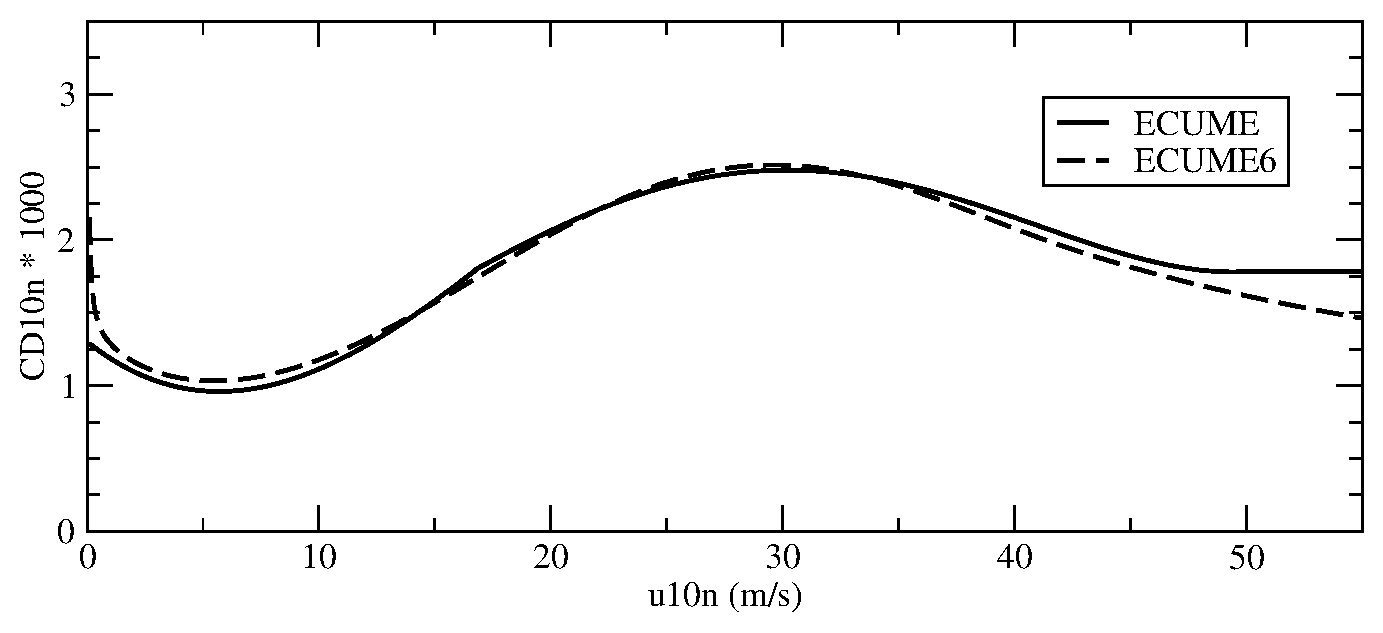
\includegraphics[width=19.4pc,clip=true]{EPS/new_cdn.eps}
 \centering\includegraphics[width=19.4pc,clip=true]{EPS/parun.eps}
 \centering\includegraphics[width=19.4pc,clip=true]{EPS/new_chn.eps}
 \centering\includegraphics[width=19.4pc,clip=true]{EPS/partn.eps}
 \centering\includegraphics[width=19.4pc,clip=true]{EPS/new_cen.eps}
 \centering\includegraphics[width=19.4pc,clip=true]{EPS/parqn.eps}
	\caption{Left: Neutral coefficients at 10 meters $C_{D_{10n}}$, $C_{H_{10n}}$ and $C_{E_{10n}}$ in the ECUME 
	(solid line) and derived from the ECUME6 (dashed line) formulations. 
	Right: Neutral parameters at 10 meters $\mathcal{P}_{u_{10n}}$, $\mathcal{P}_{{\theta}_{10n}}$ and $\mathcal{P}_{q_{10n}}$ 
	in the ECUME6 formulation.\label{ecume_coef}}
\end{figure}

The key difference between the two parameterizations is that the original one (\textit{ECUME}, see Belamari, 2005 %\citet{bel05}
for more details) provides formulations
of the neutral exchange coefficients at 10m (drag coefficient $C_{D_{10n}}$, heat coefficient $C_{H_{10n}}$ and 
evaporation coefficient $C_{E_{10n}}$) as functions of the neutral vertical wind gradient between the sea surface and 
10m-height $\Delta u_{10n}$ 
(Figure \ref{ecume_coef}, left part) while the new one (\textit{ECUME6}) provides formulations of derived parameters for the wind
$\mathcal{P}_{u_{10n}}$, potential temperature $\mathcal{P}_{{\theta}_{10n}}$ and specific humidity $\mathcal{P}_{q_{10n}}$
(Figure \ref{ecume_coef}, right part), defined as:
\begin{equation}
\left\{
\begin{array}{l}
	\mathcal{P}_{u_{10n}}=\left(\frac{C_{D_{10n}}}{\sqrt{C_{D_{10n}}}}\right)\times \Delta u_{10n} \\
	\mathcal{P}_{{\theta}_{10n}}=\left(\frac{C_{H_{10n}}}{\sqrt{C_{D_{10n}}}}\right)\times \Delta u_{10n} \\
	\mathcal{P}_{q_{10n}}=\left(\frac{C_{E_{10n}}}{\sqrt{C_{D_{10n}}}}\right)\times \Delta u_{10n} 
\end{array}
\right.
\end{equation}
The definition of these new parameters was motivated by the wide dispersion of the scatterplots providing the observed 
neutral exchange coefficients as a function of the neutral wind at 10 meters, in contrast to those of these new
parameters.\\

As in the two other iterative parameterizations, the ECUME and ECUME6 algorithms begin with a first \textbf{preliminary step} that insures the \textbf{initialization} 
of all the required variables, namely:
\begin{enumerate}
	\item the vertical gradients of the wind, potential temperature and specific humidity at the air-sea interface 
($\Delta u$, $\Delta \theta$ and $\Delta q$)
	\item the corresponding neutral vertical gradients:
$$
\left\{
\begin{array}{l}
	\Delta u_{10n}=\Delta u\\
	\Delta {\theta}_{10n}=\Delta \theta \times d_0\\
	\Delta q_{10n}=\Delta q
\end{array}
\right.
$$
with:
$$
\left\{
\begin{array}{ll}
	d_0=1.2+6.3~10^{-3}\mathit{MAX}(\Delta u-10~,~0) & \mathrm{in~ECUME}\\
	d_0=1.0 & \mathrm{in~ECUME6}
\end{array}
\right.
$$
\end{enumerate}
In ECUME6, an initial guess is also made for the characteristic length scales as initial values of 
$u_*$, ${\theta}_*$ and $q_*$ are required by the convergence criterion:
$$
\left\{
\begin{array}{l}
	u_*=0.04~\Delta u\\
	{\theta}_*=0.04~\Delta \theta\\
	q_*=0.04~\Delta q
\end{array}
\right.
$$

\vspace*{0.2 cm}

As a \textbf{second step}, the \textbf{iterative loop} then insures the computation of:
\begin{enumerate}
	\item the neutral exchange coefficients/parameters as functions of the neutral vertical wind gradient 
between the sea surface and 10m-height $\Delta u_{10n}$:
%%%%%%%%%%%%%%%%%%%%%%%%%
		\begin{center}
\begin{tabular}{|c|c|c|}
\hline
	 & ECUME & ECUME6 \\
\hline
	 & Neutral coefficient & Neutral parameter \\
	Momentum & $C_{D_{10n}}=f_u(\Delta u_{10n})$        & $\mathcal{P}_{u_{10n}}=g_u(\Delta u_{10n})$ \\
	Heat     & $C_{H_{10n}}=f_{\theta}(\Delta u_{10n})$ & $\mathcal{P}_{{\theta}_{10n}}=g_{\theta}(\Delta u_{10n})$ \\
	Moisture & $C_{E_{10n}}=f_q(\Delta u_{10n})$        & $\mathcal{P}_{q_{10n}}=g_q(\Delta u_{10n})$ \\
\hline
\end{tabular}
		\end{center}
%%%%%%%%%%%%%%%%%%%%%%%%%

	\item the characteristic length scales $u_*$, ${\theta}_*$ and $q_*$ derived from the previous coefficients/parameters:
%%%%%%%%%%%%%%%%%%%%%%%%%
		\begin{center}
\begin{tabular}{|c|c|c|}
\hline
	 & ECUME & ECUME6 \\
\hline
	 & \multicolumn{2}{c|}{Scaling parameters}\\
	Momentum & $u_*=\sqrt{C_{D_{10n}}}.\Delta u_{10n}$  & $u_*=\mathcal{P}_{u_{10n}}$ \\
	Heat     & ${\theta}_*=\left(\frac{C_{H_{10n}}}{\sqrt{C_{D_{10n}}}}\right).\Delta {\theta}_{10n}$  
			& ${\theta}_*=\mathcal{P}_{{\theta}_{10n}}\left(\frac{\Delta {\theta}_{10n}}{\Delta u_{10n}}\right)$ \\
	Moisture     & $q_*=\left(\frac{C_{E_{10n}}}{\sqrt{C_{D_{10n}}}}\right).\Delta q_{10n}$  
			& $q_*=\mathcal{P}_{q_{10n}}\left(\frac{\Delta q_{10n}}{\Delta u_{10n}}\right)$ \\
\hline
\end{tabular}
		\end{center}
%%%%%%%%%%%%%%%%%%%%%%%%%
	\item the stability parameter $\zeta$=$z/L$ constrained to be in the range $[$-200.0;0.25$]$,
using for the Monin-Obukhov length $L$ the same approximate formulation as in COARE3.0
(equation \ref{LMO_approx})
	\item the stability functions $\psi_{m}$ and $\psi_{h}$ as $\psi_{q}$ is supposed to be equal to $\psi_{h}$ (section \ref{iterative_param}.4)
	\item and last, the neutral vertical gradients:
$$
\left\{
\begin{array}{l}
\vspace*{0.2 cm}
	\Delta u_{10n}=\Delta u - \frac{u_*}{\kappa}\left[\ln\left(\frac{z}{10}\right)-{\psi}_m(\zeta)\right]\\
\vspace*{0.2 cm}
	\Delta {\theta}_{10n}=\Delta {\theta} - \frac{{\theta}_*}{\kappa}\left[\ln\left(\frac{z}{10}\right)-{\psi}_h(\zeta)\right]\\
	\Delta q_{10n}=\Delta q - \frac{q_*}{\kappa}\left[\ln\left(\frac{z}{10}\right)-{\psi}_q(\zeta)\right]
\end{array}
\right.
$$
\end{enumerate}

\textbf{At the end of the iterative loop}, the final values of the characteristic length scales are then used to derive:
\begin{itemize}

	\item the exchange coefficients $C_D$, $C_H$ and $C_E$ (from equations \ref{eq_COEF}),

	\item the air-sea turbulent fluxes ${\tau}_{\mathit{sea}}$, $H_{\mathit{sea}}$ and ${\mathit{LE}}_{\mathit{sea}}$ 
	(from equations \ref{eq_bulk} in ECUME and \ref{eq_charlength} in ECUME6),

	\item and last, the roughness lengths:
\begin{itemize}
	\item in ECUME, the dynamical roughness length $z_0$ is computed in a single way using the \textit{subgrid} formulation 
(equation \ref{z0_arpege}) with $\beta$=10$^{-5}$

	\item in ECUME6, the dynamical roughness length $z_0$ may be computed in three different ways depending on the 
choice of a dedicated parameter (\textit{KZ0}):
\begin{itemize}
	\item using the \textit{subgrid} formulation with $\beta$=10$^{-5}$ in equation \ref{z0_arpege} if \textit{KZ0}=0
	\item using the relationship of Smith (1988) with $\beta$=0.11 in equation \ref{z0_smith} if \textit{KZ0}=1
	\item from the characteristic length scale $u_*$, using a formulation derived from equation \ref{allstars} if \textit{KZ0}=2:
\begin{equation}
	z_0=z \left(\exp \left[\kappa\frac{\Delta u}{u_*}+{\psi}_m(\zeta)\right]\right)^{-1}
\label{z0_direct}
\end{equation}
\end{itemize}
\end{itemize}
Note that if the dynamical roughness length $z_0$ is computed using the \textit{subgrid} formulation or the relationship of Smith (1988),
the Charnock parameter $\alpha$ may be either constant  
if \textit{CCHARNOCK=\textquotesingle{}OLD\textquotesingle{}} (then $\alpha$=0.021)
or wind dependent as in COARE3.0 (equation \ref{charnockwithwind}) 
if \textit{CCHARNOCK=\textquotesingle{}NEW\textquotesingle{}}.
\end{itemize}

The ECUME and ECUME6 parameterizations include other specific points:

\begin{enumerate}

	\item No waves effects are taken into account in these parameterizations. 

	\item A stochastic perturbation may be applied to the air-sea turbulent fluxes (logical \textit{OPERTFLUX}) in both
parameterizations.

	\item In ECUME, the number of iterations is prescribed (fixed to 10), while in ECUME6 a convergence criterion is used:
the iterative loop is stopped when the difference between the scale parameters of two successive iterations is 
inferior to a prescribed threshold ($10^{-6}$ ms$^{-1}$ for $u_{*}$, $10^{-6}$ K for $\theta_{*}$ and $10^{-9}$ kg/kg for $q_{*}$).
Note that an important effort was done for the ECUME6 algorithm in order to ensure the convergence in maximum 10 iterations 
whatever the meteo-oceanic conditions (Belamari, 2005). %\citep{bel05}

	\item In ECUME, a correction may be applied to the neutral coefficient for humidity (default is \textit{XICHCE}=0):

		$C_{E_{10n}}=C_{E_{10n}}(1-\mathit{XICHCE})+C_{H_{10n}}(\mathit{XICHCE})~~~~~\mathrm{with}~~~~~0.0\leq\mathit{XICHCE}\leq1.0$


\end{enumerate}


\subsubsection{\ref{iterative_param}.4 $~$ Stability functions used in the iterative parameterizations}

The stability functions $\psi_{m}$ and $\psi_{h}$ used in the four iterative parameterizations 
to correct the wind, potential temperature and specific humidity logarithmic profiles in the boundary layer 
according to the atmospheric stratification are all modified Businger's %\nocite{bus71}
functions as detailed hereafter. ECUME* stands for both ECUME and ECUME6, and ${\psi}_*$ represents either
$\psi_{m}$ or $\psi_{h}$ depending on the considered parameter.

You may note that in unstable conditions the stability functions result from two contributions: a \textit{Kansas} part
to represent the classical unstability, and a \textit{Convective} part to take into account the free convection,
with a weight $f$ depending on the Monin-Obukhov stability parameter $\zeta$.
In the MR98 parameterization, a different formulation is used for the weight $f$ but we do not
mention it here as the resulting formulation of the stability functions including the two contributions is 
rigorously equivalent.

%%%%%%%%%%%%%%%%%%%%%%%%%
\begin{table}[!h]
\centering
\begin{tabular}{|c|lc|c|}
\hline
	& & Wind & Potential temperature \\
\hline
	& & & \\
	Stable         & \textbf{MR98}     & \multicolumn{2}{c|}{$\psi_{*}(\zeta)=-4.7~\zeta$}\\
	($\zeta\geq0$) & \textbf{ECUME*}   & \multicolumn{2}{c|}{$\psi_{*}(\zeta)=-7.0~\zeta$}\\
	               & \textbf{COARE3.0} & \multicolumn{2}{c|}{$\psi_{*}(\zeta)=-\left[1+\zeta+\frac{2}{3}\left(\frac{\zeta-14.28}{\exp(\Gamma)}\right)+8.525\right]~~\mathrm{with}~~\Gamma=\mathit{MIN}(50,~0.35\zeta)$}\\
	& & & \\
\hline
	& & & \\
	Unstable    & & \multicolumn{2}{c|}{$\psi_{*}(\zeta)=(1-f)\psi_{*K}+f\psi_{*C}$}\\
	($\zeta<0$) & & \multicolumn{2}{c|}{with $~~f=\frac{\zeta^{2}}{1+\zeta^{2}}$}\\
	& & & \\
	Kansas      & & $\psi_{mK}=2.\ln\left(\frac{1+x}{2}\right)+\ln\left(\frac{1+x^{2}}{2}\right)$ & $\psi_{hK}=2.\ln(\frac{1+x^2}{2})$\\
	            & & $-2.\arctan(x)+\frac{\pi}{2}$ & \\
	            & & \multicolumn{2}{c|}{with:} \\
	            & \textbf{MR98}     & \multicolumn{2}{c|}{$x=(1-16~\zeta)^{\frac{1}{4}}$}\\
		    & \textbf{ECUME*}   & \multicolumn{2}{c|}{$x=(1-16~\zeta)^{\frac{1}{4}}$}\\
		    & \textbf{COARE3.0} & \multicolumn{2}{c|}{$x=(1-15~\zeta)^{\frac{1}{4}}$}\\
	            & & & \\
	Convective  & & \multicolumn{2}{c|}{$\psi_{*C}=\frac{3}{2}\ \ln\left(\frac{1+y+y^2}{3}\right)-\sqrt{3}.\arctan\left(\frac{1+2y}{\sqrt{3}}\right)+\frac{\pi}{\sqrt{3}}$}\\
	            & & \multicolumn{2}{c|}{with:} \\
	            & \textbf{MR98}     & \multicolumn{2}{c|}{$y=(1-12.87~\zeta)^{\frac{1}{3}}$}\\
		    & \textbf{ECUME*}   & \multicolumn{2}{c|}{$y=(1-12.87~\zeta)^{\frac{1}{3}}$}\\
		    & \textbf{COARE3.0} & $y=(1-10.15~\zeta)^{\frac{1}{3}}$ & $y=(1-34.15~\zeta)^{\frac{1}{3}}$ \\
	   & & & \\
\hline
\end{tabular}
\caption{Stability functions used in the iterative parameterizations.
\label{stability_functions}}
\end{table}
%%%%%%%%%%%%%%%%%%%%%%%%%

\vspace*{0.2 cm}


\subsubsection{\ref{iterative_param}.5 $~$ Additional refinements included in the iterative parameterizations}

Each of the four iterative parameterizations may include some refinements as detailed in Table \ref{refinements}.
\begin{enumerate}

	\item \textbf{Salinity correction:} 
A reduction of 2\% may be applied to the saturated vapor pressure $P_{\mathit{sat}}$ used in the computation 
of the specific humidity at the sea surface $q_s$ in order to take into account the decreasing of $P_{\mathit{sat}}$
due to seawater salinity (Kraus, 1972)\nocite{kraus1972}:  
\begin{equation}
	q_{s}=q_{s}(P_{\mathit{sat}})~~~~~\mathrm{with}~~~~~P_{\mathit{sat}}=0.98\times P_{\mathit{sat}}(T_{s})
\end{equation}

	\item \textbf{Explicit dependency to sea surface salinity:}
In ECUME6, if the sea surface salinity (SSS) field is available in the SURFEX surface scheme, an explicit dependency to the SSS
may be used in the computation of both the saturated vapor pressure $P_{\mathit{sat}}$ from which the specific humidity at 
the sea surface $q_s$ is derived (Sharqawy \textit{et al.}, 2010), %\citet{Sharqawy2010}
and the latent heat of seawater vaporization ${\mathcal{L}}_{v}$:
$$
\left\{
\begin{array}{l}
	q_{s}=q_{s}(P_{\mathit{sat}})~~~~~\mathrm{with}~~~~~P_{\mathit{sat}}=P_{\mathit{sat}}(T_{s},SSS)\\
	{\mathcal{L}}_{v}={\mathcal{L}}_{v}(\mathit{SSS})
\end{array}
\right.
$$

	\item \textbf{Wind subgrid correction:}
The relative wind - and therefore the wind gradient - may be increased by a subgrid correction ($w_g$) introduced in order to 
take into account the gustiness impact:
\begin{equation}
	\Delta u=\sqrt{U^2+{w_g}^2}~~~~~~~~~~\mathrm{with}~~~~~~~~~~w_g={\beta}_{\mathit{gust}}({B_F}.z_{\mathit{BL}})^{\frac{1}{3}}
\end{equation}
$z_{\mathit{BL}}$ is the atmospheric boundary layer depth (in meters), ${\beta}_{\mathit{gust}}$ is a constant coefficient,
and ${B_F}$ is the surface buoyancy flux:
		$${B_F}=-g.u_*.\mathcal{F}$$
If $B_F \leq$0, the wind correction $w_g$ is set to a minimal value $w_{g_{\mathit{min}}}$.

	\item \textbf{Wind stress correction} and \textbf{Heat flux correction} due to rainfall:
As rainfall tends to increase the surface drag and to cool the ocean, two additional contributions 
$\tau_{r}$ (Fairall \textit{et al.}, 1996b) %\citep{fbr96}
and $H_{r}$ (Gosnell \textit{et al.}, 1995) %\citep{gfw95}
may be computed in order to correct the surface wind stress and sensible heat flux, respectively:
\begin{equation}
\left\{
\begin{array}{l}
	{\tau}_r=-\gamma~\mathcal{R} \times U\\
	H_r={\mathcal{R}}~{c_{p_{\mathit{lw}}}} {\alpha}_c (T_s-T_a)\left(1+\frac{1}{B}\right)
\end{array}
\right.
\end{equation}
$\mathcal{R}$ denotes the precipitation rate (in kg.s$^{-1}$.m$^{-2}$).
$c_{p_{\mathit{lw}}}$ is the rain specific heat including a dependency to the rain temperature (supposed to be equal to that of the air).
${\alpha}_c$ is a dimensionless parameter called the wet-bulb factor:
\begin{equation}
	{\alpha}_c=\left[1+ \frac{L_r~d_v}{c_{p_d}~d_h} \left(\frac{dq_{\mathit{sat}}}{dT}\right) \right]^{-1}
\end{equation}
where $L_r$ is the latent heat of rain vaporization (in J.kg$^{-1}$), 
$c_{p_d}$ is the specific heat of dry air (in J.K$^{-1}$.kg$^{-1}$),
$d_v$ and $d_h$ are the diffusivities for water vapor (Pruppacher and Klett, 1978) and heat, respectively.
The slope of the saturated specific humidity at atmospheric level $q_{\mathit{sat}}({\theta}_a)$ as a function of the temperature 
is derived from the Clausius-Clapeyron relation:
		$$\frac{dq_{\mathit{sat}}}{dT}=\lambda \left[ \frac{L_r~q_{\mathit{sat}}({\theta}_a)}{R_v~{T_a}^{2}}\right]$$
$B$ is the Bowen ratio:
	$$B= \mu \left(\frac{c_{p_d}}{L_r}\right) \left(\frac{T_s-T_a}{q_s-q_a}\right)$$

	\item \textbf{Webb correction:}
%\nocite{wbb80}
This small correction may be applied to the latent heat flux in order to take into account the air density variations when the humidity 
varies under the evaporation action:
$$LE_{\mathit{Webb}}=\rho_{a}~{\mathcal{L}}_{v}~\overline{w}~q_a$$
where ${\mathcal{L}}_{v}$ is the latent heat of seawater vaporization at sea surface, and $\overline{w}$ is the mean value of the vertical 
speed perturbations: 
$$ \overline{w} = 1.61~\overline{w'q'}+(1+1.61~q_a)\frac{\overline{w'{\theta}'}}{T_a} = -\left[1.61~u_* q_*+(1+1.61~q_a)\frac{u_* {\theta}_*}{T_a}\right] $$

\end{enumerate}

%%%%%%%%%%%%%%%%%%%%%%%%%
\begin{table}[!h]
\centering
\begin{tabular}{|l|c|c|c|c|}
\hline
	                       	& MR98                                              & COARE3.0 & ECUME & ECUME6 \\
\hline
	Salinity correction    	& Yes                                               & Yes      & Yes   & Yes    \\
\hline
	Explicit dependency  	& No                                                & No       & No    & Yes [1] \\
	to sea surface salinity & & & & \\
\hline
				& Yes with:                                         & Yes [2] with: & Yes [2] with: & No \\
				& $w_{g_{\mathit{min}}}$=0.0 ms$^{-1}$              & $w_{g_{\mathit{min}}}$=0.2 ms$^{-1}$ & $w_{g_{\mathit{min}}}$=0.0 ms$^{-1}$ & \\
	Wind subgrid		& ${\beta}_{\mathit{gust}}$=0.6                     & ${\beta}_{\mathit{gust}}$=1.2 & ${\beta}_{\mathit{gust}}$=1.2 & \\
	correction              & $z_{\mathit{BL}}$=650 m                           & $z_{\mathit{BL}}$=600 m & $z_{\mathit{BL}}$=600 m & \\
		       		& $\mathcal{F}=\frac{{{\theta}_v}_{*}}{{\theta}_v}$ 
				& $\mathcal{F}=\frac{{\theta}_{*}+0.61(T_a q_*)}{T_a}$ 
				& $\mathcal{F}=\frac{{{\theta}_v}_{*}-0.61({\theta}_a-T_a)q_*}{T_a}$ & \\
	 			& & & & \\
\hline
	Wind stress correction  & No & Yes [3] with  & Yes [3] with & Yes [3] with  \\
	due to rainfall         &    & $\gamma$=0.85 & $\gamma$=1.0 & $\gamma$=0.85 \\
\hline
	    			& No & Yes with:   & Yes with:                 & Yes with:                 \\
	Heat flux correction    &    & $\lambda$=1 & $\lambda=\frac{R_v}{R_d}$ & $\lambda$=1 \\
	due to rainfall		&    & $\mu$=1     & $\mu=\frac{d_h}{d_v}$     & $\mu=\frac{d_h}{d_v}$ \\
	 			& & & & \\
\hline
\multicolumn{5}{|l|}{[1] If the sea surface salinity field is available in the SURFEX surface scheme.} \\
\multicolumn{5}{|l|}{$~~~~~$ Else, only the standard ``Salinity correction'' is applied.} \\
\hline
\multicolumn{5}{|l|}{[2] Logical \textit{LPWG} in the \textit{NAM\_SEAFLUXn} namelist.} \\
\hline
\multicolumn{5}{|l|}{[3] Logical \textit{LPRECIP} in the \textit{NAM\_SEAFLUXn} namelist.} \\
\hline
\end{tabular}
	\caption{Additional refinements available (or not) in the iterative parameterizations.
\label{refinements}}
\end{table}
%%%%%%%%%%%%%%%%%%%%%%%%%

Note that:
\begin{enumerate}
	\item In the various formulations of the surface buoyancy flux $B_F$, ${\theta}_v$ is the air virtual potential temperature
(equation \ref{eq_thetav}), ${{\theta}_v}_{*}$ is the associated characteristic length scale given by equation \ref{eq_thetavstar}, 
${\theta}_a$ and $T_a$ are the air potential temperature and air temperature, respectively. 
This leads to different formulations in COARE3.0 and ECUME when compared to the (exact) one used in MR98.
	\item In the heat flux correction due to rainfall, $\lambda$ and $\mu$ should be equal to 1 to be fully consistent with 
Gosnell \textit{et al.} (1995). %\citet{gosnell1995}
\end{enumerate}

%%%%%%%%%%%%%%%%%%%%%%%%%%%%%%%%%%%%%%%%%%%%%%%%%%%%%%%%%%%%%%%%%%%%%%%%%%%%%%%%%%%%%%%%%%%%%%%%%%%%%%%%%%%%%%%%%%%%%%%%

\newpage
\section{Coupling with a 1D TKE oceanic model}
\subsection{Coupling objectifs and principles}
The main objective of the coupling is to improve the fine scale air-sea exchanges modelling in the SURFEX surface scheme. To better represent the fine scale air-sea interactions, it is necessary to take into account the oceanic dynamics and the thermal content evolution (Lebeaupin \etal (2007, 2009)) %\citep{leb08a,leb08b}
. \\
\begin{figure}[!b]
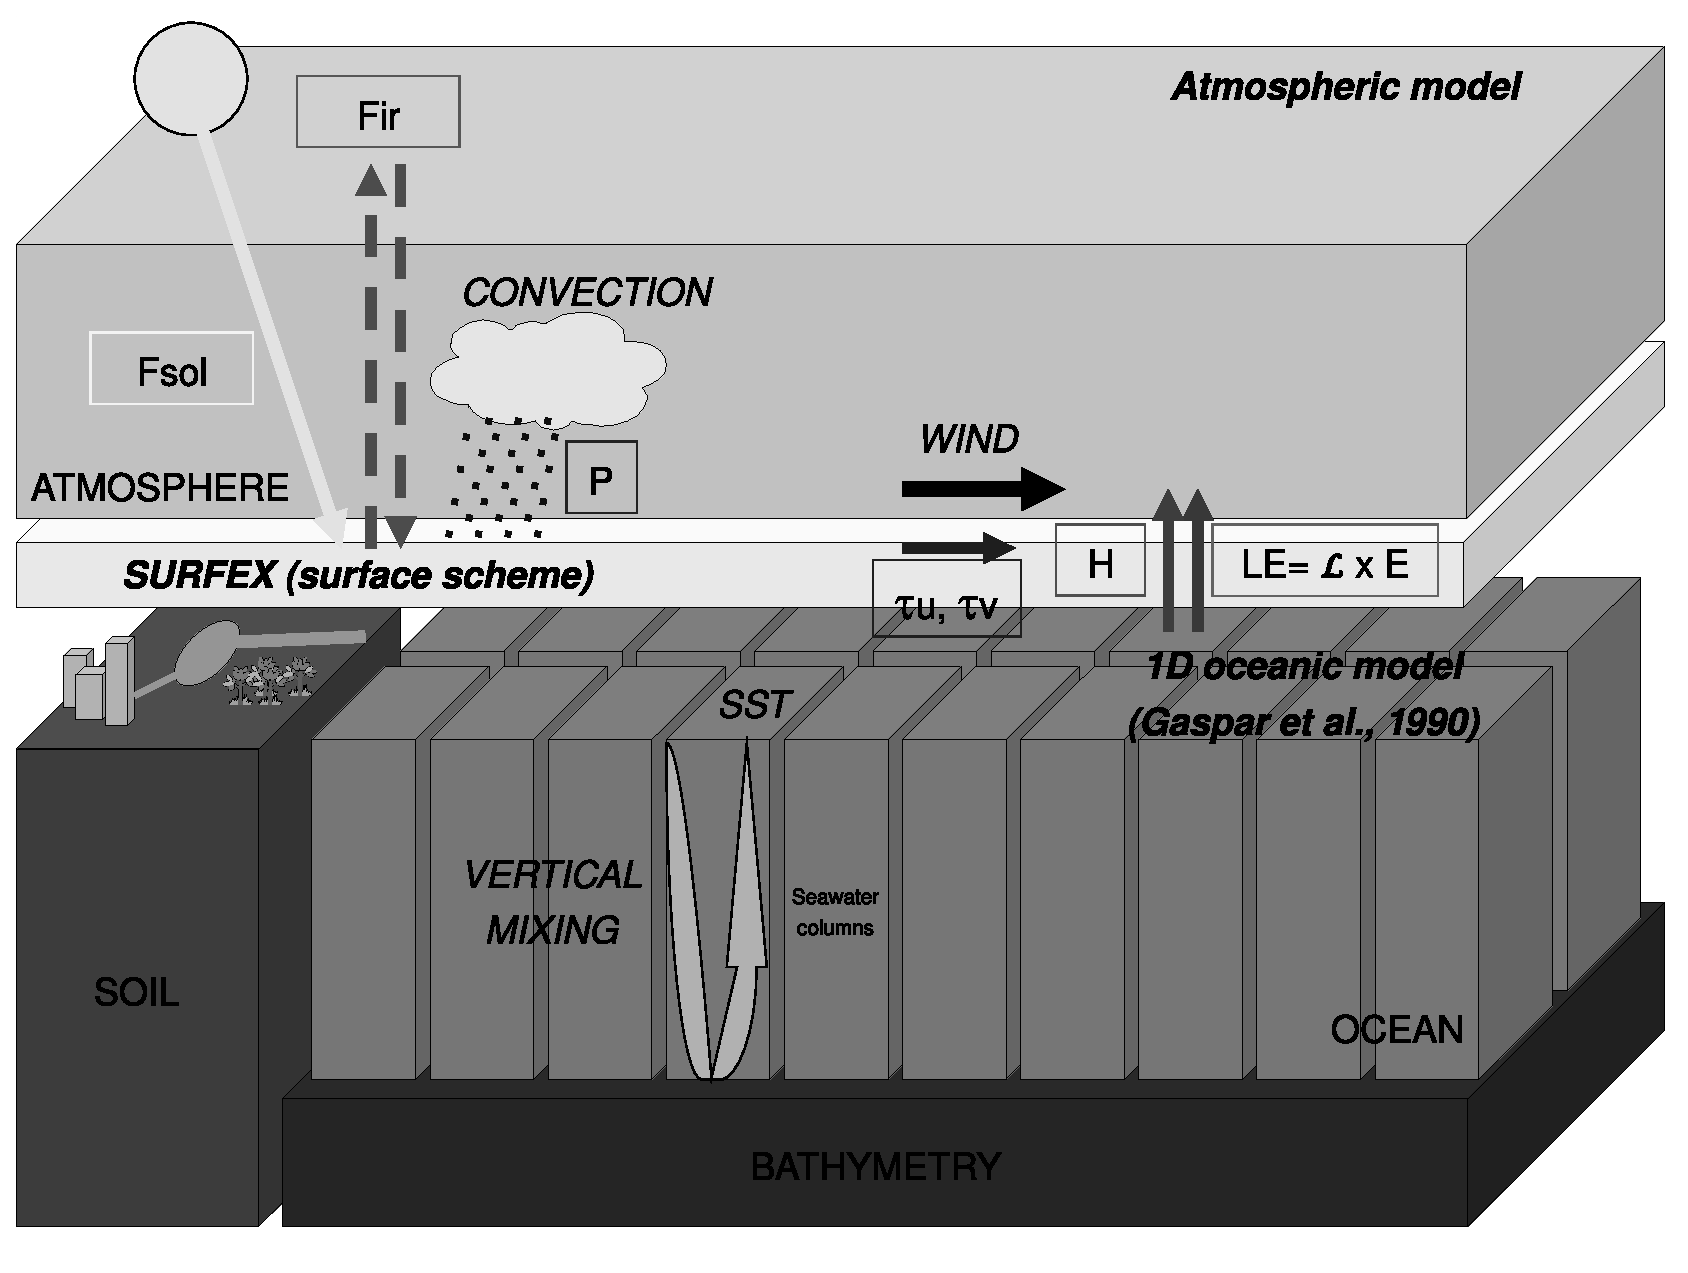
\includegraphics[width=37pc]{EPS/coupling_scheme+processes.NB.eps}
\vspace{-0.75cm}
\caption{The high-resolution ocean-atmosphere coupled system between (MESO-NH) SURFEX and the 1D oceanic model. \label{scheme_coupled_syst}}
\end{figure}
 
The coupled system's principle consists in modelling a seawater column under each grid point containing a fraction of sea and limited by the bottom (Figure \ref{scheme_coupled_syst}). The ocean model used is the uni-dimensional model described by Gaspar \etal (1990) \nocite{Gaspar1990}
 [see section \ref{sct_mod1d}] which allows to represent the oceanic vertical mixing according to a parameterization of turbulence from Bougeault and Lacarr\`ere (1989)\nocite{BL89}
 adapted to ocean. By the turbulent vertical mixing modelling, the 1D ocean model allows to represent the heat, water and momentum exchanges from the superficial oceanic layers in direct interaction with the atmosphere and subjected to radiative effects, to the deepest layers. The turbulent vertical mixing is based on a parameterization of the second-order turbulent moments expressed as a function of the turbulent kinetic energy (Gaspar \etal, 1990). In this formulation, the vertical mixing coefficients are based on the calculation of two turbulent length scales representing upward and downward conversions of turbulent kinetic energy (TKE) into potential energy (Gaspar \etal, 1990). By allowing a response to high frequencies in the surface forcing, the scheme improved the representation of the vertical mixed layer structure, sea surface temperature and upper-layer current (Blanke and Delecluse, 1993 \nocite{Blanke1993}). However, this parameterization fails to properly simulate the mixing in strongly stable layers in the upper thermocline (Large\etal, 1994 \nocite{Large1994}; Kantha and Clayson, 1994 \nocite{Kantha1994}). Consequently, a parameterization of the diapycnal mixing (Large \etal, 1994) was introduced into Gaspar's turbulence parameterization model in order to take into account the effects of the vertical mixing occurring in the thermocline (Josse, 1999 \nocite{Josse1999}). This non local source of mixing, mainly due to internal wave breaking and current shear between the mixed layer and upper thermocline, impacts the temperature, salinity, momentum and turbulent kinetic energy inside the mixed layer particularly during restratification periods. This parameterization was widely used, for instance to study successfully the diurnal cycle in the Equatorial Atlantic (Wade \etal, 2011 \nocite{Wade2011}), the Equatorial Atlantic cold tongue (Giordani \etal, 2011 \nocite{Giordani2011}), the production of modal waters in the North-East Atlantic (Giordani \etal, 2005b \nocite{Giordani2005b}) or to derive surface heat flux corrections (Caniaux \etal, 2005b \nocite{Caniaux2005b}). Note that horizontal and vertical advections can be easily prescribed in the 1D-mixing model to perform realistic simulations in heterogeneous situations.

\subsection{Description of the 1D oceanic model in TKE equation \label{sct_mod1d}}
The 1D model includes a prognostic equation for the turbulent kinetic energy (e) with a 1.5 order closure. The other prognostic variables are the temperature (T), the salinity (S), and the current [$\vec{u}=(u,v)$]. 

\subsubsection{Prognostic equations for T, S, u and v}
Each of the prognostic variables ($\alpha$) is decomposed in a mean value ($\overline{\alpha}$) and a perturbation around this mean value ($\alpha '$), so $\alpha=\overline{\alpha}+\alpha '$. 
For each seawater column, T, S, u and v evolve under the turbulent vertical mixing effect. This mixing depends of air-sea interface fluxes. 

The conservative equations are:
\begin{equation}
\left\{
\begin{array}{l}
\frac{\partial T}{\partial t}=\frac{F_{sol}}{\rho_{0}c_{p}}\frac{\partial I(z)}{\partial z}-\frac{\partial \overline{T'w'}}{\partial z}\\
\\
\frac{\partial S}{\partial t}=-\frac{\partial \overline{S'w'}}{\partial z}\\
\\
\frac{\partial \vec{u} 
}{\partial t}=-f\vec{k}\times \vec{u}-\frac{\partial \overline{\vec{u}'w'}}{\partial z}
\end{array}
\right.
\end{equation}

\noindent where $w$ is the vertical velocity, $\rho_{0}$ is a reference density, $c_{p}$ is the specific heat, $f$ is the Coriolis parameter. $\vec{k}$ is the unit vertical along the vertical, $F_{sol}$ is the solar radiation received by the surface, and $I(z)$ is the solar radiation fraction reaching the depth z ($I(z)$ function decreases exponentially with depth). 

The conditions at the top of the model (z=0) are:
\begin{equation}
\left\{
\begin{array}{l}
-\overline{T'w'}(0)=\frac{F_{nsol}}{\rho_{0}c_{p}}=\frac{H+LE+F_{ir}}{\rho_{0}c_{p}}\\
\\
-\overline{S'w'}(0)=\frac{E-P}{\rho_{0}c_{p}}\\
\\
-\overline{\vec{u}'w'}(0)=\frac{\vec{\tau}}{\rho_{0}c_{p}}\\
\end{array}
\right.
\label{eq_mod1D_interface}\end{equation}

\textbf{Fluxes are positive here downwards. }\\

Finally, the forcing variables to give to the oceanic model are:
\begin{itemize}
\item the solar radiation $F_{sol}$
\item the infra-red radiation $F_{ir}$
\item the evaporation rate $E$ proportional to the latent heat flux $E=\frac{LE}{\mathcal{L}}$
\item the sensible heat flux $H$
\item the zonal and meridional stress components $\vec{\tau}=(\tau_{u},\tau_{v})$
\item the precipitation rate $P$
\end{itemize}
$F_{nsol}$ is defined as the sum of the sensible H, the latent heat flux LE and the infra-red radiation $F_{ir}$ and is named non-solar flux. 


The closure relationships are given by: 
\begin{equation}
\left\{
\begin{array}{l}
-\overline{T'w'}=K_{h}\frac{\partial \overline{T}}{\partial z}\\
\\
-\overline{S'w'}=K_{s}\frac{\partial \overline{S}}{\partial z}\\
\\
-\overline{\vec{u}'w'}=K_{m}\frac{\partial \overline{\vec{u}}}{\partial z}
\end{array}
\right.
\end{equation}

The $K_{*}$ are diffusivity coefficients linked to the turbulent kinetic energy by: 
\begin{equation}
K=c_{k}l_{k}\overline{e}^{\frac{1}{2}}=K_{h}=K_{s}=\frac{K_{m}}{Prt}\simeq K_{m}
\end{equation}

\noindent where $c_{k}$ is a constant to determine; $l_{k}$ is a mixing length and $Prt$ is the Prandlt's number. 

\subsubsection{Prognostic equation for turbulent kinetic energy}
The equation for TKE $e=\frac{1}{2}(u'^{2}+v'^{2}+w'^{2})$ is given by:
\begin{equation}
\frac{\partial \overline{e}}{\partial t}=-\frac{\partial}{\partial z}\left(\overline{e'w'}+\frac{\overline{p'w'}}{\rho_{0}}\right)-\overline{\vec{u'}w'}\times \frac{\partial \overline{\vec{u}}}{\partial z}+\overline{b'w'}-\epsilon
\end{equation}
\noindent where $p$ is pressure; $\epsilon=c_{\epsilon}l_{\epsilon}\overline{e}^{\frac{3}{2}}$ is dissipation; $b=g\frac{\rho-\rho_{0}}{\rho_{0}}$ is the buoyancy. The seawater density is diagnosed from temperature and salinity:
$$\rho=\rho_{0}+(T-T_{ref})\times[-0.19494-0.49038(T-T_{ref})]+0.77475(S-S_{ref})$$
where $T_{ref}=13.5$ °C, $S_{ref}=32.6$ psu and $\rho_{0}=1024.458$ kg/m$^{3}$. 

The vertical TKE flux is parameterized:
\begin{equation}
-\left(\overline{e'w'}+\frac{\overline{p'w'}}{\rho_{0}}\right)=K_{e}\frac{\partial \overline{e}}{\partial z}
\end{equation}
with
\begin{equation}
K_e=c_{\epsilon}l_{\epsilon}\overline{e}^{\frac{1}{2}}
\end{equation}

The Bougeault and Lacarr\`ere %\citet{bou89}
 mixing length are:
\begin{equation}
l_{\epsilon}=(l_{u}l_{d})^{\frac{1}{2}}
\end{equation}
\begin{equation}
l_{k}=min(l_{u},l_{d})~ pour~k=h,s~and~m
\end{equation}

$l_{u}$ and $l_{d}$ (for ``up'' and ``down'') are estimated as the upwards and downwards distances for which the kinetic energy is transformed in potential energy:
\begin{equation}
\overline{e}(z)=\frac{g}{\rho_{0}}\int_{z}^{z+l_{u}}\lbrack\overline{\rho}(z)-\rho(z')\rbrack dz'
\end{equation} 
\begin{equation}
\overline{e}(z)=\frac{g}{\rho_{0}}\int_{z}^{z-l_{d}}\lbrack\overline{\rho}(z)-\rho(z')\rbrack dz'
\end{equation} 

\subsubsection{Discretization}
The temporal integration scheme is a semi-implicit scheme for T and S. For the horizontal current $\vec{u}=(u,v)$, the integration scheme is implicit/semi-implicit. 

The discretization is here described in detail for the temperature. The same could be done for the salinity, the TKE and the current in complex notation ($\vec{u}\rightarrow u+iv$, $i^{2}=-1$). 

The equation
$$
\frac{\partial T}{\partial t}=\frac{F_{sol}}{\rho_{0}c_{p}}\frac{\partial I(z)}{\partial z}-\frac{\partial}{\partial z}\left(-K\frac{\partial \overline{T}}{\partial z}\right)$$
is decomposed as:
\begin{equation}
\frac{T^{t+1}_{k}-T^{t}_{k}}{\Delta t}=\frac{F_{sol}}{\rho_{0}c_{p}}\frac{\partial I(z)}{\partial z}+\frac{1}{\Delta z_{2}(k)}\lbrack K(k+1)\frac{T^{t+1}_{k+1}-T^{t+1}_{k}}{\Delta z_{1}(k)}-K(k)\frac{T^{t+1}_{k}-T^{t+1}_{k-1}}{\Delta z_{1}(k)}\rbrack
\end{equation}
$$T^{t+1}_{k-1}\left(-\frac{K(k)}{\Delta z_{1}\Delta z_{2}}\right)+T^{t+1}_{k}\left(\frac{1}{\Delta t}+\frac{K(k+1)-K(k)}{\Delta z_{1}\Delta z_{2}}\right)+T^{t+1}_{k+1}\left(-\frac{K(k+1)}{\Delta z_{1}\Delta z_{2}}\right)=\frac{1}{\Delta t}T^{t}_{k}+\frac{F_{sol}}{\rho_{0}c_{p}}\frac{\partial I}{\partial z}$$

In a matricial writing following the vertical levels (k):
\begin{equation}
\lbrack\mathcal{M}\rbrack\left(T^{t+1}\right)=\frac{1}{\Delta t}\left(T^{t}\right)+\lbrack\frac{F_{sol}}{\rho_{0}c_{p}}\frac{\partial I(z)}{\partial z}\rbrack
\end{equation}
\begin{equation}
\lbrack\mathcal{M}\rbrack=\left(
\begin{array}{ccccccc}
. & . & 0 & & & & \\
. & . & . & 0 & & & \\
0 & \beta_{k} & \alpha_{k} & \gamma_{k} & 0 & &\\
- & - & - & - & - & - & - \\
 & & & 0 & . & . & .\\
 & & & & 0 & . & .\\
\end{array}
\right)
\end{equation}
$$\alpha_{k}=\frac{1}{\Delta t}+\frac{K(k+1)-K(k)}{\Delta z_{1}\Delta z_{2}}$$
$$\beta_{k}=-\frac{K(k)}{\Delta z_{1}\Delta z_{2}}$$
$$\gamma_{k}=-\frac{K(k+1)}{\Delta z_{1}\Delta z_{2}}$$

$\lbrack\mathcal{M}\rbrack$ is a tri-diagonal matrix to invers. \\

The vertical grid must be a z-coordinates grid as described by Fig. \ref{grille1}. 
\begin{figure}[!h]
\centering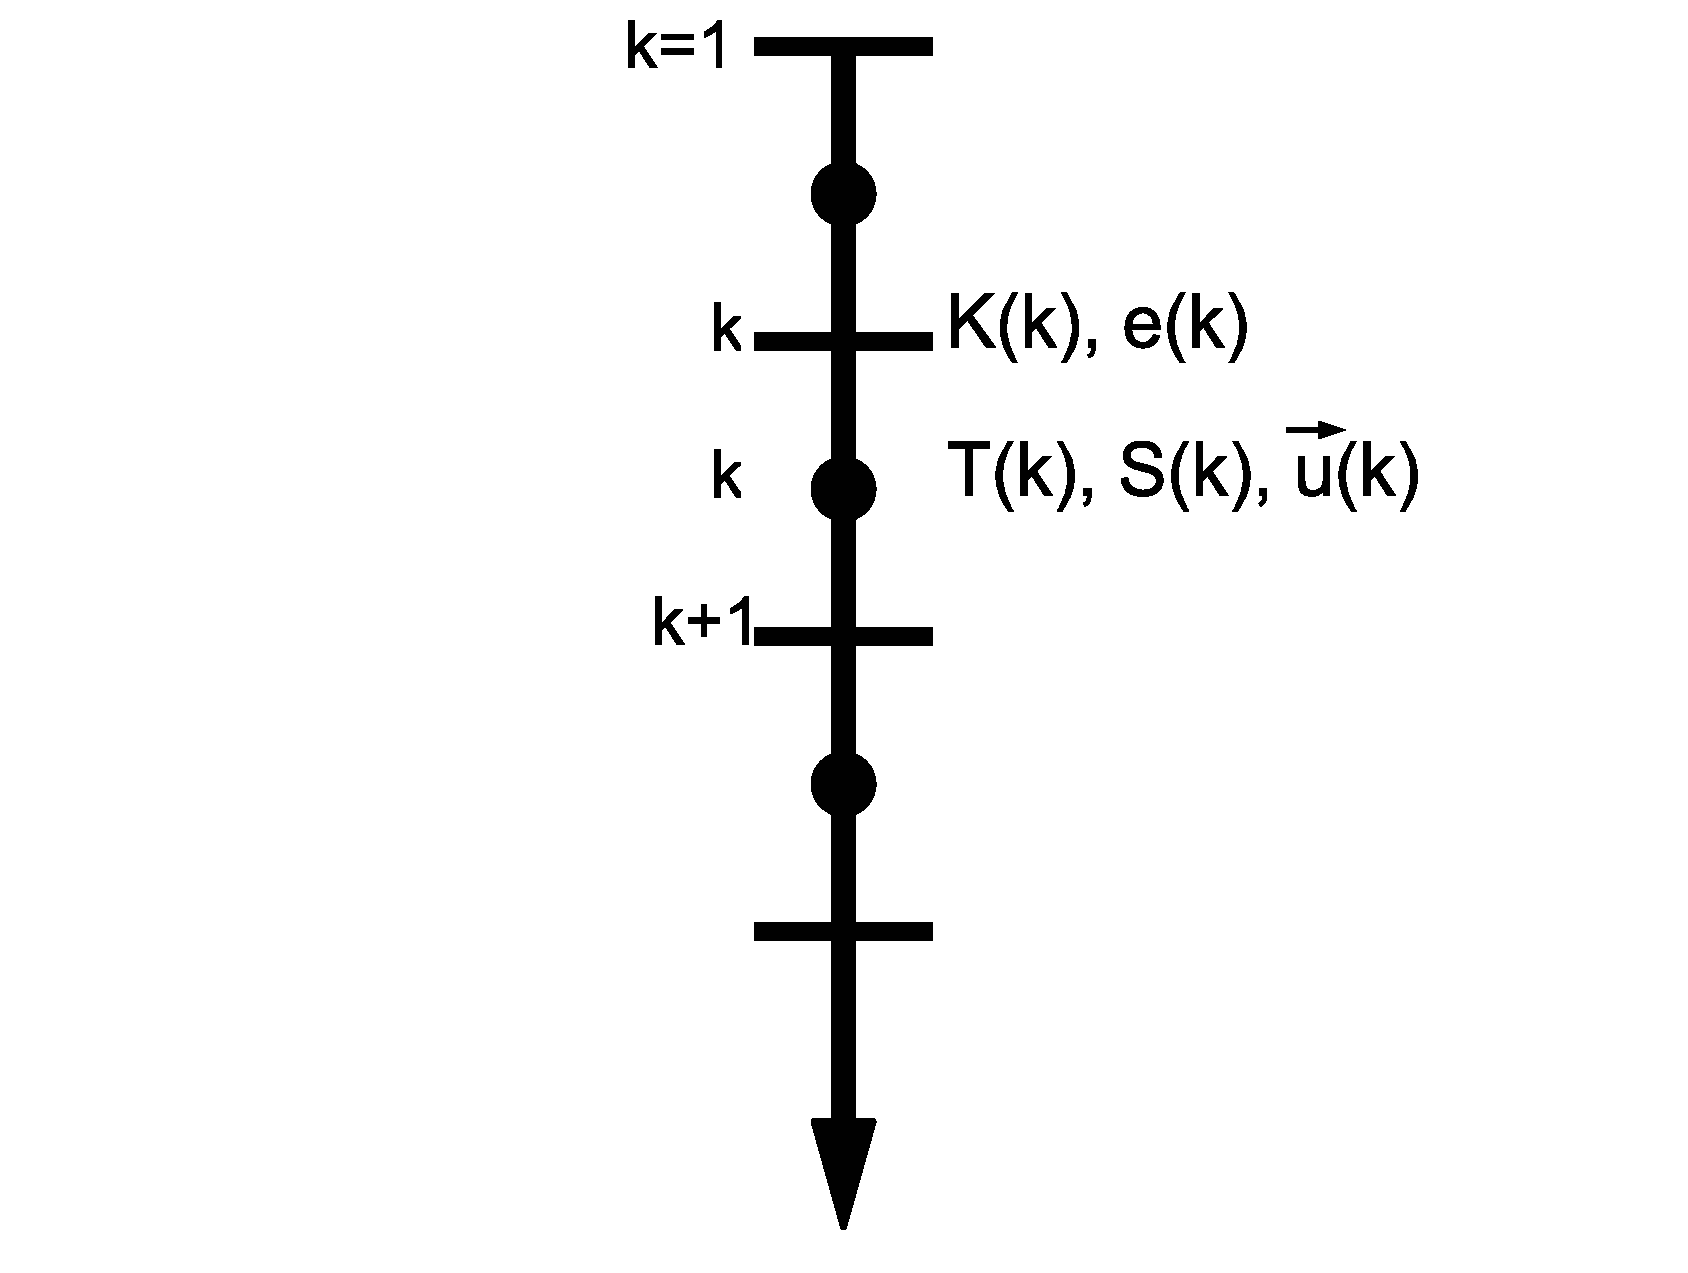
\includegraphics[height=14.5pc]{EPS/grille1D.eps}
\caption{Vertical grid description of the 1D oceanic model from Gaspar et al. (1990) %\citet{gas90b}
.  \label{grille1}}
\end{figure}

To take into account the bathymetry effects on the oceanic vertical mixing, we introduced a bathymetry index (as the sea-land mask) which is worth 0 for free sea and 1 for levels under the sea-bed. For the vertical levels which have a bathymetry index equal to 1, we impose the prognostic variables values equal to the last free-sea level values. The 1D model thus does not carry out any energy transfer towards or coming from the bottom. Only the energy contained in the higher free levels is taken into account. 

We also introduced a diagnosis of mixed layer depth. The mixed layer base is diagnosed with an arbitrary criterion on the density profile: we assume that the thermocline corresponds to the vertical level for which the seawater density is superior to a 0.02 kg m$^{-3}$ variations compared to the density for a reference level (taken at 5m depth).  

Finally, the oceanic model must be initialized in temperature, salinity and current either from an oceanic analysis or from climatologies. 
%%%%%%%%%%%%%%%%%%%%%%%%%%%%%%%%%%%%%%%%%%%%%%%%%%%%%%%%%%%%%%%%%%%%%%%%%%%%%%
\clearpage


%\section{Inland water: Flake model}

%plm
%%%%%%%%%%%%%%%%%%%%%%%%%%%%%%%%%%%%%%%%%%%%%%%%%%%%%%%%%%%%%%%%%%%%%%%%%
%% 
%% Parameterization of Lakes in Numerical Weather Prediction.
%% Description of a Lake Model.
%% by DM
%% COSMO Technical Report No. 11 
%% 
%%%%%%%%%%%%%%%%%%%%%%%%%%%%%%%%%%%%%%%%%%%%%%%%%%%%%%%%%%%%%%%%%%%%%%%%%

%%%%%%%%%%%%%%%%%%%%%%%%%%%%%%%%%%%%%%%%%%%%%%%%%%%%%%%%%%%%%%%%%%%%%%%%%
%% Newcommands for refs
% \input{$HOME/LaTeX/jrn4rfs.incl_tex}
\newcommand{\ag}[3]{{\it Adv.\ Geophys.}, {\bf #1}, #2--#3.}\vspace{-1.4mm}
\newcommand{\arfm}[3]{{\it Ann.\ Rev.\ Fluid Mech.},\ {\bf #1},\ #2--#3.}
\newcommand{\asj}[3]{{\it Astrophys.\ J.},\ {\bf #1},\ #2--#3.}\vspace{-1.4mm}
\newcommand{\ao}[3]{{\it Atmosphere-Ocean},\ {\bf #1},\ #2--#3.}\vspace{-1.4mm}
\newcommand{\bamso}[3]{{\it Bull.\ Amer.\ Met.\ Soc.},\ {\bf #1},\ #2--#3.}\vspace{-1.4mm}
\newcommand{\blm}[3]{{\it Boundary-Layer Meteorol.},\ {\bf #1},\ #2--#3.}\vspace{-1.4mm}
\newcommand{\bpa}[3]{{\it Beitr.\ Phys.\ Atmosph.},\ {\bf #1},\ #2--#3.}\vspace{-1.4mm}
\newcommand{\cldyn}[3]{{\it Clim.\ Dynam.},\ {\bf #1},\ #2--#3.}\vspace{-1.4mm}
\newcommand{\crst}[3]{{\it Cold.\ Reg.\ Sci.\ Technol.},\ {\bf #1},\ #2--#3.}\vspace{-1.4mm}
\newcommand{\dan}[3]{{\it Dokl.\ Akad.\ Nauk SSSR.},\ {\bf #1},\ #2--#3.}\vspace{-1.4mm}
\newcommand{\dao}[3]{{\it Dyn.\ Atmos.\ Oceans},\ {\bf #1},\ #2--#3.}\vspace{-1.4mm}
\newcommand{\dsr}[3]{{\it Deep-Sea Res.},\ {\bf #1},\ #2--#3.}\vspace{-1.4mm}
\newcommand{\ems}[3]{{\it Environ.\ Modell.\ Softw.},\ {\bf #1},\ #2--#3.}\vspace{-1.4mm}
\newcommand{\fao}[3]{{\it Izv.\ Akad.\ Nauk SSSR. Fizika Atmosfery i Okeana},\ {\bf #1},\ #2--#3.}\vspace{-1.4mm}
\newcommand{\gfd}[3]{{\it Geophys.\ Fluid Dyn.},\ {\bf #1},\ #2--#3.}\vspace{-1.4mm}
\newcommand{\jam}[3]{{\it J.\ Appl.\ Meteorol.},\ {\bf #1},\ #2--#3.}\vspace{-1.4mm}
\newcommand{\jas}[3]{{\it J.\ Atmos.\ Sci.},\ {\bf #1},\ #2--#3.}\vspace{-1.4mm}
\newcommand{\jcli}[3]{{\it J.\ Climate},\ {\bf #1},\ #2--#3.}\vspace{-1.4mm}
\newcommand{\jcp}[3]{{\it J.\ Comput.\ Phys.},\ {\bf #1},\ #2--#3.}\vspace{-1.4mm}
\newcommand{\jcg}[3]{{\it J.\ Crystal Growth},\ {\bf #1},\ #2--#3.}\vspace{-1.4mm}
\newcommand{\jfe}[3]{{\it J.\ Fluid Eng.},\ {\bf #1},\ #2--#3.}\vspace{-1.4mm}
\newcommand{\jfm}[3]{{\it J.\ Fluid Mech.},\ {\bf #1},\ #2--#3.}\vspace{-1.4mm}
\newcommand{\jgr}[3]{{\it J.\ Geophys.\ Res.},\ {\bf #1},\ #2--#3.}\vspace{-1.4mm}
\newcommand{\jgrnew}[4]{{\it J.\ Geophys.\ Res.}, {\bf #1}(#2), #3, #4.}\vspace{-1.4mm}
\newcommand{\jhy}[3]{{\it J.\ Hydrometeorology}, {\bf #1}, #2--#3.}\vspace{-1.4mm}
\newcommand{\jmr}[3]{{\it J.\ Marine Res.},\ {\bf #1},\ #2--#3.}\vspace{-1.4mm}
\newcommand{\jplr}[3]{{\it J.\ Plankton Res.},\ {\bf #1},\ #2--#3.}\vspace{-1.4mm}
\newcommand{\jpo}[3]{{\it J.\ Phys.\ Oceanogr.},\ {\bf #1},\ #2--#3.}\vspace{-1.4mm}
\newcommand{\jweia}[3]{{\it J.\ Wind End.\ Industr.\ Aerodyn.},\ {\bf #1},\ #2--#3.}\vspace{-1.4mm}
\newcommand{\lio}[3]{{\it Limnol.\ Oceanogr.},\ {\bf #1},\ #2--#3.}\vspace{-1.4mm}
\newcommand{\loc}[3]{{\it Limnology and Oceanography}, {\bf #1},\ #2--#3.}\vspace{-1.4mm}
\newcommand{\mwr}[3]{{\it Mon.\ Weather Rev.},\ {\bf #1},\ #2--#3.}\vspace{-1.4mm}
\newcommand{\nat}[3]{{\it Nature},\ {\bf #1},\ #2--#3.}\vspace{-1.4mm}
\newcommand{\noh}[3]{{\it Nordic Hydrology},\ {\bf #1},\ #2--#3.}\vspace{-1.4mm}
\newcommand{\phf}[3]{{\it Phys.\ Fluids},\ {\bf #1},\ #2--#3.}\vspace{-1.4mm}
\newcommand{\po}[3]{{\it Prog.\ Oceanogr.},\ {\bf #1},\ #2--#3.}\vspace{-1.4mm}
\newcommand{\qj}[3]{{\it Quart.\ J.\ Roy.\ Meteorol.\ Soc.},\ {\bf #1},\ #2--#3.}\vspace{-1.4mm}
\newcommand{\rg}[3]{{\it Rev.\ Geophys.},\ {\bf #1},\ #2--#3.}\vspace{-1.4mm}
\newcommand{\rgsp}[3]{{\it Rev.\ Geophys.\ Space Phys.},\ {\bf #1},\ #2--#3.}\vspace{-1.4mm}
\newcommand{\sci}[3]{{\it Science},\ {\bf #1},\ #2--#3.}\vspace{-1.4mm}
\newcommand{\tel}[3]{{\it Tellus},\ {\bf #1},\ #2--#3.}\vspace{-1.4mm}
\newcommand{\vivl}[3]{{\it Verh.\ Internat.\ Ver.\ Limnol.},\ {\bf #1},\ #2--#3.}\vspace{-1.4mm}
\newcommand{\wrr}[3]{{\it Water Resour.\ Res.},\ {\bf #1},\ #2--#3.}\vspace{-1.4mm}
\newcommand{\wea}[3]{{\it Weather},\ {\bf #1},\ #2--#3.}\vspace{-1.4mm}
%% Useful newcommands
%\newcommand{\etal}{{et al.\ }}
% \newcommand{\eg}{{e.g.\ }}
% \newcommand{\ie}{{i.e.\ }}
% \newcommand{\para}{ }
% \newcommand{\pa}{\\}
% \newcommand{\tabline}{\hline}
%\newcommand{\beq}[1]{\begin{eqnarray}\label{{#1}}}
%\newcommand{\beq}{\begin{eqnarray}}
%\newcommand{\eeq}{\end{eqnarray}}
\newcommand{\beqn}{\begin{eqnarray*}}
\newcommand{\eeqn}{\end{eqnarray*}}
%%%%%%%%%%%%%%%%%%%%%%%%%%%%%%%%%%%%%%%%%%%%%%%%%%%%%%%%%%%%%%%%%%%%%%%%%

%\newpage

\section{Inland Water: Lake Model FLake}

\nopagebreak 
%
\noindent
In this section, a lake model (parameterisation scheme) capable of predicting the temperature structure
of lakes of various depth on time scales from a few hours to many years is presented.
A detailed description of the model, termed FLake, is given in Mironov (2010).
FLake is an integral (bulk) model.
It is based on a two-layer parametric representation of the evolving temperature profile within the water column
and on the integral energy budget for these layers.
The structure of the stratified layer between the upper mixed layer and the basin bottom, the lake thermocline,
is described using the concept of self-similarity (assumed shape) of the temperature-depth curve.
The same concept is used to describe the temperature structure
of the thermally-active upper layer of bottom sediments and of the ice and snow cover.
An entrainment equation for the depth of a convectively-mixed layer
and a relaxation-type equation for the depth of a wind-mixed layer
in stable and neutral stratification are developed
on the basis of the turbulence kinetic energy (TKE) equation integrated over the mixed layer.
Both mixing regimes are treated with due regard for the volumetric character of solar radiation heating.
Simple thermodynamic arguments are invoked to develop the evolution equations for the ice and snow depths.
The system of ordinary differential equations for the time-dependent prognostic quantities
that characterise the evolving temperature profile, see Figs.~\ref{ftr_T_sch_2media} and \ref{ftr_T_sch_4media}, is closed with algebraic (or transcendental) equations for diagnostic quantities,
such as the heat flux through the lake bottom and the equilibrium mixed-layer depth in stable or neutral stratification.

The resulting lake model is computationally very efficient but still incorporates much of the essential physics.

Within FLake, the lake water is treated as a Boussinesq fluid, i.e. the water density is taken to be constant equal
to the reference density except when it enters the buoyancy term in the TKE equation and the expression for the buoyancy frequency.

The other thermodynamic parameters are considered constant except for the snow density and the snow heat conductivity.

%
\begin{figure} %[h]
\begin{center}
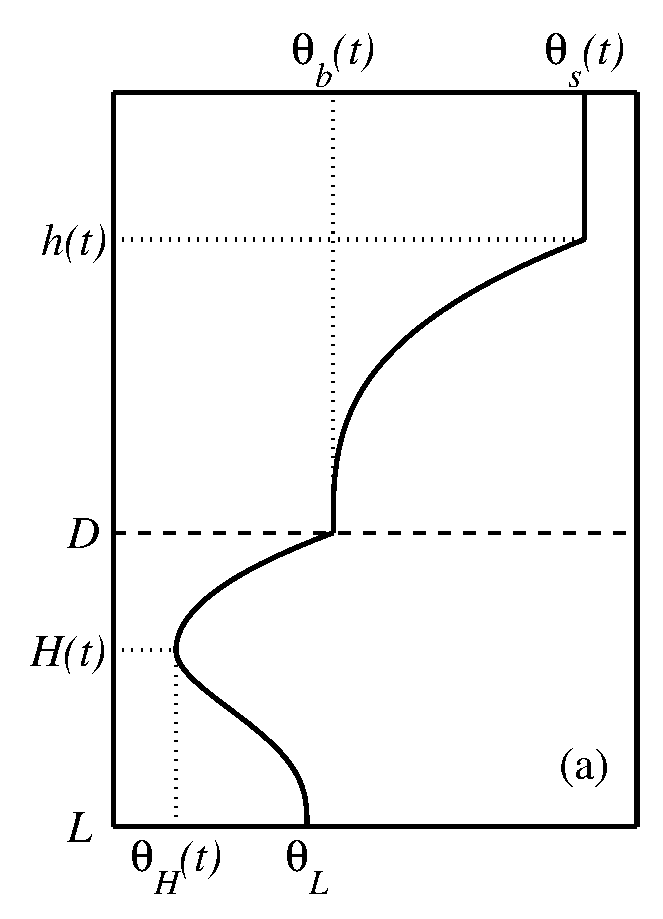
\includegraphics[width=11.5cm]{EPS/f_T_z_MLTBS_A_flk.eps}
\begin{minipage}{0.9\textwidth}
\caption{Schematic representation of the temperature profile
in the mixed layer, in the thermocline, 
and in the thermally active layer of bottom sediments.
The evolving temperature profile is specified by several time-dependent quantities. 
These are 
the mixed-layer temperature $\theta_s(t)$ and its depth $h(t)$,
the temperature $\theta_b(t)$ at the water-bottom sediment interface,
the shape factor $C_{\theta}(t)$ with respect to the temperature profile in the thermocline,
the temperature $\theta_H(t)$ at the lower boundary of the upper layer of bottom sediments
penetrated by the thermal wave, and the depth $H(t)$ of that layer.
The temperature $\theta_{L}$ at the outer edge $z=L$
of the thermally active layer of bottom sediments is constant.}
\label{ftr_T_sch_2media}
\end{minipage}
\end{center}
\end{figure}
%
%
\begin{figure} %[h]
\begin{center}
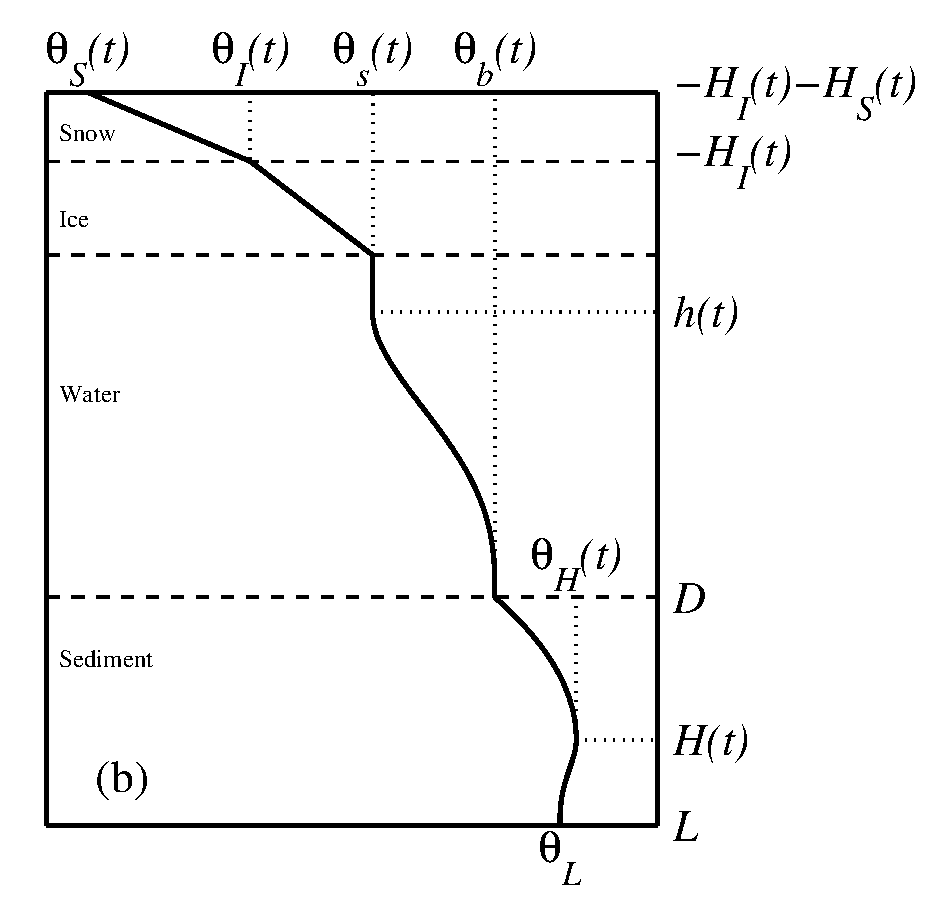
\includegraphics[width=15.0cm]{EPS/f_T_z_ISMLTBS_B_flk.eps}
\begin{minipage}{0.9\textwidth}
\caption{
Apart from $\theta_s(t)$, $h(t)$, $\theta_b(t)$, $C_{\theta}(t)$, $\theta_H(t)$, and $H(t)$   
(see Fig.~\ref{ftr_T_sch_2media}), 
four additional quantities are computed in case the lake is covered by ice and snow. 
These are 
the temperature $\theta_S(t)$ at the air-snow interface,
the temperature $\theta_I(t)$ at the snow-ice interface,
the snow depth $H_S(t)$, and the ice depth $H_I(t)$.}
\label{ftr_T_sch_4media}
\end{minipage}
\end{center}
\end{figure}
%


\subsection{Equation of State}\label{eqstate}
\nopagebreak 
%
\noindent
We utilise the quadratic equation of state of the fresh water, 
%
\beq\label{eqstate2}
\rho_w = \rho_r\left[1-\frac{1}{2}a_T
\left(\theta-\theta_r\right)^2 \right] ,
\eeq
%
where $\rho_w$ is the water density, 
$\rho_r=999.98\approx1.0\cdot10^3$~kg$\cdot$m$^{-3}$ is the maximum density 
of the fresh water at the temperature $\theta_r=277.13$~K, 
and $a_T=1.6509\cdot 10^{-5}$~K$^{-2}$ is an empirical 
coefficient (Farmer and Carmack (1981)\nocite{farmer1981}). 
Equation (\ref{eqstate2}) is the simplest equation of state that 
accounts for the fact that the temperature of maximum density of 
the fresh water exceeds its freezing point 
$\theta_f=273.15$~K. 
According to Eq.~(\ref{eqstate2}), 
the thermal expansion coefficient 
$\alpha_T$ and the buoyancy parameter $\beta$ 
depend on the water temperature, 
%
\beq\label{buopar}
\beta(\theta) = g\alpha_T(\theta) = ga_T(\theta-\theta_r) ,
\eeq
%
where $g=9.81$~m$\cdot$s$^{-2}$ is the acceleration due to gravity.


\subsection{The Water Temperature}\label{wattem}
\nopagebreak 
%
\subsubsection{Parameterization of the Temperature Profile 
and the Heat Budget}\label{heatbudg_WC}
\nopagebreak 
%
\noindent
We adopt the following two-layer parameterization of the vertical temperature profile: 
%
\beq\label{Tprof_ML_T}
\theta = \left\{
\begin{array}{lll}
 \theta_s & \; \; \; \; \mbox{at} & \; \; 0\leq z\leq h \\ 
 \theta_s - (\theta_s-\theta_b)\Phi_{\theta}(\zeta) & 
\; \; \; \; \mbox{at} & \; \; h \leq z \leq D , 
\end{array}
\right.
\eeq
%
where 
$\Phi_{\theta}\equiv\left(\theta_s-\theta\right)/\left(\theta_s-\theta_b\right)$
is a dimensionless function of dimensionless depth 
\linebreak[4]
$\zeta\equiv\left(z-h\right)/\left(D-h\right)$.
The thermocline extends from the mixed-layer outer edge $z=h$ to the basin bottom $z=D$. Hereinafter the arguments of functions dependent on time and depth are not indicated (cf. Figs. \ref{ftr_T_sch_2media} and \ref{ftr_T_sch_4media} ). 

According to Eq.~(\ref{Tprof_ML_T}), 
$h$, $D$, $\theta_s$, $\theta_b$, and the mean temperature of the water column, 
\mbox{$\overline{\theta}\equiv D^{-1}\int_0^D\theta dz$}, 
are related through 
%
\beq\label{TemDepth_Rel} 
\overline{\theta} = \theta_s - C_{\theta}(1-h/D)(\theta_s-\theta_b) , 
\eeq
%
where 
%
\beq\label{ShapeFac_T} 
C_{\theta} = \int_0^1 \Phi_{\theta}(\zeta)d\zeta   
\eeq
%
is the shape factor. 

The parameterization of the temperature profile (\ref{Tprof_ML_T})
should satisfy the heat transfer equation
%
\beq\label{HTrans_eq}
\frac{\partial}{\partial t}(\rho c \theta) =
- \frac{\partial}{\partial z} (Q+I) ,
\eeq
%
where $Q$ is the vertical turbulent heat flux,
and $I$ is the heat flux due to solar radiation.

Integrating Eq.~(\ref{HTrans_eq}) over $z$ from 0 to $D$
yields the equation of the total heat budget, 
%
\beq\label{Tbdg_0-D}
D\frac{d\overline{\theta}}{dt} =
\frac{1}{\rho_w c_w}\left[ Q_s+I_s-Q_b-I(D) \right] , 
\eeq
%
where $c_w$ is the specific heat of water,
$Q_s$ and $I_s$ are the values of $Q$ and $I$, respectively, at the lake surface,
and $Q_b$ is the heat flux through the lake bottom.
The radiation heat flux $I_s$ that penetrates into the water 
is the surface value of the incident solar radiation flux
from the atmosphere multiplied by $1-\alpha_w$,
$\alpha_w$ being the albedo of the water surface with respect to solar radiation.
The surface flux $Q_s$ is a sum of the sensible and latent heat fluxes 
and the net heat flux due to long-wave radiation at the air-water interface.
%%
% It is a rather sophisticated function of the surface air layer parameters,
% of cloudiness and of the surface temperature. 
%%

Integrating Eq.~(\ref{HTrans_eq}) over $z$ from 0 to $h$
yields the equation of the heat budget in the mixed layer,
%
\beq\label{Tbdg_0-h}
h\frac{d\theta_s}{dt} =
\frac{1}{\rho_w c_w}\left[ 
Q_s+I_s-Q_h-I(h) \right] , 
\eeq
%
where $Q_h$ is the heat flux at the bottom of the mixed layer. 

Given the surface fluxes $Q_s$ and $I_s$ 
(these are delivered by the driving atmospheric model 
or are known from observations), 
and the decay law for the flux of solar radiation
, 
Eqs.~(\ref{TemDepth_Rel}), (\ref{Tbdg_0-D}) and (\ref{Tbdg_0-h}) 
contain seven unknowns, namely, 
$h$, $\overline{\theta}$, $\theta_s$, $\theta_b$, $Q_h$, $Q_b$ and $C_{\theta}$.
The mixed layer depth, the bottom heat flux and the shape factor  
are considered in what follows. 
One more relation is required.
Following Filyushkin and Miropolsky (1981)\nocite{filyushkin1981}, 
Tamsalu \etal (1997)\nocite{tamsalu1997} and Tamsalu and Myrberg (1998)\nocite{tamsalu1998}, 
we assume that in case of the mixed layer deepening, $dh/dt>0$, 
the profile of the vertical turbulent heat flux in the thermocline 
can be represented in a self-similar form. That is  
%
\beq\label{Qprof_T}
Q = Q_h - (Q_h-Q_b)\Phi_Q(\zeta) 
\; \; \; \; \; \; \mbox{at}  \; \; h\leq z\leq D ,
\eeq
%
where the shape function $\Phi_Q$ satisfies 
the boundary conditions $\Phi_Q(0)=0$ and $\Phi_Q(1)=1$.
Equation~(\ref{Qprof_T}) is suggested by
the travelling wave-type solution to the heat transfer equation.
If the mixed layer and the thermocline develop on the background
of a deep stably or neutrally stratified quiescent layer 
(this situation is encountered in the ocean and in the atmosphere),
the travelling wave-type solution shows
that both the temperature profile and the profile of the turbulent
heat flux are described by the same shape function,
\ie $\Phi_{\theta}(\zeta)=\Phi_Q(\zeta)$. 
In lakes, the thermocline usually extends from the bottom of the mixed layer
down to the basin bottom (except for very deep lakes). In this case, 
the travelling wave-type solution to the heat transfer equation
also suggests self-similar profiles of the temperature and of the heat flux,
however the relation between the shape functions $\Phi_{\theta}(\zeta)$ and $\Phi_Q(\zeta)$
is different. The issue is considered in Mironov (2008)\nocite{mironov2008}.

Integrating Eq.~(\ref{HTrans_eq})
with due regard for Eqs.~(\ref{Tprof_ML_T}) and (\ref{Qprof_T})
over $z'$ from $h$ to $z>h$,
then integrating the resulting expression 
over $z$ from $h$ to $D$, we obtain 
%
\beqn
\frac{1}{2}(D-h)^2\frac{d\theta_s}{dt} 
- \frac{d}{dt}\left[C_{\theta\theta}(D-h)^2(\theta_s-\theta_b)\right] =
\eeqn
%
\beq\label{Tb_dhdt_gt_0}
\frac{1}{\rho_w c_w}\left[C_Q(D-h)(Q_h-Q_b) + 
(D-h)I(h) - \int_h^D I(z)dz \right] ,
\eeq
%
where 
%
\beq\label{ShapeFac_Q} 
C_Q = \int_0^1\Phi_Q(\zeta)d\zeta   
\eeq
%
is the shape factor with respect to the heat flux, and
%
\beq\label{ShapeFac_T-2_def} 
C_{\theta\theta} = \int_0^1d\zeta\int_0^{\zeta'} \Phi_{\theta}(\zeta')d\zeta'   
\eeq
%
is the dimensionless parameter. 
The analysis in Mironov (2008) suggests that $C_Q=2C_{\theta\theta}/C_{\theta}$. 

In case of the mixed-layer stationary state or retreat, 
$dh/dt\le0$, Eq.~(\ref{Qprof_T}) is not justified. 
Then, the bottom temperature is assumed to be ``frozen'', 
%
\beq\label{Tb_dhdt_le_0}
\frac{d\theta_b}{dt}=0 .
\eeq
%
If $h=D$, then $\theta_b=\theta_s=\overline{\theta}$ 
and the mean temperature is computed from Eq.~(\ref{Tbdg_0-D}). 


\subsubsection{The skin temperature module}
\nopagebreak 
%
\noindent
The objective of introducing a skin temperature was to simulate a surface temperature 
representative of the energy budget at the lake surface, where the total derivative of 
temperature is in balance with the diffusion of the temperature plus a heat source, due 
to the divergence of the net radiation flux at the surface. In this optional module, the 
thickness of the skin layer is assumed to be constant and equal to 1 mm. During a model 
time step, this new surface temperature is then used to compute the new surface heat fluxes 
in the atmosphere, the new thickness of the mixed layer and the new thermocline profile.

The 1D heat transfer of heat in the lake writes:

\beq\label{skin1}
\rho_w c_w \frac{d\theta}{dt}=\kappa_w \nabla{\theta} + {\it{F}}
\eeq

Where $\theta$ is the water temperature, $\rho_w$ and $c_w$ the water density and heat capacity respectively,
$\kappa_w$ is the water heat transfer conductivity and $F$ a source term.\\

For a lake, {\it{$F$}} can be simplified into the divergence of the solar radiation {\it{$I$}} 
neglecting the divergence of the longwave radiation, which is a common assumption. At the 
continuum scale, decomposing an instantaneous field into an average plus a fluctuation and 
applying the Reynolds averaging operator to eq. \ref{skin1} allows expressing the tendency of
temperature. In the vicinity of the viscous layer, the turbulent term is negligible when 
compared to the diffusion term. If, on top of that, an assumption of horizontal homogeneity 
is applied to a steady state, eq. \ref{skin1} can be transformed into 
leads to:

\beq\label{skin2}
\kappa_w \frac{\partial^{2} \theta}{\partial z^{2}} + \frac{\partial I}{\partial z} = 0
\eeq

where $I$, the solar radiation that penetrates the water up to depth $z$ follows a Beer-Lambert decay law 
depending depth $z$ and the extinction coefficient of radiation in the water $\epsilon$.

Equation \ref{skin2} can be integrated between the surface and the depth $h$ to give the 
expression of the skin temperature $\theta_{skin}$ as a function of $Q_s$, $I_s$, $\theta_s$ and depth $h$:

\begin{eqnarray}\label{skin3}
\theta_{skin} = \theta_{s} + \frac{h}{\kappa_w}\left[ Q_s+I_s\left(1-\frac{1-e^{-\epsilon h}}{\epsilon h} \right)\right] 
\end{eqnarray}

Details of the computation can be found in Le Moigne \etal (2016)\nocite{LeMoigne_2016}.


\subsubsection{The Mixed-Layer Depth}
\nopagebreak 
%
\noindent
Convective deepening of the mixed layer is described by the entrainment equation. 
This equation is conveniently formulated in terms of the dependence
of the so-called entrainment ratio $A$ on one or the other stratification parameter. 
The entrainment ratio is a measure of the entrainment efficiency.
It is commonly defined as a negative of the
ratio of the heat flux due to entrainment 
at the bottom of the mixed layer, $Q_h$, 
to an appropriate heat flux scale, $Q_*$. 
In case of convection driven by the surface flux,
where the forcing is confined to the boundary,
the surface heat flux $Q_s$ serves as an appropriate flux scale.
This leads to the now classical Deardorff (1970a, 1970b)\nocite{deardorff1970a,deardorff1970b} convective scaling,
where $h$ and $|h\beta Q_s/(\rho_w c_w)|^{1/3}$ 
serve as the scales of length and velocity, respectively. 

The Deardorff scaling is unsuitable for convective flows
affected by the solar radiation heating that is not 
confined to the boundary but is distributed over the water column.
If the mixed-layer temperature exceeds the temperature of maximum density,
convective motions are driven by surface cooling,
whereas radiation heating tends to stabilise the water column,
arresting the mixed layer deepening
(Soloviev (1979)\nocite{soloviev1979}; Mironov and Karlin (1989)\nocite{mironov1989}).
Such regime of convection is encountered in the oceanic upper layer 
(\eg Kraus and Rooth (1961)\nocite{kraus1961}, Soloviev and Vershinskii (1982)\nocite{soloviev1982}, Price \etal (1986)\nocite{price1986} 
and in fresh-water lakes (\eg Imberger (1985)\nocite{imberger1985}).
If the mixed-layer temperature is below that of maximum density,
volumetric radiation heating leads to de-stabilisation of
the water column and thereby drives convective motions.
Such regime of convection is encountered in fresh-water lakes in spring.
Convective mixing often occurs under the ice, 
when the snow cover overlying the ice vanishes and
solar radiation penetrates down through the ice 
(\eg Farmer (1975)\nocite{farmer1975}, Mironov and Terzhevik (2000)\nocite{mironov2000}, Mironov \etal (2002)\nocite{mironov2002}, Jonas \etal (2003)\nocite{jonas2003}).

In order to account for the vertically distributed character of 
the radiation heating,
we make use of a generalised convective heat flux scale 
%
\beq\label{Qconv_gener}
Q_* = Q_s + I_s +I(h) - 2h^{-1}\int_0^h I(z) dz ,
\eeq
%
and define the convective velocity scale and the entrainment ratio as 
%
\beq\label{Wconv_A-gener}
w_*=\left[-h\beta(\theta_s)Q_*/(\rho_w c_w)\right]^{1/3}, 
\; \; \; \; \; \; \; \; \; \; 
A=-Q_h/Q_*, 
\eeq
%
respectively.
In order to specify $A$, we employ the entrainment equation in the form 
%
\beq\label{EntrEq_2term}
A + \frac{C_{c2}}{w_*}\frac{dh}{dt} = C_{c1} ,
\eeq
%
where $C_{c1}$ and $C_{c2}$ are dimensionless constants 
(the estimates of these and other empirical constants of the model
are discussed in Section \ref{constempirrel} and summarised in the Appendix).
The second term on the l.h.s.\ of Eq.~(\ref{EntrEq_2term})
is the spin-up correction term introduced by Zilitinkevich (1975)\nocite{zilitin1975}.
This term prevents an unduly fast growth of $h$
when the mixed layer is shallow.
If the spin-up term is small, 
Eq.~(\ref{EntrEq_2term}) reduces to a simple relation $A=C_{c1}$ 
that proved to be a sufficiently accurate approximation 
for a large variety of geophysical and laboratory convective flows 
Zilitinkevich (1991)\nocite{zilitin1991}.

Equations~(\ref{Qconv_gener}), (\ref{Wconv_A-gener}) and (\ref{EntrEq_2term})
should be used to compute the mixed-layer depth
when the buoyancy flux $B_*=\beta(\theta_s)Q_*/(\rho_w c_w)$ is negative. 
The quantity $-hB_*\equiv w_*^3$ is a measure of the generation rate of 
the turbulence kinetic energy in a layer of depth $h$ by the buoyancy forces 
(see a discussion in Mironov \etal (2002)).
A negative $B_*$ indicates that the TKE is generated through convective instability.
Otherwise, the TKE is lost to work against the gravity. 
This occurs when the density stratification is stable.
A different formulation for the mixed-layer depth is then required.


 \ \\
\noindent
\nopagebreak
%
\noindent
Mironov \etal (1991)\nocite{mironovbook1991} used a diagnostic equation to determine
the wind-mixed layer depth in stable and neutral stratification.
That is, $h$ was assumed to adjust to external forcing 
on a time scale that does not exceed the model time step.
This assumption is fair if seasonal changes of temperature 
and mixing conditions are considered and the model time step is typically one day.  
The assumption is likely to be too crude to consider diurnal variations. 
To this end, We utilise a relaxation-type rate equation for the depth 
of a stably or neutrally stratified wind-mixed layer.
It reads 
%
\beq\label{h_SBL_relax}
\frac{dh}{dt} = \frac{h_e-h}{t_{rh}} . 
\eeq
%
Here, $h_e$ is the equilibrium mixed-layer depth,
and $t_{rh}$ is the relaxation time scale given by 
%
\beq\label{t_relax_SBL}
t_{rh} = \frac{h_e}{C_{rh}u_*} ,
\eeq
%
where $u_{*}=|\tau_s/\rho_w c_w|^{1/2}$ is the surface friction velocity, 
$\tau_s$ being the surface stress,
and $C_{rh}$ is a dimensionless constant.
A rate equation (\ref{h_SBL_relax})
with the relaxation time scale proportional to the 
reciprocal of the Coriolis parameter
[that is a particular case of Eq.~(\ref{t_relax_SBL}) 
with $h_e$ specified through Eq.~(\ref{he_SBL_ZM3term})]
was favourably tested by Zilitinkevich \etal (2002)\nocite{zilitin2002} and 
Zilitinkevich and Baklanov (2002)\nocite{zilitinbak2002} 
against data from atmospheric measurements
and was recommended for practical use.

In order to specify $h_e$, we make use of
a multi-limit formulation for the equilibrium depth of a stably
or neutrally stratified boundary layer proposed by Zilitinkevich and Mironov (1996)\nocite{zilitinmiro1996}.
Based on the analysis of the TKE budget,
these authors proposed a generalised equation for the equilibrium boundary-layer depth 
that accounts for the combined effects of rotation, surface buoyancy flux and
static stability at the boundary-layer outer edge [Eq.~(30) in op.~cit.].
That equation reduces to the equations proposed earlier by
Rossby and Montgomery (1935)\nocite{rossby1935}, Kitaigorodskii (1960)\nocite{Kitaigo1960}
and Kitaigorodskii and Joffre (1988)\nocite{kitaigo1988}
in the limiting cases of a truly neutral rotating boundary layer, 
the surface-flux-dominated boundary layer, 
and the imposed-stability-dominated boundary layer, respectively.
It also incorporates the Zilitinkevich (1972)\nocite{zilitin1972} and the Pollard \etal (1973)\nocite{pollard1973} 
equations that describe the intermediate regimes,
where the effects of rotations and stratification essentially interfere
and are roughly equally important.
We adopt a simplified version of the Zilitinkevich and Mironov (1996) equation
[Eq.~(26) in op.~cit.]
that does not incorporate the Zilitinkevich (1972) and the Pollard \etal (1973) scales.
It reads 
%
\beq\label{he_SBL_ZM3term}
\left( \frac{fh_e}{C_n u_*} \right)^2
+ \frac{h_e}{C_s L}
+ \frac{Nh_e}{C_i u_*}
= 1 ,
\eeq
%
where $f=2\Omega\sin\phi$ is the Coriolis parameter,
$\Omega=7.29\cdot10^{-5}$~s$^{-1}$ is the angular velocity of the earth's rotation,
$\phi$ is the geographical latitude,
$L$ is the Obukhov length,
$N$ is the buoyancy frequency below the mixed layer,
and $C_n$, $C_s$ and $C_i$ are dimensionless constants.
A generalised  formulation for the Obukhov length is used, 
$L=u_*^3/(\beta Q_*/\rho_w c_w)$,
that accounts for the vertically distributed character of the solar radiation heating
(note that the von K\'arm\'an constant is not included into the definition of $L$).
A mean-square buoyancy frequency in the thermocline,
$\overline{N}=\left[(D-h)^{-1}\int_h^DN^2dz\right]^{1/2}$,
is used as an estimate of $N$ in Eq.~(\ref{he_SBL_ZM3term}).

One further comment is in order.
Zilitinkevich \etal (2002) reconsidered the problem of 
the equilibrium stable boundary-layer depth.
They concluded that the Zilitinkevich (1972) scale, 
$|u_*L/f|^{1/2}$, and the Pollard \etal (1973) scale,
$u_*/|Nf|^{1/2}$, are the appropriate depth scales for the 
boundary layers dominated by the surface buoyancy flux
and by the static stability at the boundary-layer outer edge, respectively.
In other words, $h_e$ depends on the Coriolis parameter 
no matter how strong the static stability.
This is different from Eq.~(\ref{he_SBL_ZM3term})
where the limiting scales are $L$ and $u_*/N$, respectively.
The problem was further examined by Mironov and Fedorovich (2010)\nocite{mironovfedo2010}.
They showed that the above scales are particular cases of more general power-law formulations,
namely, $h/L\propto (|f|L/u_*)^{-p}$ and $hN/u_*\propto (|f|/N)^{-q}$ for the 
boundary layers dominated by the surface buoyancy flux 
and by the static stability at the boundary-layer outer edge,
respectively. The Zilitinkevich (1972) and Pollard \etal (1973) scales 
are recovered with $p=1/2$ and $q=1/2$, 
whereas the Kitaigorodskii (1960) and Kitaigorodskii and Joffre (1988) 
are recovered with $p=0$ and $q=0$. 
Scaling arguments are not sufficient to fix the exponents $p$ and $q$.
They should be evaluated on the basis of experimental data.
Available data from observations and from large-eddy simulations are uncertain.
They do not make it possible to evaluate $p$ and $q$ to sufficient accuracy 
and to conclusively decide between the alternative formulations for the boundary-layer depth.
Leaving the evaluation of $p$ and $q$ for future studies, we utilise Eq.~(\ref{he_SBL_ZM3term}).
This simple interpolation formula is consistent with the complexity of the present lake model
and is expected to be a sufficiently accurate approximation for most practical purposes.

One more limitation on the equilibrium mixed-layer depth should be taken into account.
Consider the situation where
the mixed-layer temperature exceeds the temperature of maximum density,
the surface flux $Q_s$ is negative, whereas  
the heat flux scale $Q_*$ given by Eq.~(\ref{Qconv_gener}) is positive 
(this can take place if $-Q_s/I_s<1$).
A positive $Q_*$ indicates the the mixed layer of depth $h$ 
is statically stable. 
A negative $Q_s$, however, indicates that convective instability 
should take place, leading to the development of a convectively mixed layer 
whose deepening is arrested by the solar radiation heating.
The equilibrium depth $h_c$ of such mixed layer is given by
(see \eg Mironov and Karlin (1989)) 
%
\beq\label{he_CBL_Qstar}
Q_*(h_c) = Q_s + I_s +I(h_c) - 2h_c^{-1}\int_0^{h_c} I(z) dz = 0 .
\eeq
%
This regime of convection is encountered on calm sunny days.
If the wind suddenly ceases, Eq.~(\ref{he_SBL_ZM3term}) predicts a very shallow
stably-stratified equilibrium mixed layer to which the mixed layer  
of depth $h>h_e$ should relax.
In fact, however, the mixed layer would relax towards a convectively mixed layer
whose equilibrium depth is given by Eq.~(\ref{he_CBL_Qstar}).
In order to account for this constraint, 
we require that $h_e\ge h_c$ if $Q_*(h)>0$ and $\theta_s>\theta_r$. 


\subsection{The Water--Bottom Sediment Interaction}\label{watbotinter}
\nopagebreak 
%
\paragraph{Parameterization of the Temperature Profile 
and the Heat Budget}\label{heatbudg_BS}
\nopagebreak
%
\noindent
We adopt the following two-layer parametric representation,
of the evolving temperature profile in 
the thermally active layer of bottom sediments 
proposed by Golosov \etal (1998)\nocite{golosov1998}:

\beq\label{TProfPar_BS}
\theta = \left\{ 
\begin{array}{lll}
\theta_b -\left[\theta_b-\theta_H\right]\Phi_{B1}(\zeta_{B1})  & 
\; \; \; \; \mbox{at}  & \; \; D\leq z \leq H \\ 
\theta_H - \left[\theta_H-\theta_L\right]\Phi_{B2}(\zeta_{B2}) & 
\; \; \; \; \mbox{at}  & \; \; H\leq z \leq L , 
\end{array}
\right.
\eeq
Where, $\theta_{L}$ is the (constant) temperature at the outer edge $z=L$ 
of the thermally active layer of the sediments, 
$\theta_{H}$ is the temperature at the depth $H$ 
where the vertical temperature gradient is zero, 
and $\Phi_{B1}\equiv (\theta_b-\theta)/(\theta_b-\theta_H)$ and 
$\Phi_{B2}\equiv (\theta_H-\theta)/(\theta_H-\theta_L)$ 
are dimensionless functions of dimensionless depths 
$\zeta_{B1}\equiv (z-D)/(H-D)$ and $\zeta_{B2}\equiv (z-H)/(L-H)$, respectively.

The parameterization (\ref{TProfPar_BS}) 
should satisfy the heat transfer equation (\ref{HTrans_eq}),
where the heat flux $Q$ is due to molecular heat conduction 
and the bottom sediments are opaque to radiation.
Integrating Eq.~(\ref{HTrans_eq}) over $z$
from $z=D$ to $z=H$ 
with due regard for Eq.~(\ref{TProfPar_BS}),
we obtain 
%
\beq\label{HBal_BS-D_H}
\frac{d}{dt} \left[(H-D)\theta_b-C_{B1}(H-D)(\theta_b-\theta_H)\right]
-\theta_H\frac{dH}{dt}
= \frac{1}{\rho_wc_w}\left[Q_b+I(D)\right] ,
\eeq
%
where the heat flux at $z=H$ is zero by virtue of 
the zero temperature gradient there.

Integrating Eq.~(\ref{HTrans_eq}) over $z$ from $z=H$ to $z=L$,
we obtain 
%
\beq\label{HBal_BS-H_L}
\frac{d}{dt} \left[(L-H)\theta_H-C_{B2}(L-H)(\theta_H-\theta_L)\right]
+\theta_H\frac{dH}{dt} = 0 ,
\eeq
%
where the heat flux at $z=L$ (the geothermal heat flux) is neglected.

The shape factors $C_{B1}$ and $C_{B2}$ are given by
%
\beq\label{BS_shape_fact}
C_{B1} = \int_0^1 \Phi_{B1}(\zeta_{B1}) d \zeta_{B1} ,
\; \; \; \; \; \;
C_{B2} = \int_0^1 \Phi_{B2}(\zeta_{B2}) d \zeta_{B2} .
\eeq
%


\paragraph{Heat Flux through the Bottom}\label{heatflux_BS}
\nopagebreak
%
\noindent
The bottom heat flux $Q_b$ is due to molecular heat conduction through 
the uppermost layer of bottom sediments. It can be estimated 
as the product of the negative of the temperature gradient at $z=D+0$
and the molecular heat conductivity. 
The uppermost layer of bottom sediments is saturated with water.
Its water content typically exceeds 90\% and its physical properties,
including the heat conductivity, 
are very close to the properties of the lake water. 
Then, the heat flux through the lake bottom is given by 
%
\beq\label{HFlux_bottom}
Q_b = - \kappa_w \frac{\theta_H-\theta_b}{H-D} \Phi_{B1}'(0) ,
\eeq
%
where $\kappa_w$ is the molecular heat conductivity of water.
This relation closes the problem.

It should be stressed that Eqs.~(\ref{HBal_BS-D_H}), (\ref{HBal_BS-H_L})
and (\ref{HFlux_bottom}) do not contain 
the molecular heat conductivity of bottom sediments,
a quantity that is rarely known to a satisfactory degree of precision. 
It is through the use of the integral (bulk) approach,
based on the parameterization (\ref{TProfPar_BS}) of the temperature profile,
that the molecular heat conductivity of bottom sediments
is no longer needed.


\subsection{Ice and Snow Cover}\label{icesnow}
\nopagebreak
%
\noindent
In this section, a two-layer thermodynamic (no rheology) model 
of the ice and snow cover is described. 
It is based on a self-similar parametric representation of 
the temperature profile within ice and snow 
and on the integral heat budgets of the ice and snow layers. 
The approach is, therefore, conceptually similar to the approach 
used above to describe the temperature structure of the mixed layer, 
of the lake thermocline, and of the thermally active layer of bottom sediments. 
Notice that the assumption about the shape of the temperature profile within the ice, 
the simplest of which is the linear profile, 
is either explicit or implicit in a number of ice models developed to date. 
A model of ice growth based on a linear temperature distribution 
was proposed by Stefan as early as 1891. 


\paragraph{Parameterization of the Temperature Profile 
and the Heat Budget}\label{heatbudg_SI} 
\nopagebreak
%
\noindent
We adopt the following parametric representation of the evolving 
temperature profile within ice and snow: 
%
\beq\label{Tpro_ice_snow}
\theta = \left\{
\begin{array}{lll}
\theta_f - [\theta_f-\theta_I]\Phi_I(\zeta_I)  
& \; \; \; \; \mbox{at}  & \; \; -H_I \leq z \leq 0 \\
\theta_I - [\theta_I-\theta_S]\Phi_S(\zeta_S) 
& \; \; \; \; \mbox{at}  & \; \; -[H_I+H_S]\leq z \leq -H_I .
\end{array}
\right.
\eeq
%
Here, 
$z$ is the vertical co-ordinate (positive downward) 
with the origin at the ice-water interface, 
$H_I$ is the ice thickness, $H_S$ is the thickness of snow overlaying the ice, 
$\theta_f$ is the fresh-water freezing point, 
$\theta_I$ is the temperature at the snow-ice interface, 
and $\theta_S$ is the temperature at the air-snow interface. 
Notice that the freezing point of salt water is a decreasing function of salinity. 
A model that accounts for this dependence and is applicable to 
the ice over salt lakes or seas is presented by Mironov and Ritter (2004)\nocite{mironovritter2004}. 
Dimensionless universal functions 
$\Phi_I\equiv (\theta_f-\theta)/(\theta_f-\theta_I)$ and 
$\Phi_S\equiv (\theta_I-\theta)/(\theta_I-\theta_S)$ 
of dimensionless depths 
$\zeta_I\equiv -z/H_I$ and $\zeta_S\equiv -(z+H_I)/H_S$, respectively, 
satisfy the boundary conditions $\Phi_I(0)=0$, $\Phi_I(1)=1$, 
$\Phi_S(0)=0$, and $\Phi_S(1)=1$.

According to Eq.~(\ref{Tpro_ice_snow}), the heat fluxes 
through the ice, $Q_I$, and through the snow, $Q_S$, 
due to molecular heat conduction are given by 
%
\beq\label{HFl_ice_snow}
Q_I = - \kappa_i \frac{\theta_f-\theta_I}{H_I} \frac{d\Phi_I}{d\zeta_I} ,
\; \; \; \; \; \;
Q_S = - \kappa_s \frac{\theta_I-\theta_S}{H_S} \frac{d\Phi_S}{d\zeta_S},
\eeq
%
where $\kappa_i$ and $\kappa_s$ are the heat conductivities 
of ice and snow, respectively. 

The parameterization of the temperature profile (\ref{Tpro_ice_snow}) 
should satisfy the heat transfer equation (\ref{HTrans_eq}). 
Integrating Eq.~(\ref{HTrans_eq}) over $z$ 
from the air-snow interface $z=-(H_I+H_S)$ 
to just above the ice-water interface $z=-0$ 
with due regard for the parameterization (\ref{Tpro_ice_snow}),
we obtain the equation of the heat budget of the snow-ice cover,
%
\beqn
\frac{d}{dt} \{ \rho_i c_i H_I \left[\theta_f - C_{I}(\theta_f-\theta_I) \right]
+ \rho_s c_s H_S \left[\theta_I - C_{S}(\theta_I-\theta_S) \right] \}
- \rho_s c_s \theta_S \frac{d}{dt}(H_I+H_S) = 
\eeqn
\beq\label{HBal_0-Hs}
Q_s + I_s - I(0) + \kappa_i\frac{\theta_f-\theta_I}{H_I}\Phi_I'(0) .
\eeq
%
Here, $\rho_i$ and $\rho_s$ are the densities of ice and of snow, 
respectively, 
$c_i$ and $c_s$ are specific heats of these media, 
and $Q_s$ and $I_s$ are the values of $Q$ and $I$, respectively, 
at the air-snow or, if snow is absent, at the air-ice interface. 
The radiation heat flux $I_s$ that penetrates into the interior of snow-ice cover
is the surface value of the incident solar radiation flux 
from the atmosphere multiplied by $1-\alpha_i$, 
$\alpha_i$ being the albedo of the ice or snow surface with respect to solar radiation.
The dimensionless parameters $C_{I}$ and $C_{S}$, 
the shape factors, are given by  
%
\beq\label{SI_shape_fact}
C_{I} = \int_0^1 \Phi_I(\zeta_I) d \zeta_I ,
\; \; \; \; \; \;
C_{S} = \int_0^1 \Phi_S(\zeta_S) d \zeta_S .
\eeq
%

The heat flux at the snow-ice interface is assumed to be continuous,
that is
%
\beq\label{flux_match_Hi}
-\kappa_i\frac{\theta_f-\theta_I}{H_I}\Phi_I'(1) 
= -\kappa_s\frac{\theta_I-\theta_S}{H_S}\Phi_S'(0) .
\eeq
%

Equations~(\ref{HBal_0-Hs}) and (\ref{flux_match_Hi}) 
serve to determine temperatures at the air-snow and at the snow-ice interfaces,
when these temperatures are below the freezing point,
\ie when no melting at the snow surface (ice surface, when snow is absent) takes place.
During the snow (ice) melting from above, the temperatures $\theta_S$ and $\theta_I$
remain equal to the freezing point $\theta_{f}$,
and the heat fluxes $Q_S$ and $Q_I$ are zero.


\paragraph{Snow and Ice Thickness}\label{snowicethick_SI}
\nopagebreak
%
\noindent
The equations governing the evolution of the snow thickness and of the ice thickness
are derived from the heat transfer equation (\ref{HTrans_eq})
that incorporates an additional term on its right-hand side,
namely, the term $f_M(z)L_fdM/dt$ 
that describes the rate of heat re\-lease/con\-sump\-tion 
due to accretion/melting of snow and ice.
Here, $M$ is the mass of snow  or ice per unit area,
$L_f$ is the latent heat of fusion, and
$f_M(z)$ is a function that satisfies the normalization conditions
$\int_{H_I}^{H_I+H_S}f_M(z)dz=1$ and $\int_0^{H_I}f_M(z)dz=1$ 
for snow and ice, respectively. 

The accumulation of snow is not computed within the ice-snow model.
The rate of snow accumulation is assumed to be a known time-dependent quantity 
that is provided by the atmospheric model or is known from observations.  
Then, the evolution of the snow thickness during the snow accumulation
and no melting is computed from 
%
\beq\label{snow_accum}
\frac{d\rho_s H_S}{dt} = \left(\frac{dM_S}{dt}\right)_a ,
\eeq
%
where $M_S=\rho_s H_S$ is the snow mass per unit area,
and $(dM_S/dt)_a$ is the (given) rate of snow accumulation.

When the temperature $\theta_I$ at the upper surface of the ice
is below the freezing point $\theta_f$,
the heat conduction through the ice causes the ice growth.
This growth is accompanied by a release of heat at the lower surface of the ice
that occurs at a rate $L_fdM_I/dt$,
where $M_I=\rho_i H_I$ is the ice mass per unit area.
The normalization function $f_M$ is equal to zero throughout
the snow-ice cover except at the ice-water interface where
$f_M=\delta(0)$, $\delta(z)$ being the Dirac delta function.
Integrating Eq.~(\ref{HTrans_eq}) from $z=-0$ to $z=+0$
with due regard for this heat release yields the equation for the ice thickness. 
It reads
%
\beq\label{ice_growth}
L_f \frac{d\rho_i H_I}{dt} =
Q_w + \kappa_i\frac{\theta_f-\theta_I}{H_I}\Phi_I'(0) ,
\eeq
%
where $Q_w$ is the heat flux
in the near-surface water layer just beneath the ice.
If the r.h.s.\ of Eq.~(\ref{ice_growth}) is negative,
\ie the negative of the heat flux in the water, $Q_w$,
exceeds the negative of the heat flux in the ice, $Q_I|_{z=0}$,
ice ablation takes place.

As the atmosphere heats the snow surface,
the surface temperature eventually reaches the freezing point 
and the snow and ice melting sets in.
This process is accompanied by a consumption of heat 
at rates $L_fd\rho_sH_S/dt$ and $L_fd\rho_iH_I/dt$ for snow and ice, respectively.
Notice that the exact form of the normalization function $f_M$ is not required
by virtue of the normalization conditions considered above.
Integrating Eq.~(\ref{HTrans_eq}) from $z=-(H_I+H_S)-0$ to $z=-H_I$ 
with due regard for the heat loss due to snow melting
and adding the (given) rate of snow accumulation
yields the equation for the snow thickness,
%
\beq\label{snow_melt}
L_f \frac{d\rho_s H_S}{dt} = 
-(Q_s + I_s) + I(-H_I) 
+ L_f\left(\frac{dM_S}{dt}\right)_a + c_s\theta_fH_S\frac{d\rho_s}{dt} .
\eeq
%
Integrating Eq.~(\ref{HTrans_eq}) from $z=-H_I$ to $z=+0$
with due regard for the heat loss due to ice melting
yields the equation for the ice thickness,
%
\beq\label{ice_melt}
L_f \frac{d\rho_i H_I}{dt} =
Q_w + I(0) - I(-H_I) .
\eeq
%

If the ice melts out earlier than snow, 
the snow depth is instantaneously set to zero.


\paragraph{The Temperature Profile beneath the Ice}\label{Tbelowice}
\nopagebreak
%
\noindent
The simplest assumption is to keep the temperature profile unchanged 
over the entire period of ice cover. This assumption is fair for deep lakes, 
where the heat flux through the bottom is negligibly small. In shallow lakes, 
this assumption may lead to an underestimation of the mean temperature.
The heat accumulated in the thermally active upper layer of bottom sediments
during spring and summer is returned back to the water column during winter,
leading to an increase of the water temperature under the ice.
The water temperature under the ice can also increase due to heating 
by solar radiation penetrating down through the ice.
The thermodynamic regimes encountered in ice-covered lakes are many and varied.
Their detailed description requires a set of sophisticated parameterizations.
The use of such parameterizations in the framework of the present lake model is,
however, hardly justified. 
The point is that it is the snow (ice) surface temperature 
that communicates information to the atmosphere, the water temperature is not 
directly felt by the atmospheric surface layer.
It is, therefore, not vital that the temperature regimes in ice-covered lakes 
be described in great detail. Only their most salient features should be accounted for,
first of all, the heat budget of the water column. 

When the lake is ice-covered, the temperature at the ice-water interface 
is fixed at the freezing point $\theta_s=\theta_{f}$.
In case the bottom temperature is less than the temperature of maximum density,
$\theta_b<\theta_r$, the mixed-layer depth and the shape factor are
kept unchanged, $dh/dt=0$ and $dC_{\theta}/dt=0$,
the mean temperature $\overline{\theta}$ is computed
from Eq.~(\ref{Tbdg_0-D}) and the bottom temperature $\theta_b$ 
is computed from Eq.~(\ref{TemDepth_Rel}). 
If the entire water column appears to be mixed at the moment of freezing, 
\ie $h=D$ and $\theta_s=\overline{\theta}=\theta_b$, 
the mixed layer depth is reset to zero, $h=0$, 
and the shape factor is set to its minimum value, $C_{\theta}=0.5$ 
(see Section \ref{empir_shapefun}). 

The heat flux from water to ice is estimated from 
%
\beq\label{HFlux_water_ice_1}
Q_w = -{\kappa_w}\frac{\theta_b-\theta_s}{D} ,
\eeq
%
if $h=0$, and $Q_w=0$ otherwise.
Notice that the estimate of $Q_w$ given by Eq.~(\ref{HFlux_water_ice_1})
and the shape factor $C_{\theta}=0.5$ correspond to a linear 
temperature profile over the entire water column.
A linear profile is encountered in ice-covered shallow lakes when 
$\theta_b<\theta_r$ and the heat flux is from the bottom sediments to the lake water.

As the bottom temperature reaches the temperature of maximum density,
convection due to bottom heating sets in. To describe this regime of convection 
in detail, a convectively mixed layer whose temperature is close to $\theta_r$, 
and a thin layer adjacent to the bottom,
where the temperature decreases sharply from $\theta_b>\theta_r$ to $\theta_r$, 
should be thoroughly considered. 
We neglect these peculiarities of convection due to bottom heating 
and adopt a simpler model where the bottom temperature is fixed 
at the temperature of maximum density, $\theta_b=\theta_r$.
The mean temperature $\overline{\theta}$ is computed from Eq.~(\ref{Tbdg_0-D}).
If $h>0$, the shape factor $C_{\theta}$ is kept unchanged, 
and the mixed-layer depth is computed from Eq.~(\ref{TemDepth_Rel}).
As the mixed-layer depth approaches zero,
Eq.~(\ref{TemDepth_Rel}) is used to compute the shape factor $C_{\theta}$
that in this regime would increase towards its maximum value $C_{\theta}^{max}$.
The heat flux from water to ice is estimated from
%
\beq\label{HFlux_water_ice_Phi}
Q_w = -{\kappa_w}\frac{\theta_b-\theta_s}{D}\max\left[1, \Phi_{\theta}'(0)\right] ,
\eeq
%
if $h=0$, and $Q_w=0$ otherwise.

One more regime of convection is often encountered in ice-covered lakes.
In late spring, the snow overlying the ice vanishes and
solar radiation penetrates down through the ice.
As the mixed-layer temperature is below that of maximum density,
the volumetric radiation heating leads to de-stabilisation of
the water column and thereby drives convective motions.
Such regime of convection was analysed by 
Farmer (1975), Mironov and Terzhevik (2000), Mironov \etal (2002), 
and Jonas \etal (2003), among others.
A parameterization of convection due to solar heating 
(\eg a parameterization based on a bulk model developed by Mironov \etal (2002)) 
can, in principle, be incorporated into the present model.
We do not do so, however,
considering that the major effect of convection beneath the ice is to 
redistribute heat in the vertical and that it takes place over a 
limited period of time. 


\subsection{Empirical Relations and Model Constants}\label{constempirrel}
\nopagebreak 
%
\paragraph{The Shape Functions}\label{empir_shapefun}
\nopagebreak 
%
\noindent

We adopt the following polynomial approximation of the shape function $\Phi_{\theta}(\zeta)$ 
with respect to the temperature profile in the thermocline:
%
\beq\label{ShapeFun_T-polyn4}
\Phi_{\theta}=\left(\frac{40}{3}C_{\theta}-\frac{20}{3}\right)\zeta
+\left(18-30C_{\theta}\right)\zeta^2
+\left(20C_{\theta}-12\right)\zeta^3
+\left(\frac{5}{3}-\frac{10}{3}C_{\theta}\right)\zeta^4 .
\eeq
%
The shape factor $C_{\theta}$ is computed from 
%
\beq\label{dCTdt_eq}
\frac{dC_{\theta}}{dt} =
\mbox{sign}(dh/dt)\frac{C_{\theta}^{max}-C_{\theta}^{min}}{t_{rc}} ,
\; \; \; \; \; \;
C_{\theta}^{min} \le C_{\theta} \le C_{\theta}^{max} ,
\eeq
%
where $t_{rc}$ is the relaxation time scale,
and \mbox{sign} is the signum function,
sign($x$)=$-1$ if $x\le0$ and sign($x$)=1 if $x>0$. 
The minimum and maximum values of the shape factor are set to 
$C_{\theta}^{min}=0.5$ and $C_{\theta}^{max}=0.8$.
During the mixed-layer deepening, $dh/dt>0$,
the temperature profile evolves towards the limiting curve,
characterised by a maximum value of the shape factor, $C_{\theta}^{max}=0.8$,
and the maximum value of the dimensionless temperature gradient 
at the upper boundary of the thermocline, $\Phi_{\theta}'(0)=4$.
During the mixed-layer stationary state or retreat, $dh/dt\leq 0$,
the temperature profile evolves towards the other limiting curve,
characterised by a minimum value of the shape factor, $C_{\theta}^{min}=0.5$,
and the zero temperature gradient at the upper boundary of 
the thermocline, $\Phi_{\theta}'(0)=0$.
Notice that $C_{\theta}^{min}=0.5$ is consistent with a linear temperature profile
that is assumed to occur under the ice  
when the bottom temperature is less than the temperature of maximum density 
(see Section \ref{icesnow}).

According to Eq.~(\ref{ShapeFun_T-polyn4}),
the dimensionless parameter $C_{\theta\theta}$ defined
through Eq.~(\ref{ShapeFac_T-2_def}) is given by
%
\beq\label{ShapeFac_T-2}
C_{\theta\theta} = \frac{11}{18}C_{\theta} -  \frac{7}{45} .
\eeq
%

The relaxation time $t_{rc}$ is estimated from the following arguments.
The time $t_{rc}$ is basically the time of the evolution of the temperature profile 
in the thermocline from one limiting curve to the other,
following the change of sign in $dh/dt$.
Then, a reasonable scale for $t_{rc}$ is the thermal diffusion time through the thermocline,
that is a square of the thermocline thickness, $(D-h)^2$,
over a characteristic eddy temperature conductivity, $K_{H*}$.
Using a mean-square buoyancy frequency in the thermocline,
$\overline{N} =\left[(D-h)^{-1}\int_h^DN^2dz\right]^{1/2}$,
as an estimate of $N$ 
and assuming that the TKE in the thermocline scales either on the 
convective velocity $w_*$, Eq.~(\ref{Wconv_A-gener}), or 
on the surface friction velocity $u_*$,
we propose (see Mironov (2008) for details)
%
\beq\label{t_relax_Thermocl}
t_{rc}=\frac{(D-h)^2\overline{N}}{C_{rc}u_T^2}, 
\; \; \; \; \; \;
u_T=\max(w_*, u_*) ,
\eeq
%
where $C_{rc}$ is a dimensionless constant estimated at 0.003 
(this value may be altered as new information becomes available).

We adopt the following polynomial approximations of the shape functions
$\Phi_{B1}(\zeta_{B1})$ and $\Phi_{B2}(\zeta_{B2})$ with respect to 
the temperature profile in bottom sediments 
(cf.\ Golosov \etal (1998)):
%
\beq\label{ShapeFun_BS-1_2}
\Phi_{B1}=2\zeta_{B1}-\zeta_{B1}^2 ,
\; \; \; \; \; \;
\Phi_{B2}=6\zeta_{B2}^2-8\zeta_{B2}^3+3\zeta_{B2}^4 .
\eeq
%
which are the simplest polynomials that satisfy a minimum set of constraints.
The conditions 
$\Phi_{B1}(0)=\Phi_{B2}(0)=0$ and $\Phi_{B1}(1)=\Phi_{B2}(1)=1$ 
follow from the definition of $\zeta_{B1}$, $\zeta_{B2}$, $\Phi_{B1}$, and $\Phi_{B2}$. 
The conditions $\Phi_{B1}'(1)=\Phi_{B2}'(0)=\Phi_{B2}'(1)=0$ provide
a zero temperature gradient at the depths $z=H$ and $z=L$,
and the condition $\Phi_{B2}''(1)=0$ follows from the requirement that 
the temperature $\theta_L$ at the outer edge $z=L$ 
of the thermally active layer of the sediments is constant in time.
The shape factors that correspond to Eq.~(\ref{ShapeFun_BS-1_2}) are 
$C_{B1}=2/3$ and $C_{B2}=3/5$.

%
As a zero-order approximation,
the simplest linear temperature profile within snow and ice can be assumed,
$\Phi_S(\zeta_S)=\zeta_S$ and $\Phi_I(\zeta_I)=\zeta_I$.
This gives $C_{S}=C_{I}=1/2$. 
Although a linear profile is a good approximation for thin ice,
it is likely to result in a too thick ice in cold regions,
where the ice growth takes place over a long period,
and in a too high thermal inertia of thick ice.
A slightly more sophisticated
approximation was developed by Mironov and Ritter (2004) who assumed
that the ice thickness is limited by a certain maximum value $H_{I}^{max}$
and that the rate of ice growth approaches zero as $H_I$ approaches $H_{I}^{max}$
(the snow layer over the ice was not considered).
They proposed
%
\beq\label{ShapeFun_Ice_MR}
\Phi_I=
\left[1-\frac{H_I}{H_{I}^{max}}\right]\zeta_I
+\left[(2-\Phi_{*I})\frac{H_I}{H_{I}^{max}}\right]\zeta_I^2
+\left[(\Phi_{*I}-1)\frac{H_I}{H_{I}^{max}}\right]\zeta_I^3 ,
\eeq
%
where $\Phi_{*I}$ is a dimensionless constant.
The shape factor that corresponds to Eq.~(\ref{ShapeFun_Ice_MR}) is  
%
\beq\label{ShapeFac_Ice_MR}
C_{I} = \frac{1}{2}-\frac{1}{12}(1+\Phi_{*I})\frac{H_I}{H_{I}^{max}} .
\eeq
%
The physical meaning of the above expressions can be elucidated as follows.
The relation $\Phi_I'(0)=1-{H_I}/{H_{I}^{max}}$
that follows from Eq.~(\ref{ShapeFun_Ice_MR}) ensures that
the ice growth is quenched as the ice thickness approaches its maximum value.
Equation~(\ref{ShapeFac_Ice_MR}) suggests that
the shape factor $C_{I}$ decreases with increasing ice thickness.
A smaller $C_{I}$ means a smaller relative thermal inertia
of the ice layer of thickness $H_I$
[the absolute thermal inertia is measured by the term
$C_{I}H_I$ that enters the l.h.s.\ of Eq.~(\ref{HBal_0-Hs})].
This is plausible as it is mostly the upper part of thick ice,
not the entire ice layer, that effectively responds to external forcing.
For use in the global numerical weather prediction model GME
of the German Weather Service, Mironov and Ritter (2004) proposed
an estimate of $H_{I}^{max}=3$~m.
This value is typical of the central Arctic in winter.
The allowable values of $\Phi_{*I}$ lie in the range between $-1$ and $5$.
$\Phi_{*I}>5$ yields an unphysical negative value of $C_{I}$
as the ice thickness approaches $H_{I}^{max}$.
$\Phi_{*I}<-1$ gives $C_{I}$ that increases with increasing $H_I$.
There is no formal proof that this may not occur, but it is very unlikely.
A reasonable estimate is $\Phi_{*I}=2$. With this estimate $C_{I}$ is halved
as $H_I$ increases from 0 to $H_{I}^{max}$.
Notice that the linear temperature profile
is recovered as $H_I/H_{I}^{max}\ll1$, \ie when the ice is thin.

%

It should be stressed that, although 
the shape functions are useful in that 
they provide a continuous temperature profile
trough the snow, ice, water and bottom sediments,
their exact shapes are not required in the present model. 
It is not $\Phi_{\theta}(\zeta)$, $\Phi_{B1}(\zeta_{B1})$, $\Phi_{B2}(\zeta_{B2})$, 
$\Phi_S(\zeta_{S})$ and $\Phi_I(\zeta_{I})$ per se, 
but the shape factors $C_{\theta}$, $C_{B1}$, $C_{B2}$, $C_{S}$ and $C_{I}$,
and the dimensionless gradients 
$\Phi_{\theta}'(0)$, $\Phi_{B1}'(0)$, $\Phi_S'(0)$, $\Phi_I'(0)$ and $\Phi_I'(1)$, 
that enter the model equations. 
The estimates of these parameters are summarised in Table~\ref{tabl_1}.


\paragraph{Constants in the Equations for the Mixed-Layer Depth}\label{empir_const_h}
\nopagebreak 
The estimates of $C_{c1}=0.2$ and $C_{c2}=0.8$ 
in Eq.~(\ref{EntrEq_2term})
were recommended by Zilitinkevich (1991). 
They were obtained using laboratory, atmospheric and oceanic data.
Apart from being commonly used in mixed-layer models of penetrative convection
driven by the surface buoyancy flux, these values
were successfully used by Mironov and Karlin (1989) to simulate
day-time convection in the upper ocean that is driven by surface cooling
but inhibited by radiation heating,
and by Mironov and Terzhevik (2000) and Mironov \etal (2002)
to simulate spring convection in ice-covered lakes  
where convective motions are driven by volumetric radiation heating of
the water at temperature below the temperature of maximum density 
(Mironov \etal (2002) used $C_{c2}=1.0$).
A slightly modified estimate of $C_{c1}=0.17$ was obtained by Fedorovich \etal (2004)\nocite{fedoro2004} 
from large-eddy simulation data.
We adopt the estimates of $C_{c1}=0.17$ and $C_{c2}=1.0$
for use in the equation of convective entrainment. 

For use in Eq.~(\ref{he_SBL_ZM3term}) for the equilibrium mixed-layer depth 
in stable or neutral stratification, we adopt the estimates of 
$C_n=0.5$, $C_s=10$ and $C_i=20$ obtained by Zilitinkevich and Mironov (1996). 
The estimates of $C_s$ and $C_i$ are based on a limited amount of data 
and may need to be slightly altered as new (and better) data become available. 
The estimate of $C_n$ was corroborated by the results from further studies 
(Zilitinkevich and Esau, 2002) and is reliable. 

The estimates of the dimensionless constant $C_{rh}$ in the relaxation-type rate equation 
for the depth of a stably or neutrally stratified wind-mixed layer, 
Eqs.~(\ref{h_SBL_relax}) and (\ref{t_relax_SBL}), are not abundant.
Kim (1976)\nocite{kim1976} and Deardorff (1983)\nocite{deardorff1983} recommended that the value of $C_{rh}=0.28$
be used to describe entrainment into a homogeneous fluid.
The same value was used by Zeman (1979)\nocite{zeman1979}, 
and a slightly lower value of $C_{rh}=0.26$ by Zilitinkevich \etal (1979)\nocite{zilitinchalik1979}. 
The rate equations given by Khakimov (1976)\nocite{khakimov1976} and Zilitinkevich \etal (2002) 
use the reciprocal of the Coriolis parameter as the relaxation time scale.
Their rate equations suggest the values of $C_{rh}=0.45$ and $C_{rh}=0.5$, respectively.
A similar form of the rate equation was proposed earlier by Deardorff (1971)\nocite{deardorff1971} 
who used a much lower value of $C_{rh}=0.025$.
We adopt an estimate of $C_{rh}=0.03$ suggested by the sensitivity experiments with the 
present lake model (keeping in mind that this value may need to be altered).

The estimates of dimensionless constants in the 
equations for the mixed-layer depth are summarised in Table~\ref{tabl_1}.


\paragraph{Thermodynamic Parameters}\label{empir_thermodyn}
\nopagebreak 
%
The exponential approximation of the decay law for the flux of solar radiation 
is commonly used in applications. It reads 
%
\beq\label{solrad_decay}
I(t,z) = I_s(t) \sum_{k=1}^{n}a_k\exp[-\gamma_k(z+H_S+H_I)] ,
\eeq
%
where $I_s$ is the surface value of the solar radiation heat flux
multiplied by $1-\alpha$, $\alpha$ being the albedo 
of the water, ice or snow surface with respect to solar radiation,
$n$ is the number of wavelength bands,
$a_k$ are fractions of the total radiation flux for different wavelength bands,
and $\gamma_k(z)$ are attenuation coefficients for different bands.
The attenuation coefficients are piece-wise constant functions of height,
\ie they have different values for water, ice and snow  
but remain depth-constant within these media. 
The optical characteristics of water are lake-specific and 
should be estimated in every particular case.
Rough estimates of $a_k$ and $\gamma_k$ for ice and snow 
are given by Launiainen and Cheng (1998)\nocite{launiainen1998}.

The lake model includes a number of thermodynamic parameters. 
They are summarised in Table~\ref{tabl_2}.
These thermodynamic parameters can be considered constant except for the snow density
and the snow heat conductivity that depend, among other things, 
on the snow thickness and the snow age.
As a first approximation, the following empirical formulations (Heise \etal (2003)\nocite{heise2003})  
can be used that relate $\rho_s$ and $\kappa_s$ to the snow thickness:
%
\beq
\label{approx_rho-s_LM}
\rho_s = \min\left\{\rho_s^{max}, 
\left|1-H_S\Gamma_{\rho_s}/\rho_w \right|^{-1}\rho_s^{min}\right\} ,
\eeq
%
where $\rho_s^{min}=100$~kg$\cdot$m$^{-3}$ and 
$\rho_s^{max}=400$~kg$\cdot$m$^{-3}$ are minimum and maximum values, respectively, 
of the snow density, and 
$\Gamma_{\rho_s}=200$~kg$\cdot$m$^{-4}$ is an empirical parameter, 
and
%
\beq\label{approx_kappa-s_LM}
\kappa_s = \min\left\{\kappa_s^{max}, 
\kappa_s^{min}+H_S\Gamma_{\kappa_s}\rho_s/\rho_w \right\} ,
\eeq
%
where $\kappa_s^{min}=0.2$~J$\cdot$m$^{-1}\cdot$s$^{-1}\cdot$K$^{-1}$
and $\kappa_s^{max}=1.5$~J$\cdot$m$^{-1}\cdot$s$^{-1}\cdot$K$^{-1}$
are minimum and maximum values, respectively, 
of the snow heat conductivity, 
and $\Gamma_{\kappa_s}=1.3$~J$\cdot$m$^{-2}\cdot$s$^{-1}\cdot$K$^{-1}$
is an empirical parameter. 


\subsection{Conclusions}\label{conclus}
\nopagebreak
%
\noindent
A lake model suitable to predict the vertical temperature structure in lakes 
of various depths on time scales from a few hours to many years is developed.
The model, termed FLake, is based on a two-layer parametric representation 
of the evolving temperature profile
and on the integral budget of energy for the layers in question.
The structure of the stratified layer between the upper mixed layer and the basin bottom,
the lake thermocline, is described using the concept of self-similarity (assumed shape)
of the temperature-depth curve.
The same concept is used to describe the temperature structure
of the thermally active upper layer of bottom sediments and of the ice and snow cover.
An entrainment equation is used to compute the depth of a convectively-mixed layer.
A relaxation-type equation is used to compute the wind-mixed layer depth in stable and neutral
stratification, where a multi-limit formulation for the equilibrium mixed-layer depth
accounts for the effects of the earth's rotation, of the surface buoyancy flux,
and of the static stability in the thermocline.
Both mixing regimes are treated with due regard for the volumetric character
of solar radiation heating.
Simple thermodynamic arguments are invoked to develop
the evolution equations for the ice and snow depths.
Using the integral (bulk) approach, 
the problem of solving partial differential equations (in depth and time)
for the temperature and turbulence quantities is reduced to solving ordinary differential
equations for the time-dependent parameters that specify the evolving temperature profile.
The result is a computationally efficient lake model
that incorporates much of the essential physics.

It must be emphasised that the empirical constants and parameters of FLake
are not application-specific. That is, once they have been estimated 
using independent empirical and numerical data,
they should not be re-evaluated when the model is applied to a particular lake.
There are, of course, lake-specific external parameters, such as depth to the bottom
and optical characteristics of water, but these are not part of the model physics.
In this way FLake does not require ``re-tuning'', a procedure that
may improve an agreement with a limited amount of data
and is sometimes justified. This procedure should, however, be considered as
a bad practice and must be avoided whenever possible
as it greatly reduces the predictive capacity of a physical model
(Randall and Wielicki, 1997\nocite{randall1997}).

Apart from the depth to the bottom and the optical characteristics of lake water,
the only lake-specific parameters are 
the depth $L$ of the thermally active layer of bottom sediments
and the temperature $\theta_{L}$ at that depth.
These parameters should be estimated only once for each lake,
using observational data or empirical recipes (\eg Fang and Stefan (1998)\nocite{fang1998}). 
In a similar way, the temperature at the bottom of the 
thermally active soil layer and the depth of that layer 
are estimated once and then used in an NWP model 
as two-dimensional external-parameter arrays.

The proposed lake model is intended for use, first of all,
in NWP and climate models as a module (parameterization scheme) 
to predict the lake surface temperature.
Apart from NWP and climate modelling,
practical applications where simple bulk models
are favoured over more accurate but more sophisticated models
(\eg second-order turbulence closures) include modelling aquatic ecosystems.
For ecosystem modelling, a sophisticated physical module is most often not required
because of insufficient knowledge of chemistry and biology.

\vspace{01.0mm}


%23456789012345678901234567890123456789012345678901234567890123456789012

%_Appendices 
\newpage


\subsubsection*{Appendix. A Summary of Model Parameters}
\nopagebreak
%
\noindent
%
\begin{table}[ht] 
\begin{center}
\caption{Empirical Constants and Parameters}\label{tabl_1}
\vspace{2mm}
{\begin{tabular}{llll} 
\tabline
Constant/ & Recommended Value/ & Comments & \\
Parameter & Computed from      &          & \\
\tabline
%
$C_{c1}$ & 0.17 &  & \\
%
$C_{c2}$ & 1.0 & & \\
%
$C_{n}$ & 0.5 & & \\
%
$C_{s}$ & 10 & & \\
%
$C_{i}$ & 20 & & \\
%
$C_{rh}$ & 0.03  & & \\ 
%
$C_{rc}$ & 0.003 & & \\ 
%
$C_{\theta}$ & Eq.~(\ref{dCTdt_eq}) & & \\
% 
$C_{\theta}^{min}$ & 0.5 & & \\ 
%
$C_{\theta}^{max}$ & 0.8 & & \\ 
% 
$C_{\theta\theta}$ & Eq.~(\ref{ShapeFac_T-2}) &  & \\
%
$C_{Q}$ & $2C_{\theta\theta}/C_{\theta}$ & & \\
%
$C_{B1}$ & 2/3 & & \\
%
$C_{B2}$ & 3/5 & & \\
%
$C_{I}$ & 1/2 & Optionally Eq.~(\ref{ShapeFac_Ice_MR}) \\
%
$C_{S}$ & 1/2 & & \\ 
%
$\Phi_{\theta}'(0)$ & 
Eqs.~(\ref{ShapeFun_T-polyn4}) and (\ref{dCTdt_eq}) & \\
%
$\Phi_{B1}'(0)$ & 2 & \\
%
$\Phi_I'(0)$ & 1   & Optionally Eq.~(\ref{ShapeFun_Ice_MR}) \\
%
$\Phi_I'(1)$ & 1   & Optionally Eq.~(\ref{ShapeFun_Ice_MR}) \\
%
$\Phi_S'(0)$ & 1   & & \\ 
%
$\Phi_{*I}$  & 2   &                  & \\
%
$H_{I}^{max}$     & 3~m &                  & \\
%
\tabline
\end{tabular}}
\end{center}
\end{table}

%
\begin{table}[ht]
\begin{center}
\caption{Thermodynamic Parameters}\label{tabl_2}
\vspace{2mm}
{\begin{tabular}{llll}
\tabline
Notation & Parameter  & Dimensions & Estimate/  \\
         &            &            & Computed from    \\
\tabline
%
$g$ & Acceleration due to gravity & m$\cdot$s$^{-2}$ & 9.81 \\
%
$\theta_r$ & Temperature of maximum density & K & 
277.13  \\
 & of fresh water & & \\
%
$\theta_f$ & Fresh water freezing point     & K & 
273.15   \\
%
$a_T$ & Coefficient in the fresh-water & K$^{-2}$ & 
$1.6509\cdot10^{-5}$  \\
 & equation of state & & \\
%
$\rho_w$ & Density of fresh water & kg$\cdot$m$^{-3}$ & 
Eq.~(\ref{eqstate2})  \\
%
$\rho_r$ & Maximum density of fresh water & kg$\cdot$m$^{-3}$ & 
$1.0\cdot10^{3}$  \\
%
$\rho_i$ & Density of ice & kg$\cdot$m$^{-3}$ & 
$9.1\cdot10^2$  \\
%
$\rho_s$ & Density of snow & kg$\cdot$m$^{-3}$ & 
Eq.~(\ref{approx_rho-s_LM})  \\
%
%%%
%% $\rho_s^{min}$ & Minimum value of $\rho_s$ & kg$\cdot$m$^{-3}$ & 
%% $1.0\cdot10^2$ \\
%% %
%% $\rho_s^{max}$ & Maximum value of $\rho_s$ & kg$\cdot$m$^{-3}$ & 
%% $4.0\cdot10^2$ \\
%% %
%% $\Gamma_{\rho_s}$ & Empirical parameter, 
%% Eq.~(\ref{approx_rho-s_LM}) & kg$\cdot$m$^{-4}$ & $2.0\cdot10^2$ \\
%%%
%
$L_f$ & Latent heat of fusion & J$\cdot$kg$^{-1}$ & 
$3.3\cdot10^5$ \\
%
$c_w$ & Specific heat of water & J$\cdot$kg$^{-1}\cdot$K$^{-1}$ & 
$4.2\cdot10^3$ \\
%
$c_i$ & Specific heat of ice & J$\cdot$kg$^{-1}\cdot$K$^{-1}$ & 
$2.1\cdot10^3$ \\
%
$c_s$ & Specific heat of snow & J$\cdot$kg$^{-1}\cdot$K$^{-1}$ & 
$2.1\cdot10^3$ \\
%
$\kappa_w$ & Molecular heat conductivity of water & J$\cdot$m$^{-1}\cdot$s$^{-1}\cdot$K$^{-1}$ & 
$5.46\cdot10^{-1}$ \\
%
$\kappa_i$ & Molecular heat conductivity of ice & J$\cdot$m$^{-1}\cdot$s$^{-1}\cdot$K$^{-1}$ & 
$2.29$ \\
%
$\kappa_s$ & Molecular heat conductivity of snow & J$\cdot$m$^{-1}\cdot$s$^{-1}\cdot$K$^{-1}$ & 
Eq.~(\ref{approx_kappa-s_LM})  \\
%
%%%
%% $\kappa_s^{min}$ & Minimum value of $\kappa_s$ & J$\cdot$m$^{-1}\cdot$s$^{-1}\cdot$K$^{-1}$ & 
%% 0.2  \\
%% %
%% $\kappa_s^{max}$ & Maximum value of $\kappa_s$ & J$\cdot$m$^{-1}\cdot$s$^{-1}\cdot$K$^{-1}$ & 
%% 1.5  \\
%% %
%% $\Gamma_{\kappa_s}$ & Empirical parameter, 
%% Eq.~(\ref{approx_kappa-s_LM}) & J$\cdot$m$^{-2}\cdot$s$^{-1}\cdot$K$^{-1}$ & 1.3  \\
%%%
%
\tabline
\end{tabular}}
\end{center}
\end{table}

\vfill

%_End_of_Appendices 

%23456789012345678901234567890123456789012345678901234567890123456789012

%====================
\bibliography{surfex_scidoc}
%====================

%%%%%%%%%%%%%%%%%%%%%%%%%%%%%%%%%%%%%%%%%%%%%%%%%%%%%%%%%%%%%%%%%%%%%%%%%%%%%%%
% CONTRIBUTION TO THE SURFEX BOOK1: "Surface Processes Scheme"
% Author        : P. Le Moigne
% Original      : January 05, 2009
% Last Update   : January 05, 2009
%%%%%%%%%%%%%%%%%%%%%%%%%%%%%%%%%%%%%%%%%%%%%%%%%%%%%%%%%%%%%%%%%%%%%%%%%%%%%%%

\chapter{Urban and artificial areas}
\minitoc
%=========================
\bibliographystyle{plain}
%=========================

\section{Introduction}

\subsection{Modelling cities in atmospheric models}

Due to the complexity and diversity of towns around the world,
conclusions drawn from experimental studies on the interaction between the
atmosphere and urbanized areas
most of the time are limited either to a particular site
or physical processes. To overcome this problem,
numerical studies are aimed to simulate the urban climatology or energy budget.
However, they still follow some simplified approaches.
Building-resolving models - i.e. models in which individual building
shapes are described - allow, from a long time ago, the detailed examination of some processes
(radiative effects see for e.g. Terjung \etal (1980)\nocite{terjung1980}, 
or wind channeling), but because of
computational cost, applications are limited to local urbanization and comfort studies. Even now, the use of such models is limited to the neighbourhood scale (typically 1km$^2$ or less).

Performing a coupling between the urban surface and the atmosphere in atmospheric models requires a different approach, that allows to simulate the effects of cities at a larger scale. Before year 2000, and still in most climate models and numerous numerical weather 
prediction models, the most common way to do this was (ans is) to use a vegetation-atmosphere transfer model whose parameters have been modified (Seaman \etal (1989)\nocite{seaman1989}, Menut (1997)\nocite{menut1997}), as opposed to an urban model.
Cities are then modeled as bare soil or a concrete plate. The roughness length is often large (one to a few meters, see Wieringa (1993)\nocite{wieringa1993} or Petersen (1997)\nocite{petersen1997}). The soil moisture availability (or the soil depth) is reduced, so that the Bowen ratio is shifted towards high values (large sensible heat flux).

However, these approaches do not allow to represent accurately most of the physical processes in cities, and their consequences, such as the urban heat island at night. This is why several models were developed since year 2000, based on a simplified geometrical representation of the buiildings: the 'urban canyon'. The 'canyon' model, from Oke and colleagues was developed during the seventies, and is dedicated to urban streets:
a road is bordered by two facing building walls. such an approach allows to capture the most pertinent processes: radiative trapping inside the canyon, impact on flow, higher surface in contact with the atmosphere available for heat storage., imperviousness of the buildings and roads, etc... \\

The first two models of this type are TEB (Masson 2000\nocite{Masson2000}) and BEP (Martilli \etal 2002\nocite{Martilli2002}). Several other models following this philosophy were developed in the ten next years (see reviews in Masson 2006\nocite{Masson2006} and Martilli 2007\nocite{Martilli2007}). Up to 25 urban models participated to a recent intercomparison exercice (Grimmond \etal 2010, 2011\nocite{Grimmond2010}\nocite{Grimmond2011}). The conclusions of this study was that either simple models (as LUMPS, using statistical relationships based on urban fluxes observations) or the most 'complex' ones, with the most physics in it, performed the better to reproduce the energy balance. However, simpler models are not able to simulate diagnostic quantities, such as air temperatre, energy consumption of buildings, etc, that more complex models, such as TEB (included in SURFEX), can do. This limits their range of use. Furthermore, another conclusion was that it was necessary to improve the representation of vegetation. 

\subsection{Objectives of the Town Energy Balance scheme}

The TEB model is aimed
to simulate the turbulent fluxes into the atmosphere
at the surface of a mesoscale atmospheric model which is covered
by buildings, roads, or any artificial material.
It should parameterize both the urban surface and the roughness sublayer,
so that the atmospheric model only 'sees' a constant flux layer
as its lower boundary.

It must be considered as a part of the surface parameterization
of the atmospheric model. The fluxes should be computed for each 
land occupation type
by the appropriate scheme, and then averaged in the atmospheric model grid
mesh, with respect to the proportion occupied by each type.
For example, a partition should be:
(1) sea; (2) inland water; (3) natural and cultivated terrestrial surface;
(4) towns. The following fluxes are calculated:
latent and sensible heat fluxes (W m$^{-2}$), upward radiative fluxes
(W m$^{-2}$) and momentum fluxes (m$^2$ s$^{-2}$). Many other indicators can be computed, especially to estimate local urban climate, energy consumption, water runoff, thermal comfort, ... \\



\subsection{Overview of the Town Energy Balance scheme}

The physics treated by the TEB (Town Energy Balance, Masson 2000) scheme is relatively complete.
Due to the complex shape of the city surface, the urban energy budget
is split into different parts: a minimum of {\bf three} surface
energy budgets are considered: one for the roofs,
roads, and walls. 
One second wall energy budget is added if walls are treated separately to take into account orientation effetcs.
Up to two energy budgets are
added for snow when it is present on roofs or roads.
Some of the physics were derived from the literature (long wave radiation or
thermal conduction through the surfaces), since they are classically assumed
to estimate temperatures in conditions
without feedback towards the atmosphere (during  nights with calm wind).
However, most parts of the physics need an original approach
(short wave radiation,
thermodynamical and anthropogenic flux treatment, rain and snow),
since they occur when interaction with the atmosphere is strong. \\

The representation of urban vegetation has been improved in the recent years, with {\bf gardens} and {\bf greenroofs}. A {\bf Building Energy Module} (BEM) is also implemented in order to represents the energetics inside the buildings. This allows to simulate indicators such as energy consumption of domestic ehating and air conditioning. \\



\subsection{TEB patches}

Cities are very heterogeneous. Therefore, averaged urban characteristics in a grid mesh may be considered as a broad approximation in regards of certain scientific objectives. From the point of view of the coupling of the urban surface to the atmosphere, an averaged description of the urban fabric in each grid mesh can be considered sufficient, since only the energy fluxes towards the atmosphere are needed (and they are mostly governed by the atmospheric forcing and the overall view of the urban fabric, such as building density, wall density, mean building height, etc...).\\

However, in order to simulate the details in some applications, such as for example to estimate the human comfort in perpendicular roads, or to represent the energetics of different buildings in the grid mesh, one may need to have several computations of TEB in the same grid mesh. For example, one could perform a simulation for 2 canyons with perpendicular roads. This is possible, by using {\bf patches} for TEB. While such patches are often used for the natural part of the grid, especially for climate simulation, this is not the case for TEB. However, if needed, the possibility to activate patches for TEB is implemented in SURFEX. Per default, only road directions change when using several patches (4 roads at 45° from each other when using 4 patches for example). When using several patches, the user needs to define what are the differences between the patches (e.g. patches with different building heights, with different building materials, etc...). \\

The description of the physics of the model in the subsequent sections are all done for only one patch, but are valid if you use several patches as well. \\


\subsection{Town geometry description}

Numerous fine-scale studies on building climatology exist.
In those, several individual buildings are usually
present in order to study their radiative interaction,
the wind channeling effects, or the building insulation.
The {\bf canyon} concept, developed by city climatologists
(e.g. Oke (1987)\nocite{Oke1987a}), uses such a framework:
it considers a single road, bordered by facing buildings.
In these studies, models are, at best, forced by atmospheric
data (radiation, wind
above the roofs) but are not in interaction with it.

The TEB model is aimed to parameterize town-atmosphere 
dynamic and thermodynamic interactions. It is applicable for mesoscale
atmospheric models (a grid mesh larger than a hundred meters typically).
Then, spatial
averaging of the town characteristics as well as its effect on the atmosphere,
are necessary.
The individual shapes
of each building are no longer taken into account. 
The TEB geometry is based on the canyon hypothesis. However, a
single canyon would be too restrictive at the 
considered horizontal scale.

We therefore use the following original city representation:
\begin{enumerate}
\item the buildings have the same height and width (in the model mesh).
The roof level is at the surface level of the atmospheric model.
\item buildings are located along identical roads, the length
of which is considered
far greater than their width. The space contained between two facing buildings
is defined as a canyon.
\item any road orientation is possible. At that point, two options are possible:
\begin{enumerate}
\item only the information on the main road orientation is kept in each grid mesh. This option induces to simulate two wall energy balances instead of one, because of shading effects. However, it can be pertinent to estimate canyon micro-climate and human comfort for a specific road direction.
\item all directions exist with the same probability. This hypothesis allows the computation of averaged forcing for road and wall surfaces. In other words, when the canyon orientation appears in a formula (with respect to the sun or the wind direction), it is averaged over 360$^\circ$. In this way, no discretization is performed on the orientation.
\end{enumerate}
\end{enumerate}

The parameters for the morphological description of the city, and the surface temperatures, are given below. The urban vegetation on ground (gardens, small parks, etc...) can be either simulated outside the city, as is done by the large majority of the Urban Canopy Models, or, for more realism, inside the canyon. This has been implemented by Lemonsu \etal (2012)\nocite{Lemonsu2012}, and allows the physical interactions between the buildings and the vegetation(e.g. shadows). More details will be provided in section \ref{garden}.

\begin{figure}[t]
\hspace*{0.cm}
\psfig{figure=\EPSDIR/schema_garden.eps,width=15cm}
\caption{Overall implementation of gardens in TEB a) original version without garden; b) with gardens}
\label{garden}
\end{figure}


\begin{itemize}
\item $f_{bld}$ the fraction of buildings (as seen from bird's view) relative to the urban surface, $T_{roof}$ (ot $T_R$) the surface temperature of roofs. The roof surfaces can be composed of several subsurfaces:
\begin{itemize}
\item structural roof
\item green roof
\item solar panel (that can shelter both structural and green roofs)
\end{itemize}
\item $f_{road}$ (or $f_r$) the fraction of impervious surfaces relative to the urban surface, $T_{road}$ 'or $T_r$) the surface temperature of these impervious surfaces.
\item $f_{garden}$ the fraction of gardens relative to the urban surface (is equal to zero when the urban vegetation is not treated within TEB in the SURFEX grid mesh), and $T_{garden}$ the surface temperature of gardens (including all effects influencing it, as the presence of snow mantel on vegetation).
\item $h/w$ the ratio between building's height $h$ and (idealized) modelled canyon width $w$ (that can take into account vegetation if gardens are simulated), $T_{facade_A}$ and $T_{facade_B}$  the temperature of both facades $A$ and $B$. The facades include structural walls and windows (the latter are present only if the Building energy Module is used):
\begin{itemize}
\item $T_{win}$ the surface temperature of windows (supposed identical whatever the wall, $A$ or $B$), $f_{win}$ is the fraction of windows relative to the surface of facade. 
\item $T_{wall_A}$ and $T_{wall_B}$ the surface temperature of each wall, $(1-f_{win})$ is the surface of structural wall relative to the surface of the facade.
\end{itemize}

\end{itemize}

Note that a parameter is not easy to estimate: the $h/w$ canyon aspect ratio. It can be computed following many different hypotheses, for example from 3D buildings databases. Because the more important physical processes leading to the Urban Heat Island phenomena are directly linked to the surface of walls (storage term and convection term), and because the surface of wall is an indicator that is relatively straightforward to compute, the $h/w$ aspect ratio is computed following:
\begin{displaymath}
h/w = \frac{1}{2} \frac{R_{wall-hor}}{1-f_{bld}}
\end{displaymath}
where $R_{wall-hor}$ is the ratio of wall to horizontal (town) surface. \\



\subsection{Summary of the chapter}

The following sections successively present: \\

\begin{itemize}
\item the basics of TEB, for impervious surfaces only
\item the representation of urban vegetation: gardens and greenroofs
\item the Building Energy Module
\item the Surface Boundary Layer module (cf chapter \ref{SBL}), when applied in TEB
\item miscellaneous indicators
\item the description of the architectural characteristics of the building
\end{itemize}

A list of the most important input parameters and of the prognostic variables of the scheme are given in Appendix fot heis chapter in Tables \ref{symbol} and \ref{symbol2}. Only the most importants features are described. For further details, the reader is invited to read the referenced papers. \\

%%%%%%%%%%%%%%%%%%%%%%%%%%%%%%%%%%%%%%%%%%%%%%%%%%%%%%%%%%%%%%%%%%%%%%%

\section{Basics of the Town Energy Budget scheme}


In this section, the focus will be done to describe the processes of the simplest version of the model (without gardens, building energy module). However, some of the processes, especially those exchanging with the different type of surfaces (as the radiative exchanges), need to take into account the more detailed parameterizations when they are used. In order to avoid redundancy in the description of these processes, the equations with all the terms will be presented. \\

\begin{figure}[h]
\hspace*{2.cm}
\psfig{figure=\EPSDIR/geom.eps,width=12cm}
\caption{Canyon geometry in the TEB scheme (without gardens, building's energy module, greenroofs), and its prognostic variables.
\label{TEB2}}
\end{figure}

{\bf The TEB model
does not use one urban surface temperature} (representative of the 
entire urban cover), but {\bf three} (or {\bf four}) surface temperatures,
representative of roofs, roads and walls (1 generic wall, or 2 separate facing walls in case of oriented road). There are two reasons for that:
\begin{itemize}
\item urban climatologists generally consider complex (non-flat) geometry
cases, in particular the 'canyon' geometry. In order to be consistent with
their findings, the TEB model uses a complex surface consisting of
multiple explicit energy budgets.
\item one spatially-averaged surface temperature is often used in
soil-vegetation schemes, in order to compute the turbulent fluxes towards
the atmosphere following the Monin-Obukhov similarity theory.
However, over towns, 
the use of only one surface temperature is debatable, because
it has been observed that the Monin-Obukhov similarity theory does not
apply for temperature in the urban roughness sublayer.
\end{itemize}
The second point will be adressed in more detail in section \ref{turb}.
The parameters of the scheme depend directly on building shapes
and construction materials. This makes the TEB scheme easy to initialize,
without the need for any atmospheric data for parameter tuning. Construction
material characteristics can be found in the literature (e.g. see Oke (1988)\nocite{Oke1988}), or defined locally depending on the building's type, use and date of construction (see section \ref{archi}).
\\

Because the two walls of the canyon behave identically (in term of representation of the processes), except for direct solar radiation (one wall is under sunlight, the other in shadows), longwave radiation, and wind exposition (leeward and windward), all the presentation of the processes hereafter are done for only one wall, with the index $w$. Specific effects of road direction on the processes will be specifically mentioned: the quantities related to the walls ($A$ and $B$ indicating the two facing walls) will there be noted $w_A$ and $w_B$, instead of simply $w$.\\

These hypotheses, as well as the
formulations chosen for the physics (see hereafter), allow
the development of a relatively
simple scheme from the geometric point of view, but taking into account most of the physical processes. \\

%%%%%%%%%%%%%%%%%%%%%%%%%%%%%%%%%%%%%%%%%%%%%%%%%%%%%%%%%%%%%%%%

\subsection{Temperature evolution equations\label{T}}

As discussed above, the urban surface is very inhomogeneous with
respect to shape and building materials.
Urban climatologists need at least four surfaces
to describe it: the roof, the road, and two facing walls.
The problem considered here (the evaluation of the turbulent and radiative
fluxes from the urban cover to the atmosphere) allows the treatment of only
three types of surfaces (roof, road, wall), while keeping enough accuracy
to correctly represent the different terms of the surface energy budget.
This is why the TEB model uses several surface temperatures,
$T_R$, $T_r$ and $T_{w_A}$ (and $T_{w_B}$ eventually) representative
of roofs, roads and walls, respectively. 

Furthermore, in order to treat the conduction fluxes to or from the building
interiors (roof, wall) or the ground (road), each surface type
is discretized into several layers (Figure \ref{TEB2}).
Per convention, the layer with subscript $1$ is the one
in contact with the air (hereafter 'surface layer').

The equations describing the  evolution  of the temperatures of the layers
(representative of the middle of the layer)
are based on energy budget considerations.\\

The prognostic equations for the surface layers of the roof,
wall (either $A$ or $B$) and road respectively, read:

\begin{eqnarray}
C_{R_1}\frac{\partial T_{R_1} }{\partial t} = &(1-{\delta_{snow}}_R)&\frac{1}{d_{R_1}}
\left( S_{R}^* + L_{R}^* - H_R -LE_R  - G_{R_{1,2}} \right) \nonumber \\
&+ {\delta_{snow}}_R&\frac{1}{d_{R_1}}
\left( G_{R_{snow,1}} - G_{R_{1,2}} \right)  \nonumber \\
C_{w_1}\frac{\partial T_{w_1} }{\partial t} = &&\frac{1}{d_{w_1}}
\left( S_{w}^* + L_{w}^* - H_w   - G_{w_{1,2}} \right)\nonumber \\
C_{r_1}\frac{\partial T_{r_1} }{\partial t} = &(1-{\delta_{snow}}_r)&\frac{1}{d_{r_1}}
\left( S_{r}^* + L_{r}^* - H_r -LE_r  - G_{r_{1,2}} \right) \nonumber \\
&+ {\delta_{snow}}_r&\frac{1}{d_{r_1}}
\left( G_{r_{snow,1}} - G_{r_{1,2}}  \right) \nonumber
\end{eqnarray}

These equations can be written in a generic way:

\begin{equation}
C_{\star_1}\frac{\partial T_{\star_1} }{\partial t} = (1-{\delta_{snow}}_\star)\frac{1}{d_{\star_1}}
\left( S_{\star}^* + L_{\star}^* - H_\star -LE_\star - G_{\star_{1,2}} \right)
+ {\delta_{snow}}_\star\frac{1}{d_{\star_1}}
\left( G_{\star_{snow,1}} - G_{\star_{1,2}} \right)
\end{equation}
Where, the subscript $_\star$
stands either for $_R$, $_r$ or $_w$, describing
roof, road and wall variables (only roof and road
for water variables) respectively. This convention is used
in the rest of this paper.

$T_{\star_k}$ is the temperature of the $k^{ith}$ layer of the considered
surface (in the above equations, $k=1$). $C_{\star_k}$ represents
the heat capacity,
$\lambda_k$ the thermal conductivity and $d_{\star_k}$ the layer thickness.

The fluxes $S_{\star}^*$, $L_{\star}^*$,
$H_\star$, $LE_\star$, $G_{\star_{1,2}}$ and $G_{\star_{snow,1}}$
stand for net solar radiation, net infra-red radiation,
sensible heat flux, latent heat
flux, and conduction heat flux between surface layer and the underlying layer,
conduction heat fluxes between the base of the snow mantel and the surface,
respectively. 
${\delta_{snow}}_\star$ is the snow fraction on the surface (which is
zero on the walls).

It is assumed that the surface layer of each surface
is sufficiently thin such that the layer averaged temperature can be used to
evaluate the radiative and turbulent surface fluxes.
This means that the surface temperatures $T_{\star}$ are computed as:
\begin{displaymath}
T_{\star} = T_{\star_1}
\end{displaymath}
For the sake of clarity, the $_1$ subscript will be removed in the next sections.
\\

The other layer temperatures evolve according to a simple heat conduction
equation. For the $k^{ith}$ layer:
\begin{equation}
C_{\star_k}\frac{\partial T_{\star_k} }{\partial t} = 
\frac{1}{d_{\star_k}}
\left( G_{\star_{k-1,k}} - G_{\star_{k,k+1}} \right)
\end{equation}

In these equations, the conduction flux between layers $k$ and
$k+1$ reads (for $k<n$ where $n$ is the number of layers):
\begin{equation}
G_{\star_{k,k+1}} = \overline{\lambda}_{k,k+1}
\frac{T_{\star_{k}}-T_{\star_{k+1}}}{\frac{1}{2}(d_{\star_k}+d_{\star_{k+1}})}
\end{equation}
with
\begin{equation}
\overline{\lambda}_{k,k+1} =
\frac{d_{\star_{k}}+d_{\star_{k+1}}}{(d_{\star_k}/\lambda_k)
+(d_{\star_{k+1}}/\lambda_{k+1})}
\end{equation}

The lower boundary conditions for the roofs and walls
are given by the building internal
temperature, the road one being represented as a zero flux lower boundary.
The fluxes between the $n^{th}$ layer (the inner layer)
and the underlying material are then:

\begin{eqnarray}
G_{R_{n,n+1}} &=& \lambda_{n}
\frac{T_{R_{n}}-T_{i_{bld}}}{\frac{1}{2}(d_{R_n})}\\
G_{w_{n,n+1}} &=& \lambda_{n}
\frac{T_{w_{n}}-T_{i_{bld}}}{\frac{1}{2}(d_{w_n})}\\
G_{r_{n,n+1}} &=& 0
\end{eqnarray}

Due to large temperature gradients which can exist, and because of the multi-layer structure of the walls or the roofs, it is recommended that at least 5 layers are used to represent each surface. This is done automatically by the model per default, that computes layers for the conduction equation within the roofs and walls with fine layers outside and inside, and, for the road, finer layers in contact to the atmosphere. Note that these computation layers are different from the information given to describe the materials that compose the building. There any number of layer and any thickness can be given (for example one layer of concrete of 30cm and one insulation layer of 5cm). \\


%%%%%%%%%%%%%%%%%%%%%%%%%%%%%%%%%%%%%%%%%%%%%%%%%%%%%%%%%%%%%%%%

\subsection{Longwave budget\label{LW}}

Initially, in the historic version of the model (Masson 2000), the trapping of long-wave radiation by the canyon surfaces
was computed with one re-emission taken into account (from the Johnson \etal (1991)\nocite{Johnson1991} formulation). However, with the separation of walls (with road orientation) and the addition of additional components to the urban system with the gardens and the windows (for the Building Energy Module), the number of surfaces exchanging with other surfaces increased a lot. An approximate linear version of the longwave exchanges between any two surfaces is now used. Such an approximation is classicaly used in buildings energetics codes. The approximation is good when emissivities are high (typically larger than 0.9), which is the case for most surfaces, except for metal ones. \\

The net Longwave budget for surface S1 due to the exchange of energy between surfaces S1 and S2 is now simulated as :

\begin{equation}
L_{S_1\; {\rm from} \; S_2} = 4 \sigma \epsilon_{S_1} \epsilon_{S_2} \Psi_{S_1S_2}\left(\frac{1}{2}(T_{S_1}+T_{S_2})\right)^3 \left(T_{S_2}-T_{S_1}\right)
\end{equation}

Where $\epsilon_{S_*}$ are the emissivities of each surface, $\sigma$ is the Stefan constant, $T_{S_*}$ the temperature of each surface, and $
\Psi_{S_1S_2}$ the view factor under which surface $S_1$ sees surface $S_2$. For the exchanges with the sky, a sky temperature is defined from the incoming downwards longwave radiation, $L^\downarrow$, assuming (formally) an emissivity of 1, $T_{sky} = \left(L^\downarrow/\sigma\right)^\frac{1}{4}$.\\

The view factors are needed.
They are computed for the TEB geometry (an infinite
canyon) according to Noilhan (1981)\nocite{Noilhan1981}:
\begin{eqnarray}
\Psi_r&=&[(h/w)^2+1]^{1/2}-h/w\\
\Psi_w&=&\frac{1}{2}\{h/w+1-[(h/w)^2+1]^{1/2}\}/(h/w)
\end{eqnarray}
These factors represent the fraction of sky seen from the road and
one wall respectively, compared
to the sky fraction that a flat horizontal surface would see
without obstruction. The sky-factor
for the roof is then equal to 1. If the buildings are very low, $\Psi_r$ tends
to 1 and $\Psi_w$ to 0.5 (one wall then sees one half of the sky).
In this case, longwave radiative fluxes from the roads
will be undisturbed by the walls. On the contrary, if the
buildings are very tall, both sky factors tend to zero, and radiative exchanges
will mostly occur between the walls, and less energy will escape towards
the sky.
\\

The net longwave radiation absorbed by the snow-free road and wall surfaces is given by the following equations. 

\begin{equation}
\begin{array}{llllll}
L_{r}^* = && 4 \sigma \epsilon_{r} &\Psi_{r} &\left(\frac{1}{2}(T_{sky}+T_{r})\right)^3 & \left(T_{sky}-T_{r}\right) \nonumber \\
			       & + &  4 \sigma \epsilon_{r} \epsilon_{w} &\frac{1}{2}(1-\Psi_{r})(1-f_{win})&\left(\frac{1}{2}(T_{w_A}+T_{r})\right)^3 & \left(T_{w_A}-T_{r}\right) \\
			       & + &  4 \sigma \epsilon_{r} \epsilon_{w} &\frac{1}{2}(1-\Psi_{r})(1-f_{win})&\left(\frac{1}{2}(T_{w_B}+T_{r})\right)^3 & \left(T_{w_B}-T_{r}\right) \\
			       & + &  4 \sigma \epsilon_{r} \epsilon_{w} &(1-\Psi_{r})f_{win}&\left(\frac{1}{2}(T_{win}+T_{r})\right)^3 & \left(T_{win}-T_{r}\right) \label{Lr} \\
L_{w_A}^* = && 4 \sigma \epsilon_{w} &\Psi_{w} &\left(\frac{1}{2}(T_{sky}+T_{w_A})\right)^3& \left(T_{sky}-T_{w_A}\right) \nonumber \\
		   & + &  4 \sigma \epsilon_{r} \epsilon_{w} & \Psi_{w}\delta_{road}(1-{\delta_{snow}}_r)&\left(\frac{1}{2}(T_{r}+T_{w_A})\right)^3& \left(T_{r}-T_{w_A}\right) \nonumber \\
     & + &  4 \sigma \epsilon_{r_{snow}} \epsilon_{w} &\Psi_{w}\delta_{road}{\delta_{snow}}_r &\left(\frac{1}{2}(T_{r_{snow}}+T_{w_A})\right)^3& \left(T_{r_{snow}}-T_{w_A}\right) \nonumber \\
		   & + &  4 \sigma \epsilon_{r} \epsilon_{w} & \Psi_{w}\delta_{garden}&\left(\frac{1}{2}(T_{garden}+T_{w_A})\right)^3& \left(T_{garden}-T_{w_A}\right) \nonumber \\
     & + &  4 \sigma \epsilon_{w}^2 &(1-2 \Psi_{w})(1-f_{win})&\left(\frac{1}{2}(T_{w_B}+T_{w_A})\right)^3& \left(T_{w_{B}}-T_{w_A}\right) \\
     & + &  4 \sigma \epsilon_{w}^2 &(1-2 \Psi_{w})f_{win}&\left(\frac{1}{2}(T_{win}+T_{w_A})\right)^3& \left(T_{win}-T_{w_A}\right)
\end{array}
\end{equation}


By inverting the snow-covered and snow-free road characteristics in Eq. \ref{Lr}, the longwave radiative budget on top of snow mantel can be defined. To find the longwave balance of wall $B$, one inverts $A$ and $B$ indices. $\delta_{road}=f_{road}/(f_{road}+f_{garden})$ and $\delta_{garden}=f_{garden}/(f_{road}+f_{garden})$ are the fractions of road and garden relative to the canyon surface, respectively. \\

To deduce Eqs \ref{Lr}, we used the fact that if $\Psi_r$ represents the contribution of
the sky to the road viewing, then $(1-\Psi_r)$ is the contribution
of the two walls.
For the budget of one wall, the sky-view factor is $\Psi_w$, the road view factor
is $\Psi_w$ (per symmetry), and the facing wall view factor is $(1-2\Psi_w)$.

%%%%%%%%%%%%%%%%%%%%%%%%%%%%%%%%%%%%%%%%%%%%%%%%%%%%%%%%%%%%%%%%
\subsection{Solar radiation}\label{solar}

\subsubsection{Diffuse solar radiation}

Diffuse solar radiation $S_\star^\downarrow$ is supposed to reach each surface according to the sky view factors of each surface  $S_\star^\downarrow = \Psi_\star S^\downarrow$. A part of this energy is reflected, depending on the albedo of each surface $\alpha_\star$. The reflected energy can then be again absorbed by the other surfaces, and so on. This is described in section \ref{reflect}. \\ 


\subsubsection{Direct solar radiation for averaged directions}

Because of shadow effects, special computations are required to
estimate the solar flux
received either by the walls or the roads.

Let $S^\Downarrow$ be the direct solar radiation received by an {\bf horizontal} surface
at the first atmospheric model level. The roof surface receives this
amount of radiation.

Let $\theta$ be the angle between the sun direction and the canyon axis, and
$\lambda$ be the solar zenith angle (from zenith).
Let us first consider a road perpendicular to the sun direction
($\theta=\frac{\pi}{2}$, Figure \ref{solar1}).
$\lambda_0={\rm arctan}(w/h)$ is defined as the zenith angle for which the sun begins to
illuminate the road. It can be noted that whatever the sun position, one of the two walls
is in shadow, the other one is (partially) in light.

The mean direct solar fluxes received by both walls and by the road,
for a street direction perpendicular to the sun, are:

\begin{eqnarray}
S_w^\Downarrow (\theta=\frac{\pi}{2}) &=&\left\{\begin{array}{ll}
\frac{1}{2} \frac{w}{h} S^\Downarrow& \hspace*{1.cm} if\; \lambda > \lambda_0 \nonumber \\
\frac{1}{2} {\rm tan}(\lambda) S^\Downarrow& \hspace*{1.cm} if\; \lambda < \lambda_0 \nonumber
\end{array}
\right.
\nonumber \\
S_r^\Downarrow (\theta=\frac{\pi}{2})&=& \left\{\begin{array}{ll}
0&if\; \lambda > \lambda_0 \nonumber \\
\left( 1 - \frac{h}{w}{\rm tan}(\lambda)\right)S^\Downarrow& if\; \lambda <
\lambda_0
\end{array}
\right.
\nonumber
\end{eqnarray}





In order to take into account the other canyon orientations, one should
replace $w$ by $w/{\rm sin}(\theta)$ in the above expressions, and then 
multiply the wall fluxes by ${\rm sin}(\theta)$.
Then let $\theta_0$ be the critical canyon orientation for which
the road is no longer in the light (or for which the radiation is minimum
if the sun is high enough), i.e.:

\begin{displaymath}
\theta_0 = {\rm arcsin}\left({\rm min}\left[\frac{w}{h}\frac{1}{{\rm tan}(\lambda)};1\right]\right)
\end{displaymath}

Averaging a flux with respect to the canyon orientation is performed
with two integrations, one between $\theta=0$ and $\theta=\theta_0$,
and the other one between $\theta=\theta_0$ and $\theta=\frac{\pi}{2}$.
The direct solar fluxes for walls, roads and roofs then read:

\begin{eqnarray}
S_r^\Downarrow = &{S^\Downarrow}& \left[\frac{2\theta_0 }{\pi}
 - \frac{2}{\pi} \frac{h}{w} tan(\lambda)
    \left( 1-{\rm cos}(\theta_0)\right)\right] \\
S_{garden}^\Downarrow = &S_r^\Downarrow & \\
S_w^\Downarrow = &{S^\Downarrow}& \left[
   \frac{w}{h}\left(\frac{1}{2}- \frac{\theta_0}{\pi}\right)
 + \frac{1}{\pi} tan(\lambda)
    \left(1-{\rm cos}(\theta_0)\right)\right]  \\
{S_{win}^\Downarrow} = &{S_w^\Downarrow}&  \\
{S_R^\Downarrow} = &{S^\Downarrow}&  
\end{eqnarray}

Note that from the previous equations, one can check
the conservation relation ${S_r^\Downarrow} + 2 \frac{h}{w}{S_w^\Downarrow} = {S^\Downarrow}$.\\

\begin{figure}[t]
\hspace*{0.cm}
\psfig{figure=\EPSDIR/solar1.eps,width=16cm}
\caption{Solar radiation input for a road perpendicular to the sun azimuth.
In the TEB scheme, the contribution of all the other road directions
are averaged with this one.
\label{solar1}}
\end{figure}


\subsubsection{Direct solar radiation for a given canyon direction}

When the road direction is taken into account, the amount of energy received is not the same for both walls.
One is shaded (per convention here it will be wall $B$, but it depends in the model of the azimuthal position of the sun relative to the axis of the road), and the other one is under sunlight (at least partially).
The formulae for the direct solar energy received are then (see Lemonsu \etal 2012\nocite{Lemonsu2012} for details) :

\begin{eqnarray}
	S_r^\Downarrow = &{S^\Downarrow}& {\rm max} \left[0\; ,1 -  \frac{\frac{h}{w}tan(\lambda)}
{sin|\theta_{sun}-\theta_{can}|}\right] \\
S_{garden}^\Downarrow = &S_r^\Downarrow & \\
S_{w_A}^\Downarrow = &{S^\Downarrow}& - S_r^\Downarrow \frac{w}{h} \\
S_{w_B}^\Downarrow = &0& \\
S_{win}^\Downarrow = &\frac{1}{2}(S_{w_A}^\Downarrow + S_{w_B}^\Downarrow)&
\end{eqnarray}



\subsubsection{Solar radiation reflectionsi\label{reflect}}

The scattered solar radiation received by the surfaces ($S_\star^\downarrow$)
is directly deduced from the sky-view factors. Because of the canyon shape
and the possible high albedo of the surfaces (white paint, snow),
the shortwave radiative budget is computed
by resolving a geometric system for
an infinite number of reflections. The reflections
are assumed to be isotropic: there is no specular reflection
in this model. Details of the following calculations are given in Appendix
A for the simpler case with averaged canyon direction (no difference between wall $A$ and $B$). 
The complete demonstration is given in Lemonsu \etal 2012\nocite{Lemonsu2012}. \\

The total solar radiation absorbed by each of the surface types is given by :

{\footnotesize
\begin{eqnarray}
\mathcal{A}_r(\infty)     & = & (1-\alpha_r)\left[S^\Downarrow_r + S^\downarrow_r+ (1-\Psi_r)W_\infty\right] \nonumber\\
	\mathcal{A}_{snow_r}(\infty)  & = & (1-\alpha_{snow_r})\left[S^\Downarrow_r +S^\downarrow_r + (1-\Psi_r)W_\infty\right] \nonumber\\
\mathcal{A}_g(\infty)     & = & (1-\alpha_g)\left[S^\Downarrow_r +S^\downarrow_r + (1-\Psi_r)W_\infty\right] \nonumber\\
	\mathcal{A}_{w_A}(\infty) & = & (1-\alpha_w)\left[\frac{{1}}{{2}}(S^\Downarrow_{w_A}+S^\downarrow_{w_A}+S^\Downarrow_{w_B}+S^\downarrow_{w_B}) + \tilde{\alpha}_{ground}\Psi_w  (S^\Downarrow_r+S^\downarrow_r) \right. \nonumber\\
		&   & \left. + \tilde{\alpha}_{ground}\Psi_w(1-\Psi_r) W_\infty + (1-2\Psi_w) W_\infty \right]                                                   \nonumber\\
		&   & + \left[(1-\alpha_w)\left(1+\frac{\tilde{\alpha}_{fac}(1-2\Psi_w)}{1 + \tilde{\alpha}_{fac}(1-2\Psi_w)}\right)  \frac{S^\Downarrow_{w_A}+S^\downarrow_{w_A}-S^\Downarrow_{w_B}-S^\downarrow_{w_B}}{2}\right] \nonumber\\
	\mathcal{A}_{w_B}(\infty) & = & (1-\alpha_w)\left[\frac{{1}}{{2}}(S^\Downarrow_{w_A}+S^\downarrow_{w_A}+S^\Downarrow_{w_B}+S^\downarrow_{w_B}) + {\tilde{\alpha}_{ground}}\Psi_w  (S^\Downarrow_r+S^\downarrow_r) \right. \nonumber\\
		&   & \left. + \tilde{\alpha}_{ground}\Psi_w(1-\Psi_r) W_\infty + (1-2\Psi_w) W_\infty \right]                                                   \nonumber\\
      &   & - \left[(1-\alpha_w)\left(1+\frac{\tilde{\alpha}_{fac}(1-2\Psi_w)}{1 + \tilde{\alpha}_{fac}(1-2\Psi_w)}\right)  \frac{S^\Downarrow_{w_A}+S^\downarrow_{w_A}-S^\Downarrow_{w_B}-S^\downarrow_{w_B}}{2}\right] \nonumber\
\nonumber \\
{\rm with} \nonumber \\
\nonumber \\
W_\infty &=& \frac{\tilde{\alpha}_{fac}(S^\Downarrow_{w_A}+S^\downarrow_{w_A}+S^\Downarrow_{w_B}+S^\downarrow_{w_B})/2 + \tilde{\alpha}_{fac}\Psi_w\tilde{\alpha}_{ground}(S^\Downarrow_r+S^\downarrow_r)}
{1 - \tilde{\alpha}_{ground}\tilde{\alpha}_{fac}\Psi_w(1-\Psi_r) - \tilde{\alpha}_{fac}(1-2\Psi_w)} \nonumber  
\end{eqnarray}
}

Where $\tilde{\alpha}_{fac} = f_{win}\alpha_{win} + (1-f_{win})\alpha_w$ and $\tilde{\alpha}_{ground} = \delta_{road}\left((1-\delta_{snow_r})\alpha_{road} + \delta_{snow_r}\alpha_{snow_r}\right) + \delta_{garden}\alpha_{garden}$ are the {\bf agregated albedo} of the facade (wall+window) and canyon ground (road+garden), respectively. \\

Solar energy reaching the windows $\mathcal{A}_{win}$ is then given by the averaged value of energy received by walls A and B (by formally replacing $(A-\alpha_w)$ by $(1-\alpha_{win})$ in the formula). Note that all this energy will not be absorbed by the window, since part of it will reach the interior of the building (see the BEM section for details). Similarly, the solar energy {\it reaching} the garden is deduced from the one absorbed by the road $\left[S^\Downarrow_{garden}+S^\downarrow_{garden}  + (1-\Psi_r)W_\infty\right]$. \\

%%%%%%%%%%%%%%%%%%%%%%%%%%%%%%%%%%%%%%%%%%%%%%%%%%%%%%%%%%%%%%%%

\subsection{Anthropogenic fluxes}

Due to human activity, heat and moisture are released towards the atmosphere.
The two main sources come from domestic heating and from combustion.\\

Domestic heating is explicitly resolved by assuming a constant
minimal internal temperature, whatever the external temperature.
The default value is 290.15~K. The heat is then released towards
the wall/roof surfaces and then towards the atmosphere through the
conduction flux formulation.\\

The combustion source is split into two contributions in the TEB model:
traffic and industry.
For each, the heat and moisture fluxes, averaged on the town surface
($H_{traffic}$ and $LE_{traffic}$, $H_{industry}$ and $LE_{industry}$),
are specified by the user (from available information on
the town activity).

However, these fluxes do {\bf not} directly modify the surface energy budgets
since they are released into the air.
The traffic related fluxes will modify the canyon air budget
(they are incorporated in Equation \ref{CanyonFlux}, see next section).
The industry fluxes are assumed to 
influence the atmosphere directly.\\

%%%%%%%%%%%%%%%%%%%%%%%%%%%%%%%%%%%%%%%%%%%%%%%%%%%%%%%%%%%%%%%%
\subsection{Turbulent fluxes for momentum}\label{turb}

\subsubsection{Treatment of the urban roughness sublayer}

In this section, the method to compute the turbulent
fluxes between the surfaces and the atmospheric model
will be presented. The resolution of the atmospheric model is far
too low to be able to represent the urban roughness sublayer motions,
as it applies to the mesoscale.
The atmospheric models do not usually parameterize the
exchange processes in this layer: it is done by the
surface scheme. If the first atmospheric level is  outside
the roughness sublayer, the traditional surface
layer formulations can be used to compute the turbulent fluxes.
The problem is that the roughness sublayer can have a substantial extension
over an urban surface (several tens of meters), and the
first level of the atmospheric model (often a couple of tens of meters)
is often within it.\\

It is therefore necessary to have a closer look to the parameterization
of the fluxes. Feigenwinter \etal (1999)\nocite{Feigenwinter1999} conducted measurements
on a 50m height mast in the city of Basel (Switzerland). The
authors found that the mechanical properties in the roughness sublayer
(such as profiles of velocity variances, non-dimensionalized velocity
variances and spectra of wind components) behave similarly to rural
surface layers. Furthermore, they concluded that
these quantities are quite well parameterized
within the Monin-Obukhov similarity theory, if local
Monin-Obukhov length is applied.

Following their results, the TEB scheme computes the {\bf momentum fluxes}
{\bf for the entire urban (or suburban) cover}.

The momentum fluxes can be computed using two main approaches:

\subsubsection{The drag approach with the Surface Boundary Layer scheme}

In this case, the wind, temperature, moisture and turbulent kinetic energy profiles are defined within and above the canyon. The friction is not explicitly calculated by a single formulation, but simulated but the effect of the drag force of the buildings (see section \ref{SBL_TEB}) for more details.

\subsubsection{The roughness length approach}

More classicaly, when the SBL scheme is not used, a roughness length formulation taking into account stability coefficients is used.
The stability coefficients that are available in TEB are:
 \begin{itemize}
\item Brutsaert (1982) \nocite{Brutsaert1982}
\item Mascart \etal (1995)\nocite{Mascart1995}
\item Kondo \etal  (2007)\nocite{Kondo2007}
 \end{itemize}
 We recommend to use the Kondo \etal (2007) formulation, that was derived specifically for urban areas. \\

The momentum fluxes are computed for the entire urban surface.
However, one difficulty lies in the determination of the roughness length
to use in urban areas. Wieringa (1993) reviewed
some experimental roughness length estimations for rather
homogeneously built-up areas. Dense low building roughness lengths
were found between 0.4 and 0.7m, and those for 
regularly-built towns ranged from
0.7 to 1.5m. In these experiments, they are approximately equal to 1/10
of the houses or building heights. Bottema (1997)\nocite{Bottema1997} 
presents a model computing roughness lengths from building shapes and
relative positions (normal or staggered). He found the modeled
$z_{0_{town}}$ to be in agreement with the available measurements. Sensitivity
experiments of his model show that the ratio $z_{0_{town}}/h$ ranges from
0.05 to 0.1 (except for very sparsely built areas). Therefore, as a first
approximation, the roughness length in the TEB model is set equal to:
\begin{displaymath}
z_{0_{town}} = h/10
\end{displaymath}
(with an arbitrary limit of 5m), but it can be
specified independently, either from in-situ measurements
or more complicated formulations (see for example the review
of Grimmond (1999)\nocite{Grimmond1999}).

\subsection{Turbulent fluxes for heat and moisture}\label{turb}

\subsubsection{Considerations on the turbulent transfer of heat and moisture}

In contrast, Feigenwinter \etal (1999) found that the temperature
characteristics, and in particular the turbulent heat flux, cannot be
satisfactorily reproduced by the Monin-Obukhov similitude framework.
They attribute this discrepancy to 'thermal inhomogeneity and/or
different source areas'. The use of one unique surface exchanging heat
with the atmosphere (the classical surface layer approach) becomes
debatable.

The approach of the TEB scheme is to suppose that there are {\bf two}
major sources of heat from the artificial cover
towards the atmosphere, leading to {\bf two}
turbulent heat fluxes. These two different surfaces are the
{\bf roofs} on the one hand,
and the {\bf canyon systems} on the other hand (see Figure \ref{flux}).
The two flux contributions are averaged relative to their horizontal
areas: this is a way to represent the mixing in the urban roughness
sublayer.\\


Both for roof and roads, one will also explicitly
suppose that the transfer coefficient for turbulent
heat and moisture fluxes are identical (but different than for momentum).
Very few direct measurements of turbulent moisture fluxes exist
in the literature to validate or invalidate this hypothesis.

\subsubsection{Exchange coefficients between surfaces and atmosphere}

All heat and moisture fluxes are computed using exchange coefficient, based on aerodynamical resistances (or conductances), and the difference between the surface temperature of the considered surface (roof, road, wall) and the air temperature (either above roof or in the canyon). \\

The horizontal surfaces use formulations that take into account vertical atmospheric stability effects. While this is is questionable for roofs (where air turbulence even at proximity of the surface is strongly influenced by the buildings shape, this is probably pertinent for roads. The three possible formulations to compute the aerodynamical resistances $RES_{R}$ and $RES_{r}$ are: \\
\begin{itemize}
\item Brutsaert (1982) \nocite{Brutsaert1982}
\item Mascart \etal (1995)\nocite{Mascart1995}
\item Kondo \etal  (2007)\nocite{Kondo2007}
\end{itemize}
Between these three, we recommend Kondo \etal (2007), that was specifically developed for cities.
Please note that there is also another possible option for roofs (see below). \\

These formulations are used either for roads (with roughness length of 5cm) or roofs (with roughness length of 15cm, as observed by Sturrock \etal (1977)\nocite{Sturrock1977}). However, the flow inside the canyon being often highly turbulent even for low wind speeds. One takes into account in the wind estimation inside the canyon for the exchange coefficients formulation. Both the mean wind ($U_{can}$, see below for its estimation) and a turbulent scale due to local canyon convection ($w_*=\left ( \frac{g}{T_{can}}Q_{0}h \right )^{1/3}$) are then used, combined as an 'effective' canyon wind equal to : $\sqrt{U_{can}^2+(u_{*}+w_{*})^2}$, Where $u_{*}+w_{*}$ is the turbulent wind and $Q_{0}$ encompasses both road and wall turbulent heat fluxes. \\

When the SBL scheme is not used, one also need to compute the heat and moisture fluxes between the canyon air and the atmosphere above. This is done using the same formulations as above (leading to the estimation of canyon resistance, noted $RES_{top}$), but using the roughness lentgh for the whole urban fabric (the same as for the momentum formulation), instead of the surface roughness lengths.\\

For walls, two formulations are available. The first one is  the Rowley \etal (1930)\nocite{Rowley1930} and Rowley \etal (1932)\nocite{Rowley1932} aerodynamic formulations. They were obtained from in-situ measurements. These formulae are also used in the canyon circulation model of Mills (1993). It writes:
\begin{eqnarray}
RES_{w} = & C_{p_d} \rho_a &  \left(11.8 + 4.2 U_{can}\right)^{-1}
\end{eqnarray}

For buildings, a recent development in the model was to introduce a formulation of the exchanges coefficients directly dereived from state-of-the-art codes in Building energetics (energy+), by Pigeon \etal (2014)\nocite{Pigeon2014}. This is the DOE-2 option (description in http://apps1.eere.energy.gov/buildings/energyplus/pdfs/engineeringreference.pdf). It takes into account the windward and leeward effects on exchange coefficients. Those coefficient lead to coefficient generally 2.5 times smaller than the other formulations.

The DOE-2 option can then be chosen for roof $RES_{R}$ and wall $RES_w$ exchange coefficients, in place of the stability fgunction and Rowley formulations, respectively. \\

All possible options are summarized in Table \ref{RES_urban}.\\
\begin{table}
\begin{tabular}{l|ccccc}
	\hline
	& roofs & roads & walls & windows &canyon air and above  \\
	&       &       &       & (if BEM) &(if not SBL scheme) \\
	\hline
	Brutsaert (1982) & X ($z_0=$15cm) & X ($z_0=$5cm) & & & X ($z_{0_{town}}$) \\
	Mascart   (1995) & X ($z_0=$15cm) & X ($z_0=$5cm) & & & X ($z_{0_{town}}$) \\
	Kondo \etal (2007) & X ($z_0=$15cm) & X ($z_0=$5cm) & & & X ($z_{0_{town}}$) \\
	Rowley (1930) & &  & X && \\
	DOE-2 & X &  & X & X & \\
	\hline
\end{tabular}
\caption{Possible options for exchanges coefficients\label{RES_urban}}
\end{table}

\subsubsection{Heat fluxes}

The effect on temperature and specific humidity of the difference in height between the atmospheric level and the roof level is corrected using the Exner function $\Pi=(p/p0)^{R_d/C_{p_d}}$, where $p$ is the pressure ($p_s$ and $p_a$ are the surface pressure and the first level pressure in the atmospheric model respectively), $p_0$ is a reference pressure (equal to 100000 Pa), and $R_d$ the gas constant for dry air. One defines:
\begin{eqnarray}
\hat{T_a} =& T_{a}\Pi_s/\Pi_a  \nonumber \\
\hat{q_a} =& q_a \; q_{_{sat}}(\hat{T_{a}},p_s) /
q_{_{sat}}(T_{a},p_a) \nonumber
\end{eqnarray}

The heat and moisture turbulent fluxes between roof and atmosphere read:
\begin{eqnarray}
H_{R} =& C_{p_d} \rho_a &(\hat{T_a} - T_{can}) / RES_{R} \nonumber \\
LE_{R} =& L_{v} \rho_a & (\hat{q_a} - q_{can}) / RES_{R} \nonumber
\end{eqnarray}
where $\rho_a$ is the air density at first atmospheric level, and $C_{p_d}$
the heat capacity of dry air.


The heat fluxes between the canyon surfaces and the canyon air read:
\begin{eqnarray}
H_{r} =& C_{p_d} \rho_a &(T_{r} - T_{can}) / RES_{r} \nonumber \\
H_{w} =& C_{p_d} \rho_a &(T_{w} - T_{can}) / RES_{w} \nonumber \\
LE_{r} =& L_{v} \rho_a &\delta_{r}({q_{_{sat}}}(T_{r},p_s) - q_{can}) / RES_{r} \nonumber \\
LE_{w} =& 0\nonumber
\end{eqnarray}


The turbulent heat fluxes between the canyon air and the
atmosphere are computed
from the temperature and humidity inside the canyon.
The fluxes between surfaces and canyon air follow an empirical formulation.
The air characteristics inside the canyon are deduced from the continuity
between the fluxes coming from the surfaces and the flux with the atmosphere
(inspired by the vegetation canopy scheme of Deardorff (1978)).

The heat fluxes are used in the
energy budget conservation equations involving the surface temperatures.
This is why a precise approach has been chosen, specific to each surface.
Figure \ref{flux} displays a summary of the TEB options.\\

Above the canyon, the fluxes are estimated from classical surface boundary
layer laws. However in these formulae, the air characteristics
in the canyon ($T_{can}$ and $q_{can}$)
are used instead of the surface characteristics.

\begin{eqnarray}
H_{top} =& C_{p_d} \rho_a &(\hat{T_a} - T_{can}) / RES_{top} \nonumber \\
LE_{top} =& L_{v} \rho_a & (\hat{q_a} - q_{can}) / RES_{top} \nonumber
\end{eqnarray}

%%%%%%%%%%%%%%%%%%%%%%%%%%%%%%%%%%%%%%%%%%%%%%%%%%%%%%%%%%%%%%%%

\subsection{Water reservoirs evolution}

Liquid or solid precipitation intercepted by urban surfaces is
rarely addressed in the literature,
except for sewer system and hydrological considerations.
An exception is Grimmond \etal (1991b)\nocite{Grimmond1991b}, however,
in which
the model used was initially dedicated to forest studies,
and is limited to the water budget, computed from the
Penman Monteith equation. They added anthropogenic water sources
and used the Grimmond \etal (1991a) heat storage flux
formulation.\\

Thanks to the presence of the surface temperatures in the TEB
scheme, the saturation specific humidity, and then
the turbulent latent heat flux can be computed more easily
(see section \ref{turb}).

The liquid precipitation is intercepted by both roofs and roads.
There is runoff from roofs and roads to the sewer system.
Roads and roofs can be covered by a certain amount of water,
parameterized by the variables $W_{r}$ and $W_{R}$, respectively.
These surfaces are impervious. Then, instead of defining a relative humidity,
it is more judicious to treat the fraction of surface covered by the water,
$\delta_{water_r}$ and $\delta_{water_R}$. This part is saturated
(fractional water pools), while the other part is assumed to be dry.
Water evaporates
when the air humidity is  not saturated until all water has disappeared
from the impervious surface.

The snow-free fraction of the surface occupied by liquid water is computed as:
$\delta_{water_\star}= (W_\star/W_{\star_{max}})^\frac{2}{3}$, (Noilhan and Planton (1989)\nocite{Noilhan1989}), where
$W_{\star_{max}}$ is the maximum water amount on the surface.\\

Furthermore, urban dew
is taken into account (in case of negative latent heat flux),
as its occurrence
can have significant effects, as pointed
out by Richards (1998)\nocite{Richards1998}.
It requires a special treatment: when conditions are present
for dew to occur (air humidity larger than the surface saturation
humidity), the surface is considered wet ($\delta_{water_*}=1$). This allows
then a (negative) latent heat flux, which can fill the interception reservoirs.
These treatments are deduced from those for the foliage interception reservoirs
in vegetation schemes (Deardorff (1978)\nocite{Deardorff1978}, Noilhan and Planton (1989)).\\

Addition of an anthropogenic water source was not retained in TEB,
because it does not compute evaporation over gardens or parks.
Irrigation water input should be taken into account through the vegetation
scheme dedicated to these natural surfaces. However, anthropogenic fluxes
of water vapor directly into the air exist in the scheme (see section
\ref{turb}), in order to represent factory release for example.\\

Finally, the water-reservoir evolution equation is (for roof or road):

\begin{equation}
\frac{\partial W_\star}{\partial t} = R - LE_\star / L_v 
\hspace*{2.cm}(W_\star < W_{\star_{max}})
\end{equation}
where $R$ is the rain rate (kg m$^{-2}$ s$^{-1}$)
and $L_v$ is the latent heat of vaporization.

The reservoirs are of small capacity (the water in excess is lost as runoff). 
They are set equal to $W_{R_{max}}$=$W_{r_{max}}$=1 kg m$^{-2}$, which is well
in the range of values explored by Grimmond and Oke (1991).
The total depletion of the reservoirs by evaporation requires, in general,
a few hours for daytime conditions.\\

Additionnaly, the water during rainfall is supposed to fall at the temperature of the air. Therefore, because there is no specific energy budget for the water reservoirs, the rainfall water is supposed to instantaneously take the temperature of the surface (roof or road). This induces an immediate sensible heat flux (contrary to the future latent heat flux that will be caused by evaporation). This heat flux, that is immediatly incorporated into the corresponding surface layer (roof or road) heat budget, is equal to :

\begin{equation}
H_{{rain}_\star} = C_{water} R (T_a - T_\star)
\end{equation}

where $C_{water}$ is the heat capacity of water, supposed equal to 4218 $J\,kg^{-1}\,K^{-1}$.

%%%%%%%%%%%%%%%%%%%%%%%%%%%%%%%%%%%%%%%%%%%%%%%%%%%%%%%%%%%%%%%%

\subsection{Snow effects}

Snow is intercepted by roofs and roads. A snow
scheme is implemented on each surface type. Snow density, albedo, temperature
and thickness of water equivalent depth are parameterized. Radiation, sensible heat flux, sublimation, conduction
and melting are taken into account.

The evolution rate of snow albedo is enhanced (and its minimum value lowered)
in order to represent car pollution (dirty snow).
A time-dependent drainage term is included to take into account
snow-plow work (if any).

The snow fraction on roof or road surfaces
is set equal to a function of the snow interception reservoir (${W_{snow}}_*$):
${\delta_{snow}}_*= ({W_{snow}}_*)/({W_{snow}}_*+{{W_{snow}}_*}_{max})$.
The parameter ${{W_{snow}}_*}_{max}$ is set equal to 1 kg m$^{-2}$.
The snow has an effect on:
\begin{itemize}
\item the energy budget of the surfaces (as part
of the downward flux comes from the base of the snow),
\item the heat fluxes from the road towards the canyon or from the roof towards
the atmosphere,
\item the radiative calculations for the canyon surfaces, because
of the snow albedo, emissivity and temperature.
\end{itemize}

\subsection{Atmospheric quantities inside the canyon}

In order to compute the momentum and energy fluxes of the different surfaces, one needs to know the air temperature, humidity and wind speed in the canyon and above the surfaces. Depending if the Surface Boundary Layer scheme is active or not, there are two ways to estimate these. \\

\subsubsection{In the case of the Surface Boundary Layer scheme}

In this case, the wind, temperature and humidity profiles are known. For the roof fluxes computations, one uses the atmospheric quantities at the first SBL layer above the roof.  For the road fluxes computations, one uses the atmospheric quantities at the first SBL layer, typically 50cm above ground. For the wall fluxes computations, one uses the atmospheric quantities at middle height of the canyon, interpolated from the SBL levels. \\


\subsubsection{Wind inside the Canyon}

In the absence of the SBL scheme (and associated profiles), one needs to estimate the wind, air temperature and humidity at mid height of the canyon, in order to compute the road and wall fluxes. Roof fluxes are directly computed using the information at forcing level. \\

The horizontal wind speed, $U_{can}$, is estimated at half the height of the canyon.
First, the horizontal wind speed at the top of the canyon is deduced from
the logarithmic law above it (Figure \ref{flux}, right side), and
the displacement height is equal to two thirds of the building height
from road surface (i.e. at $h/3$ under the roof level -
which is the zero height of the atmospheric model -, a classical
assumption for plant canopies).
Furthermore, in order
to consider all canyon orientations, and since only the along canyon wind is
considered, an integration over 360$^\circ$ is performed. At canyon
top, this gives:
\begin{displaymath}
U_{top} = \frac{2}{\pi} \frac{{\rm ln}\left(\frac{h/3}{z_{0_{town}}}\right)}
{{\rm ln}\left(\frac{\Delta z+h/3}{z_{0_{town}}}\right)} ||\vec{U_a}||
\end{displaymath}
where $\Delta z$ is the height of the first atmospheric model level above
the roofs.

To calculate $U_{can}$, a vertical profile of the wind inside the canyon
is assumed.
An exponential form is chosen (as is done in vegetation canopies,
cf e.g. Arya (1988)\nocite{Arya1988}). Such a profile applied at half-height
gives:
\begin{displaymath}
U_{can} = U_{top} {\rm exp}(-N/2)
\end{displaymath}
$N$ must be determined.
Rotach (1995)  finds from his case study ($h/w=1$), that
$U_{can} \sim 0.75 U_{top}$.
Studies in corn fields ($h/w\sim 4$), which could be assimilated to narrow
streets, give $U_{can} \sim 0.4 U_{top}$ (Arya 1988).
Therefore, the parameter $N= 0.5 h/w$ should be pertinent.

Then:
\begin{equation}
U_{can} = \frac{2}{\pi} {\rm exp}\left(-\frac{1}{4}\frac{h}{w}\right) 
\frac{{\rm ln}\left(\frac{h/3}{z_{0_{town}}}\right)}
{{\rm ln}\left(\frac{\Delta z+h/3}{z_{0_{town}}}\right)} ||\vec{U_a}||
\end{equation}


\subsubsection{Canyon temperature and humidity}

These quantities can be considered as output of a meteorological forecast.
They are computed diagnostically: the equilibrium between thermodynamic
fluxes for the canyon air is assumed to be valid at each time step.
{\bf The anthropogenic flux due to traffic is also taken into account}.
Note that in this formula, $H_{traffic}$, representative of
the whole urban surface, has been scaled to the road surface.


\begin{eqnarray}\label{CanyonFlux}
	H_{top} = \delta_r(1-{\delta_{snow}}_r) H_{r} + \delta_r{\delta_{snow}}_r {H_{snow}}_r 
+\delta_{garden}H_{garden}  \nonumber & + H_{traffic} \frac{1}{1-f_{bld}}&+ \frac{2h}{w}\left[(1-f_{win})H_{w} +f_{win}H_{win}\right]
 \\
&&\\
 LE_{top} = \delta_r(1-{\delta_{snow}}_r)LE_{r} + \delta_r{\delta_{snow}}_r {LE_{snow}}_r+\delta_{garden}LE_{garden} &+ LE_{traffic}\frac{1}{1-f_{bld}}&
        \nonumber \\
&&
\end{eqnarray}

Then
\begin{equation}
	T_{can} = \frac{\delta_r(1-{\delta_{snow}}_r)\frac{T_r}{RES_r}+\frac{2h}{w} \left((1-f_{win})\frac{T_w}{RES_w}
                          + f_{win} \frac{H_{win}}{C_{p_d}\rho_a} \right)
                                 +\frac{\hat{T_a}}{RES_{top}}
                                 +\frac{H_{traffic}}{C_{p_d}\rho_a (1-f_{bld})}
				 +\delta_{garden}\frac{H_{garden}}{C_{p_d}\rho_a}
                                 +\delta_r{\delta_{snow}}_r\frac{{H_{snow}}_r}{C_{p_d}\rho_a } }
{\delta_r(1-{\delta_{snow}}_r)\frac{1}{RES_r}+\frac{2h}{w} (1-f_{win})\frac{1}{RES_w}
                                 +\frac{1}{RES_{top}}}
\end{equation}
and
\begin{equation}
	q_{can} = \frac{  \delta_r(1-{\delta_{snow}}_r)\frac{\delta_{water_r}{q_{_{sat}}}(T_r,p_s) }
                                            {RES_r}
                + \frac{\hat{q_a}}{RES_{top}} 
                + \frac{LE_{traffic}}{L_v\rho_a (1-f_{bld})} 
	 +\delta_{garden}\frac{LE_{garden}}{L_v\rho_a}
                + {\delta_r\delta_{snow}}_r\frac{LE_{r_{snow}}}{L_v\rho_a } }
		{  \delta_r(1-{\delta_{snow}}_r)\frac{\delta_{water_r} }{RES_r}
                + \frac{1}{RES_{top}} }
\end{equation}

\begin{figure}[t]
\hspace*{0.cm}
\psfig{figure=\EPSDIR/flux.eps,width=15cm}
%\caption{Energy fluxes between the artificial surfaces and the atmosphere.
\caption{Scheme options for: (a) aerodynamic resistances; (b)
wind profile within and above the canyon.}
\label{flux}
\end{figure}

\subsection{Averaged fluxes at town scale}

As mentioned above, the averaging operation performed to obtain the
turbulent fluxes at town scale is in itself a way to solve the problem
of the roughness sublayer: it mimics the mixing of the different
sources of turbulent heat fluxes, and then produces
{\bf fluxes which are representative of
the upper part of the surface layer}, above the roughness sublayer.
The energy fluxes released by the industrial activities is also
added at this stage.

The total heat fluxes from the artificial material
areas towards the atmosphere are then:

\begin{eqnarray}
H_{town} = f_{bld} H_{R} + (1-f_{bld}) H_{top} + H_{industry} \\
LE_{town} = f_{bld} LE_{R} + (1-f_{bld}) LE_{top} + LE_{industry}
\end{eqnarray}

In order to have the total turbulent fluxes $H$, $LE$
from the surface towards the atmospheric model,
these fluxes should be averaged with those
computed by the vegetation scheme for the other land surfaces
(city parks, gardens, fields, forest, bare soil...) and
those from water covered surfaces (rivers, lakes, sea...).

\clearpage

%%%%%%%%%%%%%%%%%%%%%%%%%%%%%%%%%%%%%%%%%%%%%%%%%%%%%%%%%%%%%%%%
%%%%%%%%%%%%%%%%%%%%%%%%%%%%%%%%%%%%%%%%%%%%%%%%%%%%%%%%%%%%%%%%
\section{Urban vegetation: gardens and greenroofs\label{garden}}
\subsection{Philosophy of vegetation in TEB}

Cities are not only composed of impervious surfaces. Urban vegetation plays an important role, of course in suburban areas, where gardens are often mixed within buildings and houses, but also in dense urban centers, with parks, street trees, and vegetated courtyard or small gardens. Vegetation in cities give to a lot of ecosystemic services, such as: 
\begin{itemize}
\item climatic effects: reduction of urban heat, runoff management
\item absorption of CO$_2$
\item biodiversity enhancement (both vegetal and animal)
\item recreative locations
\item prefered location for soft travel modes
\item improvement of wellbeing and health, reduction of stress
\item real estate improvement
\item etc...
\end{itemize}

While of course it is not the aim of TEB to simulate all these effetcs, the importance of urban vegetation on micro-climate lead to simulate its role more precisely. However, the overall ecosystemic services of urban vegetation show why in most urban planning strategies, and especially in relation with adaptation to climate change, the question of vegetation is of prime importance. \\

This is why in TEB we have developed the representation of urban vegetation, for garden (and ground vegetation in general) and greenroofs. The strategy was not to develop from scratch an urban vegetation model, but to couple TEB with ISBA, that is used in SURFEX for natural continental covers. This enable to capitalize on all the developments done in ISBA on the physics and biologics of plants. For example, this allows to simulate the CO$_2$ flux due to soil and plant respiration and photosynthesis. \\

This means that ISBA can, for each grid point, be called several times independently: for the natural part of the grid mesh, for the garden, and for the greenroofs. Each occurrence of ISBA will have its own descriptive variables and prognostic variables (e.g. the soil moisture will be different in natural cover, on the greenroofs and in the garden). \\

\subsection{Gardens}

The main change is first the definition of the town fraction. This now includes the urban vegetation that interacts with the nearby buildings. This encompasses street trees, gardens, small parcks and green corridors. However, large parks, where most of the vegetation is far from the buildings and do not {\it directly} interact with them (no shadows for example), should still be included in the nature part of the grid mesh. The town part now contains the building fraction, the urban vegetation fraction, and the impervious surfaces (as roads, parkings) fraction (the sum of all three being equal to 1). The first impact to incorporate the vegetation within the town part of the grid mesh is that allows to {\bf more accurately described the urban morphology}. Indeed, the vegetation being included within the canyon, the space being the buildings is larger, and more coherent with the reality. This, in itself, modifies the simulation of all the processes already presented for the version of TEB without gardens (that most often depend on geometry). \\

The other impacts are physical: the buildings send shadows on the gardens. This changes the solar radiation received by the vegetation. The infra-red radiation is also increased, due to the interactions with the walls. The vegetation also is sensitive to the canyon microclimate and influence it in return. All these effects are taken into account.  All details are given in Lemonsu \etal (2012)\nocite{Lemonsu2012}.

\begin{enumerate}
	\item First, radiative exchanges are computed between all the canyon surfaces, including now the vegetation, both for solar (still with an infinite number of reflections)(see section \ref{solar}), and infra-red (with the approximation of net exchanges between one surface and all of those that are seen by it, see section \ref{LW}). These radiative information is using the albedo, surface temperature and emissivity of the garden. Those quantities are estimated from previous time-step of the garden ISBA model. 
	\item Then the solar and infrared radiation received by the garden (taking into account shadowing and radiative trapping by the canyon) are sent to ISBA, with all the other meteorological information (air temperature, humidity, wind, pressure, rainfall, snowfall) representative of the canyon. Please note here that the atmospheric data is estimated, not from the forcing level that is above the buildings, but from the middle of the canyon if no SBL scheme is used, or at first SBL level (typically 0.5m) if hte SBL scheme is used.
\item ISBA computes the energy fluxes. Note here that all the physics of ISBA are available. For example, snow mantel in garden is simulated by the snow scheme chosen in ISBA. The reader should refer to the chapter describing the ISBA model for a description of all the processes in the model.
\item Finally the turbulent and fluxes are sent back to the canyon, at the bottom of the canyon. These fluxes are averaged with the fluxes coming from the road, and then influence the rest of the canyon as the road fluxes do in the version of the model without gardens do.
\end{enumerate}


\subsection{Greenroofs}

The  need  to  prepare  cities  for  climate  change adaptation  requests  the  urban  modeller  community  to  im-
plement sustainable adaptation strategies within their models to be tested against specific city morphologies and scenarios. Greening city roofs is part of these strategies. In this context,  the  greenroof  module  for  TEB  (town  energy
balance)  has  been  developed  to  model  the  interactions  between buildings and greenroof system at the scale of the
city. This module, which combines the ISBA model (Interaction between Soil Biosphere and Atmosphere) and TEB,
allows for one to describe an extensive greenroof composed of  four  functional  layers  (vegetation  –  grasses  or  sedums;
substrate;  retention/drainage  layers;  and  artificial  roof  layers) and to model vegetation-atmosphere fluxes of heat, water and momentum, as well as the hydrological fluxes throughout  the  substrate  and  the  drainage  layers,  and  the  thermal fluxes throughout the natural and artificial layers of the greenroof. TEB-greenroof is therefore
be  able  to  represent  the  impact  of  climate  forcings  on  the functioning of greenroof vegetation and, conversely, the influence of the greenroof on the local climate. \\

The greenroof also modifies strongly the roof energy balance, since the surface energy budget is replaced by the conduction flux at the base of the greenroof retention/drainage layer. This impacts the buildings energetics a lot when the BEM module is active. The greenroof acts as a supplementary insulation layer in addition to the effect of cooling due to the increased evaporation. \\

As  established  previously,  the  heat  and  water  transfers  involved in the natural layers of greenroofs (atmosphere, vegetation, and substrate and hydrological control layers) are similar to those of perfectly natural surfaces. They can therefore be simulated, as is the case in the models previously examined, by a standard soil and vegetation model, provided that it is calibrated to reflect the peculiar characteristics of the soil-forming materials used for the construction of greenroofs.
Therefore, the strategy proposed and ultimately retained for the inclusion of greenroofs within TEB is to use a soil and vegetation model that can not only be calibrated for a specific  soil  but  would  also  have  the  ability  to  overcome  the limitations of existing models. The ideal model should allow for a coupled modelling of greenroof hydrological and energetic performances, employ sufficiently detailed parameterizations to describe the physical processes involved (including evapotranspiration and soil water flows), and at the same time have spatial resolutions (i.e. time calculations) suitable for modelling applications at city scale. \\


\begin{figure}[t]
\hspace*{0.cm}
\psfig{figure=\EPSDIR/algo_greenroof.eps,width=15cm}
\caption{Overall algorithm of greenroof and gardens in TEB}
\label{garden}
\end{figure}

From a physical point of view, the main change in TEB induced by the implementation of greenroofs is the modification of the surface flux condition at the top of the roof. Instead of being computed from the surface energy balance (with the interaction of radiation, sensible and latent turbulent heat fluxes and conduction), the energy tranfer boundary condition of the top layer of the roof is replaced by a heat conduction flux (de Munck \etal 2013\nocite{demunck2013}):

\begin{equation}
G_{N-R} = \overline{\lambda_{N-R}} (T_{N_n}-T_{R_1})
\end{equation}
$T_{N_n}$ and $-T_{R_1}$ re, respectively, the temperatures of the deepest
sub-layer of the natural roof and the top layer of the artificial
roof. $\overline{\lambda_{N-R}}$ is the interfacial thermal conductivity between
the two layers, approximated using the characteristics of the bottom layer of the greenroof.

The equation evolution of the top layer roof temperature (presented previously in section \ref{T}) is then modified as :

\begin{eqnarray}
C_{R_1}\frac{\partial T_{R_1} }{\partial t} = & (1-f_{greenroof}) &\left[ (1-{\delta_{snow}}_R) \left( S_{R}^* + L_{R}^* - H_R -LE_R  - G_{R_{1,2}} \right) + {\delta_{snow}}_R\left( G_{R_{snow,1}} - G_{R_{1,2}} \right)\right] \frac{1}{d_{R_1}} \nonumber\\
 & + f_{greenroof} & (G_{N-R}  - G_{R_{1,2}} )\frac{1}{d_{R_1}} \nonumber 
\end{eqnarray}

Due to the presence of waterproofing membranes, no hydrological coupling is required between the soil–vegetation
model and the building model, and the excess water and the water that percolates leaves the system and are collated as the
“green roof outlet drainage”. This will allow for connection to urban drainage systems when these are developed within a future version of TEB. \\

The multi-soil-layer diffusion version of ISBA is used to simulate the greenroofs substrate.
For standard applications of ISBA to natural soils, the thermal  characteristics  for  dry  soil  and  the  hydrological  characteristics are deduced from empirical formulations, called pedotransfer  functions,  which  connect  these  characteristics to the user-input soil texture properties (sand and clay fractions,  Decharme  et  al.,  2011\nocite{decharme2011}).  But  the  pedotransfer  functions  derived  for  natural  soils  are  not  really  adapted  to the  soil-forming  materials  constituting  the  substrate  or  the drainage layers of a greenroof. Consequently, whenever possible, it is better to directly define greenroof-specific thermal and hydrological characteristics. However,  when  thermal  characteristics  for  greenroof  materials are available, hydrological characteristics are not only hard to find but also consist in lab measurements which do not reflect in situ conditions such as soil compaction or root presence/growth. Indeed, root growth results in the formation of soil microstructures, which modifies the intrinsic soil hydrological behaviour. 
De Munck \etal (2013)\nocite{demunck2013} proposes to use pedotransfer parameters based on organic matter. The best calibration  ensemble  obtained in this study for  the drainage  layer  –  whose  texture,  porosity  and  hydrological behaviour are complex – displays hydrological characteristics which are all typical of the behaviour of organic matter (peat): high porosity and saturated hydraulic conductivity. Such characteristics are therefore recommended for extensive greenroofs. Intensive greenroofs, that are composed of trees with a deeper soil structure (typically 1m), can be represented by the classical values of ISBA soils. \\


\subsection{Irrigation and watering}

Irrigation of gardens is somehow a common practice. Under most of climates during the hot season, it is also necessary to irrigate the vegetation on greenroofs in order to avoid the drying of the plants. Furthermore, road watering is also considered as a possibility to avoid extreme heat during heat waves. Such a practice is indeed several centuries old in Japan, known as Uchimizu. \\

In TEB watering of gardens, greenroofs and roads is possible.  This allows to take into accounts some aspects linked to water management and adaptation of cities to climate. This is done with the following approach, for each three types of surfaces (separately). The user provides maps or data for:
\begin{itemize}
	\item the first and last month when watering occurs (both are included in the watering period). First month can be later in the calendar than the end day (for summer in the southern hemisphere for example).
	\item the begining (included) and end (excluded) hour of the watering period each day. The begining hour can be later than the end one from a clock point of view (for nighttime watering for example).
	\item the total amount of water per 24h per square meter that will be used during the watering.
\end{itemize}

The amount of water ($kg/m^2/24h$) will be equaly distributed during the defined period within the day, if the present month is a month of watering. Note that, for the same total amount of water during the day, this will induce larger instantaneaous flows if the period of watering is short and smaller flows if the period is long. For roads, the water is added to the road water reservoir $W_r$. For greenroofs and gardens, the water is directly added in the first layer of the soil in ISBA (not added to the rainfall). This simulated ground based irrigation systems, and avoid the interception of water by the trees and low plant leaves. \\

%%%%%%%%%%%%%%%%%%%%%%%%%%%%%%%%%%%%%%%%%%%%%%%%%%%%%%%%%%%%%%%%
\clearpage
\section{The Building Energy Module}

The  energy  consumption  of  heating,  ventilation  and  air-conditioning  (HVAC)  systems  in  buildings  has  become  an important factor in the design and analysis of urban areas.  HVAC systems are responsible for waste heat emissions that can  contribute  (among  other  causes)  to  the  increase  in  air temperature observed in urban areas with respect to their undeveloped rural surroundings. This increase in air temperature in cities, a phenomenon known as the urban heat island (UHI) effect, can affect the energy consumption of HVAC systems and the waste heat emissions associated with them. The use of HVAC systems is expected to increase in the following years as a consequence  of  global-scale  and  urban-scale  climate  warming; therefore, urban climate models, such as the Town Energy Balance (TEB) scheme (Masson, 2000), has been improved in order to represent future scenarios of climate conditions and energy consumption in urban areas.\\

Bueno \etal (2012)\nocite{bueno2012} and Pigeon \etal (2014)\nocite{Pigeon2014} implemented a Buidling Energy Module (BEM) in TEB. The reader is invited to refer to these articles for more details. \\

\subsection{Buildings description}

The BEM implemented in TEB considers a single thermal zone, a generic thermal mass to represent the thermal inertia of the indoor materials, the heat gains resulting from transmitted solar radiation and the internal sources of heat, infiltration and ventilation.  The heat conduction through the envelope of the building is calculated using a finite difference method individually for each surface (roof, wall and floor). An overview of all the processes simulated with the BEM implemented in TEB are displayed in figure \ref{BEM}. \\

\begin{figure}[t]
\hspace*{0.cm}
\psfig{figure=\EPSDIR/teb-bem_diagram.eps,width=10cm}
\caption{Diagram of a building and an urban canyon.  The main physical processes included in BEM-TEB are represented:  heat storage in building and urban construction materials, internal heat gains, solar heat fluxes, waste heat from HVAC systems, etc.  The diagram also represents the multi-layer version of the TEB scheme and the possibility of coupling it with an atmospheric mesoscale model.}
\label{BEM}
\end{figure}




\subsection{Buildings energy budgets}

BEM uses a heat balance method to calculate indoor thermal conditions and building energy demand.  An energy balance is  applied  to  each  indoor  surface  (si:  wall,  window,  floor, roof, and internal mass), accounting for conduction, convection, and radiation heat component. The  convection  and  radiation  terms  are  calculated  from  a standard heat transfer coefficient formulation, $Q=h\Delta T$. \\

The longwave radiative exchanges between all the surfaces in the interior of the building are computed using the same type of approximation as for outdoor exchanges:

\begin{equation}
L_{S_1\; {\rm from} \; S_2} = 4 \sigma \epsilon^2 F_{S_1S_2}\left(\frac{1}{2}(T_{S_1}+T_{S_2})\right)^3 \left(T_{S_2}-T_{S_1}\right)
\end{equation}

where $F_{S_1S_2}$ is the configuration factor between surfaces 1 and 2, and where the emissivity $\epsilon$ of internal surfaces has been supposed to be equal for all surfaces (and set by default to 0.9). All the expressions of the configuration factors are given in Bueno \etal (2012)\nocite{bueno2012}. \\

The convection terms between each internal surface $si$ and the indoor air are computed as:
\begin{equation}
Q_{cv} = h_{cv}(T_{si}-T_i)
\end{equation}
where $T_{si}$ and $T_i$ are the surface and indoor air temperatures respectively. The  convective   heat   transfer   coefficient   has   the   following   values: $h_{cv}= 3.076 Wm^{-2}K^{-1}$ for  a  vertical  surface (walls, internal mass); $h_{cv}= 0.948 Wm^{-2}K^{-1}$ for a horizontal surface with reduced convection (floor surface with $T_{si}=T_{floor_1}<T_i$ and ceiling surface with $T_{si}=T_{roof_k}>T_i$) ; and $h_{cv}= 4.040 Wm^{-2}K^{-1}$ for a horizontal surface with enhanced convection. \\


The energy budget of internal air is also simulated (see below).\\


\subsection{Inside solar irradiation, sheltering}


Window effects have been introduced in the outdoor energy balance of the TEB model. The external surfaces of windows participate in the outdoor energy balance in the same manner as other urban surfaces (walls, road, garden, etc.).  Window surfaces are semi-transparent and therefore have three optical properties (albedo, absorptivity, and transmittance). Two coupled surface energy balances are solved to calculate the internal and external surface temperatures of windows. Each surface energy balance accounts for the convective and radiative heat fluxes reaching the surface and the steady-state heat conduction through the window.
Building energy models usually consider the dependence of the solar heat transmitted through windows on the angle of incidence of the sun. However, simulations with EnergyPlus for different window orientations show that for an average-oriented canyon, the solar transmittance of windows ($\tau_{win}$) can be approximated by a uniform value of 0.75 times the solar heat gain coefficient (SHGC). The SHGC can be found in window catalogues and represents the fraction of incoming solar radiation that participates in the indoor energy balance. Using the solar energy reaching the window (cf section \ref{reflect}), the solar heat transmitted through windows is then calculated as:

\begin{equation}
S_{indoor} = \mathcal{A}_{win} \tau_{win} f_{win}
\end{equation}

The solar absorptivity of windows is calculated as a function of the U-factor and the SHGC (Pigeon \etal 2014)\nocite{Pigeon2014}, by using the equations proposed in EnergyPlus documentation (description in http://apps1.eere.energy.gov/buildings/energyplus/pdfs/engineeringreference.pdf). The U-factor can also be found in window catalogues and measures the window conductance, including the convective and longwave heat transfer coefficients at both sides of the window.
The window albedo is calculated so that the three optical properties  (albedo,  absorptivity,  and  transmittance)  sum  to unity. As seen above, the model uses an area-averaged facade albedo to calculate solar reflections by weighting the albedo of walls and windows with the glazing ratio of buildings. \\

It is also possible to simulate shelters on the window, and the periods during which shelters are on. BEM also includes a simplified model to account for window shadowing devices.  If the solar radiation reaching the window is above a predefined threshold, the model considers that shades are placed outside and in front of the windows. These shades are characterized by a predefined transmittance.  The model reduces the solar radiation reaching the windows by changing  its  optical  properties.   The  solar  radiation  that  is not reflected, absorbed, or transmitted by the windows is assumed to be converted into a sensible heat flux towards the urban canyon. \\


\subsection{Domestic Heating and Air conditioning}

To calculate the dynamic evolution of indoor air temperature between a cooling and a heating thermal set point, BEM solves a sensible heat balance at the indoor air.  The sensible heat balance is composed of the convective heat fluxes from indoor surfaces, the convective fraction of internal heat gains, the infiltration sensible heat flux, and the sensible heat
flux supplied by the HVAC system. \\

\begin{equation}
	V_{bld}\rho C_p \frac{dT_i}{dt} 
	= \sum_{si} A_{si}h_{cv,si}(T_{si}-T{i}) +Q_{ig}(1-f_{rd})(1-f_{lat}) + \dot{V}_{inf}\rho C_p (T_{can}-T_{i}) + \dot{m}_{sys}C_p (T_{sys}-T_{i}) \label{Ti}
\end{equation}

where $T_i$ is the indoor air temperature; $V_{bld}$ ,$\rho$ and $c_p$ 
are the volume, density and specific heat of the indoor air, respectively;
$A_{si}$ is the area of the indoor surface of each type (wall,  window,  floor, roof, and internal mass);
$Q_{ig}$ represents the internal heat gains; $f_{lat}$ is the latent fraction of internal heat gains;
$f_{rd}$ is the radiant fraction of sensible internal heat gains;
$\dot{V}_{inf}$ is the infiltration air flowrate;
$T_{can}$ is the outdoor air temperature; and
$\dot{m}_{sys}$ and $T_{sys}$ are the mass flowrate and temperature of the air supplied by the HVAC system. \\


\subsection{Waste heat emissions}

The waste heat released into the environment by a cooling system is given by : 

\begin{displaymath}
	Q_{waste, cool} = Q_{exch, cool} + Q_{HVAC, cool}
\end{displaymath}
where $Q_{exch, cool}= \dot{m}_{sys}C_p (T_{sys}-T_{i})$ is the thermal energy exchanged between the cooling system and the indoor air, and $ Q_{HVAC, cool}$ is the energy consumption of the cooling system (e.g. electricity).  The user can specify the sensible-latent split of the waste heat produced by the cooling system, depending on whether the system is air-condensed, water-condensed, or both. The user can also define which fraction of this waste heat/humidity is released into the canyon (e.g. for individual air-conditionning systems located on each balcony) or above roofs (for centralized systems). \\

For the heating system, the waste heat flux is related to the energy contained in the combustion gases and is given by:
\begin{displaymath}
Q_{waste, heat} = Q_{HVAC, heat} - Q_{exch, heat}
\end{displaymath}

where $Q_{HVAC, heat}$ is the energy consumption of the heating system (e.g. gas). \\


\subsection{Ventilation and infiltration}

The flow rate $\dot{V}_{inf}$ in equation \ref{Ti} describes the amount of air exchanged between indoor and outdoor. This exchange of air lead to modification of heat and moisture inside but also outside. For example, heated buildings will heat the outside air through conduction trhough the walls and roofs but also directly by air transfers. Those air transferts have three potential sources: inflitration, ventilation, natural ventilation. All these three processes can be simulated in TEB. Note that all are optional, but infiltration is per defaut activated, while the two others are not. \\

\subsubsection{Infiltration}

Infiltration refers to the flow of air induced voluntary, e.g. by slits in walls and windows, or involuntary, due to cracks and defaults of the structure of the building. The infiltration flow rate $\dot{V}_{inf}$ is typically of the order of 0.5 $vol/h$ (where $vol$ refers to the volume of air in the building). \\


\subsubsection{Mechanical Ventilation}

Mechanical ventilation is related to systems that force the exchange of air between indoor and outdoor. This allows for example to evacuate humidity from bathrooms or kitchens. This type of equipment is common in recent buildings and houses. The formulation is the same as for infiltration, but with an exchange rate that can be larger. Double-flow mechanical ventilation can also reduce the heat loss during the exchange of air between indoor and outdoor (this is parameterized using a smaller ventilation coefficient). \\

\subsubsection{Natural Ventilation}

People can open windows and doors. This leads to natural ventilation. This can be done for example for aeration, to go inside or outside, or for ventilation of the building, e.g. to reduce the indoor temperature if it is cooler outside. The latter process is parameterized in TEB. Contrary to inflitration and mechnaical ventilation, the flowrate in the case of natural ventilation is dependent of the external meteorological conditions. This flow will be larger if the wind is stronger, or if the temperature difference between indoor and outdoor air is larger. The formulations for the natural ventilation coefficient is given in Bueno \etal 2012\nocite{bueno2012}, as well as the hypotheses done on the behaviour of people on the condition of opening and closing of windows. \\



\subsection{Solar panels}

Solar panels can be simulated on the roofs (Masson \etal 2014\nocite{Masson2014}). An additional energy balance is then computed for the solar panel, taking into account solar radiation (from above and reflected upwards), longwave radiation (received both from above and below, and emitted/reflected both upwards and downwards), convection and energy production. No heat storage is taken into account, the solar panel being supposed thin enough. The presence of solar panels also impacts the underlying surfaces: {\bf structural roof and grennroof}. solar panels modifiy their energy balance, by sheltering the solar radiation (in an amount equal to their surface coverage $f_{panel}$), and modify the longwave balance. \\


\begin{figure}[t]
\hspace*{0.cm}
\psfig{figure=\EPSDIR/fig_solar_panels.eps,width=10cm}
\caption{Schematic diagram of the energy balance of the solar panel and its impact on radiation received by the roof (dashed arrows: solar fluxes; plain arrows: long-waves fluxes; dotted arrow: sensible heat}
\label{solar}
\end{figure}




For downwards longwave emission, solar panel is supposed of emissivity 1 and at air temperature. For the upwards longwave emitted terms, the solar panel temperature takes into account air temperature and solar irradiance (that itself uses an empirical coefficient $FT=1.1$ to take simulates the geometrical effect of the tilting of the solar panel towards the sun). Default value for emissivity of solar panels is 0.9. \\

\begin{equation}
T_{panel} = T_{a} + k_T \times FT (SW_{\Downarrow} + SW_{\downarrow})
\end{equation}

Two types of solar panels can be simulated:
\begin{itemize}
\item thermal panels, for hot water production
\item photovoltaic panels, for electricity production
\end{itemize}

Thermal panels are more efficient than photovoltaic panels (efficientcy coefficient of 0.6 instead of 0.14, per default). However, thermal panels are more complicated to install, and only a limited amount of solar panels is necessary for warming water, depending on the need in hot water. In TEB, thermal panels are supposed to be installed on residential buildings only (note that this requires to have an information on the fraction of residential buildings in the grid mesh). 
It is then necessary to define what proportion of the roof area is required for thermal panels, and how much area remains available for PV panels. In residential buildings, one supposes that the density is typically 1 occupant per 30$m^2$ of floor area. Furthermore, 1$m^2$ of thermal panel is needed per capita. This means 1$m^2$ of panel per 30$m^2$ of floor area. For single story accommodation, 1$/30$ of the roof is then equipped with thermal panels, and ($f_{panel} - 1/30$) by PV panels.  If the building has two stories, thermal panels will occupy $2/30$ of the roof area, and so on.
So if $N_{floor}$ is the number of floors of the building (variable calculated in TEB), the proportions of thermal panels ($ f_{ther\; panel}$) and and photovoltaic panels ($f_{phot\; panel}$) are calculated as :

\begin{eqnarray}
	f_{ther\; panel} = & {\rm min}(N_{floor}/30 ; f_{panel} ) \nonumber \\
	f_{phot\; panel} = & f_{panel} -  f_{ther\; panel} \nonumber
\end{eqnarray}

All details on the production of energy by both types of panels is given in Masson \etal (2014)\nocite{Masson2014}. The energy produced by the solar panels, that influences its energy balance, is computed as:

\begin{equation}
 E_{prod}  = (f_{ther\, panel} E_{ther\, prod} + f_{phot\, panel} E_{phot\, prod} ) /  f_{panel} \hspace{2.cm}  (W/m^2 \, {\rm of\, solar\, panel}) \nonumber
\end{equation}


And finally, the sensible heat flux $H_{panel}$ that is not easy to parameterize, is found as the residual of the solar panel energy balance. \\



%%%%%%%%%%%%%%%%%%%%%%%%%%%%%%%%%%%%%%%%%%%%%%%%%%%%%%%%%%%%%%%%
\clearpage
\section{The Surface Boundary Layer module, when applied in TEB}\label{SBL_TEB}


The TEB-SBL (for Surface Boundary Layer) version of TEB has been recently developed 
in order to improve prediction of the meteorological fields inside the street canyon 
(Hamdi \etal (2008), Masson \etal (2009))\nocite{Hamdi2008}\nocite{Masson2009}.
%\citep{hamdi08,masson09} 
It resolves the surface boundary layer inside and above urban canopy by introducing 
a drag force approach - based on Yamada (1982) \nocite{yamada82}
%\citet{yamada82} 
for vegetation canopies - in order to take into account the influence of buildings 
on the local atmospheric characteristics.
\\

\subsection{Drag by buildings}

The equations for momentum, turbulent kinetic energy, air temperature, and specific 
humidity follow the same general expression (here for momentum):
{\footnotesize
\begin{eqnarray}
\frac{\partial U}{\partial t} = F_U + \left. \frac{\partial U}{\partial t} \right|_{TEB}
\end{eqnarray}
}
According to Martilli (2002) \nocite{Martilli2002} 
%\citet{martilli02}
, the momentum equation includes, besides the general forcing term $F_U$, a contribution 
from the area-average effect of the subgrid urban elements that is partitionned into a 
contribution from vertical surfaces (buildings and walls) and a contribution from horizontal 
surfaces (roofs and roads). For the present version of TEB-Veg that only takes into account 
low vegetation, the garden contribution is included in the horizontal term:
{\footnotesize
\begin{eqnarray}
\left. \frac{\partial U}{\partial t} \right|^H_{TEB} = - C_d U^2 \frac{S_H}{V_{air}}
\end{eqnarray}
}
where $C_d$ is the drag coefficient, $S_H$ the horizontal surface area of roofs, roads, 
and gardens, and $V_{air}$ the volume of air in the urban grid cell. The drag coefficient 
is equal to (the $\pi$ term coming from averaging of the drag coefficient along all wind directions) :

\begin{eqnarray}
C_d =  0.4 / \pi
\end{eqnarray}

For temperature (T) and humidity (q), the contributions from gardens are taken into account 
through the sensible and latent heat fluxes:
{\footnotesize
\begin{eqnarray}
\left. \frac{\partial T}{\partial t} \right|_{TEB} & = & \left ( \frac{Q_{H_R}+Q_{H_r}+Q_{H_g}}{\rho C_p} \right ) \frac{S_H}{V_{air}} 
                                                               + \frac{Q_{H_w}}{\rho C_p} \frac{S_V}{V_{air}} \\
\left. \frac{\partial q}{\partial t} \right|_{TEB} & = & \left ( \frac{Q_{E_R}+Q_{E_r}+Q_{E_g}}{\rho} \right ) \frac{S_H}{V_{air}}
\end{eqnarray}
}
with $Q_{H_R}$, $Q_{H_r}$, and $Q_{H_g}$ the sensible heat fluxes for roofs, roads, and 
gardens (same for the latent heat flux), $Q_{H_w}$ the sensible heat fluxes for walls, 
and $S_V$ the vertical surface area of walls. \\


\subsection{Mixing length}

Vertical turbulent exchanges within the canyon (and also above the canyon) are parameterized 
with the turbulent scheme of Cuxart \etal (2000)\nocite{Cuxart2000}.
%\citet{cuxart00} 
This scheme uses an equation for the turbulent 
kinetic energy, and is closed with a mixing length. Hamdi \etal (2008)\nocite{Hamdi2008}
%\citet{hamdi08} 
use a constant mixing length within the canyon, equal to the building height. Here, we 
improve this representation following the works of Santiago and Martilli (2010)\nocite{Santiago2010}
%\citet{santiago10}
, that used fluid dynamics models to explicitly simulate the 
motions within the canyon to derive a vertical profile of the mixing length.\\
\\
\\
The mixing length ($L$) is parameterized as : 
{\footnotesize
\begin{eqnarray}
\frac{L}{C} & = & {\rm min} \; [ \; 2.24 (h-d) \; , \; z \;]   \hspace*{1.2cm} {\rm for} \hspace*{1cm} \frac{z}{h} < 1.    \\
\frac{L}{C} & = & {\rm max} \; [ \; 2.24 (h-d) \; , \; z-d \;] \hspace*{0.5cm} {\rm for} \hspace*{1cm} \frac{z}{h} > 1.5
\end{eqnarray}
}
with a continuous linear transition between the top of the canopy layer and the base of 
the inertial sublayer, and where the displacement height $d$ is also parameterized 
following Santiago and Martilli (2010)\nocite{Santiago2010}:
%\citet{santiago10}
{\footnotesize
\begin{equation}
d = {\rm max} \left [ \; \frac{3}{4} \; h \; , \; \lambda_f^{0.13} \; h  \; \right ]
\end{equation}
}
Here $z$ is the height above ground, $h$ is the building height, $\lambda_f$ is the frontal 
area density, that is derived from other TEB geometric parameters assuming no prefered direction 
of buildings with respect to the wind direction ($\lambda_f = [\frac{h}{w} f_{bld}] / \frac{\pi}{2}$, 
with $w$ being the road width and $f_{bld}$ the building fraction). $C$ is dependant on the 
turbulence scheme constants and of the atmospheric stability, using Monin-Obukhov stability functions 
(Redelsperger (2001))\nocite{Redelsperger2001}.
%\citep{redelsperger02}. 
Note that near the surface, one limits the mixing length to reproduce the effect of the surface on 
the turbulent eddies. \\


%%%%%%%%%%%%%%%%%%%%%%%%%%%%%%%%%%%%%%%%%%%%%%%%%%%%%%%%%%%%%%%%

\clearpage
\section{Miscellaneous indicators}
\subsection{Thermal comfort}

A lot of indices (more than 50!) exist to evaluate the thermal comfort of human beings. This is the science of bioclimatology. The COST action 730 recently proposed a new index: the Universal Thermal Climate Index (UTCI) (http://www.utci.org/). This is the index that is estimated in TEB to represent the thermal comfort of people. This index takes into account effects of wind, temperature, humidity and radiation. It makes implicit hypotheses on the activity and clothing of the person for which the UTCI is estimated. Therefore, this index should be understood as an index relative to a typical person, but the actual sensation of people may of course be different. The UTCI provide a temperature value, that can be compared to a temperature scale to infer the amount of comfort or cool or heat discomfort. \\

In TEB, we calculate the UTCI for :
\begin{itemize}
\item outdoor condition, in sunlight
\item outdoor condition, in shade
\item indoor condition (pertinent only without AC system in summer)
\end{itemize}

\subsubsection{Mean radiant temperature}

To calculate the UTCI, one must first estimate radiant temperature. This is done using the radiative terms computed by TEB.  For outdoor computations, one first estimate the view factors of ground, facades and sky for a human body (of mean height $h_{human}=1.7m$):

\begin{eqnarray}
	F_{human-fac} = & \left(\sqrt{h_{human}^2 + \frac{w^2}{4}}
	+ \sqrt{h^2 + \frac{w^2}{4}} -w/2 
	- \sqrt{(h-h_{human})^2 + \frac{w^2}{4}}\right) / (2h_{human}) \nonumber \\
	F_{human-ground} = & \frac{1}{2}\left[ \frac{w}{2h_{human}} + 1 -\sqrt{\left(\frac{w}{2h_{human}}\right)^2+1} \right] \nonumber \\
	F_{human-sky} = & 1 - F_{human-fac} - F_{human-ground} \nonumber 
\end{eqnarray}
	
where $w$ is the canyon width, computed from input TEB parameters as:
\begin{displaymath}
w = 2h (1-f_{bld}) / R_{wall-hor}
\end{displaymath}

The radiation received by the human body, from solar diffuse and infra-red radiation (so for a person in shade), is estimated as:
\begin{eqnarray}
	RAD_{body,shade} = (1-\alpha_{body})/\epsilon_{body} &&\left[  F_{human-sky}S^\downarrow + F_{human-fac} S_{fac} + F_{human-fac} S_{ground} \right] \nonumber \\
		    &	+ &\left[  F_{human-sky}L^\downarrow + F_{human-fac} L_{fac} + F_{human-fac} L_{ground} \right]
\end{eqnarray}
where $\alpha_{body}=0.3$ is the albedo of human body, $\epsilon_{body}=0.97$ the emissivity of human body, and $S_{fac}$, $S_{ground}$ the solar radiation reflected by facades and ground (garden and road together) respectively, and $L_{fac}$, $L_{ground}$ the longwave radiation emitted/reflected by facades and ground, respectively. \\

For the evaluation of the UTCI in sunlight, the amount of solar radiation received by the human body is added. This is done taking into account the solar elevation angle (deduced from the zenithal angle as $\gamma = \frac{\pi}{2}-\lambda)$, because the human being is supposed standing in upright position.
\begin{eqnarray}
S^\Downarrow_{body} = S^\Downarrow \times 0.308 {\rm cos}\left[ \gamma (1-\gamma^2/14.744) \right] \nonumber \\
RAD_{body,sun} = RAD_{body,shade} + S^\Downarrow_{body}(1-\alpha_{body})/\epsilon_{body} \nonumber
\end{eqnarray}

And finally the mean radiant temperature, either in shade or sun, is equal to :
\begin{equation}
	T_{mrt} = (RAD_{body,\star} / \sigma)^{\frac{1}{4}}
\end{equation}


\subsubsection{Universal Thermal Climate Index}

Then, the UTCI indices are computed using an approximated form of a complete human body energy balance model. This approximated form is a polynomial formulae, taking into account air temperature at 2 meters ($^\circ$C), vapor pressure at 2 meters (hpa), wind at 10m ($ms^{-1}$), and mean radiant temperature ($^\circ$C). \\

For indoor index computations, the radiative temperature is computed using the radiation emitted by each interior surface, the wind is supposed equal to 0.5$ms^{-1}$. \\

For outdoor index computations, the mean radiant temperature is computed according to the above shade or sunlight formulae. If the SBL scheme is not used, the wind is taken at 10m above roofs level or at forcing level, and the temperature and humidity are equal to the canyon air temperature and humidity. If the SBL scheme is used, the wind is equal interpolated 10m above the ground (road and garden) from the SBL layers, and the temperature and humidity are equal to the air temperature and humidity 2m above ground level. \\


%%%%%%%%%%%%%%%%%%%%%%%%%%%%%%%%%%%%%%%%%%%%%%%%%%%%%%%%%%%%%%%%
%\clearpage
%\listoftables
%\clearpage
%\listoffigures

%%%%%%%%%%%%%%%%%%%%%%%%%%%%%%%%%%%%%%%%%%%%%%%%%%%%%%%%%%%%%%%%

\clearpage

\begin{table}

{\footnotesize{
\begin{tabular}{c l c}
\hline
symbol                             & designation of symbol & unit    \\
\hline 
geometric parameters && \\
\hline
$a_{town}$                & fractional area occupied by artificial material &  - \\
$f_{bld}$                 & fractional artificial area occupied by buildings &  - \\
$f_{garden}$              & fractional artificial area occupied by urban vegetation &  - \\
$1 - f_{bld}$ - $f_{garden}$           & fractional artificial area occupied by roads     & - \\
$f_{win}$                 & fractional area occupied by windows relative to the whole facade surface&  - \\
$1- f_{win}$              & fractional area occupied by structural walls relative to the whole facade surface&  - \\
$f_{greenroof}$                 & fractional area occupied by greenroofs relative to the roof surface&  - \\
$h$                       & building height                       & m \\
$h/w$                     & canyon aspect ratio             & - \\
$z_{0_{town}}$            & dynamic roughness length for the
building/canyon system                                          & m \\
\hline
radiative parameters && \\
\hline
$\alpha_R$, $\alpha_r$, $\alpha_w$                & roof, road and wall albedos & - \\
$\epsilon_R$, $\epsilon_r$, $\epsilon_w$            &roof, road and wall emissivities                      & - \\
$\alpha_{garden}$, $\alpha_{win}$               & garden and window albedos & - \\
$\epsilon_{garden}$, $\epsilon_{win}$           & garden and window emissivities                      & - \\
\hline
thermal parameters && \\
\hline
$d_{R_k}$, $d_{r_k}$, $d_{w_k}$ & thickness of the $k^{th}$ roof, road or wall layer & m \\
$\lambda_{R_k}$, $\lambda_{r_k}$, $\lambda_{w_k}$          & thermal conductivity of the $k^{th}$ roof, road or wall layer & W m$^{-1}$ K$^{-1}$\\
$C_{R_k}$, $C_{r_k}$, $C_{w_k}$                 & heat capacity of the $k^{th}$ roof, road or wall layer & J m$^{-1}$ K$^{-1}$\\
$U_{win}$ & U-factor of windows & - \\
\hline
\end{tabular}
}}

\caption{Parameters of the TEB scheme.  {\it{ Note that $a_{town}$ is not strictly
a parameter of the TEB scheme, but is used to average the output TEB fluxes
with those computed for the vegetation and water portions of the
grid mesh.
Note also that some surfaces
between the buildings, such as gardens or parks for example, are {\bf not}
treated by the TEB model, but modify the canyon width, $w$.}}
}
\label{symbol}
\end{table}

%%%%%%%%%%%%%%%%%%%%%%%%%%%%%%%%%%%%%%%%%%%%%%%%%%%%%%%%%%%%%%%%

\clearpage

\begin{table}

{\footnotesize{
\begin{tabular}{c l c}
\hline
symbol                             & designation of symbol & unit    \\
\hline 
prognostic variables && \\
\hline
$T_{R_k}$, $T_{r_k}$, $T_{w_k}$  & temperature of the $k^{th}$ roof, road or wall layer & K \\
$W_R$, $W_r$              & roof and road water interception reservoir& kg m$^{-2}$ \\
$T_{win_k}$  & window temperatures & K \\
$T_{mass_k}$, $T_{floor_k}$  & temperature of the $k^{th}$ internal mass or floor layer & K \\
$T_{i_{bld}}$  & building interior air temperature & K \\
${W_{snow}}_R$, ${W_{snow}}_r$ & roof and road snow interception reservoir& kg m$^{-2}$ \\
${T_{snow}}_R$, ${T_{snow}}_r$ & roof and road snow temperature& K \\
${\rho_{snow}}_R$, ${\rho_{snow}}_r$ & roof and road snow density& kg m$^{-3}$ \\
${\alpha_{snow}}_R$, ${\alpha_{snow}}_r$ & roof and road snow albedo& -  \\
\hline
diagnostic variables && \\
\hline
$T_{can}$ & canyon air temperature & K \\
$q_{can}$ & canyon air specific humidity & kg kg$^{-1}$ \\
$U_{can}$ & along canyon horizontal wind & m s$^{-1}$ \\
$\alpha_{town}$ & town effective albedo& - \\
$T_{s_{town}}$ & town area averaged radiative surface temperature & K \\
\hline 
input energy fluxes && \\
\hline
$L^\downarrow$ & downward infra-red radiation on an horizontal surface  & W m$^{-2}$ \\
$S^\downarrow$ & downward {\bf diffuse} solar radiation on an horizontal surface  & W m$^{-2}$ \\
$S^\Downarrow$ & downward {\bf direct} solar radiation on an horizontal surface  & W m$^{-2}$ \\
!-------------------------------------------------------------------------------
$H_{traffic} $ & anthropogenic sensible heat flux released in the canyon & W m$^{-2}$ \\
$LE_{traffic} $ & anthropogenic latent heat flux released in the canyon & W m$^{-2}$ \\
$H_{industry} $ & anthropogenic  sensible heat flux released by industries & W m$^{-2}$ \\
$LE_{industry} $&  anthropogenic latent heat flux released by industries & W m$^{-2}$ \\
\hline
other energy input && \\
\hline
$T_{heat\; target_{bld}}$  & domestic heating target for interior air temperature & K \\
$T_{cool\; target_{bld}}$  & air-conditioning target for interior air temperature & K \\
\hline
output energy fluxes && \\
\hline
$S^*_R$, $S^*_r$, $S^*_w$ & net solar radiation budget for roofs, roads and walls & W m$^{-2}$ \\
$L^*_R$, $L^*_r$, $L^*_w$ & net infra-red radiation budget for roofs, roads and walls & W m$^{-2}$ \\
$H_R$, $H_r$, $H_w$ & turbulent sensible heat flux for roofs, roads and walls & W m$^{-2}$ \\
$LE_R$, $LE_r$, $LE_w$ & turbulent latent heat flux for roofs, roads and walls & W m$^{-2}$ \\
$G_{R_{k,k+1}}$, $G_{r_{k,k+1}}$, $G_{w_{k,k+1}}$ & conduction heat flux between $k^{th}$ and $k+1^{th}$ roof, road or wall layers & W m$^{-2}$ \\
$H_{town}$ & town averaged turbulent sensible heat flux & W m$^{-2}$ \\
$LE_{town}$ & town averaged turbulent latent heat flux & W m$^{-2}$ \\
\hline 
\end{tabular}
}}

\caption{Energy fluxes and variables in the TEB scheme}
\label{symbol2}
\end{table}

%%%%%%%%%%%%%%%%%%%%%%%%%%%%%%%%%%%%%%%%%%%%%%%%%%%%%%%%%%%%%%%%

\clearpage

%====================
\bibliography{surfex_scidoc}
%====================

%%%%%%%%%%%%%%%%%%%%%%%%%%%%%%%%%%%%%%%%%%%%%%%%%%%%%%%%%%%%%%%%%%%%%%%%%%%%%%%
% CONTRIBUTION TO THE SURFEX BOOK1: "Surface Processes Scheme"
% Author        : P. Le Moigne
% Original      : January 05, 2009
% Last Update   : January 05, 2009
% Last Update   : January 25, 2016 A. Boone, B. Decharme
%%%%%%%%%%%%%%%%%%%%%%%%%%%%%%%%%%%%%%%%%%%%%%%%%%%%%%%%%%%%%%%%%%%%%%%%%%%%%%%

\chapter{Soil and vegetation}
\minitoc
%=========================
\bibliographystyle{plain}
%=========================

%=========================================================================================================
%=========================================================================================================
%=========================================================================================================
\section{ISBA surface scheme}
%=========================================================================================================
%=========================================================================================================
%=========================================================================================================


%=========================================================================================================
%=========================================================================================================
\subsection{Surface snow fractions}
%=========================================================================================================
%=========================================================================================================

Snow is known to have a significant impact on heat conduction fluxes owing to it’s relatively high
insulating properties. In addition, it can significantly reduce turbulent transfer owing to reduced
surface roughness, and it has a relatively large surface albedo
thereby impacting the surface net radiation budget. Thus, for
spatially distributed (parcel, meso, regional and/or global scales), 
the parameterization of it’s areal coverage turns out to be a critical
aspect of land surface model (LSM) representation
of snowpack-atmosphere interactions and sub-surface soil and
hydrological processes.
%
For example, the areal snow cover fraction for each patch
of the ISBA land surface model has an impact
on the total upwelling radiative and turbulent fluxes, in addition to
soil freezing (depth and intensity), and snow melt rates. 
%
In ISBA (like many other land surface models), the total snow fraction
for a given surface is comprised of several component fractions which
are described herein.

First, the snow fraction over vegetation is computed from
%
%%%%%%%%%%%%%%%%%%%%%%%%%%%%%%%%%%%%%%%%%%%%%%%%%
\begin{equation}
\label{eq:isba_snow_frac_veg}
p_{snv} \,\, =\,\,  \frac{ h_s }{ h_s + w_{sv} \, z_0 } 
\end{equation}
%%%%%%%%%%%%%%%%%%%%%%%%%%%%%%%%%%%%%%%%%%%%%%%%%
%
where $z_0$ is the surface roughness length (including the effects of
snow cover, soil, vegetation...).
$h_s$ (m) is the single-layer total snow 
depth. It is defined as 
%
%%%%%%%%%%%%%%%%%%%%%%%%%%%%%%%%%%%%%%%%%%%%%%%%%
\begin{equation}
%
h_s \,\,=\,\,  W_s / \rho_s
%
\end{equation}
%%%%%%%%%%%%%%%%%%%%%%%%%%%%%%%%%%%%%%%%%%%%%%%%%
%
where $\rho_s$ (kg m$^{-3}$) is the average single-layer
snowpack density and $W_s$ (kg m$^{-2}$) is the single-layer bulk snow water
equivalent (or $SWE$).
The empirical parameter $w_{sv}$ is a coefficient set to 5 (default). 
%
The snow cover fraction for the bareground portion of the patch is
given by
%
%%%%%%%%%%%%%%%%%%%%%%%%%%%%%%%%%%%%%%%%%%%%%%%%%
\begin{equation}
\label{eq:isba_snow_frac_ground}
p_{sng} \,\, = \frac{W_s}{\left(W_s + W_{crn}\right)}
%
\end{equation}
%%%%%%%%%%%%%%%%%%%%%%%%%%%%%%%%%%%%%%%%%%%%%%%%%
%
The critical snow water equivalent is defined as
$W_{crn} = 10$ kg m$^{-2}$.

Note that the formulation for $p_{sng}$ is slightly different for the
multi-layer snow schemes.
In this case, it is defined as
%
%%%%%%%%%%%%%%%%%%%%%%%%%%%%%%%%%%%%%%%%%%%%%%%%%
\begin{equation}
\label{eq:isba_snow_frac_ground_explicit}
p_{sng} = {\rm min} \left(1,\, D_n/D_{ng} \right) 
\end{equation}
%%%%%%%%%%%%%%%%%%%%%%%%%%%%%%%%%%%%%%%%%%%%%%%%%
%
where $D_n$ is the total depth for a multi-layer snow scheme option and
$D_{ng}$ (m) a ground snow depth threshold set to 0.01 m.
Note that $D_n$ is analogous to $h_s$, but different symbols are used
to distinguish between the single-layer snow-scheme bulk depth, $h_s$, and the
total depth, $D_n$, as a sum of multiple layer thicknesses for the
multi-layer snow scheme options.

The total snow cover fraction, $p_{sn}$ 
is computed as the sum between the bare
ground snow covered fraction, $p_{sng}$, and the fraction of vegetation
covered by snow, $p_{snv}$, weighted by the vegetation fraction of the
patches covered by vegetation, $veg$ as
%
%%%%%%%%%%%%%%%%%%%%%%%%%%%%%%%%%%%%%%%%%%%%%%%%%
\begin{equation}
\label{eq:isba_snow_frac_total}
p_{sn} = (1-veg) p_{sng} + veg \, p_{snv}
%
\end{equation}
%%%%%%%%%%%%%%%%%%%%%%%%%%%%%%%%%%%%%%%%%%%%%%%%%
%
$veg$ is specified for each
vegetation patch: it is equal to 0.0 for bare soil, 0.95 for
grassland/tundra as well as for temperate and boreal forests, and
varies exponentially according to the leaf area index ($LAI$) for crop
types.
%
As a final note, a recent explicit canopy vegetation (bulk-layer)
option (called the multi-energy budget or ISBA-MEB option)
has been added to ISBA. In this parameterization, 
neither $veg$ or $p_{snv}$ are used 
(thus for MEB, $p_{sn}=p_{sng}$): thus MEB has a much lower
dependence on the empirical snow fraction
parameterization. In addition, vegetation can be buried (for
sufficiently deep snowpacks) in the
vertical sense for MEB: see Section~\ref{sec:isba_meb} for details.

%=========================================================================================================
%=========================================================================================================
\subsection{Force restore approach}
%=========================================================================================================
%=========================================================================================================

%=========================================================================================================
\subsubsection{Treatment of the soil heat content}
%=========================================================================================================

The prognostic equations for the surface temperature
$T_s$ and its mean value $T_2$ over one day $\tau$,
are obtained from the force-restore method proposed by
Bhumralkar (1975)\nocite{Bhumralkar1975} and Blackadar (1976)\nocite{Blackadar1976}:
%
%%%%%%%%%%%%%%%%%%%%%%%%%%%%%%%%%%%%%%%%%%%%%%
\begin{align} 
\label{eqTs}
\frac{\partial T_s}{\partial t} \,\, =& \,\,
C_T (R_n-H-LE) - \frac{2\pi}{\tau} \left(T_s-T_2\right)   
\\
\label{eqT2}
\frac{\partial T_2 }{ \partial t} \,\, =& \,\, \frac{1}{\tau} \left(T_s-T_2\right)
\end{align} 
%%%%%%%%%%%%%%%%%%%%%%%%%%%%%%%%%%%%%%%%%%%%%%
%
where $H$ and
$LE$ are the sensible and latent heat fluxes, and
$R_n$ is the net radiation at the surface.
The surface temperature $T_s$ evolves due to both the
diurnal forcing by the heat flux $G = R_n-H-LE$ and
a restoring term towards its mean value $T_2$.
In contrast, the mean temperature $T_2$ only varies
according to a slower relaxation towards $T_s$.

The coefficient $C_T$ is expressed by
%
\begin{equation}
C_T=1 / \left[  \frac{(1-veg)(1-p_{sng}) }{ C_g}
    +       \frac{ veg(1-p_{snv}) }{ C_v }
    +       \frac{ p_{sn} }{ C_s } \right]
\end{equation}
where $veg$ is the fraction of vegetation, $C_g$ is the ground heat capacity,
$C_s$ is the snow heat capacity, and $C_v$ is the vegetation heat
capacity.
The snow cover fraction for the bare-ground 
portion of the patch is computed from Eq.~\ref{eq:isba_snow_frac_ground}.
%
The partitioning of the grid into bare soil, vegetation, and snow areas,
is indicated in Fig.(\ref{isba1}) .

\begin{figure}[h]
\begin{center}
\psfig{figure=\EPSDIR/isba_fig1.eps,width=10cm}
\caption{Partitioning of the grid \label{isba1}}
\end{center}
\end{figure}

The heat capacities of the ground and snow canopies are
respectively given by
%
%%%%%%%%%%%%%%%%%%%%%%%%%%%%%%%%%%%%%%%%%%
\begin{equation}
C_g=C_{gsat} \left( w_{sat}/w_2 \right)^
{b / 2{\rm log}10} 
\hskip.5in
\left( C_g \leq 1.5 \times 10^{-5}\right)
\end{equation}
%%%%%%%%%%%%%%%%%%%%%%%%%%%%%%%%%%%%%%%%%%
%
where $G_{gsat}$ (K m$^2$ J$^{-1}$) is the heat capacity at
saturation, 
and $w_{sat}$ the
volumetric moisture content of the soil at saturation; and
%
%%%%%%%%%%%%%%%%%%%%%%%%%%%%%%%%%%%%%%%%%%
\begin{equation}
C_s = 2 \, \left( \frac{\pi }{ \lambda_s c_s \tau}
\right)^{1/2}
\end{equation}
%%%%%%%%%%%%%%%%%%%%%%%%%%%%%%%%%%%%%%%%%%
%
where $\lambda_s = \lambda_i \times {\rho_s}^{1.88}$;
$c_s = c_i (\rho_s / \rho_i)$:
$\lambda_i$ is the ice conductivity;
$c_i$ is the heat capacity
of ice; and $\rho_i$ is the relative density
of ice (Douville, 1994\nocite{Douville1994}; Douville \etal 1995\nocite{Douville1995}).
\\

After an intermediate surface
temperature ${T_s}^*$ is evaluated from Eq. (\ref{eqTs}), the cooling
due to the melting of snow is considered following
\begin{eqnarray}
{T_s}^+ = {T_s}^\ast - C_T \,L_f \,M_{lt}\Delta t
\end{eqnarray}
where $L_f$ is the latent of fusion, $\Delta t$ is the timestep,
and the melting rate of snow is
\begin{eqnarray}
M_{lt} = p_{sn} \left( \frac{ T_n - T_0 }{ C_s L_f \Delta t } \right)
\hskip.5in
\left(M_{lt}\geq 0\right)
\end{eqnarray}
%Here, the reference meting temperature is simply defined
%as the triple point, $T_0=T_f=273.16$ K, and 
%
and
%
%%%%%%%%%%%%%%%%%%%%%%%%%%%%%%%%%%%%%%%%%%
\begin{equation}
%
T_n \, = \, (1-veg) {T_s}^\ast + veg \, T_2
%
\end{equation}
%%%%%%%%%%%%%%%%%%%%%%%%%%%%%%%%%%%%%%%%%%
%
Similarly, the intermediate mean temperature ${T_2}^\ast$ 
is also modified due to the melting/freezing of
water in the soil layer occurring for temperatures
(Boone \etal 2000\nocite{Boone2000}).
The resulting mean temperature is
\begin{eqnarray}
{T_2}^+ = {T_2}^\ast + \left(\Delta w_2\right)_{frozen} L_f \, C_g \, d_f
\end{eqnarray}
with
%
%%%%%%%%%%%%%%%%%%%%%%%%%%%%%%%%%%%%%%%%%%
\begin{equation}
%
(\Delta w_2)_{frozen} \,\, = \,\, \Bigg\lbrace
%
\begin{matrix}
%
\left[ 1 - \left({T_2}^\ast-268.16\right)/5 
\right] \, \left[ w_2(t) - w_2(t-\Delta t) \right] 
\\
0 
&
T_2 \geq 0
\,\,{\rm or}\,\,
T_2 \leq T_f-5
%
\end{matrix}
%
\end{equation}
%%%%%%%%%%%%%%%%%%%%%%%%%%%%%%%%%%%%%%%%%%
%
where $d_f=0.15$ m is an estimated average of the penetration of the
diurnal wave into the soil.
Only the mean temperature $T_2$ is modified
by this factor.
The surface temperature $T_s$, however, indirectly
feels this effect through the relaxation term in Eq.~\ref{eqTs}.
%
Finally,
Note that the single-bulk snow layer hydrology is described in 
Section~\ref{sec:one_layer_snow_hydro}.


%=========================================================================================================
\subsubsection{Treatment of the soil water}
\label{sec:isba_runoff}
%=========================================================================================================

Equations for $w_g$ and $w_2$ are derived from the force-restore
method applied by Deardorff (1977)\nocite{Deardorff1977} to the ground soil moisture:
%
%%%%%%%%%%%%%%%%%%%%%%%%%%%%%%%%%%%%%%%%%%%%%%%%%%%%%%%%%%%%%%%%%%%%%%%%%%%%%
\begin{align}
%
\frac{\partial w_g }{ \partial t} \,\, =& \,\, \frac{ C_1 }{ \rho_w d_1}
(P_g - E_g) - \frac{C_2 }{ \tau} ( w_g - w_{geq} ) 
\hskip1.52in
\left( 0 \leq w_g \leq w_{sat}\right) \\
%
\frac{\partial w_2 }{ \partial t} \,\, =& \,\, \frac{1 }{ \rho_w d_2}
(P_g - E_g - E_{tr}) - \frac{ C_3 }{ d_2 \tau} \ {\rm max}
\left[ 0,\, ( w_2 - w_{fc} ) \right] 
\hskip.5in
\left(0 \leq w_2 \leq w_{sat}\right)
%
\end{align}
%%%%%%%%%%%%%%%%%%%%%%%%%%%%%%%%%%%%%%%%%%%%%%%%%%%%%%%%%%%%%%%%%%%%%%%%%%%%%
%
where $P_g$ is the flux of liquid water reaching the soil surface
(including the melting),
$E_g$ is the evaporation at the soil surface,
$E_{tr}$ is the transpiration rate,
$\rho_w$ is the density of liquid water,
and $d_1$ is an arbitrary normalization depth of 1 centimeter.
In the present formulation, all the liquid water from
the flux $P_g$ goes into the
reservoirs $w_g$ and $w_2$, even when snow covers fractions of the
ground and vegetation.
The first term on the right hand side of Eq. (12) represents
the influence of surface atmospheric fluxes when the
contribution of the water extraction by the roots is neglected.
The coefficients $C_1$ and $C_2$, and the equilibrium surface volumetric
moisture $w_{geq}$,
have been calibrated for different soil textures and
moistures (Noilhan and Planton (1989)\nocite{Noilhan1989}).

The expression for $C_1$ differs depending on the moisture content
of the soil.  For wet soils
(i.e., $w_g \geq w_{wilt}$), this coefficient is expressed as
\begin{eqnarray}
C_1 = C_{1sat} \left( \frac{w_{sat} }{ w_g} \right)^{b/2+1}
\end{eqnarray}
For very dry soils (i.e., $w_g < w_{wilt}$),
the vapor phase transfer needs to be considered in order to reproduce the
physics of water exchange.  These transfers are parameterized
as a function of the wilting point $w_{wilt}$, the soil water
content $w_g$,
and the surface temperature $T_s$, using the Gaussian expression
(Braud \etal (1993)\nocite{Braud1993-10-01}, Giordani (1993)\nocite{Giordani1993}
\begin{eqnarray}
C_1 = C_{1max} \exp \left[ - \frac{ (w_g-w_{max})^2 }{ 2 \sigma^2 } \right]
\end{eqnarray}
where $w_{max}$, $C_{1max}$, and $\sigma$ are, respectively, the abscissa
of the maximum, the mode, and the standard deviation of the
Gaussian functions (see Appendix~\ref{app:gaus_form_c1}).
The other coefficient, $C_2$, and the equilibrium water
content, $w_{geq}$, are given by
\begin{eqnarray}
C_2&=&C_{2ref} \left( \frac{w_2 }{ w_{sat}-w_2+0.01} \right) \\
w_{geq}&=&w_2 - a \, w_{sat} \left( \frac{ w_2 }{ w_{sat}} \right)^p
\left[ 1 - \left(\frac{ w_2 }{ w_{sat}} \right)^{8p} \right]
\end{eqnarray}

For the $w_2$ evolution,
Eq. (13) represents the water budget over the soil
layer of depth $d_2$.  The drainage, which is proportional to the water
amount exceeding the field capacity (i.e., $w_2-w_{fc}$),
is considered in the second term of the equation (see
Mahfouf and Noilhan (1996)\nocite{Mahfouf1996}).  The coefficient $C_3$ does not depend
on $w_2$ but simply on the soil texture (see Appendix~\ref{app:contin_foirm_soil_params}).  Similarly,
run-off occurs when $w_g$ or $w_2$ exceeds the saturation
value $w_{sat}$ or when a sub-grid runoff scheme is used. Coefficients 
$C_{1sat}$, $C_{1max}$, $C_{2ref}$ and $p$ are made dependent on the soil 
texture (Noilhan and Mahfouf (1996)\nocite{Noilhan1996})

\paragraph{Root zone soil layer option}

In the standard two-soil layer version of ISBA, it is not possible
to distinguish the root zone and the total soil water reservoirs.
With the three-layer version,
the deepest soil layer may provide water
to the root zone through capillary rises only, and the available
water content for transpiration is defined as $(w_{sat}-w_{sat})\times d_2$.

The bulk soil layer (referred to as $w_2$ in the previous sections)
is divided into a root-zone layer (with a depth $d_2$) and base-flow layer
(with a thickness defined as $d_3-d_2$).
The governing equations for the time evolution of
soil moisture for the two sub-surface soil layers are written
following Boone \etal (1999)\nocite{Boone1999} as
%
%%%%%%%%%%%%%%%%%%%%%%%%%%%%%%%%%%%%%%%%%%%%%%%%%%%%%%%%%%
\begin{align}
%
\frac{\partial w_2}{\partial t} \,\, =& \,\,
\frac{1}{ \rho_w d_2}\left(P_g-E_g-E_{tr}\right)
\,-\, \frac{C_3}{ d_2\tau} {\rm max}\left[0,\,\left(w_2-w_{fc}\right)\right]
\,-\, \frac{C_4}{\tau} \left(w_2-w_3\right) 
\\
%
\begin{split}
%
\frac{\partial w_3}{\partial t} \,\, =& \,\,
\frac{d_2}{ \left(d_3-d_2\right)}
\Biggr\lbrace
\frac{C_3}{ d_2\tau} {\rm max}\left[0,\,\left(w_2-w_{fc}\right)\right]
\,+\, \frac{C_4}{\tau} \left(w_2-w_3\right)
\Biggr\rbrace 
\\
& \,-\,
\frac{C_3}{ \left(d_3-d_2\right)\tau}
{\rm max}\left[0,\,\left(w_3-w_{fc}\right)\right] \,
%\hskip.5in 0 \leq w_3 \leq w_{sat}
%
\end{split}
%
\end{align}
%%%%%%%%%%%%%%%%%%%%%%%%%%%%%%%%%%%%%%%%%%%%%%%%%%%%%%%%%%
%
where both $w_2$ and $w_3$ are $\leq w_{sat}$.
$C_4$ represents the vertical diffusion coefficient and
it is defined as
%
%%%%%%%%%%%%%%%%%%%%%%%%%%%%%%%%%%%%%%%%%%%%%%%%%%%%%%%%%%
\begin{equation}
%
C_4 = {C_{4\, ref}} \,{{\overline w}_{2,3}}^{C_{4b}} 
%
\end{equation}
%%%%%%%%%%%%%%%%%%%%%%%%%%%%%%%%%%%%%%%%%%%%%%%%%%%%%%%%%%
%
where ${\overline w_{2,3}}$ represents the interpolated volumetric water
content representative of the values at the layer interface ($d_2$).
The $C_{4\, ref}$ and $C_{4b}$ coefficients are defined using the soil
sand and clay contents, consistent with the
other model parameters (see the section on model coefficients). In addition,
the $C_{4\, ref}$ coefficient is scaled as a function of grid geometry.
The equations are integrated in time using a fully implicit method.

\paragraph{Exponential profile of the saturated hydraulic conductivity}

In this version, the soil column assumes an exponential profile of the saturated 
hydraulic conductivity, $k_{sat}$, with soil depth (Decharme \etal 2006). This parameterization 
depends only on two parameters, which represent the rate of decline of the  $k_{sat}$ profile and the 
depth where  $k_{sat}$ reaches its so-called "compacted" value. 
%
%%%%%%%%%%%%%%%%%%%%%%%%%%%%%%%%%%%%%%%%%%%%%%%%%%%%%%%%%%%
\begin{equation}
  k_{sat}(z) = k_{sat,c} \, {\rm exp}\left[-f(z-d_c)\right]
\end{equation}
%%%%%%%%%%%%%%%%%%%%%%%%%%%%%%%%%%%%%%%%%%%%%%%%%%%%%%%%%%%
%
where $z$ (m) is the depth of the soil profile, $f$ (m$^{-1}$) 
is the exponential profile decay factor and 
$d_c$ (m) the compacted depth where $k_{sat}$ reaches its compacted 
value, $k_{sat,c}$ given by Clapp and 
Hornberger (1978). In the standard approach, $f$ varies with soil properties (texture and/or 
rooting depth) but can not exceed 2 m$^{-1}$ and $d_c$ assumes to be equal to rooting depth $d_2$. 
Sensitivity tests to these parameters and a detailed discussion about this parameterization can 
be found in Decharme \etal (2006)\nocite{Decharme2006}. 
The main hypothesis is that roots and organic matter favor the development of 
macropores and enhance the water movement near the soil surface, and that soil compaction is 
an obstacle for vertical water transfer in the deeper soil. This exponential soil profile increases 
the saturated hydraulic conductivity at the surface by approximately a factor 10, and its mean 
value increases in the root zone and decreases in the deep layer in comparison with the values 
given by Clapp and Horneberger (1978)\nocite{Clapp1978}. In ISBA, all
hydraulic force-restore coefficients 
($C1$, $C2$, $C3$ and $C4$) are re-formulated to take into account this $k_{sat}$ profile.



\paragraph{Treatment of runoff in the ISBA initial version}

Run-off occurs when  $w_2$ exceeds the saturation value $w_{sat}$.
In its standard version, ISBA simulates surface runoff through 
the saturation excess mechanism (also known as Dune mechanism), 
therefore, runoff is only produced when the soil is saturated 
(i.e. $w_2$ exceeds the saturation value $w_{sat}$). Note that if $w_3$ exceeds the saturation,
the excess water is added to the drainage term.

When the scale of variability of runoff production is smaller than the typical scale
of the grid scale (which is common in most applications), the soil almost never 
saturates and the runoff production is very low, even though, in reality, 
a fraction of the cell is saturated and does produce surface
runoff.

In order to account for subgrid scale runoff, three parametrisations are available and
are described hereafter.

 
\paragraph{The variable Infiltration Capacity (VIC) scheme.}    
%
This subgrid parametrisation was introduced by Habets \etal (1999)\nocite{Habets1999} 
following the approach of the Variable Infiltration Capacity (VIC) scheme,
described in Wood \etal (1998)\nocite{Wood1998} and Dumenil and Todini (1992)\nocite{Dumenil1992} and inspired from the
Nanjing model Zhao (1992)\nocite{Zhao1992}.
In this scheme it is considered that the infiltration capacity (the maximum depth of
water that can be stored in the soil column) varies non-linearly within the grid cell.
The fraction of the grid cell that is saturated is a function of some soil parameters (the
soil water content at saturation, the wilting point and the root depth), the soil water
content of the root zone ($w_2$) and a new parameter, called b, which represents the
shape of the heterogeneity distribution of effective soil moisture
capacity. 
(Note, b is not to be confused with $b$, which is used to compute the
exponent of the soil pedotransfer functions).

This approach is summarized in Fig. \ref{fig:vic}. A grid cell is assumed to be composed of 
an infinity of elementary reservoirs, whose infiltration capacity continuously varies
from 0 and a maximum value $i_m$. The mean water content ($wg_2$) is the sum of
the water content of all the reservoirs.

%%%%%%%%%%%%%%%%%%%%%%%%%%%%%%%%%%%%%%
\begin{figure}[!b]
\centerline{
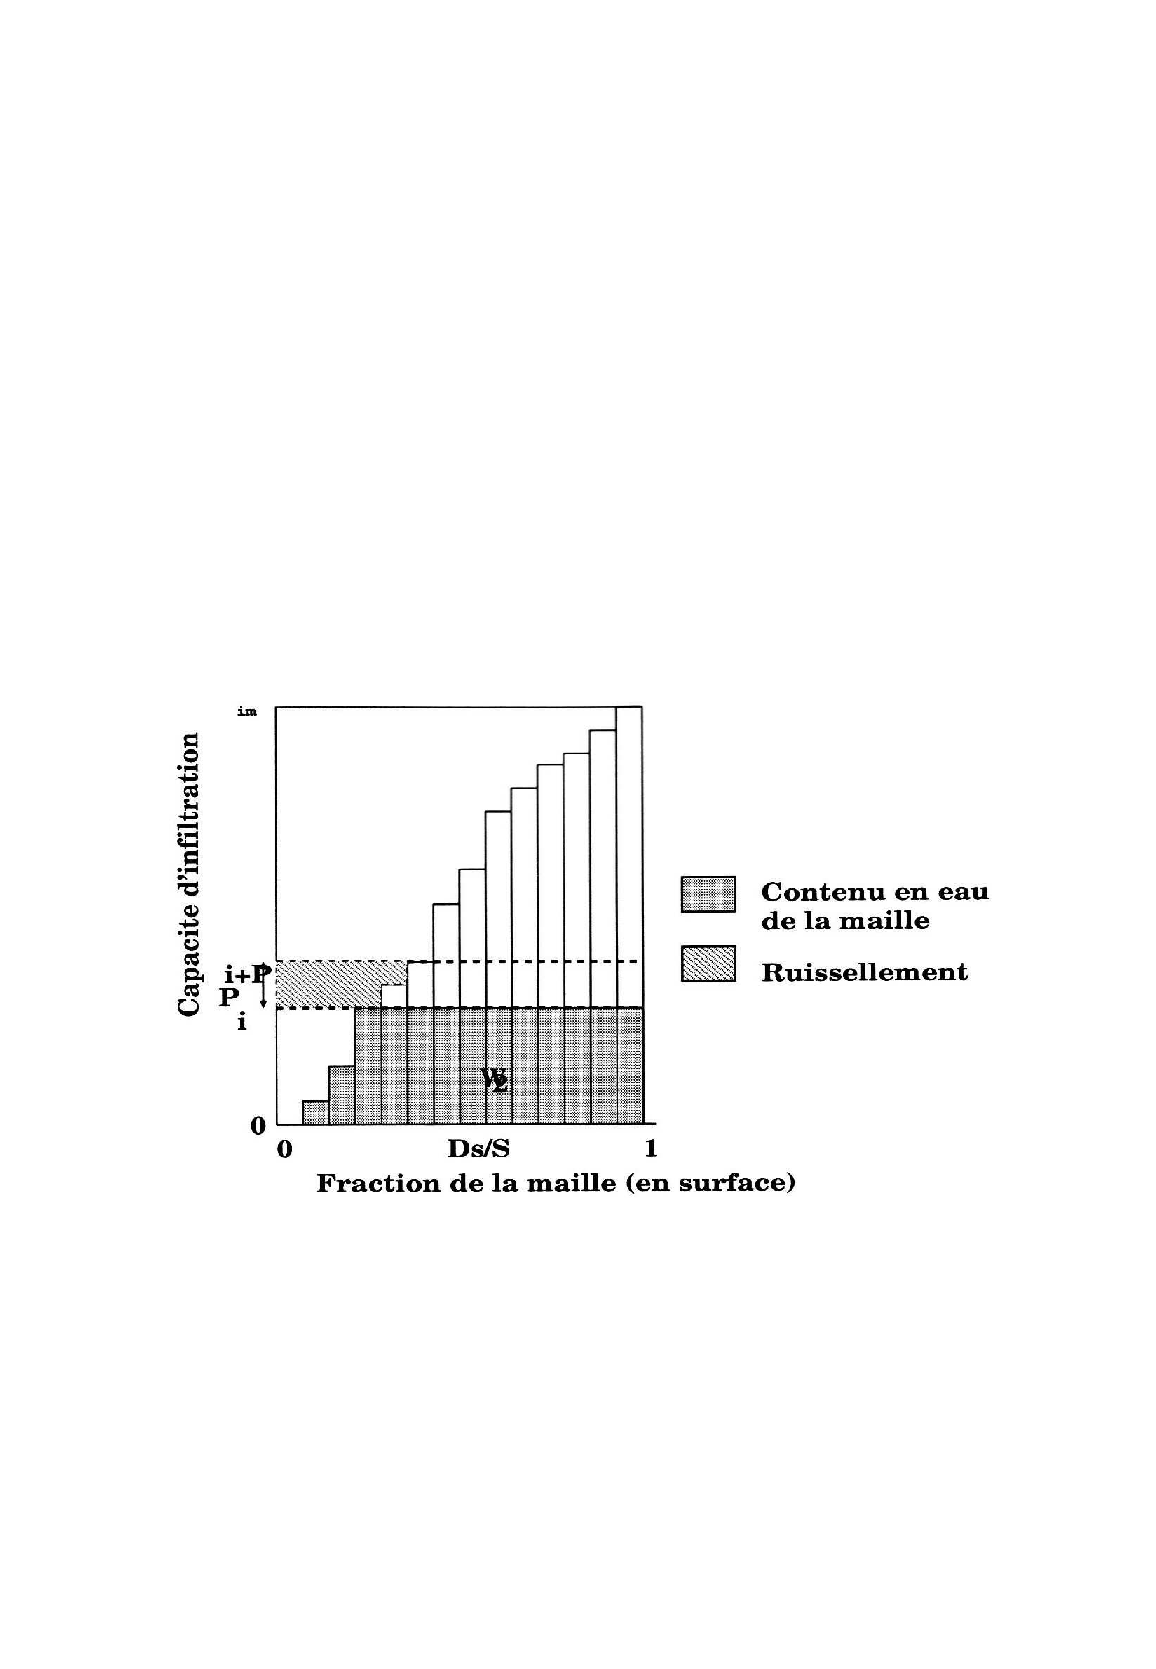
\includegraphics[angle=0, width=12cm, clip=true, trim=1cm 5cm 1cm 7cm]{EPS/ruisa.eps}
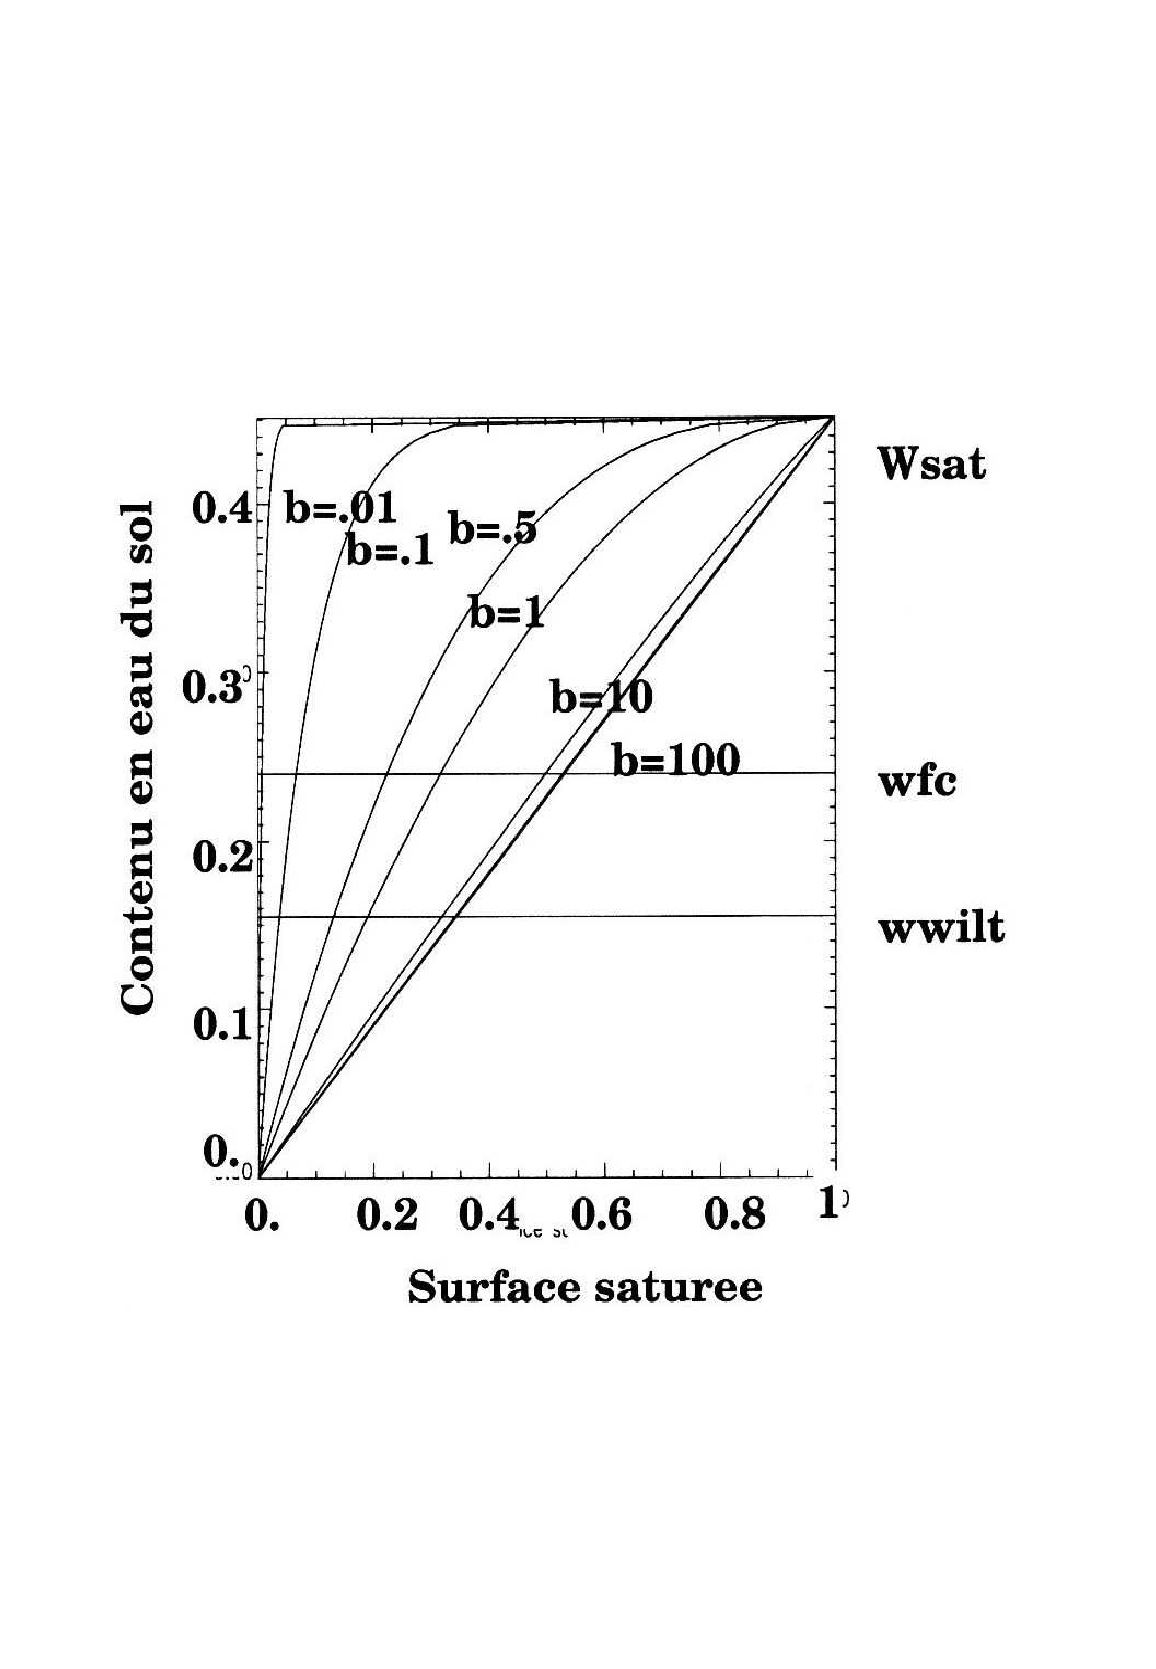
\includegraphics[angle=0, width=7cm,  clip=true, trim=1.5cm 1cm 0cm 4cm]{EPS/ruisb.eps}}
\caption{
Simplified scheme of the VIC subgrid runoff.
Left : principles. Right : variation of the saturated proportion of
the grid cell for several values of the soil water content and of the
parameter b in the VIC model. In Isba, the saturated fraction of the
grid is computed between $w_{wilt}$ and $w_{sat}$.
}
\label{fig:vic}
\end{figure}
%%%%%%%%%%%%%%%%%%%%%%%%%%%%%%%%%%%%%%

$i$ is the water content of the non saturated elementary reservoirs (all reservoirs
with a water content below $i$ are saturated). $A(i)$ is the saturated fraction of the cell.
In case of precipitation ($P$), all reservoirs with an infiltration capacity lower than $i + P$
will be filled, and then produce runoff. The runoff is the sum of the contribution of the elementary reservoirs.

In this scheme, the infiltration capacity is given by : 
%
%%%%%%%%%%%%%%%%%%%%%%%%%%%%%%%%%%%%%%%
\begin{equation}
\label{eq:i_m_vic_model}
  i=i_m \left[ 1- (1-A(i))^{\frac{1}{{\rm b}}} \right]  \Longleftrightarrow A(i)=1- \left( 1- \frac{i_0}{i_m}\right)^{\rm b}
\end{equation}
%%%%%%%%%%%%%%%%%%%%%%%%%%%%%%%%%%%%%%%
%
where $A(i)$ is the fraction of the grid cell whose the infiltration capacity is
lower than $i$ ($0 \le A(i) \le 1$), $i_m$ is the
maximum infiltration capacity of the grid cell, and b is the curvature
parameter, which controls the distribution function $A$~:
the runoff is high when b is high, and low when b is small. 

In the grid cell, the runoff is given by :
%
%%%%%%%%%%%%%%%%%%%%%%%%%%%%%%%%%%%%%%%
\begin{equation}
  Q_r = \int_{i}^{i+P} A(i) di = P + \frac{i_m}{b+1} \left[  \left( 1-
      \frac{i+P}{i_m} \right)^{{\rm b}+1} - \left( 1- \frac{i}{i_m}
    \right)^{{\rm b}+1} \right]
\end{equation}
%%%%%%%%%%%%%%%%%%%%%%%%%%%%%%%%%%%%%%%
%
For a water content $w_2$, the saturated fraction of the grid cell (
$A(w_2)$) is given by:
%
%%%%%%%%%%%%%%%%%%%%%%%%%%%%%%%%%%%%%%%
\begin{equation}
\label{eq:a_vic_model}
  A(w_2) = 1 - \left( 1 - \frac{w_2}{w_{sat}} \right)^{\frac{{\rm b}}{{\rm b}+1}}
\end{equation}
%%%%%%%%%%%%%%%%%%%%%%%%%%%%%%%%%%%%%%%
%
After preliminary testing of this parameterization on the Adour watershed, Habets \etal (1999)
found that the parameterization generated too much runoff in summer for dry
soil conditions. To avoid this problem, a threshold was introduced in
the soil wetness, $w_{c,min}$,
below which runoff was not produced. This threshold was set to be the wilting point
($w_{c,min}=w_{wilt}$). Note that this threshold is somewhat arbitrary in terms
of it's relationship to surface runoff. For example, a recent study
using ISBA has shown
that for a tropical catchment the relationship with wilting point is
weak
and a larger threshold value of $w_{c,min}$ produces
optimal results (Getirana et al., 2014\nocite{getirana_ea_2014}). So, $w_{c,min}=w_{wilt}$ should be
used by default, but a different value could be best for a given
catchment or climate (Note, currently $=w_{wilt}$ is hard-coded).


The discretized form of $Q_r$ used within the model can be written as
%
%
%%%%%%%%%%%%%%%%%%%%%%%%%%%%%%%%%%%%%%%%%%%%%%%%%%%%
\begin{subequations}
\begin{align}
\label{qrc}
Q_{r\,{\rm crit}} \,\,=\,\, &
{\left[1 - {\left(w_2-w_{c,min}\right)\over 
\left(w_{sat}-w_{c,min}\right)}\right]}^{1/(1+{\rm b})}
\,-\,
{R_t \Delta t \over \rho_w z_r}
\left[{ 1\over
(1+{\rm b})\left(w_{sat}-w_{c,min}\right)
}\right]
\\
\label{qr}
Q_r \,\,=\,\, & R_t - {\rho_w z_r \over\Delta t}
\Biggr\lbrace
\left(w_{sat}-w_2\right)-
\left(w_{sat}-w_{c,min}\right) 
{\left[{\rm max}\left(0,\,Q_{r\,{\rm crit}}\right)\right]}^{1+{\rm b}}
\Biggr\rbrace
\end{align}
\end{subequations}
%%%%%%%%%%%%%%%%%%%%%%%%%%%%%%%%%%%%%%%%%%%%%%%%%%%%
%
with the constraints:
%
%%%%%%%%%%%%%%%%%%%%%%%%%%%%%%%%%%%%%%%%%%%%%%%%%%%%%%%%
\begin{equation}
\label{qrz}
Q_r \,\,=\,\, 0
\hskip.5in
{\rm if}\hskip.2in
\left(Q_r < 0 \right) 
\hskip.2in {\rm or}\hskip.2in 
\left(w_2 \leq w_{c,min}\right) 
\end{equation}
%%%%%%%%%%%%%%%%%%%%%%%%%%%%%%%%%%%%%%%%%%%%%%%%%%%%%%%%
%
where $R_t$
(m s$^{−1}$) is the through-fall rate (sum of canopy drip, precipitation
and snow-melt). 

\paragraph{TOPMODEL approach}    TOPMODEL (TOPography based MODEL) attempted to combine the important 
distributed effects of channel network topology and dynamic contributing areas for runoff 
generation (Beven and Kirkby (1979)\nocite{beven1979}, Silvapalan \etal (1987)\nocite{Silvapalan1987}). This formalism takes into account 
topographic heterogeneities explicitly by using the spatial distribution of the topographic 
indices, $\lambda_i (m)$, in each grid-cell defined as follows:
%
\begin{equation}
  \lambda_i = \ln\left(a_i / \tan\beta_i \right) 
\end{equation}
%
where $a_i (m)$ is the drainage area per unit of contour of a local pixel, $i$, and $\tan\beta_i$ approximates 
the local hydraulic gradient where $\beta_i$ is the local surface slope. If the pixel has a large drainage 
area and a low local slope, its topographic index will be large and thus, its ability to be 
saturated will be high. Then, this topographic index can be related to a local water deficit, and 
using the spatial distribution of the topographic indices over the grid cell, a saturated fraction, 
$f_{sat}$, inversely proportional to the grid cell mean deficit, $D_t (m)$, can be defined. The 
"coupling" between TOPMODEL and ISBA was proposed by Habets and Saulnier (2001)\nocite{Habets2001} and 
generalized by Decharme \etal (2006).
The active layer used for the ISBA-TOPMODEL coupling is the rooting layer, and not 
the total soil column. TOPMODEL describes generally the evolution of a water storage deficit 
near the soil surface that reacts quasi-instantaneously following rainy events 
(Beven and Kirkby, 1979). In that case, the root zone appears to be a reasonable compromise in ISBA. So, 
the relation between the grid cell mean deficit and the soil moisture computed by ISBA is 
simply expressed as:
%
\begin{equation}
  0 \leq D_t = \left(w_{sat} - w_2 \right) \times d_2 \leq d_0 
\end{equation}
%
where $d_2 (m)$ is the rooting depth and $d_0 (m)$ the maximum deficit computed as the difference 
between the saturation, $w_sat$, and the wilting point, $w_wilt$ :
%
\begin{equation}
  d_0= \left(w_{sat} - w_{wilt} \right) \times d_2
\end{equation}

So for a given rooting soil moisture, $w_2$, a mean deficit, $D_t$, is calculated and it is therefore 
possible to determine the saturated fraction of the grid-cell. The runoff, $Q_{top}$, is thus simply 
given by: $Q_{top} = P_g \times f_{sat}$  where $P_g$ is the throughfall rain rate. For $w_2$ lower than the wilting point, 
the mean deficit is a maximum, $D_t = d_0$ , $f_{sat} = 0$ and no surface runoff occurs. Note that, the 
spatial distribution of the topographic index in each grid-cell can be computed with the three-
parameter gamma distribution introduced by Silvapalan \etal (1987)\nocite{Silvapalan1987}. The three parameters 
are derived from the mean, standard deviation, and skewness of the actual distribution that 
can be done by the HYDRO1K dataset at a 1 km resolution or another database. This 
TOPMODEL approach has been intensively validated both at the regional and global scale 
(Decharme \etal (2006), Decharme and Douville (2006 and 2007)\nocite{Decharme2006a, Decharme2007}).

\paragraph{Horton runoff approach.}   The Horton runoff 
occurs for a rainfall intensity that exceeds the effective maximum infiltration capacity. This 
infiltration excess mechanism tends to dominate the overland flow production in most desert 
or semiarid regions where short rainfall events can be very intense, but also where the absence 
of vegetation and other organic matter prevents the development of a porous soil structure 
through which water can move easily. The development of a thin crust at the soil surface can 
also inhibit the infiltration (arid or frozen soil). So the Horton runoff, $Q_{hort}$, is calculated using 
two infiltration functions following Decharme and Douville (2006): 
%
%%%%%%%%%%%%%%%%%%%%%%%%%%%%%%%%%%%%%%%%%%%%%%%%%
\begin{equation}
		  Q_{hort} = \left(1-\delta_f \right) \times \max\left(0,S_m+ P_g -I_{unf} \right)
                             + \delta_f \max \left(0,S_m+P_g -I_f \right)
\end{equation}
%%%%%%%%%%%%%%%%%%%%%%%%%%%%%%%%%%%%%%%%%%%%%%%%%
%
where $S_m$ is snowmelt, $P_g$ the throughfall rain rate, $I_{unf}$ and $I_f$ the infiltration functions over 
unfrozen and frozen soil, and $\delta_f$ the fraction of the frozen soil. These functions depend on root 
zone soil moisture conditions as well as on soil hydraulic properties. When the Horton runoff (being 
estimated only on the non-saturated fraction of the grid) is activated with the VIC or the TOPMODEL 
runoff, the surface runoff is given by :
%
\begin{equation}
  Q_s = Q_{top\_or\_vic} + \left(1-f_{sat}\right) Q_{hort}
\end{equation}

\paragraph{Treatment of drainage}

The gravitational drainage when $w > w_{fc}$ is given by the following equations 
(Mahfouf and Noilhan, 1996; Boone \etal 1999) :
%
\begin{eqnarray}
  K_2= & \frac{C_3}{\tau}\frac{d_3}{d_2} \mathrm{max}[0,(w_2 - w_{fc})] \\
  K_3= & \frac{C_3}{\tau}\frac{d_3}{d_3 - d_2} \mathrm{max}[0,(w_3 - w_{fc})] 
\end{eqnarray}
%
where $\tau$ is a characteristic time (one day).
$C_3$ is the \emph{force-restore} parameter which account for the speed
at which the humidity profile is restored to the field capacity. This
parameter depends on the hydraulic properties of the soil
(Noilhan and Mahfouf, 1996). 
In ISBA, it can be described by an empirical equation and depends on the proportion of 
clay in the grid cell.
%
\begin{equation}
  C_3 = 5.327 \cdot X^{-1.043}_{clay}
\end{equation}

%\paragraph{Subgrid drainage}    
%	 In the original formulation, the drainage stops below the field capacity $w_{fc}$.
%	 Within the framework of the Safran-Isba-Modcou model Habets \etal (2008)\nocite{Habets2008}
%         a subgrid drainage was introduced in order to account for unresolved aquifers
%	 in the model. A residual drainage was introduced in ISBA. The equations above
%	 are slightly modified :
%	 \begin{eqnarray}
%		 K_2= & \frac{C_3}{\tau}\frac{d_3}{d_2} \mathrm{max}[{w_d}_2,(w_2 - w_{fc})] \\
%		 K_3= & \frac{C_3}{\tau}\frac{d_3}{d_3 - d_2} \mathrm{max}[{w_d}_3,(w_3 - w_{fc})] 
%	 \end{eqnarray}
%
%	 In this formulation, ${w_d}_i$ (for each layer $i$) is expressed as :
%    \begin{equation}
%    	{w_d}_i = w_{drain} max \left( 0, \frac{ min(w_{fc},w_i) - {w_g}_{min}} {w_{fc}-{w_g}_{min}} \right) 
%     \end{equation}
%
%	 where $w_{drain}$ is a parameter to be calibrated, and ${w_g}_{min}$ 
%	 a small parameter to avoid numerical problems.
%
%	 $w_{drain}$ must be calibrated using discharge measurements
%	 during dry periods. See Caballero \etal
%	 (2007)\nocite{Caballero2007},
%
%	 and Habets \etal (2008) for calibration with discharge for the Safran-Isba-Modcou model.


%=========================================================================================================
\subsubsection{Treatment of soil ice}
\label{sec:isba_soil_ice_treatment}
%=========================================================================================================

The inclusion of soil freezing necessitates the addition
of so-called phase change to the thermal and hydrological
transfer equations. In addition,
a freezing/drying wetting/thawing analogy is
used to model changes in the force-restore coefficients
so that they must also be modified accordingly. Terms which have been
added to the baseline ISBA scheme are underlined in this
section, while terms which are modified are denoted using
an $\ast$ superscript.
Additional details related to soil freezing scheme 
can be found in Boone \etal (2000) and Boone (2000)\nocite{Boone2000a}.

The basic prognostic equations
including soil ice are expressed as
%
\begin{eqnarray}
\frac{\partial T_s}{\partial t} &=&
{C_T}^\ast \left[ R_n \,-\, H \,-\, {LE}^\ast \,-\,
L_f(M_s-{\underline{F_{g\,w}}})\right] \,-\,
\frac{2\pi}{\tau}(T_s-T_2)
\,\,\,, \\
%
\frac{\partial T_2}{\partial t} &=&
\frac{1}{\tau}(T_s-T_2)
\,+\,{C_G}^\ast L_f {\underline{F_{2\,w}}}
\,\,\,, \\
%
\frac{\partial w_g}{\partial t} &=&
\frac{1}{ d_1\rho_w} \left[ {C_1}^\ast\left(P_g-E_{g\,l}+M_s \right)
\,-\, {\underline{F_{g\,w}}} \right]
\,-\, \frac{{C_2}^\ast}{\tau}(w_g-{w_{g\,{\rm eq}}}^\ast) \\
& & \hskip2.6in
(w_{{\rm min}} \leq w_g \leq w_{\rm sat}-w_{g\,f})
\,\,\,, \\
%
\frac{\partial w_2}{\partial t} &=&
\frac{1}{ d_p\rho_w}
\left(P_g-{E_{g\,l}}-{E_{tr}}^\ast+M_s-
{\underline{F_{2\,w}}} \right) \,-\,{C_3}{\tau}{\rm max}
(0\,,\,\,w_2-{w_{\rm fc}}^\ast) \\
& & \hskip2.6in
(w_{{\rm min}}\leq w_2 \leq w_{\rm sat}-w_{2\,f})
\,\,\,, \\
%
\frac{\partial w_{g\,f}}{\partial t} &=&
\frac{1}{ d_1 \rho_w} \left(
F_{g\,w} \,-\, E_{g\,f} \right)
\hskip1.35in
(0 \leq w_{g\,f}\leq w_{\rm sat}-w_{{\rm min}} )
\,\,\,, \\
%
\frac{\partial w_{2\,f}}{\partial t} &=&
\frac{1}{ \left(d_2-d_1\right)\rho_w} F_{2\,w}
\hskip1.6in
(0 \leq w_{2\,f}\leq w_{\rm sat}-w_{{\rm min}} )
\,\,\,.
\end{eqnarray}
%
where $w_{g\,f}$ and $w_{2\,f}$ represent the volumetric soil ice content
(m$^3$ m$^{-3}$) in the surface and deep-soil reservoirs, respectively.
The phase change mass and heat sink (source) terms ($F$; kg m$^{-2}$ s$^{-1}$)
are expressed as
%
\begin{eqnarray}
F_{g\,w} &=& \left(1-p_{sng}\right)\,\left( F_{g\,f}
\,-\, F_{g\,m}\right)\,\,\,, \\
%
F_{2\,w} &=& \left(1-p_{sng}\right)\,\left( F_{2\,f}
\,-\, F_{2\,m}\right)\,\,\,,
\end{eqnarray}
%
where the $m$ and $f$ subscripts represent melting and
freezing, respectively.
The freezing and melting phase change terms are formulated using simple
relationships based on the potential
energy available for phase change. They are expressed
for the surface soil layer as
%
\begin{eqnarray}
F_{g\,f} &=& \left(1/\tau_i \right)\,{\rm min} \left[
K_s \,\epsilon_{s\,f} \,{\rm max}(0,\,T_0-T_s)/C_I \, L_f ,\,
\rho_w\,d_1\,\left( w_g-w_{\rm min} \right)
\right]
\,\,\, , \\
%
F_{g\,m} &=& \left(1/\tau_i \right)\,{\rm min} \left[
K_s \,\epsilon_{s\,m} \,{\rm max}(0,\,T_s-T_0)/C_I \, L_f ,\,
\rho_w\,d_1\,w_{g\,f}
\right]
\,\,\, ,
\end{eqnarray}
%
and for the deep soil layer as
%
\begin{eqnarray}
F_{2\,f} &=& \left(\delta_{2\,f}/\tau_i \right)\,{\rm min} \left[
\epsilon_{2\,f} \,{\rm max}(0,\,T_0-T_2)/C_I \, L_f , \,
\rho_w\,\left(d_2-d_1\right)\left( w_2-w_{\rm min}\right)\right]
\,\,\, ,\\
%
F_{2\,m} &=& \left(1/\tau_i \right)\,{\rm min} \left[
\epsilon_{2\,m} \,{\rm max}(0,\,T_2-T_0)/C_I \, L_f , \,
\rho_w\,\left(d_2-d_1\right)\,w_{2\,f}\right]
\,\,\,.
\end{eqnarray}
%
The characteristic time scale for freezing is represented by $\tau_i$ (s).
The phase change efficiency coefficients, $\epsilon$, introduce
a dependence on the water mass available for phase changes
which are expressed as
the ratio of the liquid volumetric water content
to the total soil porosity for freezing,
and the ratio of ice content to the porosity for melting.
The ice thermal inertia coefficient is defined as
$C_I = 2 {\left( {\pi/\lambda_i\,C_i\rho_i\tau} \right)}^{1/2}$
(J m$^{-2}$ K$^{-1}$).
The insulating effect of vegetation is modeled using a coefficient
defined as
%
\begin{eqnarray}
K_s =
\, \left(1-\frac{veg}{ K_2}\right) \left(1-\frac{LAI}{ K_3}\right) \,\,\,,
\end{eqnarray}
%
where the dimensionless coefficients have
the values $K_2\,=\,5.0$ and $K_3\,=\,30.0$ (Giard and Bazile (2000)\nocite{Giard2000}).
The most direct
effect of vegetation cover
is to slow the rate of phase changes for more dense vegetation cover
as energy not used for phase change is assumed to cool/warm the
vegetative portion of the lumped soil-vegetation layer.

The deep-soil phase change (freezing) term
is multiplied by a factor ($\delta_{2\,f}$)
which essentially limits ice production during prolonged
cold periods.  It is defined as 0 if $z_f \geq z_{f\,{\rm max}}$
where
%
\begin{eqnarray}
z_{f\,{\rm max}} &=& 4/\left( {C_G}^\ast\,c_g\right)
\,\,\,
\end{eqnarray}
and the actual depth of ice in the soil is defined as
\begin{eqnarray}
z_f &=& d_2 \, \left(\frac{w_{2\,f}}{ w_{2\,f} + w_2}\right)
\hskip1.in \left(0 \leq z_f < d_2\right)
\end{eqnarray}
%
Ice is assumed to become
part of the solid soil matrix. This is accomplished by
defining the modified porosity
(eg. Johnsson and Lundin (1991)\nocite{Johnsson1991}) as
%
\begin{eqnarray}
{w_{sat}}^\ast = w_{sat} - w_{j\,f}
\end{eqnarray}
%
where $j$ corresponds to the surface ($g$) or sub-surface ($2$)
soil water reservoirs.
This, in turn, is used to modify the force-restore coefficients
(see Boone \etal, 2000, for more details).

As a final note, more recently an option to this simple method to
compute the phase changes has been
added based on the Gibbs-free energy approach. It is especially
adapted for the DuFfusion (DF) version of ISBA (see
Section~\ref{sec:isba_diffusion_soil}), but it can also be used with
the FR approach. See Section~\ref{sec:isba_soil_ice} for more details.
But the soil ice modification to the porosity etc. remains as described
in this Section for both phase change options.

%=========================================================================================================
%=========================================================================================================
\subsection{Diffusive approach}
\label{sec:isba_diffusion_soil}
%=========================================================================================================
%=========================================================================================================

%
%=========================================================================================================
\subsubsection{Governing Equations}
%=========================================================================================================
%
The governing equations for the heat and mass transfer
from the surface down through the soil column for the snow-free
case are expressed as (Boone \etal 2000; Decharme \etal 2011):
%
\begin{eqnarray}
c_h\frac{\partial T_g}{ \partial t } \,\,&=&\,\,
\frac{\partial G }{ \partial z} 
\,+\,\Phi \label{tdifsn} \\
%
\frac{\partial w_l }{\partial t} \,\,&=&\,\,
-\frac{\partial F}{\partial z} \,-\, \frac{\Phi}{ L_f \rho_w}\,-\, \frac{S_l}{ \rho_w}
\hskip.8in (w_{min}\,\leq\, w_l\,\leq\,w_{sat}-w_i) \label{cont1}\\
%
\frac{\partial w_i}{\partial t} \,\,&=&\,\,
\frac{\Phi}{ L_f \rho_w} \,-\, \frac{S_i}{ \rho_w}
\hskip1.32in (0 \,\leq\, w_i\,\leq\,w_{sat}-w_{min})\label{ice} 
\end {eqnarray}
%
Eq.~(\ref{tdifsn}) is the vertical component of the 
heat transfer equation: heat flow is induced
along the thermal gradient and due to convection,
$c_h$ is the total heat capacity
(J ${\rm m^{-3}\,K^{-1}}$): it is represented by
a lumped heat capacity in the surface layer, and by
the soil heat capacity ($c_g$) in the sub-surface layers.
$\lambda$ is the thermal conductivity (W ${\rm m^{-1}\,K^{-1}}$),
$F$ is the vertical flow rate of water (m ${\rm s^{-1}}$),
$T_g$ is the composite soil-vegetation  temperature (K) at the surface
and the soil temperature only for sub-surface layers, $\Phi$ (${\rm J \, m^{-3}\,s^{-1}}$)
is a latent heat
source/sink resulting from phase transformation of soil water,
and the soil depth, $z$ (m), is increasing downward.

$w_l$ and $w_i$ in Eq.s~(\ref{cont1}) and (\ref{ice}) 
represent
the volumetric liquid water and liquid water equivalent ice contents
of the soil (${\rm m^3 \, m^{-3}}$), respectively. They are
related to the total volumetric water content 
(${\rm m^3 \,m^{-3}}$) through
%
\begin{equation} \label{totalsoilwater}
w \,\,=\,\,w_l \, +\, w_i
\,\,\, .
\end{equation}
%
In Eq.~(\ref{cont1}), 
$S_l$ (evapotranspiration, lateral inflow) 
and $S_i$ (sublimation) represent external sources/sinks
(kg m$^{-3}$ s${-1}$), 
of the liquid and ice liquid equivalent soil water, respectively, 
$L_f$ is the latent heat of fusion 
(3.337 ${\rm \times {10}^5 \,J\,{kg}^{-1}}$),
and $\rho_w$ is the density
of liquid water (1000 kg ${\rm m^{-3}}$).
The total soil porosity is 
$w_{sat}$ (${\rm m^3 \, m^{-3}}$), and
$w_{min}$ is a minimum liquid water threshold
(0.001 ${\rm m^3 \, m^{-3}}$).

The phase change terms on the right-hand sides of Eq.s~(\ref{cont1}) 
and (\ref{ice}) represent a mass
transfer between the solid and liquid phases
of the soil water. 
The continuity equation for the total
soil volumetric water content is obtained by
adding Eq.s~(\ref{cont1}) and (\ref{ice}) and then
substituting Eq.~(\ref{totalsoilwater}) 
into the resulting expression to have
%
%%%%%%%%%%%%%%%%%%%%%%%%%%%%%%%%%%%%%%%%%%%%%%%%%%%%%%%%
\begin{equation}
%\label{}
\frac{\partial w}{\partial t} \,\,=\,\,
-\frac{\partial F}{\partial z} \,-\, \frac{1}{\rho_w}\left(S_i\,+\, S_l\right)
\hskip.8in 
\left(w_{min}\,\leq\, w\,\leq\,w_{sat}\right)
\end{equation}
%%%%%%%%%%%%%%%%%%%%%%%%%%%%%%%%%%%%%%%%%%%%%%%%%%%%%%%%
%

%=========================================================================================================
\subsubsection{Surface and soil heat transfer}
%=========================================================================================================
%
Heat flow is along the thermal gradient,
so that the soil heat flux (W m$^{-2}$) can be expressed as
%
%%%%%%%%%%%%%%%%%%%%%%%%%%%%%%%%%%%%%%%%%%%%%%%%%%%%%%%%
\begin{equation}
\label{gxxx}
G = \lambda \frac{\partial T}{\partial z}
\end{equation}
%%%%%%%%%%%%%%%%%%%%%%%%%%%%%%%%%%%%%%%%%%%%%%%%%%%%%%%%
%
The soil thermal conductivity and heat capacity 
are expression as functions of soil properties
and moisture. The parameterizations are described below.

\paragraph{Calculation of the thermal properties}
%
The thermal heat capacity and thermal conductivity
are parameterized as functions
of the soil moisture and texture by most SVAT schemes.
SVAT schemes which participated in
PILPS-phase2c predicted, in general, ground heat fluxes
poorly, which is most likely related to thermal 
conductivity parameterization Liang \etal (1996)\nocite{Liang1996}. 
ISBA uses the formulations from McCumber and Pielke (1981 : MP81)\nocite{McCumber1981}
together with parameter values from Clapp and Hornberger (1978)
to evaluate the heat capacity and thermal conductivity
(Noilhan and Planton, 1989), but
it is known that thermal conductivity estimates using the 
MP81 model tend to be too large for wet conditions (nearing saturation)
while underestimating thermal conductivity for dry soils.
Also, there is no consideration of frozen soils in this formulation.
There are several alternatives to using the MP81 
model for thermal conductivity, and
one such method is that discussed in Peters-Lidard \etal (1998)\nocite{Peters-Lidard1998}.
%
The layer-averaged soil heat capacity can be written as
%
\begin{equation}\label{heatcapacity}
c_{g\,j} \,\,=\,\, (1-w_{sat})C_{soil}\rho_{soil} 
\,+\, w_{l\,j} c_w \, +\, w_{i\,j} c_i 
\end{equation}
%
where 
$c_i$ and $c_w$ are the heat capacities of ice and liquid water, 
(J ${\rm K^{-1} \, m^{-3}}$).
$C_{soil}$ is the specific heat of the soil (J ${\rm {kg}^{-1}}
\, K^{-1}$) and $\rho_{soil}$ represents the soil dry density.
The specific heat ($C_{soil}$) value of 733 J ${\rm {kg}^{-1} \, K^{-1}}$
for soil minerals/quartz from
Peters-Lidard \etal (1998) is used.
%The dry density is sometimes measured, but it can also be
%estimated from the soil porosity assuming the same solids unit
%weight (Peters-Lidard \etal 1998):
%
%%%%%%%%%%%%%%%%%%%%%%%%%%%%%%%%%%%%%%%%%%%%%%%%%%%%%%%%
%\begin{equation}
%\rho_{soil} \,\,=\,\, (1-w_{sat})\rho_{solids} 
%\end{equation}
%%%%%%%%%%%%%%%%%%%%%%%%%%%%%%%%%%%%%%%%%%%%%%%%%%%%%%%%
%
where $\rho_{soil}$ represents the unit weight of the solids 
(2700 kg ${\rm m^3}$).
%
The heat capacity of air in the soil is neglected in
Eq.~(\ref{heatcapacity}).

For fine soils or coarse frozen soils, the method of Johansen (1975)\nocite{johansen1975} was 
shown by Farouki (1986)\nocite{farouki1986} to be the most accurate relative to other commonly
used methods for calculating thermal conductivity.
Following Peters-Lidard \etal (1998),
the thermal conductivity is calculated as the weighted sum of
the dry and saturated thermal conductivities from (Johansen, 1975)
%
\begin{equation}\label{condpl}
\lambda \,\,=\,\, K_e \,\lambda_{sat} \,+\,(1-K_e)\,\lambda_{dry}
\end{equation}
%
where $K_e$ is the non-dimensional Kersten number.

The dry thermal conductivity is defined as
%
%%%%%%%%%%%%%%%%%%%%%%%%%%%%%%%%%%%%%%%%%%%%%%%%%%%%%%%%
\begin{equation}
\label{conddry}
\lambda_{dry} \,\,=\,\, 
\frac{0.135 \rho_{soil} \,+\,64.7}
{\rho_{solids} \,-\,0.947 \rho_{soil}}
\end{equation}
%%%%%%%%%%%%%%%%%%%%%%%%%%%%%%%%%%%%%%%%%%%%%%%%%%%%%%%%
%
where $\lambda_{dry}$ is in W ${\rm m^{-1}}\, K^{-1}$.
%
For crushed rock, 
%
%
%%%%%%%%%%%%%%%%%%%%%%%%%%%%%%%%%%%%%%%%%%%%%%%%%%%%%%%%
\begin{equation}
\lambda_{dry} \,\,=\,\, 0.039 \, {w_{sat}}^{-2.2}
\end{equation}
%%%%%%%%%%%%%%%%%%%%%%%%%%%%%%%%%%%%%%%%%%%%%%%%%%%%%%%%
%
The saturated thermal conductivity is written as
%
\begin{equation}\label{condsat}
\lambda_{sat} \,\,=\,\, 
{\lambda_{soil}}^{(1-w_{sat})}\,
{\lambda_{i}}^{(w_{sat}-\chi_u)}\,
{\lambda_{w}}^{\chi_u}
\end{equation}
%
where $\chi_u$ represents the unfrozen volume fraction of the soil.
It is defined as
%
%
%%%%%%%%%%%%%%%%%%%%%%%%%%%%%%%%%%%%%%%%%%%%%%%%%%%%%%%%
\begin{equation}
\chi_u \,\,=\,\,w_{sat}\left(w_l/w\right)
\hskip.5in
\left(0 \,\leq\,\chi_u \,\leq\,w_{sat}\right)
\end{equation}
%%%%%%%%%%%%%%%%%%%%%%%%%%%%%%%%%%%%%%%%%%%%%%%%%%%%%%%%
%
%
In Eq.~(\ref{condsat}),
$\lambda_{i}$ represents the thermal conductivity of ice
(2.2 W ${m^{-1}\,K}$), $\lambda_{w}$ represents the thermal 
conductivity of water
(0.57 W ${m^{-1}\,K}$), and
the thermal conductivity of solids is written as
%
%
%%%%%%%%%%%%%%%%%%%%%%%%%%%%%%%%%%%%%%%%%%%%%%%%%%%%%%%%
\begin{equation}
\label{condsolids}
\lambda_{soil} \,\,=\,\, {\lambda_q}^q \,{\lambda_o}^{1-q}
\end{equation}
%%%%%%%%%%%%%%%%%%%%%%%%%%%%%%%%%%%%%%%%%%%%%%%%%%%%%%%%
%
%
The quartz content ($0 \leq q \leq 1$) is non-dimensional.
It is fit as a function of sand (following the method of
Noilhan and Lacarr\`{e}re (1995)\nocite{Noilhan1995}
using the data from PL98:
%
\begin{equation}\label{quartzr}
q \,\,=\,\, 0.038 \,+\, 0.0095 \,X_{\rm sand} 
\end{equation}
%
where the fraction of the soil comprised by sand
is represented by $X_{\rm sand}$ (\%). The relation is
shown graphically in Fig.~(\ref{quartzf}).
The thermal conductivity of quartz is represented as
$\lambda_q$ (7.7 W ${m^{-1}\,K}$), and 
the thermal conductivity of other minerals is represented as
$\lambda_o$ (W ${m^{-1}\,K}$) where
%
%%%%%%%%%%%%%%%%%%%%%%%%%%%%%%
\begin{equation}
%
\lambda_o \,\, = \,\, \Bigg\lbrace
%
\begin{matrix}
2 & q > 0.2
\\
3 & q \leq 0.2
%
\end{matrix}
%
\end{equation}
%%%%%%%%%%%%%%%%%%%%%%%%%%%%%%
%
\begin{figure}[h]
		 \begin{center}
		 \psfig{figure=EPS/quartz.eps,width=8cm}
		 \caption{The relation between quartz content ($q$) and
sand fraction ($X_{\rm sand}$) of the soil (\%).
The relationship between quartz and sand content
is described by Eq.~(\ref{quartzr}).
The data are plotted using the values of $q$ from
Peters-Lidard \etal (1998) and the sand fraction
from Cosby \etal (1984).}
\label{quartzf}
		 \end{center}
\end{figure}
\nocite{Cosby1984}


The Kersten number is written as
%
%
%%%%%%%%%%%%%%%%%%%%%%%%%%%%%%
\begin{equation}
%
K_e \,\, = \,\, \Bigg\lbrace
%
\begin{matrix}
0.7 \, {\rm log}_{10}\,\theta \,+\,1.0 & 
\theta > 0.05 \,\, ({\rm coarse})
\\
{\rm log}_{10}\,\theta \,+\,1.0 & 
\theta > 0.10 \,\, ({\rm fine})
%
\end{matrix}
%
\end{equation}
%%%%%%%%%%%%%%%%%%%%%%%%%%%%%%
%
and for frozen soils it is
%
\begin{equation}\label{kerstfrz}
K_e = \theta 
\end{equation}
%
where $\theta$ is the degree of saturation ($w/w_{sat}$) of the soil
layer. Because use of Eq.~(\ref{kerstfrz}) can result in
a large jump in $K_e$ as a soil begins to freeze, the following expression
is used for partially frozen fine soils:
%
\begin{equation}\label{kerstfrzp}
K_e \, = \, (w_l/w)\left({\rm log}_{10}\,\theta\,+\,1.0\right)
 \,+\, (w_i/w)\theta
\end{equation}
%
The same weighting scheme in Eq.~(\ref{kerstfrzp})
can be used for coarse soils as well. 

\paragraph{Numerical discretization of the soil heat equation}
%
%Integrating the heat transfer equation [Eq.~(\ref{tdifsn})]
%downward into the soil to obtain the 
%average temperature for $N$ soil layers:
%%
%\begin{equation}\label{inttdif}
%\int_{-z_j}^{-z_{j-1}} 
%c_h 
%\frac{\partial T_g}{\partial t } dz \,\,=\,\,
%\int_{-z_j}^{-z_{j-1}} 
%%{\partial }{ \partial z} \lambda {\partial T }{ \partial z} dz
%\frac{\partial G}{\partial z} dz
%%%\,+\,\int_{-z_j}^{-z_{j-1}} {\partial (F\,T)}{\partial z} dz
%\,+\,\int_{-z_j}^{-z_{j-1}} \Phi dz
%\end{equation}
%
%where
%
%\begin{equation}\label{tavglyr}
%T_{g,\,j} \,\,=\,\, \frac{1}{\Delta z_j} \int_{-z_j}^{-z_{j-1}}
%\,T_g dz
%\end{equation}
%
%$T_{g,\,j}$ is the layer averaged temperature ($j=1,...,N$),
%the vertical index $j$ is increasing downward and
%$\Delta z_j$ is defined as $z_j - z_{j-1}$. 

%Carrying out the integration in Eq.~\ref{inttdif} using 
%the operator in Eq.~\ref{tavglyr} yields
%
The governing equations for heat transfer within the soil discretized
in $N_g$ layers are described using the classical one-dimensional Fourier
law and are written as:
%
%%%%%%%%%%%%%%%%%%%%%%%%%%%%%%%%%%%%%%ù
\begin{subequations}
\begin{align}
\label{teq}
\Delta z_j c_{g\,j}\frac{\partial T_{g,\,j}}{\partial t } \,\,=&\,\,
G_{j-1} \,-\, G_j 
\,+\,\Delta z_j\,\Phi_j
\hskip2.5in
\forall = 2,N_g
\\
\label{teq_flux}
\Delta z_j c_{g\,j}\frac{\partial T_{g,\,j}}{\partial t } \,\,=&\,\,
\frac{{\overline\lambda}_{j-1}}{\Delta {\tilde z}_{j-1}}
\left( T_{g,\,j-1} \,-\, T_{g,\,j}\right)
\,-\,
\frac{{\overline\lambda}_j}{\Delta {\tilde z}_j}
\left( T_{g,\,j} \,-\, T_{g,\,j+1}\right)
\,+\,\Delta z_j\,\Phi_j
%
\end{align}
\end{subequations}
%%%%%%%%%%%%%%%%%%%%%%%%%%%%%%%%%%%%%%ù
%
where the heat conduction flux (W m$^{-2}$) 
is therefore defined as
%
%%%%%%%%%%%%%%%%%%%%%%%%%%%%%%%%%%%%%%ù
\begin{equation}
\label{teq_flux}
G_j \,\,=\,\,
\frac{{\overline\lambda}_j}{\Delta {\tilde z}_j}
\left( T_{g,\,j} \,-\, T_{g,\,j+1}\right)
%
\end{equation}
%%%%%%%%%%%%%%%%%%%%%%%%%%%%%%%%%%%%%%ù
%
$\Delta z_j$ (m) is the thickness of the layer $j$,
$\Delta {\tilde z}_j=\left(\Delta z_j+\Delta z_{j+1}\right)/2$ 
is the thickness (m) between two consecutive layer mid-points or nodes,
$C_G$ is the soil thermal inertia at the surface (J m$^{-1}$
kg$^{-2}$),
$c_{g\,j}$ is the total soil heat capacity(J m$^{-3}$ K$^{-1}$), and
${\overline\lambda}_j$ (W m$^{-1}$ K$^{-1}$)
is the inverse-weighted arithmetic mean of the soil thermal conductivity 
at the interface between two consecutive nodes
expressed as:
%
%%%%%%%%%%%%%%%%%%%%%%%%%%%%%%%%%%%%%%%%%%%%%%%%%%
\begin{equation}\label{thckwtdif}
{\overline \lambda}_j \,\,=\,\, 
\frac{\Delta z_{j} + \Delta z_{j+1}}
{\left(\Delta z_{j+1}/\lambda_{j+1}\right) \,+\,
\left(\Delta z_{j}/\lambda_{j}\right)}
\,\,\, .
\end{equation}
%%%%%%%%%%%%%%%%%%%%%%%%%%%%%%%%%%%%%%%%%%%%%%%%%%
%
%The convective heat flow term is parameterized following 
%Pitman et al. (1991) as
%%
%$$ G_{c\,j} \,\,=\,\, 
%{2\,c_w\,F_{j-1}\left( T_j-T_{j-1}\right)
%}{ \left( \Delta z_j + \Delta z_{j-1}\right)}
%\,\,\, ,\eqno\label{heatconv}$$
%%
%using the upwind difference scheme
%where $F_{j-1}$ represents the soil water flux accross
%the level $z=z_{j-1}$. 
In general, the contribution of convective heating to the local
soil temperature change is relatively small and can be neglected.
Vapor transfer effects have been incorporated and are currently
being tested: they are not outlined here.
%This term is retained in this formulation, however, as it could
%become important for cases such as the warming of soil
%due to the infiltration of snow melt.
%Note that the values of thermal conductivity and heat
%capacity are held constant over the time step, which is
%a reasonable approximation as long as time steps are not
%too large. 
The model grid configuration is shown in Fig.~\ref{grid}.
The shaded region at the surface represents a vegetation/biomass/litter
layer. The prognostic variables ($T_{g,\,j}$, $w_l$, and $w_i$) 
are shown (water store variables
will be discussed in subsequent sections).

\begin{figure}[h]
		 \begin{center}
		 \psfig{figure=EPS/tgrid_new.ps,width=10cm}
		 \caption{The model grid configuration: soil prognostic variables
temperature ($T_{g,\,j}$), liquid volumetric water content
($w_{l\,j}$) and volumetric ice content ($w_{i\,j}$) 
are layer mean quantities. The soil heat ($G_j$) and liquid
water fluxes ($F_j$) are evaluated at each level, $z_j$.
The surface energy budget is evaluated defining $T_s = T_{g,\,1}$.
The shaded region at the surface represents a vegetation/biomass/litter.
The soil depth, $z$, is increasing downward (away from the atmosphere).}
		 \label{grid}
		 \end{center}
\end{figure}


\paragraph{Boundary conditions}


Upper boundary condition: 
%
To be consistent with the ISBA-FR surface energy budget, the surface
temperature evolves according to the heat storage in the
soil/vegetation composite and to the thermal gradient between the
surface (the same fine superficial layer than for ISBA-FR) and the
second layer (Boone \etal ,2000\nocite{Boone2000}).
Accordingly, the surface temperature is defined as
%
%%%%%%%%%%%%%%%%%%%%%%%%%%%%%%%%%%%%%%%%%%%%%%%%%%
\begin{subequations}
\begin{align}
%
\label{eq:tsfc}
\frac{1}{C_T} \frac{\partial T_{g,1}}{\partial t} \,\,=&\,\,
G_0 \,+\, \Delta z_1 \,\Phi_1 \,-\, \frac{C_G}{C_T}
\frac{{\overline\lambda}_1}{\Delta {\tilde z}_1}\left(
  T_{g,1} - T_{g,2}\right) \\
%
\label{eq:tsfc_b}
\frac{\partial T_{g,1}}{\partial t} \,\,=&\,\,
C_T \left( R_n \,-\, H \,-\, LE \,+\, \Delta z_1 \,\Phi_1 \right) \,-\, 
C_G \, \frac{{\overline\lambda}_1}{\Delta {\tilde z}_1}
\left( T_{g,1} - T_{g,2}\right) 
%
\end{align}
\end{subequations}
%%%%%%%%%%%%%%%%%%%%%%%%%%%%%%%%%%%%%%%%%%%%%%%%%%
%
where the
flux between the atmosphere and the surface
is represented by $G_0$ (W m$^{-2}$).
This definition of the prognostic equation for $T_{g,1}$
is similar to that presented by
Bhumralkar (1975)\nocite{Bhumralkar1975} and Blackadar (1979)\nocite{Blackadar1976}. It is the same as
the standard Force-Restore method of Noilhan and Planton (1989)\nocite{Noilhan1989}
if $G_1$ is expressed as a restore term.
The thermal inertia coefficient for the composite surface
layer is expressed as
%
%
%%%%%%%%%%%%%%%%%%%%%%%%%%%%%%%%%%%%%%%%%%%%%%%%%%%%%%%%
\begin{equation}
C_T = {\frac{1}{\left(veg/C_V\right)+\left[(1-veg)/C_G\right]}}
\end{equation}
%%%%%%%%%%%%%%%%%%%%%%%%%%%%%%%%%%%%%%%%%%%%%%%%%%%%%%%%
%
%
where $veg$ represents the vegetation cover fraction.
The thermal inertia for the vegetation ($C_V$) can
be case or species dependent. By default, it is computed as
%
%%%%%%%%%%%%%%%%%%%%%%%%%%%%%%%%%%%%%%%%%%%%%%%%%%%%%%%%
\begin{equation}
C_V = \frac{1}{C_{V,ref} + c_w\,W_r}
\end{equation}
%%%%%%%%%%%%%%%%%%%%%%%%%%%%%%%%%%%%%%%%%%%%%%%%%%%%%%%%
%
where $W_r$ (kg m$^{-2}$) is the vegetation interception 
reservoir water storage
and $C_{v,ref}$ (J K$^{-1}$ m$^{-2}$) the reference or baseline
vegetation heat capacity (defined by the user or ECOCLIMAP)
set by default to $1\times 10^4$ J K$^{-1}$ m$^{-2}$ for low
vegetation 
and $2\times 10^4$ J K$^{-1}$ m$^{-2}$ for forests.
%
The soil thermal inertia (J K$^{-1}$ m$^{-2}$) is
defined as
%
%%%%%%%%%%%%%%%%%%%%%%%%%%%%%%%%%%%%%%%%%%%%%%%%%%%%%%%%
\begin{equation}
C_G = \frac{1}{c_{g,1}\,\Delta z_1}
\end{equation}
%%%%%%%%%%%%%%%%%%%%%%%%%%%%%%%%%%%%%%%%%%%%%%%%%%%%%%%%
%
where $c_{g,1}$ is the heat capacity of the first soil layer
(J K$^{-1}$ m$^{-3}$: Eq.~\ref{heatcapacity}).
The uppermost soil thickness, $\Delta z_1$, must be chosen to be sufficiently
thin in order to be consistent with the daily surface temperature
cycle (i.e., 0.01 m by default). 
%
%%%%%%%%%%%%%%%%%%%%%%%%%%%%%%%%%%%
%
%The thermal conductivity of the surface layer is represented by $\lambda_s$.
%There is an option 
%to include the effects of a vegetation/mulch/thin biomass litter
%layer using:
%
%
%%%%%%%%%%%%%%%%%%%%%%%%%%%%%%%%%%%%%%%%%%%%%%%%%%%%%%%%
%\begin{equation}
%\lambda_s = \left[ 1 - veg \left( 1-f_v \right)\right] \lambda_1 
%\end{equation}
%%%%%%%%%%%%%%%%%%%%%%%%%%%%%%%%%%%%%%%%%%%%%%%%%%%%%%%%
%
%where $f_v$ is a reduction factor for the surface layer
%thermal condictivity due to the presence of mulch or organic material.
%The value of this parameter ranges between $0 < f_v \leq 1$, depending upon the
%insulating effect of the material. Following from the ideas of Gonzalez-Sosa \etal (2001)\nocite{Gonzalez-Sosa2001},
%it is assumed that the humidity effects dominate the mulch thermal conductivity.
%Based on the aforementioned work at MUREX,
%$f_v$ is currently assigned a value of 0.10 (meaning
%the mulch thermal conductivity is roughly a tenth of that corresponding
%to the soil). The impact of assuming a lower thermal conductivity for
%the mulch layer is to increase the insulation of the soil 
%(relative to a baresoil case) thereby increasing the surface
%energy (which can then increase the surface temperature diurnal wave 
%amplitude, augment the surface fluxes, etc.) and diminishing the
%thermal wave penetration depth within the soil.
%
In the limit when there is no vegetation (i.e., $veg$ = 0), the
thermal inertia coefficient collapses into $1/C_T = \Delta z_1 c_g$
%and $\lambda_s=\lambda_1$
so that Eq.~\ref{eq:tsfc} takes on exactly the same form as the sub-surface soil
temperature equations. 
%When the mulch-layer option is inactive, then
%$\lambda_s = \lambda_1$.


Lower boundary condition:
%
The average temperature for the lowest layer is 
written using Eq.(\ref{teq}) as
%
%
%%%%%%%%%%%%%%%%%%%%%%%%%%%%%%%%%%%%%%%%%%%%%%%%%%%%%%%%
\begin{equation}
\label{teqn}
\frac{\partial T_{N}}{\partial t} \,\,=\,\,
\frac{( G_{N-1} \,-\, G_N )}{c_{g\,N}\,\Delta z_N}
\end{equation}
%%%%%%%%%%%%%%%%%%%%%%%%%%%%%%%%%%%%%%%%%%%%%%%%%%%%%%%%
%
where the heat flux from below $z_N$ is
assumed to be negligible, resulting in a
zero-flux lower boundary condition (i.e. $G_N = 0$).
Note that in order for this assumption to be valid,
$z_N$ must be sufficiently large (deep). 
The annual temperature wave penetration
depth is, in general, on the order of several meters
(eg., Figs~\ref{wave_figMP} and \ref{wave_fig}), so that
$z_N$ must be at least this deep in oder to accurately model the 
soil temperature profile at time scales of an annual
cycle or more.
%
An alternate method to increasing the soil depth
is to specify the lower boundary flux using an annual
mean soil temperature and an appropriate scaling depth
(Lynch-Stieglitz, 1994\nocite{Lynch-Stieglitz1994}). 
%The flux lower boundary condition
%is written as
%%
%$$ G_N \,\,=\,\,\lambda_N \,
%{\left(T_N\,-\,{\overline T}\right)}{
%\left[ z_a\,-\,(z_N+z_{N-1})/2\right]}
%\,\,\,,\eqno\label{lowerbcflx}$$
%%
%where ${\overline T}$ represents the mean annual soil
%temperature (which can possibly change as a function of year)
%and $z_a$ is the corresponding scaling depth.
This depth can be estimated as the annual wave penetration depth
[see Eq.~(\ref{wavedeptha})]. The only drawback 
%to Eq.~(\ref{lowerbcflx}) 
is that the mean annual soil temperature
and the annual wave penetration depth 
must be known {\it a priori}. The advantages are that less model
layers can be used (a lower total model depth) thereby
reducing computational expense and memory/storage requirements,
and the soil temperature profile is ``constrained'' to some extent
by observational data. 
%
Currently in the model, there is an
option to apply a prescribed $T^\ast$ (either as
a constant or varying in time)
at $z_N$ 
%(so that $z_a$ in the above expression is set to 0):
%
%
%%%%%%%%%%%%%%%%%%%%%%%%%%%%%%%%%%%%%%%%%%%%%%%%%%%%%%%%
\begin{equation}
\label{lowerbcflxn}
G_N \,\,=\,\,\lambda_N \,
\frac{\left[T_N\,-\,T^\ast\left( z=z_N\right)\right]}
{\left(z_N+z_{N-1}\right)/2}
\end{equation}
%%%%%%%%%%%%%%%%%%%%%%%%%%%%%%%%%%%%%%%%%%%%%%%%%%%%%%%%
%
But note that $G_N=0$ is the default. Recently the soil depth has
been extended for thermal computations in order to ensure that this
approximation is reasonable: see Decharme \etal (2016) for details.


\paragraph{Vertical grid}
%
The soil model grid levels do not necessarily
have constant spacing. The assumption that the 
vertical temperature gradients are largest near the surface and 
smaller deeper in the soil indicates that the grid spacing can
increase with increasing soil depth.
It is of interest to specify the first grid level
%to be approximately the penetration depth of the diurnal temperature wave. 
to be thin enough to resolve the diurnal temperature wave.
An estimate of this depth is calculated 
using conductivity calculated by Eq.~(\ref{condpl})
for thawed soils with the relation for wave penetration depth
from Dickinson (1988)\nocite{Dickinson1998}:
%
\begin{equation}\label{wavedepth}
z_d \,\,=\,\, {\left( \frac{\lambda_1 \,\tau}{c_{g\,1}\,\pi}\right)}^{1/2}
\end{equation}
%
Since the diurnal wave penetration depth ($z_d$) is a function
of soil moisture and texture, an
average or maximum value could also be used to a good
approximation: this value might represent the $z_d$
depth for the average soil moisture etc. 
The diurnal wave penetration
depths computed using Eq.~(\ref{wavedepth}) 
are shown in Fig.~(\ref{wave_fig}). The depth $z_d$ is
plotted as a function of the normalized volumetric water content
defined as
%
\begin{equation}\label{normwat}
w_{norm} \,\,=\,\, \frac{w\,-\,w_{wilt}}{w_{sat}\,-\,w_{wilt}}
\hskip.5in (0 \,\leq \, w_{norm} \,\leq \,1) 
\end{equation}
%
The $z_d$ depth usually
ranges from 12-18 cm for most soils across their nominal range
of soil moisture: values in the range from 12-15 cm
could be used for most general cases. 
%
It is of interest to compare the method of Johansen to 
the method of McCumber and Pielke (1981)\nocite{McCumber1981} 
which is used by many surface
vegetation atmosphere transfer (SVAT) schemes including ISBA (Noilhan
and Planton, 1989\nocite{Noilhan1989}).
The $z_d$ values computed using the method of 
McCumber and Pielke (1981)\nocite{McCumber1981}
together with the soil classification and hydrological parameter values
For the force-restore
method used by ISBA, this variability in $z_d$ is accounted for as
there are no fixed soil depths which effect the diurnal cycle.
But when using a fixed grid geometry, as is the case for the diffusion
method outlined here, $z_d$ calculated from the method of Johansen 
is more consistent with a fixed grid geometry.
%
These depths represent the depth to which the diurnal wave is felt:
but to represent the diurnal
cycle of the soil surface or soil-vegetation composite surface
accurately in terms of phase and amplitude, the uppermost layer should
be considerably thinner: in ISBA the uppermost thickness is chosen as a
compromise between thickness, numerical stability (time step) and
processes (both hydrological and thermal): see below for more details.

\begin{figure}[h]
		 \begin{center}
		 \psfig{figure=EPS/wavedepthMPNP.eps,width=8cm}
		 \caption{The diurnal temperature wave penetration depths
($z_d$) for the 11 soil classes from Clapp and Hornberger (1978).
Depths are plotted as a function of normalized soil water content
[Eq.~(\ref{normwat})].
Thermal conductivity is calculated using the method of McCumber and Pielke (1981)
together with soil hydraulic parameter values from Clapp and Hornberger (1978).
Soil depths are in m.}
		 \label{wave_figMP}
		 \end{center}
\end{figure}
\begin{figure}[h]
		 \begin{center}
		 \psfig{figure=EPS/wavedepthdaPL98.eps,width=8cm}
		 \caption{The diurnal and annual soil temperature wave penetration depths
($z_d$) for the 11 soil classes from Clapp and Hornberger (1978).
Depths are plotted as a function of normalized soil water content
[Eq.~(\ref{normwat})].
Thermal conductivity is calculated using the method of Johansen (1975)
as presented by Peters-Lidard \etal (1998).
Soil depths are in m: $z_d$ should be used as a guild-line for
determining the maximum uppermost soil layer depth, $z_1$,
and the minimum total soil depth, $z_N$.}
		 \label{wave_fig}
		 \end{center}
\end{figure}

The depth of the lower limit of the soil-temperature model domain 
depends upon the time scale: if annual cycles are to be properly
handled, the lower boundary depth $z_N$ can be determined
using Eq.~(\ref{wavedepth}) as
%
\beq\label{wavedeptha}
z_a \,\,=\,\, {\left( \frac{\lambda \,365\,\tau}{c_g\,\pi}\right)}^{1/2}
\eeq
%
where $z_a$ denotes the annual wave penetration depth. Note
that $c_g$ and $\lambda$ should be evaluated using an
estimate of the total soil column mean water content.
The annual wave penetration
depths computed using Eq.~(\ref{wavedeptha}) 
are shown in Fig.~(\ref{wave_fig}). The depth $z_a$ 
(labeled on the right side of the figure) is
plotted as a function of the normalized volumetric water content.
Thus for multi-year simulations, the depths for thermal computations
should extend to a depth proportional to the time period considered
(thus deeper than those shown in Fig.~\ref{wave_fig}).


The heat transfer within the soil is computed using 14
layers up to a depth of 12 m, which corresponds to the lower
boundary condition of the soil temperature. Conversely, the
hydrological depth varies from 0.2 to 8 m according to the
land cover. As shown in Fig.~\ref{fig:isba-dif_soil_grid}, 
if the hydrological
lower boundary condition is equal to 1 m for bare soil,
the soil moisture is solved within the first eight layers,
whereas soil temperatures are computed over all layers. The
simulation of freezing and thawing processes is thus facilitated 
by the consistency between hydrologic and thermal
nodes.
%
Because the soil thermal properties require the water and ice content
to be known for each layer, the total soil water profile is
extrapolated under the hydrological lower boundary condition
of the soil to each underlying temperature node, assuming
a hydrostatic equilibrium soil moisture profile and the presence of a
possible deep water table. The partitioning between liquid
water and ice content is then computed using the relationship
between the matric potential and the temperature based on
Fuchs \etal (1978): see Eq.~\ref{eq:soil_ice_potential}. 
Note that for permafrost regions
(shown in the rightmost column of Fig.~\ref{fig:isba-dif_soil_grid}), the
liquid and solid water prognostic equations extend to the base of the
soil in order to more accurately compute the evolution of the
permafrost, especially for deeper soil layers.

%%%%%%%%%%%%%%%%%%%%%%%%%%%%%%%%%%%%%%
\begin{figure}[!b]
\centerline{ 
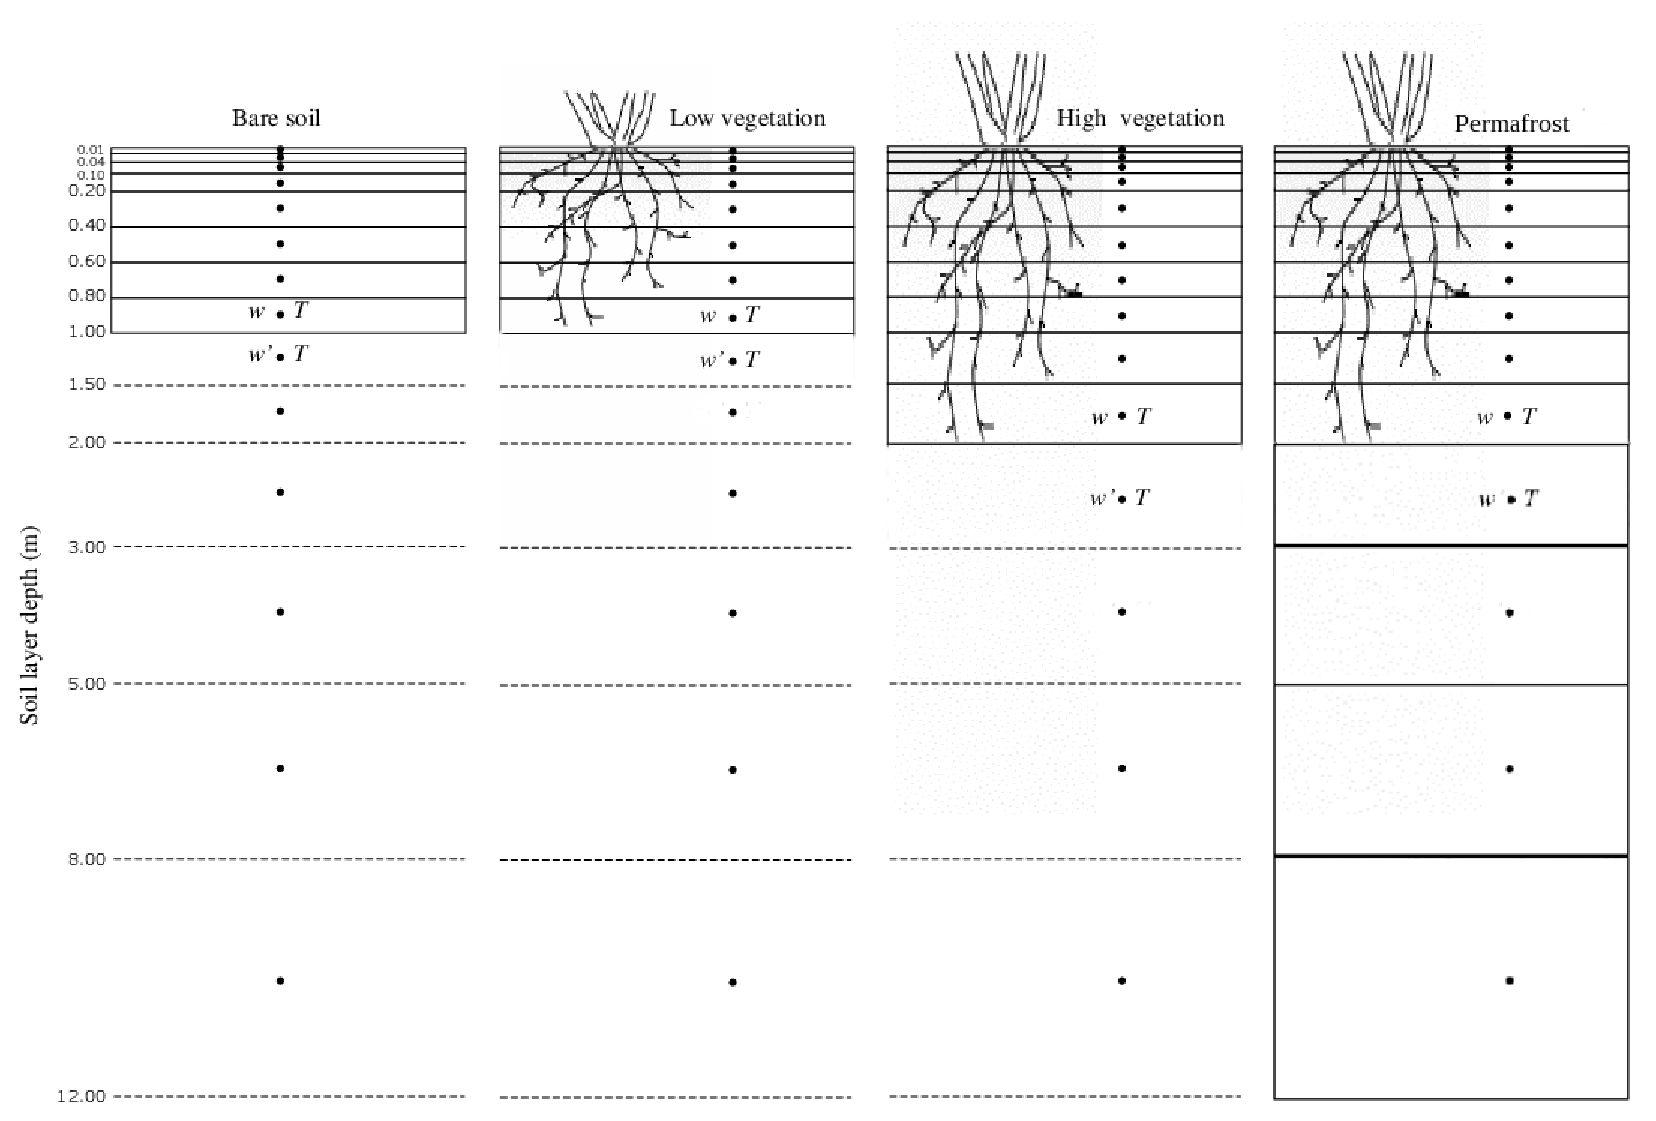
\includegraphics[angle=0, width=15cm]{EPS/isba-dif_water-thermal-grids.eps}}
\caption{
The ISBA-DF soil grid configurations. Prognostic variable nodes (for
liquid water, $w_g$, soil ice, $w_{gf}$ and temperature, $T_g$) are located
at the center of each of the layers. There are 14 layers used for
thermal computations, and the same default 
grid thicknesses are used everywhere (note this can be modified by the
user). Hydrological grids are enclosed
by the solid black lines: thus the soil water prognostic equations do
not extend as deeply as the thermal computations except for areas/grid
cells with permafrost. See Decharme \etal (2013) for more details.
}
\label{fig:isba-dif_soil_grid}
\end{figure}
%%%%%%%%%%%%%%%%%%%%%%%%%%%%%%%%%%%%%%

Finally, the thicknesses of the current 14 layers have
been arranged to minimize numerical errors in solving
energy and water diffusion equations, especially in the first
meter of soil (Decharme \etal 2011). Note that the thermal
and/or hydrological lower boundary conditions of the soil,
as well as the thickness and the number of layers, can be
modulated by the user.

\paragraph{Numerical solution of the soil temperature equation}
%
Neglecting the phase transformation term,
Eq.~(\ref{teq}) can be written using an implicit time scheme as
%
\begin{equation}\label{teqcn}
{T_j}^{n}\,\,=\,\, {T_j}^{n-1} \,+\, 
\frac{\Delta t }{c_{g\,j}\,\Delta z_j}
\left[
\left(1-\varphi\right)
\left( {G_{j-1}}^{n-1} \,-\, {G_j}^{n-1} \right) +
\varphi
\left( {G_{j-1}}^{n} \,-\, {G_j}^{n} \right)
\right] 
\end{equation}
%
where $\varphi=1$ (backward difference) is currently used
for the soil temperature profile ($\varphi=1/2$ corresponds
to the Crank-Nicolson scheme).
Using either scheme,
the linear set of diffusion equations can be cast in tridiagonal
form and solved with relative ease. Although the Crank-Nicolson
scheme is more accurate (second order), the surface energy budget
equation is solved in ISBA using the backward difference scheme,
so for consistency this scheme is used to evaluate the diffusion term
in Eq.~(\ref{teq}).

The superscripts $n-1$ and $n$ represent the values
at the beginning and end of the time step, $\Delta t$, respectively.
The solution method is shown in Appendix B.
Once the new temperature profile has been determined, phase changes
are evaluated and the profile is updated. The phase change method
is described in section 4.

%=========================================================================================================
\subsubsection{Liquid Soil Water}
%=========================================================================================================
%
The vertical soil water flux from Eq.~(\ref{cont1}) is 
derived assuming soil water transfer arises due to
pressure gradients and a background drainage, and it is
expressed as
%
%%%%%%%%%%%%%%%%%%%%%%%%%%%%%%%%%%%%%%%%%
\beq\label{darcy}
F \,\,=\,\, -k\, \frac{\partial}{ \partial z} 
\left( \psi \,+\, z \right) 
\,-\, \frac{D_{\nu\psi}}{\rho_w}\frac{\partial \psi}{\partial z}
\eeq
%%%%%%%%%%%%%%%%%%%%%%%%%%%%%%%%%%%%%%%%%
%
where $F$ is the vertical soil water flux (${\rm m\,s^{-1}}$),
$k$ is the hydraulic conductivity (${\rm m\,s^{-1}}$),
$\psi$ is the soil matric potential (m),
%, $K_d$ 
%is an additonal linear background (low) drainage term (m s${-1}$),
and $z$ is the soil depth (m). 
The first term on the right hand side
of Eq.~\ref{darcy} represents Darcy's law for liquid
water transfer. The second term 
represents the water flux due to vapor transfer.
%The third is used to maintain a minimum 
%streamflow under dry conditions.
The isothermal vapor conductivity $D_{\nu\psi}$ 
(kg m$^{-2}$ s$^{-1}$) is a function of soil texture,
water content and temperature following Braud \etal (1993)\nocite{Braud1993-10-01},
except for some slight modifications due to the inclusion of
soil ice outlined here.

This representation of the fluxes results in the so-called
``mixed-form'' of the Richard's equation. It permits the
use of a heterogenous soil texture profile (by considering
the gradient of matric potential which is continuous as opposed to soil
water content which is not necessarily continuous when the soil
properties vary).

Finally, when soil ice is present, Eq.~\ref{darcy} is modified
as
%
%%%%%%%%%%%%%%%%%%%%%%%%%%%%%%%%%%%%%%%%%
\beq\label{darcy_frz}
F \,\,=\,\, -k\, \left(
\wp \, \frac{\partial\psi}{ \partial z} 
\,-\, z \right) 
\,-\, \frac{\wp\,D_{\nu\psi}}{\rho_w}\frac{\partial \psi}{\partial z}
\eeq
%%%%%%%%%%%%%%%%%%%%%%%%%%%%%%%%%%%%%%%%%
%
where the non-dimensional coefficient $\wp$ has been introduced 
which acts to limit
vertical diffusion in the presence of a freezing front
(see Eq.~\ref{iceimp}).

\paragraph{Flux parameterization}
%
The vertical soil water flux term [Eq.~(\ref{darcy})] 
can be expressed in more compact form as:
%
\begin{equation}\label{darcy2}
F \,\,=\,\, -\eta \, \frac{\partial \psi}{\partial z} \,-\, k
%- \zeta
\end{equation}
%
where $\eta$ (${\rm m^2\,s^{-1}}$)
represents the effective diffusion coefficient.
% and $\zeta$
%is the total drainage flux (m s$^{-1}$).
It is expressed as
%
%%%%%%%%%%%%%%%%%%%%%%%%%%%%%%%%%%%%%ù
\begin{equation}
\eta = \wp \, \left(k \,+\, \frac{D_{\nu\psi}}{\rho_w}\right) 
%\zeta &= k + K_d \cr
\end{equation}
%%%%%%%%%%%%%%%%%%%%%%%%%%%%%%%%%%%%%ù
%
The first term on the RHS of
Eq.~\ref{darcy2} is the diffusion term and usually
is positive (directed upward), the exceptions possibly being
during precipitation, snowmelt or perhaps soil thaw events.
The second term on the RHS of Eq.~(\ref{darcy2}) 
represents total drainage and is always directed (positive) downward.
During strong infiltration events (rainfall, snowmelt etc...)
generally $k$ dominates the (downward) water flux.
%
Note that if vapor diffusion is neglected and the soil is not frozen,
%and the linear drainage term (option) is negligible, 
the vertical flux
given by Eq.~(\ref{darcy})
collapses into the standard Darcy flux expression
for liquid water movement:
%
%%%%%%%%%%%%%%%%%%%%%%%%%%%%%%%%%%%%%%%%%%%%%%%%%%%%%%%%
\begin{equation}
\label{darcy3}
F \,\,=\,\, -k\, \frac{\partial }{\partial z} 
\left( \psi \,+\, z \right) 
\end{equation}
%%%%%%%%%%%%%%%%%%%%%%%%%%%%%%%%%%%%%%%%%%%%%%%%%%%%%%%%
%
%AABHERE

\subparagraph{Soil Freezing}
%
As a soil freezes, ice is assumed to become part
of the soil matrix thereby reducing the liquid water 
holding capacity of the soil. The degree of saturation
of the soil by liquid water is expressed 
%following Kowalczyk (1998) 
as
%
%
%%%%%%%%%%%%%%%%%%%%%%%%%%%%%%%%%%%%%%%%%%%%%%%%%%%%%%%%
\begin{equation}
\label{srl}
\Theta \,\,=\,\, \frac{w-w_i}{w_{sat}-w_i}
\,\,=\,\, \frac{w_l}{w_{sat\,l}}
\hskip.5in (0\,\leq\, \Theta \,\leq\, 1)
\end{equation}
%%%%%%%%%%%%%%%%%%%%%%%%%%%%%%%%%%%%%%%%%%%%%%%%%%%%%%%%
%
%
where $w_{sat\,l}$ represents the soil liquid water
holding capacity. The porosity is decreased in the presence of
soil ice as it is assumed ice becomes part of the soil matrix
(see Boone \etal (2000) for more information).

The hydraulic conductivity and soil water potential
are related to the liquid volumetric soil water content
through the relations (Clapp and Hornberger, 1978):
%
\beq\label{k}
 k \,\,=\,\,k_{sat}\,{\Theta}^{2b+3} 
\eeq
%
\beq\label{psi}
 \psi =\,\,\psi_{sat}\,{\Theta}^{-b} 
\eeq
%
where $b$ is an empirical parameter, $k_{sat}$ is the 
hydraulic conductivity at saturation, $\psi_{sat}$ is
the water potential at saturation and $w_{sat}$ is the soil
porosity. 
In recent years, several SVATs (eg. VISA: Yang and Niu, 2003\nocite{Yang2003})
have adopted the idea
that the saturated hydraulic conductivity decreases
exponentially with increasing soil depth (Beven and Kirby, 1979). 
This can be handled by ISBA-DF since Richard's equation
is expressed in mixed-form (i.e. a heterogeneous profile
of $k_{sat}$ can be specified).

Soil ice has the effect of decreasing the hydraulic
conductivity relative to a thawed soil
with the same total soil moisture.
The ice impedance coefficient is represented by
$\wp$. It is calculated following Johnsson and Lundin (1991):
%
\begin{equation}\label{iceimp}
\wp \,\,=\,\,{10}^{-a_\wp \,w_i/w}
\end{equation}
%
where the coefficient $a_\wp$ is currently assigned a value
of 6 proposed by Lundin (1990)\nocite{Lundin1990}. This coefficient prevents
an overestimation of the upward 
liquid water flux to the freezing front. Note that the model
is rather sensitive to this parameter, and a calibration might
be required to obtain optimal agreement with observations.
The dependence of $\wp$ on ice content ratio ($w_i/w$)
is shown in Fig.~\ref{iceimped}. 
Note that the effect of this 
coefficient is currently under investigation, and that alternate
formulations (such as dependence on soil temperature rather than
soil ice) will also be explored.

\begin{figure}[h]
		 \begin{center}
		 \psfig{figure=EPS/Eice.eps,width=8cm}
		 \caption{The dependence on the water flux impedance factor ($\wp$)
on soil ice fraction ($w_i/w$) for various
values of $a_\wp$ (denoted as ``Eice'' in the figure). 
This coefficient is multiplied by the
vertical soil water flux, and as such can strongly modulate
vertical flow of liquid water and subsequent
freezing.}
		 \label{iceimped}
		 \end{center}
\end{figure}



\subparagraph{Vapor diffusion}
%
The isothermal vapor conductivity can be expressed as
%
\begin{equation}\label{vapdif}
D_{\nu\psi} \,\,=\,\,
D_\nu \, \frac{\partial\rho_\nu}{\partial\psi}
\end{equation}
%
where $\rho_\nu$ represents the water vapor density in the air-filled pore 
space of the soil, and $D_\nu$ represents an effective molecular
diffusivity (Milly (1982)\nocite{Milly1982}). It can be written following
Braud \etal (1993) as
%
\begin{equation}\label{vapmoldif}
D_\nu \,\,=\,\,
D_{\nu a} \,\alpha_\nu \, f_{\nu a}
\frac{p}{ \left(p-p_\nu\right)}
\end{equation}
%
where the tortuosity is $\alpha_\nu = 0.66$,
and the atmospheric and soil vapor pressures
are represented by $p$ and $p_\nu$, respectively.
The function $f_{\nu a}$ is defined as
%
%%%%%%%%%%%%%%%%%%%%%%%%%%%%%%
\[ f_{\nu a} = \left\{ \begin{array}{ll}
\left[w_{sat} - \left(w_l+w_i \right)\right]
\left[1 \,+\, 
{\left(w_l+w_i \right)/
\left(w_{sat}-w_k \right)}
\right]
& \mbox{if $\left(w > w_k\right)$} \\
%
w_{sat} & \mbox{if $\left(w \leq w_k \right)$}
\end{array} 
\right. \] 
%%%%%%%%%%%%%%%%%%%%%%%%%%%%%%
%
where $w_k$ is a parameter which defines the point corresponding to
the loss of continuity of the liquid phase in the soil pores 
(0.05 m$^3$ m$^{-3}$ for the current study). The function
$f_{\nu a}$ is related to the available pore space for vapor, or volumetric 
air content ($w_{sat}-w_l-w_i$).
The molecular diffusivity coefficient for water
vapor is given as
%
%
%%%%%%%%%%%%%%%%%%%%%%%%%%%%%%%%%%%%%%%%%%%%%%%%%%%%%%%%
\begin{equation}
\label{moldify}
D_{\nu a} \,\,=\,\,
c_\nu \, \left(\frac{p_0}{ p}\right)
{\left(\frac{T }{ T_f}\right)}^{n_\nu}
\end{equation}
%%%%%%%%%%%%%%%%%%%%%%%%%%%%%%%%%%%%%%%%%%%%%%%%%%%%%%%%
%
%
where $c_\nu = 2.17 \times {10}^{-5}$ m$^2$ s$^{-1}$,
$n_\nu = 1.88$, and $p_0 = {10}^6$ Pa. It is assumed that the soil
water vapor is in equilibrium with the liquid, and that
the air is saturated with respect to the 
ice present in the soil
so that the vapor density can be expressed as
%
%
%%%%%%%%%%%%%%%%%%%%%%%%%%%%%%%%%%%%%%%%%%%%%%%%%%%%%%%%
\begin{equation}
\label{vapden}
\rho_\nu \,\,=\,\,
\rho_{\nu\,sat}(T)
\chi_{sat} \, h_\nu
\,+\,
\left( 1-\chi_{sat}\right) \rho_{\nu\,sat\,i}{\rm min}(T,T_f)
\end{equation}
%%%%%%%%%%%%%%%%%%%%%%%%%%%%%%%%%%%%%%%%%%%%%%%%%%%%%%%%
%
%
where the humidity is given by
%
%
%%%%%%%%%%%%%%%%%%%%%%%%%%%%%%%%%%%%%%%%%%%%%%%%%%%%%%%%
\begin{equation}
\label{vaphum}
h_\nu \,\,=\,\,
{\rm exp}\left( \frac{\psi\,g}{ R_\nu \,T}\right)
\end{equation}
%%%%%%%%%%%%%%%%%%%%%%%%%%%%%%%%%%%%%%%%%%%%%%%%%%%%%%%%
%
%
The soil ice factor is defined as
%
%%%%%%%%%%%%%%%%%%%%%%%%%%%%%%%%%%%%%%%%%%%%%%%%%%%%%%%%
\begin{equation}
\label{chisat}
\chi_{sat} = \left(w_{sat}-w_i\right)/w_{sat}
\end{equation}
%%%%%%%%%%%%%%%%%%%%%%%%%%%%%%%%%%%%%%%%%%%%%%%%%%%%%%%%
%
% 
Taking the derivative of $\rho_\nu$ with respect to $\psi$
and substituting the resulting expression and
Eq.~(\ref{vapmoldif}) into Eq.~(\ref{vapdif}) 
using the ideal gas law for water
vapor results in
%
%
%%%%%%%%%%%%%%%%%%%%%%%%%%%%%%%%%%%%%%%%%%%%%%%%%%%%%%%%
\begin{equation}
\label{vapdif2}
D_{\nu\psi} \,\,=\,\,
\frac{\alpha_\nu \,p }{ \left( p-p_\nu\right)}
\frac{D_{\nu a}\,f_{\nu a}\,\chi_{sat} \,g \, p_{\nu\,sat} \,h_\nu
}{ {\left(R_\nu \,T\right)}^2}
\end{equation}
%%%%%%%%%%%%%%%%%%%%%%%%%%%%%%%%%%%%%%%%%%%%%%%%%%%%%%%%
%

\begin{figure}[h]
		 \begin{center}
		 \psfig{figure=EPS/vapdif.eps,width=8cm}
		 \caption{Soil vapor diffusion coefficient ($d_\nu$) for four soil
textures assuming constant soil temperature
and pressure.}
		 \label{vapdiffig}
		 \end{center}
\end{figure}

The diffusion coefficient ($d_\nu$) is
shown in Fig.~(\ref{vapdiffig}) 
for four soil textures 
over the entire range of soil wetness
($w_l/w_{sat}$) assuming a constant
temperature and pressure of 300 K and 101325 Pa,
respectively. It is largest, in general, for the
most coarse textured soils approximately
at or below the soil permanent wilting point value.
A comparison between the vapor diffusion and
the hydraulic conductivity are shown in
Fig.~(\ref{vapdiffig2}). This shows that vapor diffusion
comprises the most significant contribution to 
the net diffusion process over a soil water range
around the wilting point. In the ISBA force-restore method, this vapor
phase transfer is parameterized within the coefficient $C_1$ for dry soil
(Braud \etal (1993) and Giordani (1996)\nocite{Giordani1996}).
%
As a final note, strictly speaking, vapor diffusion involves latent
heating effects which couples the mass and heat eqiuations very
tightly over a certain range of temperature and soil moisture. 
But currently in ISBA, the effect of vapor diffusion is simply modeled
by increasing the effective diffusivity of liquid transfer as a first
order approach (thus, mass is conserved and energy is unchanged) since
historically, the goal was to maintain baresoil evaporation under dry
but sufficiently hot surface conditions. Future work could consist in adding
the latent heating effect.

\begin{figure}[h]
		 \begin{center}
		 \psfig{figure=EPS/vapdif2.eps,width=8cm}
		 \caption{The total hydraulic conductivity contributions
from liquid water ($k$) and vapor ($D_{\nu\psi}$)
for three soil textures as a function of soil wetness.
The soil temperature and surface atmospheric pressure have constant
values of 285 K and 10$^5$ Pa, respectively.}
		 \label{vapdiffig2}
		 \end{center}
\end{figure}

%\subparagraph{Linear Drainage}
%
%ISBA is increasingly used in studies for which river hydrology is simulated.
%The standard Richard's equation poses a problem for dry conditions in
%that the observed constant minimum riverflow occuring during dry seasons
%is poorly simulated. The actual cause of such flows is most likely subterranian
%lakes, surface lakes, water table interactions, etc., which are all not currently 
%explicitly modeled by ISBA. The most simplistic fix to this problem is to
%impose a linear drainage term which can be calibrated based on observed minimum
%riverflows outside of periods of active precipitation or snowmelt.
%
%Etchevers \etal (2002)\nocite{Etchevers2002} calibrated such a parameter for the 3-layer ISBA
%Force-Restore approach and greatly improved discharge statistics for certain
%sub-basins within the Rhone basin in France. In this method, a drainage
%is calculated assuming the water content is at some small increment just
%above field capacity (thereby resulting in a steady, but relatively small
%drainage flux). Adapting this method into the current model results in
%
%%%%%%%%%%%%%%%%%%%%%%%%%%%%%%%%%%%%%%%%%%%%%%%%%%%%%%%%
%\begin{equation}
%K_d = k_{sat} {\left[\left(w_{fc} + w_{drain}\right)/w_{sat}\right]}^{2b+3} \times
%\Biggr\lbrace \frac{
%\left[{\rm min}\left(w_{fc},w_l\right)-w_{min}\right] 
%}{\left(w_{fc}-w_{min}\right)
%}\Biggr\rbrace
%\end{equation}
%%%%%%%%%%%%%%%%%%%%%%%%%%%%%%%%%%%%%%%%%%%%%%%%%%%%%%%%
%
%
%The term on the left of the multipication sign
%is constant in time.
%The rightmost term is a linear scaling term which reduces the constant
%drainage as the source soil layer dries out. The field capacity water
%content is given by $w_{fc}$. The $w_{drain}$ can be calibrated and is generally
%on the order of 0.001 m$^3$ m$^{-3}$, although it can vary by an order
%of magnitude. It is zero (therefore $K_d=0$) when this option is off
%(i.e. local scale studies etc.).

\paragraph{Layer averaging}
%
Integrating Eq.~(\ref{cont1})
downward into the soil to obtain the prognostic equation for
the layer-average volumetric liquid water content for each $j$ layer
gives
%
\beq\label{int_continuity}
\int_{-z_j}^{-z_{j-1}} 
\frac{\partial w_l}{ \partial t } dz \,\,=\,\,
-\int_{-z_j}^{-z_{j-1}} 
\frac{\partial F}{ \partial z} dz \,-\,
\int_{-z_j}^{-z_{j-1}} \left(S_l-\frac{\Phi}{ L_f\rho_w}\right) dz
\eeq
%
where
%
\beq\label{avgtheta}
w_{l\,j} \,\,=\,\, \frac{1}{ \Delta z_j} \int_{-z_j}^{-z_{j-1}}
w_l dz
\eeq
%
$w_{l\,j}$ is the layer averaged volumetric liquid water
content ($j=1,...,N$).

Carrying out the integration in Eq.~\ref{int_continuity} using 
Eq.~\ref{avgtheta} yields
%
%%%%%%%%%%%%%%%%%%%%%%%%%%%%%%%%%%%%%%%%%%%%%%%%%%%%%%%%
\begin{equation}
\label{avgcont}
\Delta z_j {\frac{w_{l\,j}}{\partial t}} \,\,=\,\,
F\Big\vert_{-z_j} \,-\, 
F\Big\vert_{-z_{j-1}} \,-\, Q_j \,-\,
{\frac{\Delta z_j\, \Phi_j}{L_f\rho_w}} 
\end{equation}
%%%%%%%%%%%%%%%%%%%%%%%%%%%%%%%%%%%%%%%%%%%%%%%%%%%%%%%%
%
%
where 
%
\beq\label{avgsinkQ}
Q_j \,\,=\,\, \Delta z_j\,S_j 
\eeq
%
is in kg m$^{-2}$ s${-1}$.
The flux across a model level ($z_j$) is written as
%
%%%%%%%%%%%%%%%%%%%%%%%%%%%%%%%%%%%%%%%%%%%%%%%
\begin{subequations}
\begin{align}
\label{waterflux}
F\Big\vert_{-z_j} \,\,=&\,\,
F_j \,\,=\,\,
{\overline\eta}_j \,
\left[ \frac{\psi_{j+1}-\psi_{j}}
{\left(\Delta z_j+\Delta z_{j+1} \right)/2}\right] 
\,-\,{\overline k}_j 
\\
\label{waterflux_b}
{\overline\eta}_j \,\,=&\,\, \wp_j \left( {\overline k}_j + 
\frac{{\overline D}_{\nu\psi,j}}{\rho_w} \right)
\end{align}
\end{subequations}
%%%%%%%%%%%%%%%%%%%%%%%%%%%%%%%%%%%%%%%%%%%%%%%
%
where ${\overline k}_j$ and ${\overline D}_{\nu\psi,j}$ 
(both in m s$^{-1}$) represent the geometric means over two
consecutive
nodes of the soil hydraulic conductivity
and isothermal vapor conductivity values, respectively.
The inter-facial hydraulic conductivity is defined as
%
%%%%%%%%%%%%%%%%%%%%%%%%%%%%%%%%%%%%%%%%%%%%%%%
\begin{equation}
\label{kinterp}
{\overline k}_j = \sqrt{k_j\left(\psi_j\right) 
\times k_{j+1}\left(\psi_{j+1}\right)}
\end{equation}
%%%%%%%%%%%%%%%%%%%%%%%%%%%%%%%%%%%%%%%%%%%%%%%
%
The choice of an appropriate intra-block approximation for unsaturated
hydraulic conductivity has been pointed out as critical in the
numerical solution of unsaturated flow by many studies.
As discussed in Decharme et al. (2011)/nocite{Decharme2011},
%(Haverkamp et al., 1977; 
%Haverkamp and Vauclin, 1979; 
%Hornung and Messing, 1983;
%Schnabel and Richie, 1984; 
%Warrick, 1991; 
%Zaidel and Russo, 1992; 
%Feng et al., 2007). 
many studies have demonstrated 
that the geometric mean generates little weighting error, improves the
simulated infiltration front, and is generally applicable in all
situations.

%AABHERE
 

% OLD ---------------------------------------------------------
% OLD psi interp
%
%${\tilde\psi}$ represents the so-called interfacial matric
%potential. It is calculated from
%%
%\beq\label{sinterp}
%{\tilde\psi}_{j} \,\,=\,\,
%\delta_{\psi\,j} \, \psi_{j} \,+\, (1-\delta_{\psi\,j})
%\psi_{leq\,j} 
%\eeq
%
%where the delta function $\delta_{\psi\,j}$ is
%defined as
%
%
%%%%%%%%%%%%%%%%%%%%%%%%%%%%%%
%\[ \delta_{\psi\,j} = \left\{ \begin{array}{ll}
%        1 & \mbox{if $\psi_{j} \geq \psi_{leq\,j}$}
%\\
%        0 & \mbox{if $\psi_{j} < \psi_{leq\,j}$}
%\end{array} 
%\right. \] 
%%%%%%%%%%%%%%%%%%%%%%%%%%%%%%
%
%hydrostatic equilibrium.
%It is calculated assuming that the total matric potential
%or head is constant from the layer interface ($z_j$)
%to the mid-point of the layer below
%(Noilhan and Planton (1989), Koster and 
%Suarez (1996)\nocite{Koster1996}): ${\partial\psi/\partial z}=-1$:
%
%%%%%%%%%%%%%%%%%%%%%%%%%%%%%%%%%%%%%%%%%%%%%%%%%%%%%%%%
%\begin{equation}
%\label{psieq}
%\psi_{leq\,j} \,\,=\,\, \psi_{j+1} \,-\,
%\left(\Delta z_j+\Delta z_{j+1}\right)/4 \,\,\,.
%\end{equation}
%%%%%%%%%%%%%%%%%%%%%%%%%%%%%%%%%%%%%%%%%%%%%%%%%%%%%%%%
%
%
%From Eq.~(\ref{sinterp}), diffusivity and conductivity
%are evaluated using the so-called upstream value of the matric potential,
%which is similar to the simple model proposed by Mahrt and 
%Pan (1984)\nocite{Mahrt1984},
%except that the equilibrium matric potential value is used in
%place of the lower layer matric potential (equivalently the
%volumetric water content in their case as they assumed a
%homogenous soil texture profile). As in Mahrt and Pan (1984),
%the upper layer matric potential (water content in their case)
%is used in the presence of a wetting front. Such an interpolation
%is needed due to the coarse nature of the vertical grid mesh typically
%used in SVATs intended for atmospheric models.
%
% OLD psi interp
% OLD ---------------------------------------------------------

A graphic representation of the interpolation method is
shown for two contiguous soil layers with different
textures (and therefore, different soil hydraulic 
properties) in Fig.~\ref{kint}. 

\begin{figure}[h]
		 \begin{center}
		 \psfig{figure=EPS/kint_anglais.eps,width=10cm}
		 \caption{The interfacial hydraulic
                   conductivity. ${\overline k}_j$
represents the hydraulic conductivity centered at $z_j$, and
${\tilde\Delta} z_j = 
\left(\Delta z_{j} + \Delta z_{j+1}\right)/2$.}
		 \label{kint}
		 \end{center}
\end{figure}

%This method results in
%a better approximation of the soil water flux than 
%specifying that the flux from the mid-point of 
%layer $\Delta z_j$ to $z_j$ is equal to that from
%layer $z_j$ to the mid-point of layer $\Delta z_{j+1}$
%(as is used to derive the soil heat flux),
%as the diffusivity and conductivity are more consistent
%with the soil water gradient (Mahrt and Pan (1984)). 

\paragraph{Boundary Conditions}
%
\subparagraph{Lower Boundary}
%
The lower boundary condition is modeled as gravitational drainage
(vertical diffusion is neglected). The mean water content of the lowest
layer is used to evaluate the flux
so that from Eq.~(\ref{waterflux}) one can write
%
%%%%%%%%%%%%%%%%%%%%%%%%%%%%%%%%%%%%%%%%%%%%%%%%%%%%%%%%
\begin{equation}
\label{lowerwaterbc}
F_N \,\,=\,\, -k_N 
%F_N \,\,=\,\, -\zeta_N \,\,=\,\, -k_N 
%- K_d 
\end{equation}
%%%%%%%%%%%%%%%%%%%%%%%%%%%%%%%%%%%%%%%%%%%%%%%%%%%%%%%%
%
%
%Under moist conditions, $F_N \approx -k_N$,
%whereas for very dry conditions, it is possible
%that $K_d$ dominates the drainage (depending on the
%value specified for $K_d$).
%
The diffusion term
(i.e. capillary rise across the lower model boundary) 
can be significant, however, when the water table is near
$z_N$. An option exists for utilizing this information
using a simple expression consistent with the vertical flux
formulation used for the other model layers.
%, however
%it is currently not included in the current model
%release (as typically water table information is
%not available in atmospheric models).
%
In this case, $F_N$ is modified to be
%
%%%%%%%%%%%%%%%%%%%%%%%%%%%%%%%%%%%%%%%%%%%%%%%%%%%%%%%%
\begin{align}
\label{lowerwaterbcx}
F_N \,\,=&\,\, -k_N \left[
f_{wtd}
\left( \frac{\psi_{N}-\psi_{sat}}{\Delta z_{wtd}} + 1\right)
\,+\, \left(1- f_{wtd}\right)
\right]
\\
\label{lowerwaterbcxz}
\Delta z_{wtd} \,\,=&\,\,
{\rm min}\left( z_N,\,z_{wtd}\right) \,-\,
\left( z_N + z_{N-1}\right)/2
\end{align}
%%%%%%%%%%%%%%%%%%%%%%%%%%%%%%%%%%%%%%%%%%%%%%%%%%%%%%%%
%
where $f_{wtd}$ is the gird-cell fraction 
where capillary rise occurs. It
can be 1 at the local scale or depend on topography at larger
scales. Indeed, only a fraction of the grid cell corresponding to the
flat valleys and alluvial plains should be affected by water
capillary rises. This fraction must reflect the subgrid topographical
heterogeneity inside each grid cell, which can be significant, for
example, 
when considering the coarse resolution of the climate models. A
grid cell with steeper topography would be affected by upward
capillary fluxes over a small fraction of the grid cell, 
unlike those characterized by relatively 
flatter terrain. See 
Vergnes et al. (2014)\nocite{Vergnes2014} for more details.


\subparagraph{Upper Boundary}
%
The upper boundary condition represents infiltration.
%
By default, the soil infiltration $I$ is equal to the
potential (supply limited) infiltration rate, i.e. $I = R_t$. 
%where $R_t$
%(m s$^{−1}$) is the through-fall rate (sum of canopy drip, precipitation
%and snow-melt). 
This case is specially relevant for local scale
studies. 
The soil-water infiltration is put preferentially in the first layer. If
this first layer can not contain this amount of water, the remaining
is forced into the next layer and so forth (downward).

An Horton runoff option exists that computes the soil infiltration via
a Green and Ampt (1911) approach (Decharme et al. 2013)\nocite{decharme_ea_2013}. 
This approach, based on Darcy’s law, includes the hydrodynamic parameters
of the soil and determines the infiltration capacity of soil over the
time. It represents the soil infiltration as a wetting front in which
the hydraulic gradient is uniform. In ISBA-DF, the analytical form of the
Green-Ampt approach is used to determine the maximum amount of water
that infiltrates the soil to a depth close to 0.1 m (the thickness
generally used for relatively large time steps). 
The infiltration capacity, $I_c$
(kg m$^{-2}$ s$^{-1}$), is therefore parameterized as:
%
%%%%%%%%%%%%%%%%%%%%%%%%%%%%%%%%%%%%%%%%
\begin{equation}
\label{eq:infiltration_capacity}
%
I_c = \frac{\rho_w}{z_{nic}} \sum_{i=1}^{nic}
\left[
\wp_i \, k_{sat,i}
\left(
\frac{\psi_{sat}-\psi_{i}}{\Delta z_i} \,+\, 1
\right) \Delta z_i
\right]
\end{equation}
%%%%%%%%%%%%%%%%%%%%%%%%%%%%%%%%%%%%%%%%
%
where $z_{nic}$ (m) 
represents the depth of the layer $nic$ that is the nearest 0.1 m, and 
$\Delta z_i$ (m) is the thickness of each of the $i$ layers. 
Finally, the soil-water
infiltration in ISBA-DF can be computed by comparing this infiltration
capacity with the flux of water reaching the soil:
%
%%%%%%%%%%%%%%%%%%%%%%%%%%%%%%%%%%%%%%%%
\begin{equation}
\label{eq:upperwaterbc_nosubgrid}
%
I = {\rm min}\left(R_t, \, I_c \right)
\end{equation}
%%%%%%%%%%%%%%%%%%%%%%%%%%%%%%%%%%%%%%%%
%
All of the excess water (i.e. defined as $R_t-I$ when it is $>0$) 
is treated as a “Horton” surface runoff flux
whereas the soil infiltration is treated as a moisture source term.

For non-local scale applications, an alternate form of 
generating surface
runoff is needed. 
In this case, infiltration is computed as:
%
\beq\label{upperwaterbc}
I \,\,=\,\,{\rm min}(R_t-Q_r,\,I_c)
\eeq
%
It can also be computed via a variable infiltration capacity 
(VIC: Dumenil and Todoni, 1992)\nocite{Dumenil1992}
sub-grid surface runoff scheme
used in ISBA (Habets \etal 1999)\nocite{Habets1999}.
%
In this scheme,
$Q_r$ represents sub-grid surface runoff from saturated regions
within the computational unit/cell
(See Eq.s~\ref{eq:i_m_vic_model}-\ref{eq:a_vic_model} for the
theoretical background).
It is computed using a similar form as that for the Force-Restore
approach (Eq.s~\ref{qrc}-\ref{qrz}):
%
%%%%%%%%%%%%%%%%%%%%%%%%%%%%%%%%%%%%%%%%%%%%%%%%%%%%
\begin{subequations}
\begin{align}
\label{eq:qrc_df}
Q_{r\,{\rm crit}} \,\,=\,\, &
{\left[1 - {\left({\overline w}_r-{\overline w}_{c,min}\right)\over 
\left({\overline w}_{sat}-{\overline w}_{c,min}\right)}\right]}^{1/(1+{\rm b})}
\,-\,
{R_t \Delta t \over \rho_w z_r}
\left[{ 1\over
(1+{\rm b})\left({\overline w}_{sat}-{\overline w}_{c,min}\right)
}\right]
\\
\label{eq:qr_df}
Q_r \,\,=\,\, & R_t - {\rho_w z_r \over\Delta t}
\Biggr\lbrace
\left({\overline w}_{sat}-{\overline w}_r\right)-
\left({\overline w}_{sat}-{\overline w}_{c,min}\right) 
{\left[{\rm max}\left(0,\,Q_{r\,{\rm crit}}\right)\right]}^{1+{\rm b}}
\Biggr\rbrace
\end{align}
\end{subequations}
%%%%%%%%%%%%%%%%%%%%%%%%%%%%%%%%%%%%%%%%%%%%%%%%%%%%
%
with the constraints (as in Eq.~\ref{qrz}, but using a layer averaged
$w_{c,min}$):
%
%%%%%%%%%%%%%%%%%%%%%%%%%%%%%%%%%%%%%%%%%%%%%%%%%%%%%%%%
\begin{equation}
\label{eq:qrz_df}
Q_r \,\,=\,\, 0
\hskip.5in
{\rm if}\hskip.2in
\left(Q_r < 0 \right) 
\hskip.2in {\rm or}\hskip.2in 
\left({\overline w}_r \leq {\overline w}_{c,min}\right) 
\end{equation}
%%%%%%%%%%%%%%%%%%%%%%%%%%%%%%%%%%%%%%%%%%%%%%%%%%%%%%%%
%
%where $R_t$
%(m s$^{−1}$) is the through-fall rate (sum of canopy drip, precipitation
%and snow-melt). 
%${\overline w}_r$ represents the average total water
%
Note that currently, $w_{c,min}=w_{wilt}$ by default until further
studies can be done.
$Q_r$ is evaluated using the average total soil moisture, ${\overline w}_r$,
integrated from the surface down
to a characteristic depth, $z_r$. It is defined as
%
%%%%%%%%%%%%%%%%%%%%%%%%%%%%%%%%%%%%%%%%%%%%%%%%%%%%%%%%
\begin{equation}
\label{eq:water_content_avg_dif_vic}
{\overline w}_r = 
{\frac
{\left(\sum_{j=1}^{N_r} \Delta z_j \, w_j \right) + 
w_{N_r+1}{\rm max}\left(0,\,z_r-z_{N_r}\right)} 
{\left(\sum_{j=1}^{N_r} \Delta z_j \right) + 
{\rm max}\left( 0,\,z_r-z_{N_r}\right)}
}
\hskip.5in
\left(z_r \leq z_N\right)
\end{equation}
%%%%%%%%%%%%%%%%%%%%%%%%%%%%%%%%%%%%%%%%%%%%%%%%%%%%%%%%
%
where $N_r$ is the total number of soil layers for which
$z_r \geq z_j$ (i.e. the depth is greater than or equal to
the lower boundary of the
soil layer $j$). Note that the porosity and wilting point volumetric water
contents are also averaged over $z_r$ using the same operator.
This depth should be at least several tens of centimeters 
thick (Liang \etal 1996).

It should also be noted that several authors use a form
of Darcy's law assuming the soil right at the surface
is saturated as the maximum potential infiltration rate
(Mahrt and Pan, 1984\nocite{Mahrt1984}; 
Abramopoulos \etal 1988\nocite{Abramopoulos1988}).
This, however, has a very minimal impact on the infiltration
(compared to the above equations) for the time and space scales
considered in typical ISBA applications, and the linearization
of such a term can pose some numerical problems (the linearized
surface flux can actually exceed the amount of water available
for infiltration under some rare circumstances). 
%For these two
%reasons, Eq.~(\ref{infilt}) is used currently in ISBA.

\paragraph{Solution method}
%
The equation for liquid water transfer is
solved using:
%
%%%%%%%%%%%%%%%%%%%%%%%%%%%%%%%%%%%%%%%%%%%%%%%%%%%%%%%%
\begin{equation}
\label{watercn}
\varrho_j
({w_{l\,j}}^{n}-{w_{l\,j}}^{n-1}) \,\,=\,\,
\left(1-\varphi\right)
\left({F_j}^{n-1} \,-\,{F_{j-1}}^{n-1} \right)
\,+\, 
\varphi
\left( {F_j}^{n} \,-\,{F_{j-1}}^{n}\right) 
\,-\, {Q_j}^n
\end{equation}
%%%%%%%%%%%%%%%%%%%%%%%%%%%%%%%%%%%%%%%%%%%%%%%%%%%%%%%%
%
where $\varrho_j=\Delta z_j/\Delta t$, and 
$n$ indicates the value at the end of the time
step, $\Delta t$. 
The Crank-Nicolson time scheme is currently used to integrate
the equations in time (i.e., $\varphi=1/2$).
The flux terms can be linearized
or an iterative solution method can be used.
The linearization method is obviously more attractive for
numerical weather prediction applications as it consumes
less CPUs, and for this method,
an uppermost layer of several cm thickness can safely
be used for typical GCM (upper limit for $\Delta t$)
time steps (Bonan, 1996\nocite{Bonan1996}). 
Note that updates in mass owing to phase
changes ($\Phi$) are evaluated in a subsequent computation 
(see section 4).

\paragraph{Soil moisture sink term}
%
The sink term is composed of soil water 
losses/gains due to evapotranspiration/condensation
and gains due to lateral inflow or so-called soil
water excess. The production/reduction of soil ice
decreases/increases the liquid soil water content
while leaving the total soil water content unchanged.

\subparagraph{Evapotranspiration}
%
Bare soil evaporation, $E_g$, is extracted from
the uppermost soil layer only. Transpiration, $E_{tr}$,
can be extracted from multiple layers. A normalized root-zone
fraction is specified for each soil layer, and is zero
for layers below the root zone. 
Normalized transpiration weights are
then calculated based on the specified vertical root zone fraction and the
thickness of each model soil layer:
%
%%%%%%%%%%%%%%%%%%%%%%%%%%%%%%%%%%%%%%%%%%%%%%%%%%%%%%%%
\begin{equation}
\label{etrwght}
\xi_j \,\,=\,\, {\Upsilon_j \, \Delta z_j \over
\sum_{j=1}^N \Upsilon_j \, \Delta z_j}
\hskip.5in
(0 \,\leq\, \xi_j \,\leq\, 1)
\end{equation}
%%%%%%%%%%%%%%%%%%%%%%%%%%%%%%%%%%%%%%%%%%%%%%%%%%%%%%%%
%
%
where $\xi_j$ represents the transpiration weight.
Note that $\sum_{j=1}^N \xi_j = 1$ unless there are
no roots, in which case $\xi_j = 0$.
$\Upsilon_j$ represents the root fraction:
%
%%%%%%%%%%%%%%%%%%%%%%%%%%%%%%%%%%%%%%%%%%%%%%%%%%%%%%%%
\begin{equation}
\sum_j^N \Upsilon_j \,\,=\,\, 1 \,\,\,.
\end{equation}
%%%%%%%%%%%%%%%%%%%%%%%%%%%%%%%%%%%%%%%%%%%%%%%%%%%%%%%%
%
%
This parameter
is not well known for many regions and transpiration from SVAT
models can be highly sensitive to the vertical root zone distribution
(Desborough (1997)\nocite{Desborough1997}): this study suggests the use of a uniform distribution.
A uniform root zone distribution can be specified by
setting $\Upsilon_j$ constant within the root zone soil layer(s),
or a simple exponential function dependent on plant cover
can be specified (Jackson \etal (1996)\nocite{Jackson1996}).
%
In ISBA, the effect of water stress on transpiration
is modeled using a normalized soil moisture factor
(Noilhan and Planton, 1989; Calvet \etal 1998\nocite{Calvet1998a}):
%
%%%%%%%%%%%%%%%%%%%%%%%%%%%%%%%%%%%%%%%%%%%%%%%%%%%%%
\beq\label{normtheta}
%
%w_{n\,j} \,\,=\,\,
%{w_{l\,j}-\chi_{sat\,j} w_{wilt\,j}\over
%\chi_{sat\,j}\left(w_{fc\,j}-w_{wilt\,j}\right)}
%\hskip.5in
%(\epsilon \,\leq\, w_{n\,j} \,\leq\, 1)
%
w_{n\,j} \,\,=\,\,
\frac{w_{l\,j}-w_{wilt\,j}}
{\left(w_{fc\,j}-w_{wilt\,j}\right)}
\hskip.5in
\left(\epsilon \,\leq\, w_{n\,j} \,\leq\, 1 \right)
%
\eeq
%%%%%%%%%%%%%%%%%%%%%%%%%%%%%%%%%%%%%%%%%%%%%%%%%%%%%
%
where $w_{wilt}$ is the wilting point volumetric 
water content,
and $\epsilon$ is a small numerical
value ($\approx {10}^{-3}$ ). 
%The coefficient $\chi_{sat}$ is related to the reduction in
%layer-average porosity due to the inclusion of
%soil ice [Eq.~(\ref{chisat})].
%
From Eq.~(\ref{normtheta}),
soil ice in the root zone can hinder plant evaporation
even if atmospheric conditions are conducive to transpiration
and the total soil water content is above field capacity
since freezing produces an effective soil drying (reducing the liquid part).

The factor in Eq.~(\ref{normtheta})
is applied to the stomatal conductance so that transpiration
can proceed at an unstressed rate relative the soil water 
for moisture values above field capacity,
and is negligible for soils drier than wilting point.
The layer-averaged
water stress factor, which is applied to the net transpiration,
is calculated as Pan and Mahrt (1987)\nocite{Pan1987}
%
%%%%%%%%%%%%%%%%%%%%%%%%%%%%%%%%%%%%%%%%%%%%%%%%%%%%%%%%
\begin{equation}
\label{F2}
{\overline w}_n \,\,=\,\,
\sum_{j=1}^N \xi_j \,w_{n\,j} 
\end{equation}
%%%%%%%%%%%%%%%%%%%%%%%%%%%%%%%%%%%%%%%%%%%%%%%%%%%%%%%%
%
%
The above coefficients are simply used to partition the
transpiration among the various root-zone soil layers.

\subparagraph{Soil moisture excess}
%
When the increase over a given time period
in observed total soil water content 
exceeds that of precipitation less evapotranspiration,
a laterally induced source (negative sink) is assumed to
occur (Calvet \etal (1998)\nocite{Calvet1998}).
This can be due to lateral inflow of water (most likely) or
capillary rise from below the observation depth.
Since vertical diffusion across the base of the model is
assumed to be negligible, this source is parameterized as
lateral inflow. The vertical distribution is assumed to be
linear down to the depth of the soil moisture observations:
%
%
%%%%%%%%%%%%%%%%%%%%%%%%%%%%%%%%%%%%%%%%%%%%%%%%%%%%%%%%
\begin{equation}
\label{xswght}
\upsilon_j \,\,=\,\, {\delta_{\upsilon\,j} \Delta z_j \over
\sum_{j=1}^N \delta_{\upsilon\,j} \Delta z_j}
\end{equation}
%%%%%%%%%%%%%%%%%%%%%%%%%%%%%%%%%%%%%%%%%%%%%%%%%%%%%%%%
%
%
where $\upsilon_j$ represents the normalized soil water
excess coefficient, and $\delta_{\upsilon\,j}$ is a delta
function which is either 1 or 0 depending on whether or not
excess inflow is occurring in layer $j$. For applications where
soil moisture excess is not available, this source is set to zero.

\subparagraph{Liquid water sink}
%
The external soil water source/sink term 
[Eq.~(\ref{avgsinkQ})] is expressed as
%
%
%%%%%%%%%%%%%%%%%%%%%%%%%%%%%%%%%%%%%%%%%%%%%%%%%%%%%%%%
\begin{equation}
\label{netsink}
Q_j \,\,=\,\, 
%(1-\delta_{g\,j})
\,\xi_j \left({w_{n\,j}\over {\overline w}_n}\right)\,E_{tr} \,+\, 
\delta_{g\,j} \,E_{g\,L}
\,-\,\upsilon_j \,Xs 
\,\,\, .
\end{equation}
%%%%%%%%%%%%%%%%%%%%%%%%%%%%%%%%%%%%%%%%%%%%%%%%%%%%%%%%
%
%
$Xs$ represents the soil water excess (lateral
inflow). $E_{g\,L}$ is the evaporation from the bare soil
surface (uppermost layer),
and $\delta_{g\,j}$ is a delta function which
is unity only the uppermost soil layer
($\delta_{g\,1}=1$), and is zero
for all the other soil layers. The uppermost layer is prescribed to
be thin in order to capture the daily cycle in bare-soil evaporation.
The root zone fraction in this layer, $\Upsilon_1$, is usually set to zero.
The transpiration,
bare-soil evaporation and water excess terms are in
units of ${\rm kg \,\,m^{-2}\,s^{-1}}$. 

%\paragraph{Total latent heat flux}
%%
%Evaporation of liquid water in the soil
%and sublimation of soil ice are calculated based on
%the fraction of soil ice in the uppermost layer
%defined as $w_{i\,1}/w_1$. The total latent heat
%flux (W ${\rm m^{-2}}$) is then
%%
%$$ LE \,\,=\,\,L_f E_v \,+\, L_f E_{g\,L} \,+\, L_s E_{g\,I} \,\,\,,$$
%%
%where $L_s$ is the latent heat of sublimation (2834500 J ${\rm {kg}^{-1}}$).


%=========================================================================================================
\subsubsection{Soil water phase changes: freeze-thaw}
\label{sec:isba_soil_ice}
%=========================================================================================================
%
Soil ice [Eq.~(\ref{ice})] increases when there
is energy available for
ice production, while decreases are due to melting
and sublimation.
In order to avoid a more computationally intensive iterative 
solution procedure [between Eq.s~(\ref{tdifsn})-(\ref{ice})],
the soil temperature is first calculated using Eq.~(\ref{teqcn}),
then the phase change term ($\Phi_j$) is evaluated.
The temperature for a given layer
at time $n$ will then be adjusted at the end of the time
step such that ${T_j}^{n}\,\rightarrow\,T_f$ if melting
or freezing occurs (where $T_f$ is the freezing point temperature).

The method presented in Boone \etal (2000) and in Boone (2000)
for ISBA-DF has been modified owing to research involving
PILPS-2e (Bowling \etal (2003)\nocite{Bowling2003}) with
ISBA (Habets \etal 2002). In original test
simulations involving ISBA-DF using the PILPS-2e experimental design
and forcing, it was found that nearly all of the near surface
water froze, and this caused some unrealistic conditions
(although no observations are available to verify this).
Boone \etal (2000) treated NWP-time-scale events, and soil
freezing was not as extensive as in the PILPS-2e domain.
Thus, it was decided to adopt an approach which 
determines a maximum liquid water content as a function
of temperature using the Gibbs free energy method.
See for example Cox \etal (1999)\nocite{Cox1999},
Cherkauer and Lettenmaier (1999)\nocite{Cherkauer1999}
and Koren \etal (1999)\nocite{Koren1999}
for examples of this method used in SVATs. Many examples exist
in soil-science literature: see Boone (2000) for references.
The main difference between this method and the one presented
in Boone \etal (2000) is that 
not all of the available liquid water is frozen.
The method outlined herein represents a near seamless model
change in that it does not augment CPU's significantly,
and it requires no additional parameters.
It has been documented by Decharme \etal (2016).

The relation between the soil water potential and
temperature for sub-freezing conditions is
from Fuchs \etal (1978)\nocite{fuchs1978}:
%
%
%%%%%%%%%%%%%%%%%%%%%%%%%%%%%%%%%%%%%%%%%%%%%%%%%%%%%%%%
\begin{equation}
\label{eq:soil_ice_potential}
\psi^\ast = \frac{L_f \left( T - T_f\right)}{g\,T} 
\end{equation}
%%%%%%%%%%%%%%%%%%%%%%%%%%%%%%%%%%%%%%%%%%%%%%%%%%%%%%%%
%
The potential $\psi^\ast$ can be substituted
in the expression for the soil matric potential 
in order to obtain the maximum unfrozen (liquid) water content
at a given soil temperature, $T$.
Currently for ISBA, this is the Brooks and Corey (1966)\nocite{Brooks1966}
model as modified by Clapp and Hornberger (1978), so that
%
%%%%%%%%%%%%%%%%%%%%%%%%%%%%%%%%%%%%%%%%%%%%%%%%%%%%%%%%
\begin{equation}
w_{l\,{\rm max}} = w_{\rm sat} 
{\left(\psi^\ast\over \psi_{\rm sat}\right)}^{-1/b} 
\end{equation}
%%%%%%%%%%%%%%%%%%%%%%%%%%%%%%%%%%%%%%%%%%%%%%%%%%%%%%%%
%
%
During phase changes, the total soil water content
($w = w_l + w_i$) for each soil layer is conserved,
so that, for example, as a soil freezes, the liquid water
content will decrease owing to a corresponding increase
in soil ice content ($w_i$). This concept can be used 
to establish the maximum temperature at which soil
ice is present (again using the Gibbs free energy concept)
as
%
%%%%%%%%%%%%%%%%%%%%%%%%%%%%%%%%%%%%%%%%%%%%%%%%%%%%%%%%
\begin{equation}
T_{\rm max} = {L_f\,T_f \over \left( L_f - g \,\psi\right)} 
\end{equation}
%%%%%%%%%%%%%%%%%%%%%%%%%%%%%%%%%%%%%%%%%%%%%%%%%%%%%%%%
%
where the soil liquid water potential is defined 
as a function of the liquid water content using 
the relationship from Clapp and Hornberger (1978) [Eq.~(\ref{psi})].
The maximum unfrozen fraction
($w_{l\,{\rm max}}/w_{\rm sat}$) 
and $w_{l\,{\rm max}}$ as a function of temperature depression
are shown in Fig.~(\ref{wunfrz}).
for three soil textures. Note that a larger percentage of liquid water
can freeze for more coarse textured soils and that relatively dry
soils might have very cold temperatures before any freezing takes place.

\begin{figure}[h]
		 \begin{center}
		 \psfig{figure=EPS/soilicet.eps,width=8cm}
		 \caption{The maximum unfrozen fraction
($w_{l\,{\rm max}}/w_{\rm sat}$) 
and $w_{l\,{\rm max}}$ as a function of temperature depression
for three soil textures. The corresponding porosity values ($w_{sat}$)
are shown in the right panel (thick horizontal lines) as a reference.}
		 \label{wunfrz}
		 \end{center}
\end{figure}

The phase change term is parameterized in a manner similar to that presented
in Boone (2000), Boone \etal (2000) and Giard and Bazile (2000),
but with the available thermal energy
evaluated using the difference $T_{\rm max} - T$ as opposed
to $T_f - T$, and the available liquid water for freezing being
defined using $w_l - w_{l\,{\rm max}}$ as opposed to
$w_l - w_{l\,{\rm min}}$. The freezing and melting terms
are, respectively:
%
\begin{eqnarray}
\Phi_{f\,j} = & {\rm min}
\left[
K_s \epsilon_f {\rm max}
\left( 0,\, T_{{\rm max}\,j}-T_j\right) c_i, \,\,
L_f \rho_w 
{\rm max}\left(0,\, w_{l\,j}-w_{l\,{\rm max}\,j}\right)
\right] /\tau_i
\cr
\Phi_{m\,j} = & {\rm min}
\left[K_s \epsilon_m {\rm max}
\left( 0,\, T_j-T_{{\rm max}\,j}\right) c_i, \,\,
L_f \rho_w w_{i\,j} \right]/\tau_i
\cr
\end{eqnarray}
%
where $c_i$ is the heat capacity of ice 
(1.883 ${\rm \times {10}^6 \,J\, K^{-1}\,m^{-3}}$).
A parameter which represents the characteristic time
scale for phase changes is represented by $\tau_i$
(Giard and Bazile, 2000). It
can be determined through calibration,
possibly (eventually) be related to soil texture.
A constant value of 3300 s$^{-1}$ is currently used.

The expressions for the phase change efficiencies ($\epsilon_f$ and $\epsilon_m$) 
are parameterized as functions of
liquid soil water for freezing and soil ice for
melting (similar to the method
used by Cogley \etal (1990)\nocite{Cogley1990} and Pitman \etal (1991)\nocite{Pitman1991}:
%
%
%%%%%%%%%%%%%%%%%%%%%%%%%%%%%%
\[ \epsilon_j = \left\{ \begin{array}{ll}
    w_{l\,j} /\left(w_{sat}-w_{i\,j}\right)
& \mbox{if $\left(T_j \,\leq\, T_f\right)$}
\\
w_{i\,j}/\left(w_{sat}-w_{\rm min}\right)
& \mbox{if $\left(T_j > T_f\right)$}
\end{array} 
\right. \] 
%%%%%%%%%%%%%%%%%%%%%%%%%%%%%%
%
%
The principle of using such coefficients is that 
it is assumed that when the grid box average liquid
soil moisture is relatively large, more energy is used
for freezing the soil compared to a more dry average soil
with the same available energy (for freezing). 
It is also a rudimentary method for modeling sub-grid freezing effects.
The same basic idea holds for soil ice melting.

The surface insulation
coefficient, $K_s$, is modeled following Giard and Bazile (2000) and
is written (here in non-dimensional form) as
%
%%%%%%%%%%%%%%%%%%%%%%%%%%%%%%%%%%%%%%%%%%%%%%%%%%%%%%%%
\begin{equation}
K_s = \left(1 - {veg\over K_2}\right)
\left(1 - {LAI\over K_3}\right)
\hskip.2in
\left(0 < K_s \leq 1 \right)
\end{equation}
%%%%%%%%%%%%%%%%%%%%%%%%%%%%%%%%%%%%%%%%%%%%%%%%%%%%%%%%
%
%
where the values from Giard and Bazile (2000) are used:
$K_2 = 5$ and $K_3 = 30$ m$^2$ m$^{-2}$.
%
For relatively dense vegetation covers (i.e., large $LAI$ and $veg$),
more energy is used to heat or cool the vegetation while less
is used to freeze/thaw the soil water/ice (compared to a surface
with less vegetation).

The total phase change
is then simply expressed as the difference between the freezing and melting components,
although note that one or the other is always zero:
%
%%%%%%%%%%%%%%%%%%%%%%%%%%%%%%%%%%%%%%%%%%%%%%%%%%%%%%%%
\begin{equation}
\Phi_j = \Phi_{f\,j} - \Phi_{m\,j}
\end{equation}
%%%%%%%%%%%%%%%%%%%%%%%%%%%%%%%%%%%%%%%%%%%%%%%%%%%%%%%%
%
%
Using the above model, the phase changes tend to follow the
so-called soil specific freezing characteristic curve
from Fuchs \etal (1978), although there can be considerable scatter
about this line owing to $\epsilon < 1$ and $K_s < 1$,
and ice can be present at significantly above-freezing layer-average temperatures.
In the limit as $\epsilon$ and $K_s$ become unity, the scatter
is greatly reduced, and the presence of ice at above-freezing
temperatures is also greatly reduced.

An example of the application of the above model to
a cold climate is shown in
Fig.~(\ref{fcurv}). The forcing and parameters
are from Goose Bay, Canada (Ross Brown, personal communication).
The relationship between simulated 
soil temperature and liquid water content for all 5 soil layers
using the model as presented herein is shown in the upper panel, and the
relationship for
which $\epsilon$ and $K_s$ have been set to zero
is shown in the lower panel. Each point represents at value
at a 30-minute time step for which either $T_j \leq T_f$
or $w_{i\,j} \geq 0.001$ m$^3$ m$^{-3}$.

\begin{figure}[h]
		 \begin{center}
		 \psfig{figure=EPS/fcurve2.eps,width=8cm}
		 \caption{The simulated unfrozen liquid water fraction ($w_l/\left(w_i+w_l\right)$)
as a function of temperature depression ($T_f-T$) for five soil
model layers. The forcing are from Goose Bay, Canada.
The parameters $\epsilon$ and $K_s$ 
have been set to one in the lower panel.}
		 \label{fcurv}
		 \end{center}
\end{figure}

Soil ice and the overall soil water content are decreased
due to sublimation. This term is expressed as
%
%%%%%%%%%%%%%%%%%%%%%%%%%%%%%%%%%%%%%%%%%%%%%%%%%%%%%%%%
\begin{equation}
\label{sublim}
S_i \,\,=\,\, \Delta z_1 \, E_{g\,I} \,\,\,
\,\,\,, 
\end{equation}
%%%%%%%%%%%%%%%%%%%%%%%%%%%%%%%%%%%%%%%%%%%%%%%%%%%%%%%%
%
%
where $E_{g\,I}$ represents the liquid water equivalent loss
of soil ice from the bare soil (uppermost) model layer 
(kg m$^{-2}$ s$^{-1}$). 

The temperature and soil water profiles are updated
at the end of the time step, $\Delta t$, using the
calculated phase change term
together with:
%
%%%%%%%%%%%%%%%%%%%%%%%%%%%%%%%%%%%%%%%%%%%%%
\begin{align}
\label{tdifsni}
{T_j}^{n\prime}\,\,&=\,\, 
{T_j}^{n} + {\Delta t\,\Phi_j\over c_{h\,j}}
\\
%
\label{conti}
{w_{L\,j}}^{n\prime} \,\,&=\,\, 
{w_{L\,j}}^{n} - {\Delta t\,\Phi_j\over L_f \rho_w}
\\
%
\label{icei}
{w_{I\,j}}^{n\prime} \,\,&=\,\, 
{w_{I\,j}}^{n} + 
{\Delta t\,\Phi_j\over L_f \rho_w}
%
\end{align}
%%%%%%%%%%%%%%%%%%%%%%%%%%%%%%%%%%%%%%%%%%%%%%%%%
%
Additional final minor adjustments are made as needed
to prevent supersaturation of a layer, etc.
%
The modification of the soil hydrological parameters owing to freezing is described
in Section~\ref{sec:isba_soil_ice_treatment}.


%=========================================================================================================
%=========================================================================================================
\subsection{Soil organic carbon}
\label{sec:soil_origanic_carbon}
%=========================================================================================================
%=========================================================================================================

The physical properties of soil organic carbon (or peat soil) play a
significant role for understanding the water and energy budgets of the
land surface in northern regions. North-Eurasian soils are very rich
in organic carbon because the low soil temperatures in this region
inhibit decomposition of dead plant material that accumulates over
time, thereby forming peat deposits. Soil organic carbon exhibits very
different hydraulic and thermal properties than mineral soil 
(Boelter 1969\nocite{Boelter_1969}; Letts \etal 2000\nocite{Letts_ea_2000}). 
It is characterized by a very high porosity,
a weak hydraulic suction, and a sharp vertical hydraulic conductivity
profile from high values at the surface to very low values at the
subsurface. This generally induces a relatively wet soil with a
shallow water table (Letts \etal 2000\nocite{Letts_ea_2000}). Its low thermal conductivity
and its relatively high heat capacity act as an insulator for soil
temperature that prevents the soil from significant warming during the
summer (Bonan and Shugart 1989\nocite{Bonnan_Shugart_1989}; 
Lawrence and Slater 2008\nocite{Lawrence_Slater_2008}). Over
permafrost regions, the hydraulic and thermal properties of soil
organic carbon partly control the soil depth reached by the 0 C
isotherm which, in turn, defines the thickness of the active layer
during summer (Paquin and Sushama, 2015\nocite{Paquin_Sushama_2015}). However, using the
multi-layer version of ISBA over cold regions, winter top soil
temperatures tend to be underestimated (Wang \etal 2016\nocite{Wang_ea_2016}) while during
summer they are generally too warm. It is partly due to the fact that
ISBA only accounts for mineral soil properties while many studies
pointed out that the specific properties of soil organic carbon are
required to simulate realistic soil thermal regime over cold regions
(Nicolsky \etal 2007\nocite{Nicolsky_ea_2007}; 
Beringer \etal 2001; Lawrence and Slater, 2008\nocite{Lawrence_Slater_2008};
Lawrence \etal 2008\nocite{Lawrence_ea_2008}; Dankers \etal 2011\nocite{Dankers_ea_2011}). 

An optional 
parameterization of the organic carbon effect on hydraulic and thermal
soil properties has been added by Decharme \etal (2016\nocite{Decharme16}). The 
parameterization is based on the pedotransfer function of Boelter (1969)\nocite{Boelter_1969}
and inspired by works of Letts \etal (2000)\nocite{Letts_ea_2000} and 
Lawrence and Slater(2008)\nocite{Lawrence_Slater_2008}. 
The pedotransfer functions of Boelter (1969)\nocite{Boelter_1969} link the soil
water retention at different pressure levels to the fiber content of a
peat soil. Letts et al. (2000)\nocite{Letts_ea_2000} describe the vertical profile of
hydraulic properties such as soil matric potential and hydraulic
conductivity at saturation for a typical organic soil. The hydraulic
properties change sharply from the near surface where peat is weakly
decomposed (fibric soil) to the sub-surface with moderately and well
decomposed peat (hemic and sapric soils respectively). 
Lawrence and Slater (2008)\nocite{Lawrence_Slater_2008}
proposed a linear combination of such soil organic
properties with the standard mineral soil properties.



%%%%%%%%%%%%%%%%%%%%%%%%%%%%%%%%%%%%%%
\begin{figure}[!b]
\centerline{
\includegraphics[angle=0, width=12cm, clip=true, trim=4cm 0cm 3cm 0cm]{EPS/soil_org_carb.eps}}
\caption{Parameterization of the effect of soil organic carbon (SOC) on soil
hydraulic and thermal properties. The soil organic carbon density
profile, $\rho_{soc}$, is given by 
Eq.~\ref{eq:rho_deep_soil_carbon} 
using a top soil organic
carbon content of 10 kg m$^{-2}$, a sub soil content 
of 15 kg m$^{-2}$, and via
a simple linear interpolation at each soil grid nodes that conserves
the total soil carbon mass. The fraction of the soil that is organic,
$f_{soc}$, in each layer is determined assuming a simple relationship
between this last soil organic carbon density profile and an idealized
peat soil density profile 
(Eq.\ref{eq:frac_soc_soil_carbon}). 
Examples for the soil
porosity, $w_{sat}$, the soil saturated hydraulic conductivity, $k_{sat}$, and
the soil heat capacity, $c$, are given. Dotted lines represent vertical
homogeneous mineral soil properties, dashed lines the idealized peat
soil properties, and plain lines the resulting combined soil
properties using averaging method summed-up in Table~\ref{soil_organic_params}.}
\label{fig:soil_organic_carbon_profiles}
\end{figure}
%%%%%%%%%%%%%%%%%%%%%%%%%%%%%%%%%%%%%%



In ISBA-DF, before averaging soil organic with mineral properties, a
typical peat soil profile is computed for the model soil grid using a
power function for each hydraulic property, $\alpha_{peat}$, found in 
Table~\ref{soil_organic_params}. 
For each soil layer $i$, this function is described as:
%
%%%%%%%%%%%%%%%%%%%%%%%%%%%%%%%%%%%%%
\begin{align}
\label{eq:alpha_peat_soil_carbon}
%
\alpha_{peat}(i) \,\,=&\,\, \alpha_{fibric} \, z(i)^\beta  
\\
\beta \,\,=&\,\,
\frac
{{\rm ln}\left( \alpha_{sapric} / \alpha_{fibric} \right)}
{{\rm ln}\left(d_{sapric} / d_{fibric} \right)}
%
\end{align}
%%%%%%%%%%%%%%%%%%%%%%%%%%%%%%%%%%%%%
%
where $z$ (m) is the depth of the considered soil grid node, $\alpha_{fibric}$ and
$\alpha_{sapric}$ are the fibric and sapric parameter values,
respectively (Table~\ref{soil_organic_params}). 
$d_{fibric}$ (m) is
the depth arbitrarily set to 0.01 m where the profile starts to depart
from fibric values, and $d_{sapric}$ (m) the depth of 1 m where the soil
properties reach the sapric values according to Letts \etal (2000)\nocite{Letts_ea_2000}.

To determine the organic fraction of soil, the density profile of the
soil carbon must be known for the entire soil grid. Using the the
Harmonized World Soil Database (HWSD;
http://webarchive.iiasa.ac.at/Research/LUC/External-World-soil-database/HTML/),
the soil carbon densities in the first 0.3 m, $\rho_{top}$ (kg m$^{-3}$), and the
remaining 0.7 m below, $\rho_{sub}$ (kg m$^{-3}$), are known:
%
%%%%%%%%%%%%%%%%%%%%%%%%%%%%%%%%%%%%%
\begin{subequations}
\label{eq:soil_org_carbon_dens}
\begin{align}
%
\rho_{top} \,\,=&\,\, \frac{S_{top}}{\Delta d_{top}}
\\
\rho_{sub} \,\,=&\,\, \frac{S_{sub}}{\Delta d_{sub}}
%
\end{align}
\end{subequations}
%%%%%%%%%%%%%%%%%%%%%%%%%%%%%%%%%%%%%
%
where $S_{top}$ and $S_{sub}$ (kg m$^{-2}$) are the topsoil and subsoil organic
carbon contents respectively, $\Delta d_{top}$ and $\Delta d_{sub}$
(m) represent the thicknesses of
each observed soil horizon (0.3 and 0.7 m, respectively). We extrapolate
the density below 1 m from this observed near-surface profile
(Eq.~\ref{eq:soil_org_carbon_dens}). 
The extrapolation assumes that the carbon profile
decreases sharply with soil depth according to a power function. The
shape of this function is given by the observed profile if the topsoil
organic carbon density is superior to the subsoil density. Otherwise,
the density of soil carbon below a 1 m depth, $\rho_{deep}$ (kg
m$^{-3}$), 
is taken equal to the subsoil density:
%
%%%%%%%%%%%%%%%%%%%%%%%%%%%%%%%%%%%%%
\begin{equation}
\label{eq:rho_deep_soil_carbon}
%
\rho_{deep} \,\, = \,\,
\left(1-\delta\right) \rho_{sub} 
\,+\,
\delta
\left(
\frac
{S_{top} + S_{sub}}
{\Delta d_{deep} - \Delta d_{top} - \Delta d_{sub} }
\right)
\left[
{\left(
\frac
{\Delta d_{deep}}
{\Delta d_{top} + \Delta d_{sub}}
\right)}^\beta \,-\, 1
\right]
%
\end{equation}
%%%%%%%%%%%%%%%%%%%%%%%%%%%%%%%%%%%%%%%%%
%
where
%
%%%%%%%%%%%%%%%%%%%%%%%%%%%%%%%%%%%%%%%%%
\begin{equation}
\delta \,\, =\,\,\Bigg\lbrace
\begin{matrix}
0 & \forall \, \rho_{top} \leq \rho_{sub}
\\
1 & \forall \, \rho_{top} > \rho_{sub}
%
\end{matrix}
\end{equation}
%%%%%%%%%%%%%%%%%%%%%%%%%%%%%%%%%%%%%
%
and
%
%%%%%%%%%%%%%%%%%%%%%%%%%%%%%%%%%%%%%
\begin{equation}
%
\beta = \frac
{{\rm ln}\left[ 
S_{top}/\left( S_{top} + S_{sub}\right)
\right]}
{{\rm ln}\left[ 
\Delta d_{top}/\left( \Delta d_{top} + \Delta d_{sub}\right)
\right]}
%
\end{equation}
%%%%%%%%%%%%%%%%%%%%%%%%%%%%%%%%%%%%%%%%%
%
Finally, the soil carbon density profile, $\rho_{soc}$ (kg m$^{-3}$), 
over the
entire soil grid is computed using these three soil horizons and a
simple linear interpolation at each grid node that conserves the total
soil carbon mass 
(Fig.~\ref{fig:soil_organic_carbon_profiles}). 
The fraction of the soil that is organic,
$f_{soc}$, in each layer is determined assuming this simple
relationship:
%
%%%%%%%%%%%%%%%%%%%%%%%%%%%%%%%%%%%%%
\begin{equation}
\label{eq:frac_soc_soil_carbon}
%
f_{soc}(i) = \frac
{\rho_{soc}(i)}
{\left[ 1 \,-\, w_{sat,peat}(i) \right]\, \rho_{om}}
%
\end{equation}
%%%%%%%%%%%%%%%%%%%%%%%%%%%%%%%%%%%%%%%%%
%
where $\rho_{om}$ is the pure organic matter density equal 
to 1300 kg m$^{-3}$ (Farouki, 1986)\nocite{farouki1986} and $w_{sat,peat}$ 
the porosity of the peat soil
profile computed using 
Eq.~\ref{eq:alpha_peat_soil_carbon}
and Table~\ref{soil_organic_params}. 
As in Lawrence and Slater (2008)\nocite{Lawrence_Slater_2008}, 
this fraction is used to combine the standard mineral
soil properties with soil organic properties using weighted arithmetic
or geometric averages, depending on the parameter 
(Table~\ref{soil_organic_params}). 
An example of this method is shown in Fig.~\ref{fig:soil_organic_carbon_profiles}
for soil porosity, soil
saturated hydraulic conductivity and soil heat capacity.


%%%%%%%%%%%%%%%%%%%%%%%%%%%%%%
\begin{table}[h]
\caption{
The peat soil hydraulic and thermal parameter values used in ISBA for
fibric and sapric soil. $w_{sat}$ (m$^{3}$ m$^{-3}$) 
is the porosity, $w_{fc}$ (m$^{3}$ m$^{-3}$) 
the water content at field capacity specified as matric potential at
-0.1 bar for peat soil, $w_{wilt}$ (m$^{3}$ m$^{-3}$) 
the water content at wilting
point (matric potential of -15 bar), $b$ the dimensionless shape
parameter of the soil-water retention curve, $\psi_{sat}$ (m) 
the soil matric
potential, $k_{sat}$ (m s$^{-1}$) 
the soil hydraulic conductivity at saturation,
$c$ (J m$^{-3}$ K$^{-1}$) the soil heat capacity of organic matter, 
$\lambda_s$ (W m$^{-1}$ K$^{-1}$)
the thermal conductivity of soil matrix, and $\lambda_{dry}$
(W m$^{-1}$ K$^{-1}$) the dry
soil thermal conductivity. For pedotransfer functions of 
Boelter (1969)\nocite{Boelter_1969}, 
the fiber content in fibric soil is assumed to be equal to
76.8 against 21.8 
in sapric soil in order to reach soil porosity
values close to those of Letts \etal (2000)\nocite{Letts_ea_2000}. The method for averaging
mineral soil properties with peat soil values using the
fraction of soil that is organic is also given for each parameter.
}
\begin{center}
\begin{footnotesize}
\begin{tabular}{llllc}
\hline
$\alpha_{peat}$ & Fibric soil & Sapric soil & Source & Mineral/Peat average \\
\hline
\hline
$w_{sat}$         & 0.9300             &   0.8450          
&    Letts et al. (2000) and Boelter (1969)
&    Arithmetic \\
$w_{fc}$          &  0.3690             &   0.7190          
&     PTF from Boelter (1969) 
&   Arithmetic  \\
$w_{wilt}$       &  0.0730             &   0.2220          
&    TF from Boelter (1969)  
&   Arithmetic  \\
$b$                & 2.7000              &   12.0000         
&     Letts et al. (2000)
&  Arithmetic  \\ 
$\psi_{sat}$     &  -0.0103            &   -0.0101         
&    Letts et al. (2000) 
&  Arithmetic  \\ 
$k_{sat}$        &  2.8$\times 10^{-4}$  & 1.0$\times 10^{-7}$ 
&    Letts et al. (2000)
&  Geometric \\
$c$                & 2.5$\times 10^{-6}$   & 2.5$\times 10^{-6}$ 
&    Farouki (1986)
&    Arithmetic \\
$\lambda_{s}$     &  0.2500             &   0.2500          
&    Farouki (1986) 
&  Geometric   \\
$\lambda_{dry}$  &  0.0500             &   0.0500          
&    Farouki (1986) 
&   Geometric  \\
\hline
\end{tabular}
\end{footnotesize}
\end{center}
\label{soil_organic_params}
\end{table}
%%%%%%%%%%%%%%%%%%%%%%%%%%%%%%%%%%%%

%=========================================================================================================
%=========================================================================================================
\subsection{Treatment of the intercepted water}
%=========================================================================================================
%=========================================================================================================

Rainfall and dew intercepted by the foliage feed a
reservoir of water content $W_r$.  This amount of water
evaporates in the air at a potential rate from the fraction
$\delta$ of the foliage covered with a film of water, as the
remaining part $(1-\delta)$ of the leaves transpires.
%
The fraction of the vegetation covered with water is defined as
%
%%%%%%%%%%%%%%%%%%%%%%%%%
\begin{equation}
\label{eq:meb_delta}
\delta_v = 
\left(1-\omega_{rv}\right)\,\left( \frac{W_{r}}{W_{r,max}} \right)^{2/3}
\,+\, {\frac{\omega_{rv} W_{r}}
{\left(1+a_{rv}\,LAI\right)W_{r,max} - a_{rv}\,W_{r} }}
%
\end{equation}
%%%%%%%%%%%%%%%%%%%%%%%%%
%
Delire et al. (1997)\nocite{Delire1997} 
used
the first term on the RHS of Eq.~\ref{eq:meb_delta} for
relatively low
vegetation 
(Deardorff, 1978)\nocite{Deardorff1978} and
the second term 
for tall vegetation 
(Manzi and Planton, 1994)\nocite{manzi_planton_94}.
%
A weighting function is used which introduces the
vegetation height dependence using the roughness length as a proxy
from
%
%%%%%%%%%%%%%%%%%%%%%%%%%
\begin{equation}
\label{eq:meb_delta_wght}
\omega_{rv} = 2 \,z_{0v} \,-\, 1
\hskip1.in
\left(0 \leq \omega_{rv} \leq 1 \right)
\end{equation}
%%%%%%%%%%%%%%%%%%%%%%%%%
%
where the current value for the dimensionless 
coefficient is $a_{rv}=2$. 

%\begin{equation}
%\delta = {\left( \frac{W_r}{W_{rmax}} \right)}^{2/3}
%\end{equation}

Following Deardorff (1978), we set
\begin{eqnarray}
{\partial W_r \over \partial t} = veg P - (E_v-E_{tr}) - R_r \ ; \
0 \leq W_r \leq W_{rmax}
\end{eqnarray}
where $P$ is the precipitation rate at the top of the vegetation,
$E_v$ is the evaporation from the vegetation including the
transpiration $E_{tr}$ and the direct evaporation $E_r$ when
positive, and the dew flux when negative (in this case $E_{tr} = 0$),
and $R_r$ is the runoff of the interception reservoir.
This runoff occurs when $W_r$ exceeds a maximum value $W_{rmax}$
depending upon the density of the canopy, i.e., roughly proportional
to $veg LAI$.
According to Dickinson (1984), we use the simple equation:
%
%%%%%%%%%%%%%%%%%%%%%%%%%%%%%%%%%%%%%%%%%%%%%%%%%%%%%%
\begin{equation}
\label{eq:isba_max_int_res_cap}
W_{rmax} = c_{wrmax} veg \, LAI 
\end{equation}
%%%%%%%%%%%%%%%%%%%%%%%%%%%%%%%%%%%%%%%%%%%%%%%%%%%%%%
%
Generally speaking, $c_{wrmax}=0.2$ kg m$^{-2}$, although it
can be modified slightly for certain 
vegetation cover.

%=========================================================================================================
%=========================================================================================================
\subsection{Spatial variability of precipitation intensities}
\label{sec:isba_runoff_var_precip}
%=========================================================================================================
%=========================================================================================================

With this option, the main assumption is that, generally, the rainfall intensity is not 
distributed homogeneously over an entire grid cell. As a first-order approximation, the sub-
grid variability in liquid precipitation, $P_i$, can be given by an exponential probability density 
distribution, $f(P_i)$:
     \begin{equation}
      	f(P_i) = \frac{\mu}{P} e^{-\mu\frac{P_i}{P}} 
     \end{equation}

where $P$ represent the mean rainfall rate over the grid cell and $\mu$ a fraction of the grid cell 
affected by rainfall. $\mu$ is calculated using the results of Fan \etal (1996)\nocite{Fan1996}, who showed an 
exponential relationship between the fractional coverage of precipitation and rainfall rate, 
based on their analyses of over 2 years radar observations and rain gauge measurements over 
the Arkansas-Red river basin in the southern plains of the United States. This relationship is:
%
\begin{equation}
  \mu  = 1 - e^{-\beta P}
\end{equation}
%
where $\beta$ is a parameter which depends on grid resolution, $dx$ :
%
\begin{equation}
  \beta = 0.2 + 0.5 e^{-0.001dx}
\end{equation}
%
$dx$ represents represents lengths of square grid cells ranging from 40 km to 500 km. In consequence, the $\mu$ 
parameter is fixed to 1 at high resolution ($\leq 10km$). 
This Spatial variability of precipitation intensities induces a new expression for the 
runoff from the interception reservoir, $W_r$ :
%
\begin{equation}
  W_r = P \times e^{\frac{\mu(W_r-W_{r_{max}})}{P \Delta t}}
\end{equation}
%
The second consequence is that the Horton runoff, $Q_{hort}$, is calculated by integrating the 
difference between the local rainfall and the local maximum infiltration capacity, $I_i$, as 
follows:
%
\begin{equation}
  Q_{hort} = \mu\int^{\infty }_{I_i} \left(P_i - I_i\right) f(P_i) dP_i
  \label{eq:hort}
\end{equation}
%
Another assumption is made on the spatial heterogeneity of the local maximum infiltration 
capacity. Its spatial distribution can also be approximated by an exponential probability 
density distribution:
%
\begin{equation}
  g(I_i) = \frac{1}{\overline{I}}e^{ - \frac{I_i}{\overline{I}}}
\end{equation}

where $\overline{I}$  is the mean maximum infiltration rate over the grid cell. As previously said, $\overline{I}$ is 
calculated for unfrozen and frozen soil conditions. So Eq.\ref{eq:hort} , without snowmelt, can be noted 
as :
%
\begin{eqnarray}
  Q_{hort} &=& \mu 
  (1- \delta_f) \int^{\infty}_{0}\int^{\infty}_{I_{unf,i}}(P_i - I_{unf,i}) f(P_i) g( I_{unf,i})
  dP_i dI_{unf,i} \nonumber \\
  & & +\,
  \mu \delta_f  \int^{\infty}_{0}\int^{\infty}_{I_{f,i}}(P_i - I_{f,i}) f(P_i) g( I_{f,i})
  dP_i dI_{f,i} 
\end{eqnarray}
%
After some mathematical developments, the Horton runoff in presence of rainfall and 
snowmelt, $S_m$, is given following Decharme and Douville (2006)\nocite{Decharme2006a}:
%
\begin{eqnarray}
  Q_{hort} &=& 
  (1- \delta_f) \left( \frac{P}{1+\overline{I_{unf}}\frac{\mu}{P}} + max(0,S_m -\overline{I_{unf}} ) \right) \nonumber \\
  & & + \delta_f \left( \frac{P}{1+\overline{I_{f}}\frac{\mu}{P}} + max(0,S_m -\overline{I_{f}} ) \right) 
  dP_i dI_{f,i}
\end{eqnarray}


%=========================================================================================================
%=========================================================================================================
\subsection{Treatment of the snow}
%=========================================================================================================
%=========================================================================================================

ISBA features several schemes to handle snow on the ground, which are
described below. They range from single-layer schemes with a minimal
number of prognostic variables and highly simplified treatment of snow
thermodynamics, to state-of-the-art multi-layer snowpack schemes
(Explicit Snow -ES- and Crocus). Table \ref{tab:snow-schemes} provides
an summary of the available snowpack schemes and the corresponding
scientific references.

\begin{table}
	\centering
		\begin{tabular}{|l|l|l|}
\hline
Single-layer & D95 & Douville \etal (1995a,1995b) \\
Multi-layer & Explicit-Snow (ES) & Boone (2000); Boone and Etchevers (2001) \\
Multi-layer & Crocus & Brun \etal (1989,1992); Vionnet \etal (2012) \\
\hline 
		\end{tabular}
	\caption{Summary of the snowpack schemes available in ISBA}
	\label{tab:snow-schemes}
\end{table}

%=========================================================================================================
\subsubsection{One-layer snow scheme option}
\label{sec:one_layer_snow_hydro}
%=========================================================================================================

The evolution of the equivalent water content of the snow reservoir
is given by
\begin{eqnarray}
{\partial W_s \over \partial t} = P_s - E_s - M_{lt}
\end{eqnarray}
where $P_s$ is the precipitation of snow, and $E_s$ is the sublimation
from the snow surface.

The presence of snow covering the ground and
vegetation can greatly influence the energy and mass
transfers between the land surface and the atmosphere.
Notably, a snow layer modifies the radiative
balance at the surface by increasing the albedo.
To consider this effect, the albedo of snow $\alpha_s$ is treated
as a new prognostic variable.
Depending if the snow is melting or not,
$\alpha_s$ decreases
exponentially or linearly with time.

If there is no melting (i.e., $M_{lt}=0$):
%
%%%%%%%%%%%%%%%%%%%%%%%%%%%%%%%%%%%
\begin{equation}
\label{eq:albedo_snow_fr_nonmelt}
\alpha_s (t) = \alpha_s (t-\Delta t) - \tau_a {\Delta t \over \tau}
+ { P_s \Delta t \over W_{crn} } ( \alpha_{smax} - \alpha_{smin} ) 
\hskip.5in
\left(\alpha_{smin} \leq \alpha_s \leq \alpha_{smax}\right)
\end{equation}
%%%%%%%%%%%%%%%%%%%%%%%%%%%%%%%%%%%
%
where $\tau_a=0.008$ is the linear rate of decrease per day,
$\alpha_{smin}=0.50$
and $\alpha_{smax}=0.85$ are the minimum and maximum values of the snow
albedo.

If there is melting (i.e., $M_{lt} \ > \ 0$):
%
%%%%%%%%%%%%%%%%%%%%%%%%%%%%%%%%%%%%%%%%
\begin{align}
\label{eq:albedo_snow_fr_melt}
\begin{split}
\alpha_s (t) \,\, =& \,\,  \left[ \alpha_s(t - \Delta t) - \alpha_{smin} \right]
\exp \left[ -\tau_f {\Delta t \over \tau } \right]
+ \alpha_{smin} \\
& + { P_s \Delta t \over W_{crn} } ( \alpha_{smax} - \alpha_{smin} ) 
\hskip2.in
\left(\alpha_{smin} \leq \alpha_s \leq \alpha_{smax}\right)
\end{split}
\end{align}
%%%%%%%%%%%%%%%%%%%%%%%%%%%%%%%%%%%%%%%%%
%
where $\tau_f=0.24$ is the exponential decrease rate per day.
Of course, the snow albedo increases as snowfalls occur, as shown
by the second terms of Eqs.~\ref{eq:albedo_snow_fr_nonmelt}-\ref{eq:albedo_snow_fr_melt}.

The average albedo of a model grid-area is expressed as
\begin{eqnarray}
\alpha_t = (1-p_{sn}) \alpha + p_{sn} \alpha_s
\end{eqnarray}
Similarly, the average emissivity $\epsilon_t$ is also
influenced by the snow coverage:
\begin{eqnarray}
\epsilon_t = (1-p_{sn}) \epsilon + p_{sn} \epsilon_s
\end{eqnarray}
where $\epsilon_s = 1.0$ is the emissivity of the snow.
Thus, the overall albedo and emissivity of the ground for infrared radiation
is enhanced by snow.

Because of the significant variability of thermal properties related
with the snow compactness,
the snow density, $\rho_s$, is also considered
as a prognostic variable.
Based on Verseghy (1991)\nocite{Verseghy1991}, $\rho_s$ decreases exponentially at a rate
of $\tau_f$ per day:
%
%%%%%%%%%%%%%%%%%%%%%%%%%%%%%%%%%%%%%%%%%%%%
\begin{equation}
\rho_s(t)=\left[ \rho_s(t-\Delta t) - \rho_{smax} \right]
\exp \left[ -\tau_f {\Delta t \over \tau } \right] + \rho_{smax}
+ {P_s \Delta t \over W_s} \rho_{smin}  
\hskip.4in
\left(\rho_{smin} \leq \rho_s \leq  \rho_{smax}\right)
\end{equation}
%%%%%%%%%%%%%%%%%%%%%%%%%%%%%%%%%%%%%%%%%%%%
%
where
$\rho_{smin}=$ 100 and $\rho_{smax}=$ 300 kg m$^{-3}$
are the minimum and maximum snow densities.

%Finally, the average roughness length $z_{0t}$ is
%\begin{eqnarray}
%z_{0t} = ( 1 - p_{snz0} ) z_0 + p_{snz0} z_{0s}
%\end{eqnarray}
%where
%\begin{eqnarray}
%p_{snz0} = { W_s \over W_s + W_{crn} + \beta_s g z_0 }
%\end{eqnarray}
%Here, $\beta_s = 0.408 \ s^2 m^{-1}$ and $g=9.80665 \ m s^{-2}$ are physical constants,
%whereas $z_{0s}$ is the roughness length of the snow.

%=========================================================================================================
\subsubsection{Multi-layer snow scheme options}
\label{sec:isba_multi_layer_snow}
%=========================================================================================================

Two multi-layer snow schemes options are available in ISBA, namely Explicit Snow (ES)
and Crocus. Explicit Snow (Boone and Etchevers,
2001\nocite{Boone2001}; Decharme et al. 2016) is a so-called intermediate complexity scheme which
is representative of a class of snow models which
use several layers and have simplified physical parameterization
schemes (Loth \etal 1993\nocite{Loth1993}; Lynch-Stieglitz, 1994\nocite{Lynch-Stieglitz1994}; Sun \etal 1999\nocite{Sun1999}).
In contrast, Crocus features a detailed description of processes
occurring within the snowpack (Brun \etal 1989; 1992\nocite{brun1989,brun1992}; Vionnet \etal 2012\nocite{Vionnet2012}).
Crocus was initially a stand-alone model, and it was recently coupled to ISBA building on the ES model structure. 
In what follows, the description 
applies to both ES and Crocus unless otherwise stated.


Compared to the baseline ISBA snow scheme,
the explicit multi-layered approach shared by ES and Crocus 
resolves the large thermal and the density gradients
which can exist in the snow cover, distinguishes the surface
energy budgets of the snow and non-snow covered portions
of the surface, includes the effects of liquid water storage
in the snow cover, computes the
absorption of incident radiation within the pack,
and calculates explicit heat conduction between the
snow and the soil. Figure \ref{fig:schema-crocus} provides an overview
of the processes handled in the multi-layer snow schemes, coupled to
the soil and vegetation components of ISBA. 

The multi-layer snowpack schemes Crocus and ES are most consistently
used together with ISBA-DF rather than the force-restore soil
schemes. In addtion, Crocus handles snow metamorphism, i.e. the
physical transformations of snow grains through time, and
interactively modifies the vertical discretization of the vertical
grid of snow layers to optimize the representation of internal snow
processes. In practice, Crocus is generally run with a larger total
possible number of snow layers than ES. ES typically uses up to 12
snow layers, while standard Crocus runs use up to 20 or 50 snow
layers. The latter configuration is appropriate when the focus is
placed on the study of the properties of the snowpack itself
(avalanche hazard prediction, snow physical properties, combined use
of remote sensing).

\begin{figure}[h!]
\begin{center}
\psfig{figure=\EPSDIR/process_variables_soil.eps,width=11cm}
%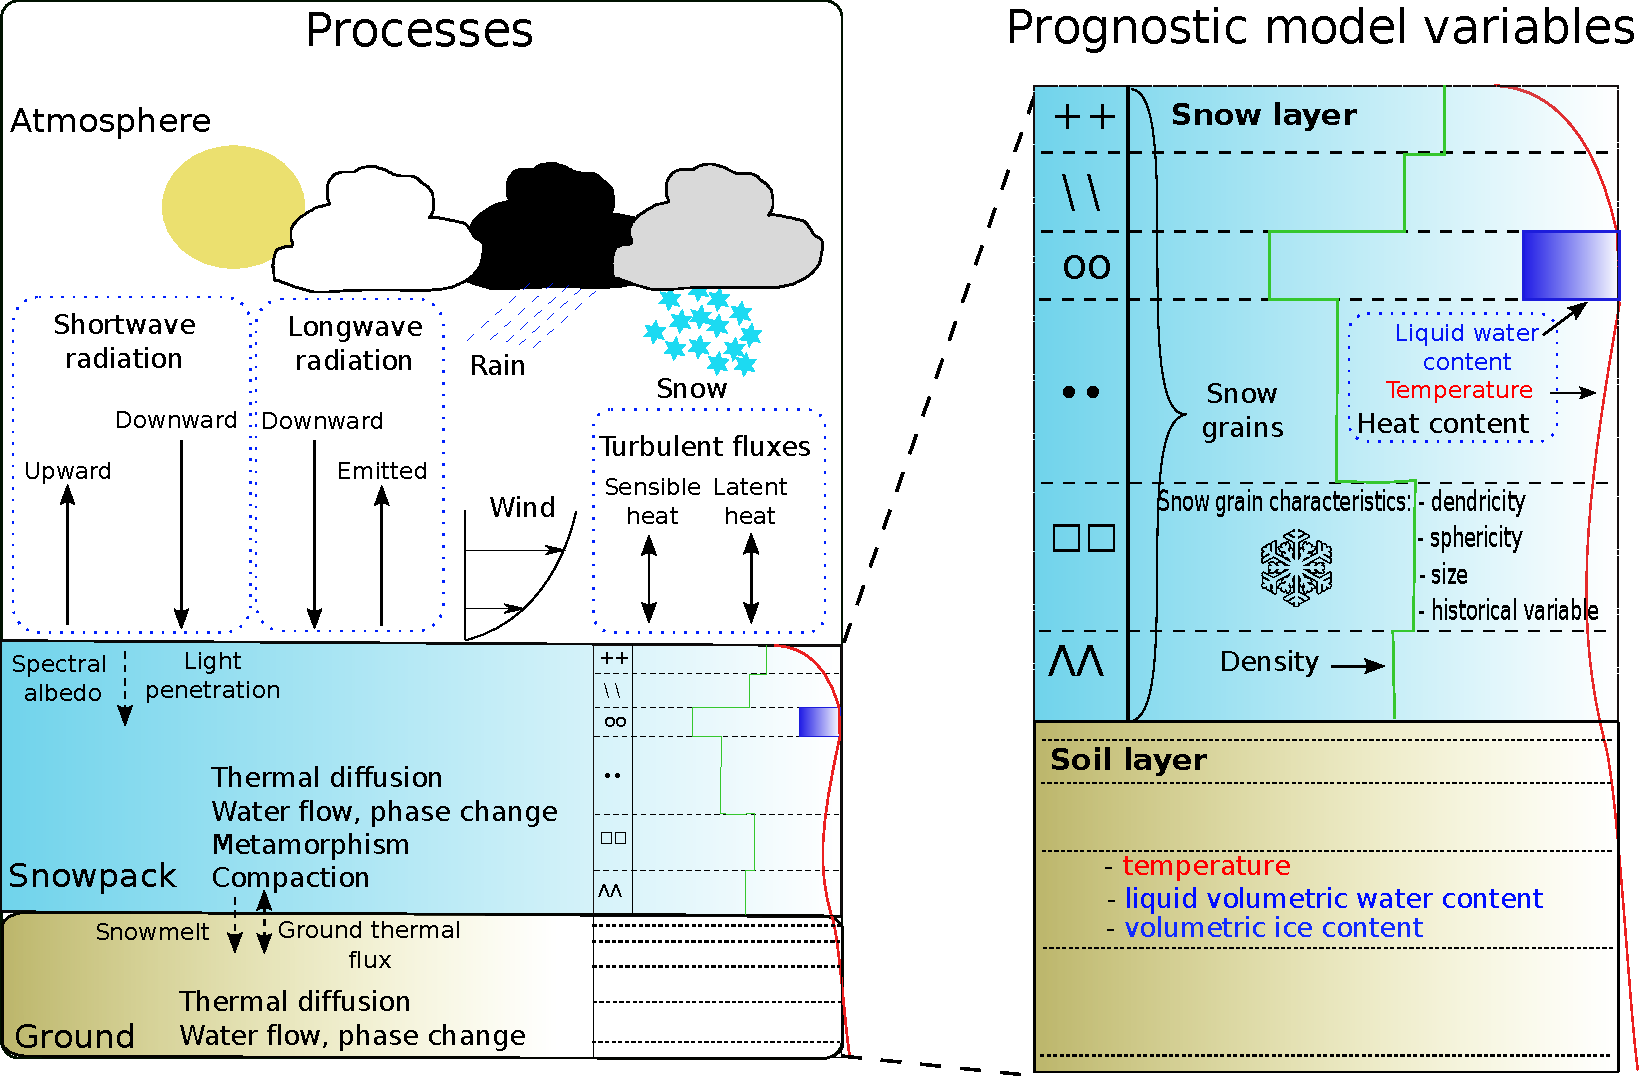
\includegraphics[width = 0.9\linewidth]{EPS/process_variables_soil.pdf}
\caption{Overview of the physical processes and prognostic variables
  used to characterize the snowpack in the multi-layer snowpack
  schemes options of ISBA (ES and Crocus). The  major differences
  between the ES and Crocus scheme is that ES does not treat snow
  metamorphism explicitly, and that the number of snow layers is kept
  significantly lower than for Crocus (on the order of 3 typically,
  vs. up to 20 or 50 for Crocus. \label{fig:schema-crocus}}
\end{center}
\end{figure}

The conservation equation for the total snow cover mass
is expressed as
%
\begin{eqnarray}
{\partial W_s \over \partial t} =
P_s + p_{sn}\,\left(P-P_s\right) - E_{s} - E_{sl} - Q_n
\,\,\,,
\end{eqnarray}
%
where $E_{sl}$ represents evaporation of liquid water
from the snow surface, and the product $p_{sn}\,\left(P-P_s\right)$
represents the portion of the total rainfall that is
intercepted by the snow surface while the remaining
rainfall is assumed to be intercepted by the snow-free soil and vegetation
canopy. The snow-runoff rate, $Q_n$,
is the rate at which
liquid water leaves the base of the snow cover.


The snow state variables are the heat content ($H_s$),
the layer thickness ($D$), and the layer average density ($\rho_s$).
The temperature ($T_{sn}$) and liquid water content ($w_{sl}$) are defined
using the heat content.
The use of the Crocus scheme induces the definition of further variables, 
which describe the morphological properties of snow grains ($d$ dendricity, $s$ sphericity, 
$g_s$ grain size, $h$ historical variable and $A$ age of a given snow layer). 
See Vionnet \etal (2012) for details.

The total snow depth, $D_s$ (m) is defined as
%
\begin{eqnarray}
D_s = \sum_{i=1}^{N_s} D_i
\end{eqnarray}
%
where a 12-layer configuration is currently used by default (i.e. $N_s=12$). 
In ES and Crocus, the thickness of the surface snow layer can be
as low as 1 mm although it typically ranges on the order of 0.01 to 0.02 m.
The thickness of internal snow layers is on the order of a
few cm typically, with a finer mesh towards the air/snow and
ground/snow interface. See Vionnet \etal (2012) and Decharme \etal
(2016) for details.

The evolution of snow density in each layer is due to snow compaction
resulting from changes in snow viscosity (Brun \etal 1989) and
wind-induced densification of near surface snow layers  
(Brun \etal 1997). This wind-driven compaction process is assumed to occur
when wind velocity exceeds a threshold value that depends on snow
surface characteristics. This process is especially important for
simulating the evolution of the snow density over polar regions. 
%
In ES, additional changes arise from snowfall which generally reduce the
snow density and more details can be seen in Decharme \etal (2016). In
Crocus, snowfall induces the creation of a new snow layer at the
surface ; mechanical settling is computed using a Newtonian formalism
where the viscosity depends mostly on the snow density and temperature
but also on the snow type (see Vionnet \etal 2012, for
details). When Crocus is used, the slope angle has an impact on the
compaction rate, since only the component of the weight perpendicular
to the snow layering need be taken into account. In practice, the
acceleration of gravity ($g=9.80665$ m s$^{−2}$) is then simply multiplied
by cos($slope_i$) where $slope_i$ is the slope of the grid point $i$.

The snow heat content (J m$^{-2}$) is defined as
%
\begin{eqnarray}
H_{s\,i} = c_{s\,i}\,D_i\,\left(T_{sn\,i}-T_0\right)
\,-\, L_f\,\rho_w \left(w_{s\,i}- w_{sl\,i}\right)\,\,\,,
\end{eqnarray}
%
where $w_s$ is the total snow layer water equivalent depth (m),
$w_{sl}$ is the snow layer liquid water content (m), and $c_s$
is the snow heat capacity (J m$^{-3}$ K$^{-1}$) (using the same
definition as the baseline ISBA snow scheme).
The snow heat content is used in order to allow
the presence of either
cold (dry) snow which has a temperature less
than or equal to the freezing point
%and contains no liquid water,
or warm (wet)
snow which is characterized by a temperature at the freezing point
and contains water in liquid form.
The snow temperature
and liquid water content can then be defined as
%
\begin{eqnarray}
T_{sn\,i} &=& T_f \,+\, \left(H_{s\,i}  + L_f\,\rho_w\,w_{s\,i}\right)
/\left(c_{s\,i}\,D_i \right) \,;
\hskip.3in
w_{l\,i} = 0 \\
%
w_{sl\,i} &=& w_{s\,i} \,+\, \left(H_{s\,i}/L_f\,\rho_w\right) \,;
\hskip1.3in
T_{sn\,i} = T_f \,\,\,{\rm and} \,\,\, w_{sl\,i} \leq w_{sl\,{\rm max}\,i}
\end{eqnarray}
%
where $w_{sl\,{\rm max}\,i}$ is the maximum liquid water
holding capacity of a snow layer,
which is based on empirical relations. All
water exceeding this flows into the layer below where
it can do one or all of the following:
add to the liquid water content, refreeze, or continue
flowing downward. 

Snow heat flow is along the thermal gradient
as any snow melt or percolated water within the snow cover
is assumed to have zero heat content.
The layer-averaged snow temperature equation
($T_{s\,i}$) is expressed as
%
\begin{eqnarray}
c_{s\,i} D_i {\partial T_{sn\,i}\over\partial t}
= G_{s\,i-1} - G_{s\,i} + R_{s\,i-1} - R_{s\,i}  - S_{s\,i}
\,\,\,,
\end{eqnarray}
%
where $S_s$ represents an energy sink/source term associated with
phase changes between the liquid and solid phases of water.
Incoming short wave radiation ($R_s$)
transmission within the snowpack decreases exponentially
with increasing snow depth. At the surface, it is expressed as
%
\begin{eqnarray}
R_{s\,0} = R_g \,\left(1-\alpha_s\right)
\end{eqnarray}
%
where the snow albedo is defined  following Brun \etal (1992). In ES
and Crocus the solar radiation is handled using three separate
spectral bands ([0.3-0.8], [0.8-1.5] and [1.5-2.8] $\mu$m). First of all,
the albedo is computed in each band, as a function of the snow
properties in the first snowpack layer for ES and the top 0.03 m of the
snowpack for Crocus. In the UV and visible range ([0.3-0.8] $\mu$m), snow
albedo depends mostly on the amount of light absorbing impurities, but
also on its micro-structure. The latter is represented by the optical
diameter of snow, $d_{opt}$, which corresponds to the diameter of a
collection of mono-dispersed ice spheres possessing the same
hemispherical albedo as the corresponding semi-infinite snow
layer. The impact of snow browning due to the deposition of light
absorbing impurities is parametrized from the age of the uppermost
snow layer. In the near-infrared bands, the spectral albedo depends
only on the optical diameter of snow. The optical diameter of
snow is currently empirically derived from the snow density and age
for ES (Decharme \etal 2016) and the microstructure properties of the
snow for Crocus (see below, and Vionnet \etal 2012). Once the
spectral albedo is calculated, in every spectral band the incoming
radiation is depleted according to the albedo value, and the remaining
part penetrates the snowpack and is gradually absorbed in the snow
layers assuming an exponential decay of radiation with depth. The
solar flux, $Q_s$, at a depth $z$ below the snow surface is expressed as
follows:
%
%%%%%%%%%%%%%%%%%%%%%%%%%%%%%%%%%%%%%%%%%%%%%%%%%%%%%%%%%%%%%%%
\begin{equation}
Q_s = SW\downarrow \, \sum^3_{k=1}
\Bigg\lbrace
\omega_k \left(1-\alpha_k\right)
{\rm exp}\left[
-\sum^i_{j=1}
\left(
\beta_{k,j}\,\Delta z_j \, 
\right)
\right]
\Bigg\rbrace
\end{equation}
%%%%%%%%%%%%%%%%%%%%%%%%%%%%%%%%%%%%%%%%%%%%%%%%%%%%%%%%%%%%%%%
%
where $SW\downarrow$ represents the incoming solar radiation, 
$\alpha_k$ the albedo and $\beta_{k,j}$ 
the absorption coefficient for the spectral band
$k$ and layer $j$. In the current version, the incoming shortwave
radiation Rs is split into three bands using empirical coefficients $\omega_k$
equal to 0.71, 0.21 and 0.08 respectively for bands [0.3-0.8], [0.8-1.5]
and [1.5-2.8] mm. Future developments will allow for forcing
where incoming shortwave radiation is partitioned into several
bands. Finally, shortwave radiation excess for thin snow cover (transmitted
through the snow) is added to the snow/ground heat flux.

The sub-surface heat ($G_s$) flux terms are evaluated using
simple diffusion. At the surface, this flux is expressed as
%
\begin{eqnarray}
G_{s\,0}
= \epsilon_s \left( R_A - \sigma_{SB} {T_{sn\,1}}^4 \right)
\,-\, H\left(T_{sn\,1}\right) \,-\, LE\left(T_{sn\,1}\right) \,-\,
c_w \,p_{sn} \left(P-P_s\right)\left(T_f-T_r\right)\,\,\,,
\end{eqnarray}
%
The last term on the right hand side of the above equation
represents a latent heat source when rain
with a temperature ($T_r$) greater than $T_0$ falls on the snow cover,
where $c_w$ represents the heat
capacity of water (4187 J kg$^{-1}$ K$^{-1}$).
Rainfall is simply assumed to have a temperature which is the larger of
the air temperature ($T_a$) and the freezing point.
The latent heat flux from the snow
includes the liquid fraction weighted
contributions from the
evaporation of liquid water and sublimation.

The ISBA surface soil/vegetation layer temperature is then
coupled to the snow scheme using
%
%%%%%%%%%%%%%%%%%%%%%%%%%%%%%%%%%%%%%%%%%%%%%%
\begin{align}
\begin{split}
{1\over C_T}{\partial T_s\over\partial t} \,\, = &\,\, 
\left(1-p_n\right) 
\left[
R_g\left(1-\alpha\right) +
\epsilon_t\left(R_A-\sigma {T_s}^4\right)- H - LE
- {2\pi \over C_T \tau} \left(T_s-T_2\right)
\right] 
\\
%
& 
\hskip.2in
\,+\, p_n \,\, \left( G_{s\,N}+R_{s\,N}
%+ c_w\,Q_n\,\left(T_f-T_s\right)
\right)
\end{split}
\end{align}
%%%%%%%%%%%%%%%%%%%%%%%%%%%%%%%%%%%%%%%%%%%%%%
%
%The term on the right hand side of the above equation
%involving the snow runoff ($Q_n$) represents an advective term.
The net surface fluxes to/from the atmosphere
are then calculated as the snow-cover
fraction weighted sums over the snow and non-snow covered
surfaces. When either multi-layer option is used (ES or Crocus), the single-layer snowpack scheme in ISBA 
is used when the snow cover is relatively thin (arbitrarily
defined as 0.05 m depth). When the snow depth exceeds this
threshold, the snow mass and heat is transferred to the chosen multi-layer
scheme. This prevents numerical difficulties
%and a more complex computer code
for vanishingly thin snow packs.

%=========================================================================================================
\subsubsection{Additional features of the Crocus scheme}
%=========================================================================================================

{\it Evolution of the vertical discretization of the finite-element grid}

The dynamical evolution of the number and thicknesses of the numerical
snow layers is a key and original feature of Crocus, which aims at
simulating  the vertical layering of natural snowpacks in the best
possible way. The maximum number of numerical layers is an important
user-defined set-up option. A minimum of 3 layers is imposed for
solving the heat conduction through the snowpack but there is no
limitation on the maximum number. As the maximum number of layers
increases, the snowpack stratigraphy can be simulated in more
detail. According to the research or operational objectives, the user
has to find the appropriate balance between the realism and the
computational cost of the simulation. An important point to mention is
that the snowpack scheme dynamically manages a different vertical grid
mesh, in terms of the number and the thickness of snow layers, for
each grid point when it is run in parallel mode for a spatially
distributed simulation ; this is a common case for snow/atmosphere
coupled simulations or for distributed stand-alone simulations. 


The adjustment of the snowpack layering is achieved with a set of
rules. The procedure is activated at the beginning of each time step
according to the following sequence:

\begin{itemize}

 \item for snowfall over a bare soil, the snowpack is built up from
   identical layers, in terms of thickness and state variables. Their
   number depends on the amount of fresh snow and on the maximum
   number of layers;

\item  for snowfall over an existing snowpack, it is first attempted
  to incorporate the freshly fallen snow into the existing top layer,
  provided its grain characteristics are similar and its thickness is
  smaller than a fixed limit. The similarity between two adjacent
  layers is determined from the value of the sum of their differences
  in terms of $d$, $s$ and $g_s$, each weighted with an appropriate
  coefficient. If the merging is not possible, a new numerical layer
  is added to the preexisting layers. If the number of layers then
  reaches its maximum, a search is carried out to identify two
  adjacent layers to be merged. This is done by minimizing a criterion
  balancing the similarity between their respective grain
  characteristics and their thicknesses;

\item for no snowfall, a check is carried out to see whether it is
  convenient to merge too thin snow layers or to split thoses which
  are thick. This is achieved by comparing the present thickness
  profile to an idealized profile, which acts as an attractor for the
  vertical grid. This idealized thickness profile depends on the
  current snow depth and on the user-defined maximal number of layers
  (see Figure \ref{fig:crocus-grid} for an example). Merging two
  layers is only possible for those which are similar enough in terms
  of grain characteristics. Grid resizing affects only one layer per
  time step, with a priority given to the surface and bottom layers,
  in order to accurately solve the energy exchanges at the surface and
  at the snow/soil interface;

\item for most time steps, no grid resizing is carried out, except
  that the thickness of each layer decreases according to its
  compaction rate.

\end{itemize}

The consistency of the physical prognostic variables is maintained in
case of grid resizing. A projection is achieved from the former
vertical grid to the new one. Mass, heat content and liquid water
content are conserved.  When a new numerical snow layer is built from
several former layers, its grain characteristics are calculated in
order to conserve the averaged weighted optical grain size of the
former layers. This insures a strong consistency in the evolution of
surface albedo, even when frequent grid resizing occur at the surface
in case of frequent snowfalls or surface melting events.


\begin{figure}[h!]
\begin{center}
%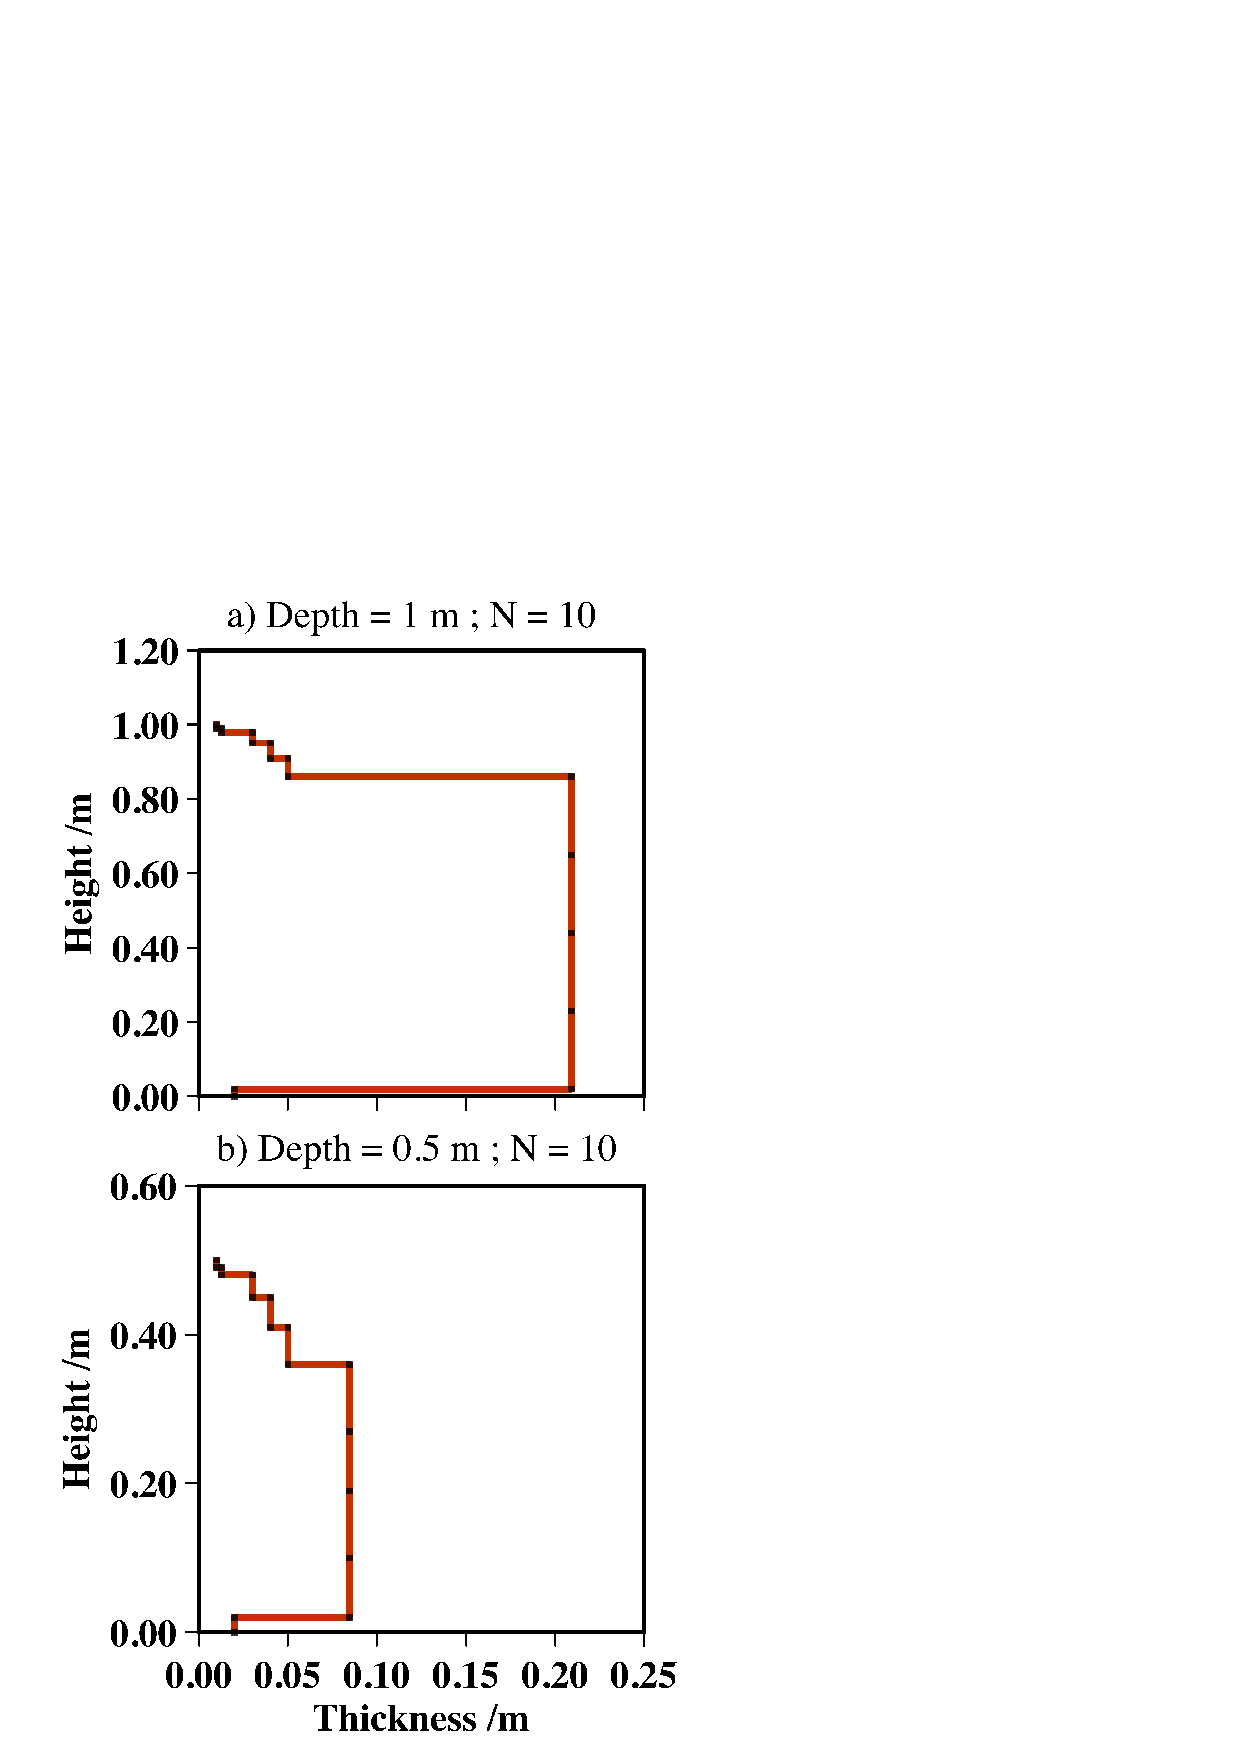
\includegraphics[width = 0.5\linewidth]{crocus-grid.pdf}
\psfig{figure=\EPSDIR/crocus-grid.eps,width=7cm}
\caption{Illustration of the optimal vertical grid of Crocus, which
  depends on total snow depth and on the user-defined maximum number
  of snow layers. \label{fig:crocus-grid}}
\end{center}
\end{figure}


{\it Snow metamorphism}

Snow metamorphism is implemented in the snowpack scheme Crocus through
a set of quantitative laws describing the evolution rate of the type
and size of the snow grains in each layer (Brun \etal 1992). This is
carried out within the subroutine. A distinction is made between
dendritic and non-dendritic snow. Snow falls as dendritic snow and
remains dendritic until $d$ reaches 0. Snow then reaches the state of
rounded crystals, faceted crystals or belongs to an intermediate
state. It is is then characterized by its sphericity ($s$), ranging
from 0 to 1, and a grain size, $g_s$, ranging from 0.3 to 0.4 mm. Such
snow is defined as non-dendritic. The metamorphism laws that govern
the evolution of snow grain depend on temperature, the temperature
gradient, and include wet metamorphism. They are similar to the laws
initially described by Brun \etal (1992) and are mostly based on
empirical fits to experimental data. The metamorphism laws that govern
the evolution of snow grain are given in Table~\ref{tab_metamo_dry}
and~\ref{tab_metamo_wet}, respectively for dry and wet
metamorphism. In the case of temperature gradient metamorphism, fits
to experimental data by Marbouty (1980)\nocite{marbouty1980} are
used. In this case, the increase of grain size $g_s$ follows:
%
\begin{equation}
\frac{\delta g_s}{\delta t} = f(T)h(\rho)g(G)\Phi
\end{equation}
where G is the absolute value of the temperature gradient $(|\delta T
/ \delta z|)$ and $f$, $g$, $h$ and $\Phi$ are dimensionless functions
varying from 0 to 1 given by:
%
\begin{equation}
f = \left\{
    \begin{array}{ll}
       0 & \mbox{if}\quad T-T_{\rm fus}  < -40~\mathrm{K} \\
       0.011\times(T-T_{\rm fus}+40) & \mbox{if} \quad -40\le T-T_{\rm fus}< -22~\mathrm{K}  \\
       0.2+0.05\times(T-T_{\rm fus}+22) & \mbox{if} \quad -22\le T-T_{\rm fus}< -6~\mathrm{K}  \\     
       1-0.05\times(T-T_{\rm fus})&\mbox{otherwise}
    \end{array}
\right.
\label{eqn_fmarb}
\end{equation}
where $T_{\rm fus}$  is temperature of the melting point for water (K), and $h$, $g$ and $\Phi$ are given below:
\begin{equation}
\Phi = 1.0417.10^{-9}~\mathrm{m\,s}^{-1}
\label{eqn_phimarb}
\end{equation}
\begin{equation}
h = \left\{
    \begin{array}{ll}
       1.& \mbox{if}\quad\rho < 150 \quad \mbox{kg\,m}^{-3}\\
       1-0.004\times(\rho-150) & \mbox{if}\quad 150<\quad\rho < 400 \quad \mbox{kg\,m}^{-3}\\     
       0.& \mbox{otherwise}
    \end{array}
\right.
\label{eqn_hmarb}
\end{equation}
\begin{equation}
g = \left\{
    \begin{array}{ll}
       0. & \mbox{if}\quad G < 15~\mathrm{K\,m}^{-1} \\
       0.01\times(G-15) & \mbox{if} \quad 15\le G< 25~\mathrm{K\,m}^{-1}  \\
       0.1+0.037\times(G-25) & \mbox{if} \quad 25\le G< 40~\mathrm{K\,m}^{-1} \\   
       0.65+0.02\times(G-40) & \mbox{if} \quad 40\le G< 50~\mathrm{K\,m}^{-1} \\
       0.85+0.0075\times(G-50) & \mbox{if} \quad 50\le G< 70~\mathrm{K\,m}^{-1} \\    
       1. &\mbox{otherwise}
    \end{array}
\right.
\label{eqn_gmarb}
\end{equation}


\begin{table}[t]
\caption{Metamorphism laws under dry conditions. G is the vertical temperature gradient $(|\delta T / \delta z|) $, $T$ the temperature (K) and $t$ is time expressed in days. $f$, $g$, $h$ and $\Phi$ are empirical functions to predict depth-hoar growth-rate from Marbouty (1980).}
\vskip4mm
\centering
\begin{tabular}{c|c|c}
\hline
&Non-dendritic snow &Dendritic snow \\
\hline
\multirow{2}{*}{ $G$ $\leq$ 5 K.m$^{-1}$} & $\frac{\delta s}{\delta t} = 10^9e^{-6000/T}$ & $\frac{\delta d}{\delta t} = -2.10^8e^{-6000/T}$ \\
& $\frac{\delta g_s}{\delta t} = 0$ &$\frac{\delta s}{\delta t} = 10^9e^{-6000/T}$ \\
%\middlehline
\hline
\multirow{2}{*}{5 $<$ $G$ $\leq$ 15 K.m$^{-1}$} & $\frac{\delta s}{\delta t} = -2.10^8e^{-6000/T}G^{0.4}$ &\multirow{2}{*}{$\frac{\delta d}{\delta t} = -2.10^8e^{-6000/T} G^{0.4}$} \\
& $\frac{\delta g_s}{\delta t} = 0$ &\\
\cline{1-2}
\multirow{2}{*}{$G$ $>$ 15 K.m$^{-1}$} & if $s>$0: $\frac{\delta s}{\delta t} = -2.10^8e^{-6000/T}G^{0.4}$ and $\frac{\delta g_s}{\delta t} = 0$ & \multirow{2}{*}{$\frac{\delta s}{\delta t} = -2.10^8e^{-6000/T} G^{0.4}$} \\
& if $s=$0: $\frac{\delta s}{\delta t} = 0$ and $\frac{\delta g_s}{\delta t} = f(T)h(\rho)g(G)\Phi$ & \\
\hline
\end{tabular}
\label{tab_metamo_dry}
\end{table}

\begin{table}[t]
\caption{Metamorphism laws in the presence of liquid water. $\theta$ is the mass liquid water content and $t$ is time expressed in days. $v$ refers to the equivalent volume of snow grain and $v'_0$ and $v'_1$ are empirical constants taken from Brun (1989).}
\vskip4mm
\centering
\begin{tabular}{c|c|cc}
\cline{1-3}
\cline{1-3}
&Non-dendritic snow &Dendritic snow & \\
\cline{1-3}
\multirow{2}{*}{0 $\leq$ $s$ $<$ 1} & $\frac{\delta g_s}{\delta t} = 0$ & \multirow{2}{*}{ $\frac{\delta d}{\delta t} = -\frac{1}{16} \theta^3$ }&  \\
& $\frac{\delta s}{\delta t} = \frac{1}{16} \theta^3$ & &with $ \theta = 100\frac{W_{\rm liq}}{\rho D}$\\
\cline{1-2}
\multirow{2}{*}{$s$ $=$ 1} & $\frac{\delta s}{\delta t} = 0$ &\multirow{2}{*}{$\frac{\delta s}{\delta t} = \frac{1}{16} \theta^3$} &\\
& $\frac{\delta v}{\delta t} = v'_0+v'_1 \theta^3$ && \\
\cline{1-3}
\end{tabular}
\label{tab_metamo_wet}
\end{table}

In addition to this default metamorphism formulations, three other formulations 
of metamorphism can be activated. The first one (C13) is similar to the default 
one but uses the optical diameter and the sphericity as prognostic variables. 
The second one (T07) is based on the parameterizations from Taillandier \etal (2007)
\nocite{taillandier2007}%\citet{Taillandier2007} 
and Domine \etal (2007) \nocite{domine2007}%\citet{Domine2007}
and the last one (F06) is based on the parameterizations 
from Flanner \etal (2006) \nocite{flanner2006}.%\citet{Flanner2006}
For detail of these implementations please refer to Carmagnola \etal (2014) 
\nocite{Carmagnola2014}.%\citet{Carmagnola 2014}

{\it Snow radiative transfer scheme}

In addition to the basic formation of solar energy absorption and snow albedo 
over three spectral bands described above, a new option is available for solar 
radiative transfer calculation in the snowpack. The radiative scheme is called 
TARTES Libois \etal (2013) \nocite{libois2013}%\citep{Libois2013} 
(Two-streAm Radiative TransfEr in Snow model). TARTES 
is a two-stream radiative transfer scheme based on an analytical formulation of 
radiative transfer in snow (Kokhanovsky \etal (2004))\nocite{kokhanovsky2004}.
%\citep{Kokhanovsky2004}
TARTES computes spectral  solar absorption within each layer and diagnoses spectral 
and broadband albedo. The default spectral resolution is 20 nm. The scheme uses 
spectral solar irradiance calculated from input broabdand data using a parameterization 
derived from SBDART (Ricchiazzi \etal (1998))\nocite{ricchiazzi1998} %\citep{Richiazzi1998} 
at Col de Porte site. The scientific documentation of TARTES is available at 
http://lgge.osug.fr/~picard/tartes/. 

TARTES simulates the effect of light absorbing impurities as an equivalent 
black-carbon content. To this respect, three options can be activated :

\begin{itemize}
\item "TA1": no impurity
\item "TA2":  snow impurity content constant to 100 ng g$^{-1}$
\item "TAR" : impurity content = 2*snow age ng g$^{-1}$
\end{itemize} 

{\it Effects of wind}

{\bf{
			\begin{center}
			\begin{tabular}{|l|}
\hline
 \textcircled{!} As a 1D model, the continental surface scheme ISBA within SURFEX is \\
 NOT designed to handle explicitly wind-induced snow redistribution. \\
 Indeed, grid points are treated independently from each other. \\
 Nevertheless, the Crocus snowpack scheme includes parameterizations \\
 that represent some effects of wind drift on the snowpack.  \\
\hline
			\end{tabular}
			\end{center}

}}

The compaction and the metamorphism of the surface layers during wind
drift events are taken into account in a simplified way, as described
initially by Brun \etal (1997). A mobility index, $M_{\rm O} $,
describes the potential for snow erosion for a given snow layer and
depends on the microstructural properties of snow ($d$, $s$ and
$g_s$):
%
\begin{equation}
M_{\rm O} = \left\{
    \begin{array}{ll}
       0.34\left( 0.75 d-0.5s+0.5 \right) + 0.66F(\rho) & \mbox{dendritic case}\\
       0.34\left( -0.583 g_s-0.833s+0.833 \right) + 0.66 F(\rho)& \mbox{non-dendritic case}
    \end{array}
\right.\\
\label{eqn_mobindex}
\end{equation}
where $F(\rho)=\left[1.25-0.0042 \left(
    \mathrm{max}(\rho_{min},\rho)-\rho_{min} \right)\right]$ and
$\rho_{min}=50$ kg\,m$^{-3}$. The expression for $M_{\rm O}$ in
Eq.~\ref{eqn_mobindex} combines the parameterization of Guyomarc'h and
Merindol (1998)\nocite{guyomarch1998} (first term) developed for
alpine snow with a term depending on snow density ($F(\rho)$). The
purpose is to extend the use of $M_{\rm O}$ to polar snow which has a
density generally larger than 330 kg\,m$^{-3}$ (upper limit for
application of Guyomarc'h and Merindol, 1998). Fresh snow (high
values of $d$, low value of $\rho$) presents high values of mobility
index which tend to decrease with time due to sintering (increase of
$s$) and compaction (increase of $\rho$). Guyomarc'h and Merindol
(1998) combined the mobility index with wind speed, $U$, to compute a
so-called "driftability" index, $S_I$:
%
\begin{equation}
S_I = -2.868 \exp (-0.085U)+1+M_{\rm O}
\label{eqn_drifindex}
\end{equation}
Positive values of $S_I$ indicate that snow drifting can occur while
$S_I = 0$ gives the value of the threshold wind speed for snow
transport. During a drift event, blown snow particles in saltation
break upon collision with the snow surface and tend towards rounded
grains (Clifton \etal (2006)\nocite{Clifton2006}). For a given snow
layer $i$, a time characteristic for snow grain change under wind
transport is computed:
%
\begin{equation}
\tau_i = \frac{\tau}{\Gamma_{i~{\rm drift}}} \quad \mathrm{where}~\Gamma_{i~{\rm drift}} = \mathrm{max}[0,S_{Ii}\exp(-z_i/0.1)]
\label{eqn_to}
\end{equation}
%
where $\tau$ is empirically set to 48 hours. The pseudo-depth in the
snow pack, $z_i$ (in m, positive downwards), takes into account
previous hardening of snow layers $j$ situated above the current layer
$i$: 
%
%%%%%%%%%%%%%%%%%%%%%%%%%%%%%%%%%%%%%%%%%%%%%%%%%%%%%%%%%%%%%%%%%%%%%%%%%%%%%
\begin{equation}
z_i = \sum_j \left[ D_j \times \left(3.25-S_{Ij} \right) \right]  
\end{equation}
%%%%%%%%%%%%%%%%%%%%%%%%%%%%%%%%%%%%%%%%%%%%%%%%%%%%%%%%%%%%%%%%%%%%%%%%%%%%%
%
Therefore, through the
variable $\Gamma_{\rm drift}$, compaction and rounding rates in a snow
layer depends on the grain driftability and are propagated to the
layers below with an exponential decay until it reaches a
non-transportable layer ($S_I\le$0). Compaction and rounding rates are
detailed in Table~\ref{tab_evol_drift}.



\begin{table}[t]
\caption{Evolution rates of snow grain properties and density in layer
  $i$ caused by snow drifiting. $t$ is time expressed in hours and
  $\tau$ represents the time characteristic for snow grains change
  under wind transport given by Eq.~\ref{eqn_to}.}  
\vskip4mm
\centering
\begin{tabular}{c|c|c}
\hline
Parameters&Non-dendritic snow &Dendritic snow \\
\hline
\multirow{2}{*}{Grain properties} & $\frac{\delta s}{\delta t} = \frac{1-s}{\tau}$  & $\frac{\delta d}{\delta t} = \frac{d}{2\tau}$ \\
& $\frac{\delta g_s}{\delta t} = \frac{5.10^{-4}}{\tau} $ & $\frac{\delta s}{\delta t} = \frac{1-s}{\tau}$\\
%\middlehline
\hline
Snow density &    \multicolumn{2}{c}{ $\frac{\delta \rho}{\delta t} =\frac{\rho_{\rm max}-\rho}{\tau}$ with $\rho_{\rm max} =350$ kg\,m$^{-3}$ }\\
\hline
\end{tabular}
\label{tab_evol_drift}
\end{table}

As an option and in case of snow drifting, Crocus computes the
associated rate of sublimation according to a parameterization
developed by Gordon \etal (2006)\nocite{Gordon2006}. This
parameterization allows the estimation of the sublimation rate in a
column of blowing or drifting snow, combining existing
parameterizations from Schmidt \etal (1982)\nocite{schmidt1982},
Bintanja \etal (1998)\nocite{bintanja1995} and  D\'{e}ry \etal
(2001)\nocite{dery2002}. The total sublimation rate of blowing snow
$Q_s$ depends on the near-surface meteorological conditions according
to: 
%
\begin{equation}
Q_s=A(\frac{T_0}{T_a})^\gamma U_t\rho_aq_{si}(1-Rh_i)(\frac{U}{U_t})^B
\end{equation}
where $T_a$ is the air temperature ($K$), $T_0$ a constant with a
value of 273.16 K, $U$ the wind speed, $U_t$ the threshold wind speed
for snow transport, $\rho_a$ the air density and $Rh_i$ the relative
humidity with respect to ice. $q_{si}$ denotes the saturation specific
humidity (kg/kg) at temperature $T_a$. $\gamma$, $A$ and $B$ are
dimensionless parameters with values $4.0$, $0.0018$ and $3.6$,
respectively. $U_t$ is the threshold wind speed for wind
transportation, obtained by setting $S_I$ = 0. in equation
(\ref{eqn_drifindex}):
%
\begin{equation}
U_t = -\frac{\log\left((M_{\rm O}+1.)/2.868 \right)}{0.085}
\end{equation}
Using this option, Crocus subtracts the corresponding mass from the snowpack surface at each model timestep.

%=========================================================================================================
%=========================================================================================================
\subsection{The surface fluxes}
%=========================================================================================================
%=========================================================================================================

Only one energy balance is considered for the whole system
ground-vegetation-snow (when the 3-layer snow scheme option is not in use).
As a result, heat and mass transfers between the surface and
the atmosphere are related to the mean values $T_s$ and $w_g$.

The net radiation at the surface is the sum of the absorbed
fractions of the incoming solar radiation $R_G$ and of the
atmospheric infrared radiation $R_A$, reduced by the emitted
infrared radiation:
\begin{eqnarray} \label{eqnRN}
R_n = R_G (1-\alpha_t) + \epsilon_t \left( R_A-\sigma_{SB}{T_s}^4 \right)
\end{eqnarray}
where $\sigma_{SB}$ is the Stefan-Boltzmann constant.

The turbulent fluxes are calculated by means of the classical
aerodynamic formulas.  For the sensible heat flux:
\begin{eqnarray}
H = \rho_a c_p C_H V_a (T_s - T_a) \label{eqnH}
\end{eqnarray}
where $c_p$ is the specific heat; $\rho_a$, $V_a$, and $T_a$
are, respectively, the air density, the wind speed, and the
temperature at the lowest atmospheric level; and $C_H$,
as discussed below, is the
drag coefficient depending upon the thermal stability of the
atmosphere. The explicit snow scheme sensible heat flux
is calculated using the same formulation (but with $T_{sn}$).
The water vapor flux $E$ is the sum of the evaporation
of liquid water
from the soil surface (i.e., $E_{g\,l}$), from the vegetation (i.e., $E_v$),
and sublimation from the snow and soil ice (i.e, $E_s$ and $E_{g\,f}$):
%
\begin{eqnarray}
LE &=& LE_{g\,l} + LE_v + L_i \left(E_s + E_{g\,f}\right) \\
E_{g\,l} &=& (1-veg)(1-p_{sng})\left(1-\delta_i\right)\, \rho_a C_H V_a
        \left( h_u q_{sat}(T_s) - q_a \right) \label{eqnLEG} \\
E_v &=& veg (1-p_{snv}) \rho_a C_H V_a h_v
        \left( q_{sat}(T_s) - q_a \right) \\
E_s &=& p_{sn} \rho_a C_H V_a
        \left( q_{sat}(T_s) - q_a \right) \\
E_{g\,f} &=&
\,\left(1-veg\right)\left(1-p_{sng}\right)\,\delta_i\, \rho_a C_H V_a
\left( h_{ui} \,q_{\rm sat}\left(T_s\right) \,-\, q_a \right)
\end{eqnarray}
where $L$ and $L_i$ are the specific heat of evaporation
and sublimation, $q_{sat}(T_s)$ is the saturated
specific humidity at the
temperature $T_s$, and $q_a$ is the atmospheric specific humidity
at the lowest atmospheric level. The snow fractions $p_{sn}$ and
$p_{snv}$
are defined by Eq.s~\ref{eq:isba_snow_frac_total} 
and \ref{eq:isba_snow_frac_veg}, respectively.
%
The water vapor flux $E$
from the explicit snow surface is expressed as
%
\begin{eqnarray}
LE\left(T_{sn\,1}\right) &=& L E_{sl} + L_i E_s \\
E_{sl} &=& \delta_{sn} \,\rho_a C_{Hs} V_a
        \left( q_{sat}\left(T_{sn\,1}\right) - q_a \right) \\
E_s &=& \left(1-\delta_{sn}\right) \,
        \rho_a C_{Hs} V_a \left( q_{sat}\left(T_{sn\,1}\right) - q_a \right) \\
\delta_{sn} &=& w_{sl\,1}/w_{sl\,{\rm max}\,1}\,;
\hskip2.2in
0 \leq \delta_{sn} \leq 1
\end{eqnarray}
%
where evaporation of liquid water is zero when $T_{sn\,1}<T_0$.
The transfer coefficient ($C_{Hs}$) is calculated over the snow
covered surface using the same formulation as $C_H$.

The surface ice fraction is
is used to partition the bare soil latent heat flux
between evaporation and sublimation, and it is defined as
%
%%%%%%%%%%%%%%%%%%%%%%%%%%%%%%%%%%%%%%%%%%%
\begin{equation}
\label{eq:isba_soil_froz_frac}
\delta_i = w_{g\,f}/\left(w_{g\,f}+w_g\right) \,;
\hskip.5in
0 \leq \delta_i < 1   \,\,\,.
\end{equation}
%%%%%%%%%%%%%%%%%%%%%%%%%%%%%%%%%%%%%%%%%%%

The relative humidity $h_u$ at the ground surface is related to the
superficial soil moisture $w_g$ following
%
%%%%%%%%%%%%%%%%%%%%%%%%%%%%%%%%%%%%%%%%%%%%%%%%%%
\begin{equation}
%
h_u \,\, = \,\, \Bigg\lbrace
%
\begin{matrix}
{1 \over 2} \left[ 1- {\rm cos}\left( {w_g \over {w_{fc}}^\ast} \pi \right)\right] 
&
\hskip.25in w_g < {w_{fc}}^\ast 
\\
1 
&
\hskip.25in w_g \geq {w_{fc}}^\ast
\end{matrix}
\end{equation}
%%%%%%%%%%%%%%%%%%%%%%%%%%%%%%%%%%%%%%%%%%%%%%%%%%%
%
where the field capacity with respect to the liquid water
is defined using the modified soil porosity so
that ${w_{fc}}^\ast = w_{fc}\,w_{sat}^\ast/w_{sat}$.
The humidity for the ice covered portion of the grid box
is calculated in a similar fashion as
%
%%%%%%%%%%%%%%%%%%%%%%%%%%%%%%%%%%%%%%%%%%%%%%%%%%
\begin{equation}
%
h_{ui} \,\, = \,\, \Bigg\lbrace
%
\begin{matrix}
{1 \over 2} \left[ 1-cos \left( {w_{g\,f} \over {w_{fc}}^{\ast\ast}}
    \pi \right)\right] 
& \hskip.25in w_{g\,f} < {w_{fc}}^{\ast\ast} 
\\
1 
& \hskip.25in w_{g\,f} \geq {w_{fc}}^{\ast\ast}
\end{matrix}
\end{equation}
%%%%%%%%%%%%%%%%%%%%%%%%%%%%%%%%%%%%%%%%%%%%%%%%%%%
%
where ${w_{fc}}^{\ast\ast} = w_{fc}(w_{sat}-w_g)/w_{sat}$.
In case of dew flux when $q_{sat}(T_s) < q_a$, $h_u$ is also set
to 1 (see Mahfouf and Noilhan (1991)\nocite{Mahfouf1991a} for details).
When the flux $E_v$ is positive, the Halstead coefficient $h_v$
takes into account the direct evaporation $E_r$ from the fraction
$\delta$ of the foliage covered by intercepted water, as well as
the transpiration $E_{tr}$ of the remaining part of the leaves:
%
%%%%%%%%%%%%%%%%%%%%%%%%%%%%%%%%%%%%%%%%%%%%%%%%%%%%%%%%%%%
\begin{align}
\label{eq:isba_halstead}
h_v    =& (1-\delta) R_a / (R_a+R_s) + \delta 
\\
E_r    =& veg(1-p_{snv}) {\delta \over R_a}
        \left[ q_{sat} (T_s) - q_a \right] 
\\
E_{tr}=& veg(1-p_{snv}) {1-\delta \over R_a + R_s}
           \left[ q_{sat}(T_s) - q_a \right] 
\end{align}
%%%%%%%%%%%%%%%%%%%%%%%%%%%%%%%%%%%%%%%%%%%%%%%%%%%%%%%%%%%
%
When $E_v$ is negative, the dew flux is supposed to occur
at the potential rate, and $h_v$ is taken equal to 1.
%
%Following Deardorff (1978), $\delta$ is a power function of the
%moisture content of the interception reservoir:
%\begin{eqnarray}
%\delta = (W_r / W_{rmax})^{2/3}
%\end{eqnarray}


The aerodynamic resistance is $R_a = ( C_H V_a )^{-1}$.
The surface resistance, $R_s$, depends upon both atmospheric
factors and available water in the soil; it is given by:
\begin{eqnarray}
R_s = {R_{smin} \over F_1 F_2 F_3 F_4 LAI}
\end{eqnarray}
with the limiting factors $F_1$, $F_2$, $F_3$, and $F_4$:
\begin{eqnarray}
F_1 &=& {f+R_{smin}/R_{smax} \over 1+f} \\
F_2 &=& {w_2-w_{wilt} \over w_{fc} - w_{wilt} } \ \ \ \
and \ 0 \leq F_2 \leq 1 \\
F_3 &=& 1 - \gamma \left( q_{sat}(T_s) - q_a \right) \\
F_4 &=& 1-1.6\times 10^{-3} (T_a - 298.15)^2
\end{eqnarray}
where the dimensionless term $f$ represents the incoming
photosynthetically active radiation on the foliage,
normalized by a species-dependent threshold value:
\begin{eqnarray}
f = 0.55 {R_G \over R_{Gl}} {2 \over LAI}
\end{eqnarray}
Moreover,
$\gamma$ is a species-dependent parameter (see Jacquemin and Noilhan (1990)\nocite{Jacquemin1990}) and $R_{smax}$ is arbitrarily set to $5000 \ s m^{-1}$.

The surface fluxes of heat, moisture, and momentum can
be expressed as
\begin{eqnarray}
(\overline{w'\theta'})_s &=& {H \over \rho_a c_p T_a / \theta_a} \label{eqn_H} \\
(\overline{w'r'_v})_s &=& {E \over \rho_a (1-q_a)} \label{eqn_LE} \\
|\overline{w'V'}|_s &=& C_D |V_a|^2  = u^2_* \label{eqn_FM}
\end{eqnarray}
where $r_v$ is the water vapor mixing ratio,
$w$ is the vertical motion, $\theta_a$ is the potential
temperature at the lowest atmospheric level.  The primes and
overbars denote perturbation and average quantities.

For the drag coefficients $C_H$ and $C_D$, the formulation of
Louis (1979)\nocite{Louis1979} was modified in order to consider different
roughness length values for heat $z_0$ and momentum $z_{0h}$
(Mascart \etal (1995)\nocite{Mascart1995}):
%
%%%%%%%%%%%%%%%%%%%%%%%%%%%%%%%%%%%%%%%%%%
\begin{align}
\label{eq:isba_drag_transfer_coef}
C_D &= C_{DN} F_m 
\\
\label{eq:isba_heat_transfer_coef}
C_H &= C_{DN} F_h
\end{align}
%%%%%%%%%%%%%%%%%%%%%%%%%%%%%%%%%%%%%%%%%%
%
with
%
%%%%%%%%%%%%%%%%%%%%%%%%%%%%%%%%%%%%%%%%%%%%%%
\begin{equation}
\label{eq:isba_drag_transfer_coef_neutral}
C_{DN} = \frac{k^2 }{ \left[ {\textrm{ln}} \left( z / z_0\right) \right]^2} 
\end{equation}
%%%%%%%%%%%%%%%%%%%%%%%%%%%%%%%%%%%%%%%%%%%%%%
%
where $k$ is the Von Karmann constant.  Also
\begin{eqnarray}
F_m &=& 1 - {10 Ri \over 1 + C_m
        \sqrt{|Ri|} }  \ \ \ \ \ if \ Ri \leq 0 \\
F_m &=& {1 \over 1 + {10Ri \over \sqrt{1+5Ri}}} \
        \ \ \ \ \ \ \ \ \ \ \ \ \ if \ Ri > 0
\end{eqnarray}
and
\begin{eqnarray}
F_h = \left[ 1-{15Ri \over 1 + C_h \sqrt{|Ri|}} \right]
      \times \left[ {ln(z/z_{0}) \over ln(z/z_{0h})} \right] \
      \ \ \ \ \ \ \ \ if \ Ri \leq 0 \\
F_h = {1 \over 1+15Ri \sqrt{1+5Ri}}
      \times \left[ {ln(z/z_{0}) \over ln(z/z_{0h})} \right] \
      \ \ \ \ \ \ \ \ if \ Ri > 0
\end{eqnarray}
where $Ri$ is the gradient Richardson number.
The coefficients $C_m$ and $C_h$ of the unstable case are given by
\begin{eqnarray}
C_m &=& 10 {C_m}^* C_{DN} (z/z_{0})^{p_m} \\
C_h &=& 15 {C_h}^* C_{DN} (z/z_{0h})^{p_h} \times
        \left[ {ln(z/z_{0}) \over ln(z/z_{0h})} \right]
\end{eqnarray}
where $C^*_m$, $C^*_h$, $p_m$, and $p_h$ are functions of the ratio
$\mu = ln(z_{0}/z_{0h})$ only:
\begin{eqnarray}
C^*_h &=& 3.2165 + 4.3431 \times \mu + 0.5360 \times \mu^2
        - 0.0781 \times \mu^3 \\
C^*_m &=& 6.8741 + 2.6933 \times \mu - 0.3601 \times \mu^2
        + 0.0154 \times \mu^3 \\
p_h &=& 0.5802 - 0.1571 \times \mu + 0.0327 \times \mu^2
        - 0.0026 \times \mu^3 \\
p_m &=& 0.5233 - 0.0815 \times \mu + 0.0135 \times \mu^2
        - 0.0010 \times \mu^3
\end{eqnarray}


%=========================================================================================================
%=========================================================================================================
\subsection{ISBA-Multi-Energy-Budget (MEB) Explicit Vegetation}
\label{sec:isba_meb}
%=========================================================================================================
%=========================================================================================================

ISBA includes an option to represent forests (using the corresponding
patches) using the Multi-Energy-Budget (ISBA-MEB) explicit vegetation
scheme (Boone et al., 2017; Napoly et al., 2017)
\nocite{boone_ea_2017,napoly_ea_2017}.
%
MEB is based on the classic two-source model for snow-free conditions
which considers explicit energy budgets (for computing fluxes and
effective surface temperatures)
for the soil and the vegetation, and it has been extended to a
three-source model in order to include an explicit representation
of snowpack processes and their interactions with the ground and
the vegetation.
%
The vegetation canopy is represented
using the so-called big-leaf method which lumps
the entire vegetation canopy into a single effective leaf
for computing energy budgets and the associated fluxes of heat,
moisture and momentum.
%
One of the first examples of a two-source model designed for
atmospheric model studies is 
Deardorff (1978)\nocite{Deardorff1978}, 
and further refinements to the vegetation canopy
processes were added in the years that followed leading to
fairly sophisticated schemes 
which are similar to those used today (e.g. Sellers et al., 1986)
\nocite{Sellers86}.
%Such models have also been coupled to detailed multi-layer soil
%models \citep[e.g.,][]{Braud_ea_1995}.
%
The two-source big-leaf approach 
(e.g. Braud et al., 1995)
\nocite{Braud_ea_1995}
has been used extensively
within coupled regional and global scale land-atmosphere models 
(Xue et al., 1991; Sellers et al., 1996; Dickinson et al., 1998;
Lawrence et al., 2011; Saluelsson et al., 2011)
\nocite{Xue91,Sellers96,Dickinson1998,Lawrence2011,Samuelsson11}.
%
Some key features of MEB compared to the default 
ISBA treatment of
forests are:

\begin{itemize}

\item seperate ground (surface) and vegetation canopy energy
  budgets. This is in contrast to the single composite soil-vegetation
  energy budget in ISBA. This permits the estimation of 
  a more realistic surface radiative temperature, and surface flux
  partitioning. 

\item a snow fraction which can gradually bury the vegetation
  vertically thereby transitioning the turbulence and radiative 
  coupling from the
  snow to the canopy air space to that between the snow and
  the atmosphere. Note that this differs from the notion of
  the vegetation snow cover fraction, $p_{nv}$, of the ISBA composite scheme.

\item the detailed solar radiation transfer scheme  
%%from ISBA-Ags 
  which is a multi-layer model that
  considers two spectral bands, direct and diffuse
  flux components and the concept of sunlit and shaded leaves 
  Carrer et al. (2013)\nocite{carrer_ea_2013}.
%and was developed to improve the modeling of photosynthesis within
%ISBA
  It is used when ISBA-Ags is active: for MEB it is always used.

\item a detailed treatment of canopy snow interception and
  unloading processes and a coupling
  with the ISBA physically-based multi-layer snow scheme.

%\item a reformulation of the turbulent exchange coefficients within the
%canopy air space for stable conditions, such as over a snowpack

%\item a fully implicit Jacobean matrix for the longwave fluxes from
%multiple surfaces (snow, below-canopy snow-free ground surface,
%vegetation canopy)

\item an explicit forest litter layer model (which also acts as the
  below-canopy surface energy budget when litter covers the soil)

\item seperate ground surface and vegetation surface properties
  (roughness lengths, albedo, emissivity...). Note that the composite
  surface notion of $veg$ is dropped in MEB.

\end{itemize}
\noindent
%
All of the energy budgets are
numerically implicitly coupled with each other and with the atmosphere
using the coupling method adapted from Best et al. (2004)
\nocite{Best2004} 
which was
first proposed by Polcher et al. (1998)
\nocite{Polcher1998}.

Currently, forests make
up 8 patches for the 19-class option, and three for the 12-class
option.
ISBA-MEB (referred to hereafter
simply as MEB) 
option can be
activated for any number of the forest patches.
%
By default, MEB is coupled to the multi-layer soil (DF)
(Boone et al., 2000; Decharme et al., 2011)
\nocite{Boone2000,Decharme2011}, 
and snow (ES) schemes 
(Boone et al., 2001; Decharme et al., 2016)
\nocite{Boone2001,Decharme16}.
MEB can also be
coupled to the simple 3-layer soil 
Force-Restore (3-L) option 
(Boone et al., 1999)
\nocite{Boone1999} 
in order to be compatible
with certain applications which have historically used 3-L, but by
default, it is
coupled with DF since the objective is to move towards a less
conceptual (more explicit process-based) LSM.

A schematic diagram for a maximum illustrating
the various resistance pathways for the turbulent fluxes for 
the three fully (implicitly) coupled surface energy budgets
is shown in Fig.~\ref{fig:schematic_meb}. The water budget
prognostic variables are also indicated.
%
There are six aerodynamic resistance, $R_{a}$ (m s$^{-1}$), pathways which
are indicated in red and defined as being between; 
i) the non-snow buried vegetation canopy and the canopy air, 
$R_{a\,vg-c}$, 
ii) the non-snow buried ground surface (soil or litter) and the canopy air,
$R_{a\,g-c}$,
iii) the snow surface and the canopy
air, $R_{a\,n-c}$, 
iv) the ground-based snow-covered part of the canopy 
and the canopy air, $R_{a\,vn-c}$,
v) the canopy air with the overlying atmosphere, $R_{a\,c-a}$), 
and vi) the ground-based snow surface (directly) with 
the overlying atmosphere, $R_{a\,n-a}$.
%
Previous papers describing ISBA 
(Noilhan and Planton, 1989; Noilhan and Mahfouf, 1996)
\nocite{Noilhan1989,Noilhan1996}
expressed heat fluxes using a dimensionless heat and mass exchange coefficient,
$C_H$:
however for the new MEB option, it is more convenient to express the different
fluxes using resistances (s m$^{-1}$)
which are related to the exchange coefficient as
$R_a=1/\left(V_a\,C_H\right)$.

%%%%%%%%%%%%%%%%%%%%%%%%%%%%%%%%%%%%%%
%\vskip.25in
\begin{figure}[!b]
\centerline{ 
%\includegraphics[angle=270, width=8cm]{figs/schematic_gv_n.eps}
%\includegraphics[angle=0, width=10cm]{FIGURES/schematic_g_v_ng_na.eps}}
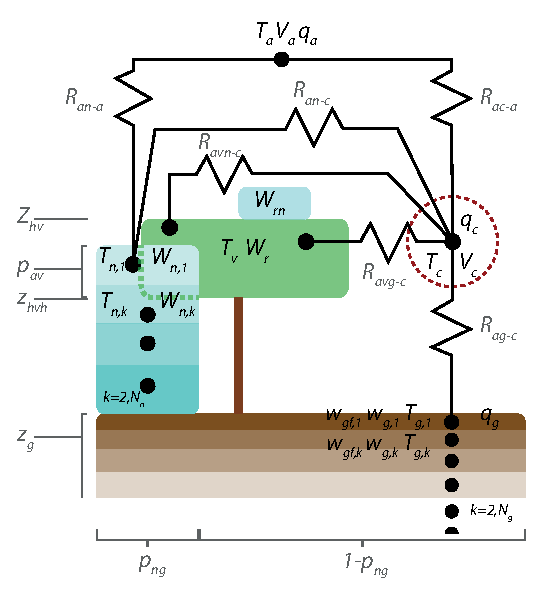
\includegraphics[angle=0, width=10cm]{EPS/schematic_g_v_ng_na_colorfill.eps}}
\caption{
A schematic representation of 
%the composite soil-vegetation
%ISBA scheme with an explicit snowpack (ISBA-ES): left-hand side.
%The ISBA-MEB schematic is shown on the right.
the turbulent aerodynamic resistance, $R_{a}$, pathways for
ISBA-MEB. The prognostic temperature, liquid water, and liquid water
equivalent variables are shown.
The canopy air diagnostic variables are enclosed by the red-dashed circle.
The ground-based snow pack is indicated using
turquoise, the vegetation canopy is shaded green,
and ground layers are colored brown.
Atmospheric variables (lowest atmospheric 
model or observed reference level) are indicated using
the $a$ subscript.
The ground snow fraction, $p_{ng}$ (note, this corresponds to
$p_{sng}$ in the text), and canopy-snow-cover 
fraction, $p_{n\alpha}$, are indicated.
}
\label{fig:schematic_meb}
\end{figure}
%%%%%%%%%%%%%%%%%%%%%%%%%%%%%%%%%%%%%%


The surface energy budgets are formulated in terms of prognostic
equations for the temperature evolution of the bulk vegetation canopy, $T_v$, 
the snow-free ground surface (soil or litter), $T_g$, and the
ground-based
snowpack, $T_n$ (K). The prognostic hydrological variables
are: the liquid soil volumetric water content, $w_g$ (m$^3$ m$^{-3}$),
liquid water equivalent volumetric
ice content, $W_{gf}$ (m$^3$ m$^{-3}$), snow water equivalent
(SWE), $W_n$,
vegetation canopy intercepted liquid water, $W_r$, and intercepted
snow, $W_{rn}$ (kg m$^{-2}$).  
%
The diagnosed variables which are determined implicitly during the
simultaneous solution of the energy budgets are; 
%colored in dark red;
the surface specific humidity at saturation 
for each of the three energy budgets, $q$ (kg
kg$^{-1}$), and the canopy air specific humidity, $q_c$, temperature,
$T_c$ and wind speed, $V_c$ (m s$^{-1}$).
%
The surface snow cover fraction
area is represented by $p_{sng}$ as in the (baresoil part of the) 
composite version of ISBA, 
while the fraction of the canopy
buried by the ground-based snowpack is defined as $p_{\alpha n}$
%(the snow fraction parameterizations 
%are described in Section~\ref{sec:snow_frac}.)
%
%Finally, 
The snowpack has $N_n$ layers, while the number of soil
layers is defined as $N_g$ where $k$ is the vertical index (increasing
from 1 at the surface downward). The ground and snowpack uppermost
layer temperatures 
correspond to those used for the surface energy budget (i.e. $k=1$).
%

%=========================================================================================================
\subsubsection{Snow Fractions}
\label{sec:snow_frac} 
%=========================================================================================================

%Snow is known to
%have a significant impact on heat conduction fluxes owing to
%it's relatively high insulating properties. In addition, it can significantly
%reduce turbulent transfer owing to reduced surface roughness, and it
%has a relatively large surface albedo thereby impacting the surface net
%radiation budget. Thus, the parameterization of it's areal coverage
%turns out to be a critical aspect of LSM modeling of snowpack-atmosphere
%interactions and sub-surface soil and hydrological processes. 
%
The fractional ground coverage by the snowpack, $p_{sng}$, 
is defined from Eq.~\ref{eq:isba_snow_frac_ground}.
%
%%%%%%%%%%%%%%%%%%%%%%%%%
%\begin{equation}
%\label{eq:meb_png}
%p_{sng} = W_n/W_{n,crit}
%\hskip1.in
%\left( 0 \leq p_{sng} \leq 1 \right)
%\end{equation}
%%%%%%%%%%%%%%%%%%%%%%%%%
%
%where currently 
The suggested value for the critical snow water equivalent (at which
coverage is unity) for MEB
is currently $W_{crn}=1$ (kg m$^{-2}$).
Note that this is considerably lower than the previous value of 10 kg m$^{-2}$
used in ISBA 
(Douville et al., 1995)
\nocite{DOUVILLE1995a}, 
but this value has been shown to improve the ground soil
temperatures  using an explicit snow scheme within 
ISBA 
Brun et al. (2013)\nocite{brun_2012}.

Note that for MEB, the ISBA snow fraction over vegetation, 
$p_{snv}$ (Eq.~\ref{eq:isba_snow_frac_veg}), 
is not used since it is
more consistent with a composite surface.
The fraction of the vegetation canopy which is buried by ground-based snow
which is deamed to be more consistent with a forest canopy structure
is defined as 
%
%%%%%%%%%%%%%%%%%%%%%%%%%
\begin{equation}
\label{eq:meb_LAIcansnow}
p_{n\alpha} = 
\frac
{\left(D_n - z_{hv,b}\right)}
{\left(z_{hv} - z_{hv,b}\right)}
\hskip1.25in
\left( 0 \leq  p_{n\alpha} \leq 1\right)
\end{equation}
%%%%%%%%%%%%%%%%%%%%%%%%%
%
where $D_n$ is the total ground-based snowpack depth (m), 
%$z_{hv}$ is defined as the top of the vegetation canopy (m), 
and $z_{hvb}$
represents the base of the vegetation canopy (m) 
(see Fig.~\ref{fig:forest_snow_MEB}) which is currently defined as
%
%%%%%%%%%%%%%%%%%%%%%%%%%%
\begin{equation}
\label{eq:meb_pn_alphan}
z_{hvb} = a_{hv}\,\left(z_{hv} - z_{hv,min}\right)
\hskip1.in
\left(z_{hvb} \geq 0\right)
%
\end{equation}
%%%%%%%%%%%%%%%%%%%%%%%%%%%
%
where $a_{hv}=0.2$ and the effective canopy base height is
set to $z_{hv,min}=2$ (m) for forests. The foliage distribution
should be reconsidered in further development since literature
suggests
(e.g. Massman, 1982)\nocite{Massman1982}, 
that the foliage is not
symmetrically distributed in the crown but skewed upward.



%%%%%%%%%%%%%%%%%%%%%%%%%%%%%%%%%%%%%%
%\vskip.25in
\begin{figure}[!b]
\centerline{ 
%\includegraphics[angle=0, width=12cm, clip=true, trim=1cm 7cm 1cm 8cm]{FIGURES/forest_snow_MEB_sketch.eps}}
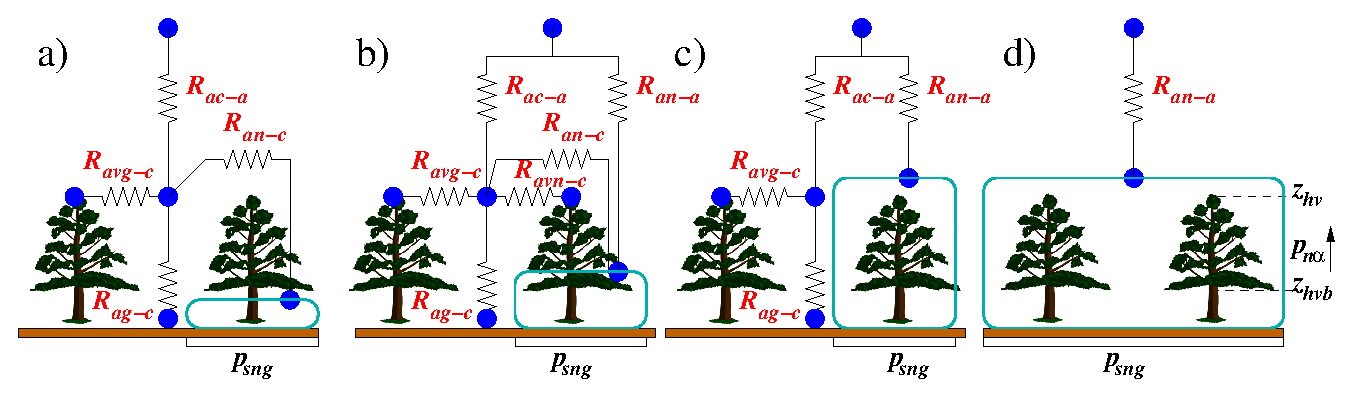
\includegraphics[angle=0, width=14cm, clip=true]{EPS/tree_resistance.eps}}
\caption{
A schematic sketch illustrating the role of $p_{n\alpha}$, the fraction of the vegetation
canopy which is buried by ground-based snow. In panel a), the snow is well
below the canopy base, $z_{hvb}$, 
resulting in $p_{n\alpha}=0$ and the snow has no direct energy exchange with the atmosphere.
In panel b), the canopy is partly buried by snow ($0<p_{n\alpha}<1$) and the snow has energy exchanges
with both the canopy air and the atmosphere.
In panel c), the canopy is fully buried by snow ($p_{n\alpha}=1$) and the snow has energy exchange
only with the atmosphere while the soil and canopy only exchange with
the canopy air space ($p_{sng}<1$). Finally, in panel d), both
$p_{sng}=1$ and $p_{n\alpha}=1$, so
that the only exchanges are between the snow and the atmosphere.
}
\label{fig:forest_snow_MEB}
\end{figure}
%%%%%%%%%%%%%%%%%%%%%%%%%%%%%%%%%%%%%%


%=========================================================================================================
\subsubsection{Energy Budget}
\label{sec:meb_energy_budget}
%=========================================================================================================

The coupled energy budget equations for a three-source model
can be expressed for a single bulk canopy, a ground-based snowpack and a 
underlying ground surface as
%
%%%%%%%%%%%%%%%%%%%%%%%%%
\begin{align}
\label{eq:meb_cvdtvdt_three}
{\cal C}_v {\frac {\partial T_v}{\partial t}} =& 
R_{n\,v} - H_{v} - LE_{v} 
\,+\, L_f\,\Phi_{v} 
\\
%
\label{eq:meb_cgdtgdt_three}
{\cal C}_{g,1} {\frac {\partial T_{g,1}}{\partial t}} =& 
\left(1-p_{sng}\right) \left( R_{n\,g} - H_{g} - LE_{g}\right)
\,+\, p_{sng}\left(G_{gn} + \tau_{n,N_n}SW_{n\,n}\right)
\,-\, G_{g,1} \,+\, L_f\,\Phi_{g,1} 
\\
%
\label{eq:meb_cndtndt_three}
%p_{sng}\, 
{\cal C}_{n,1} {\frac {\partial T_{n,1}}{\partial t}} =& 
%\left( 
R_{n\,n} - H_{n} - LE_{n} - \tau_{n,1}SW_{n\,n} 
\,+\, \xi_{n,1} \,-\, G_{n,1} \,+\, L_f\,\Phi_{n,1} 
%\right) p_{sng} 
%
\end{align}
%%%%%%%%%%%%%%%%%%%%%%%%%
%
where $T_{g,1}$ is the uppermost ground (surface soil or litter layer) temperature,
$T_{n,1}$ is the surface snow temperature, 
and $T_v$ is the bulk-canopy temperature (K). 
%
Note that the subscript 1
indicates the uppermost layer or the base of the layer (for fluxes) 
for the soil and snowpack.
% (vegetation is
%treated as a single bulk layer, thus there is no indexing).
%$L_f$ represents the latent heat of fusion, and
%$LE$ represents the various latent heat flux terms.
%$L$ represents the effective latent heat (J kg$^{-1}$)
%(more details are given in Appendix~\ref{app:turb_flux_expressions}).
%The subscript for the turbulent fluxes is defined using the same convention
%as for aerodynamic resistances (Section~\ref{sec:model_descrip}).
%surface-atmosphere: $g-c$ implies ground to canopy
%air space, $v-c$ repsesents vagatation canopy to canopy
%air space, and $n-N$ implies snow surface to the overlying
%atmosphere (the center-level of the $N$th layer of the atmospheric model, just above the surface: we sometimes 
%also use the subscript $a$ 
%to represent this level).
%
The ground-based snow fraction is defined as $p_{sng}$. 
Note that the terms of Eq.~\ref{eq:meb_cgdtgdt_three} are multiplied by
$p_{sng}$ to make them patch-relative (or grid-box relative in the case
of single-patch mode) since the snow can potentially cover only part of the
patch. Within the snow module itself, the notion of
$p_{sng}$ is not used (the computations are snow-relative). 
%The formulation for $p_{sng}$ is described in 
%Section~\ref{sec:snow_frac}.
But note that when simultaneously solving the
coupled equations
Eq.s~\ref{eq:meb_cvdtvdt_three}-\ref{eq:meb_cndtndt_three}, 
Eq.~\ref{eq:meb_cndtndt_three} must be multiplied by $p_{sng}$ since
snow only covers a fraction
of the area to make the snow patch-relative: further details are given
in Section~\ref{sec:meb_discret_ebud}. 

The phase change terms (freezing less melting: expressed in kg m$^{-2}$ s$^{-1}$) 
terms for the snow water equivalent intercepted by the vegetation
canopy, 
the uppermost ground layer, and the uppermost snowpack layer are
represented by
$\Phi_{v}$,  $\Phi_{g,1}$ and $\Phi_{n,1}$, respectively.
$L_f$ represents the latent heat of fusion (J kg$^{-1}$).
%
The computation of $\Phi_{g,1}$ uses the Gibbs free-energy method
(also note that $\Phi_{g,1}=\Phi_{f,1}-\Phi_{m,1}$: see Section~\ref{sec:isba_soil_ice}), 
$\Phi_{n,1}$ is based on available liquid for freezing or cold
content for freezing 
(see Section~\ref{sec:isba_multi_layer_snow})
%(Boone and Etchevers, 2001)\nocite{Boone2001},
and $\Phi_{v}$ is described herein (see Eq.~\ref{eq:meb_sn2w}).
%
%$LE$ represents the various latent heat flux terms.
Note that all of the phase change terms are computed as adjustments
to the surface temperatures (after the fluxes have been computed),
therefore only the energy storage terms (and not the fluxes) 
are modified directly by phase
changes for each model time step.
%
The last term on the RHS of Eq.~\ref{eq:meb_cndtndt_three}, 
$\xi_{n,1}$, represents the effective heating or cooling
of a snowpack layer caused by exchanges in enthalpy between the
surface and sub-surface model
layers 
when the vertical grid is reset (the snow model grid layer thicknesses vary in time). 

%-----------------------------------------------------------------------------------------------------
%
%The heat capacity (J m$^{-3}$ K$^{-1}$) of each layer is expressed using $c$, while
%$D_{n,k}$ and $\Delta z_{g,k}$ represent the snow and soil layer thicknesses (m), respectively.
%The ${\cal C}$ terms represent the special case for the surface for $k=1$. 
%%They
%%are analogous to the inverse of the
%%Force-Restore thermal inertia coefficients. 
%%Note that if there is no understory vegetation, then ${\cal C}_g=c_{g,1}\Delta z_{g,1}$, while for 
%%snow, ${\cal C}_n=c_{n,1} D_{n,1}$ always. 
The surface ground, snow,
and vegetation
effective heat capacities, ${\cal C}_{g,1}$, ${\cal C}_v$ and 
${\cal C}_{n,1}$ (J m$^{-2}$ K$^{-1}$)
are defined, respectively, as
%
%The values for the soil and the vegetation are defined as
%
%%%%%%%%%%%%%%%%%%%%%%%%%
\begin{align}
\label{eq:meb_cvdtvdtn_sfc_g_hcaps}
%
{\cal C}_{g,1} = & 
\Delta z_{g,1}\, c_{g,1}\
%\frac{1}{ p_{ff}/C_f \,+\, 
%\left(1-p_{ff}\right)/
%\left( \Delta z_{g,1}\, c_{g\,i}\right)}
%
%\hskip.5in & \left( {\cal C}_{g,1} \geq {\cal C}_{g,min}\right)
%\\
%\label{eq:meb_cvdtvdtn_sfc_n_hcaps}
%
\\
\label{eq:meb_cvdtvdtn_sfc_v_hcaps}
%
{\cal C}_{v} = & C_{vb} \,+\, C_i \, W_{r,n} \,+\, C_w \, W_r
%
%& \left( {\cal C}_{v} \geq {\cal C}_{v,min}\right)
\\
\label{eq:meb_cvdtvdtn_sfc_n_hcaps}
%
{\cal C}_{n,1} = & D_{n,1}\,c_{n,1}
\end{align}
%%%%%%%%%%%%%%%%%%%%%%%%%
%
%The flooded fraction, $p_{ff}$ is discussed in more detail in
%Sect.~\ref{sec:water_budget}.
%
where
$C_i$ and $C_w$ are the specific
heat capacities for solid 
($2.106 \times 10^3$ J kg$^{-1}$ K$^{-1}$) 
and liquid water ($4.218 \times 10^3$ J kg$^{-1}$ K$^{-1}$), respectively.
%
The uppermost ground layer thickness is $\Delta z_{g,1}$ (m),
and the corresponding heat capacity of this layer is defined as
$c_{g\,1}$ (J m$^{-3}$ K$^{-1}$). 
%
%The uppermost soil layer ranges between 0.01
%and 0.03 m for most applications, so that the interactions between
%surface fluxes and fast temperature changes in the surface soil layer
%can be represented.
%
There are two options for modeling the thermal properties of the
uppermost ground layer.
%
First, they ($c_{g\,1}$ and $\lambda_{g\,1}$)
can be defined using the default ISBA configuration for a soil layer 
with parameters based on soil texture properties
which can also incorporate
the thermal effects of soil organics
(Decharme et al., 2016)\nocite{Decharme16}: see Section~\ref{sect:isbacc_soil}.
%
The second option, 
which is the default when using MEB,
is to model the uppermost ground layer as forest litter.
This means using values of $c$, $\lambda$ and $\Delta z$ 
which correspond to litter to compute ${\cal C}$
in Eq.~\ref{eq:meb_cvdtvdtn_sfc_g_hcaps}
(Napoly et al., 2017)\nocite{napoly_ea_2017}:
see Section~\ref{sec:meb_litter} for details. 
%
%See Napoly et al. (2016)\nocite{napoly_ea_2016} 
%for a detailed description of this scheme
%and it's impact on the surface energy budget.

%
%%%%%%%%%%%%%%%%%%%%%%%%%%
%\begin{equation}
%\label{eq:meb_cvdtvdtn_sfc_g_soil}
%c_{g\,i} = \left(1-w_{sat,i}\right) C_{g,i} \,+\, C_l \,\rho_l \,w_{g,i} 
%\,+\, C_i \,\rho_i \, w_{gf,i}
%%
%\end{equation}
%%%%%%%%%%%%%%%%%%%%%%%%%
%
%where $w_{g}$ and $w_{gf}$ represent the volumetric liquid water and liquid water
%equivalent soil water contents (m$^{3}$ m$^{-3}$), respectively (see Sect.\ref{sec:water_budget}
%for their governing equations). The density of liquid water and ice
%(assumed to have a constant value of 920 kg m$^{-3}$) are defined by $\rho_l$
%and $\rho_i$, respectively. The soil porosity is represented by $w_{sat}$.
%
The canopy is characterized by low heat capacity which means that its temperature responds
fast to changes in fluxes. Thus, to realistically simulate diurnal variations in 2-meter temperature
this effect must be accounted for.
Sellers et al. (1986)\nocite{Sellers86} 
defined the value as
being the heat capacity of 0.2 kg m$^{-2}$ of water per unit leaf area
index ($LAI$: m$^{2}$ m$^{-2}$). This results in values on the order of $1\times 10^{4}$ J
m$^{-2}$ K$^{-1}$ for forest canopies in general. 
%
%The canopy acts more or less
%like a cover above the ground surface, therefore, it is really the temperature and specific humidity conditions
%in the canopy air space, $T_{c}$ and $q_{c}$, that set the conditions for heat fluxes between canopy, ground surface,
%and lowest model level. 
%
For local scale simulations, $C_{vb}$ can be defined based on
observational data.
In spatially distributed simulations (or when observational data is
insufficient), $C_{vb} = 0.2/C_{V,ref}$
where the vegetation thermal
inertia, $C_{V,ref}$ is defined as a function of vegetation class by the
SURFEX default physiographic database ECOCLIMAP
(Faroux \etal, 2013)\nocite{faroux2013}. 
%
Note that $C_V$ has been determined for the composite
soil-vegetation scheme, so the factor 0.2 is used to reduce this value
to be more representative of vegetation and on the order of the
value discussed by Sellers et al. (1986)\nocite{Sellers86}.
Numerical tests have shown that using this value, the canopy
heat storage is on the order of 10 W m$^{-2}$ at mid-day for a typical
mid-latitude summer day for a forest.
%
The minimum vegetation heat capacity value is limited at
$1\times 10^{4}$ (J m$^{-2}$ K$^{-1}$)
in order to model, in a rather simple fashion, 
the thermal inertia of stems, branches, trunks, etc.
%In fact, 
%there is not much model sensitivty to this
%parameter (i.e. futher phase shifts and amplitude increases) 
%for lower values except that numerical problems can arise for large time
%steps. Thus, this value reduces the potential for oscillations or
%shocks in $T_v$, and at the same time takes into account plant biomass
%in the absence of leaves.
%
The contributions from intercepted snow and rain are incorporated,
where $W_{r,n}$ and $W_r$ (kg m$^{-2}$) represent the 
equivalent liquid water content of
intercepted canopy snow and liquid water, respectively. 
%
The uppermost snow layer thickness is $D_{n,1}$ (m), and the
corresponding heat capacity is represented by $c_{n,1}$ 
(see Section~\ref{sec:isba_multi_layer_snow} for details on the
explicit snow scheme variables).
%(Boone and Etchevers, 2001)\nocite{Boone2001}. 
%Note that $D_{n,1}$ is limited to
%values no larger than several centimeters in order to model a
%reasonable thermal inertia (i.e. in order to represent the diurnal
%cycle) in a fashion analogous to the soil.
%For more details, see 
%Decharme et al. (2016)\nocite{Decharme16}, 
%
The numerical solution of the surface energy budget,
sub-surface soil and snow temperatures, and the implicit numerical
coupling with the atmosphere is described in 
Appendix~\ref{app:meb_numerical_soln}.

%=========================================================================================================
\subsubsection{Turbulent fluxes}
\label{sec:meb_energy_budget_turb}
%=========================================================================================================

In this section, the turbulent heat and water vapor fluxes 
in Eq.s~\ref{eq:meb_cvdtvdt_three}-\ref{eq:meb_cndtndt_three} are described.

%-------------------------------------------------------------------------------------
%\subsubsection{Sensible heat fluxes}
%\label{sec:energy_budget_turb_h}



The MEB sensible heat fluxes are defined as
%
%%%%%%%%%%%%%%%%%%%%%%%%%
\begin{align}
\label{eq:meb_sens_veg}
H_{v} =& \rho_a \,
{\frac{\left( {\cal T}_v - {\cal T}_c \right)}{R_{a\,v-c}}}
\\
%
\label{eq:meb_sens_grnd}
H_{g} =& \rho_a \,
%\left(1-p_{sng}\right) \,
{\frac{\left( {\cal T}_g - {\cal T}_c \right)}{R_{a\,g-c}}} 
\\
%
\label{eq:meb_sens_snow}
H_{n} =& \rho_a \,
\left[
\left(1-p_{n\alpha}\right)
\, 
{\frac{\left( {\cal T}_n - {\cal T}_c \right)}{R_{a\,n-c}}} 
\,+\,
p_{n\alpha}
\, 
{\frac{\left( {\cal T}_n - {\cal T}_a \right)}{R_{a\,n-a}}}  
\right]
\\
%
\label{eq:meb_sens_ca}
H_{c} =& 
\rho_a \,{\frac{\left( {\cal T}_c - {\cal T}_a \right)}{R_{a\,c-a}}} 
\\
%
\label{eq:meb_sens_all}
%H =& 
%\left(1-p_{n\alpha}\, p_{sng}\right)\, H_{c}
%\,+\,
%p_{n\alpha}\, p_{sng}\, H_{n-a}
H =& \rho_a \,
\left[
\left(1-p_{n\alpha}\, p_{sng}\right)
\, 
{\frac{\left( {\cal T}_c - {\cal T}_a \right)}{R_{a\,c-a}}} 
\,+\,
p_{n\alpha}\, p_{sng}
\, 
{\frac{\left( {\cal T}_n - {\cal T}_a \right)}{R_{a\,n-a}}} 
\right]
%
\end{align}
%%%%%%%%%%%%%%%%%%%%%%%%%
%
where $\rho_a$ represents the lowest atmospheric layer average air
density (kg m$^{-3}$).
The fluxes between the canopy air space and  
the vegetation, $H_v$, the snow-free ground, $H_g$, and the ground-based
snowpack, $H_n$, 
%are defined by 
%Eq.s~\ref{eq:meb_sens_veg}-\ref{eq:meb_sens_snow}, 
%respectively.
%These fluxes 
appear in the surface energy budget equations 
(Eq.s\ref{eq:meb_cvdtvdt_three}-\ref{eq:meb_cndtndt_three}).
%
The sensible heat flux from the ground-based snowpack (Eq.~\ref{eq:meb_sens_snow}) 
is partitioned by the fraction of the vegetation which is buried by the
ground-based snowpack, $p_{n\alpha}$, 
between an exchange between the canopy air space,
%$H_{n-c}$, 
and the overlying atmosphere
(Eq.~\ref{eq:meb_LAIcansnow}).
%
The heat flux between the overlaying atmosphere and the canopy air
space is represented by $H_c$, and it is equivalent to the sum of
the fluxes between the different energy budgets and the canopy air
space.
%
The total flux exchange between the
overlying atmosphere and the surface (as seen by the atmosphere) 
is defined by $H$.
It is comprised of two components: the heat exchange between the
overlying atmosphere and the canopy air space 
and the part of the ground-based snowpack 
which is burying the vegetation.
%
%It is convenient to split $H_{n}$ into two components since one
%governs the coupling between the canopy air space and the snow
%surface, while the other modulates the exchanges with the overlying
%atmosphere (as the canopy layer becomes buried).
%
%Using 
%the definition of the total canopy resistance, $R_{a\,v-c}$ (Eq.~\ref{eq:resis}),
%the canopy heat flux, $H_v$ (Eq.~\ref{eq:sens_veg}) can be split into
%the sensible heat fluxes from the partially snow-buried and snow-free
%canopy:
%
%%%%%%%%%%%%%%%%%%%%%%%%%%
%\begin{align}
%\label{eq:sens_veg_vn}
%H_{vn} =& \rho_a \,
%\left( {\cal T}_v - {\cal T}_c \right)
%\left[
%{\frac{\left(1-p_{n\alpha}\right)\,p_{sng}}{R_{a\,vn-c}}}
%\right]
%\\
%
%\label{eq:sens_veg_vg}
%H_{vg} =& \rho_a \,
%\left( {\cal T}_v - {\cal T}_c \right)
%\left[
%{\frac{\left(1-p_{sng}\right)}{R_{a\,vg-c}}} 
%\right]
%
%\end{align}
%%%%%%%%%%%%%%%%%%%%%%%%%
%
The ground-based snowpack heat flux, $H_n$ (Eq.~\ref{eq:meb_sens_snow}), 
can be split into a part which modulates the
heat exchange
with the canopy air space, $H_{n-c}$ and the other part which 
controls the exchanges directly with the overlying atmosphere,
$H_{n-a}$, defined as
%
%%%%%%%%%%%%%%%%%%%%%%%%%%
\begin{align}
%
\label{eq:meb_sens_snow_canopy_n}
H_{n-c} =& \rho_a \,
\, 
{\frac{\left( {\cal T}_n - {\cal T}_c \right)}{R_{a\,n-c}}} 
%
\\
\label{eq:meb_sens_snow_atmos_a}
H_{n-a} =& \rho_a \,
{\frac{\left( {\cal T}_n - {\cal T}_a \right)}{R_{a\,n-a}}}  
\end{align}
%%%%%%%%%%%%%%%%%%%%%%%%%
%
${\cal T}_c$ is diagnosed by imposing conservation of the heat fluxes
between the surface and the canopy air (As described in
Appendix~\ref{app:meb_numerical_soln}).
%
Using the definition in Eq.~\ref{eq:meb_sens_snow_atmos_a},
the total sensible heat flux exchange with the atmosphere 
(Eq.~\ref{eq:meb_sens_all})
can also be written in more compact form as
%
%%%%%%%%%%%%%%%%%%%%%%%%
\begin{equation}
H = \rho_a \left[
\left(1-p_{sng}\,p_{n\alpha}\right) \, H_c
\,+\,
p_{sng}\,p_{n\alpha} \, H_{n-a}
\right]
\end{equation}
%%%%%%%%%%%%%%%%%%%%%%%%
%
%This method has been developed to model the covering of
%low vegetation canopies 
%or shrubs 
%by a ground-based snowpack.
%
%%%%%%%%%%%%%%%%%%%%%%%%%
%\begin{align}
%
%\label{eq:meb_sens_snow_canopy}
%H_{n-c} =& \rho_a \,
%\, 
%{\frac{\left( {\cal T}_n - {\cal T}_c \right)}{R_{a\,n-c}}} 
%
%\\
%\label{eq:meb_sens_snow_atmos}
%H_{n-a} =& \rho_a \,
%{\frac{\left( {\cal T}_n - {\cal T}_a \right)}{R_{a\,n-a}}}  
%\end{align}
%%%%%%%%%%%%%%%%%%%%%%%%%
%
%
%$C_p$ is the specific heat capacity of dry air (J kg$^{-1}$ K$^{-1}$),
%
Finally, the final fluxes for the given patch are aggregated using
$p_{sng}$ and $p_{n\alpha}$.
%: the full expressions are given 
%in Appendix~\ref{sensible_heat_fluxes}.


The total canopy aerodynamic resistance is comprised 
of snow-buried, $R_{a\,vn-c}$, and non-snow buried, $R_{a\,vg-c}$, 
resistances from
%
%%%%%%%%%%%%%%%%%%%%%%%%%%
\begin{equation}
\label{eq:meb_resis}
R_{a\,v-c} = 
{\left[
{\frac{\left(1-p_{n\alpha}\right)\,p_{sng}}{R_{a\,vn-c}}}
\,+\, 
{\frac{\left(1-p_{sng}\right)}{R_{a\,vg-c}}} 
\right]}^{-1}
%
\end{equation}
%%%%%%%%%%%%%%%%%%%%%%%%%%%
%
%
The separation of the resistances is done to mainly account for differences
in the roughness length between the buried and non-covered parts of
the vegetation canopy, so
the primary effect of snow cover is to increase the resistance
relative to a snow-free surface assuming the same temperature gradient
owing to a lower surface roughness, thus $R_{a\,vn-c} \geq R_{a\,vg-c}$.
%
The formulation also provides a continuous
transition to the case of vanishing canopy turbulent fluxes 
as the canopy becomes entirely buried
(as $p_{n\alpha}\rightarrow 1$).
%
In this case,
the energy budget 
equations collapse into a simple coupling
between the snow surface and the overlying atmosphere, and
the ground energy budget is simply consists in
heat conduction between the ground surface and the snowpack base.
%
%Note that the canopy aerodynamic resistance 
%$R_{a\,v-c} \rightarrow R_{a\,vg-c}$
%as $p_{n\alpha}\rightarrow 0$.
%
%
%The sensible flux between the canopy air space and the overlying
%atmosphere, $H_c$, is defined as the sum of the heat exchanges between
%the surface and the canopy air as
%
%%%%%%%%%%%%%%%%%%%%%%%%%
%\begin{equation}
%\label{eq:meb_sens_ca}
%H_{c} = p_{sng}\,H_{n-c} \,+\, \left(1-p_{sng}\right)\,H_{g}\,+\, H_{v} 
%\,\, = \,\, 
%\rho_a \,{\frac{\left( {\cal T}_c - {\cal T}_a \right)}{R_{a\,c-a}}} 
%\end{equation}
%%%%%%%%%%%%%%%%%%%%%%%%%
%
%
The formulations of the resistances between the different surfaces and
the canopy airspace and the overlying atmosphere are 
described in detail in 
Sect.~\ref{sec:meb_resistances}.
%
The canopy air temperature, which is needed by different physics
routines, 
is diagnosed
by combining Eq.~s\ref{eq:meb_sens_veg}-\ref{eq:meb_sens_all}
and solving for ${\cal T}_c$ and using
Eq.~\ref{eq:meb_thermo_var} to determine $T_c$
(see Eq.~\ref{eq:meb_canopy_air_t_update}).
%(see Appendix~\ref{app:thermo_var} for details).
%
%Finally, the total sensible heat flux exchange with the atmosphere is 
%defined as
%
%%%%%%%%%%%%%%%%%%%%%%%%%
%\begin{equation}
%\label{eq:meb_sens_all}
%H = 
%\left(1-p_{n\alpha}\, p_{sng}\right)\, H_{c}
%\,+\,
%p_{n\alpha}\, p_{sng}\, H_{n-a}
%
%H =& \rho_a \,
%\left[
%\left(1-p_{n\alpha}\, p_{sng}\right)
%\, 
%{\frac{\left( {\cal T}_c - {\cal T}_a \right)}{R_{a\,c-a}}} 
%\,+\,
%p_{n\alpha}\, p_{sng}
%\, 
%{\frac{\left( {\cal T}_n - {\cal T}_a \right)}{r_{a\,n-a}}} 
%\right]
%
%\end{equation}
%%%%%%%%%%%%%%%%%%%%%%%%%

The thermodynamic variable (${\cal T}$: J kg$^{-1}$) is linearly related to temperature as
%
%%%%%%%%%%%%%%%%%%%%%%%%%%
\begin{equation}
\label{eq:meb_thermo_var}
{\cal T}_x = {\cal B}_{x} \,+\, {\cal A}_{x} \, T_x
%
\end{equation}
%%%%%%%%%%%%%%%%%%%%%%%%%%%
%
where $x$ corresponds to one of the three surface
temperatures, canopy air temperature, $T_c$, or the overlying
atmospheric temperature, $T_a$.
The definitions of ${\cal A}_{x}$ and ${\cal B}_{x}$ depend on the
atmospheric variable in the turbulent diffusion scheme and are usually
defined to cast ${\cal T}$ in the form of dry static energy,
or potential temperature and are determined by the 
atmospheric model in coupled mode.
% (see Appendix~\ref{app:thermo_var}).
%
If potential temperature is used as the thermodynamic
variable in the coupled model diffusion scheme, then the thermodynamic
variable
%, ${\cal T}$ (J kg$^{-1}$: see
%Eq.s~\ref{eq:meb_sens_veg}-\ref{eq:meb_sens_all})
coefficients are defined as
%
%%%%%%%%%%%%%%%%%%%%%%%%%
\begin{align}
\label{eq:meb_thermo_entrophy_ax}
{\cal B}_{x} =& 0            \hskip1.2in \left(x=v,g,n,c,a\right) 
\\
\label{eq:meb_thermo_entrophy_bx}
{\cal A}_{x} =& C_p/\Pi_s    \hskip1.0in \left(x=v,g,n,c\right) 
\\
\label{eq:meb_thermo_entrophy_ba}
{\cal A}_{a} =& C_p/\Pi_a    
%
\end{align}
%%%%%%%%%%%%%%%%%%%%%%%%%
%
where $\Pi$ is the non-dimensional Exner function and $C_p$ is the heat capacity of
dry air (J kg$^{-1}$ K$^{-1}$).
If the atmospheric variable being diffused is dry static
energy then
%
%%%%%%%%%%%%%%%%%%%%%%%%%
\begin{align}
\label{eq:meb_thermo_drystatice_ax}
{\cal B}_{x} =& 0            \hskip1.2in \left(x=v,g,n,c\right) 
\\
\label{eq:meb_thermo_drystatice_aa}
{\cal B}_{a} =& g\,z_a            
\\
\label{eq:meb_thermo_drystatice_bx}
{\cal A}_{x} =& C_p       \hskip1.0in \left(x=v,g,n,c,a\right) 
%
\end{align}
%%%%%%%%%%%%%%%%%%%%%%%%%
%
where $z_a$ is the height (m) of the simulated or observed overlying
atmospheric temperature, $T_a$ and $g$ is the gravitational constant.
The choice of the atmospheric thermodynamic variable is 
transparent to ISBA-MEB (it is made within the surface-atmosphere
coupler). The default (in offline mode and in in-line mode with certain
atmospheric models) is using Eq.s~\ref{eq:meb_thermo_entrophy_ax}-\ref{eq:meb_thermo_entrophy_ba}.
Note that the method can be extended to use the actual air heat
capacity (including water vapor) if a linearization of the heat capacity is used.

%----------------------------------------------------------------------------------------
%MEB Water vapor fluxes
%----------------------------------------------------------------------------------------

The MEB water vapor fluxes 
are expressed as
%
%%%%%%%%%%%%%%%%%%%%%%%%%
\begin{align}
\label{eq:meb_evap_veg}
E_{v} =& \rho_a \, h_{sv} \,
{\frac{\left( q_{sat\,v} - q_c \right)}{R_{a\,v-c}}}
%\left[
%\chi_{vf}\, 
%{\frac{L_s}{{L}}}
%\,+\,
%\left(1-\chi_{vf}\right)
%{\frac{L_v}{{L}}}
%\right]
\\
%
\label{eq:meb_evap_grnd}
E_{g} =& 
%\rho_a \, {\frac{\left( h_{sg}\,q_{sat\,g} - h_a\, q_c\right)}
%{r_{a\,g-c}}} = 
%{\frac{\left(1-p_{sng}\right)}{r_{a\,g-c}}} 
\rho_a \, 
{\frac{\left(q_g - q_c \right)}{R_{a\,g-c}}}
%\bigg\lbrace
%h_{g}\,
%\left[ h_{ug} \, q_{sat}\left(T_g\right) - q_c \right]
%\left(1-\chi_{gf}\right) 
%{\frac{L_v}{{L}}}
%\,+\,
%h_{gf}\,
%\left( q_g - q_c \right)
%\chi_{gf} 
%{\frac{L_s}{{L}}}
%\bigg\rbrace
\\
%
\label{eq:meb_evap_snow}
E_{n}=& 
%\left(1-p_{n\alpha}\right)\,E_{n-c} \,+\, p_{n\alpha}\,
%E_{n-a}
\rho_a \, h_{sn}\,
\left[
\left(1-p_{n\alpha}\right)\,
{\frac{\left( q_{sati\,n}- q_c \right)}{R_{a\,n-c}}}
\,+\,
p_{n\alpha}\,
{\frac{\left( q_{sati\,n} - q_a \right)}{R_{a\,n-a}}}
\right]
%
%%\left[{\frac{\chi_n L_s + \left(1-\chi_n\right)L_v}
%%{{L}}}\right]
%%\bigg\lbrack
%\left[
%\left(1-p_{n\alpha}\right)\,
%{\frac{\left( q_{sati\,n}- q_c \right)}{r_{a\,n-c}}} 
% \,+\,
%p_{n\alpha}\, 
%{\frac{\left( q_{sati\,n} - q_a \right)}{r_{a\,n-a}}} 
%\right]
%%\bigg\rbrack
%%{\frac{L_s}{{L}}}
%%{\frac{{L}_n}{{L}}}
%%\,\,=\,\, E_{n-c} \,+\, E_{n-a} 
%
\\
%
\label{eq:meb_evap_ca}
E_{c} =& 
%p_{sng}\,E_{n-c} \,+\, \left(1-p_{sng}\right)\,E_{g}\,+\, E_{v} 
%\,\, = \,\, 
\rho_a \,{\frac{\left( q_c - q_a \right)}{R_{a\,c-a}}} 
%
\\
%
\label{eq:meb_evap_all}
E =& 
\rho_a \, 
\left[
\left(1-p_{n\alpha}\, p_{sng}\right)\, 
{\frac{\left( q_c - q_a \right)}{R_{a\,c-a}}} 
\,+\,
p_{n\alpha}\, p_{sng}\, 
h_{sn}\,
{\frac{\left( q_{sati\,n} - q_a \right)}{R_{a\,n-a}}}
\right]
%
%
%
%{\frac{{L}_n}{{L}}}
%{\frac{L_s}{{L}}}
%\,\,=\,\, E_{c-a} \,+\, p_{sng}\,E_{n-a} 
%
\end{align}
%%%%%%%%%%%%%%%%%%%%%%%%%
%
where, in an analogous fashion to the sensible heat flux, 
the vapor
flux between the canopy air space and the vegetation canopy, $E_v$, 
the snow-free ground, $E_g$, and the ground-based snowpack, $E_n$,
correspond to the fluxes in the surface energy budgets
(Eq.s~\ref{eq:meb_cvdtvdt_three}-\ref{eq:meb_cndtndt_three}).
The vapor flux between the canopy air and the overlying atmosphere is
represented by $E_c$, 
and the total vapor flux exchanged with the overlying
atmosphere is defined as $E$.
%
%%%%%%%%%%%%%%%%%%%%%%%%%
%\begin{align}
%\label{eq:meb_evap_snow_canopy}
%E_{n-c} =& \rho_a \, 
%h_{sn}\,
%{\frac{\left( q_{sati\,n}- q_c \right)}{R_{a\,n-c}}} 
%\\
%%
%\label{eq:meb_evap_snow_atmos}
%E_{n-a} =& \rho_a \, 
%h_{sn}\,
%{\frac{\left( q_{sati\,n} - q_a \right)}{R_{a\,n-a}}}
%\\
%\label{eq:meb_evap_ca_x}
%E_{c} =& p_{sng}\,E_{n-c} \,+\, \left(1-p_{sng}\right)\,E_{g}\,+\, E_{v} 
%\,\, = \,\, 
%\rho_a \,{\frac{\left( q_c - q_a \right)}{R_{a\,c-a}}} 
%\\
%%
%\label{eq:meb_evap_all_x}
%E =& 
%\left(1-p_{n\alpha}\, p_{sng}\right)\, E_{c}
%\,+\,
%p_{n\alpha}\, p_{sng}\, E_{n-a}
%{\frac{{L}_n}{{L}}}
%{\frac{L_s}{{L}}}
%\,\,=\,\, E_{c-a} \,+\, p_{sng}\,E_{n-a} 
%
%\end{align}
%%%%%%%%%%%%%%%%%%%%%%%%%
%
%The frozen fractions of the water in the uppermost
%ground and the vegegtation canopy, 
%are represented by 
%$\chi_{gf}$ and $\chi_{vf}$, respectively. 
%
The specific humidity (kg kg$^{-1}$) of the overlying
atmosphere is represented by $q_a$, while $q_{sat}$ and $q_{sati}$
represent the specific
humidity at saturation over liquid water and ice, respectively.
%, as a
%function of the surface pressure and temperature given in
%parentheses. 
For the surface specific humidities at saturation,
the convention $q_{sat\,x} = q_{sat}\left(T_x\right)$ is used.
%(as was done for ${\cal T}$ in Eq.~\ref{eq:meb_thermo_var}).
%
%%%%%%%%%%%%%%%%%%%%%%%%%
%\begin{align}
%\label{eq:meb_evap_snow_nc}
%E_{n-c} =& \rho_a \, 
%\left(1-p_{n\alpha}\right)\, h_{sn}\,
%{\frac{\left( q_{sati\,n}- q_c \right)}{r_{a\,n-c}}} 
%\\
%\label{eq:meb_evap_snow_na}
%E_{n-a} =& \rho_a \, 
%p_{n\alpha}\, h_{sn}\,
%{\frac{\left( q_{sati\,n} - q_a \right)}{r_{a\,n-a}}} 
%
%\end{align}
%%%%%%%%%%%%%%%%%%%%%%%%%
%
The canopy air specific humidity, $q_c$, is diagnosed
%by solving Eq.~\ref{eq:meb_evap_ca} (conservation of the mass fluxes)
%for $q_c$.
%
assuming that $E_c$ is balanced by the vapor fluxes between the canopy
air and each of the three surfaces considered
(the methodology for diagnosing the canopy air thermal properties is
described in Appendix~\ref{app:meb_numerical_soln}, 
Section~\ref{sec:meb_get_qc_and_tc}).
The effective ground specific humidity is defined as
%
%%%%%%%%%%%%%%%%%%%%%%%%%%
\begin{equation}
\label{eq:meb_q_ground}
%
q_{g} = h_{sg} \, q_{sat\,g} \,+\, \left(1+h_a\right) q_c
%
\end{equation}
%%%%%%%%%%%%%%%%%%%%%%%%%%
%
where the so-called humidity factors are defined as
%
%%%%%%%%%%%%%%%%%%%%%%%%%
\begin{align}
\label{eq:meb_hg_ground}
%
h_{sg} =& 
%\left(1-p_{sng}\right) \left[
\delta_{g} \, h_{ug}\, \left(1-\delta_i\right) 
\left({\frac{L_v}{L}}\right)
\,+\, 
\delta_{gf} \, h_{ugf}\, \delta_i \left({\frac{L_s}{L}}\right)
%\right]
%{\frac{1}{\left(1-p_n\right)}}
\\
\label{eq:meb_ha_ground}
h_a =& 
%\left(1-p_{sng}\right) \left[
\delta_{g} \, \left(1-\delta_i\right) 
\left({\frac{L_v}{L}}\right)
\,+\, 
\delta_{gf} \, \delta_i \left({\frac{L_s}{L}}\right)
%\right]
%{\frac{1}{\left(1-p_n\right)}}
%
\end{align}
%%%%%%%%%%%%%%%%%%%%%%%%%
%
The fraction of the surface layer which is frozen, $\delta_i$, is simply
defined as the ratio of the liquid water equivalent ice content to the
total water content (Eq.~\ref{eq:isba_soil_froz_frac}).


The latent heats of sublimation and vaporization are defined as $L_s$ and $L_v$
(J kg$^{-1}$), respectively.
The average latent heat, ${L}$,
is essentially a normalization factor which ranges between $L_s$ and
$L_v$ as a function of snow cover and surface soil ice.
It could be determined in a number of ways.
This coefficient ensures conservation of mass between the different
surfaces and the atmosphere.
%
One possible method is to diagnose it 
by inverting the equation for $LE_c$
(multiplying Eq.~\ref{eq:meb_evap_ca} by $L$ thereby eliminating it from
the RHS of this equation, and then solving for $L$),
but the resulting equation is difficult to apply since the terms can be either
positive or negative, and division by a small number is possible.
Here, a more smooth (in time) function is proposed which accounts for
each of the surfaces weighted by it's respective fraction:
%
%
%%%%%%%%%%%%%%%%%%%%%%%%%%
\begin{equation}
\label{eq:meb_latent_heat_avg_res}
{L} = {\frac{a_{Ls} \,L_s \,+\, a_{Lv} \,L_v}
{a_{Ls} \,+\, a_{Lv}}}
\end{equation}
%%%%%%%%%%%%%%%%%%%%%%%%%%
%
where
%
%%%%%%%%%%%%%%%%%%%%%%%%%%
\begin{subequations}
\begin{align}
a_{Lv} &= \left[ \sigma_{f\,LW} \, \left(1-p_{nv}\right) \,+\,
  \left(1-p_{sng}\right)\left(1-\delta_i\right) \right]
\left(1-p_{sng}p_{n\alpha}\right)
\\
a_{Ls} &= \left[ \sigma_{f\,LW} \, p_{nv} \,+\,
  \left(1-p_{sng}\right)\, \delta_i\,+\, p_{sng} \right]
\left(1-p_{sng}p_{n\alpha}\right)
 \,+\, p_{sng}p_{n\alpha}
%
\end{align}
\end{subequations}
%%%%%%%%%%%%%%%%%%%%%%%%%%
%
In the limit as the snow totally buries the canopy vegetation, $L
\rightarrow L_s$. In contrast, for snow and surface ice free conditions, $L=L_v$.
$\sigma_{f\,LW}$ is a normalized non-dimensional coefficient 
related to vegetation density (see Eq.~\ref{eq:meb_sigma_f_lw}).


The soil coefficient $\delta_{g}$ in Eq.s~\ref{eq:meb_hg_ground}-\ref{eq:meb_ha_ground}
is defined as
%
%%%%%%%%%%%%%%%%%%%%%%%%%%
\begin{equation}
\label{eq:meb_resis_grnd_delta_g}
%
\delta_{g} = \left({\frac{R_{a\,g-c}}
{R_{a\,g-c} \,+\, R_g}}\right) \, \delta_{gcor}
%
\end{equation}
%%%%%%%%%%%%%%%%%%%%%%%%%%
%
where the soil resistance, $R_g$, is defined by Eq.~\ref{eq:meb_resis_grnd}.
Note that the composite version of ISBA did not include an explicit
soil resistance term, so this also represents a new addition to the model.
This term was found to further improve results for baresoil evaporation
within MEB, and it's inclusion is consistent with other similar
multi-source models 
(e.g. Xue et al., 1991)\nocite{Xue91}.
%See Sect.~\ref{sec:resistances} for further details.
%
The delta function, $\delta_{gcor}$, 
is a numerical correction term 
%from ISBA 
which is
required owing to the linearization of $q_{sat\,g}$
and is unity unless both $ h_{ug}\, q_{sat\,g}< q_c$ and
$q_{sat\,g} > q_c$, in which case it is set to zero. 
%
The surface ground humidity factor is defined using the standard ISBA
formulation from Noilhan and Planton (1989)\nocite{Noilhan1989}.
%as
%
%%%%%%%%%%%%%%%%%%%%%%%%%% 
%\begin{equation}
%\label{eq:meb_soil_sfc_hg}
%h_{ug} = {\frac{1}{2}}
%\left[
%1 \,-\, {\textrm{cos}}\left( 
%{\frac{w_{g,1}}{w_{fc,1}^\ast}} \pi
%\right)\right]
%\hskip1.in \left(0 \leq h_{ug} \leq 1 \right)
%\end{equation}
%%%%%%%%%%%%%%%%%%%%%%%%%%
%
%In the case of condensation ($q_{sat\,g} < q_a$), $h_{ug}=1$
%\citeauthor{mahfouf_noilhan_91}, \citeyear{mahfouf_noilhan_91}, for details).
%%
%The effective field capacity, $w_{fc,1}^\ast$ is computed relative to
%the liquid water content of the uppermost soil layer (it is adjusted
%in the presence of soil ice compared to the default field capacity).
%The analogous form holds for the humidity factor over the
%frozen part of the surface soil layer, $h_{ugf}$,
%with $w_{g,1}$ and $w_{fc,1}^\ast$
%replaced by $w_{gf,1}$ and $w_{fcf,1}^\ast$ (m$^3$ m$^{-3}$) 
%in Eq.~\ref{eq:meb_soil_sfc_hg}, respectively
%\citep{boone_ea_00}.
%
%$\chi_{nf}$ 
Note that it would be more accurate to use $q_{sati}$ in place of
$q_{sat}$ for the sublimation of the canopy-intercepted snow and the soil ice 
in Eq.s~\ref{eq:meb_evap_veg}-\ref{eq:meb_evap_grnd}, respectively,
but this complicates the linearization and this has been neglected for now.
%The average latent heat for the snow surface is defined simply as
%${L}_n = \chi_{nf} L_s + \left(1-\chi_{nf}\right)L_v$.
%Note that when liquid is present in the uppermost snow layer, the
%temperature of the snowpack is at the freezing point, 
%thus $q_{sati}$ can be used for both liquid and solid water states
%in Eq.~\ref{eq:meb_evap_snow}.
%
The snow factor is defined as $h_{sn} = L_s/{L}$. This
factor can be modified so that $E_n$ includes both sublimation and
evaporation (Boone and Etchevers, 2000)\nocite{Boone2001},
but the impact of including a liquid water flux has been found 
to be negligible thus for simplicity, 
only sublimation is accounted for currently. 
%
%: it ranges
%in value between $L_s$ $L_v$ when snow or ground ice are present, 
%otherwise ${L}=L_v$.

%%%%%%%%%%%%%%%%%%%%%%%%%%%%%%%%%%%%%%%%%%%%%%%%%%%%%%%%%%%%%%%%%%%%%%%%%%%%%%%%%%%%%%

The leading coefficient for the canopy evapotranspiration is defined
as
%
%%%%%%%%%%%%%%%%%%%%%%%%%%
\begin{equation}
\label{eq:meb_hsv}
%
h_{sv} = \left(1-p_{nv}\right) h_{svg}\,\left(L_v/{L}\right) 
\,+\, p_{nv}\, h_{svn}\,\left(L_s/{L}\right)
%
\end{equation}
%%%%%%%%%%%%%%%%%%%%%%%%%%
%
where $ p_{nv}$ is defined by Eq.~\ref{eq:meb_rd_snowcanbeta}).
%
When part of the vegetation canopy is buried (i.e. $p_{n\alpha}>0$), 
a different roughness and $LAI$ are felt by the canopy air space so that
a new resistance is computed over the $p_{n \alpha}$ covered part of
the canopy
as is done for sensible heat flux. 
This is accounted for by defining
%
%%%%%%%%%%%%%%%%%%%%%%%%%
\begin{subequations}
\begin{align}
\label{eq:meb_h_v_n_a_svg}
%\begin{split}
%h_{svg} & = 
%p_{n}\left(1-p_{n \alpha}\right)\,\left({\frac{\varphi_{Hvn-c}}{\varphi_{Hv-c}}}\right) \,h_{vn} \,+\,
%\left(1-p_{n}\right)\left({\frac{\varphi_{Hvg-c}}{\varphi_{Hv-c}}}\right) \,h_{vg} 
%\\
%
h_{svg} =& p_{sng}\left(1-p_{n \alpha}\right)\,\left({\frac{R_{a\,v-c}}{R_{a\,vn-c}}}\right) \,h_{vn} \,+\,
\left(1-p_{sng}\right)\left({\frac{R_{a\,v-c}}{R_{a\,vg-c}}}\right) \,h_{vg} 
%\end{split}
\\
%
\label{eq:meb_h_v_n_a_svn}
h_{svn} =& 
p_{sng}\left(1-p_{n \alpha}\right)\,\left({\frac{R_{a\,v-c}}{R_{a\,vn-c}}}\right) \,+\,
\left(1-p_{sng}\right)\left({\frac{R_{a\,v-c}}{R_{a\,vg-c}}}\right) 
%
\end{align}
\end{subequations}
%%%%%%%%%%%%%%%%%%%%%%%%%
%
%and $r_{a\,vn-c}$ and $r_{a\,vg-c}$ are the resistances between the partially buried and
%totally non-buried parts of the vegetation canopy and the canopy air,
%respectively.
%and $r_{a\,v-c}=\varphi_{Hv-c}/\rho_N$.
%
The so-called Halstead coefficients in Eq.~\ref{eq:meb_h_v_n_a_svg}
are defined as
%
%%%%%%%%%%%%%%%%%%%%%%%%%
\begin{subequations}
\begin{align}
\label{eq:meb_hvg_halstead}
%
h_{vg} =& \left({\frac{R_{a\,vg-c}}{R_{a\,vg-c} + R_{s}}}\right)
\left(1-\delta\right) + \delta \,\,\,
\\
\label{eq:meb_hvn_halstead} 
h_{vn} =& \left({\frac{R_{a\,vn-c}}{R_{a\,vn-c} + R_{sn}}}\right)
\left(1-\delta\right) + \delta \,\,\,,
%
\end{align}
\end{subequations}
%%%%%%%%%%%%%%%%%%%%%%%%%
%
The stomatal resistance, $R_s$, 
can be computed using either the so-called Jarvis 
method 
%\citep{jarvis_76} described by \citet{Noilhan89} or 
or the more physically based ISBA-Ag-s method 
(the current default is AST: see Section~\ref{sec:isba_ags_options}).
%(the MEB default) 
%which includes a representation of
%photosynthesis \citep{calvet_ea_1998}.
The stomatal resistance for the partially
snow-buried portion defined as
%
%%%%%%%%%%%%%%%%%%%%%%%%%%
\begin{equation}
\label{eq:meb_rs_snow}
R_{sn} = R_s/\left[ 
1 \,-\, {\textrm{min}}\left(
p_{n \alpha}, \,\, 
1 \,-\, R_s/R_{s,max}
\right)\right]
\hskip1.5in
\left( R_{sn} \leq R_{s,max} \right)
\end{equation}
%%%%%%%%%%%%%%%%%%%%%%%%%%
%
so that the effect of coverage by the snowpack is to increase the canopy
resistance.
%The total effective Halstead
%coefficient is 
%
%%%%%%%%%%%%%%%%%%%%%%%%%%
%\begin{equation}
%\label{eq:meb_hv_halstead}
%h_{v} =\left(1-p_{n \alpha}\right) \, h_{vg} \,+\, p_{n \alpha}\,h_{vn}
%\end{equation}
%%%%%%%%%%%%%%%%%%%%%%%%%%
%
Note that when the canopy is not partially or fully 
buried by ground based snowpack ($p_{n \alpha}=0$) and
does not contain any intercepted snow ($p_{nv}=0$),
%the Halstead coefficient is $h_v=h_{vg}$ and
the leading coefficient for the canopy evapotranspiration 
simplifies to the same form as the Halstead coefficient
from the composite version of ISBA ($h_v$: Eq.~\ref{eq:isba_halstead}) as
%\citep{mahfouf_noilhan_91}
%
%%%%%%%%%%%%%%%%%%%%%%%%%
\begin{equation}
\label{eq:meb_hv}
%
h_{sv} = \left({\frac{R_{a\,vg-c}}{R_{a\,vg-c} + R_{s}}}\right)
\left(1-\delta\right) + \delta \,\,\,
\hskip1.in
\left(p_{n \alpha}=0 \,\,\, {\textrm{and}} \,\,\, p_{nv}=0\right)
%
\end{equation}
%%%%%%%%%%%%%%%%%%%%%%%%%
%
The fraction of the vegetation covered by water is $\delta$
and is described in Sect.~\ref{sec:meb_rain_interception}.
%
%The coefficient is subdivided into a transpiration part, $h^{tr}$, and into an interception part, $h^{int}$.

The evapotranspiration from the vegetation canopy, $E_v$, is comprised
of three components:
%
%%%%%%%%%%%%%%%%%%%%%%%%%
\begin{equation}
\label{eq:meb_ev_comps}
%
E_{v} = E_{tr} \,+\, E_{r} \,+\, E_{rn} 
\end{equation}
%%%%%%%%%%%%%%%%%%%%%%%%%
%
where the transpiration, evaporation from the canopy liquid water
interception store and sublimation from the canopy snow
interception store 
are represented by $E_{tr}$, $E_{r}$, and $E_{rn}$, respectively.
%
%The expressions for these fluxes are given in Appendix~\ref{app:turb_flux_expressions}.
%
Using the definitions in Eq.s~\ref{eq:meb_hsv}-\ref{eq:meb_hvn_halstead}, the
components of $E_v$ can be 
expressed as
%
%%%%%%%%%%%%%%%%%%%%%%%%%
%\begin{align}
%\label{eq:meb_ev_etr}
%%
%E_{tr} &= \rho_a \left({\frac{L_v}{L}}\right)
%\left( q_{sat\,v} - q_c \right)\,
%\left[
%{\frac{p_{sng}\left(1-p_{n\alpha}\right)}{R_{a\,vn-c}+R_{sn}}}
%\,+\, 
%{\frac{1-p_{sng}}{R_{a\,vg-c}+R_{s}}}
%\right]\, 
%\left(1-p_{nv}\right)\,\left(1-\delta\right)
%\\
%\label{eq:meb_ev_er}
%%
1%E_{r} &= \rho_a \left({\frac{L_v}{L}}\right)
%\left( q_{sat\,v} - q_c \right)\,
%\left[
%{\frac{p_{sng}\left(1-p_{n\alpha}\right)}{R_{a\,vn-c}}}
%\,+\, 
%{\frac{1-p_{sng}}{R_{a\,vg-c}}}
%\right]\, 
%\left(1-p_{nv}\right) \, \delta \,
%\\
%\label{eq:meb_ev_evn}
%%
%E_{rn} &= \rho_a \left({\frac{L_s}{L}}\right)
%\left( q_{sat\,v} - q_c \right)\,
%\left[
%{\frac{p_{sng}\left(1-p_{n\alpha}\right)}{R_{a\,vn-c}}}
%\,+\, 
%{\frac{1-p_{sng}}{R_{a\,vg-c}}}
%\right]\, 
%p_{nv}
%
%\end{align}
%%%%%%%%%%%%%%%%%%%%%%%%%
%%%%%%%%%%%%%%%%%%%%%%%%%
\begin{align}
\label{eq:meb_ev_etr}
%
E_{tr} &= \rho_a \left({\frac{L_v}{L}}\right)
\left( q_{sat\,v} - q_c \right)\,
\left[
{\frac{p_{sng}\left(1-p_{n\alpha}\right)}{R_{a\,vn-c}+R_{sn}}}
\,+\, 
{\frac{1-p_{sng}}{R_{a\,vg-c}+R_{s}}}
\right]\, 
\left(1-p_{nv}\right)\,\left(1-\delta\right)
\\
\label{eq:meb_ev_er}
%
E_{r} &= \rho_a \left({\frac{L_v}{L}}\right)
\left( q_{sat\,v} - q_c \right)\,
\left[
{\frac{p_{sng}\left(1-p_{n\alpha}\right)}{R_{a\,vn-c}}}
\,+\, 
{\frac{1-p_{sng}}{R_{a\,vg-c}}}
\right]\, 
\left(1-p_{nv}\right) \, \delta \,
\\
\label{eq:meb_ev_evn}
%
E_{rn} &= \rho_a \left({\frac{L_s}{L}}\right)
\left( q_{sat\,v} - q_c \right)\,
\left[
{\frac{p_{sng}\left(1-p_{n\alpha}\right)}{R_{a\,vn-c}}}
\,+\, 
{\frac{1-p_{sng}}{R_{a\,vg-c}}}
\right]\, 
p_{nv}
%
\end{align}
%%%%%%%%%%%%%%%%%%%%%%%%%
%
The complex resistances (bracketed terms in 
Eq.s~\ref{eq:meb_ev_etr}-\ref{eq:meb_ev_evn}) 
arise owing to the
inclusion of the effects of burying the snow canopy by the ground
based snowpack. If the ground-based snowpack is not sufficiently deep
to bury any of the canopy ($p_{n\alpha}=0$),
then the bracketed term in Eq.~\ref{eq:meb_ev_etr} simplifies 
to $1/\left(R_{a\,vg-c} + R_s\right)$
(note that $R_{a\,vg-c}=R_{a\,v-c}$ when $p_{n\alpha}=0$ from
Eq.~\ref{eq:meb_resis}),
and likewise
the bracketed terms in Eq.s~\ref{eq:meb_ev_er}-\ref{eq:meb_ev_evn} 
simplify to $1/R_{a\,vg-c}$.
%
Finally, the partitioning between the vapor fluxes from intercepted
snow and the snow-free canopy reservoir and transpiration is done
using $p_{nv}$.
%, which represents the fraction of the snow interception
%reservoir which is filled (see Eq.~\ref{eq:meb_rd_snowcanbeta}).



Using the definitions of $q_g$ from Eq.~\ref{eq:meb_q_ground}
together with those for the humidity factors, $h_{sg}$ and $h_a$
(Eq.s~\ref{eq:meb_hg_ground} and \ref{eq:meb_ha_ground}, respectively) and
the soil coefficient, $\delta_g$ (Eq.~\ref{eq:meb_resis_grnd_delta_g}),
the bare soil evaporation, $E_g$, components can be 
expressed as
%
%%%%%%%%%%%%%%%%%%%%%%%%%
\begin{align}
\label{eq:meb_eg_l}
%
E_{gl} &= \rho_a \, \left({\frac{L_v}{L}}\right) \,
\left(  h_{ug}\,q_{sat\,g} - q_c \right)
\left({\frac{\delta_{gcor}}{R_{a\,g} + R_g}}\right)
\, \left(1-\delta_i\right)
\\
\label{eq:meb_eg_f}
%
E_{gf} &= \rho_a \, \left({\frac{L_s}{L}}\right) \,
\left(  h_{ugf}\,q_{sat\,g} - q_c \right)
\left({\frac{\delta_{gfcor}}{R_{a\,g} + R_{gf}}}\right)
\, \delta_i
%
\end{align}
%%%%%%%%%%%%%%%%%%%%%%%%%%%%%%%%%%%%%%%%%%%
%
where $E_g = E_{gl} + E_{gf}$.
The delta function, $\delta_{gfcor}$, 
is a numerical correction term 
%from ISBA 
which is
required owing to the linearization of $q_{sat\,g}$
and is unity unless both $ h_{ugf}\, q_{sat\,g}< q_c$ and
$q_{sat\,g} > q_c$, in which case it is set to zero. 
%
Note that the ground resistances, $R_g$ and $R_{gf}$, are set to zero if the
forest litter option is active (the default for forests). 
%

The ground-based snowpack sublimation, $E_n$ (Eq.~\ref{eq:meb_evap_snow}), 
can be partitioned into a
vapor exchange
with the canopy air space, $E_{n-c}$ and the overlying atmosphere,
$E_{n-a}$, as
%
%%%%%%%%%%%%%%%%%%%%%%%%%
\begin{align}
\label{eq:meb_subl_eg_l}
%
E_{n-c} &= \rho_a \, \left({\frac{L_s}{L}}\right)\,
%\left( q_{sati\,n} - q_c \right)
\left({\frac{q_{sati\,n} - q_c}
{R_{a\,n-c}}}\right)
%\, \left(1-p_{n\,\alpha}\right) 
\\
\label{eq:meb_subl_eg_f}
%
E_{n-a} &= \rho_a \, \left({\frac{L_s}{L}}\right)\,
%\left( q_{sati\,n} - q_a \right)
\left({\frac{q_{sati\,n} - q_a}
{R_{a\,n-a}}}\right)
%\, p_{n\,\alpha}
%
\end{align}
%%%%%%%%%%%%%%%%%%%%%%%%%%%%%%%%%%%%%%%%%%%
%
The corresponding latent heat fluxes can be determined by simply
multiplying Eq.~\ref{eq:meb_ev_etr}-\ref{eq:meb_eg_f} by $L$.
%
Finally, using the definition in Eq.~\ref{eq:meb_subl_eg_f},
the total vapor exchange with the atmosphere 
(Eq.~\ref{eq:meb_evap_all})
can also be written in more compact form as
%
%%%%%%%%%%%%%%%%%%%%%%%%
\begin{equation}
E = \rho_a \left[
\left(1-p_{sng}\,p_{n\alpha}\right) \, E_c
\,+\,
p_{sng}\,p_{n\alpha} \, E_{n-a}
\right]
\end{equation}
%%%%%%%%%%%%%%%%%%%%%%%%



%=========================================================================================================
\subsubsection{Radiative fluxes}
\label{sec:meb_energy_budget_rad}
%=========================================================================================================

The $R_n$ terms in Eq.s~\ref{eq:meb_cvdtvdt_three}-\ref{eq:meb_cndtndt_three}
represent the surface net radiation terms (longwave and shortwave
components):
%
%%%%%%%%%%%%%%%%%%%%%%%%%%
\begin{equation}
\label{eq:meb_net_rad}
{R}_{n\,x} = SW_{net,x} \,+\, LW_{net,x} 
%
\end{equation}
%%%%%%%%%%%%%%%%%%%%%%%%%%%
%
where $x=n,g$ or $v$.
The total net radiation of the surface is
%
%%%%%%%%%%%%%%%%%%%%%%%%%%
\begin{equation}
\label{eq:meb_net_rad}
{R}_{n} = {R}_{n\,n} \,+\,{R}_{n\,g} \,+\,{R}_{n\,v} \,\,=\,
SW\downarrow \,-\, SW\uparrow \,+\,
LW\downarrow \,-\, LW\uparrow 
%
\end{equation}
%%%%%%%%%%%%%%%%%%%%%%%%%%%
%
where 
the total down-welling solar (shortwave) and atmospheric (longwave)
radiative fluxes (W m$^{-2}$) at the top of the canopy or snow surface (in the
case snow is burying the vegetation) 
are represented by $SW\downarrow$ and $LW\downarrow$, respectively.
The total
upwelling (towards the atmosphere) shortwave and longwave
radiative fluxes, $SW\uparrow$ and $LW\uparrow$, respectively,
are simply defined as the downward components 
%above the canopy and snowpack 
less the total surface net radiative fluxes (summed over the
three surfaces). 
%
The effective total surface albedo
and surface radiative temperature (and emissivity) can then be
diagnosed 
%(see the Sect.~\ref{sec:lw_radiation}) 
for coupling with the
host atmospheric model.
%
The $\tau_{n}$ is defined as the solar radiation transmission at the base of a snowpack layer, so
that $\tau_{n,1} SW_{n\,n}$ term in Eq.~\ref{eq:meb_cndtndt_three} 
corresponds the amount of shortwave radiation which is not absorbed in the uppermost snowpack layer.
For sufficiently thin snowpack, solar energy penetrating the snow to
the underlying ground surface is
expressed as  $\tau_{n,N_n} SW_{n\,n}$, where $N_n$ represents the
number of modeled snowpack layers (for a deep snowpack, this term becomes negligible).

%----------------------------------------------------------------------------------------
%MEB Shortwave radiation
%\label{sec:sw_radiation}
%----------------------------------------------------------------------------------------

%The shortwave radiation scheme is based on a plane-parallel surface (analagous to the atmosphere).
%The model considers 2 reflections with 3 reelfcting surfaces (ground, 
%ground-based snowpack and the vegetation canopy).
%
The total land surface shortwave energy budget can be shown to satisfy
%
%%%%%%%%%%%%%%%%%%%%%%%%%
\begin{equation}
  \label{eq:meb_swup_resid}
SW\downarrow = SW_{net\,g} + SW_{net\,v} + SW_{net\,n} + SW\uparrow 
%
\end{equation}
%%%%%%%%%%%%%%%%%%%%%%%%%
%
where $SW_{net\,g}$, $SW_{net\,v}$, $SW_{net\,n}$ represent the net shortwave terms for the ground,
vegetation canopy and the ground-based snowpack.
%, and the total (global) downwelling and upwelling
%shortwave radiation fluxes are defined as $SW\downarrow$ and $SW\uparrow$, respectively.
The effective surface albedo (which may be required by the atmospheric radiation
scheme or for comparison with satellite-based data etc.) 
is diagnosed as 
%
%%%%%%%%%%%%%%%%%%%%%%%%%
\begin{equation}
  \label{eq:meb_swup_alb_total_eff}
{\overline\alpha}_s = SW\uparrow/SW\downarrow
%\hskip1.in \left( SW\downarrow > 0 \right)
%
\end{equation}
%%%%%%%%%%%%%%%%%%%%%%%%%

%
The distinction between the visible (VIS)
and near-infrared (NIR) radiation components is important 
in terms of interactions with the vegetation canopy. 
%
The shortwave radiation scheme in ISBA-MEB 
is described by Carrer et al. (2013)\nocite{carrer_ea_2013}
(hereafter refered to as CEA13 in this section): it is the radiative
scheme used for ISBA-Ags applications for photosynthesis. Note that
when using MEB, it is also used for energy budget computations for
increased consistency.

The CEA13 scheme requires the vegetation and surface albedos for 2
spectral bands (visible, $VIS$, and near-infrared, $NIR$)
The $VIS$
wavelengths range from approximately 0.3 to 0.7 $\times 10^{-6}$ m, and $NIR$
wavelengths range from approximately 0.7 to 1.4 $\times 10^{-6}$ m.
%
The vegetation albedos, $\alpha_{v,VIS}$, $\alpha_{v,NIR}$, 
and the baresoil albedos, $\alpha_{g,VIS}$, $\alpha_{g,NIR}$,
are provided by ECOCLIMAP or
prescribed within the namelist file.
%
For MEB,
the snow free surface is either baresoil or litter, which is assumed
for now, to have the same albedo as the soil. 
%
MEB is, by
default, coupled to the ISBA-ES snow scheme which includes 3 spectral
bands for the snow albedo ($VIS$, $NIR$ and $UV$): the corresponding
albedo
values for each band are diagnosed from the prognostic snow age variable
as discussed in
Decharme \etal (2016)\nocite{Decharme16}. Since CEA13 and therefore MEB currently only
considers 2 spectral bands for the soil and vegetation, the snow
albedo components for the $VIS$ and $NIR$ bands are used within MEB: this
can be changed in the future as MEB is more or less transparent to
this (it would mean updating the CEA13 scheme). 
The snow $VIS$ band albedo is used as-is, while the snow $NIR$ albedo is
simply computed as
%
%%%%%%%%%%%%%%%%%%%%%%%%%%%%%%%%%%%%%%%%%%%%%
\begin{equation}
%
\alpha_{n,NIR} = \frac{\left(\alpha_n - \omega_{VIS} \, \alpha_{n,VIS} \right)}{\omega_{NIR}}
%
\end{equation}
%%%%%%%%%%%%%%%%%%%%%%%%%%%%%%%%%%%%%%%%%%%%%
%
where $\alpha_n$ is the all-wavelength snow albedo, and the usual
spectral weights $\omega_{VIS}=0.48$ and $\omega_{NIR}=0.52$ are used.
The snow albedos are time-varying and are diagnosed at each time step
based on a snow age variable as discussed in Decharme \etal (2016)\nocite{Decharme16}. 
%
The effective surface albedo required by CEA13 is represented
by the aggregatating the snow and baresoil albedo contributions
weighted by the ground snow cover fraction, $p_{sng}$. 
%
The effective surface albedo, ${\overline\alpha}_{gn}$, components are then defined as
%
%%%%%%%%%%%%%%%%%%%%%%%%%%%%%%%%%%%%%%%%%%%%%
\begin{align}
\label{eq:albedo_sfc_vis}
{\overline\alpha}_{gn,VIS} \,\ =&\,\, p_{sng} \,\alpha_{n,VIS} \,+\, \left(1-p_{sng}\right)\alpha_{g,VIS}
\\
\label{eq:albedo_sfc_nir}
{\overline\alpha}_{gn,NIR} \,\ =&\,\, p_{sng} \,\alpha_{n,NIR} \,+\, \left(1-p_{sng}\right)\alpha_{g,NIR}
\end{align}
%%%%%%%%%%%%%%%%%%%%%%%%%%%%%%%%%%%%%%%%%%%%%
%
CEA13 computes the absortion of the shortwave radiation, $SW_{net}$,
for the vegetation and soil as
%
%%%%%%%%%%%%%%%%%%%%%%%%%%%%%%%%%%%%%%%%%%%%%
\begin{align}
SW_{net,v} \,\ =&\,\, \omega_{VIS}SW_{net,v,VIS} \,+\,  \omega_{NIR} SW_{net,v,NIR}
\\
SW_{net,g} \,\ =&\,\, \omega_{VIS}SW_{net,g,VIS} \,+\,  \omega_{NIR} SW_{net,g,NIR}
\end{align}
%%%%%%%%%%%%%%%%%%%%%%%%%%%%%%%%%%%%%%%%%%%%%
%
The multi-level transmission computations 
for direct and diffuse radiation are made, and the sum of the absorbed
radiaton is $SW_{net\,v}$.
The details of these computations are given by
Carrer et al. (2013)\nocite{carrer_ea_2013}.


The effective all-wavelength surface (below-canopy) albedo 
is defined as
%
%%%%%%%%%%%%%%%%%%%%%%%%%
\begin{equation}
  \label{eq:meb_albedo_ng_specw}
%{\overline \alpha_{gn}} = p_{sng}\,\alpha_n + \left( 1 -
%p_{sng}\right){\overline\alpha}_g
{\overline\alpha}_{gn} \,\, = \,\, 
\omega_{VIS}\,{\overline\alpha}_{gn,VIS}\,+\,  
\omega_{NIR}\,{\overline\alpha}_{gn,NIR}
%
\end{equation}
%%%%%%%%%%%%%%%%%%%%%%%%%
%
which upon substitution
of Eq.s~\ref{eq:albedo_sfc_vis}-\ref{eq:albedo_sfc_nir}.
can also be expressed as
%
%%%%%%%%%%%%%%%%%%%%%%%%%
\begin{equation}
  \label{eq:meb_albedo_ng}
%{\overline \alpha_{gn}} = p_{sng}\,\alpha_n + \left( 1 -
%p_{sng}\right){\overline\alpha}_g
{\overline\alpha}_{gn} \,\, = \,\, 
p_{sng}\,\alpha_n + \left( 1 - p_{sng}\right){\alpha}_g
%
\end{equation}
%%%%%%%%%%%%%%%%%%%%%%%%%
%
where the all-wavelength albedo for the snow, $\alpha_{n}$, 
and the ground, $\alpha_{g}$, 
are computed using the same spectral weighting.
%Two spectral bands
%are currently accounted for (visible, VIS: 400-700 m$^{-9}$, and near infra-red,
%NIR: 700-1350 m$^{-9}$), which are
%provided by either observations or ECOCLIMAP 
%$p_{sng}$ is the ground snow cover fraction, and 
%There is a recent option to
%input the all-wavelenght snow-free albedo from satellite data
%{\bf REF Carrer?}, and this value can be used to scale
%the total effective albedo and the corresponding flux components.
%
%The ground-based snow albedo, $\alpha_n$,
%is prognostic and depends on the snow grain size. 
%It currently includes up to three spectral bands
%\citep{Decharme16}, 
%however, when coupled to MEB, only the two
%aforementioned spectral
%bands are currently considered for
%consistency with the vegetation and soil.
%
Note that the flooded fraction of the gridbox uses a ground-flooded zone composite
energy budget, so to consider water surfaces the
effective snow-free ground would need to be modified to include the
surface water albedo: this will be done in future versions of SURFEX.
%
%%%%%%%%%%%%%%%%%%%%%%%%%%
%\begin{equation}
%  \label{eq:meb_swup_resid_flood}
%{\overline\alpha}_g = p_{ff} \alpha_{ff} + \left(1-p_{ff}\right)\alpha_g
%
%\end{equation}
%%%%%%%%%%%%%%%%%%%%%%%%%
%
%where $p_{ff}$ is the sub-grid flooded fraction, $\alpha_{ff}$ is the effective albedo of the flooded area,
%and $\alpha_g$ is the snow-free flood-free ground albedo.
%

%%%%%%%%%%%%%%%%%%%%%%%%%%%%%%%%%%%%%%%%%%%%%%%%
%
The net solar radiation at the surface assumes one reflection from the
vegetation back to the ground or snow surface and is defined as
%
%%%%%%%%%%%%%%%%%%%%%%%%%%%%%%%%%%%%%%%%%%%%
\begin{align}
\label{eq:swnet_n_meb}
SW_{net\,n} \,\,=&\,\, 
\hskip.38in p_{sng}\,\,\, SW\downarrow \, T_r 
\left[
1 - \alpha_n + {\overline\alpha}_{gn}\, 
{\overline\alpha}_v \left(1-T_r\right)
\right]
\left(1 \,-\, \tau_{n,N_n}\right)
\\
\label{eq:swnet_g_meb}
\begin{split}
SW_{net\,g} \,\,=&\,\, \left(1-p_{sng}\right) \, SW\downarrow \, T_r 
\left[
1 - \alpha_g + {\overline\alpha}_{gn}\, 
{\overline\alpha}_v \left(1-T_r\right)
\right] \,+\,
\\
& 
\,\, 
\hskip.38in p_{sng}\,\,\, SW\downarrow \, T_r 
\left[
1 - \alpha_n + {\overline\alpha}_{gn}\, 
{\overline\alpha}_v \left(1-T_r\right)
\right] \tau_{n,N_n}
\end{split}
%
\end{align}
%%%%%%%%%%%%%%%%%%%%%%%%%%%%%%%%%%%%%%%%%%%%
%
where 
$T_r$ (dimensionless: bound between 0 and 1)
represents the fraction of the incoming radiation transmitted through the
canopy from the multi-level vegetation radiative transfer
scheme. It depends strongly on the vegetation density via the
pontentially snow-buried $LAI_n$ (see
Eq.~\ref{eq:meb_lai_snow_modif}).
%
At this point we define the energy absorbed at the snow surface 
(see the surface energy budget equations:
Eq.s~\ref{eq:meb_cgdtgdt_three}-\ref{eq:meb_cndtndt_three})
as
%
%%%%%%%%%%%%%%%%%%%%%%%%%%%%%%%%%%%%%%%%%%%%%
\begin{equation}
\label{eq:meb_sw_snow_sfc_abs}
SW_{n\,n}= SW\downarrow \, T_r \left[
1 - \alpha_n + {\overline\alpha}_{gn}\, 
{\overline\alpha}_v \left(1-T_r\right)
\right] 
\end{equation}
%%%%%%%%%%%%%%%%%%%%%%%%%%%%%%%%%%%%%%%%%%%%%
%
Note that the total surface net shortwave energy is obtained by
summing Eq.s~\ref{eq:swnet_n_meb} and \ref{eq:swnet_g_meb} resulting in simply
%
%%%%%%%%%%%%%%%%%%%%%%%%%%%%%%%%%%%%%%%%%%%%
\begin{equation}
\label{eq:swnet_sfc_meb}
SW_{net\,s} 
\,\,=\,\, 
SW_{net\,n} + SW_{net\,g}
\,\,=\,\, 
SW\downarrow \, T_r 
\big\lbrace
1 - {\overline\alpha}_{gn} \left[
1 - \alpha_v \left(1-T_r\right)\right]
\big\rbrace 
%
\end{equation}
%%%%%%%%%%%%%%%%%%%%%%%%%%%%%%%%%%%%%%%%%%%%


If we assume that none of the shortwave radiation arriving at the
snow surface is transmitted to the ground (for sufficinetly deep
snowpack, which is often the case), 
Eq.s~\ref{eq:swnet_n_meb}-\ref{eq:swnet_g_meb} simply to
%
%%%%%%%%%%%%%%%%%%%%%%%%%%%%%%%%%%%%%%%%%%%%
\begin{align}
\label{eq:swnet_n_meb_nt}
SW_{net\,n} \,\,=&\,\, 
\hskip.38in p_{sng}\,\,\, SW\downarrow \, T_r 
\left[
1 - \alpha_n + {\overline\alpha}_{gn}\, 
{\overline\alpha}_v \left(1-T_r\right)
\right]
\,=\, p_{sng}\, SW_{n\,n}
\\
\label{eq:swnet_g_meb_nt}
SW_{net\,g} \,\,=&\,\, \left(1-p_{sng}\right) \, SW\downarrow \, T_r 
\left[
1 - \alpha_g + {\overline\alpha}_{gn}\, 
{\overline\alpha}_v \left(1-T_r\right)
\right] 
%
\end{align}
%%%%%%%%%%%%%%%%%%%%%%%%%%%%%%%%%%%%%%%%%%%%


Note that for snow-free conditions, $SW_{net\,n}=0$,
${\overline\alpha}_{gn} = \alpha_g$, and
${\overline\alpha}_v = \alpha_v$, and
 so that
%
%%%%%%%%%%%%%%%%%%%%%%%%%%%%%%%%%%%%%%%%%%%%
\begin{equation}
SW_{net\,g} \,\,=\,\, SW\downarrow \, T_r 
\big\lbrace
1 - \alpha_g \left[
1 - \alpha_v \left(1-T_r\right)\right]
\big\rbrace 
%
\end{equation}
%%%%%%%%%%%%%%%%%%%%%%%%%%%%%%%%%%%%%%%%%%%%
%
so in this case, as $LAI\rightarrow 0$, $T_r\rightarrow 1$ so that
$SW_{net\,g} \rightarrow SW\downarrow \left( 1 -\alpha_g\right)$
%therefore ${\overline\alpha}_s\rightarrow\alpha_g$,
thus the net radiation collapses in the limit of vanishing vegetation
to that of a baresoil patch. 
%If ground-based snow cover is present, then the net energy is
%paritioned between $SW_{net\,g}$ and $SW_{net\,n}$.
If the surface is totally snow covered
and the vegetation is totally buried by snow, then
${\overline\alpha}_{gn}=\alpha_n$, 
and the ground net shortwave energy 
is simply $SW_{net\,g} = \tau_{n,N_n}SW\downarrow \left(1-\alpha_n\right)$ 
and the surface net shortwave energy is
$SW_{net} = SW_{net\,n} = SW\downarrow \left(1-\alpha_n\right) \left(1- \tau_{n,1}\right)$.
%
Note that the total effective albedo
(when averaged over daylight hours) is bounded by the maximum and
minimum of the prescribed soil and vegetation and prognostic
snow all-wavelength albedos.


The effective canopy albedo, ${\overline\alpha}_v$, represents the
combined canopy vegetation,  ${\alpha}_v$,
and intercepted snow albedos. Currently, however, we assume that
${\overline\alpha}_v={\alpha}_v$
%since the effect of intercepted snow on the canopy albedo is still
%
%No corrections of the surface albedo have been made 
which is based on
recommendations by 
(Pomeroy et al., 1996)\nocite{Pomeroy96}. 
%Their study examined the amount 
%of intercepted snow in the Saskatchewan boreal forest 
%(55$^\circ$N, 105$^\circ$W) 
%and the shortwave and net radiation exchange with this
%canopy. 
%This was to determine the effect of intercepted snow on shortwave
%radiation reflection and extinction in a boreal forest. 
They showed that multiple
reflections and scattering of light from patches of intercepted snow
together with a high probability of reflected light reaching the underside of an 
overlying branch
implied that trees actually act like light traps.
Thus, they concluded
that intercepted snow had no significant influence on the short-wave albedo
or the net radiative exchange of Boreal conifer canopies. 

%%%%%%%%%%%%%%%%%%%%%%%%%%%%%%%%%%%%%%%%%%%


In addition to baseline albedo values required by the radiative transfer
model for each spectral band,
the model requires the
direct and diffusive downwelling solar
components. The diffuse fraction can be provided by observations
(offline mode) or a host atmospheric
model. For the
case when no diffuse information is
provided to the surface model, the diffuse fraction is computed using
the method proposed by 
Erbs et al. (1982)\nocite{erbs_82}.
%
%----------------------------------------------------------------------------------------
% MEB Longwave fluxes
%----------------------------------------------------------------------------------------

The longwave radiation scheme is based on a representation of the
vegetation canopy as a plane-parallel surface.
%Appendix~\ref{app:lwrad_flux_expressions}).
%
The total land surface longwave energy budget can be shown to satisfy
%
%%%%%%%%%%%%%%%%%%%%%%%%%
\begin{equation}
  \label{eq:meb_lwup_resid}
LW\downarrow = LW_{net\,g} + LW_{net\,v} + LW_{net\,n} + LW\uparrow 
%
\end{equation}
%%%%%%%%%%%%%%%%%%%%%%%%%
%
where $LW_{net\,g}$, $LW_{net\,v}$, $LW_{net\,n}$ represent the net longwave terms for the ground,
vegetation canopy and the ground-based snowpack.
%, and the total (global) downwelling and upwelling
%longwave radiation fluxes are defined as $LW\downarrow$ and $LW\uparrow$, respectively.
%

The model considers one reflection with three reflecting surfaces (ground, 
ground-based snowpack and the vegetation canopy: a schematic is shown
in Fig.~\ref{fig:meb_lwsnow_vg}. 
%
The net longwave radiation for the under-story, snowpack and vegetation canopy are therefore defined, 
respectively, as
%
%%%%%%%%%%%%%%%%%%%%%%%%%
\begin{subequations}\label{eq:meb_lw_gn_terms}
\begin{align}
 \label{eq:meb_lw_net_gn}
LW_{net\,g} =& C_{g} \,+\, F_{g} \,+\, J_{g}\,+\, J_{n}
\,-\,D_{g} \,-\, G_{g} \,-\, I_{g}
\\
 \label{eq:meb_lw_net_nn}
LW_{net\,n} =& C_{n} \,+\, F_{n} \,+\, K_{n}\,+\, K_{g}
\,-\,D_{n} \,-\, G_{n} \,-\, I_{n}
\\
 \label{eq:meb_lw_net_vn}
\begin{split}
LW_{net\,v} =& A_{g} \,+\, D_{g} \,+\, G_{g} \,+\, I_{g}
\,+\, A_{n} \,+\, D_{n} \,+\, G_{n} \,+\, I_{n}
\\
& \,-\, B_{g} \,-\, C_{g}\,-\, E_{g} \,-\, H_{g} \,-\, 2F_{g} \,-\, J_{g} \,-\, L_{g}\,-\, K_{g}
\\
&\,-\, B_{n} \,-\, C_{n}\,-\, E_{n} \,-\, H_{n} \,-\, 2F_{n} \,-\, J_{n} \,-\, L_{n}\,-\, K_{n}
%
\end{split}
\end{align}
\end{subequations}
%%%%%%%%%%%%%%%%%%%%%%%%%
%
where the upwelling longwave radiation is computed from
%
%%%%%%%%%%%%%%%%
\begin{equation}
\label{eq:meb_lwup_gvn}
%
LW\uparrow = LW\downarrow - LW_{net\,g} \,-\, LW_{net\,n} \,-\, LW_{net\,v}
%
\end{equation}
%%%%%%%%%%%%%%%%
%
%Note that Fig.\ref{fig:lwsnow_vg} corresponds to the case
%when $p_{n\alpha}=0$.

%%%%%%%%%%%%%%%%%%%%%%%%%%%%%%%%%%%%%%
\begin{figure}[!b]
\centerline{
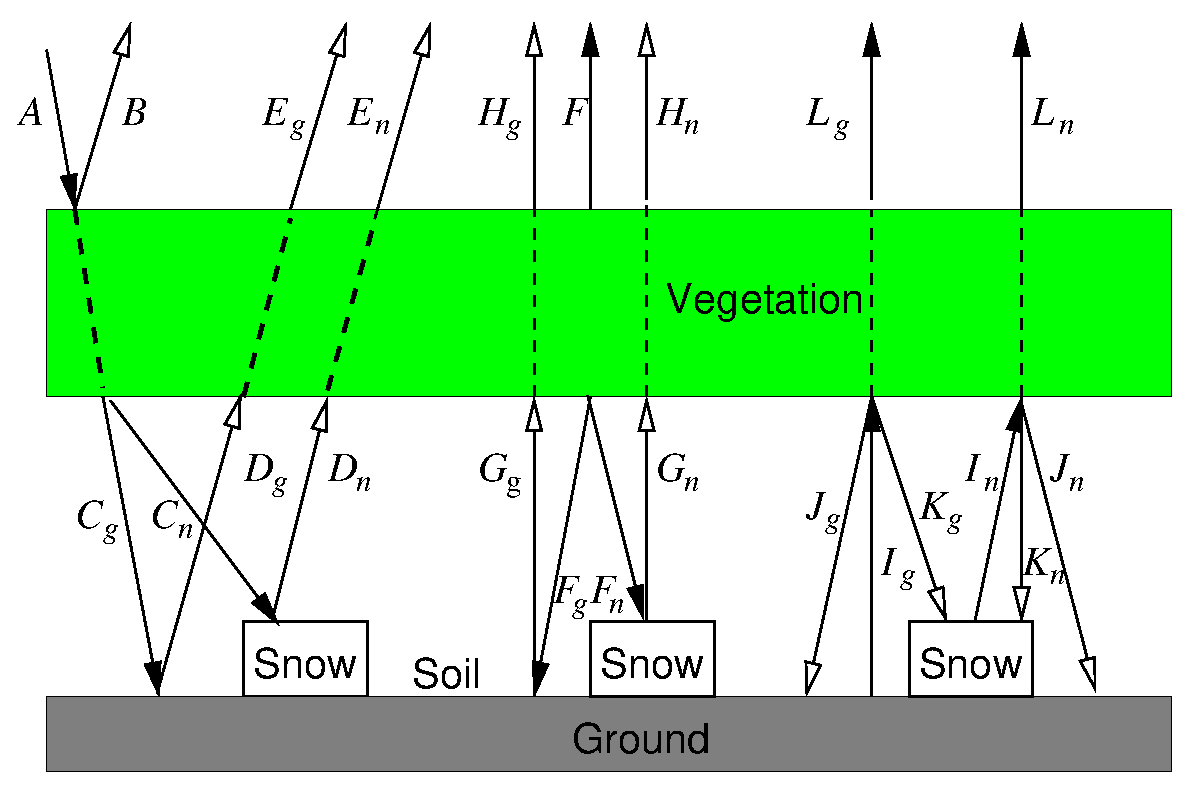
\includegraphics[angle=0, width=12cm, clip=true, trim=0cm 0cm 0cm 0cm]{EPS/lwnet_meb.eps}}
\caption{Simple schematic for longwave radiation transfer for one
reflection and up to three emitting surfaces (in addition to the
down-welling atmospheric flux). Hollow arrows indicate
fluxes after one reflection.}
\label{fig:meb_lwsnow_vg}
\end{figure}
%%%%%%%%%%%%%%%%%%%%%%%%%%%%%%%%%%%%%%



The effective surface radiative temperature (which may be required by the atmospheric radiation
scheme or for comparison with satellite-based data etc.) 
is diagnosed as
%
%%%%%%%%%%%%%%%%%%%%%%%%%
\begin{equation}
  \label{eq:meb_lwup_ts_total_eff}
T_{rad} = {\left[\frac{LW\uparrow - LW\downarrow
      \left(1-{\overline\epsilon}_s\right)}
{{\overline\epsilon}_s \, \sigma}\right]}^{1/4}
%
\end{equation}
%%%%%%%%%%%%%%%%%%%%%%%%%
%
where $\sigma$ is the Stefan-Boltzmann constant, and 
${\overline\epsilon}_s$ represents
the effective surface emissivity. In Eq.~\ref{eq:meb_lwup_ts_total_eff},
there are two knowns ($LW$ fluxes) and two unknowns ($T_{rad}$ and
${\overline\epsilon}_s$). Here we opt to pre-define
${\overline\epsilon}_s$ in a manner which is consistent with the
various surface contributions as
%
%%%%%%%%%%%%%%%%%%%%%%%%%
\begin{equation}
  \label{eq:meb_emis_sfc_eff}
{\overline\epsilon}_s = p_{sng}\,{\overline\epsilon}_{sn} + \left( 1 - p_{sng}\right){\overline\epsilon}_{sg}
%
\end{equation}
%%%%%%%%%%%%%%%%%%%%%%%%%
%
The canopy-absorption weighted 
effective snow and ground emissivities are defined, respecitvely, as
%
%%%%%%%%%%%%%%%%%%%%%%%%%
%\begin{subequations}
\begin{align}
 \label{eq:meb_lw_emis_sfc_terms_n}
{\overline\epsilon}_{sn} = & 
        {\overline\sigma}_{n\,LW}       \,\epsilon_v \,+\, 
\left(1-{\overline\sigma}_{n\,LW}\right)\,\epsilon_n
\\
 \label{eq:meb_lw_emis_sfc_terms_g}
{\overline\epsilon}_{sg} = & 
        {\overline\sigma}_{g\,LW}       \,\epsilon_v \,+\, 
\left(1-{\overline\sigma}_{g\,LW}\right)\,\epsilon_g
%
\end{align}
%\end{subequations}
%%%%%%%%%%%%%%%%%%%%%%%%%
%
where $\epsilon_v$, $\epsilon_g$ and $\epsilon_n$ represent 
the emissivities of the vegetation, snow-free ground and 
the ground-based snowpack, respectively. 
The ground and vegetation emissivities are given by ECOCLIMAP for
spatially distributed simulations, or they can be prescribed for local
scale studies. The snow emissivity is currently defined as $\epsilon_n=0.99$.
%based on the flood-weighted water and soil
%emissivities as
%
%%%%%%%%%%%%%%%%%%%%%%%%%
%\begin{equation}
%  \label{eq:meb_lwup_emis_flood}
%{\overline\epsilon}_g = p_{ff} \epsilon_{ff} + \left(1-p_{ff}\right)\epsilon_g
%
%\end{equation}
%%%%%%%%%%%%%%%%%%%%%%%%%
%
%where $\epsilon_{ff}$ is the emissivity of the flooded area,
%and $\epsilon_g$ is the snow-free flood-free ground emissivity.
%
The effect of longwave absorption through the non-snow buried
part of the vegetation canopy is included as
%
%%%%%%%%%%%%%%%%%%%%%%%%%
%\begin{subequations}
\begin{align}
 \label{eq:meb_lw_sig_emis_sfc_terms_n}
{\overline\sigma}_{n\,LW} = & 
\left[1 \,-\, p_{sng} \,-\, p_{n\alpha}\left(1-p_{sng}\right)\right]
\sigma_{LW} 
\,+\, 
\left[p_{sng} \,+\, p_{n\alpha}\left(1-p_{sng}\right)\right]
\sigma_{f\,LW}
\\
 \label{eq:meb_lw_sig_emis_sfc_terms_g}
{\overline\sigma}_{g\,LW} = & 
\left[1 \,-\, p_{sng}\left(1-p_{n\alpha}\right)\right]
\sigma_{LW} 
\,+\, 
p_{sng}\left(1-p_{n\alpha}\right)
\sigma_{f\,LW}
%
\end{align}
%\end{subequations}
%%%%%%%%%%%%%%%%%%%%%%%%%
%
where the canopy absorption is defined as
%
%%%%%%%%%%%%%%%%
\begin{equation}
\label{eq:meb_sigma_lw}
%
\sigma_{LW} = 1 - {\mathrm{exp}}\left( -\tau_{LW} \, LAI \right) = 1 - \chi_v
%
\end{equation}
%%%%%%%%%%%%%%%%
%
and $\tau_{LW}$ represents a longwave radiation transmission factor which can be species 
(or land classification) dependent, and $\chi_v$ is defined as a
vegetation view factor. 
%
The absorption over the under-story snow-covered fraction of the grid
box is modeled quite simply from Eq.~\ref{eq:meb_sigma_lw} as
%
%%%%%%%%%%%%%%%%
\begin{equation}
\label{eq:meb_sigma_f_lw}
%
\sigma_{f\,LW} \,=\, 
%1 - {\mathrm{exp}}\left[ -\tau_{LW} \, LAI
% \left(1-p_{n\alpha}\right)\right] \,=\, 
1 - {\mathrm{exp}}\left[ -\tau_{LW} \, LAI_n \right]
%
\end{equation}
%%%%%%%%%%%%%%%%
%
so that transmission is unity (no absorption or reflection by the canopy: 
${\overline\sigma}_{LW}=\sigma_{f\,LW}=0$) when $p_{n\alpha}=1$
(i.e. when the canopy has been buried by snow).
%When none of the canopy is buried by the main snowpack then $p_{n\alpha}=0$ so
%that $p_{sng}^\prime=p_{sng}$ which means that
%${\overline\sigma}_{LW}=\sigma_{f\,LW}=\sigma_{LW}$.
$LAI_n$ is used to represent the $LAI$ which has been reduced owing to
burial by the snowpack and is simply defined as:
%
%%%%%%%%%%%%%%%%%%%%%%%%%
\begin{equation}
  \label{eq:meb_lai_snow_modif}
LAI_n = LAI \left(1 \,-\, p_{n\,\alpha}\right)
\end{equation}
%%%%%%%%%%%%%%%%%%%%%%%%%
%
From Eq.s~\ref{eq:meb_emis_sfc_eff}-\ref{eq:meb_lw_sig_emis_sfc_terms_g}, it
can be seen that when there is no snowpack (i.e. $p_{sng}=0$ and
$p_{n\alpha}=0$),
%or flooded fraction ($p_{ff}=0$),
then the effective surface emissivity is simply an absorption-weighted
soil-vegetation value defined as ${\overline\epsilon}_s =  
\sigma_{LW}       \,\epsilon_v \,+\, 
\left(1-\sigma_{LW}\right)\,\epsilon_g$.
%
%See Appendix~\ref{app:meb_lwrad_flux_expressions} for the derivation of
%the net longwave radiation terms in Eq.~\ref{eq:meb_lwup_resid}.


%%%%%%%%%%%%%%%%%%%%%%%%%%%%%%%%%%%%%%%%%%%%%%%%%%%%%%%%%%%%%%%%%%%%%%%%%%%%%%%%%%

%The flooded fraction of the gridbox uses a ground-flooded zone composite
%energy budget, so to consider water surfaces we have defined
%an effective snow-free ground albedo as
%%
%%%%%%%%%%%%%%%%%%%%%%%%%%
%\begin{equation}
%  \label{eq:swup_resid_flood}
%{\overline\alpha}_g = p_{ff} \alpha_{ff} + \left(1-p_{ff}\right)\alpha_g
%%
%\end{equation}
%%%%%%%%%%%%%%%%%%%%%%%%%
%
%where $p_{ff}$ is the sub-grid flooded fraction, $\alpha_{ff}$ is the effective albedo of the flooded area,


The complete expression for the vegetation canopy net longwave radiation 
with an infinite number of reflections can be expressed as a
series expansion 
(e.g. Braud, 2000\nocite{braud_00}) 
as a function of the
temperatures of the emitting surfaces ($T_v$, $T_{g,1}$, 
$T_{n,1}$), their respective emissivities
($\epsilon_v$, $\epsilon_g$ and $\epsilon_n$) and the canopy longwave
absorption function,
$\sigma_{LW}$ (Eq.~\ref{eq:meb_sigma_lw}).
%
The MEB expressions are derived by explicitly expanding
the series 
%This is done to facillitate computing the flux components
%for the different surfaces explicitly (we compare our approximate expressions to
%the series approximations in the next section).
%
%First
and assuming one reflection from each emitting source, which is
a good approximation since emissivities are generally close to unity
(fluxes from a single reflection are proportional to $1-\epsilon_x$ where $x$ represents
$g$, $v$ or $n$, and $\epsilon$ is close
to unity for most natural surfaces).
%Therefore all higher order terms which involve products of reflected fluxes
%are neglected (since such terms will be at least an order of magnitude
%smaller than the terms involing a single reflection).

Snow is considered to be intercepted by the vegetation canopy and to accumulate
on the ground below. 
%The corresponding schematic of the radiative transfer is shown in
%Fig.~\ref{fig:lwsnow_vg}.
%
The canopy-intercepted snow is treated using a composite approach,
so that the canopy temperature, $T_v$, represents the effective temperature of
the canopy-intercepted snow composite. The canopy emissivity is therefore simply defined as
%
%%%%%%%%%%%%%%%%
\begin{equation}
\label{eq:meb_emis_v_n}
%
{\overline\epsilon}_v = \left( 1 - p_{nv}\right) \epsilon_v \,+\, p_{nv}\,\epsilon_{n}
%
\end{equation}
%%%%%%%%%%%%%%%%
%
%where 
%$p_{nv}$ represents the fraction of the canopy covered by intercepted snow, and
%$\epsilon_{n}$ represents the emissivity of the intercepted snow.
%
In order to facilitate the use of a distinct multi-layer snow process
scheme, we
split the fluxes between those interacting with the snowpack and the
snow-free ground.
%
The expressions for the snow-free 
%understory layer 
surface 
are
%
%%%%%%%%%%%%%%%%%%%%%%%%%
\begin{subequations}\label{eq:meb_lw_g_n_terms}
\begin{align}
 \label{eq:meb_lw_g_n_terms_a}
A_{g} = & LW\downarrow \,\left(1-p_{sng}\right)
\\
 \label{eq:meb_lw_g_n_terms_b}
B_{g} = & A_{g}\,\sigma_{LW}\,\left(1-{\overline\epsilon}_v\right)
\\
 \label{eq:meb_lw_g_n_terms_c}
C_{g} = & A_{g}\,\left(1-\sigma_{LW}\right)
\\
 \label{eq:meb_lw_g_n_terms_d}
D_{g} = & C_{g} \,\left(1-\epsilon_g\right)
\\
 \label{eq:meb_lw_g_n_terms_e}
E_{g} = & D_{g}\left(1-\sigma_{LW}^\prime\right)
\\
 \label{eq:meb_lw_g_n_terms_f}
F_{g} = & \sigma_{LW}^\prime\, \sigma \, {\overline\epsilon}_v\, T_v^4\,\left(1-p_{sng}\right)
\\
 \label{eq:meb_lw_g_n_terms_g}
G_{g} = & F_{g}\,\left(1-\epsilon_g\right)
\\
 \label{eq:meb_lw_g_n_terms_h}
H_{g} = & G_{g}\,\left(1-\sigma_{LW}^\prime\right)
\\
 \label{eq:meb_lw_g_n_terms_i}
I_{g} = & \sigma \, \epsilon_g\, T_g^4\,\left(1-p_{sng}\right)
\\
 \label{eq:meb_lw_g_n_terms_j}
J_{g} = & I_{g}\,\sigma_{LW}^\prime\,\left(1-{\overline\epsilon}_v\right) \,\left(1-p_{sng}^\prime\right)
\\
 \label{eq:meb_lw_g_n_terms_k}
K_{g} = & I_{g}\,\sigma_{LW}^\prime\,\left(1-{\overline\epsilon}_v\right) \,p_{sng}^\prime
\\
 \label{eq:meb_lw_g_n_terms_l}
L_{g} = & I_{g}\,\left(1-\sigma_{LW}^\prime\right)
%
\\
 \label{eq:meb_lw_g_n_terms_png}
p_{sng}^\prime = & p_{sng}\left(1-p_{n\alpha}\right)
%
\end{align}
\end{subequations}
%%%%%%%%%%%%%%%%%%%%%%%%%
%
and the equations for the snow-covered under-story fraction are
%
%%%%%%%%%%%%%%%%%%%%%%%%%
\begin{subequations}\label{eq:meb_lw_n_n_terms}
\begin{align}
 \label{eq:meb_lw_n_n_terms_a}
A_{n} = & LW\downarrow \,p_{sng}
\\
 \label{eq:meb_lw_n_n_terms_b}
B_{n} = & A_{n}\,\sigma_{f\,LW}\,\left(1-\epsilon_v\right)
\\
 \label{eq:meb_lw_n_n_terms_c}
C_{n} = & A_{n}\,\left(1-\sigma_{f\,LW}\right)
\\
 \label{eq:meb_lw_n_n_terms_d}
D_{n} = & C_{n} \,\left(1-\epsilon_n\right)
\\
 \label{eq:meb_lw_n_n_terms_e}
E_{n} = & D_{n}\left(1-\sigma_{LW}^\prime\right)
\\
 \label{eq:meb_lw_n_n_terms_f}
F_{n} = & {\overline\sigma}_{f\,LW}\, \sigma \, \epsilon_v\, T_v^4\,p_{sng}
\\
 \label{eq:meb_lw_n_n_terms_g}
G_{n} = & F_{n}\,\left(1-\epsilon_n\right)
\\
 \label{eq:meb_lw_n_n_terms_h}
H_{n} = & G_{n}\,\left(1-\sigma_{LW}^\prime\right)
\\
 \label{eq:meb_lw_n_n_terms_i}
I_{n} = & \sigma \, \epsilon_n\, T_n^4\,p_{sng}
\\
 \label{eq:meb_lw_n_n_terms_j}
J_{n} = & I_{n}\,\sigma_{LW}^\prime\,\left(1-\epsilon_v\right) \,\left(1-p_{sng}^{\prime\prime}\right)
\\
 \label{eq:meb_lw_n_n_terms_k}
K_{n} = & I_{n}\,\sigma_{LW}^\prime\,\left(1-\epsilon_v\right) \, p_{sng}^{\prime\prime}
\\
 \label{eq:meb_lw_n_n_terms_l}
L_{n} = & I_{n}\,\left(1-\sigma_{LW}^\prime\right)
%
\\
 \label{eq:meb_lw_n_n_terms_png}
p_{sng}^{\prime\prime} = & p_{sng} \,+\, p_{n\alpha}\left(1-p_{sng}\right)
%
\end{align}
\end{subequations}
%%%%%%%%%%%%%%%%%%%%%%%%%
%
where the different terms are again
indicated in Fig.~\ref{fig:meb_lwsnow_vg}.
%
In MEB, the ground-based snowpack depth can increase to the point that
it buries the canopy, thus
for both the snow-covered and snow free under-story fractions 
a modified snow fraction is defined as
%
%%%%%%%%%%%%%%%%
\begin{equation}
\label{eq:meb_sigma_lw_avg}
%
\sigma_{LW}^\prime = \left(1-p_{sng}^\prime\right)\sigma_{LW} \,+\,
p_{sng}^\prime \,\sigma_{f\,LW}
%
\end{equation}
%%%%%%%%%%%%%%%%
%
The factor, $\sigma_{f\,LW}$, over the understory snow-covered fraction of the grid
box is modeled quite simply from Eq.~\ref{eq:meb_sigma_f_lw}.
%
%%%%%%%%%%%%%%%%%
%\begin{equation}
%\label{eq:meb_sigma_f_lw}
%%
%\sigma_{f\,LW} = 1 - {\mathrm exp}\left[ -\tau_{LW} \, LAI \left(1-p_{n\alpha}\right)\right]
%%
%\end{equation}
%%%%%%%%%%%%%%%%%
%%
%so that transmission is unity (no absorbtion or reflection by the canopy: 
%$\sigma_{LW}^\prime=\sigma_{f\,LW}=0$) when $p_{n\alpha}=1$
%(i.e. when the canopy has been buried by snow).
%When none of the canopy is buried by the main snowpack then $p_{n\alpha}=0$ so
%that $p_{sng}^\prime=p_{sng}$ which means that $\sigma_{LW}^\prime=\sigma_{f\,LW}=\sigma_{LW}$.
%
%
The inclusion of the snow-buried canopy fraction in
Eq.s~\ref{eq:meb_lw_g_n_terms_png} and \ref{eq:meb_lw_n_n_terms_png}
causes all of the vegetation transmission and below canopy fluxes to vanish as
$p_{sng}$ and $p_{n\alpha}\rightarrow 0$ so that the only longwave
radiative exchanges occur between the atmosphere and the snowpack in
this limit. 




%=========================================================================================================
\subsubsection{Heat Conduction fluxes}
\label{sec:meb_energy_budget_cond}
%=========================================================================================================

%The sub-surface snow and ground heat conduction fluxes are modeled 
%using Fourier's Law ($G=\lambda\partial T/\partial z$). 
The heat
conduction fluxes in Eq.s~\ref{eq:meb_cgdtgdt_three}-\ref{eq:meb_cndtndt_three}
are modeled 
using Fourier's Law ($G=\lambda\partial T/\partial z$)
and have been defined in previous sections (since MEB uses
either the multilayer diffusive or 2 to 3 layer Force-Restore 
hydrology/soil configurations, coupled to the explicit multilayer snow
scheme ES).
%
The main potential difference between ISBA and ISBA-MEB is that
the heat capacity and thermal conductivity for the ground 
depend either on the thermal properties of the soil
(possibly including organic content)
or on the thermal
properties of the forest litter
in the uppermost layer (Napoly et al., 2017)\nocite{napoly_ea_2017}: 
this parameterization
is described in more detail in Section~\ref{sec:meb_litter}.
%The snow thermal property parameterization is described in \citet{Decharme16}.

%=========================================================================================================
\subsubsection{Aerodynamic Resistances}
\label{sec:meb_resistances} 
%=========================================================================================================

The resistances between the surface and the overlying atmosphere, $R_{a\,n-a}$
and $R_{a\,c-a}$, are based on the values of $C_H$ 
computed from Eq.~\ref{eq:isba_heat_transfer_coef}
between
the overyling atmosphere and the snow surface, and between
the overyling atmosphere and the canopy air space, respectively, where
$C_{Hx}={\left(V_a R_{a\,x-a}\right)}^{-1}$.

%\citet{louis_79}
%modified by \citet{mascart_ea_95} to account for different roughness 
%length values for heat and momentum as in ISBA.
%: the full expressions are given 
%in \citet{noilhan_mahfouf_96}.

%\subsubsection{Aerodynamic Resistance between the bulk vegetation
%layer and the canopy air}

The aerodynamic resistance between the vegetation canopy and the
surrounding airspace can be defined as
%
%%%%%%%%%%%%%%%%%%%%%%%%%
\begin{equation}
  \label{eq:meb_bulk_canopy_resis}
  R_{a\,vg-c} = {\left( g_{av} \,+\, g_{av}^\ast \right)}^{-1}
\end{equation}
%%%%%%%%%%%%%%%%%%%%%%%%%
%
The parameterization of the bulk canopy aerodynamic conductance, $g_{av}$, 
between the canopy and the canopy air is based on 
Choudhury and Monteith (1988)\nocite{Choudhury88}.
It is defined as
%
%%%%%%%%%%%%%%%%%%%%%%%%%
\begin{equation}
  \label{eq:meb_condrb}
  g_{av} = 
%{\Bigg\lbrace
\frac{2 \, LAI \, a_{av}}{\phi_v^\prime}\left(\frac{u_{hv}}{lw}\right)^{1/2}[1-\exp(-\phi_v^\prime/2)].
%\Bigg\rbrace}^{-1}
\end{equation}
%%%%%%%%%%%%%%%%%%%%%%%%%
%
where 
%the resistance in Eq.~\ref{eq:meb_bulk_canopy_resis} is simply
%$R_{av}=g_{av}^{-1}$.
$u_{hv}$ represents the wind speed at the top of the canopy
(m s$^{-1}$),
$LAI$ is the leaf area index (m$^{2}$ m$^{-2}$), and the remaining parameters are
defined in Table~\ref{independent}.
%
The conductance accounting for the free convection correction
from Sellers et al. (1986)\nocite{Sellers86}
is expressed as
%
%%%%%%%%%%%%%%%%%%%%%%%%%
\begin{equation}
  \label{eq:meb_freeconv}
  g_{av}^\ast = \left[ \frac{LAI}{890} \left(\frac{T_{v} -
        T_{c}}{lw}\right)^{1/4}\right]
\hskip1.in \left( T_{v} \geq T_{c} \right)
\end{equation}
%%%%%%%%%%%%%%%%%%%%%%%%%
%
Note that this correction is only used for unstable conditions.
%
The effect of snow burying the vegetation impacts the aerodynamic
resistance of the canopy is simply modeled by modifying the $LAI$
to obtain $LAI_n$ using Eq.~\ref{eq:meb_lai_snow_modif}.
%
The $LAI_n$ is used in
Eq.~\ref{eq:meb_bulk_canopy_resis} to compute $R_{a\,vn-c}$, and this
resistance is limited to 5000 s m$^{-1}$ as $LAI_n \rightarrow 0$.


%\subsubsection{Aerodynamic Resistance between the ground and the canopy air}

%%%%%%%%%%%%%%%%%%%%%%%%%%%%%%%%%%%%%%%%%%%%%%%%%%%%%%%%%%%%%%%%%%%%%%%%%%%%%

The resistance between the ground and the canopy air space is defined as
%
%%%%%%%%%%%%%%%%%%%%%%%%%
\begin{equation}
  \label{eq:meb_resistance_stabcor}
R_{ag-c} = R_{ag\,n}/\psi_H
%
\end{equation}
%%%%%%%%%%%%%%%%%%%%%%%%%
%
where $R_{ag\,n}$ is the default resistance value for neutral conditions. 
%(from Eq.~\ref{eq:meb_rd}).
The stability correction term, $\psi_H$, depends on the canopy
structural parameters, wind speed and temperature gradient
between the surface and the canopy air.
%
The aerodynamic resistance is also based on
Choudhury and Monteith (1988)\nocite{Choudhury88}.
It is assumed that the eddy diffusivity, $K$ (m$^2$ s$^{-1}$), 
in the vegetation layer
follows an exponential profile:
%
%%%%%%%%%%%%%%%%%%%%%%%%%
\begin{equation}
  \label{eq:meb_k_prof}
K\left(z\right) = K\left(z_{hv}\right) \,
\exp\left[\phi_v \left(1-{\frac{z}{z_{hv}}}\right)\right] 
\end{equation}
%%%%%%%%%%%%%%%%%%%%%%%%%
%
where $z_{hv}$ represents the canopy height.
Integrating the reciprocal of the diffusivity defined
in Eq.~\ref{eq:meb_k_prof} from $z_{0g}$ to $d + z_{0v}$ yields
%
%%%%%%%%%%%%%%%%%%%%%%%%%
\begin{equation}
  \label{eq:meb_rd}
  R_{ag\,n} = \frac{z_{hv}}{\phi_v \, K\left(z_{hv}\right)}
\Bigg\lbrace
\exp\left[\phi_v \left(1-{\frac{z_{0g}}{z_{hv}}}\right)\right] \,-\, 
\exp\left[\phi_v \left(1-{\frac{d +
             z_{0v}}{z_{hv}}} \right)\right] 
\Bigg\rbrace
\end{equation}
%%%%%%%%%%%%%%%%%%%%%%%%%
%
The diffusivity at the canopy top is defined as
%
%%%%%%%%%%%%%%%%%%%%%%%%%
\begin{equation}
  \label{eq:meb_Kh}
  K\left(z_{hv}\right) = k \, u_{\ast hv} \, \left(z_{hv} - d\right) 
%= 
%{\frac{k^2 \, u_{hv} \, \left(z_{hv} - d\right)} 
%{{\mathrm{ln}} \left[ \left(z_{hv} - d\right)/z_{0v}\right] }}
\end{equation}
%%%%%%%%%%%%%%%%%%%%%%%%%
%
The von Karman constant, $k$, has a value of 0.4.
The displacement height is defined as 
(Choudhury and Monteith, 1988)\nocite{Choudhury88}
%
%%%%%%%%%%%%%%%%%%%%%%%%%
\begin{equation}
  \label{eq:meb_disph}
  d = 1.1 \, z_{hv} \, {\mathrm{ln}}\left[1 + {\left(c_d \, LAI_f\right)}^{1/4}\right]
\end{equation}
%%%%%%%%%%%%%%%%%%%%%%%%%
%
where
the leaf drag coefficient, $c_d$, is defined from 
Sellers et al. (1996)\nocite{Sellers96}:
%
%%%%%%%%%%%%%%%%%%%%%%%%%
\begin{equation}
  \label{eq:meb_cd}
  c_d = 1.328 \, \left[\frac{2}{{R_e}^{1/2}}\right] + 
0.45 \left[ \frac{1}{\pi}(1-\chi_L) \right]^{1.6}
\end{equation}
%%%%%%%%%%%%%%%%%%%%%%%%%
%
$\chi_L$ represents the Ross-Goudriaan leaf angle distribution function, which has
been estimated according to 
Monteith (1975)\nocite{Monteith75}
(see Table~\ref{meb_independent}), and
$R_e$ is the Reynolds number defined as
%
%%%%%%%%%%%%%%%%%%%%%%%%%
\begin{equation}
  \label{eq:meb_Re}
  {R_e} = \frac{u_l \, lw}{\upsilon}.
\end{equation}
%%%%%%%%%%%%%%%%%%%%%%%%%
%
%The unstable transfer correction for $r_{ag}=r_{ag}/\psi_H$ according to \cite{Sellers86},
%where
%
%%%%%%%%%%%%%%%%%%%%%%%%%
%\begin{equation}
%  \label{eq:meb_phih}
%  \psi_H = \left[ 1 + 9 \frac{T_{g} - T_{c}}{T_{g} u_{hv}^2} z_{hv} \right]^{1/2}.
%\end{equation}
%%%%%%%%%%%%%%%%%%%%%%%%%
%

The friction velocity at the top of the vegetation canopy is
defined as
%
%%%%%%%%%%%%%%%%%%%%%%%%%
\begin{equation}
  \label{eq:meb_ustar_cantop}
u_{\ast hv} = {\frac{k \, u_{hv}}
{{\mathrm{ln}}\left[
\left( z_{hv} - d \right)/z_{0v}\right]}}
\end{equation}
%%%%%%%%%%%%%%%%%%%%%%%%%
%
where the wind speed at the top of the canopy is
%
%%%%%%%%%%%%%%%%%%%%%%%%%
\begin{equation}
  \label{eq:meb_u_cantop}
u_{hv} = f_{hv} \, V_a
\end{equation}
%%%%%%%%%%%%%%%%%%%%%%%%%
%
and $V_a$ represents the wind speed at the reference height, $z_a$,
above the canopy. 
%
The canopy height is defined based on vegetation
class and climate within ECOCLIMAP as a primary parameter. It can
also be defined using an external dataset, such as from a satellite-derived product (as a function of space and time). The vegetation
roughness length for momentum is then computed as a secondary
parameter as a function of the vegetation canopy height.
%
The factor $f_{hv}$ ($\leq 1$) is a stability dependent adjustment factor
%(see Appendix~\ref{app:f_stab_factor}).
%The expressions for the stability factor $f_{hv}$ (Eq.~\ref{eq:u_cantop}) which is used 
%to compute the wind at the top of the vegetation canopy, $u_{hv}$, are 
taken from the RCA LSM 
(Samuelsson et al., 2006; Samuelsson et al., 2011)\nocite{Samuelsson06,Samuelsson11}.
They are defined as
%
%%%%%%%%%%%%%%%%%%%%%%%%%%%%%%
\[ f_{hv} = \left\{ \begin{array}{ll}
        \left( C_{v,N} \,+\, C_{v,S}\right) \sqrt{C_D} \, /k
& \mbox{if $R_i > 0 $}
\\
        \left( C_{v,N} \,+\, C_{v,U}\right) \sqrt{C_D} \, /k
& \mbox{if $R_i \leq 0$}
\end{array} 
\right. \] 
%%%%%%%%%%%%%%%%%%%%%%%%%%%%%%
%%%%%%%%%%%%%%%%%%%%%%%%%
%\begin{subequations}
%\begin{align}
%
%\label{eq:meb_fv_velc_stable} 
%f_{hv} =& \left( C_{v,N} \,+\, C_{v,S}\right) \sqrt{C_D} \, /k
%\hskip.5in
%\left(R_i > 0 \right)
%\\
%%
%\label{eq:meb_fv_velc_unstable} 
%    =& \left( C_{v,N} \,+\, C_{v,U}\right) \sqrt{C_D} \, /k
%\hskip.5in
%\left(R_i \leq 0 \right)
%%
%\end{align}
%\end{subequations}
%%%%%%%%%%%%%%%%%%%%%%%%%
%
where the Richardson number, $R_i$, is defined 
in Eq.~\ref{eq:meb_canopy_ground_rich}.
The coefficients are defined as
%
%%%%%%%%%%%%%%%%%%%%%%%%%
\begin{align}
%
\label{eq:meb_fv_velc_neutral_c} 
C_{v,N} =& {\mathrm{ln}} \Bigg\lbrace 
1 \,+\, \phi_z
\left[\exp \left({\frac{k}{\sqrt{C_{DN}}}}\right) - 1\right]
\Bigg\rbrace 
\\
%
\label{eq:meb_fv_velc_stable_c} 
C_{v,S} =& -
\phi_z
\left(
{\frac{k}{\sqrt{C_{DN}}}}-{\frac{k}{\sqrt{C_{D}}}}
\right)
\\
%
\label{eq:meb_fv_velc_unstable_c} 
C_{v,U} =& -{\mathrm{ln}} \Bigg\lbrace 
1 \,+\, \phi_z
\left[\exp \left(
{\frac{k}{\sqrt{C_{DN}}}}-{\frac{k}{\sqrt{C_{D}}}}
\right) 
- 1\right]
\Bigg\rbrace 
%
\end{align}
%%%%%%%%%%%%%%%%%%%%%%%%%
%
where the drag coefficient, $C_D$, and the drag coefficient for
neutral conditions, $C_{DN}$, are computed between the
canopy air space 
%(at height $z_c$)
and the free atmosphere above using the standard ISBA
surface layer
transfer functions (Eq.~\ref{eq:isba_drag_transfer_coef} and
Eq.~\ref{eq:isba_drag_transfer_coef_neutral}, respectively).
%\citep{noilhan_mahfouf_96}.




The dimensionless height scaling factor
is defined as 
%
%%%%%%%%%%%%%%%%%%%%%%%%%
\begin{equation}
%
\label{eq:meb_z_ratio_measure} 
\phi_z = {\frac{\left(z_{hv}-d\right)}{z_r}}
\hskip1.in
\left( \phi_z\leq 1 \right)
\end{equation}
%%%%%%%%%%%%%%%%%%%%%%%%%
%
The reference height is defined as $z_r=z_a-d$
for simulations where the reference height is sufficiently above
the top of the vegetation canopy. This is usually the case for local
scale studies using observation data.
When MEB is coupled to an atmospheric model, however, the lowest model
level can be below the canopy height, so for coupled model
simulations
$z_r = {\mathrm{max}}\left(z_a,\,z_{hv}-d+z_{min}\right)$
where $z_{min}=2$ (m).


%\subsubsection{Stability Correction}

Finally, the stability correction 
factor from Eq.~\ref{eq:meb_resistance_stabcor} is defined
as
%
%%%%%%%%%%%%%%%%%%%%%%%%%
\begin{subequations}
\begin{align}
  \label{eq:meb_unstable_cor_rich}
\psi_H & = {\left( 1 \,-\, a_{hv}\,R_i\right)}^{1/2}
\hskip2.3in \left( R_i \leq 0 \right)
\\
%
%\label{eq:meb_stable_cor_rich}
%
%\psi_H & = {\left( 1 \,-\, a_{hv}\,R_i\right)}^{1/2}
%\hskip2.3in \left( R_i \leq 0\right)
%\\
%
%\label{eq:meb_unstable_cor_rich_new}
%\psi_H &= {\left( 1 \,-\, a_{hv}\,R_i\right)}^{1/2} 
%\hskip2.5in \left( R_i \leq 0 \right)
%\\
\label{eq:meb_stable_cor_rich_new_trans}
& = 
%
%OLD%{\left[ 1 \,+\, b\, \left({\frac{R_i}{R_{i,crit}}}\right)\right]}^{-2} \,\,=\,\,
%OLD%{\left( 1 \,+\, b_{hv}\,R_i\right)}^{-2}
%OLD%\hskip.5in \left( R_i > 0 \right)
%
{\frac{1}{1 + b\, R_i {\left(1+c\,R_i\right)}^{1/2}}}
\left[{ 1 \,+\, \left({\frac{R_i}{R_{i,crit}}} \right) \left(f_{z0} - 1 \right)}\right]
\hskip.25in \left( R_i > 0 \,\,{\mathrm{and}}\,\, R_i \leq R_{i,crit} \right)
\\
\label{eq:meb_stable_cor_rich_new}
& = 
%
{\frac{f_{z0}}{1 + b\, R_i {\left(1+c\,R_i\right)}^{1/2}}} 
\hskip2.in \left( R_i > R_{i,crit}\right)
%
\end{align}
\end{subequations}
%%%%%%%%%%%%%%%%%%%%%%%%%
%
where the Richardson number is defined as
%
%%%%%%%%%%%%%%%%%%%%%%%%%
\begin{equation}
  \label{eq:meb_canopy_ground_rich}
R_i = {\frac { -g\,z_{hv}\,\left(T_s - T_c \right)}{T_s \, {u_{hv}}^2}}
%
\end{equation}
%%%%%%%%%%%%%%%%%%%%%%%%%
%
Note that strictly speaking, the temperature factor in the denominator should be defined as
$\left(T_s+T_c\right)/2$, but this has only a minor impact for our
purposes.
%
The so-called critical Richardson number, $R_{i,crit}$, is set to 0.2.
This parameter has been defined assuming that
some turbulent exchange is likely always present (even if intermittent), 
but it is recognized 
that eventually a more robust approach should be developed for very
stable surface layers. 
%(e.g. )\nocite{galperin2007}.
%
The expression for unstable conditions
(Eq.~\ref{eq:meb_unstable_cor_rich}) 
is from 
Sellers et al. (1996)\nocite{Sellers96} 
where
the structural parameter is defined as $a_{hv}=9$. 
%
%Eq.~\ref{eq:meb_unstable_cor_rich} was likely developed with unstable conditions in mind, and it also
%works for slightly stable conditions. But note that one can readily see from
%Eq.~\ref{eq:meb_unstable_cor_rich} that $R_i$ is constrained to be $\leq
%1/{a_{hv}}$, so that a threshold value of either $\phi_H$ or $R_i$ must
%be prescribed for stable conditions.
%a square root of a negative number. 
%So, a somewhat arbitrary threshold must be defined to prevent this.
%In MEB, it was initially decided to define a critical Richardson number as 
%
%%%%%%%%%%%%%%%%%%%%%%%%%%
%\begin{equation}
%  \label{eq:meb_rich_crit_gc}
%R_{ic} = \left[ 1 \, - \, \left({\frac {1}{R_{acf}}}\right) \right]{\frac {1}{a_{hv}}}
%%
%\end{equation}
%%%%%%%%%%%%%%%%%%%%%%%%%%
%
%where the value enclosed in brackets is less than unity. In studies done by C. Canac et al., a 
%value of $R_{acf}=200$ was used, therefore $R_{ic}\approx 0.11$. 
%
%In fact, the stable parameterization becomes quite important
%For the case of snowpack underlying the canopy, very stable
%conditions can develop, especially during spring snow melt, so that the
%model can become quite sensitive to the form of $\phi_H$.
%aabtmptest
%First, simply from a theoretical standpoint, $R_{ic}=0.11$ is significantly larger than the usual limit value of 0.20
%(and for snowpack, such large Richardson numbers can be commonplace).
%Second, small changes
%For example, if Eq.~\ref{eq:meb_unstable_cor_rich} is used for stable
%conditions, 
%relatively small changes 
%in $R_i$ can result in large changes in $\psi_H$, which is counter to what is usually done for stable conditions
%(generally, $\psi_H \rightarrow 0$ gradually/asymptotically as $R_i\rightarrow \infty$). 
%Finally, usually there is a point of inflection
%in the curve describing $\psi_H$ at $R_i=0$, so that there is a exponential-type drop off in turbulent
%exchange for $R_i >0$. If this is not the case, large
%turbulent exchange can occur during snow melt conditions, resulting in
%large negative heat fluxes and excessive melt rates.

%%%%%%%%%%%%%%%%%%%%%%%%%%%%%%%%%%%%%%
\begin{figure}[!b]
\centerline{
%\includegraphics[angle=270, width=11cm, clip=true, trim=0cm 0cm 0cm 0cm]{FIGURES/psi_H_z0-z0h.eps}}
\includegraphics[angle=270, width=14cm, clip=true, trim=0cm 0cm 0cm 0cm]{EPS/psi_H_z0-z0h.ps}}
\caption{Stability correction term is shown using the Sellers formulation 
  for $R_i \leq 0$ while the function for stable conditions adapted
  from ISBA ($R_i > 0$) for two ratios of $z_{0g}/z_{0gh}$. The ground surface roughness length is
  defined in Table~\ref{meb_independent}.}
\label{fig:stab_cor_gc}
\end{figure}
%%%%%%%%%%%%%%%%%%%%%%%%%%%%%%%%%%%%%%

%\subsection{New stable formulation}
%
It is generally accepted 
that there is a need to improve the parameterization of the exchange
coefficient for
extremely stable conditions typically encountered over snow
(e.g.s Niu and Yang, 2004; Andreadis et al., 2009)
\nocite{niu_yang_2004,andreadis_ea_2009}.
%
Since the goal here is not to develop a new parameterization,
we simply modify the expression for stable conditions
by using the standard function from ISBA. 
The standard ISBA stability correction for stable conditions is given
by Eq.~\ref{eq:meb_stable_cor_rich_new}
where $b=15$ and $c=5$.
%\citep{noilhan_mahfouf_96}.
The factor which takes into account differing roughness lengths for heat and momentum
is defined as
%
%%%%%%%%%%%%%%%%%%%%%%%%%
\begin{equation}
  \label{eq:meb_stable_cor_rich_orig_isba}
f_{z0} = 
%\left[{ 
{\frac{ {\mathrm{ln}}\left(z_{hv}/z_{0g}   \right) }
      { {\mathrm{ln}}\left(z_{hv}/z_{0gh}\right) } }
%}\right]
%
\end{equation}
%%%%%%%%%%%%%%%%%%%%%%%%%
%
where $z_{0gh}$ is the ground roughness length for scalars.
%, and the reference height, $z$, is set to $z_{hv}$.
The weighting function (i.e. ratio of $R_i$ to $R_{i,crit}$) in Eq.~\ref{eq:meb_stable_cor_rich_new_trans} 
is used in order to avoid a discontinuity at $R_i=0$ (the roughness length factor effect vanishes at $R_i=0$)
in Eq.~\ref{eq:meb_stable_cor_rich_new}.
%Eq.~\ref{eq:meb_stable_cor_rich_new} is identical to that
%proposed 
%by \citet{noilhan_mahfouf_96} for stable conditions.
%
%
An example of Eq.~\ref{eq:meb_stable_cor_rich_new} 
is shown in Fig.~\ref{fig:stab_cor_gc} using the $z_{0g}$ from
Table~\ref{independent}, 
%vegetation heights, $z_{hv}$, of 5 and 10 m,
and for $z_{0gh}/z_{0g}$ of 0.1 and 1.0.
%
Finally, the resistance between the ground-based snowpack, $R_{a\,n-c}$, and the canopy air
use the same expressions as for the aerodynamic resistance between the
ground and the canopy air outlined herein, but with the surface
properties of the snowpack (namely the roughness length and snow surface temperature).
%Note that as the vegetation becomes buried (i.e. $p_{n\,alpha}>0$), 


%%%%%%%%%%%%%%%%%%%%%%%%%%%%%%
\begin{table}[h]
\caption{Surface vegetation canopy turbulence parameters which are constant.}
\begin{center}
\begin{footnotesize}
\begin{tabular}{clllll}
\hline
Symbol		& Definition			& Unit		& Value	& Reference		& Comment \\
\hline
\hline
%$g$		& Acceleration of gravity	& m s$^{-2}$	& 9.81	\\
%$G_2$		& Adjustment factor		& -		& 0.75	& \nocite{Xue91}	& Eq. 13 \\
%$k$		& von Karman constant		& -		& 0.4 \\
$a_{av}$		& canopy conductance scale factor & m
s$^{-1/2}$	& 0.01	& 
Choudhury and Monteith (1988)\nocite{Choudhury88}	& Eq. 26 \\
$\phi_v^\prime$	& attenuation coeff. for wind	& -		& 3
& 
Choudhury and Monteith (1988)\nocite{Choudhury88} & p 386 \\
$lw$		& leaf width			& m		& 0.02	\\
$\phi_v$	& attenuation coeff. for mom.	& -		& 2
& 
Choudhury and Monteith (1988)\nocite{Choudhury88} & p 386 \\
$z_{0g}$		& roughness of soil surface	& m		& 0.007	\\
$\chi_L$	& Ross-Goudriaan leaf angle dist. & -		& 0.12
& 
Monteith (1975)\nocite{Monteith75}	& p 26 \\
$u_l$		& Typical local wind speed	& m s$^{-1}$	& 1
& Sellers et al. (1996)\nocite {Sellers96}	& Eq. B7 \\
$\upsilon$	& Kinematic viscos. of air	& m$^2$ s$^{-1}$ & $0.15\times10^{-4}$ \\

\hline
\end{tabular}
\end{footnotesize}
\end{center}
\label{meb_independent}
\end{table}
%%%%%%%%%%%%%%%%%%%%%%%%%%%%%%%%%%%%




%=========================================================================================================
\subsubsection{Ground resistance}
%=========================================================================================================

The soil resistance term is
defined based on 
Sellers et al. (1992)\nocite{sellers_ea_1992} 
as
%
%%%%%%%%%%%%%%%%%%%%%%%%%%
\begin{equation}
\label{eq:meb_resis_grnd}
R_g = {\mathrm{exp}}\left[a_{Rg} - b_{Rg} \,
\left({\overline w_g}/{\overline w_{sat}}\right)\right] \,\,\,.
%
\end{equation}
%%%%%%%%%%%%%%%%%%%%%%%%%%
%
The coefficients are $a_{Rg}=8.206$ and $b_{Rg}=4.255$, and the
vertically averaged volumetric water content and saturated volumetric water content 
are given by ${\overline w_g}$ and ${\overline w_{sat}}$,
respectively. The averaging is done from one to several upper layers.
%
Indeed, the inclusion of an explicit ground surface energy budget
makes it more conceptually straightforward to include a ground
resistance compared to the original composite soil-vegetation
surface.
%, and many models use such a resistance term together with the
%humidity function as it has been shown to both generally improve
%results and it has numerical advantages compared to using the
%so-called alpha parameterization alone 
%
The ground resistance is often used as a surrogate for an additional
resistance arising due to a forest litter layer, therefore
the soil resistance is set to zero 
when the litter layer option is activated. 
Finally, the coefficients $a_{Rg}$ and $b_{Rg}$ were determined from a case study for a
specific location, and could possibly be location dependent. But
currently these values are used, in part, since the
litter formulation is the default
configuration for MEB for forests as it generally gives better surface
fluxes 
(Napoly et al., 2017)\nocite{napoly_ea_2017}.


%----------------------------------------------------------------------------------------



%----------------------------------------------------------------------------------------




%=========================================================================================================
\subsubsection{Water Budget}
\label{sec:meb_water_budget}
%=========================================================================================================

The governing equations for (water) mass for the bulk canopy, and
surface snow and ground layers are written as
%
%%%%%%%%%%%%%%%%%%%%%%%%%
\begin{align}
%
\label{eq:meb_dwrvdt}
{\frac {\partial W_{r}}{\partial t}} = & 
 P_{rv} \,+\, {\mathrm{max}}\left(0, \, -E_{tr}\right) 
- E_{r} \,-\, D_{rv} \,-\, \Phi_{v}
\\
%
\label{eq:meb_dtwrnvdt}
{\frac {\partial W_{r\,n}}{\partial t}} = & 
I_{n} \,-\, U_{n} \,-\, E_{rn} \,+\, \Phi_{v}
%\,+\,  E_{n,v cor} &
%
\\
%
\label{eq:meb_dtwndt}
%p_{sng} \, {\frac {\partial W_{n,1}}{\partial t}} = & P_s \,-\, 
%I_{n} \,+\, U_{n} + 
%\nonumber\\
%& p_{sng} \, \left(
%P_r \,-\, P_{rv} \,+\, D_{rv}
%- F_{nl,1} - E_n
%- \Phi_{n,1}
%+ \xi_{nl,1} 
%\right)
%\\
%
p_{sng} \, {\frac {\partial W_{n,1}}{\partial t}} = & P_s \,-\, 
I_{n} \,+\, U_{n} + 
p_{sng} \, \left(
P_r \,-\, P_{rv} \,+\, D_{rv}
- F_{nl,1} - E_n
+ \Phi_{n,1}
+ \xi_{nl,1} 
\right)
\\
%
\label{eq:meb_dtwgdt} 
\rho_w \, \Delta z_{g,1} {\frac {\partial w_{g,1}}{\partial t}} = & 
\left( P_r \,-\, P_{rv} \,+\, D_{rv} \,-\, E_g\right)
\left(1 - p_{sng}\right) 
+ p_{sng}\,F_{nl,N_n} 
\,-\, R_0 - F_{g,1} - \Phi_{g,1} 
%- {\cal F}_{2,k}\, {\mathrm max}\left(0, \, E_{tr}\right) 
\\
%
\label{eq:meb_dtwgfdt}
\rho_w \, \Delta z_{g,1} {\frac {\partial w_{gf,1}}{\partial t}} = &
\Phi_{g,1} - E_{gf}\,\left(1 - p_{sng}\right)   
%
\end{align}
%%%%%%%%%%%%%%%%%%%%%%%%%
%
where $W_{r}$
%, $W_{r\,gv}$ 
and $W_{r\,n}$ represent the vegetation
canopy water stores: intercepted water, 
%the understory vegetation
%intercepted water,
and the intercepted snow and frozen water (all in kg m$^{-2}$), respectively.
$W_{n,1}$ represents the snow liquid water equivalent (SWE) for the
uppermost
snow layer of the multi-layer scheme.
The soil liquid water and equivalent frozen water equivalent
volumetric water
content are defined as $w_g$ and $w_{gf}$, respectively (m$^3$
m$^{-3}$). 

%%%

The interception reservoir, $W_r$, is modeled as single
layer bucket, with losses represented by evaporation, $E_r$, and
canopy drip, $D_{rv}$,  of liquid water which exceeds a maximum holding capacity
(see Sect.~\ref{sec:meb_rain_interception} for details). 
Sources include condensation (negative $E_r$ and $E_{tr}$) and
$P_{rv}$ which represents the intercepted precipitation. 
The positive part of $E_{tr}$ is extracted from the sub-surface soil
layers as a function of soil moisture and 
a prescribed vertical root zone distribution.
%\citep{Decharme16}.
%
This equation is the same as that used in ISBA, except for the
addition of the phase change term, $\Phi_{v}$ (kg m$^{-2}$
s$^{-1}$). This term has been introduced owing to the introduction of
an explicit canopy snow interception reservoir, $W_{r\,n}$: the
canopy snow and 
liquid water reservoirs can exchange mass via this term which
is modeled as melt less
freezing. 
%
The remaining
rainfall ($P_r-P_{rv}$) is partitioned between the snow-free and
snow-covered ground surface,
where $P_r$ represents the total grid-cell rainfall rate.
The canopy snow interception is more complex, and represents certain
baseline processes such as snow interception, $I_n$, and unloading,
$U_n$: see Sect.~\ref{sec:meb_snow_interception} for details. 
%The latent heat of fusion is represented by $L_m$.

The soil water and snow liquid water vertical fluxes at the base of
the surface ground and snow are represented,
respectively,
by $F_{g,1}$ using Darcy's Law and by $F_{nl,1}$ using a
tipping-bucket scheme (kg m$^{-2}$ s$^{-1}$). 
The liquid water flux at the base of the snowpack, $F_{nl,N_n}$, is
directed downward into the soil and consists in the liquid water in
excess of the lowest model liquid water holding capacity.
%Finally, $R_0$ represents the surface runoff which is modeled using a sub-grid
%parameteruzation for spatially distributed applications, or simply
%excess saturation when the model is used at the local scale.
%
A description of the
explicit snow and soil schemes are given in 
Sections~\ref{sec:isba_multi_layer_snow} 
and \ref{sec:isba_diffusion_soil}, respectively.
%\citep{boone_etchevers_01} 
%and \citep{Decharme_ea11}, respectively.
%
%The upper boundary condition (infiltration) is defined as
%
%%%%%%%%%%%%%%%%%%%%%%%%%
%\begin{equation}
%%
%\label{eq:meb_grnd_sfc_liq_wat_flux}
%
%F_{g,0} = \left( P_r \,-\, P_{rv} \,+\, D_{rv} \right)\left(1 -
%  p_{sng}\right) \,-\, R_0
%
%\end{equation}
%%%%%%%%%%%%%%%%%%%%%%%%%
%
$R_0$ is the so-called surface runoff. It accounts for sub-grid
heterogeneity of precipitation, soil moisture and for when 
potential infiltration exceeds a maximum
rate: see Sections~\ref{sec:isba_runoff_var_precip} and \ref{sec:isba_runoff}.
%\nocite{Decharme_ea06}.
%
The soil liquid water equivalent ice content can have some losses
owing to sublimation in the uppermost soil layer, $E_{gf}$, but it mainly
evolves owing to phase changes from soil water freeze-thaw, $\Phi_{g}$.
%
%The snow liquid water equivalent (SWE) in each snow layer is
%represented by $W_n$ (kg m$^{-2}$).
%In Eq.~\ref{eq:meb_dtwndt}, the liquid water fluxes across the layer
%interfaces are defined as $F_{nl}$. 
%The upper boundary condition (at the snowpack surface)
%is the surface liquid water infiltration 
%defined as
%
%%%%%%%%%%%%%%%%%%%%%%%%%
%\begin{equation}
%
%\label{eq:meb_snow_sfc_liq_wat_flux}
%
%F_{nl,0} = P_r \,-\, P_{rv} \,+\, D_{rv} 
%
%\end{equation}
%%%%%%%%%%%%%%%%%%%%%%%%%
%
%
The remaining symbols in Eq.s~\ref{eq:meb_dwrvdt}-\ref{eq:meb_dtwrnvdt}
are defined and described in Sections~\ref{sec:meb_rain_interception} and
~\ref{sec:meb_snow_interception}.


%=========================================================================================================
\subsubsection{Snow Interception within the canopy}
\label{sec:meb_snow_interception}
%=========================================================================================================

The intercepted snow mass budget is described by
Eq.~\ref{eq:meb_dtwrnvdt}, while the energy budget is included as a part
of the bulk canopy prognostic equation (Eq.~\ref{eq:meb_cvdtvdt_three}).
The positive mass contributions acting to increase intercepted snow on
canopy are snowfall interception, $I_{n}$, water on canopy that freezes, $\Phi_{v}<0$, and sublimation of
water vapor to ice, $E_{rn}<0$. 
Unloading, $U_{n}$, sublimation, $E_{rn}>0$, and snow melt, $\Phi_{v}>0$, are the sinks. 
All of the terms are in kg m$^{-2}$ s$^{-1}$.
%
It is assumed that intercepted rain and snow can co-exist on the canopy. 
%
The intercepted
snow is assumed to
have the same temperature as the canopy, $T_v$, thus there is no
advective heat exchange with the atmosphere which simplifies the equations.
%The latent heat of
%vaporization is 
%only a function of the canopy temperature. 
%Intercepted snow is
%assumed to evaporate as water for $T_v \ge T_f$ but it also can melt
%which creates a source of intercepted water which can then evaporate
%or be lost as canopy drip (see Sect.~\ref{sec:rain_interception}).
%Intercepted water is assumed to sublimate for $T_v < T_f$,
%but it can also freeze thereby becoming a source of intercepted snow.
%
%
%%%%%%%%%%%%%%%%%%%%%%%%%%
%\begin{equation}
%  \label{eq:meb_wn_rd}
%%\frac{W_{n,v}^{+}-W_{n,v}^{-}}{\Delta t} + I_{n,v} + w2sn - E \cdot \Delta t - U \Delta t - sn2w
%\frac{W_{n,v}^{+}-W_{n,v}^{-}}{\Delta t} = P_s - U_{n,v} - \Phi_{nv} - E_{n,v-c} + E_{n,v cor}
%\end{equation}
%%%%%%%%%%%%%%%%%%%%%%%%%%
%
%where 
%$W_{n,v}$ is the intercepted snow liquid water equivalant (SWE), 
%$W_{n,v}^{-}$ the snow load at the previous time step, 
%$E_{n,v-c}$ sublimation, and $U_{n,v}$ represents snow lost due to
%unloading processes.
For simplicity,
when intercepted water on the canopy freezes, it is assumed to become
part of the intercepted snow. 
%This assumption is of course arguable, 
%since frozen water in reality becomes ice. This assumption will be
%discussed further below.



The parameterization of interception efficiency 
is based upon 
Hedstrom and Pomeroy (1998)\nocite{Hedstrom98}. 
It determines how much
snow is intercepted during the time step and is defined as
%
%%%%%%%%%%%%%%%%%%%%%%%%%
\begin{equation}
  \label{eq:meb_rd_interceptsnow}
  I_{n,v,0} = \left(W_{r\,n}^\ast - W_{r\,n} \right) \left[1 -
    \exp\left(-k_{n,v}\,P_s\,\Delta t\right)\right]
\end{equation}
%%%%%%%%%%%%%%%%%%%%%%%%%
%
where ${W_{r\,n}}^\ast$ is the maximum snow load allowed, $P_s$ 
the frozen precipitation rate
and $k_{n,v}$ a proportionality factor. $k_{n,v}$ 
is a function of ${W_{r\,n}}^\ast$ and the maximum plan area of the 
snow-leaf contact area per unit area of ground, $C_{n,vp}$:
%
%%%%%%%%%%%%%%%%%%%%%%%%%
\begin{equation}
  \label{eq:meb_rd_coefsnowload}
  k_{n,v}=\frac{C_{n,vp}}{ {W_{r\,n}}^\ast}
\end{equation}
%%%%%%%%%%%%%%%%%%%%%%%%%

%here

For a closed canopy, $C_{n,vp}$ would be equal to one, but for a
partly open canopy it is described by the relationship:
%
%%%%%%%%%%%%%%%%%%%%%%%%%
\begin{equation}
  \label{eq:meb_rd_closedcansnow}
  C_{n,vp}=\frac{C_{n,vc}}
{1 \,-\, C_{n,vc} \, u_{hv} \, z_{hv}/\left(w_n \, J_n\right)}
%
\end{equation}
%%%%%%%%%%%%%%%%%%%%%%%%%
%
where $C_{n,vc}$ is the canopy coverage per unit area of ground which
can be expressed as $1-\chi_{v}$ where $\chi_{v}$ is the sky-view
factor (see Eq.~\ref{eq:meb_sigma_lw}), and
$u_{hv}$ represents the mean horizontal wind speed at the canopy top (Eq.~\ref{eq:meb_u_cantop})
which corresponds to the height $z_{hv}$ (m).
The characteristic vertical snow-flake velocity, $w_n$,
is set to 0.8 m s$^{-1}$ 
(Isymov, 1971)\nocite{Isymov71}. 
$J_n$ 
%represents the mean forested downwind distance, and it 
is
set to 10$^3$ m which is assumed to represent the typical size of the
mean forested down wind distance. 

For calm conditions and completely vertically falling snowflakes,
$C_{n,vp}=C_{n,vc}$. For any existing wind, snow could be 
%forced to be 
intercepted by the surrounding trees
so that
high wind speed increases interception efficiency. Generally for
open Boreal conifer canopies, $C_{n,vc} < C_{n,vp} < 1$. Under normal
wind speed conditions 
(i.e. wind speeds larger than 1 m s$^{-1}$), 
$C_{n,vc}$ (and $C_{n,vp}$) values are usually close to unity.


The maximum allowed canopy snow load, ${W_{r\,n}}^\ast$, is a function
of the maximum snow load per unit branch area, $S_{n,v}$ (kg
m$^{-2}$), and the leaf area index:
%
%%%%%%%%%%%%%%%%%%%%%%%%%
\begin{equation}
  \label{eq:meb_rd_snowloadmax}
  {W_{r\,n}}^\ast = S_{n,v}\, LAI
\end{equation}
%%%%%%%%%%%%%%%%%%%%%%%%%
%
where $S_{n,v}$ is defined as
%
%%%%%%%%%%%%%%%%%%%%%%%%%
\begin{equation}
  \label{eq:meb_rd_snowsfactor}
  S_{n,v} = \overline{S_{n,v}} \left( 0.27 + \frac{46}{\rho_{n,v}} \right)
\end{equation}
%%%%%%%%%%%%%%%%%%%%%%%%%
%
$\overline{S_{n,v}}=6.3$ kg m$^{-2}$ 
Based on measurements, Schmidt and Gluns (1991)\nocite{Schmidt91}
estimated average values of 6.6$\overline{S_{n,v}}=6.3$ kg m$^{-2}$ for pine
and 5.9 kg m$^{-2}$ for spruce trees. Because the average value for this parameter only varies by about
10\% across these two fairly common tree species, and ECOCLIMAP does not currently make a clear
distinction between these two forest classes, we currently use 6.3 as the default value for all forest
classes.
%
$\rho_{n,v}$ is the canopy snow density 
(kg m$^{-3}$) defined by the relationship:
%
%%%%%%%%%%%%%%%%%%%%%%%%%
\begin{equation}
  \label{eq:meb_rd_canopsnow}
  \rho_{n,v} = 67.92 + 51.25 \exp\left[\left(T_c-T_f\right)/ 2.59\right]
\hskip1.in 
\left( T_c \leq T_{c\,max} \right)
\end{equation}
%%%%%%%%%%%%%%%%%%%%%%%%%
%
where $T_c$ is the canopy air temperature and $T_{c\,max}$ 
is the temperature corresponding to the maximum snow density. Assuming a maximum
snow density of 750 kg m$^{-3}$ and solving Eq.~\ref{eq:meb_rd_canopsnow} 
for canopy temperature yields $T_{c\,max}=279.854$ K.
This gives values of $S_{n,v}$ in the range 4-6 kg m$^{-2}$.
%aabtmptest-patrick? (which are relatively high compared to 1.2 which
%is used in the Coup Model).

%%%%%%%%%%%%%%%%%%%%%%%%%%%%%%%%%%%%%%%%%%%%%%%%%%%%%%%%%%%%%%%

The water vapor flux 
%is parameterized as
%
%%%%%%%%%%%%%%%%%%%%%%%%%%
%\begin{equation}
%  \label{eq:meb_rd_snowvapflx}
%  E_{n,v-c} = -\rho_a \left( {\frac{q_{sat}(T_v) - q_c}
%{r_{av}}}\right) \beta_{n,v}
%\end{equation}
%%%%%%%%%%%%%%%%%%%%%%%%%
%
%where $\rho_a$ is the air density, 
%%$L_s$ the latent heat of vaporisation, 
%$q_{sat}(T_v)$ the saturation specific humidity at canopy surface,
%$q_c$ the specific humidity of air surrounding the canopy, 
%$r_{av}$ the aerodynamic resistance 
between the intercepted canopy snow and the canopy air,  $E_{rn}$
(Eq.~\ref{eq:meb_ev_evn}),
includes the evaporative efficiency, $p_{nv}$.
%, via the coefficint $h_{sv}$ (Eq.~\ref{eq:meb_hsv}).
This effect was first described by 
Nakai et al. (1999)\nocite{Nakai99}. 
In the ISBA-MEB parameterization, 
the formulation is slightly modified so that it approaches zero when there is no
intercepted snow load:
%
%%%%%%%%%%%%%%%%%%%%%%%%%
\begin{equation}
  \label{eq:meb_rd_snowcanbeta}
p_{nv} = \frac{0.89\, {S_{nv}}^{0.3}}{1+\exp\left[-4.7(S_{nv}-0.45)\right]} 
\end{equation}
%%%%%%%%%%%%%%%%%%%%%%%%%
%
where $S_{nv}$ is the ratio of snow-covered area on the canopy to the
total canopy area:
%
%%%%%%%%%%%%%%%%%%%%%%%%%
\begin{equation}
  \label{eq:meb_rd_snowcanrs}
  S_{nv} = \frac{W_{r\,n}}{{W_{r\,n}}^\ast}
\hskip1.in
\left( 0 \leq S_{nv} \leq 1\right)
\end{equation}
%%%%%%%%%%%%%%%%%%%%%%%%%
%
A numerical test is performed 
to determine if the canopy snow becomes less than zero
within one time-step due to sublimation. 
If this is true, then the required mass is removed from the underlying
snowpack 
%If this is insufficient, then the required mass is removed
%from the soil so that the
so that the
intercepted snow becomes exactly zero during the 
time-step to ensure a high degree of mass conservation. Note that this
adjustment is generally negligible.
%This is done to avoid sublimation from intercepted snow to
%contribute to the total latent heat flux 
%when there is no snow present.

The intercepted snow unloading, due to processes such as wind and branch
bending, has to be estimated.
Hedstrom and Pomeroy (1998)\nocite{Hedstrom98} 
suggest 
an experimentally verified exponential decay in load over time, t,
which is used in the parameterization;
%
%%%%%%%%%%%%%%%%%%%%%%%%%
\begin{equation}
  \label{eq:meb_rd_snowcanunl}
  U_{n,v} = I_{n,v,0}\exp( -U_{nL} t ) =  I_{n,v,0} \, c_{nL}
\end{equation}
%%%%%%%%%%%%%%%%%%%%%%%%%
%
where $U_{nL}$ is an unloading rate coefficient (s$^{-1}$) and
$c_{nL}$ the dimensionless unloading
coefficient. 
Hedstrom and Pomeroy (1998)\nocite{Hedstrom98} 
found that $c_{nL} = 0.678$ was a good approximation which, with a
time step of 15 minutes, gives $U_{nL} = -4.498 \cdot 10^{-6}$ s$^{-1}$. A 
tuned 
value for the RCA-LSM
%{\bf Patrick: REF for this?}
from the Snow Model Intercomparison Project phase 2 (SnowMIP2) 
experiments 
Rutter et al. (2009)\nocite{rutter_evaluation_2009}
is $U_{nL} = -3.4254 \times 10^{-6}$ s$^{-1}$ which has been adopted
for MEB for now.
All unloaded snow is assumed to fall to the ground where it
is added to the snow storage on forest ground.
%
Further, corrections to compensate for changes in the original LSM due
to this new parameterization have been made for heat capacity, 
latent heat of vaporisation, evapotranspiration, snow storages and
fluxes of latent heat.

%%%%%%%%%%%%%%%%%%%%%%%%%%%%%%%%%%%%%%%%%%%%%%%%%%%%%%%%%%%%%

Finally, canopy snow will partly melt if the temperature rises
above the melting point and become intercepted water, where the intercepted
(liquid and frozen) 
water phase change is simply proportional to the temperature:
%
%%%%%%%%%%%%%%%%%%%%%%%%%
\begin{equation}
  \label{eq:meb_sn2wo}
   \Phi_{v} = 
{\frac{C_i \, W_{r\,n}}{L_f\,\tau_\Phi}} \,\left(T_f-T_v\right) = 
{\frac{C_i \, S_{nv} \, W_{r\,n}^\ast}{L_f\,\tau_\Phi}} \,\left(T_f-T_v\right) 
\end{equation}
%%%%%%%%%%%%%%%%%%%%%%%%%
%
where $\Phi_{v}<0$ signifies melting.
$T_f$ represents the melting point temperature (273.15 K)
and the characteristic phase change timescale is $\tau_\Phi$ (s).
If it is assumed that the available heating during the time step
for phase change
is proportional to canopy biomass via the $LAI$
then Eq.~\ref{eq:meb_sn2wo} can be written (for both melt and
refreezing) as
%
%%%%%%%%%%%%%%%%%%%%%%%%%
\begin{equation}
  \label{eq:meb_sn2w}
   \Phi_{v} = S_{nv}\,k_{\Phi v}\,\left(T_f-T_v\right)
\end{equation}
%%%%%%%%%%%%%%%%%%%%%%%%%
%
Note that if energy is available for melting, the phase change rate is
limited by the amount of intercepted snow, and likewise freezing is
limited by the amount of intercepted liquid water.
%
The melting of intercepted snow within the canopy can be quite
complex, thus currently the simple approach in Eq.~\ref{eq:meb_sn2w} adopted herein.
The phase change coefficient was tuned to a value of $k_{\Phi v}= 5.56\times 10^{-6}$ 
kg m$^{-2}$ s$^{-1}$ K$^{-1}$ for the SNOWMIP2 experiments with the
RCA-LSM. Currently, this value is the default for ISBA-MEB.


%=========================================================================================================
\subsubsection{Rain Interception within the canopy}
\label{sec:meb_rain_interception}
%=========================================================================================================

The rain intercepted by the vegetation is available for potential
evaporation which means 
that it has a strong
influence on the fluxes of heat and consequently also on the surface
temperature.
%
%\subsection{Interception of rain on vegetation}
%\label{sec:rain_interception}
%
The rate of change of intercepted water on vegetation canopy is
described by Eq.~\ref{eq:meb_dwrvdt}.
%
%%%%%%%%%%%%%%%%%%%%%%%%%
%\begin{equation}
%\label{eq:meb_wrv}
%\frac{W_{rv}^{+}-W_{rv}^{-}}{\Delta t} = P_{rv} + {\mathrm{max}}\left(0, \,
% -E_{tr,v-c}\right) - E_{r,v-c} + M_{rv} - F_{rv} - D_{rv}
%\end{equation}
%%%%%%%%%%%%%%%%%%%%%%%%%
%
The rate that water is intercepted 
by the over-story (which is not buried by the ground-based snow) is defined as
%
%%%%%%%%%%%%%%%%%%%%%%%%%
\begin{equation}
\label{Prv_int}
P_{rv} = P_r \left(1-\chi_v\right) \, \left(1-p_{ng}p_{\alpha n}\right)
\end{equation}
%%%%%%%%%%%%%%%%%%%%%%%%%
%
where $\chi_v$ is a view factor indicating how much of the precipitation that
should fall directly to the ground (see Eq.~\ref{eq:meb_sigma_lw}).
%
The fractional coverage of water within the reservoir 
is given by Eq.~\ref{eq:meb_delta}.
%$E_{r,v-c}$ is evaporation of intercepted water 
%as defined in Equation \ref{eq:meb_sigma_lw}.
%
%The net phase change term is deifned as
%
%%%%%%%%%%%%%%%%%%%%%%%%%
%\begin{equation}
%\label{wrn_phase}
%\Phi_{nv} = M_{rv} - F_{rv}
%\end{equation}
%%%%%%%%%%%%%%%%%%%%%%%%%
%
%where $M_{rv}$ is the source of
%melt water from intercepted snow and $F_{rv}$ is a sink of freezing intercepted water. $M_{rv}$ and $F_{rv}$.
%$P_r$ is rain intensity (kg m$^{-2}$ s$^{-1}$). 
%See Section~\ref{sec:snow_interception}
%for a description of the melt rate.
%
The over-story 
canopy drip rate, $D_{rv}$, 
is defined simply as the value of water in the reservoir which exceeds the maximum holding capacity
%
%%%%%%%%%%%%%%%%%%%%%%%%%
\begin{equation}
\label{Drv_can_drip}
%D_{rv} = {\mathrm{max}}\left( 0, \, W_{rv}^{+} -
%W_{rv,max}\right)/\Delta t
D_{rv} = {\mathrm{max}}\left( 0, \, W_{rv} - W_{rv,max}\right)/\Delta t
\end{equation}
%%%%%%%%%%%%%%%%%%%%%%%%%
%
where the maximum liquid water holding capacity is defined 
from Eq.~\ref{eq:isba_max_int_res_cap}.
%
%%%%%%%%%%%%%%%%%%%%%%%%%%
%\begin{equation}
%\label{Wrv_max}
%W_{rv,max}=c_{wrv} \, LAI
%\end{equation}
%%%%%%%%%%%%%%%%%%%%%%%%%
%
%where $LAI$ is the overstory Leaf Area Index (LAI: m$^{2}$ m$^{-2}$). 
%The total Leaf Area Index is defined simply as 
%
%%%%%%%%%%%%%%%%%%%%%%%%%
%\begin{equation}
%\label{LAI_total}
%LAI=LAI_v + LAI_g
%\end{equation}
%%%%%%%%%%%%%%%%%%%%%%%%%
%
%where $LAI_g$ represents the understory LAI.
%Generally speaking, $c_{wrv}=0.2$ \citep{Dickinson84}, although it
%can be modified slightly for certain 
%vegetation cover.
%
Note that Eq.~\ref{eq:meb_dwrvdt} is first evaluated with $D_{rv}=0$, 
and then the canopy drip is computed as a residual.
Thus, the final water amount is corrected
by removing the canopy drip or through-fall.
This water can then become a liquid water source for the soil and the 
ground-based snowpack.

%=========================================================================================================
\subsubsection{Halstead Coefficient}
\label{sec:meb_halstead} 
%=========================================================================================================

In the case of wet vegetation, the total plant evapotranspiration 
is  partitioned between the evaporation of intercepted water,
and transpiration via stomata by the so-called Halstead coefficient.
%
In MEB, two such coefficients are used for the 
non-snow buried and buried parts of the vegetation canopy, $h_{vg}$ and $h_{vn}$ 
(Eq.s~\ref{eq:meb_hvg_halstead} and \ref{eq:meb_hvn_halstead}, respectively).
%
%The total evapotranspiration, $LE$, is therefore defined as
%
%%%%%%%%%%%%%%%%%%%%%%%%%
%\begin{equation}
%  \label{eq:meb_Ev}
%E = h_v \frac{\left[q_{sat}(T_s) - q_{a}\right]}{r_{a}},
%\end{equation}
%%%%%%%%%%%%%%%%%%%%%%%%%
%
%where the Halstead coefficient, $h_v$, includes the surface resistance, $r_s$,
%and the fraction of the vegetation covered with water, $\delta_v$,
%
%%%%%%%%%%%%%%%%%%%%%%%%%
%\begin{equation}
%\label{eq:meb_hv}
%h_v = h_v^{tr} + h_v^{int} = \frac{r_{a}}{r_{a} + r_{s}} \left(1-k_v\delta_v\right) + k_v\delta_v
%\end{equation}
%%%%%%%%%%%%%%%%%%%%%%%%%%
%
%
%{\bf AAB incorporate this}
%$\delta = k_v\delta_v$
%
%
%The coefficient is subdivided into a transpiration part, $h_v^{tr}$,
%and into an interception part, $h_v^{int}$.
%
In MEB, the general form of the Halstead coefficient, as defined in 
Noilhan and Planton (1989)\nocite{Noilhan1989} by Eq.~\ref{eq:isba_halstead}, 
is
modified by introducing the
factor $k_v$ to take into account the fact that saturated
vegetation can transpire, i.e. when
$\delta_v=1$ 
(Bringfelt et al., 2001)\nocite{Bringfelt01}. 
Thus for MEB, 
we define $\delta=k_v\,\delta_v$. 
The intercepted water forms full spheres just
touching the vegetation surface 
when $k_v=0$
which allows full transpiration
from the whole leaf
surface. In contrast, $k_v=1$ would represent a situation where a
water film covers
the vegetation completely
and no transpiration is allowed. To adhere to the interception model as
described above, where the
intercepted water exists as droplets, we set the value of $k_v$ to
$0.25$. Note that in the case
of condensation, i.e. $E<0$, $h_v=1$.

Without a limitation of $h_{vg}$ and $h_{vn}$, 
the evaporative demand could exceed
the available intercepted water during
a time step, especially for the canopy vegetation which experiences
a relatively low aerodynamic resistance.
To avoid such a situation, a maximum value of the Halstead
coefficient is imposed by calculating
a maximum value of the $\delta_v$. 
See Appendix~\ref{app:meb_halstead_limit} for details.



%=========================================================================================================
\subsubsection{Forest Litter}
\label{sec:meb_litter}
%=========================================================================================================

The ground surface in forest regions is generally covered by a litter
layer consisting of dead leaves and or needles, branches, fruit, 
and other organic material. 
%
Some LSMs have introduced parameterizations for litter 
(e.g.s Gonzalez-Sosa et al., 1999; Og{\'e}e and Brunet, 2002;
Wilson et al., 2012)
\nocite{Gonzalez-Sosa1999,ogee2002forest,wilson2012effect},
but the approach can be very different from one to
another depending on their complexity. 
%
The main goal of this parameterization within MEB
is to account for
the generally-accepted first-order energetic and hydrological effects of litter;
this layer is generally accepted to
have a strong insulating effect 
owing to
its particular thermal properties (leading to a relatively 
low thermal diffusivity),
it causes a significant reduction of ground evaporation
(capillary rise into this layer is negligible),
and it
constitutes an interception reservoir for liquid water
which can also lose water by evaporation
(Napoly et al., 2017)\nocite{napoly_ea_2017}.


Forest litter is represented using a single model layer which
generally ranges
in thickness from 0.01 to 0.10 m, and in the absence of ancillary
data, the default value is 0.03 m. When this option is active, an
additional layer is added to the soil for the thermal and energy
budget computations with litter-specific thermal properties. This
means that the numerical solution method is identical to that
in Appendix~\ref{app:meb_numerical_soln}, except that litter thermal properties used
used for the litter in place of the uppermost soil properties, and the
soil grid is shoft down by 1 level (but keeping the same number of
soil layers).
%
In terms of
hydrology, an additional reservoir is added which uses a relatively
simple bucket-type scheme with a litter-specific maximum water storage
capacity. The model physics and governing equations are reviewed herein.

\paragraph{Prognostic equations}

For the litter scheme, two new prognostic equations are added.
Currently, it can only be used with the DF soil scheme option
(as the energy budget is solved as part of the soil tri-diagnoal
matrix).
The energy budget for the snow-free litter layer can be expressed as:
%
%%%%%%%%%%%%%%%%%%%%%%%%%%%%%%%%%%%%%%%%%%%%%%%%%%%%%%%%%%%%
\begin{equation}\label{eqT}
 {\cal{C}}_{l}\frac{\partial T_{l}}{\partial t} =
 \left(
R_{nl}\,-\,H_l\,-\,LE_l\right)\left( 1-p_{sng}\right)
\,+\, p_{sng} \left(G_{gn} + \tau_{n,N_n}SW_{n,n}\right)
\,-\,G_{l}\,+\,L_f\,\Phi_{l} 
\end{equation}
%%%%%%%%%%%%%%%%%%%%%%%%%%%%%%%%%%%%%%%%%%%%%%%%%%%%%%%%%%%%
%
where $T_l$ is the litter temperature (K),
$\Delta z_l$ (m) is the thickness of the litter layer, 
and ${\cal{C}}_l$ (J K$^{-1}$ m$^{-2}$) is the effective
heat capacity of the litter. 
$R_{n,l}$, $H_l$, $LE_l$, $G_{l}$ represent the net radiation, sensible
heat flux, latent heat flux and ground conduction flux from the litter
layer, respectively. 
%
Note that when litter is present, $R_{n,l}$, $H_l$, $LE_l$
correspond to the ground surface fluxes in 
Sections~\ref{sec:meb_energy_budget}-\ref{sec:meb_energy_budget_cond},
and an additional soil layer is added.
%The additional terms added owing to a snow cover are described 
%in \citet{boone2016}, and are therefore not repeated here.

The liquid water content of the litter layer evolves following:
%
%%%%%%%%%%%%%%%%%%%%%%%%%%%%%%%%%%%%%%%%%%%%%%%%%%%%%%%%%%%%
\begin{equation}
 \frac{\partial W_{l}}{\partial t} =  \left(P_r - P_{rv} + D_{rv} -
   E_l\right)\left( 1 - p_{sng}\right) +  p_{sng}\, F_{nl,Nn}
 -D_l -  \Phi_{l}  
%\qquad  
\hskip.7in
\left(0<W_{l}<W_{l,max}\right)
\end{equation}
%%%%%%%%%%%%%%%%%%%%%%%%%%%%%%%%%%%%%%%%%%%%%%%%%%%%%%%%%%%%
%
where 
%$P_r$ is the sum of the rates of the
%rainfall passing through the canopy, canopy drip and ground-based
%snow melt, 
$E_l$ represents the litter evaporation rate, $D_l$ is
the drainage rate from the litter to the soil 
(all in kg m$^{-2}$ s$^{-1}$).
Thus when litter is present, $D_l$ represents the potential
infiltration rate for the soil (before surface runoff is removed and
the actual infiltration into the soil is computed).
%
The remaining flux terms are defined in Section~\ref{sec:meb_rain_interception}.
%
The
maximum liquid water content in the litter reservoir is defined as
$W_{l,max}=w_{l,max}\, \Delta z_l \,\rho_w$ (kg m$^{-2}$).
The default value 
for the maximum holding capacity of the litter layer, $w_{l,max}$, is 0.12
m$^{3}$ m$^{-3}$ 
({Putuhena and Cordery, 1996)\nocite{putuhena1996estimation}.
%
%All water in
%excess of this maximum value is then partitioned between infiltration
%and surface runoff by the ISBA soil hydrological model.
%
The liquid water equivalent of ice contained in the litter
layer is governed by:
%
%%%%%%%%%%%%%%%%%%%%%%%%%%%%%%%%%%%%%%%%%%%%%%%%%%%%%%%%%%%%
\begin{equation}
 \label{ice}
 \frac{\partial W_{lf}}{\partial t} = \Phi_{l} - E_{lf}
\end{equation}
%%%%%%%%%%%%%%%%%%%%%%%%%%%%%%%%%%%%%%%%%%%%%%%%%%%%%%%%%%%%
%
where $E_{lf}$ represents the sublimation of ice contained within the
litter layer.

\paragraph{Phase Change}

The phase change rate, $\Phi_l$ (kg m$^{-2}$ s$^{-1}$), 
is defined as:
%
%%%%%%%%%%%%%%%%%%%%%%%%%%%%%%%%%%%%%%%%%%%%%%%%%%%%%%%%%%%%%
\begin{equation}
 \label{ice2}
 \Phi_{l} = \frac{1}{\tau_{i}}
\Bigg\lbrace
\delta_f\,
{\mathrm{min}}\left[
\frac{\rho_i \, C_i\,  \Delta z_l  \left(T_l-T_f\right)}{L_f}, \,
W_{lf}\right] \,+\,
\left(1-\delta_f\right)\,
{\mathrm{min}}\left[
\frac{\rho_i \, C_i\,  \Delta z_l  \left(T_f-T_l\right)}{L_f}, \,
W_{l}\right] 
\Bigg\rbrace
\end{equation}
%%%%%%%%%%%%%%%%%%%%%%%%%%%%%%%%%%%%%%%%%%%%%%%%%%%%%%%%%%%%%
%
where $L_f$ represents the latent heat of
fusion (J kg$^{-1}$),  $\rho_i$ is the density of ice (here defined 
as 920 kg m$^{-3}$), the freezing point temperature is $T_f=273.15$ K,
and
$C_i$ is the specific heat capacity of ice ($2.106 \times 10^3$ J
K$^{-1}$ kg$^{-1}$).
The delta function $\delta_f=1$ if energy is available for melting
(i.e. $T_l-T_f>0$), otherwise it is $\delta_f=0$.
$\tau_{i}$ is a parameter which represents
the characteristic time scale for phase changes: currently
the same value for soil is used for litter  
(see Section~\ref{sec:isba_soil_ice_treatment})
%\citep{giard2000implementation}.
The updated temperature is first computed from Eq.~\ref{eqT} with
$\Phi_l=0$, then the phase change is computed
as an adjustment to $T_l$, $W_{l}$ and $W_{lf}$ as is
done for the soil.
%\citet{boone_ea_00}.

 
\paragraph{Energy Fluxes}

It is assumed that litter below the canopy is spatially homogeneous so
that it intercepts all of the incoming radiation. Thus, the net
radiation $R_{nl}$ for the litter layer is the same that for the first
soil layer in MEB:
%
%%%%%%%%%%%%%%%%%%%%%%%%%%%%%%%%%%%%%%%%%%%%%%%%%%%%%%%%%%%%%
\begin{equation}
 R_{n,g} = SW_{net\,g} +LW_{net\,g}
\end{equation}
%%%%%%%%%%%%%%%%%%%%%%%%%%%%%%%%%%%%%%%%%%%%%%%%%%%%%%%%%%%%%
%
%where $SW_{net\,g}$ and $LW_{net\,g}$ correspond to the net shortwave and longwave 
%radiation (W m$^{-2}$) 

%as in \cite{boone2016}.
%
Note that currently, the soil emissivity and albedo values are used
for the litter for spatially distributed simulations pending the
development of global datasets of these parameters for litter or the
development of an appropriate model to estimate them. 
For local scale simulations, the
values can be defined based on observations.

The below-canopy sensible heat flux, $H_l$ (W m$^{-2}$), is computed
the same way that for the top soil layer in the ISBA model as:
%
%%%%%%%%%%%%%%%%%%%%%%%%%%%%%%%%%%%%%%%%%%%%%%%%%%%%%%%%%%%%%
\begin{equation}
H_l = \rho_a \frac{\left({\cal T}_l -{\cal T}_c\right)}{R_{ag-c}}
\end{equation}
%%%%%%%%%%%%%%%%%%%%%%%%%%%%%%%%%%%%%%%%%%%%%%%%%%%%%%%%%%%%%
%
where the aerodynamic resistance between the ground and
the canopy air space,  $R_{ag-c}$, is defined in Eq.~\ref{eq:meb_resistance_stabcor}. 
%which is based on \citet{Choudhury88}. 
${\cal T}_l$ and ${\cal T}_c$ (J kg$^{-1}$) are thermodynamic
variables which are linearly related to temperature
and it is analogous in form to Eq.~\ref{eq:meb_sens_grnd}.
%
The latent heat flux is partitioned between evaporation and
sublimation 
in the litter layer:
%
%%%%%%%%%%%%%%%%%%%%%%%%%%%%%%%%%%%%%%%%%%%%%%%%%%%%%%%%%%%%%
\begin{equation}
 LE_l = \left(1-p_{lf}\right)\,LE_{l} \,+\, p_{lf}\,LE_{lf}
\end{equation}
%%%%%%%%%%%%%%%%%%%%%%%%%%%%%%%%%%%%%%%%%%%%%%%%%%%%%%%%%%%%%
%
where $p_{lf}$ is the fraction of frozen water in the litter layer and
%
%%%%%%%%%%%%%%%%%%%%%%%%%%%%%%%%%%%%%%%%%%%%%%%%%%%%%%%%%%%%%
\begin{subequations}\label{eq:meb_lw_g_n_terms}
\begin{align}
\label{eq:meb_litter_evap}
 LE_{l} =& L_v\,\rho_a\,\frac{\left[h_{ul}\,q_{sat}\left(T_l\right) \,-\,
     q_c\right]}{R_{ag-c}}
\\
\label{eq:meb_litter_subl}
 LE_{lf} = & L_s\,\rho_a\,\frac{\left[h_{ulf}\,q_{sat}\left(T_l\right)
     \,-\, q_c\right]}{R_{ag-c}}
\end{align}
\end{subequations}
%%%%%%%%%%%%%%%%%%%%%%%%%%%%%%%%%%%%%%%%%%%%%%%%%%%%%%%%%%%%%
%
where the specific humidity of the canopy air space is
represented by $q_c$.
The specific humidity at saturation over liquid
water is represented by $q_{sat}$ (kg kg$^{-1}$). 
Note, it would be more accurate to use the specific humidity at
saturation over ice in Eq.~\ref{eq:meb_litter_subl}, but this complicates the
linearization and this effect is neglected for now 
(Boone et al., 2017)\nocite{boone_ea_2017}.
%
The surface humidity
factors for liquid and frozen water are represented by
$h_{ul}$ and $h_{ulf}$, respectively. They are computed as
the relative humidity in an analogous fashion as for the soil
following 
Noihan and Planton (1989)\nocite{Noilhan1989}:
%
%%%%%%%%%%%%%%%%%%%%%%%%%%%%%%%%%%%%%%%%%%%%%%%%%%%%%%%%%%%%%
\begin{equation}
 h_{ul}=\frac{1}{2}\left[1-\mathrm{cos}\left(\pi \, \frac{W_{l}}{W_{l,max}}\right)\right]
\end{equation}
%%%%%%%%%%%%%%%%%%%%%%%%%%%%%%%%%%%%%%%%%%%%%%%%%%%%%%%%%%%%%
%
Note that $h_{ulf}$ is computed by replacing $W_{l}$ and $W_{l,max}$
by the values for the liquid water equivalent ice content.
The maximum liquid holding capacity is modified for ice following
Boone et al. (2000)\nocite{Boone2000}.

Finally, the ground conduction flux (W m$^{-2}$ ) between the litter layer
and the underlying soil is computed as:
%
%%%%%%%%%%%%%%%%%%%%%%%%%%%%%%%%%%%%%%%%%%%%%%%%%%%%%%%%%%%%%
\begin{equation}
 G_{l} =  \frac{T_l \,-\, T_{g,1}}
{ \left({\Delta z_l}   /{\lambda_l}   \right) \,+\, 
  \left({\Delta z_{g,1}}/{\lambda_{g,1}}\right) }
\end{equation}
%%%%%%%%%%%%%%%%%%%%%%%%%%%%%%%%%%%%%%%%%%%%%%%%%%%%%%%%%%%%%
%
where $\lambda_l$ and $\lambda_{g,1}$ are the litter and first soil
layer thermal conductivities respectively and $\Delta z_{g,1}$ is the
thickness of the first soil layer.


\paragraph{Water interception and fluxes}

The water intercepted by the litter layer corresponds to the sum of the
rain passing through the canopy, snow runoff (saturation excess from
sufficiently large melt or rainfall), and the drip from the canopy.
%
%%%%%%%%%%%%%%%%%%%%%%%%%%%%%%%%%%%%%%%%%%%%%%%%%%%%%%%%%%%%%
%\begin{equation}
% P_l= \left( 1 - \sigma_v \right) P_r \,+\, D_{rv}
%\end{equation}
%%%%%%%%%%%%%%%%%%%%%%%%%%%%%%%%%%%%%%%%%%%%%%%%%%%%%%%%%%%%%
%
%Note that when snow is present, melt from the snowpack is also
%included in this term \citep{boone2016}.
%
%The fraction of the total rainfall $P_r$ (kg m$^{-3}$ s$^{-1}$) 
%intercepted by
%the canopy is modulated by $\sigma_v$, which
%depends on the Leaf Area Index of the canopy.
%Finally, the canopy drip is represented by $D_c$.
%Further details on canopy interception and drip
%are given in \citet{boone2016}.
%
%\cite{Boone2016}
%
Note that for simplicity, a gravitational drainage type formulation is
not used for litter, but rather a tipping bucket following
Og\'ee and Brunet (2002)\nocite{ogee2002forest} as:
%
%%%%%%%%%%%%%%%%%%%%%%%%%%%%%%%%%%%%%%%%%%%%%%%%%%%%%%%%%%%%%
\begin{equation}
 D_l= \mathrm{max}\left(0,W_{l}-W_{l,max}\right)
\end{equation}
%%%%%%%%%%%%%%%%%%%%%%%%%%%%%%%%%%%%%%%%%%%%%%%%%%%%%%%%%%%%%
%
%and the amount of $D_l$ which can infiltrate into the soil
%is limited by Darcy's law, with any 
%residual contributing to surface runoff.


\paragraph{Thermal properties}

The litter thermal conductivity, $\lambda_l$ (W m$^{-1}$ K$^{-1}$),  
is computed according to 
De Vries (1963)\nocite{de1963thermal} as:
%
%%%%%%%%%%%%%%%%%%%%%%%%%%%%%%%%%%%%%%%%%%%%%%%%%%%%%%%%%%%%%
\begin{equation}
 \lambda_{l} = 0.1 + 0.03 \left(\frac{W_{l}}{\rho_w\,\Delta z_l}\right)
\end{equation}
%%%%%%%%%%%%%%%%%%%%%%%%%%%%%%%%%%%%%%%%%%%%%%%%%%%%%%%%%%%%%
%
The effective heat capacity of the litter, ${\cal{C}}_l$ 
(J m$^{-2}$ K$^{-1}$),
is computed using
%neglected air heat
%capacity because of its low value compared with that of mulch and
%water:
%as
%
%%%%%%%%%%%%%%%%%%%%%%%%%%%%%%%%%%%%%%%%%%%%%%%%%%%%%%%%%%%%%
\begin{equation}
 {\cal{C}}_l = \Delta z_l \,\rho_{ld}\, C_{ld}
\,+\, W_{l}\,C_w \,+\,  W_{lf}\,C_i
\end{equation}
%%%%%%%%%%%%%%%%%%%%%%%%%%%%%%%%%%%%%%%%%%%%%%%%%%%%%%%%%%%%%
%
where the specific heat
capacity of liquid water is $C_w=4.218 \times 10^3$ (J K$^{-1}$ kg$^{-1}$).
%$c_{ld}$ (J m$^{-3}$ K$^{-1}$ ) is the volumetric heat capacity
%of the dry litter. It is defined as $c_{ld}=\rho_{ld}\times C_{ld}$,
%were 
The dry density of the litter is defined as $\rho_{ld}$. 
Og\'ee and Brunet (2002)\nocite{ogee2002forest} 
used a value of dry litter density
of 45 kg m$^{-3}$ for a pine forest.
Meekins and McCarthy (2001)\nocite{forrest2001effect} 
measured a litter density of 46 kg m$^{-3}$
in a deciduous forest and 
Kostel-Hughes et al. (1998)\nocite{kostel1998forest} 
estimated values
varying between 27 to 38 kg m$^{-3}$ for oak forests. Currently
ECOCLIMAP doesn't distinguish between different types of deciduous trees,
thus by default, $\rho_{ld}$ is assigned a value of 45 kg m$^{-3}$.
%
As a proxy for the specific heat of litter, we use the specific heat
capacity of organic material from 
Farouki (1986)\nocite{farouki1986}
which is $C_{ld}=1.926 \times 10^3$ J kg$^{-1}$ K$^{-1}$.
%
Currently, constant values for $\rho_{ld}$ and $C_{ld}$ are used for
spatially distributed
applications or on the local scale, unless observational data are available.


%=========================================================================================================
\subsubsection{Energy and Mass conservation}
\label{app:meb_conservation}
%=========================================================================================================

%\subsection{Energy Conservation}
%\label{sec:e_conserv}

The soil and snowpack prognostic temperature equations can be
written in flux form for $k=1,N_g$ soil layers and $k=1,N_n$ snow layers as
%
%%%%%%%%%%%%%%%%%%%%%%%%%
\begin{align}
\label{eq:meb_dtgdt_flxf}
%
{\mathcal{C}}_{g,k}{\frac{\partial T_{g,k}}{\partial t}} &= 
G_{g,k-1} \,-\,G_{g,k} \,+\, L_f \, \Phi_{g,k}
%
\\
\label{eq:meb_dtndt_flxf}
{\mathcal{C}}_{n,k}{\frac{\partial T_{n,k}}{\partial t}} &= 
G_{n,k-1} \,-\,G_{n,k} \,+\, L_f \, \Phi_{n,k}
\,+\, \xi_{n,k-1} \,-\, \xi_{n,k}
\,+\, SW_{net,n} \left(\tau_{n,k-1}-\tau_{n,k} \right)
\end{align}
%%%%%%%%%%%%%%%%%%%%%%%%%
%
The total energy balance of the vegetation canopy-soil-snowpack system is conserved
at each time step, $\Delta t$, and can be obtained by summing the discrete time forms of
Eq.~\ref{eq:meb_cvdtvdt_three}, 
Eq.~\ref{eq:meb_dtgdt_flxf}, and Eq.~\ref{eq:meb_dtndt_flxf} for all soil, snow
and the single bulk vegetation layers yielding
%with the boundary condtions in Eq.s~\ref{eq:meb_gs_cvdtvdt_three}-\ref{eq:meb_gb_cndtndt_three} as (J m$^{-2}$): 
%
%%%%%%%%%%%%%%%%%%%%%%%%%
\begin{align}
\begin{array}{ll}
\label{eq:meb_budget_dtdt_three}
%
     {\mathcal C}_v {\Delta T_v} 
\,+\, \sum_{k=1}^{N_g}{\mathcal C}_{g,k} \, {\Delta T_{g,k}}
%\,+\, p_n \sum_{k=1}^{N_n} {\Delta H_{n,k}}
\,+\, p_{sng} \sum_{k=1}^{N_n} {\mathcal C}_{n,k} \, {\Delta T_{n,k}}
\,\,=\,\,
\\
\hskip.25in
%
\Delta t 
\Big\lbrack 
\left(1-p_{sng}\right) 
G_{g,0} \,+\, 
p_{sng} \left(
G_{n,0}  \,+\, \tau_{n,Nn}SW_{net,n} \,+\, G_{n,0}
\right)
\,+\, R_{n\,v} - H_{v-c} - LE_{v-c}
\,+\, 
\\
\hskip.25in
L_f\,\left(
\Phi_{v} 
%\,+\,  H_f 
\,+\, \sum_{k=1}^{N_g} \Phi_{g,k} 
\,+\, p_{sng}\sum_{k=1}^{N_n} \Phi_{n,k} 
\right)
\Big\rbrack
&
%
\end{array}
\end{align}
%%%%%%%%%%%%%%%%%%%%%%%%%
%
%where $H_n$ is the snow enthalpy (or energy requried to melt the
%snowpack), and $H_f$ is the enthalpy of snow falling on the snowpack
%surface.
%
where $\Delta T_x = T_x(t+\Delta t) - T_x(t)$.
%
Note that Eq.~\ref{eq:meb_dtndt_flxf} has been multiplied by $p_{sng}$ to
make it patch-relative.
%
The surface boundary conditions for
Eq.~\ref{eq:meb_cvdtvdt_three} and Eq.~\ref{eq:meb_cndtndt_three} 
are, respectively,
%simply defined using Eq.~\ref{eq:meb_cgdtgdt_three} and Eq.~\ref{eq:meb_cndtndt_three}
%as
%
%%%%%%%%%%%%%%%%%%%%%%%%%
\begin{align}
\label{eq:meb_gs_cvdtvdt_three}
%
G_{g,0} &= \left(1-p_{n}\right)\left( R_{n\,g} - H_{g} -
  LE_{g}\right) 
\,+\, p_n\left(G_{gn} + \tau_{n,N_n}SW_{n\,n}\right)
%
\\
\label{eq:meb_gs_cndtndt_three}
G_{n,0} &= R_{n\,n} - H_{n} - LE_{n}- H_{n} - LE_{n-N} 
%
\\
\label{eq:meb_gs_swsfc}
\tau_{n,0} &= 1
\\
\label{eq:meb_gs_nshift}
\xi_{n,0} &= 0
%
\end{align}
%%%%%%%%%%%%%%%%%%%%%%%%%
%
Eq.~\ref{eq:meb_gs_swsfc} signifies that the net shortwave radiation at the surface
enters the snowpack, and Eq.~\ref{eq:meb_gs_nshift} represents the fact
that energy changes owing to the time evolving snow grid can only
arise in the surface layer owing to exchanges with the sub-surface layer.
%
Snowfall is assumed to have the same temperature as the
snowpack, thus a corresponding cooling/heating term
does not appear in Eq.~\ref{eq:meb_gs_cndtndt_three}, although the
corresponding mass increase must appear in the snow water budget 
equation (see Sect.~\ref{sec:meb_water_budget}).

The lower boundary conditions for 
Eq.~\ref{eq:meb_dtgdt_flxf} and Eq.~\ref{eq:meb_dtndt_flxf} 
are, respectively,
%
%%%%%%%%%%%%%%%%%%%%%%%%%
\begin{align}
\label{eq:meb_gb_cvdtvdt_eq}
%
G_{g,N_g} &= 0
%
\\
\label{eq:meb_gs_nshiftb}
\xi_{n,N_n} &= 0
%
\end{align}
%%%%%%%%%%%%%%%%%%%%%%%%%
%
%
%
%and $\xi_{n,0}=\xi_{n,N_n}=0$ (i.e. there are no
%energy exchanges realted to snow grid changes across the top and
%bottom of the snowpack).
%
The appearance of the same discrete form for $\Phi$ in both the energy and
mass budget equations ensures enthalpy conservation.
%The relationship between snow temperature and snow liquid water via
%the snow enthalpy is given in \citet{boone_etchevers_01}.
%
%Note that snowfall is assumed to have the same temperature as the surface
%when it falls, thus heating due to this process is absent in Eq.~\ref{eq:meb_cndtndt_three}, but as this process
%does add mass, it must be accounted
%for in the total snow enthalpy budget.
%
Owing to Eq.s~\ref{eq:meb_gs_nshift} and \ref{eq:meb_gs_nshiftb},
the total effective heating of the snowpack owing to grid adjustments is
%
%%%%%%%%%%%%%%%%%%%%%%%%%
\begin{equation}
  \label{eq:meb_snow_heat_intern_int}
\int_{0}^{D_{Nn}} \xi_n \,dD_n \,\,=\,\, 0
%
\end{equation}
%%%%%%%%%%%%%%%%%%%%%%%%%
%
where $D_{Nn}$ represents the total snow depth.
Thus this term only represents a contribution from contiguous snow
layers, not from a source external to the snowpack.
%thus it does not appear in
%Eq.~\ref{eq:meb_budget_dtdt_three}.
The energy storage of the snow-soil-vegetation
system is balanced by the net surface radiative and turbulent fluxes and internal phase changes
(solid and liquid phases of water substance). 
%Note that for the snowpack, the enthalpy is also
%conserved for the
%: for more information, see section XXXX on snow processes.

%$T_{c}$ and $q_{c}$ are diagnostic variables which are formulated as a constraint 
%so that heat and mass fluxes between the various 
%surface sources and the atmosphere are conserved.


% - - - - - - - - - - - - - - - - - - - - - - - - - - - - - - - - - - - 
%\subsection{Mass Conservation}
%\label{sec:m_conserv}

The soil and snowpack prognostic mass equations can be
written in flux form for $k=2,N_{g\,w}$ soil layers and $k=1,N_n$ snow layers as
%
%%%%%%%%%%%%%%%%%%%%%%%%%
\begin{align}
%
\label{eq:meb_dtwndt_l}
p_{ng} \, {\frac {\partial W_{n,k}}{\partial t}} = & 
p_{ng} \, \left(
F_{nl,k-1} - F_{nl,k} 
- \Phi_{n,k}
+ \xi_{nl,k} - \xi_{nl,k-1} 
\right)
&
\left(k=2,N_n\right)
\\
%
\label{eq:meb_dtwgdt_l} 
\rho_w \, \Delta z_{g,1} {\frac {\partial w_{g,k}}{\partial t}} = & 
F_{g,k-1} - F_{g,k} - \Phi_{g,k}
- {\mathcal F}_{2,k}\, {\mathrm{max}}\left(0, \, E_{tr}\right) &
\left(k=2,N_{g\,w}\right)
\\
%
\label{eq:meb_dtwgfdt_l}
\rho_w \, \Delta z_{g,1} {\frac {\partial w_{gf,k}}{\partial t}} = &
\Phi_{g,k}
&
\left(k=2,N_{g\,w}\right)
%
\end{align}
%%%%%%%%%%%%%%%%%%%%%%%%%
%
The total grid-box water budget at each time step is obtained by
summing the budget equations for the surface layers
(Eq.s~\ref{eq:meb_dwrvdt}-\ref{eq:meb_dtwgfdt})
%(and multiplying the snow
%prognostic mass equation by $p_{ng}$) 
together with those for the sub-surface layers
(Eq.s~\ref{eq:meb_dtwndt_l}-\ref{eq:meb_dtwgfdt_l})
to have
%
%%%%%%%%%%%%%%%%%%%%%%%%%
\begin{align}
\begin{array}{ll}
%
\label{eq:meb_water_budget}
%
\Delta W_{r} \,+\, 
\Delta W_{r\,n} \,+\, 
p_{ng} \sum_{k=1}^{N_n} \Delta W_{n,\,k} \,+\, 
\rho_w \sum_{k=1}^{N_gw} \Delta z_{g,\,k} \left( w_{g\,k} + w_{gf\,k}
\right) \,\, = \,\, \\ 
\hskip.5in
\Delta t \Big\lbrack
P_r \,+\, P_s \,-\, R_0 \,-\, F_{g,\,N_{gw}} 
%\,-\, E_{gl} \,-\, E_{gf} \,-\, E_{tr} \,-\, E_{r} \,-\, E_{rn} \,-\, p_{ng}\,E_n
\,-\, \left(1-p_{ng}\right) E_g \,-\, E_{v} \,-\, p_{ng}\,E_n
%
\\
\hskip.5in
\,-\, \Phi_{v} 
%\,+\,  H_f 
\,-\, \sum_{k=1}^{N_g} \Phi_{g,k} 
\,-\, p_{ng}\, \sum_{k=1}^{N_n} \Phi_{n,k} 
%
\Big\rbrack
%
\end{array}
\end{align}
%%%%%%%%%%%%%%%%%%%%%%%%%
%
where $R_0$ can simply be a diagnostic or coupled with 
a river routing scheme. 
%\citep{habets_ea_2008,Decharme_ea12,getirana_ea_14}.
%
The soil water lower boundary condition, $F_{g,N_{gw}}$
%the hydraulic conductivty in the lowest model layer. 
represents the so-called base-flow or drainage
leaving the lowest hydrological layer which can then be transfered
as input to a river routing scheme (see references above)
or to a ground water scheme. In such instances, it
can be negative if an option to permit a ground water inflow is
activated.
%\citep{Vergnes_14}.
%
%
%Note that the term $\delta_{g,1}=1$ in the uppermost soil layer
%($k=1$) since baresoil evaporation is only extracted from this layer:
%transpiration loss is weighted by a factor, ${\mathcal F}_{2,k}$,
%accounting for the root fraction and water stress factor in each
%layer. When transpiration is negative (condensation), it can be a
%source for the canopy water store, otherwise it is a sink in the soil
%root zone.
%
The soil liquid water and equivalent frozen water equivalent volumetric water
content extend down to layer $N_{g\,w}$, where $N_{g\,w} \leq N_g$. 
Note that the vertical soil water transfer or evolution is not computed 
below $z_{g}\left(k=N_{gw} \right)$, whereas heat transfer can
be. 
%This is done because temperture 
%is much less expensive to compute, soil hydraulic properites are difficlt to define
%from data deep in the soil, use of very deep soils currently can
%result in excessively lagged streamflow (since we neglect sub-surface
%lateral flow for example), 
%and deep soil temperatures are needed for permafrost modeling on
%climate scales. 
In order to compute the thermal properties for deep
soil temperature (thermal
conductivity and heat capacity for example), soil moisture estimates
are needed: values from the soil are extrapolated downward assuming
hydrostatic
equilibrium 
%(i.e. ${\partial\psi}/{\partial z}=1$, where $\psi$ is the
%soil matric potential: 
%A detailed description of the soil model is given by 
%\citet{Decharme_ea11} and \citet{Decharme_ea13}.
%


Note that Eq.~\ref{eq:meb_dtwndt_l} is snow-relative, therefore this equation must be
multiplied by the ground-based snow fraction, $p_{ng}$, to be grid box
relative for coupling with the soil and vegetation water storage terms.
The lower boundary condition for liquid water flow,
$F_{nl,N_n}$, is defined as the liquid water exceeding 
the lowest maximum snow layer liquid water holding capacity.
%
$\xi_{nl}$ represents the internal mass changes 
of a snowpack layer 
when the vertical grid is reset.
% (the snow model grid layers vary in
%time). 
When integrated over the entire snowpack depth, this term
vanishes (analogous to Eq.~\ref{eq:meb_snow_heat_intern_int} for the 
snowpack temperature equation).
%
%See \citet{boone_etchevers_01} and \citet{Decharme16}
%for details on the snow model processes.
%
%Work to couple MEB with CTRIP will be done in the future.
%The equations describing flooding are not described in detail here as
%this parameterization is independent of MEB, and it is described in
%detail by \citet{Decharme_ea12}.
%In the current MEB configuration, floods are assumed to only have an
%impact on the coverage of soil and snow via $p_{ff}$ since MEB is
%currently used for forests. In the future when MEB is tested 
%and adapted for low
%vegetation (grasses, crops), the ability for vegetation to be covered
%by floodwaters will be implemented.
The coupling of MEB with the interactive flooding scheme will be the
subject of future work.


%----------------------------------------------------------------------------------------
%endMEB


\clearpage

%=========================================================================================================
%=========================================================================================================
\subsection{Summary of Useful Parameters}
%=========================================================================================================
%=========================================================================================================

The parameters have been chosen in order to characterize the
main physical processes, while attempting to reduce the number
of independent variables.  They can be divided into two
categories:  primary parameters needing to be specified by
spatial distribution, and secondary parameters which values
can be associated with those of the primary parameters.
\\

In the present state of the method,
the primary parameters describe the nature of the land surface
and its vegetation coverage by means of only four numerical
indices:  the percentage of
sand and clay in the soil, the dominant vegetation type,
and the land-sea mask.\\

The secondary parameters associated with the soil type are
evaluated from the sand and clay composition of the soil, according
to the continuous formulation discussed in Giordani (1993) and
Noilhan and Lacarr\`{e}re (1995) (see Appendix).
These parameters are:
\begin{itemize}
\item the saturated volumetric moisture content $w_{sat}$;
\item the wilting point volumetric water content $w_{wilt}$;
\item the field capacity volumetric water content $w_{fc}$;
\item the slope $b$ of the retention curve;
\item the soil thermal coefficient at saturation $C_{Gsat}$;
\item the value of $C_1$ at saturation (i.e., $C_{1sat}$);
\item the reference value of $C_2$ for $w_2=0.5 w_{sat}$ (i.e., $C_{2ref}$);
\item the drainage coefficient $C_3$  ;
\item the diffusion coefficients $C_{4\,ref}$ and $C_{4b}$ ;
\item and the coefficients $a,p$ for the $w_{geq}$ formulation.
\end{itemize}
On the other hand,
the parameters associated with the vegetation can either
be derived from the dominant vegetation type, or
be specified from existing classification or observations.
They are
\begin{itemize}
\item the fraction of vegetation $veg$;
\item the depth of the soil column $d_2$ (or the root zone depth);
\item the depth of the soil column $d_3$ (if third soil layer option in use);
\item the minimum surface resistance $R_{smin}$;
\item the leaf area index $LAI$;
\item the heat capacity $C_v$ of the vegetation;
\item the $R_{Gl}$ and $\gamma$ coefficients found in the formulation
of the surface resistance $R_s$;
\item and the roughness length for momentum $z_0$ and for heat $z_{0h}$.
\end{itemize}
Other necessary parameters are
\begin{itemize}
\item the albedo $\alpha$
\item the emissivity $\epsilon$.
\item and characteristic time scale for phase changes (currently constant) $\tau_i$.
\end{itemize}


%=========================================================================================================
%=========================================================================================================
\subsection{Appendix A: Continuous formulation of the soil secondary
  parameters}
\label{app:contin_foirm_soil_params}
%=========================================================================================================
%=========================================================================================================

Following Giordani (1993), Noilhan and Lacarr\`{e}re (1995),
the sand and clay composition (i.e., $SAND$ and $CLAY$) are
expressed in percentage.

\bigskip

The saturated volumetric water content ($m^3 m^{-3}$):
\begin{eqnarray}
w_{sat} =  ( -1.08 SAND + 494.305 ) \times 10^{-3}
\end{eqnarray}

The wilting point volumetric water content ($m^3 m^{-3}$):
\begin{eqnarray}
w_{wilt} = 37.1342 \times 10^{-3} (CLAY)^{0.5}
\end{eqnarray}

The field capacity volumetric water content ($m^3 m^{-3}$):
\begin{eqnarray}
w_{fc} = 89.0467 \times 10^{-3} (CLAY)^{0.3496}
\end{eqnarray}

The slope of the retention curve:
\begin{eqnarray}
b = 0.137 CLAY + 3.501
\end{eqnarray}

The soil thermal coefficient at saturation ($K m^2 J^{-1}$):
\begin{eqnarray}
C_{Gsat} = -1.557 \times 10^{-2} SAND -1.441 \times 10^{-2} CLAY
+ 4.7021
\end{eqnarray}

The value of $C_1$ at saturation:
\begin{eqnarray}
C_{1sat} = (5.58 CLAY + 84.88) \times 10^{-2}
\end{eqnarray}

The value of $C_2$ for $w_2=0.5 w_{sat}$:
\begin{eqnarray}
C_{2ref} = 13.815 CLAY^{-0.954}
\end{eqnarray}

The coefficient $C_3$:
\begin{eqnarray}
C_3 = 5.327 CLAY^{-1.043}
\end{eqnarray}

The coefficient $C_{4b}$:
\begin{eqnarray}
C_{4b} = 5.14 \,+\,0.115 \, CLAY
\end{eqnarray}

The coefficient $C_{4\,ref}$:
\begin{eqnarray}
C_{4\, ref} &=& {2(d_3-d_2)\over (d_2\,{d_3}^2)}
{\rm {log}_{10}}^{-1}
\Bigg[
\beta_0 +
\sum_{j=1}^3 \left( \beta_j \,{SAND}^{\,j} \,+\,
\alpha_j \,{CLAY}^{\,j} \right)
\Bigg]
\end{eqnarray}
%
where the $\beta_j \,(j=0,3)$ coefficients are
$4.42 \times {10}^{-0},\, 4.88 \times {10}^{-3},\,
5.93 \times {10}^{-4}$ and $-6.09 \times {10}^{-6}$.
The $\alpha_j \,(j=1,3)$ coefficients are defined as
$-2.57 \times {10}^{-1} ,\,
8.86 \times {10}^{-3}$ and
$-8.13 \times {10}^{-5}$.

The coefficients for the $w_{geq}$ formulation:
\begin{eqnarray}
a&=&732.42 \times 10^{-3} CLAY^{-0.539} \\
p&=&0.134 CLAY + 3.4
\end{eqnarray}

%=========================================================================================================
%=========================================================================================================
\subsection{Appendix B: Gaussian formulation for the $C_1$
  coefficient}
\label{app:gaus_form_c1}
%=========================================================================================================
%=========================================================================================================

Following Giordani (1993) and Braud \etal (1993),
for dry soils (i.e., $w_g < W_{wilt}$), the $C_1$ coefficient
in Eq. (13) is approximated by the Gaussian distribution:
\begin{eqnarray}
  C_1(w) = C_{1max} \exp \left[ - {(w_g-w_{max})^2 \over 2 \sigma^2} \right]
\end{eqnarray}
In this expression,
\begin{eqnarray}
  C_{1max} &=& (1.19w_{wilt}-5.09) \times 10^{-2} T_s
           + (-1.464w_{wilt} + 17.86) \\
  w_{max}  &=& \eta w_{wilt}
\end{eqnarray}
with
\begin{eqnarray}
  \eta = (-1.815 \times 10^{-2} T_s + 6.41) w_{wilt}
       + (6.5 \times 10^{-3} T_s -1.4)
\end{eqnarray}
and
\begin{eqnarray}
  \sigma^2 = - {W^2_{max} \over 2 ln \left( {0.01 \over C_{1max} } \right) }
\end{eqnarray}

\clearpage
%=========================================================================================================
%=========================================================================================================
\subsection{Appendix C: ISBA-MEB Numerical Solution}
\label{app:meb_numerical_soln}.
%=========================================================================================================
%=========================================================================================================

The numerical solution of the full set of coupled
thermodynamic 
prognostic equations (ISBA-MEB surface energy budget, ISBA sub-surface
soil and snow, and
atmospheric profile)
is presented herein.
The coupling is numerically implicit and heat and mass 
(and enthalpy) conservative (flux form equations are used).

%=========================================================================================================
\subsubsection{Discretization of surface energy budgets}
\label{sec:meb_discret_ebud}
%=========================================================================================================

The surface energy budget equations 
(Eq.s~\ref{eq:meb_cvdtvdt_three}-\ref{eq:meb_cndtndt_three})
are integrated in time using the
implicit backward difference scheme. They can be written in discretized
form as
%
%%%%%%%%%%%%%%%%%%%%%%%%%%%%%%%%%%%%%%%%%%%%%%%%%%
\begin{align}
%
\label{eq:meb_discret_ebud_v}
\begin{split}
%
{\mathcal C}_v\, {\frac{\left(T_v^+-T_v\right)}{\Delta t}} =&
      {\frac{\partial LW_{net\,v}}{\partial T_v}}\left(T_v^+-T_v \right)
\,+\, {\frac{\partial LW_{net\,v}}{\partial T_{g,1}}}\left(T_{g,1}^+-T_{g,1}\right)
\\
&
\,+\, {\frac{\partial LW_{net\,v}}{\partial T_{n,1}}}\left(T_{n,1}^+-T_{n,1}\right)
\,+\, SW_{net\,v} \,+\, LW_{net\,v} 
\\
&
\,+\, \varphi_{v} \, \left( {\mathcal A}_v \, T_v^+ - {\mathcal A}_c \, T_c^+ \right)
\\
&
\,+\, h_{sv} \, \varphi_{v} \, L \,
\left[ q_{sat\,v} \,+\, {\frac{\partial q_{sat\,v}}{\partial T_v}}
\left(T_v^+-T_v \right) \,-\, q_c^+ \right]
%
\end{split}
\\
%
\label{eq:meb_discret_ebud_g}
\begin{split}
%
{\mathcal C}_{g,1}\,{\frac{\left(T_{g,1}^+-T_{g,1}\right)}{\Delta t}} =&
\Biggr\lbrack
      {\frac{\partial LW_{net\,{g}}}{\partial T_v}}\left(T_v^+-T_v \right)
\,+\, {\frac{\partial LW_{net\,{g}}}{\partial T_{g,1}}}\left(T_{g,1}^+-T_{g,1}\right)
\\
&
\,+\, {\frac{\partial LW_{net\,{g}}}{\partial T_{n,1}}}\left(T_{n,1}^+-T_{n,1}\right)
\,+\, SW_{net\,g} \,+\, LW_{net\,g} 
\\
&
\,+\, \varphi_{g} \, \left( {\cal A}_g \, T_g^+ - {\cal A}_c \, T_c^+ \right)
\\
&
\,+\, \varphi_{g} \, L \,
\Bigg\lbrace
h_{sg} \left[ q_{sat\,g} \,+\, {\frac{\partial q_{sat\,g}}{\partial T_g}}
\left(T_g^+-T_g \right)\right] \,-\, h_a\,q_c^+ 
\Bigg\rbrace
\\
&
\Biggr\rbrack \, \left(1-p_{sng}\right) 
\,+\,
p_{sng} \,
\Lambda_{g,n}\,\left( T_{n,N_n}^\ast - T_{g,1}^+ \right)
\,-\,
\Lambda_{g,1}\,\left( T_{g,1}^+ - T_{g,2}^+ \right)
\end{split}
\\
%
\label{eq:meb_discret_ebud_n}
\begin{split}
%
p_{sng}\,{\cal C}_{n,1}\, {\frac{\left(T_{n,1}^+-T_{n,1}\right)}{\Delta t}} =&
\Biggr\lbrace
      {\frac{\partial LW_{net\,{n}}}{\partial T_v}}\left(T_v^+-T_v \right)
\,+\, {\frac{\partial LW_{net\,{n}}}{\partial T_{g,1}}}\left(T_{g,1}^+-T_{g,1}\right)
\\
&
\,+\, {\frac{\partial LW_{net\,{n}}}{\partial T_{n,1}}}\left(T_{n,1}^+-T_{n,1}\right)
\,+\, SW_{net\,n} \,+\, LW_{net\,n} 
\\
&
\,+\, \left(1-p_{n\alpha} \right)\,
\varphi_{n-c} \, \left( {\cal A}_n \, T_n^+ - {\cal A}_c \, T_c^+ \right)
\\
&
\,+\, p_{n\alpha}\,
\varphi_{n-a} \, \left( {\cal B}_n - {\cal B}_a + {\cal A}_n \, T_n^+ - {\cal A}_a \, T_a^+ \right)
\\
&
\,+\, 
\left(1-p_{n\alpha}\right)
\varphi_{n-c} \, L_s \,
\left[ q_{sati\,n} \,+\, {\frac{\partial q_{sati\,n}}{\partial T_n}}
\left(T_n^+-T_c^+ \right) \,-\, q_c^+ \right]
\\
&
\,+\, 
p_{n\alpha}\,
\varphi_{n-a} \, L_s \,
\left[ q_{sati\,n} \,+\, {\frac{\partial q_{sati\,n}}{\partial T_n}}
\left(T_n^+-T_a^+ \right) \,-\, q_a^+ \right]
\\
&
\,-\,
\Lambda_{g,1}\,\left( T_{n,1}^+ - T_{n,2}^+ \right)
\Biggr\rbrace \, p_{sng}
\end{split}
%
\end{align}
%%%%%%%%%%%%%%%%%%%%%%%%%%%%%%%%%%%%%%%%%%%%%%%%%%
%
where Eq.~\ref{eq:meb_cndtndt_three} has been multiplied by $p_{sng}$ to make
it patch-relative for the combined solution of the three budget equations.
The $q_{sat\,x}^+$ terms have been linearized
with respect to $T_x$ as
%
%%%%%%%%%%%%%%%%%%%%%%%%%%%%%%%%%%%%%%%%%%%%%%%%
\begin{equation}
q_{sat\,x}^+ = q_{sat\,x} \,+\, \frac{\partial q_{sat\,x}}{\partial T_x}\left(T_x^+ \,-\, T_x \right)
\end{equation}
%%%%%%%%%%%%%%%%%%%%%%%%%%%%%%%%%%%%%%%%%%%%%%%%
%
where again, $x=n,1$, $g,1$ or $v$.
The longwave
radiation terms are also linearized and the derivatives 
are given by Eq.~\ref{eq:meb_lw_gn_terms_derivs_a}.
The superscript $+$ corresponds to the values of variables at time
$t+\Delta t$, while the absence of a superscript indicates variables
evaluated at time $t$.
Note that we have defined $\varphi_x=\rho_a/R_{a\,x}$ (kg m$^{-2}$ s$^{-1}$) for simplicity.
The thermodynamic variable, ${\mathcal{T}}_x$, in the sensible heat flux
terms have been expressed as a function of $T_x$
using Eq.~\ref{eq:meb_thermo_var}.
Several of the ${\mathcal B}_x$ terms have canceled out in the sensible heat flux
terms in 
Eq.s~\ref{eq:meb_discret_ebud_v}-\ref{eq:meb_discret_ebud_n} since they are defined such that 
${\mathcal B}_c={\mathcal B}_v={\mathcal B}_g={\mathcal B}_n$.
%
Note that compared to 
Eq.s~\ref{eq:meb_cvdtvdt_three}-\ref{eq:meb_cndtndt_three}, 
the phase change terms ($\Phi_x$)
do not appear in
Eq.s~\ref{eq:meb_discret_ebud_v}-\ref{eq:meb_discret_ebud_n}. 
This is because they are evaluated as an adjustment 
after the energy budget and the fluxes have been computed.

In Eq.~\ref{eq:meb_discret_ebud_g}, $T_{n,N_n}^\ast$ represents a test 
temperature for the lowest snowpack layer. It is first computed using
an implicit calculation of the combined snow-soil layers to get a
first estimate of the snow-ground heat conduction inter-facial flux
when simultaneously solving the surface energy budgets.
The final snow temperature in this layer, $T_{n,N_n}^+$, is computed afterwards
within the snow scheme: any difference between the resulting
conduction flux and the test-flux in Eq.~\ref{eq:meb_discret_ebud_g} is added to
the soil as a correction at the end of the time step
in order to conserve energy. In practice,
this correction is generally small, especially since the snow fraction
goes to unity very rapidly (i.e. for a fairly thin 
snowpack since MEB only uses $p_{sng}$ at the surface, and not $p_{snv}$). 
Thus, in this general case, the difference
between the test flux and the final flux arise only owing to updates
to snow properties within the snow scheme during the time step.
Since $T_{n,N_n}^\ast$ is computed using an implicit solution method
for the entire soil-snow continuum, it is also quite numerically
stable. The use of a test flux permits a modular coupling between the
snow scheme and the soil-vegetation parts of ISBA-MEB.

In order to solve Eq.s~\ref{eq:meb_discret_ebud_v}-\ref{eq:meb_discret_ebud_n} 
for the three unknown surface energy budget
temperatures, $T_v^+$, $T_{g,1}^+$, and $T_{n,1}^+$, equations for the
six additional unknowns, 
$T_{a}^+$, $T_{c}^+$, $q_a^+$, $q_c^+$, $T_{g,2}^+$ and $T_{n,2}^+$, must be
defined. 
%As it turns out, 
They can be expressed as linear equations 
in terms of $T_v^+$, $T_{g,1}^+$, and $T_{n,1}^+$, and
their derivations are presented in the remaining sections of this
Appendix.


%=========================================================================================================
\subsubsection{Atmospheric temperature and specific humidity}
%=========================================================================================================

The first step in solving the surface energy budget is to eliminate the
lowest atmospheric energy and water vapor variables from the 
snow surface energy budget equation. They will also be used
to diagnose the final flux exchanges between the canopy air space and
overlying atmosphere.


The atmospheric turbulence scheme is generally expressed as 
a second order diffusion equation in the vertical (which is assumed
herein) and it is discretized using the backward difference time
scheme. 
%The turbulence tendency equation for a given atmosphereic
%layer can be expressed for the 
%generic variable $\phi$ in mass coordinates as
%
%%%%%%%%%%%%%%%%%%%%%%%%%
%\begin{equation}
%\label{eq:meb_atmos_diffsn_discret}
%{\frac{\Delta p_k}{g \, \Delta t}} 
%\left(\phi_k^+\,-\,\phi_k\right) \,=\,
%\left(\phi_{k+1}^+ \,-\,\phi_{k}^+\right) \,-\,
% \left(\phi_{k}^+ \,-\,\phi_{k-1}^+\right) \,+\,S_k
%\hskip1.in \left( k=1,N_a-1\right)
%\end{equation}
%%%%%%%%%%%%%%%%%%%%%%%%%
% 
%where $\Delta p_k$
%Note that a semi-implicit scheme, such as the Crank-Nicolson \citep{crank_nicolson}, could
%also be used within this framework, thus the equations can be cast as a tri-diagonal matrix.
Assuming a fixed for zero (the general case) upper boundary condition
at the top of the atmosphere, the diffusion equations for the 
generic variable $\phi$ can be cast as a
linear function of the variable in the layer below following 
Polcher et al. (1998)\nocite{Polcher1998}
as
%(Richtmeyer and Morton, 1967)\nocite{Richtmeyer_Morton_67} as
%
%
%%%%%%%%%%%%%%%%%%%%%%%%%
\begin{equation}
\label{eq:meb_atmos_diffsn}
\phi_k^+ = B_{\phi,k} \,+\, A_{\phi,k}\,\phi_{k+1}^+
\hskip1.in \left( k=1,N_a-1\right)
\end{equation}
%%%%%%%%%%%%%%%%%%%%%%%%%
%
where $N_a$ represents the number of atmospheric model layers,
$k=1$ represents the uppermost layer with $k$ increasing with
decreasing height above the surface, and the superscript $+$ indicates the
value of $\phi$ at time $t+\Delta t$ (at the end of the time step).
The coefficients $A_{\phi,k}$
and $B_{\phi,k}$ are computed in a downward sweep within the
turbulence scheme.
% and thus
%consist in atmospheric prognostic variables, diffusivity, heat
%capacities and additional source terms from layer $k$ and above
%evaluated at time
%level $t$ \citep{Polcher98}.
%
As shown by 
Best el al. (2004)\nocite{Best2004}, 
the equation for the lowest atmospheric
model layer can be expressed using a flux lower boundary condition as
%
%%%%%%%%%%%%%%%%%%%%%%%%%
\begin{equation}
\label{eq:meb_atmos_diffsn_sfcbc}
\phi_{N_a}^+ = B_{\phi,N_a} \,+\, A_{\phi,N_a}\,F_{\phi,N_a+1}^+
\hskip1.in \left( k=N_a\right)
\end{equation}
%%%%%%%%%%%%%%%%%%%%%%%%%
%
where $F_{\phi,{N_a}+1}^+$ is the implicit surface flux from one or
multiple surface energy budgets.
%
%Technically, only the
%$B_{\phi,N_a}$ and  $A_{\phi,N_a}$ coefficients are needed by the LSM
%in order to compute the updated 
%land surface fluxes and temperatures
%which are fully implicitly coupled with the atmosphere.
%%
%Once $F_{\phi,N_a+1}^+$ has been computed by the LSM, it can be
%returned to the atmospheric turbulence scheme which can then solve for
%$\phi_{k}^+$ from $k=N_a$ to $k=1$ (i.e. the upward sweep).
%
For explicit land-atmosphere coupling or offline land-only
applications, the coupling coefficients can be set to
$A_{\phi,{N_a}}=0$ and $B_{\phi,{N_a}}={\phi_{N_a}}$ in the driving
code.



From Eq.~\ref{eq:meb_atmos_diffsn_sfcbc}, the thermodynamic variable of the lowest
atmospheric model variable at time $t+\Delta t$ is
defined as
%
%%%%%%%%%%%%%%%%%%%%%%%%%
\begin{equation}
\label{eq:meb_atmos_diffsn_calt}
{\mathcal{T}}_{N_a}^+ = B_{{\mathcal{T}},N_a} \,+\, A_{{\mathcal{T}},N_a}\,H^+
\end{equation}
%%%%%%%%%%%%%%%%%%%%%%%%%
%
Note that using Eq.~\ref{eq:meb_thermo_var}, we can rewrite Eq.~\ref{eq:meb_atmos_diffsn_calt}
in terms of air temperature as
%
%%%%%%%%%%%%%%%%%%%%%%%%%
\begin{equation}
\label{eq:meb_atmos_diffsn_t}
{T_a}^+ = B_{T_a} \,+\, A_{T_a}\,H^+
\end{equation}
%%%%%%%%%%%%%%%%%%%%%%%%%
%
where $B_{T_a}=\left(B_{{\mathcal{T}},N_a}-{\mathcal B}_a\right)/{\mathcal A}_a$, 
$A_{T_a}=A_{{\mathcal{T}},N_a}/{\mathcal A}_a$, 
and $T_a$ is shorthand for $T(k=N_a)$.
Substitution of Eq.~\ref{eq:meb_sens_all} for $H$ in Eq.~\ref{eq:meb_atmos_diffsn_t}
and solving for $T_a^+$ yields
%
%%%%%%%%%%%%%%%%%%%%%%%%%
\begin{equation}
  \label{eq:meb_heat_atmos_n}
%\boxed{
T_{a}^+ = {\mathscr B}_{T_a} \,+\, {\mathscr A}_{T_a} \, T_c^+ \,+\,
{\mathscr C}_{T_a} \, T_n^+ 
%}
%
\end{equation}
%%%%%%%%%%%%%%%%%%%%%%%%%
%
where
%
%%%%%%%%%%%%%%%%%%%%%%%%%%%%%%%%%%%%%%%%%%%%%%%%%%
\begin{subequations}\label{eq:meb_atmos_coupl_coefs_s}
\begin{align}
\label{eq:meb_atmos_coupl_coefs_s_cc}
C =& {\mathcal A}_{a}\Big\lbrace 1+ A_{T_a} \left[\varphi_{c-a}
\left(1-p_{sng}\,p_{\alpha n} \right)
+ p_{sng}\,p_{\alpha n}\,\varphi_{n-a}\right] \Big\rbrace
\\
\label{eq:meb_atmos_coupl_coefs_s_a}
{\mathscr A}_{T_a} =& A_{T_a} \,\varphi_{c-a} \, {\mathcal A}_{c} \left(1- p_{sng}\,p_{\alpha n}\right)/C
\\
\label{eq:meb_atmos_coupl_coefs_s_b}
\begin{split}
{\mathscr B}_{T_a} =&\Big\lbrace
B_{T_a} \,-\, {\mathcal B}_{a} \,+\,A_{T_a} \,\Big\lbrack
\left(1-p_{sng}\,p_{\alpha n} \right)\varphi_{c-a} \, \left( {\mathcal B}_{c} - {\mathcal B}_{a}\right) + 
\\
& p_{sng}\,p_{\alpha n}\,\varphi_{n-a}\left( {\mathcal B}_{c} - {\mathcal B}_{a}\right) 
\Big\rbrack
\Big\rbrace/C
\end{split}
\\
\label{eq:meb_atmos_coupl_coefs_s_c}
{\mathscr C}_{T_a} =& A_{T_a} \,p_{sng}\,p_{\alpha n}\,\varphi_{n-a} \, {\mathcal A}_{c} /C
\\
\end{align}
\end{subequations}
%%%%%%%%%%%%%%%%%%%%%%%%%
%
%

%%%%%%%%%%%%%%%%%%%%%%%%%%%%%%%%%%%%%%%%%%%%%%%%%%%%%%%%%%%%%%%%%%%%%%%%%

In analogous fashion to determining the air temperature,
the specific humidity of the lowest
atmospheric model variable at time $t+\Delta t$ is
defined from Eq.~\ref{eq:meb_atmos_diffsn_sfcbc} as
%
%%%%%%%%%%%%%%%%%%%%%%%%%
\begin{equation}
\label{eq:meb_atmos_diffsn_calq}
q_{a}^+ = B_{q,a} \,+\, A_{q,a}\,E^+
\end{equation}
%%%%%%%%%%%%%%%%%%%%%%%%%
%
where again the subscript $q,a$ represents the values 
of the coefficients $A$ and $B$ for the lowest atmospheric model layer
($k=N_a$).
Substitution of Eq.~\ref{eq:meb_evap_all} for $E$ in 
Eq.~\ref{eq:meb_atmos_diffsn_calq}
and solving for $T_a^+$ yields
%
%%%%%%%%%%%%%%%%%%%%%%%%%
\begin{equation}
  \label{eq:meb_mass_atmos_a}
%\boxed{
q_{a}^+ = {\mathscr B}_{q,a} \,+\, {\mathscr A}_{q,a}\, q_c^+ 
\,+\,  {\mathscr C}_{q,a} \, q_{sati\,n}^+
%}
%
\end{equation}
%%%%%%%%%%%%%%%%%%%%%%%%%
%
where 
%$q_n=q_{sati\,n}$ and 
the coefficients are defined as
%
%%%%%%%%%%%%%%%%%%%%%%%%%%%%%%%%%%%%%%%%%%%%%%%%%%
\begin{subequations}\label{eq:meb_atmos_coupl_coefs_q_a}
\begin{align}
C =& 1 +
A_{q,a} \left[ \left(1 \,-\,p_{sng}\,p_{\alpha n} \right) \varphi_{c-a} 
\,+\, \varphi_{n-a} \, h_{sn} \,p_{\alpha n}\,p_{sng} \right]
\\
{\mathscr A}_{q,a} =& A_{q,a} \,\varphi_{c-a} \left(1 \,-\,p_{sng}\,p_{\alpha n} \right) /C
\\
{\mathscr B}_{q,a} =& B_{q,a}/C
\\
{\mathscr C}_{q,a} =& A_{q,a}\,\varphi_{n-a} \, h_{sn} \,p_{\alpha n}\,p_{sng}/C
%
\end{align}
\end{subequations}
%%%%%%%%%%%%%%%%%%%%%%%%%



%=========================================================================================================
\subsubsection{Canopy air temperature and specific humidity}
\label{sec:meb_get_qc_and_tc}
%=========================================================================================================

In order to close the energy budgets, $T_c^+$ and $q_c^+$ 
must be determined. 

Assuming conservation of the heat flux between the different
surfaces and the canopy air space, 
%and using the definition of $H_c$
%from Eq.~\ref{eq:meb_sens_ca}, 
we have
%
%%%%%%%%%%%%%%%%%%%%%%%%%
\begin{equation}
\label{eq:meb_sens_ca}
\left(1-p_{sng}p_{n\alpha}\right)\,H_{c}^+
%\varphi_{c} \,\left( {{\mathcal{T}}_c}^+ - {{\mathcal{T}}_a}^+ \right)
\,\, = \,\, 
p_{sng}\,\left(1-p_{n\alpha}\right) \, 
H_{n-c}^+ \,+\, \left(1-p_{sng}\right)\,H_{g}^+\,+\, H_{v}^+ 
\end{equation}
%%%%%%%%%%%%%%%%%%%%%%%%%
%
which can be expanded as
%
%%%%%%%%%%%%%%%%%%%%%%%%%
\begin{equation}
\label{eq:meb_heat_conserv_x_n_s}
\begin{split}
\varphi_{c-a} \left(1-p_{sng}\,p_{\alpha n} \right) \times
\hskip.2in &
\\
\left( {\mathcal B}_{c} + {\mathcal A}_{c}\,T_c^+ - 
{\mathcal B}_{a} - {\mathcal A}_{a}\,T_{a}^+ 
\right) = &  {\mathcal A}_{c}\,\Big\lbrack
\varphi_{g} \left( T_g^+ \,-\,T_c^+ \right) \left(1-p_{sng}\right) \,+\, 
\varphi_{v} \left( T_v^+ \,-\,T_c^+ \right) 
\\
& \varphi_{n-c} \left( T_n^+ \,-\,T_c^+ \right) \,p_{sng}\left(1-p_{\alpha n}\right)
\Big\rbrack
%
\end{split}
\end{equation}
%%%%%%%%%%%%%%%%%%%%%%%%%
%
Note that the above conservation equation does not include the part of
the snow sensible heat flux which is in direct contact with the
atmosphere ($H_{n-a}$)
since it was already accounted for in the expression for $T_a^+$ via Eq.~\ref{eq:meb_atmos_diffsn_t}.
Eliminating $T_{a}^+$ using Eq.~\ref{eq:meb_heat_atmos_n} and solving 
for $T_c^+$ yields
%
%%%%%%%%%%%%%%%%%%%%%%%%%%%%%%%%%%%%%%%%%%%%%%%%%%
\begin{equation}
\label{eq:meb_canopy_air_t_update}
T_c^+ = a_{Tc} \,+\, b_{Tc}\,T_v^+ \,+\, c_{Tc}\,T_g^+ \,+\, d_{Tc}\,T_n^+
\end{equation}
%%%%%%%%%%%%%%%%%%%%%%%%%
%
with the coefficients
%
%%%%%%%%%%%%%%%%%%%%%%%%%%%%%%%%%%%%%%%%%%%%%%%%%%
\begin{subequations}\label{eq:meb_tc_eq_s_coefs_n_s}
\begin{align}
\begin{split}
C =& \varphi_{c-a} \left(1 \,-\,p_{sng}\,p_{\alpha n} \right)
\left( {\mathcal A}_{c} - {\mathcal A}_{a}\,{\mathscr A}_{T\,a} \right) \,+\, 
\\
& {\mathcal A}_{c} \left[ \varphi_{v}
 + \varphi_{g} \,\left(1-p_{sng}\right) 
+ \varphi_{n-c} \,p_{sng}\left(1-p_{\alpha n}\right) \right]
\end{split}
\\
\label{eq:meb_tc_eq_s_coefs_n_a_tc_s}
%\begin{split}
a_{Tc} =& \Big\lbrack
\varphi_{c-a}  \left(1 \,-\,p_{sng}\,p_{\alpha n} \right) 
\left( {\mathcal B}_{a} - {\mathcal B}_{c} + {\mathcal A}_{a}\, {\mathscr B}_{T\,a}\right)
%\,+\, \varphi_{Hv-c} \left( {\mathcal B}_{v} - {\mathcal B}_{c}\right)
%\\
%&\,+\, \varphi_{Hg-c} \left( {\mathcal B}_{g} - {\mathcal B}_{c}\right)\,\left(1-p_{sng}\right) 
% \,+\, \varphi_{Hn-c} \left( {\mathcal B}_{n} - {\mathcal B}_{c}\right)\,p_{sng}\left(1-p_{\alpha n}\right)
\Big\rbrack/C
%\end{split}
\\
b_{Tc} =& {\mathcal A}_{c}\,\varphi_{v}/C
\\
c_{Tc} =& {\mathcal A}_{c}\,\varphi_{g}\,\left(1-p_{sng}\right)/C
\\
\label{eq:meb_tc_eq_s_coefs_n_d_tc_s}
d_{Tc} =& \left[
{\mathcal A}_{c}\,\varphi_{n-c}\,p_{sng}\left(1-p_{\alpha n}\right) \,+\,
{\mathcal A}_{a}\,{\mathscr C}_{T\,a}\,\varphi_{c-a} \left(1 \,-\,p_{sng}\,p_{\alpha n} \right) 
\right]/C
%
\end{align}
\end{subequations}
%%%%%%%%%%%%%%%%%%%%%%%%%

In an analogous fashion for canopy air temperature determination, 
assuming conservation of the vapor flux between the different
surfaces and the canopy air space, 
%
%%%%%%%%%%%%%%%%%%%%%%%%%
\begin{equation}
\label{eq:meb_evap_ca}
\left(1-p_{sng}p_{n\alpha}\right)\,E_{c}^+
%\varphi_{c} \,\left( {{\mathcal{T}}_c}^+ - {{\mathcal{T}}_a}^+ \right)
\,\, = \,\, 
p_{sng}\,\left(1-p_{n\alpha}\right) \, 
\,E_{n-c}^+ \,+\, \left(1-p_{sng}\right)\,E_{g}^+\,+\, E_{v}^+ 
\end{equation}
%%%%%%%%%%%%%%%%%%%%%%%%%
%
which can be expanded using the definitions of the evaporative fluxes, $E_x$,
from Eq.s~\ref{eq:meb_evap_veg}-\ref{eq:meb_evap_ca}
together with the definitions of $q_g$ from Eq.~\ref{eq:meb_q_ground}
and $q_a^+$ from Eq.~\ref{eq:meb_mass_atmos_a}
as
%
%%%%%%%%%%%%%%%%%%%%%%%%%
\begin{equation}
\label{eq:meb_q_conserv_x_n_s}
\begin{split}
\varphi_{c-a} \left(1-p_{sng}\,p_{\alpha n} \right) 
\times 
\hskip.2in &
\\
\left[ q_c^+ \left( 1 - {\mathscr A}_{q,a}\right) \,-\, {\mathscr B}_{q,a} 
\,-\,  {\mathscr C}_{q,a} \, q_{sati\,n}^+
\right] = &  \Big\lbrack
\varphi_{g} \left( h_{sg} \, q_{sat\,g}^+ \,-\,h_a\,q_c^+ \right) \left(1-p_{sng}\right) \,+\, 
\varphi_{v} \,h_{sv} \left( q_{sat\,v}^+ \,-\,q_c^+ \right) 
\\
& \varphi_{n-c} \, h_{sn} \left( q_{sati\,n}^+ \,-\,q_c^+ \right) \,p_{sng}\left(1-p_{\alpha n}\right)
\Big\rbrack
%
\end{split}
\end{equation}
%%%%%%%%%%%%%%%%%%%%%%%%%
%
Owing to the linearization of the $q_{sat\,x}$ terms
about $T_x$, Eq.~\ref{eq:meb_q_conserv_x_n_s} can be solved for $q_c^+$
as a function of the surface energy budget temperatures as
%
%%%%%%%%%%%%%%%%%%%%%%%%%%%%%%%%%%%%%%%%%%%%%%%%%%
\begin{equation}
\label{eq:meb_canopy_q_update}
q_c^+ = a_{qc} \,+\, b_{qc}\,T_v^+ \,+\, c_{qc}\,T_g^+\,+\, d_{qc}\,T_n^+
\end{equation}
%%%%%%%%%%%%%%%%%%%%%%%%%
%
where the coefficients are defined as
%
%%%%%%%%%%%%%%%%%%%%%%%%%%%%%%%%%%%%%%%%%%%%%%%%%%
\begin{subequations}\label{eq:meb_qc_eq_s_coefs_n_a}
\begin{align}
\begin{split}
C =& \varphi_{c-a}\, \left(1 \,-\,p_{sng}\,p_{n\alpha} \right)
\left(1-{\mathscr A}_{q,a}\right) 
\,+\,\varphi_{g} \,
h_N \,\left(1-p_{sng}\right) 
\\
& \,+\,\varphi_{v} \, h_{sv} 
\,+\,\varphi_{n-c} \, h_{sn} \,p_{sng} \left(1-p_{n\alpha}\right)
\end{split}
\\
\label{eq:meb_qc_eq_s_coefs_n_a_qc_a}
\begin{split}
a_{qc} =& \Big\lbrace
\left(1 \,-\,p_{sng}\,p_{n\alpha} \right) \varphi_{c-a}\,{\mathscr B}_{q,a} + \varphi_{v} \, h_{sv} 
\left( q_{sat\,v} \,-\,{\frac{\partial q_{sat\,v}}{\partial
T_v}}\,T_v\right) 
\\
&  \,+\, \varphi_{g} \, h_{sg} \,
\left( q_{sat\,g} \,-\,{\frac{\partial q_{sat\,g}}{\partial T_g}}\,T_g\right)\,\left(1-p_{sng}\right)
\\ 
& \,+\,
\varphi_{n-c} \, h_{sn} \,
\left( q_{sati\,\,n} \,-\,{\frac{\partial q_{sati\,\,n}}{\partial T_n}}\,T_n\right)
\,p_{sng} \left(1-p_{n\alpha}\right)
\Big\rbrace/C
\end{split}
\\
b_{qc} =& h_{sv}\,\varphi_{v}\,{\frac{\partial q_{sat\,v}}{\partial T_v}}/C
\\
c_{qc} =& h_{sg} \,\varphi_{g}\,{\frac{\partial q_{sat\,g}}{\partial T_g}}\,\left(1-p_{sng}\right)/C
\\
\label{eq:meb_qc_eq_s_coefs_n_d_qc_a}
d_{qc} =& h_{sn} \,\varphi_{n-c}\,{\frac{\partial q_{sati\,\,n}}{\partial T_n}}\,p_{sng}\left(1-p_{n\alpha}\right)/C
%
\end{align}
\end{subequations}
%%%%%%%%%%%%%%%%%%%%%%%%%




%=========================================================================================================
\subsubsection{Sub-surface temperatures}
%=========================================================================================================

The sub-surface conduction heat fluxes 
%(Eq.s~\ref{eq:meb_g_dtgdt}-\ref{eq:meb_g_gn})
can be expressed in compact form as
%
%%%%%%%%%%%%%%%%%%%%%%%%%
\begin{equation}
\label{eq:meb_g_dtgdt_fd}
%
G_{x,k}^+ = \Lambda_{x,k}\left(T_{x,k}^+-T_{x,k+1}^+\right)
%
\end{equation}
%%%%%%%%%%%%%%%%%%%%%%%%%
%
where $\Lambda_{x,k}$ represents the ratio of the inter-facial thermal conductivity
to the thickness between the mid-points of contiguous layers ($k$ and $k+1$).
%
%where the interfacial thermal conductivity, ${\overline\lambda}_{x,1}$, and distance between
%layer mid-points, $\delta z_{x,1}$, are defined, respectively, as
%
%%%%%%%%%%%%%%%%%%%%%%%%%
%\begin{align}
%\label{eq:meb_g_thermcond_int}
%
%{\overline\lambda}_{x,1} = &
%{\frac
%{\Delta z_{g,1} + \Delta z_{g,2}}
%{\left(\Delta z_{g,1}/\lambda_{g,1}\right)+
%\left(\Delta z_{g,2}/\lambda_{g,2}\right)}
%}
%\\
%\label{eq:meb_g_dz_int}
%%
%\delta z_{x,1} = &
%\left(\Delta z_{g,1} + \Delta z_{g,2}\right)/2
%%
%\end{align}
%%%%%%%%%%%%%%%%%%%%%%%%%
%
Using the methodology described in Appendix~\ref{app:implicit_couple}
for the atmospheric diffusion scheme, the soil and snow heat diffusion
equation (both using the form of Eq.~\ref{eq:meb_dtgdt_flxf})
can be defined in an analogous fashion as
%
%%%%%%%%%%%%%%%%%%%%%%%%%%%%%%%%%%%%%%%%%%%%%%%%%%%%%%%%%%%%%
\begin{equation}
\label{eq:meb_g_dt_rm_sfc}
%
T_{g,k}^+ = B_{g,k} \,+\, A_{g,k} \,T_{g,k-1}^+
\hskip1.in \left(k=2,N_g\right)
%
\end{equation}
%%%%%%%%%%%%%%%%%%%%%%%%%%%%%%%%%%%%%%%%%%%%%%%%%%%%%%%%%%%%%
%
where the coefficients $B_{g,k}$ and $A_{g,k}$ are determined during the upward
sweep (first step of the tridiagonal solution) from the base of the
soil to the sub-surface soil and snow layers as described by
Richtmeyer and Morton (1967)\nocite{Richtmeyer_Morton_67}. 
The resulting coefficients 
for the soil are defined as
%
%%%%%%%%%%%%%%%%%%%%%%%%%
\begin{subequations}\label{eq:meb_t_grnd_ni_fd_rm_coefs}
\begin{align}
C = & \left({\cal C}_{g\,k}/\Delta t\right)
\,+\, \Lambda_{g\,k-1} \,+\, \Lambda_{g\,k}\left(1-A_{g\,k+1}\right)
\\
B_{g\,i}= & \left[
\left({\cal C}_{g\,k}/\Delta t\right)
\,T{g\,k} \,+\, \Lambda_{g\,k}\,B_{g\,k+1}
\right]/C
\hskip1.in
\left(2 \leq k \leq N_g-1\right)
\\
A_{g\,k} = & \Lambda_{g\,k-1}/C
%
\end{align}
\end{subequations}
%%%%%%%%%%%%%%%%%%%%%%%%%
%
%Note that for convenience we have defined 
%$\Lambda_{g\,i}={\overline\lambda}_{g\,i}/\delta z_{g\,i}$
%and $\xi_{g\,i}=c_{g\,i} \, \Delta z_{g\,i}/\Delta t$.
%
The same form holds for the snow layers.
The upward sweep is performed before the evaluation of the energy
budget, thus Eq.~\ref{eq:meb_g_dt_rm_sfc}
is used to eliminate $T_{g,2}^+$  and $T_{n,2}^+$ 
from Eq.s~\ref{eq:meb_discret_ebud_g} and \ref{eq:meb_discret_ebud_n},
respectively. To do this, the sub-surface implicit 
fluxes in Eq.s~\ref{eq:meb_cgdtgdt_three} and \ref{eq:meb_cndtndt_three}
can be expressed, respectively, as
%
%%%%%%%%%%%%%%%%%%%%%%%%%%%%%%%%%%%%%%%%%%%%%%%%%%
\begin{subequations}\label{eq:meb_gflux_subsfc}
\begin{align}
\label{eq:meb_gflux_ground_subsfc}
G_{g,1}^+ = & \Lambda_{g,1}\left[ T_{g,1}^+\left(1 \,-\, A_{g,2}\right) \,+\, B_{g,2} \right]
\\
\label{eq:meb_gflux_snow_subsfc}
G_{n,1}^+ = & \Lambda_{n,1}\left[ T_{n,1}^+\left(1 \,-\, A_{n,2}\right) \,+\, B_{n,2} \right]
%
\end{align}
\end{subequations}
%%%%%%%%%%%%%%%%%%%%%%%%%
%
%Once the energy budgets 
%(Eq.s~\ref{eq:meb_discret_ebud_v}-\ref{eq:meb_discret_ebud_n}) have been solved, 
%the snow and soil
%temperatures for layers $k=2$ and below are determined during the
%downward sweep (solving Eq.~\ref{eq:meb_g_dt_rm_sfc}).


%=========================================================================================================
\subsubsection{Net Longwave radiation flux derrivatives}
\label{sec:meb_lw_derrivatives}
%=========================================================================================================

The first order derivatives of the net longwave radiation terms are needed
in order to solve the system of linearized surface energy budget
equations (Eq.s~\ref{eq:meb_discret_ebud_v}-\ref{eq:meb_discret_ebud_n}).
%(or if an iterative approach, such as a Newton Raphson method, is used).
The Taylor series expansion (neglecting higher order terms) is expressed as
%
%%%%%%%%%%%%%%%%
\begin{equation}
\label{eq:meb_LWnet_Taylor}
%
LW_{net\,i}^+ = LW_{net\,i} + \sum_{j=1}^{N_{seb}} 
{\frac{\partial L_{net\,i}}{\partial T_{j}}}
\left( T_{j}^+ - T_j \right)
\hskip1.in
\left( i=1,N_{seb}\right)
%
\end{equation}
%%%%%%%%%%%%%%%%

where $N_{seb}$ represents the number of surface energy budgets,
and $i$ and $j$ represent the indexes for each energy budget.
The superscript $+$ represents the variable at time $t+\Delta t$, while 
by default, no
superscript represents the value at time $t$.
%, and the time difference
%of variable $T$ is defined as $\Delta T = T^+ - T$.
%
Eq.~\ref{eq:meb_LWnet_Taylor} therefore results
in a 
$N_{seb} \,x\, N_{seb}$ Jacobian matrix (3x3 for MEB).
The matrix coefficients are expressed as
%
%%%%%%%%%%%%%%%%%%%%%%%%%
\begin{subequations}\label{eq:meb_lw_gn_terms_derivs}
\begin{align}
 \label{eq:meb_lw_dlwnetv_dtv}
{\frac{\partial LW_{net\,v}}{\partial T_v}} = & 
       {\frac{\partial G_{g}}{\partial T_v}}  
\,-\,  {\frac{\partial H_{g}}{\partial T_v}}  
\,-\, 2{\frac{\partial F_{g}}{\partial T_v}}  
\,+\,  {\frac{\partial G_{n}}{\partial T_v}}  
\,-\,  {\frac{\partial H_{n}}{\partial T_v}}  
\,-\, 2{\frac{\partial F_{n}}{\partial T_v}}  
\\
 \label{eq:meb_lw_dlwnetv_dtg}
{\frac{\partial LW_{net\,v}}{\partial T_g}} = & 
       {\frac{\partial I_{g}}{\partial T_g}}  
\,-\,  {\frac{\partial J_{g}}{\partial T_g}}  
\,-\,  {\frac{\partial K_{g}}{\partial T_g}}  
\,-\,  {\frac{\partial L_{g}}{\partial T_g}}  
\\
 \label{eq:meb_lw_dlwnetv_dtn}
{\frac{\partial LW_{net\,v}}{\partial T_n}} = & 
       {\frac{\partial I_{n}}{\partial T_n}}  
\,-\,  {\frac{\partial J_{n}}{\partial T_n}}  
\,-\,  {\frac{\partial K_{n}}{\partial T_n}}  
\,-\,  {\frac{\partial L_{n}}{\partial T_n}}  
\\
 \label{eq:meb_lw_dlwnetg_dtv}
{\frac{\partial LW_{net\,g}}{\partial T_v}} = & 
       {\frac{\partial F_{g}}{\partial T_v}}  
\,-\,  {\frac{\partial G_{g}}{\partial T_v}}  
\\
 \label{eq:meb_lw_dlwnetg_dtg}
{\frac{\partial LW_{net\,g}}{\partial T_g}} = & 
       {\frac{\partial J_{g}}{\partial T_g}}  
\,-\,  {\frac{\partial I_{g}}{\partial T_g}}  
\\
 \label{eq:meb_lw_dlwnetg_dtn}
{\frac{\partial LW_{net\,g}}{\partial T_n}} = & 
       {\frac{\partial J_{n}}{\partial T_n}}  
\\
 \label{eq:meb_lw_dlwnetn_dtv}
{\frac{\partial LW_{net\,n}}{\partial T_v}} = & 
       {\frac{\partial F_{n}}{\partial T_v}}  
\,-\,  {\frac{\partial G_{n}}{\partial T_v}}  
\\
 \label{eq:meb_lw_dlwnetn_dtg}
{\frac{\partial LW_{net\,n}}{\partial T_g}} = & 
       {\frac{\partial K_{g}}{\partial T_g}}  
\\
 \label{eq:meb_lw_dlwnetn_dtn}
{\frac{\partial LW_{net\,n}}{\partial T_n}} = & 
       {\frac{\partial J_{n}}{\partial T_n}}  
\,-\,  {\frac{\partial I_{n}}{\partial T_n}}  
%
\end{align}
\end{subequations}
%%%%%%%%%%%%%%%%%%%%%%%%%
%
Using Eq.~\ref{eq:meb_lw_gn_terms} to evaluate the derivatives we have
%
%%%%%%%%%%%%%%%%%%%%%%%%%
\begin{subequations}\label{eq:meb_lw_gn_terms_derivs_a}
\begin{align}
 \label{eq:meb_lw_dlwnetv_dtv_a}
{\frac{\partial LW_{net\,v}}{\partial T_v}} = & 
{\frac{4}{T_v}}\left(G_{g}- H_{g}-2F_{g}+G_{n}- H_{n}-2F_{n}\right)
\\
 \label{eq:meb_lw_dlwnetv_dtg_a}
{\frac{\partial LW_{net\,v}}{\partial T_g}} = & 
{\frac{4}{T_g}}\left(I_{g}-J_{g}-K_{g}-L_{g}\right)
\\
 \label{eq:meb_lw_dlwnetv_dtn_a}
{\frac{\partial LW_{net\,v}}{\partial T_n}} = & 
{\frac{4}{T_n}}\left(I_{n}-J_{n}-K_{n}-L_{n}\right)
\\
 \label{eq:meb_lw_dlwnetg_dtv_a}
{\frac{\partial LW_{net\,g}}{\partial T_v}} = & 
{\frac{4}{T_v}}\left(F_{g}-G_{g}\right)
\\
 \label{eq:meb_lw_dlwnetg_dtg_a}
{\frac{\partial LW_{net\,g}}{\partial T_g}} = & 
{\frac{4}{T_g}}\left(J_{g}-I_{g}\right)
\\
 \label{eq:meb_lw_dlwnetg_dtn_a}
{\frac{\partial LW_{net\,g}}{\partial T_n}} = & 
{\frac{4}{T_n}}\,J_{n}
\\
 \label{eq:meb_lw_dlwnetn_dtv_a}
{\frac{\partial LW_{net\,n}}{\partial T_v}} = & 
{\frac{4}{T_v}}\left(F_{n}-G_{n}\right)
\\
 \label{eq:meb_lw_dlwnetn_dtg_a}
{\frac{\partial LW_{net\,n}}{\partial T_g}} = & 
{\frac{4}{T_g}}\,K_{g}
\\
 \label{eq:meb_lw_dlwnetn_dtn_a}
{\frac{\partial LW_{net\,n}}{\partial T_n}} = & 
{\frac{4}{T_n}}\left(K_{n}-I_{n}\right) \, f_{LWn}
%
\end{align}
\end{subequations}
%%%%%%%%%%%%%%%%%%%%%%%%%
%
so that from a coding perspective, the computation of the derivatives
is trivial (using already computed quantities).
%
Note that Eq.~\ref{eq:meb_lw_dlwnetn_dtn_a} has been corrected
relative to Boone et al. (2017)\nocite{boone_ea_2017} in that the
first term on the RHS should be $K_n$, not $J_n$. But note that in
fact, this correction has almost
no impact on the results since this term is nearly two orders of
magnitude smaller than the largest term of the net longwave snow term.
%
Also, note that the factor $f_{LWn}$ has been added to this derivative
term. It is defined as
%
%%%%%%%%%%%%%%%%%%%%%%%%%%%%%%%%%%%%%%%%%%%%%%%%%
\begin{equation}
\label{eq:isba_dlwnetn_dtn_factor}
f_{LWn} \,\, =\,\,  {\rm min}\big\lbrace 1, \,
{\rm max}\left[0, \,
T_{grad\, max} - \left(T_n - T_v\right)
\right]/T_{grad\, dif}
\big\rbrace
\hskip1.in
\left( T_n > T_v \right)
\end{equation}
%%%%%%%%%%%%%%%%%%%%%%%%%%%%%%%%%%%%%%%%%%%%%%%%%
%
The need for this factor
is quite rare: for very thin snow combined with extremely cold 
conditions, very weak $LW\downarrow$ forcing and strong temperature differences
between a relatively warm snow surface and the overlying atmosphere,
the derrivative $\partial LW_{net\,n}/\partial T_n$ can pose problems (i.e. the assumption of
a linear change in $LW_{net\,n}$ relative to $T_n$ over the given time
step is a poor approximation).
Note that under these conditions, $T_v$ should be close to $T_c$, thus
we used $T_v$ as a proxy to compute the aforementioned temperature gradient.
Thus in these rare instances, this derivative is forced
to vanish over some small temperature difference 
range: $T_{grad\,dif}$, when it exceeds the gradient $T_{grad\, max}-T_{grad\, dif}$. 
Also note that this (when this zerm is zero) has no impact
on numerical stability since the longwave linerization has no effect
on this and has
no impact on results in the general sense (since it is temporary and the assumed gradieints
are so large that they are rarely, if ever during a run,
encountered). 
For example, default values are $T_{grad\, max}=60$ K and $T_{grad\,dif}=10$ K,
thus it should be evoked rarely, if ever. 
Indeed, the linearization is needed simply to ensure
better phasing of $T_{rad}$ for large model time steps.

%=========================================================================================================
\subsubsection{Halstead coefficient maximum} 
\label{app:meb_halstead_limit}
%=========================================================================================================

A maximum Halstead coefficient
is imposed by estimating which value of
$\delta_v$ that is needed to just evaporate
any existing intercepted water, $W_{rv}$, given the conditions at
the beginning of the time step.
%
Assuming that phase changes are small, and neglecting
canopy drip and any condensation from transpiration,
the time-differenced prognostic equation for intercepted water on 
canopy vegetation 
(Eq.~\ref{eq:meb_dwrvdt}) can be approximated as:
%
%%%%%%%%%%%%%%%%%%%%%%%%%
\begin{equation}
\label{eq:meb_intercevap}
\frac{{W_{rv}}^+ \,-\, {W_{rv}}}{\Delta t} =
(1-\chi_{v})(1-p_{sng}p_{\alpha n}) P_r - E_r
\end{equation}
%%%%%%%%%%%%%%%%%%%%%%%%%
%
%where $\Delta t$ represents the model time step, the superscript
%$-$ indicates a prognostic variable at time $t$ (i.e. the beginning of the time step),
%and $+$ indicates the value at time $t+\Delta t$.
Assuming that all existing water evaporates in one time step (i.e. $W_{rv}^+=0$),
and substituting the full expression for $E_r$ (Eq.~\ref{eq:meb_ev_er}) into
Eq.~\ref{eq:meb_intercevap}, 
the maximum value of $\delta_v$ can be determined as
%
%%%%%%%%%%%%%%%%%%%%%%%%%
\begin{equation}
\label{eq:meb_deltamaxv}
%\delta_{v,max} = 
%\frac{ \left(1-\chi_{v}\right) \left(1-p_{sng}p_{\alpha n}\right) P_r 
%\,+\, \left( {W_{rv}} / \Delta t \right)}
%{\rho_a \left(1-p_{nv}\right) k_v \left[ 
%\frac{p_{sng}\left(1-p_{\alpha n}\right)}{R_{avn-c}} 
%\,+\,
%\frac{1-p_{sng}}{R_{avg-c}} \right] \,
%\left( {q_{sat\,v}} \,-\, {q_c} \right) \left(L_v/L\right)}.
%
\delta_{v,max} = 
\frac{ 
\left[
\left(1-\chi_{v}\right) \left(1-p_{sng}p_{\alpha n}\right) P_r 
\,+\, \left( {W_{rv}} / \Delta t \right)
\right] \left(L/L_v\right)
}
{\rho_a \left(1-p_{nv}\right) k_v 
\Big\lbrace
\left[ 
p_{sng}\left(1-p_{\alpha n}\right)/R_{avn-c}
\right]
\,+\,
\left[ 
\left(1-p_{sng}\right)/R_{avg-c} 
\right] 
\Big\rbrace
\,
\left( {q_{sat\,v}} \,-\, {q_c} \right) 
}
\end{equation}
%%%%%%%%%%%%%%%%%%%%%%%%%
%
Eq.~\ref{eq:meb_deltamaxv} is an approximation 
since all of the variables on the RHS 
use conditions from the start of the time step, however,
this method has proven to greatly reduce the risk for occasional numerical
artifacts (jumps) and the associated need for mass corrections
(if net losses in mass exceed the updated test value for interception
storage).



%=========================================================================================================
\subsubsection{Surface stresses}
\label{surface_stresses}
%=========================================================================================================

Using the same surface-atmosphere coupling methodology 
as for temperature and specific humidity, the u-wind component
in the lowest atmospheric model layer can be expressed as
%
%%%%%%%%%%%%%%%%%%%%%%%%%
\begin{equation}
  \label{eq:meb_u_stress_a}
%
u_a^+ = B_{u\,a} \,+\, A_{u\,a}\, \tau_x^+
%
\end{equation}
%%%%%%%%%%%%%%%%%%%%%%%%%
%
The surface $u$ component 
momentum exchange with the atmosphere is expressed as
%
%%%%%%%%%%%%%%%%%%%%%%%%%
\begin{equation}
  \label{eq:meb_mom_sfc_flux_a}
%
\tau_x^+ = -u_{a}^+ 
\left[ \left( 1 - p_{sng}\,p_{n\alpha}\right) \varphi_{Dc-a} \,+\,
p_{n}\,p_{n\alpha} \varphi_{Dn-a} \right]
%
\end{equation}
%%%%%%%%%%%%%%%%%%%%%%%%%
%
where it includes stresses from the snow-buried and non-snow buried
portions of the surface consistent
with the fluxes of heat and water vapor. For simplicity,
we have defined 
%
%%%%%%%%%%%%%%%%%%%%%%%%%
\begin{equation}
  \label{eq:meb_u_stress_a}
%
\varphi_{Dx} = \rho_a \, V_a \, C_{Dx} 
%
\end{equation}
%%%%%%%%%%%%%%%%%%%%%%%%%
%
and $C_D$ is the surface drag coefficient (Eq.~\ref{eq:isba_drag_transfer_coef}).
%which is defined following
%\citet{noilhan_mahfouf_96}.
%
Eliminating $\tau_x^+$ from Eq.~\ref{eq:meb_mom_sfc_flux_a} using
Eq.~\ref{eq:meb_u_stress_a} gives 
%
%%%%%%%%%%%%%%%%%%%%%%%%%
\begin{equation}
  \label{eq:meb_mom_atmos_n_a}
u_{a}^+ = {\frac {B_{u\,a}}{1 \,+\, A_{u\,a}\,\varphi_{Dc}}}
%
\end{equation}
%%%%%%%%%%%%%%%%%%%%%%%%%
%
where for convenience we have defined the average drag coefficient as
%
%%%%%%%%%%%%%%%%%%%%%%%%%
\begin{equation}
  \label{eq:meb_drag_avg_n_a}
\varphi_{Dc} = 
\left( 1 - p_{sng}\,p_{n\alpha}\right) \varphi_{Dc-a} \,+\,
p_{sng}\,p_{n\alpha} \varphi_{Dn-a} 
%
\end{equation}
%%%%%%%%%%%%%%%%%%%%%%%%%
%
The net $u$-momentum flux from the surface to the canopy
air space is expressed as
%
%%%%%%%%%%%%%%%%%%%%%%%%%
\begin{equation}
  \label{eq:meb_mom_flux_atmos_n_a}
\tau_x^+ = -{\frac {B_{u\,a}\,\varphi_{Dc}}
{\left(1 \,+\, A_{u\,a}\,\varphi_{Dc}\right)}}
%
\end{equation}
%%%%%%%%%%%%%%%%%%%%%%%%%
%
Finally, the vector momentum flux in the atmosphere can be computed
from the scalar friction velocity:
%
%%%%%%%%%%%%%%%%%%%%%%%%%
\begin{equation}
\label{eq:meb_impl_ustar}
%
%\boxed{
u^\ast = {\left({\frac {\varphi_{Dc} \,
V_a^+}{\rho_a}}\right)}^{1/2}
%}
%
\end{equation}
%%%%%%%%%%%%%%%%%%%%%%%%%
%
where $V_a^+$ is the updated wind speed (computed from $u_a^+$ and $v_a^+$).
%
Note that $v_a^+$ and $\tau_y^+$ are computed in the same manner, 
but using $B_{v\,a}$
from the atmosphere (note that $A_{v\,a}=A_{u\,a}$).

%=========================================================================================================
\subsubsection{Summary: Final solution of the implicitly coupled equations}
%=========================================================================================================

The fully implicit solution of the surface and atmospheric variables
proceeds for each model time step as follows:

\begin{enumerate} 

\item Within the atmospheric model, 
  perform
  the downward sweep of the tri-diagonal matrix within the
  turbulent diffusion scheme of the atmospheric model to obtain
  the $A_{\phi,k}$ and $B_{\phi,k}$ coefficients for each 
  diffused variable ($\phi={\cal T}$, $q$, $u$, and $v$) 
  for each layer of
  the atmosphere ($k=1,N_a$). Update ${\cal A}_a$ and ${\cal B}_a$, then pass
  these values along with the aforementioned coupling coefficients at the lowest
  atmospheric model layer
  (i.e. $A_{T,a}$, $B_{T,a}$,  $A_{q,a}$, $B_{q,a}$,  $A_{u,a}$, $B_{u,a}$,
  and $B_{v,a}$)
  to the land surface model. These coefficients are
  then used to eliminate $T_a^+$ and $q_a^+$ from the implicit surface energy
  budget equations (Eq.s~\ref{eq:meb_discret_ebud_v}-\ref{eq:meb_discret_ebud_n}).

\item Within the land surface model, perform
  the upward sweep of the tri-diagonal matrix within the soil and snow
  layers to determine the $A_{n,k}$, $B_{n,k}$, $A_{g,k}$, and $B_{g,k}$, 
  coefficients for the soil and snow layers (from soil layer $N_g$ to layer
  2, and again from soil layer $N_g$ to layer 2 of the snow
  scheme). Note that coefficients for layer 1 of the snow and soil
  schemes are not needed since they correspond to the linearized surface energy
  budgets (next step).
  
%  These coefficients are
%  then used to eliminate $T_{g,2}^+$ and $T_{n,2}^+$ from the implicit energy
%  budget equations. EQ

\item Within the land surface model, 
  the expressions for $T_{a}^+$ (Eq.~\ref{eq:meb_heat_atmos_n}), 
  $q_a^+$ (Eq.~\ref{eq:meb_mass_atmos_a}),
  $T_{c}^+$ (Eq.~\ref{eq:meb_canopy_air_t_update}), 
  $q_c^+$ (Eq.~\ref{eq:meb_canopy_q_update}), $T_{g,2}^+$
  (Eq.~\ref{eq:meb_gflux_ground_subsfc})and 
  $T_{n,2}^+$ (Eq.~\ref{eq:meb_gflux_snow_subsfc})
  can now be substituted into the energy budget equations 
  (Eq.s~\ref{eq:meb_discret_ebud_v}-\ref{eq:meb_discret_ebud_n})
  which can then be readily solved for  $T_v^+$, $T_{g,1}^+$, and
  $T_{n,1}^+$. 

\item Within the land surface model, perform back-substitution (using
  $T_{g,1}^+$ as the upper boundary condition) to obtain $T_{g,k}^+$
  for soil layers $k=2,N_g$ using Eq.~\ref{eq:meb_g_dt_rm_sfc}. 


\item Within the land surface model, call the explicit snow-process scheme 
  to update the snow scheme temperature, $T_{n,k}^+$, 
  and the snow mass variables
  for snow layers $k=2,N_n$.
  The implicit snow surface
  fluxes, $R_{n,n}^+$, $H_n^+$ and $E_n^+$, are used as the upper
  boundary condition along with the implicit soil
  temperature, $T_{g,1}^+$, to compute the updated lower snowpack boundary
  condition (i.e. the snow-soil inter-facial flux, $G_{gn}$).

\item Within the land surface model, compute $V_a^+$ (See Section~\ref{surface_stresses}).
  Diagnose $T_a^+$, $T_c+$, $q_a^+$ and $q_c^+$ (again, using the equations
  mentioned in Step 3)
  in order to compute the updated (implicit) fluxes. 
%\item Within the land surface model, 
  The updated evapotranspiration (Eq.s~\ref{eq:meb_ev_etr}-\ref{eq:meb_eg_f}) 
  and snow melt water 
  mass fluxes are used within the hydrology schemes
  to update the different water storage variables for the soil and
  vegetation canopy (Eq.s~\ref{eq:meb_dwrvdt}-\ref{eq:meb_dtwgfdt}).

\item Within the atmospheric model, perform back-substitution (using
  $H^+$, $E^+$, $\tau_x^+$ and $\tau_y^+$  as the lower boundary
  conditions: Eq.~\ref{eq:meb_atmos_diffsn_sfcbc})
  to obtain updated profiles (or turbulent tendencies, depending on
  the setup of the atmospheric model) of ${\cal T}_k$, $q_k$, $u_k$ and $v_k$
  for atmospheric layers $k=1,N_a$. 
  Finally, the updated
  upwelling shortwave, $SW\uparrow$,  and implicit longwave flux, $LW\uparrow^+$ (or equivalently, the
  effective emissivity and implicit longwave radiative temperature, $T_{rad}^+$) are
  returned to the atmospheric model as lower boundary conditions for the
  respective radiative schemes. 


\end{enumerate}

Alternately, in offline mode, $A_{\phi,a}=0$ and $B_{\phi,a}=\phi_a$
in the driving routine in Step 1, and the solution procedure ends at
Step 6. Finally, if multiple patches and/or tiles are being used within
the grid call of interest, the corresponding 
fractional-area weighted fluxes are
passed to the atmospheric model in Step 7.


%appMEB
%%%%%%%%%%%%%%%%%%%%%%%%%%%%%%%%%%%%%%%%%%%%%%%%%%%%%%%
%%%%%%%%%%%%%%%%%%%%%%%%%%%%%%%%%%%%%%%%%%%%%%%%%%%%%%%
%%%%%%%%%%%%%%%%%%%%%%%%%%%%%%%%%%%%%%%%%%%%%%%%%%%%%%%
%plm
\clearpage

%=========================================================================================================
%=========================================================================================================
%=========================================================================================================
\section{ISBA-A-gs surface scheme}{Not up-to-date, new version to be released by June 2018}
%=========================================================================================================
%=========================================================================================================
%=========================================================================================================


%=========================================================================================================
%=========================================================================================================
\subsection{The Model}
%=========================================================================================================
%=========================================================================================================

%=========================================================================================================
\subsubsection{Introduction}
%=========================================================================================================

M\'et\'eo-France is developing SURFEX (SURFace EXternalis\'ee) to be used in operational NWP
models, and offline for applications in hydrology and vegetation monitoring (Martin \etal (2007)\nocite{Martin2007}).
SURFEX serves the merging of a number of land and ocean surface models. Over land, SURFEX
includes ISBA-A-gs, a $CO_{2}$ responsive land surface model able to simulate the diurnal cycle of carbon
and water vapour fluxes (Calvet \etal (1998)\nocite{Calvet1998a}, Calvet \etal (2004)\nocite{Calvet2004}, Gibelin \etal (2006)\nocite{Gibelin2006}, Calvet \etal (2008)\nocite{Calvet2008}). 
This latter model accounts for different feedbacks in response to changes in [$CO_{2}$],
photosynthesis enhancement and transpiration reduction (fertilization and anti-transpirant effects,
respectively). Daily values of Leaf Area Index (LAI) and biomass can be produced by ISBA-A-gs.

ISBA-A-gs uses a $CO_{2}$ responsive parameterization of photosynthesis based on the model of
Goudriaan \etal (1985)\nocite{Goudriaan1985} modified by Jacobs (1994)\nocite{Jacobs1994} and Jacobs \etal (1996)\nocite{Jacobs1996}. This parameterization is
less detailed than that commonly used in most land surface models (Farquar \etal (1980)\nocite{Farquhar1980}) for $C_{3}$
plants and Collatz \etal (1992)\nocite{Collatz1992} for $C_{4}$ plants), but it has the same formulation for $C_{4}$ plants as for $C_{3}$
plants differing only by the input parameters. The model also includes an original representation of the
soil moisture stress. Two different types of drought responses are distinguished for both herbaceous
vegetation (Calvet (2000)\nocite{Calvet2000}) and forests (Calvet \etal 2004), depending on the evolution of the water
use efficiency (WUE) under moderate stress: WUE increases in the early soil water stress stages in
the case of the drought-avoiding response, whereas WUE decreases or remains stable in the case of
the drought-tolerant response.

ISBA-A-gs calculates interactively the leaf biomass and the LAI (defined as the leaf area per unit
ground area), using a simple growth model (Calvet \etal 1998). The leaf biomass is supplied with the
carbon assimilated by photosynthesis, and decreased by a turnover and a respiration terms. LAI is
inferred from the leaf biomass multiplied by the Specific Leaf Area ratio, which depends on the leaf
nitrogen concentration (Calvet and Soussana (2001)\nocite{Calvet2001}, Gibelin \etal 2006). Gibelin \etal (2006) showed
that ISBA-A-gs simulates realistic LAI at the global scale under various environmental conditions.
The physics of ISBA-A-gs has been implemented in SURFEX by CNRM. Meanwhile, the physics of
ISBA-A-gs has been implemented in the ECMWF land surface scheme TESSEL (Van den Hurk \etal (2000)\nocite{VandenHurk2000})
by KNMI. The A-gs extension of TESSEL is called CTESSEL (Voogt \etal (2006)\nocite{Voogt2006}, Lafont \etal (2006)\nocite{Lafont2006}.

%=========================================================================================================
\subsubsection{Background information}
\label{sec1.2}
%=========================================================================================================

\paragraph{Vegetation patches} 

SURFEX contains the ISBA-A-gs photosynthesis model, for which particular vegetation types need to
be distinguished. In each grid box several vegetation types are present, with their own water and
energy budget, and their own roughness length. ISBA-A-gs has a reduced number of parameters but
is able to represent contrasting vegetation types. The model includes 7 vegetation types: 3 of them are
high vegetation types: deciduous broadleaf forest, coniferous forest and evergreen broadleaf forest.
The other 4 are low-vegetation types: $C_{3}$ grass, $C_{4}$ grass, $C_{3}$ crops and $C_{4}$ crops. The $C_{3}$ and $C_{4}$
carbon fixation mechanisms correspond to contrasting photosynthetic biochemical pathways. $C_{3}$ plants
represent the vast majority of the Earth’s plant biomass. $C_{4}$ plants consist mainly of tropical grasses
and some of them are cultivated (maize, sorghum, millet, sugar cane).

The canopy resistance in ISBA-A-gs is calculated in the routine COTWORES (or COTWORESTRESS
for the most recent version able to differentiate drought-avoiding from drought-tolerant biomes). The
photosynthesis model is called from COTWORES (or COTWORESTRESS).

%\clearpage

{\bf{
			\begin{center}
			\begin{tabular}{|l|}
\hline
 \textcircled{!} The parameters of ISBA-A-gs cannot be aggregated/averaged. Spatial heterogeneity within a   \\
 grid cell has to be represented by running the model several times (as many times as the number of   \\
 patches found within the grid cell).  \\
\hline
			\end{tabular}
			\end{center}

}}

%\clearpage

\paragraph{Options of ISBA-A-gs}
\label{sec:isba_ags_options}

Five options of ISBA-A-gs (Table \ref{tab2}) can be activated by using the NAM\_ISBA namelist

\begin{table}
\caption{Options of ISBA-A-gs}

			\begin{center}
			\begin{tabular}{llll}\label{tab2} \\
\hline
			Option & Drought response & Leaf Area Index & Above-ground biomass \\
			       &                  & and leaf biomass& (non-woody)          \\
\hline
AGS & Calvet \etal (1998)                      & Not calculated             & Not calculated      \\
    &                                                & (prescribed value is used) &                     \\
LAI & Calvet \etal (1998)                      & Calculated                 & Not calculated      \\
    &                                                & (from photosynthesis)      &                     \\
AST & Avoiding or Tolerant                           & Not calculated             & Not calculated      \\
    & Calvet (2000), Calvet \etal (2004)  & (prescribed value is used) &                     \\
LST & Avoiding or Tolerant                           & Calculated                 & Not calculated      \\
    & Calvet (2000), Calvet \etal (2004)  & (from photosynthesis)      &                     \\
NIT & Avoiding or Tolerant                           & Calculated                 & Calculated          \\
    & Calvet (2000), Calvet \etal (2004)  & (from photosynthesis)      & (nitrogen dilution) \\
\hline
			\end{tabular}
			\end{center}
\end{table}


{\bf{
			\begin{center}
			\begin{tabular}{|l|}
\hline
\textcircled{!} The use of the most recent drought response formulation (present in options AST, LST, NIT) is   \\
recommended as it is based on meta-analyses of leaf-level observations and was validated        \\
successfully at the field and at the global scale (see Rivalland \etal (2006)\nocite{Rivalland2006}, Gibelin \etal (2006, 2008)\nocite{Gibelin2006,Gibelin2008} and \\
Calvet \etal 2008). \\This option is used in CTESSEL (Voogt \etal (2006).  \\
\hline
			\end{tabular}
			\end{center}

}}

%=========================================================================================================
\subsubsection{Photosynthesis Model (no water stress)}
%=========================================================================================================

The canopy resistance is calculated from the photosynthesis, which is the net $CO_{2}$ assimilation ($A_{n}$) of
the canopy. An is calculated as a function of different environmental factors based on the approach by
Goudriaan \etal (1985).

First, $CO_{2}$ assimilation limited by the air $CO_{2}$ concentration is determined via a saturation equation:

\begin{equation}
A_{m} = A_{m,max} \left [ 1- \exp \left \{ -g_{m}^{*}(C_{i}-\Gamma)/A_{m,max} \right \} \right ]
\end{equation}

where $A_{m,max}$ is the maximum net $CO_{2}$ assimilation, $g_{m}^{*}$ is the mesophyll conductance (with no soil
water stress), $C_{i}$ is the $CO_{2}$ concentration in the leaf and $\Gamma$ is the $CO_{2}$ concentration at which
assimilation compensates respiration, called $CO_{2}$ compensation concentration. $A_{m,max}$ depends on
temperature via a $Q_{10}$ function:

\begin{equation}
A_{m,max}(T_{s})=\frac{A_{m,max}(25) \times Q_{10}^{(T_{s}-25)/10}}{\left [ 1+\exp \left \{ 0.3(T_{1}-T_{s}) \right \} \right ] \left [ 1+\exp \left \{ 0.3(T_{s}-T_{2}) \right \} \right ]}
\end{equation}

where $A_{m,max}(25)$ is $A_{m,max}$ at 25\textcelsius, $Q_{10}$ is fixed at 2.0, $T_{s}$ is the skin temperature in \textcelsius ~ and $T_{1}$ and $T_{2}$
are reference temperature values (see Table \ref{tab3}). $g_{m}$ in unstressed soil moisture conditions, $g_{m}^{*}$,
depends on temperature via the same $Q_{10}$ function as $A_{m,max}$. The dependence on temperature of $\Gamma$ is
described by:

\begin{equation}
\Gamma(T_{s}) = \Gamma(25) \times Q_{10}^{(T_{s}-25)/10}
\end{equation}

where $Q_{10}$ is fixed at 1.5.
\clearpage

\begin{table}
\caption{Values of model parameters at 25\textcelsius ~ and of parameters in the temperature response
functions (T in \textcelsius)}
			\begin{center}
			\begin{tabular}{llllll}\label{tab3} \\
\hline
			Mechanism & Parameter (X) & X(@25) & $Q_{10}$ & $T_{1}$ [$^{\circ}$] & $T_{2}$ [$^{\circ}$] \\
\hline
$C_{3}$ &  ${\epsilon}_{0}$~~$[mg~J^{-1}]$     & 0.017 & -   & - & - \\
        &  $f_{0}^{*}$                         & 0.85  & -   & - & - \\
        &  $\Gamma$~~$[ppm]$                   & 45    & 1.5 & - & - \\
        &  $g_{m}^{*}$~~$[mm~s^{-1}]$          & 7.0   & 2.0 & 5 & 36\footnotemark \\
        &  $A_{m,max}$~~$[mg~m^{-2}~s^{-1}]$   & 2.2   & 2.0 & 8 & 38 \\ \\

$C_{4}$ &  ${\epsilon}_{0}$~~$[mg~J^{-1}]$     & 0.014 & -   & -  & - \\
        &  $f_{0}^{*}$                         & 0.50  & -   & -  & - \\
        &  $\Gamma$~~$[ppm]$                   & 2.8   & 1.5 & -  & - \\
        &  $g_{m}^{*}$~~$[mm~s^{-1}]$          & 17.5  & 2.0 & 13 & 36 \\
        &  $A_{m,max}$~~$[mg~m^{-2}~s^{-1}]$   & 1.7   & 2.0 & 13 & 38 \\
\hline
			%\botrule
			\end{tabular}
			\end{center}
\end{table}
\footnotetext{see section \ref{sec3.3}}

As can be seen from Table \ref{tab3}, some parameters depend only on the photosynthesis mechanism
($C_{3}$/$C_{4}$). Others, like $g_{m}^{*}$, depend on the vegetation type (Table \ref{tab2.1}).
The internal $CO_{2}$ concentration $C_{i}$, is directly derived from the $CO_{2}$ concentration in the air $C_{s}$. It is
controlled by the air humidity via:

\begin{equation}
C_{i} = fC_{s}+(1-f)\Gamma
\end{equation}

and

\begin{equation}
f=f_{0}^{*} \left ( 1-\frac{D_{s}}{D_{max}^{*}} \right ) + f_{min} \left ( \frac{D_{s}}{D_{max}^{*}} \right )
\end{equation}

where $D_{max}^{*}$ is the maximum specific humidity deficit of the air tolerated by the vegetation (with no soil
water stress) and $D_{s}$ is the actual deficit. If the deficit exceeds $D_{max}^{*}$, the plant closes its stomata. $f_{0}^{*}$ is
the value of $f$ if there is no saturation deficit (with no soil water stress). Both the unstressed $D_{max}^{*}$ and
unstressed $f_{0}^{*}$ are parameters that are vegetation type specific (Table \ref{tab2.1}). Depending on vegetation
type and stress strategy, soil moisture stress influences these values (see Section \ref{sec1.4}). $f_{min}$ is given
by:

\begin{equation}
f_{min} = \frac{g_{c}}{g_{c}+g_{m}^{*}}
\end{equation}

where $g_{c}$ is the cuticular conductance, its value depending on vegetation type (Table \ref{tab2.1}).
The $CO_{2}$ assimilation limited by $CO_{2}$ concentration is further limited by radiation by:
%
%%%%%%%%%%%%%%%%%%%%%%%%%%%%%%%%%%%%%%%%%%%%%%
\begin{equation}
A_{n} = \left(A_{m}+R_{d}\right)
\Bigg\lbrace
1-\exp \left[ - \left(\frac{\epsilon \,
I_{a}}{A_{m}+R_{d}}\right) \right] 
\Bigg\rbrace \,-\, R_{d}
\end{equation}
%%%%%%%%%%%%%%%%%%%%%%%%%%%%%%%%%%%%%%%%%%%%%%
%
where $I_{a}$ is the photosynthetically active radiation (PAR), $\epsilon$ is the initial quantum use efficiency
and $R_{d}$ is the dark respiration. $\epsilon$ is given by:
%
%%%%%%%%%%%%%%%%%%%%%%%%%%%%%%%%%%%%%%%%%%%%%%
\begin{equation}
\epsilon = \epsilon_{0} \left( \frac{C_{i}-\Gamma}{C_{i}+2\Gamma} \right)
\end{equation}
%%%%%%%%%%%%%%%%%%%%%%%%%%%%%%%%%%%%%%%%%%%%%%
%
where $\epsilon_{0}$ is the maximum quantum use efficiency (Table \ref{tab3}). $R_{d}$ is parameterized simply as:

\begin{equation}
R_{d} = A_{m}/9
\end{equation}

The stomatal conductance to $CO_{2}$, $g_{sc}$, is estimated using a flux-gradient relationship, modified to
account for the effect of a specific humidity deficit on stomatal aperture. The first guess $g_{sc}^{*}$ is given
by:
%
%%%%%%%%%%%%%%%%%%%%%%%%%%%%%%%%%%%%%%%%%%%%%%
\begin{equation}
g_{sc}^\ast = \frac{ A_{n}-A_{min}
\left[ 
\frac{D_{s}}{D_{max}^\ast} \left( \frac{A_{n}+R_{d}}{A_{m}+R_{d}}\right)
\right]
+R_{d} 
\left[  1- \left(\frac{A_{n}+R_{d}}{A_{m}+R_{d}}\right)    \right]      }{C_{s}-C_{i}}
\end{equation}
%%%%%%%%%%%%%%%%%%%%%%%%%%%%%%%%%%%%%%%%%%%%%%
%
where $A_{min}$ represents the residual photosynthesis rate (at full light intensity) associated with cuticular
transfers when the stomata are closed because of a high specific humidity deficit. It is parameterized
as:

\begin{equation}
A_{min} = g_{m}^{*}(C_{min}-\Gamma)
\end{equation}

where $C_{min}$ is the value of $C_{i}$ at maximum specific humidity deficit ($D_{s} = D_{max}^{*}$):

\begin{equation}
C_{min} = \frac{g_{c}C_{s}+g_{m}^{*}\Gamma}{g_{c}+g_{m}^{*}}
\end{equation}

Taking into account the ratio of diffusivity of water vapour and $CO_{2}$ (=1.6), the first guess of the
stomatal conductance to water vapour is:

\begin{equation}\label{eq13}
g_{s}^{first} = 1.6g_{sc}^{first}
\end{equation}

The diffusion of $CO_{2}$ interacts with that of water vapour. The first guess of the stomatal conductance to
$CO_{2}$, must be corrected for this interaction by:

\begin{equation}\label{eq14}
g_{sc} = g_{sc}^{first}+E\frac{M_{a}}{\rho_{a}M_{v}} \frac{C_{s}+C_{i}}{2(C_{s}-C_{i})}
\end{equation}

where $M_{a}$ and $M_{v}$ are molecular masses of air and water vapour respectively, $\rho_{a}$ is the air density and
E is leaf transpiration based on the first guess of the stomatal conductance to water vapour:

\begin{equation}\label{eq15}
E=\rho_{a}g_{s}^{first}D_{s}
\end{equation}

In order to refine the estimation of the stomatal conductances to $CO_{2}$ and water vapour, a single
iteration over Eqs. \ref{eq13}, \ref{eq15} and \ref{eq14} is applied. Finally, the stomatal conductance to water vapour is given
by:

\begin{equation}
g_{s} = 1.6g_{sc}+g_{c}
\end{equation}

%=========================================================================================================
\subsubsection{Soil moisture stress parameterization}
\label{sec1.4}
%=========================================================================================================

\paragraph{Initial version}

In the initial version of ISBA-A-gs (Calvet \etal 1998), the effect of soil moisture stress was applied to
the mesophyll conductance, by multiplying $g_{m}^{*}$ by the normalized soil moisture. This quantity is
referred to by the function $f_{2}$:

\begin{equation}
f_{2} = \frac{\bar{w} - w_{wilt}}{w_{fc}-w_{wilt}}
\end{equation}


In this version $D_{max}^{\ast}$ was fixed at 45 $g ~kg^{-1}$. The
value of $f_{0}$ for $C_{3}$ plants was 0.85 and for $C_{4}$ plants
0.5.
The routine corresponding to the initial version is called COTWORES.

\paragraph{Improved representation of plant response to drought}

The initial parameterization is replaced by a more complex one, based
on a meta-analysis of several
herbaceous and woody vegetation types (Calvet, 2000; Calvet \etal 2004). The meta-analysis
shows relationships between $g_{m}$ and $D_{max}$ for low vegetation
and between $g_{m}$ and $f_{0}$ 
for high vegetation.
Furthermore, it seems that plants react in two different ways to soil moisture stress. There are plants
that try to avoid stress, by reducing the evaporation via stomatal regulation, and/or growing during
well-watered conditions. This stress strategy is typified as drought-avoiding (or “defensive”). Others
apply another strategy in order to resist stress, by a more efficient root water-uptake or a more rapid
growing cycle. This stress strategy is typified as drought-tolerant (or “offensive”). Among species
within the 7 vegetation classes of ISBA-A-gs both strategies may occur. Therefore, it is not easy to
generalize the strategy for each class. It seems most likely that coniferous forests and $C_{3}$ crops have
a drought-avoiding strategy, whereas an drought-tolerant strategy is assigned to the other classes. In
both stress strategies, 2 regimes are distinguished. One with moderate stress, in which the normalized
soil moisture $f_{2}$ exceeds the critical value $f_{2c}$. The other
with severe stress, 
where $f_{2}$ is less than $f_{2c}$. The
critical value is fixed at 0.3 for global modelling. For local
modelling this value may be adapted to
available data.


\paragraph{Low vegetation}

Calvet (2000) discusses the soil moisture stress response by low vegetation types. In unstressed
conditions, the following relationship holds for low vegetation types:

\begin{eqnarray}\label{eq18}
C_{3}~ plants:~ \ln(g_{m}^{*}) = 2.381-0.6103\ln(D_{max}^{*}) \\
C_{4}~ plants:~ \ln(g_{m}^{*}) = 5.323-0.8923\ln(D_{max}^{*})
\end{eqnarray}

with $g_{m}^{*}$ in $mm s^{-1}$
and $D_{max}^{*}$ in $g kg^{-1}$.

\begin{figure}[h]
\hspace*{2.cm}
\begin{center}
\psfig{figure=\EPSDIR/plmjcc1.eps,width=11cm}
\caption{Responses of C3 herbaceous plants to soil moisture stress
as represented in the ISBA-A-gs model, through the relationship
between the mesophyll conductance at 25 $^{\circ}$C, $gm$, and the maximum
leaf-to-air saturation deficit, $Dmax$ (adapted from Calvet (2000): 
drought-avoiding and drought-tolerant (red and blue arrows,
respectively). The soil moisture stress is represented by the ratio of the
Available soil Water Content ($AWC$) to the maximum $AWC$ ($MaxAWC$).
For moderate soil water stress (i.e. $AWC > \theta_C \times MaxAWC$), 
the deviation of $D_{max}$ from its unstressed value
towards its minimum (0.03 kg kg$^{-1}$) or maximum (0.30 kg kg$^{-1}$)
value (drought-avoiding and drought-tolerant, respectively), is proportional
to $AWC$, scaled between $MaxAWC$ and $\theta_C \times MaxAWC$.
The value of $gm$ is driven by $D_{max}$ through a logarithmic equation
(solid line): $ln(gm)=2.381 − 0.6103 \times ln(Dmax)$, with $gm$ and
$D_{max}$ in units of mm s$^{−1}$ and g kg$^{−1}$, respectively. For more pronounced
soil water stress (i.e. $AWC < \theta_C \times MaxAWC$), either $gm$
or $D_{max}$ (drought-avoiding and drought-tolerant, respectively), decrease
from its value at $AWC = \theta_C \times MaxAWC$ to its minimum
value, proportional to $AWC/(\theta_C \times MaxAWC)$. As an example, the values
$\theta_C = 0.3$ and unstressed $gm~=~1~mm.s^{-1}$ are used (Calvet \etal 2012).}
\label{stress}
\end{center}
\end{figure}
\nocite{Calvet2012}

The negative correlation between $g_{m}$ and $D_{max}$ indicates that plants that are sensitive to the air
humidity (low $D_{max}$ value), compensate the early closing of the stomata by a high mesophyll
conductance. On the other hand, plants that are less sensitive to the air humidity have a lower
mesophyll conductance. Figure \ref{stress} shows the stress response for low vegetation types schematically.
The symbol $\theta$ is equal to $f_{2}$. The figure represents an example of a $C_{3}$ plant with specific parameter
values. Table \ref{tab14} presents differences between the example in the figure and the model values.

\begin{table}
\caption{Differences between figure \ref{stress} and the model}

			\begin{center}
			\begin{tabular}{llll}\label{tab14} \\
\hline
			 & $f_{2c}$  & $D_{maxX}$ & $D_{maxN}$ \\
\hline
Figure & 0.5  & 403  &  55     \\
Model  & 0.3  & 300  &  30     \\
\hline
			\end{tabular}
			\end{center}
\end{table}

The starting point is the unstressed condition ($\theta$=100\%). First we follow the drought-avoiding strategy.
When stress sets in, $D_{max}$ decreases while $g_{m}$ increases until the critical soil moisture is reached. This
is described by:

\begin{equation}
D_{max} = D_{max}^{N}+(D_{max}^{*}-D_{max}^{N})\frac{f_{2}-f_{2c}}{1-f_{2c}}
\end{equation}

This strategy leads to less evaporation, but keeps up the $CO_{2}$ assimilation, thereby increasing the
water use efficiency. Under moderate stress Eq. \ref{eq18} is still valid. Via this equation, the maximum value
of $g_{m}$, $g_{m}^{X}$, follows from the value of $D_{maxN}$. If the stress goes below the critical value (severe stress),
$D_{max}$ does not change anymore, but $g_{m}$ drops with ongoing severity of stress:

\begin{equation}
g_{m} = g_{m}^{X}\frac{f_{2}}{f_{2c}}
\end{equation}

Now we follow the drought-tolerant strategy. When stress sets in, $D_{max}$ increases while $g_{m}$ decreases
until the critical soil moisture is reached. This is described by:

\begin{equation}
D_{max} = D_{max}^{X}+(D_{max}^{*}-D_{max}^{X})\frac{f_{2}-f_{2c}}{1-f_{2c}}
\end{equation}


This strategy leads to more evaporation, thereby possibly decreasing the water use efficiency. If the
stress goes below the critical value (severe stress), $g_{m}$ does not change anymore, but $D_{max}$ drops with
ongoing severity of stress:

\begin{equation}
D_{max} = D_{max}^{X}\frac{f_{2}}{f_{2c}}
\end{equation}

For low vegetation types in the new parameterization, $D_{max}^{*}$ follows from $g_{m}^{*}$ via Eq. \ref{eq18}. $f_{0}^{*}$ for $C_{3}$
plants is fixed at 0.95 and for $C_{4}$ plants at 0.6. The routine corresponding to the new version is called
COTWORESTRESS.

\paragraph{High vegetation}

Calvet \etal (2004) discuss the soil moisture stress response by high vegetation types. In unstressed
conditions, the following relationship holds for low vegetation types:

\begin{equation}\label{eq23}
\ln(g_{m}^{*}) = 4.7-7f_{0}^{*}
\end{equation}

with $g_{m}^{*}$ in $mm ~ s^{-1}$. The product $g_{m}f_{0}$ controls $A_{m}$, since $C_{i}$ is influenced by $f_{0}$. Therefore the negative
correlation between the two parameters makes that $CO_{2}$ assimilation flux does not drop too much.
Figure \ref{stresshigh} shows the stress response for high vegetation types schematically.
The starting point is the unstressed condition ($\theta$=100\%). First we follow the drought-avoiding strategy.
When stress sets in, $f_{0}$ decreases while $g_{m}$ keeps its unstressed value until the critical soil moisture is
reached. This is described by:

\begin{equation}
f_{0} = f_{0}^{*} + (f_{0}^{*}-f_{0}^{N}) \frac{1-f_{2}}{1-f_{2c}}
\end{equation}

where $f_{0}^{N}$ is the value of $f_{0}$ given by the relationship between $g_{m}$ and $f_{0}$ under severe stress conditions,
with $g_{m}=g_{m}^{*}$:

\begin{equation}\label{eq25}
\ln(g_{m}^{*}) = 2.8-7f_{0}
\end{equation}

This strategy leads to an increase of the water use efficiency. If the stress goes below the critical value
(severe stress), $f_{0}$ increases and $g_{m}$ decreases via:

\begin{equation}
g_{m} = g_{m}^{*}\frac{f_{2}}{f_{2c}}
\end{equation}

\begin{figure}[h]
\hspace*{2.cm}
\begin{center}
\psfig{figure=\EPSDIR/jcc3.eps,width=17cm}
\caption{Stress responses for high vegetation. Reproduced from Calvet \etal (2004)
\label{stresshigh}}
\end{center}
\end{figure}


Now we follow the drought-tolerant strategy. When stress sets in, $f_{0}$ keeps its unstressed value while
$g_{m}$ decreases until the critical soil moisture is reached. This is described by:

\begin{equation}
g_{m} = g_{m}^{*}-(g_{m}^{*}-g_{m}^{N})\frac{1-f_{2}}{1-f_{2c}}
\end{equation}


where $g_{m}^{N}$ is the value of $g_{m}$ given by Eq. \ref{eq25} with $f_{0}=f_{0}^{*}$ . This strategy leads to a decrease of the water
use efficiency. If the stress goes below the critical value (severe stress), $f_{0}$ increases and $g_{m}$ decreases
via:

\begin{equation}
g_{m} = g_{m}^{N}\frac{f_{2}}{f_{2c}}
\end{equation}

For high vegetation types in the new parameterization, $f_{0}^{*}$ follows from $g_{m}^{*}$ via Eq. \ref{eq23}. For $D_{max}^{*}$ a
relationship with $g_{m}^{*}$ was developed based on results from Calvet \etal (2004):

\begin{equation}\label{eq29}
D_{max}^{*} = -37.97\ln(g_{m}^{*})+150.4
\end{equation}

This equation was used in Table \ref{tab2.1} to determine $D_{max}^{*}$ in the case of forests.

%=========================================================================================================
\subsubsection{From leaf to canopy}
\label{sec1.5}
%=========================================================================================================

The photosynthesis model calculates the net $CO_{2}$ assimilation at the leaf scale. For the upscaling to
the canopy, integration over the canopy is needed. It is assumed that variables $T_{s}$, $D_{s}$ and $C_{s}$ do not
vary within the canopy together with the model parameters. In SURFEX, wet leaves from the
interception of rain or leaves covered by snow do not assimilate $CO_{2}$. The tile-specific skin
temperature $T_{s}$ is calculated by solving the surface energy balance for each tile. In COTWORES (and
COTWORESTRESS), $D_{s}$ at canopy level is calculated from $D_{s}$ at the reference atmospheric level from
a simple flux-gradient relationship by using the aerodynamic resistance ra and the water vapour flux of
the previous time step. For $C_{s}$, this is done too, with the net $CO_{2}$ flux.
The incoming shortwave radiation is attenuated in the canopy. At the top of the canopy, the incoming
PAR is assumed to be 48\% of the incoming shortwave radiation. The PAR extinction is described by
Roujean (1996)\nocite{Roujean1996}. The PAR at height z in the canopy is given by:

\begin{equation}
I_{a}(z)=\left[1-K(z)\right] \times I_{a}(h)
\end{equation}

where h is the height of the top of the canopy and K is the extinction coefficient given by:

\begin{equation}
K(z) = f(\theta_{s})\times K_{df}(z)+\left[ 1-f(\theta_{s}) \right]\times K_{dr}(z)
\end{equation}

Where $K_{df}(z)$ and $K_{dr}(z)$ are the extinction coefficients of diffuse and direct light, respectively:

\begin{equation}
K_{df}(z) = 1-\exp(-0.8bLAI(h-z)/h)
\end{equation}
\begin{equation}
K_{dr}(z) = 1-\exp \left ( -\frac{G}{\cos\theta_{s}}bLAI(h-z)/h \right )
\end{equation}

where $\theta_{s}$ is the solar zenith angle and G is a parameter that describes the distribution of leaves (a
spherical angular distribution is assumed: G=0.5). $f$ is the ratio of diffuse to total downward shortwave
radiation at the top of the canopy given by:

\begin{equation}
f(\theta_{s})=\frac{0.25}{0.25+\cos\theta_{s}}
\end{equation}

$b$ is the foliage scattering coefficient:

\begin{equation}
b=1-\frac{1-\sqrt{1-\omega}}{1+\sqrt{1-\omega}}
\end{equation}


where $\omega$ (=0.2) is the leaf single scattering albedo in the part of the solar spectrum corresponding to
the PAR.

Assuming an homogeneous leaf vertical distribution, the integrated canopy net $CO_{2}$ assimilation and
conductance can be written as:

\begin{equation}
A_{nI}=\frac{LAI}{h}\int_{0}^{h}A_{n}dz
\end{equation}
\begin{equation}
g_{sI}=\frac{1}{r_{s}}=\frac{LAI}{h}\int_{0}^{h}g_{s}dz
\end{equation}

where $r_{s}$ is the canopy resistance. The integrations are parameterized with a three-point Gauss
quadrature method:

\begin{equation}
A_{nI}=LAI \times \sum_{i=1}^{3}W_{i}A_{n}(z_{i})
\end{equation}

\begin{equation}
g_{sI}=LAI \times \sum_{i=1}^{3}W_{i}g_{s}(z_{i})
\end{equation}


where $z_{i}$ and $W_{i}$ are the Gauss levels and weights respectively. $r_{s}$ is used in the calculation of the
exchange of water vapour between the vegetation and the atmosphere.

%=========================================================================================================
\subsubsection{Biomass evolution}
%=========================================================================================================

The user may define whether the vegetation must be calculated interactively, or must follow from
surface climatology fields of LAI. This can be done via a flag (Table \ref{tab2}) in the namelist NAM\_ISBA
(CPHOTO). This section presents the calculations belonging to interactive vegetation.

With a dynamic representation of LAI, the model is able to account for interannual variability, droughts
in particular. The interactive LAI is based on biomass evolution due to photosynthetic activity. The
biomass module simulates growth and mortality of the vegetation. Throughout SURFEX, the vegetation biomass 
is expressed in units of kg of dry matter per m$^{2}$.

\paragraph{Initial version}

In the initial version a single biomass reservoir $B$ is considered (Calvet \etal 1998). It represents the
photosynthetic active biomass, including the leaves and also a proportion of the stem and roots, which
provide water for transpiration. Once a day ($\Delta$t = 1 day), at midnight, both growth and mortality is
calculated:

\begin{equation}
B(t + \Delta t ) = B(t)+ \Delta B^{+} - \Delta B^{-}
\end{equation}

The growth is based on the accumulated net $CO_{2}$ assimilation over the previous day:

\begin{equation}
\Delta B^{+} = \frac{M_{C}}{P_{C}M_{CO_{2}}}A_{nI,day}\Delta t
\end{equation}

where $P_{c}$ is the proportion of carbon in the dry plant biomass, for which a constant value of 0.4 is
chosen, and $M_{C}$ and $M_{CO_{2}}$ are the molecular weights of carbon and $CO_{2}$ (12 and 44 $g mol^{-1}$). $A_{nI,day}$ is
the daily accumulated $A_{nI}$ . Mortality can be due to soil moisture stress, diseases and senescence but
also to the transportation of organic molecules from the active biomass to stocking and structural
organs. It is given by an exponential extinction of $B$ characterized by a time-dependent effective life
expectancy:

\begin{equation}\label{eq42}
\Delta B^{-} = B \left ( 1-\exp \left ( -\frac{\Delta t}{\tau} \right ) \right )
\end{equation}

and

\begin{equation}\label{eq43}
\tau(t)= \tau_{M} \frac{A_{nfm}(t)}{A_{n,max}}
\end{equation}

where $\tau_{M}$ is the maximum effective life expectancy, depending on vegetation type (Table \ref{tab2.1}), $A_{nfm}$ is
the maximum leaf $A_{n}$ reached on the previous day and $A_{n,max}$ is the optimum leaf $A_{n}$ obtained when:

$D_{s}=0 ~g ~kg^{-1}$ \\
$I_{a}(h)=500 ~W ~m^{-2}$ \\
$T_{s}=25$\textcelsius ~for ~$C_{3}$ ~plants ~and $T_{s}=35$ \textcelsius ~ for ~$C_{4}$ ~plants. \\

In order to avoid extreme loss of biomass in periods when $A_{n}$ is low, the following constraint on leaf
span time is imposed:

\begin{equation}
\tau \ge \frac{\tau_{M}}{10}
\end{equation}

The LAI is obtained from the biomass assuming a constant ratio, depending on vegetation type (Table
\ref{tab2.1}):

\begin{equation}
\alpha_{B} = \frac{B}{LAI}
\end{equation}

One other vegetation parameter is needed, in order to enable vegetation to start assimilating $CO_{2}$ after
a period of unfavourable conditions: a LAI minimum value $LAI_{min}$ (Table \ref{tab2.1}).
The routine of biomass loss is called LAILOSS. The routine of biomass growth is called LAIGAIN.

\paragraph{Version with nitrogen dilution}

\paragraph{Theory}

In reality, $\alpha_{B}$ depends on climate (temperature and $CO_{2}$ concentration) and nitrogen fertilisation. In
order to account for plant morphology, the nitrogen dilution concept by Lemaire and Gastal (1997)\nocite{Lemaire1997} is
applied in the new version of biomass evolution. The plant N decline model is a well-established
agronomical law relating the plant N in non-limiting N-supply conditions to the accumulated aboveground
dry matter. The critical plant N is the value of N maximizing growth, and this value decreases
for increasing biomass accumulation following a negative power law. The basis of the model is that the
metabolic component of the plant biomass is related to total biomass through an allometric logarithmic
law (Calvet and Soussana, 2001). In ISBA-A-gs, the metabolic biomass component is identified as the
active biomass, or leaf biomass. The relationship between active biomass $B$ and total, non-woody
aboveground biomass $B_{T}$ is:

\begin{equation}\label{eq47}
B_{T} = \left ( \frac{B}{c} \right )^{1/(1-a)}
\end{equation}


where $a$ and $c$ are constant parameters: $c=0.754$, and $a$ may vary with $CO_{2}$ concentration, but for the
sake of simplicity a constant value $a=0.38$ is used (XCA\_1x\_CO2\_NIT). The total aboveground
biomass consists of the active biomass reservoir and the structural aboveground reservoir ($B_{s}$), which
can be considered as the "living" structural biomass, like the stem. For forests, wood is a dead
reservoir and does not contribute to $B_{s}$. Within the nitrogen dilution model a relationship between the
leaf area ratio LAR and the aboveground nitrogen concentration $N_{T}$ is applied:

\begin{equation}\label{eq48}
LAR = \frac{LAI}{B_{T}}=eN_{T}+f
\end{equation}


where $e$ and $f$ are called plasticity parameters and are derived per vegetation type (Table \ref{tab2.1}). Eq. \ref{eq48} 
can be used as a closure equation to estimate $\alpha_{B}$:

\begin{equation}\label{eq49}
\alpha_{B} = \frac{1}{eN_{a}+f/(cB_{T}^{-a})}
\end{equation}

where $N_{a}$ is the nitrogen concentration in the active biomass. It depends on vegetation type and on the
nitrogen fertilisation. For further details and derivations see Calvet and Soussana (2001). In this way,
$\alpha_{B}$ has become a model variable depending on $B_{T}$ . However, for global simulations, it is desirable to
keep $\alpha_{B}$ as a constant parameter in order to let $\alpha_{B}$ represent rather intrinsic plant characteristics
denoting a biological adaptation to average climate and growing
conditions (Calvet and Soussana, 2001). 
For that purpose, Eq. \ref{eq49} can only be solved by iteration. Moreover, $LAR$ and $N_{T}$ data to derive
the plasticity parameters by regression is lacking. However, data is available for leaves in the form of
the specific leaf area $SLA$ and the nitrogen content in leaves $N_{L}$:

\begin{equation}\label{eq50}
SLA = \frac{LAI}{B_{L}}=eN_{L}+f
\end{equation}

Both the iteration issue and the availability of data to derive $e$ and $f$ give rise to modify the nitrogen
dilution module. Eq. \ref{eq49} is simplified by considering $\alpha_{B}$ as the ratio of the biomass of green leaves to
$LAI$:

\begin{equation}\label{eq51}
\alpha_{B} = \frac{1}{SLA}=\frac{1}{eN_{L}+f}
\end{equation}

It must be noted that $N_{L}$ may decrease for increasing $CO_{2}$ concentration (Calvet \etal 2008) and
section \ref{sec3.6}).
%plm

\begin{figure}[h]
\hspace*{2.cm}
\psfig{figure=\EPSDIR/jcc2.eps,width=12cm}
\caption{Schematic representation of the simple biomass model. Nitrogen (N) and carbon fluxes
are represented by dashed and solid lines, respectively. The three biomass (B) compartments are
indicated together with storage and mortality terms (S and M, respectively). Heterotrophic respiration
(R) is represented by dotted lines. The mortality terms may be used as an input of a model of wood
production and SOM. From: Calvet and Soussana (2001)
\label{biom}}
\end{figure}

\paragraph{Biomass reservoirs}

The different biomass reservoirs are calculated using a simplified
allocation scheme (Calvet and Soussana, 2001). 
Figure \ref{biom} presents the allocation scheme schematically. Next to $B$ and $B_{s}$, there is
a belowground structural biomass reservoir $B_{s2}$. The active biomass is calculated in the same way as
in the initial version (Eq. 40). The B-decline term (Eq. \ref{eq42}) is split into a mortality and storage term:

\begin{equation}\label{eq52}
\Delta B^{-} = M_{B}+S_{B}
\end{equation}

In the growing phase ($\Delta B^{+} \ge \Delta B^{-}$) 
the $N$ decline equations can be applied. When the vegetation
becomes senescent ($\Delta B^{+} < \Delta B^{-}$), the equations are no longer valid. Therefore a distinction between the
two phases is made.

In the growing phase, following the $N$ decline equations, $B_{T}$ is derived from $B$ using Eq. \ref{eq47} and $B_{s}$ is
the difference between the two terms. The mortality of $B_{s}$ is assumed to be independent of
photosynthesis and is given by:

\begin{equation}\label{eq53}
M_{Bs} = B_{s} \left (   1-\exp \left (  -\frac{\Delta t}{\tau_{M}}      \right )           \right )
\end{equation}

The structural biomass also looses carbon through respiration. This term is estimated using the
common observation that maintenance respiration of non-active biomass is proportional to the
biomass value, with a $Q_{10}$ temperature dependence:

\begin{equation}\label{eq54}
R_{Bs} = \eta_{R}B_{s}Q_{10}^{(T_{s}-25)/10} \Delta t
\end{equation}

where $T_{s}$ is the skin temperature in \textcelsius, $\eta_{R}$ is a respiration rate fixed at $1\% day^{-1}$
and $Q_{10}=2.0$. Finally,
the storage term $S_{B}$ is calculated as the residual of the structural biomass budget:

\begin{equation}\label{eq55}
S_{B} = \Delta B_{s} - M_{Bs} -  R_{Bs}
\end{equation}

The mortality $M_{B}$ in Eq. \ref{eq52} is obtained by difference. In situations where $S_{B}$ exceeds $\Delta B^{-}$ (implying that
$M_{B}<0$), an alternative formulation of B-decline is employed. It is assumed that there is no loss of active
biomass outside the plant system during the considered time step, so $M_{B}=0$ and that the difference in
total aboveground biomass is the difference between the biomass gain due to daily net assimilation
and the mortality and respiration losses of structural biomass:

\begin{equation}
\Delta B_{T} = \Delta B^{+} - M_{Bs} -  R_{Bs}
\end{equation}

$B_{T}$ is derived from this difference and the value at the previous time step. $B$ follows from $B_{T}$ via Eq. \ref{eq47}
and $B_{s}$ is the difference between the two terms. A new value of the storage term $S_{B}$ is given by Eq. \ref{eq55}.
In the senescent phase, $B_{s}$ evolves independently from $B$. $S_{B}$ is set to zero and the mortality and
respiration losses are directly applied to $B_{s}$:

\begin{equation}
B_{s} = B_{s}^{t-1} - M_{Bs} -  R_{Bs}
\end{equation}

The belowground structural biomass $B_{s2}$ is not treated by the plant N decline model. The mortality and
respiration losses of $B_{s2}$  are calculated using equations similar to Eqs. \ref{eq53} and \ref{eq54}:

\begin{equation}
M_{Bs2} = B_{s2} \left (   1-\exp \left (  -\frac{\Delta t}{\tau_{M}}      \right )           \right )
\end{equation}
\begin{equation}
R_{Bs2} = \eta_{R}B_{s2}Q_{10}^{(T_{soil}-25)/10} \Delta t
\end{equation}

where $T_{soil}$ is the temperature in \textcelsius ~ of the soil layer in the force-restore version of ISBA. Note that both
$R_{Bs}$ and $R_{Bs2}$ are calculated every time step and accumulated over one day. $B_{s2}$ is fed by two
mechanisms. First, when the storage term $S_{B}$ is negative (this may happen, e.g., when a cut is
prescribed in the model), this quantity is redirected to $B_{s2}$. Second, when the total aboveground plant
biomass $B_{T}$ is lower than $c^{1/a}$, it is assumed that the mortality term $M_{B}$ becomes a storage term that
increases $B_{s2}$. \\
The routine corresponding to the nitro dilution version is called NITRO\_DECLINE. \\

The module can be coupled to a soil organic matter (SOM) model. The SOM is fed by the mortality
terms (Calvet and Soussana, 2001). Besides, the model still lacks a wood (dead biomass) reservoir.
Those extensions have been developed by Gibelin \etal (2008) (ISBA-CC, see Sect. \ref{sect:isbacc_model}). \\

Note: In the model, the biomass loss is calculated before the biomass gain. When NITRO\_DECLINE is
called and values from the previous day are needed, those are the values of the previous day
calculated in NITRO\_DECLINE, so before the biomass growth due to photosynthesis (calculated in
LAIGAIN) is added to the biomass reservoir. In that case, LAILOSS is not called (in
VEGETATION\_EVOL).

%=========================================================================================================
\subsubsection{Respiration}
%=========================================================================================================

Since the biomass model is not coupled to a soil model, soil respiration needs to be parameterized in
another way. In ISBA-A-gs, a simple $Q_{10}$ equation is used to represent the ecosystem respiration, but
this method lacks a representation of the effect of soil moisture on the soil respiration. The
representation of all the respiration terms (including the heterotrophic respiration and its dependence
on soil moisture) was developed by Gibelin \etal (2008) in ISBA-CC (see Sect. \ref{sect:isbacc_model}).

The $CO_{2}$ ecosystem respiration is parameterised by a $Q_{10}$ function, weighted by a soil moisture 
scaling factor (Albergel \etal (2010)\nocite{Albergel2010}):

\begin{eqnarray}
RECO=RE25 \cdot f(w_g) \cdot Q_{10}^{(T_{soil}-25)/10}   \\
f(w_g)=min(1,w_g / w_{fc})
\end{eqnarray}
where $RE25$ is the reference respiration at 25 $^{\circ}$C , $T_{soil}$ is the temperature in $^{\circ}$C of the 
root-zone soil layer (at a depth of about 20cm), $w_g$ is the surface soil moisture, corresponding to the first 
top cm of the soil, $w_{fc}$ is the soil moisture at field capacity, and $Q_{10}$ is fixed at 2.0.


$RE25$ has to be determined per vegetation type in
each grid box, assuming equilibrium between multi-annual $CO_{2}$ assimilation by photosynthesis (or
gross primary production, $GPP$, i.e. raw carbon uptake by photosynthesis), harvest and ecosystem
respiration:

\begin{equation}
GPP_{acc} - Harvest_{acc}=RECO_{acc}=RE25 \left \{ f(w_g) \cdot Q_{10}^{(T_{soil}-25)/10} \right \}_{acc}
\end{equation}


where $acc$ stands for accumulated over the multi-year period. For harvest, examples of yearly harvest
estimates per vegetation type are given in Table \ref{tab17}. Numbers are based on a 40\% carbon content of
dry biomass.
%plm
\begin{table}
\caption{Example of harvest estimates ($t ~C ~ha^{-1} ~y^{-1}$) \label{harvest}}

			\begin{center}
			\begin{tabular}{ll}\label{tab17} \\
\hline
	Vegetation type		 & Harvest       \\
\hline
Deciduous  & 3.2     \\
Coniferous & 2.3 \\
Evergreen  & 3.2 \\
$C_{3}$ grass   & 2.3 \\
$C_{4}$ grass   & 3.2 \\
$C_{3}$ crops   & 2.3 \\
$C_{4}$ crops   & 3.2 \\
\hline
			\end{tabular}
			\end{center}
\end{table}

Once $RE25$ is calibrated for each vegetation type within each grid box, it may be treated as a surface
climatology field, which is input to the model.


%=========================================================================================================
\subsubsection{$CO_{2}$ fluxes}
%=========================================================================================================

The photosynthesis model is called from COTWORES (or COTWORESTRESS) for all present
vegetation tiles (Section \ref{sec1.2}). \\

The net ecosystem $CO_{2}$ exchange (NEE) per vegetation type is given by:

\begin{equation}
NEE=GPP - RECO
\end{equation}

Throughout SURFEX, the unit of the kinematic $CO_{2}$ flux is $kgCO_{2} ~kgAir^{-1} ~m ~s^{-1}$ (as opposed to
dynamic $CO_{2}$ flux units of $kgCO_{2} ~m^{-2} ~s^{-1}$).


%=========================================================================================================
%=========================================================================================================
\subsection{Vegetation parameters}
%=========================================================================================================
%=========================================================================================================

Gibelin \etal (2006) have proposed default values for the parameters of the new version of ISBA-A-gs
(NIT option). They are listed in Table \ref{tab2.1} for 7 vegetation types.

\begin{table}
\caption{ Values of ISBA-A-gs parameters for the ECOCLIMAP vegetation types ($g_{m}^{*}$ in $ mm ~s^{-1},~ $ 
$\tau_{M}$ in days, $LAI_{min}$ in $m^{2} ~ m^{-2}$,
$D_{max}^{*}$ in $g ~kg^{-1}$, $f_{0}^{*}$ dimensionless, 
$g_{c}$ in $ mm ~s^{-1}$, strategy of response to soil moisture stress (drought-tolerant or drought-avoiding), 
$\theta_{C}$ dimensionless, $e$ in $m^{2} ~kg^{-1} ~\%^{-1}$, $f$ in $m^{2} ~kg^{-1}$, and $N_{l}$ in \%
%\label{tab2.1}
}

			\begin{center}
			\begin{tabular}{llllllllllll}\label{tab2.1} \\
\hline
	Vegetation type		 &  $g_{m}^{*}$  & $\tau_{M}$   &   $LAI_{min}$  &  $D_{max}^{*}$  &  $f_{0}^{*}$   &  $g_{c}$  &  Strategy &  $\theta_{C}$ & $e$ & $f$ & $N_{l}$ \\
\hline
Deciduous  broadleaf & 3 & 230 & 0.3 & 109 &  0.51 & 0.15 &  tolerant &  0.3  &  4.83  &  2.53  & 2    \\
trees                &   &     &     &     &       &      &           &       &        &        &      \\
Evergreen broadleaf  & 2 & 365 & 1   & 124 &  0.57 & 0.15 &  tolerant &  0.3  &  4.83  &  2.53  & 2.5  \\
trees                &   &     &     &     &       &      &           &       &        &        &      \\
Needle leaf trees    & 2 & 365 & 1   & 124 &  0.57 & 0    &  avoiding &  0.3  &  4.85  &  -0.24 & 2.8  \\
$C_{3}$ crops             & 1 & 150 & 0.3 & 50  &  0.95 & 0.25 &  avoiding &  0.3  &  3.79  &   9.84 & 1.3  \\
$C_{4}$ crops             & 9 & 150 & 0.3 & 33  &  0.6  & 0.15 &  tolerant &  0.3  &  7.68  &  -4.33 & 1.9  \\
$C_{3}$ natural herbaceous& 1 & 150 & 0.3 & 50  &  0.95 & 0.25 &  tolerant &  0.3  &  5.56  &   6.73 & 1.3  \\
$C_{4}$ natural herbaceous& 6 & 150 & 0.3 & 52  &  0.6  & 0.15 &  tolerant &  0.3  &  7.68  &  -4.33 & 1.3  \\
\hline
			\end{tabular}
			\end{center}
\end{table}


{\bf{
			\begin{center}
			\begin{tabular}{|l|}
\hline
 \textcircled{!} In the code, $g_{m}^{*}$, $\tau_{M}$, $LAI_{min}$, $D_{max}^{*}$, $f_{0}^{*}$, $g_{c}$, $\theta_{C}$, $e$, $f$, $N_{l}$ are named \\
GMES, SEFOLD, LAIMIN, DMAX, FZERO, GC, F2I, CE\_NITRO, CF\_NITRO, \\ CNA\_NITRO, respectively. \\
GMES and GC are in units of $m ~s^{-1}$, SEFOLD in $s$, DMAX in $kg ~kg^{-1}$ \\ \\

For herbaceous vegetation: $f_{0}^{*}$ is prescribed in MODD\_CO2V\_PAR, $D_{max}^{*}$ is derived \\
from the inversion of \ref{eq18}. \\ \\

In the case of trees: $f_{0}^{*}$ and $D_{max}^{*}$ are not prescribed in the code, they are derived from \\
the inversion of Eqs \ref{eq23} and \ref{eq29}, respectively. \\
\hline
			\end{tabular}
			\end{center}

}}

%\clearpage

%=========================================================================================================
%=========================================================================================================
\subsection{Discussion}
%=========================================================================================================
%=========================================================================================================

In this section, some issues are discussed that deserve attention for future code development.

%=========================================================================================================
\subsubsection{Respiration}
%=========================================================================================================

Ecosystem respiration is a major component of the net $CO_{2}$ flux. ISBA-A-gs lacks a soil carbon
reservoir and a wood (dead biomass) reservoir. Moreover, roots are not explicitly represented.
Those extensions (and the associated respiration fluxes) are present in the ISBA-CC version, 
which has been coded into SURFEX (see Sect. \ref{sect:isbacc_model}).
This provides possibilities for respiration calculations for each of the carbon
reservoirs, that might replace the present respiration calibration. There is a strong need for direct
respiration measurements to validate the parameterization.

With respect to the present $Q_{10}$ calibration of ecosystem respiration, soil moisture effects are not
accounted for. This hypothesis is not correct and a simple representation of the surface soil moisture
effect on ecosystem respiration has to be introduced in SURFEX. Furthermore, the value of $Q_{10}$ is
fixed at 2, because it is generally used in literature about respiration. However, climate conditions may
ask for a differentiation in the $Q_{10}$ value.

%=========================================================================================================
\subsubsection{Soil moisture stress parameterization}
%=========================================================================================================

The soil moisture stress parameterization may depend on the way soil hydrology is represented. Since
the soil moisture content depends on the soil parameterization, which is different for ISBA-FR and
ISBA-DF, this may lead to divergent behaviour. The use of ISBA-A-gs with the ISBA-DF option has still
to be tested.

%=========================================================================================================
\subsubsection{Temperature response of $g_{m}$ for $C_{3}$  plants}
\label{sec3.3}
%=========================================================================================================

Table \ref{tab3} presents for $C_{3}$ plants a $T_{2}$ of 36 \textcelsius ~for $g_{m}$. However, in the beginning of the ISBA-A-gs
development, this value was 28 \textcelsius ~  (Calvet \etal 1998). This was changed during the development of
new versions (e.g. Calvet, 2000). This implies that the temperature response of $g_{m}$, which is a sensitive
parameter for photosynthesis, for $C_{3}$ plants approaches the response for $C_{4}$ plants, i.e. an optimal
temperature for photosynthesis of 32 \textcelsius . This is certainly too high for boreal forests and grasslands
adapted to cold climates (high latitudes or mountainous areas). The $T_{2}$ parameter will have to be
adapted as a function of a climatology of air temperature.

%=========================================================================================================
\subsubsection{Radiative transfer within the vegetation}
%=========================================================================================================

The radiative transfer equations and the quadrature method described in section \ref{sec1.5} are based on
many approximations (Calvet \etal 1998). In particular, the representation of (1) scattering of the
photosynthetically active radiation (PAR), (2) the interception of the diffuse radiation, within the
canopy, may be oversimplified for regions/seasons with a lot of diffuse PAR (clouds, high solar zenith
angles), especially for dense canopies.

The radiative transfer influences (1) photosynthesis and the canopy conductance, (2) mortality.
Moreover, Calvet \etal (2008) have shown that the way light interception within the canopy is modelled
may impact the simulated plant response to climate change.

%=========================================================================================================
\paragraph{Tropical evergreen forests}
%=========================================================================================================

Simulations with ISBA-A-gs showed that $A_{n}$ is underestimated in tropical evergreen forest. This may
cause an underestimation of net primary production (NPP) and an overestimation of the mortality of
leaves. A solution must be found to improve photosynthesis and mortality. Mortality depends on the
optimum net $CO_{2}$ assimilation (with 500 $W ~m^{-2}$
PAR). For evergreen forests that have a high radiation
extinction in the canopy, 500 $W ~m^{-2}$ PAR may not be realistic under optimal conditions. Therefore,
mortality might be overestimated. This could be dealt with by either reducing the optimum PAR or by
considering a different mortality parameterization. Radiative transfer equations may also be improved
for dense canopies in order to account better for diffuse radiation.

For the photosynthesis and canopy resistance, the vegetation parameter values in the photosynthesis
model may be reconsidered. Therefore, data sets of tropical evergreen forests are needed to calibrate
parameters like $g_{m}$ and $N_{a}$.

\paragraph{Representation of mortality}

In NITRO\_DECLINE, a correction of mortality is introduced for dense canopies. The effective life
expectancy of the leaves (governing the exponential decline of $B$) is increased. Indeed, Eq. \ref{eq43}
relates mortality to the factors acting on photosynthesis at the leaf level. The factors accounted for by
Eq. \ref{eq43} include self shading since $A_{nfm}$ is the maximum average leaf net assimilation: this quantity
depends on LAI, which is employed to compute the extinction of solar radiation (see section \ref{sec1.5}).
Preliminary tests of the nitrogen dilution option (NIT) showed that at very high values of $LAI$, the self
shading effect in Eq. \ref{eq43} may trigger exaggerated values of mortality and, finally, underestimated
values of biomass. Therefore, Eq. \ref{eq43} was modified such as, for dense canopies, the leaf-level
$A_{nfm}/A_{n,max}$ ratio is replaced by a value representative of the canopy:

$LAI ~A_{nfm}/(X ~A_{n,max})$, where $X$ represents the maximum value of the ratio between canopy- and leaf-level
optimum net assimilation. The value of $X$ denotes the relative advantage of a well-developed canopy
over a single horizontal leaf in terms of net assimilation of $CO_{2}$, in optimal conditions. This value was
searched for various model’s parameters such as $LAI$, and $g_{m}$, by performing simulations over one
annual cycle at several latitudes. In each configuration, a value of $LAI$ (always higher than 5 $m^{2} ~m^{-2}$)
maximising the ratio between canopy- and leaf-level optimum net assimilation could be found. A
logarithmic relationship between the optimal value of $X$ and gm was obtained ($X$ tends to decrease for
increasing values of $g_{m}$). This relationship depends on latitude because of the influence of maximum
solar elevation on $X$ ($X$ is lower at high latitudes). Finally, Eq. \ref{eq43} was rewritten as:

\begin{equation}
\tau (t) = \tau_{M} \frac{A_{nfm}(t)}{A_{n,max}} Max \left \{ 1, g_{m}^{0.321}LAI/LAI_{B}            \right \}
\end{equation}

where $g_{m}$ is expressed in units of $mm ~s^{-1}$, and $LAI_{B}$ represents a limit value of $LAI$ depending on
latitude ($L_{a}$) as:

\begin{equation}
LAI_{B} = 5.76-0.64\tan \left (  Min  \left \{ \left \|  L_{a}  \right \|,73^{\circ}        \right \}       \right )
\end{equation}

The $LAI_{B}$ parameter ranges from 5.6 to 3.6, from equator to latitudes higher than $73^{\circ}$. For values of $g_{m}$
close to 1 $mm ~s^{-1}$, it represents the maximum $LAI$ value for which the leaf-level net assimilation may be
employed to represent mortality. Those equations were derived with the radiative transfer
parameterisation described in section \ref{sec1.5} and may be different for another radiative transfer model.

%=========================================================================================================
\subsubsection{Representation of crops}
%=========================================================================================================

In ISBA-A-gs, crops are represented like natural vegetation. There is no particular description of the
harvested elements like fruits and e.g. grain yield (cereals) is not directly simulated. Nevertheless,
Calvet \etal (2008) show that the maximum above-ground biomass simulated by the model correlates
with the crop yield and that the model is able to simulate realistic time series of LAI values over one
annual cycle, and to represent the interannual variability.

Moreover, a simple representation of irrigation was implemented in SURFEX, and the possibility to
simulate crops sown at springtime.

\paragraph{Irrigation}

An irrigation amount of 30mm is added to the precipitation forcing each time the simulated extractable
soil moisture content (dimensionless) reaches a predefined threshold. This threshold decreases from
0.70 for the first irrigation, to 0.55 for the second, 0.40 for the third, and 0.25 for the following ones
(Calvet \etal 2008). The threshold values are declared in MODD\_AGRI.

\paragraph{Emergence}

Whereas the LAI annual cycle of natural vegetation (leaf onset, senescence, regrowth…) is driven by
climate conditions, crops are sown at dates chosen by the farmers. In ISBA-A-gs, crops sown at
wintertime (i.e. emerging at springtime like natural vegetation) like wheat, are simulated in the same
way as natural vegetation. The advantage of this is that no ancillary information is needed and that
possible regrowths after a drought period are simulated interactively with the climate.

On the other hand, crops developing at summertime cannot be simulated like natural vegetation. An
emergence date has to be prescribed and before this date (MODD\_AGRI\_n), LAI is limited to a
minimum value (e.g. 0.3 $m^{2} ~m^{-2}$). An harvest date is not prescribed. It is considered that climatic
conditions (drought, cold) permit to drive the senescence.

In order to prescribe emergence dates, future developments should couple SURFEX to existing crop
calendars, at the global scale.

%=========================================================================================================
\subsubsection{Representation of nitrogen dilution}
\label{sec3.6}
%=========================================================================================================

The $CO_{2}$ fertilization effect tends to increase the vegetation biomass but this effect is limited by
nitrogen dilution. In Calvet \etal (2008), nitrogen dilution is accounted for by parameterizing the change
in leaf nitrogen mass-based concentration $N_{L}$ in response to [$CO_{2}$] rise. The sensitivity of leaf nitrogen
concentration versus [$CO_{2}$] is accounted for by using the meta-analysis of the literature carried out by
Yin 2002 (Yi02). The meta-analysis of Yi02 indicates that, on average, a $CO_{2}$-doubling causes a 18\%
decrease in $N_{L}$, but that the $N_{L}$ response to $CO_{2}$ is influenced by a number of factors. A change in
[$CO_{2}$], from [$CO_{2}$] = $C_{1}$ to [$CO_{2}$] = $C_{2}$, produces a change in $N_{L}$ from $N_{L1}$ to $N_{L2}$ following:
%
\begin{equation}
\ln \left (  \frac{N_{L2}}{N_{L1}}     \right ) = -a \exp \left [
  b-\frac{N_{L1}}{N_{Lmax}}    \right ] \ln \left (
  \frac{C_{2}}{C_{1}}    \right )
%
\end{equation}
%
with $a=0.048$ and $N_{Lmax}$=6.3 \%. In the Yi02 study, $C_{2}/C_{1}$ ranges from 0.53 to 3.2. The $b$ parameter may
vary significantly from one vegetation type to another. For example, in median radiation and air
temperature ($T_a$) conditions, $b$ = 1.48 for a fertilised crop, $b$ = 2.56 for a deciduous forest, $b$ = 1.81 for
a coniferous forest or natural grasslands.
The values of $b$ are given by:
%
\begin{equation}\label{eq66}
b = 0.75DF-0.33FERT+1.1PPFD+\frac{T_{a}}{23}
\end{equation}
%
with $DF=1$ for deciduous forests (0 for other biomes), and $FERT=1$ for fertilized ecosystems like crops
(0 for other biomes). $PPFD$ is the average photosynthetically active solar radiation reaching the leaf
within the vegetation canopy (median value of 0.74 $mmol ~m^{−2} ~s^{−1}$, equivalent to a total solar radiation
of 335 $W ~m^{−2}$). In this study, no solar radiation or temperature effect is associated with a change in
[$CO_{2}$] and the median $PPFD$ and Ta values of Yi02 are used in Eq. \ref{eq66}.

%=========================================================================================================
\subsubsection{Annex 1: Description of the Fortran routine used to calculate the $CO_{2}$ flux}
%=========================================================================================================

SUBROUTINE COTWORESTRESS

This routine is used at the time step of SURFEX (default offline value
$\Delta t =300$ s).

1. The photosynthetically active radiation (PAR) is derived from the incident shortwave
radiation. A constant factor of 0.48 is used. \\

2. Drought-avoiding and drought-tolerant responses to soil moisture stress are simulated for
herbaceous and for woody plants (depending on the vegetation type of the considered patch).
Namely, the photosynthesis parameters are refreshed to be consistent with the root-zone soil
moisture. \\

3. The $CO_{2}$ compensation concentration of photosynthesis (ZGAMMT), the maximum
photosynthesis (ZANMAX), and the mesophyll conductance (ZGMEST) are refreshed to be
consistent with the leaf temperature (i.e. surface temperature in a single-source configuration). \\

4. The leaf-to-air saturation deficit within the canopy (depends on leaf temperature and air
humidity) is refreshed (ZDSP). \\

5. The $CO_{2}$ concentration within the canopy is refreshed (ZCSP). \\

6. Ecosystem respiration is refreshed (ZRSOIL). \\

7. The solar zenith angle is prescribed (PZENITH). \\

8. Integrated canopy values of photosynthesis (ZTPST), net assimilation (ZTAN), and leaf
conductance (ZTGS) are obtained by a 3-point Gauss quadrature method (SIZE(PABC) is
equal to 3 ; can be modified). \\

9. The PAR at each Gauss level is calculated by radiative transfer equations in
SUBROUTINE CCETR. In CCETR, the interception of direct and diffuse light is represented.
The fraction of diffuse radiation (ZXFD) depends on the solar zenith angle, only. \\

10. At each Gauss level within the canopy, the photosynthesis model (SUBROUTINE
COTWO) is run. \\

11. The canopy resistance (PRS) is calculated, as well as the net ecosystem exchange of
$CO_{2}$ (PCO2FLUX).





%=========================================================================================================
%=========================================================================================================
%=========================================================================================================
\section{{The ISBA-CC model}}\label{sect:isbacc_model}
%=========================================================================================================
%=========================================================================================================
%=========================================================================================================


%=========================================================================================================
%=========================================================================================================
\subsection{{Introduction}}
%=========================================================================================================
%=========================================================================================================

The ISBA-CC model is a new version of ISBA developped by Gibelin \etal (2008) 
with the aim of simulating the terrestrial carbon cycle.

ISBA-CC is based on the ISBA-A-gs model (Calvet and Soussana, 2001). The latter simulates 
the gross photosynthesis rate, the dark leaf respiration, and changes in leaf biomass.
Also, ISBA-A-gs simulates the ecosystem respiration using a $Q_{10}$ parameterization based 
on soil temperature and surface soil moisture (Albergel \etal 2010).
ISBA-CC and ISBA-A-gs share the same photosynthesis model (Jacobs \etal 1996), 
and the same representation of the photosynthesis response to drought (Calvet (2000), Calvet \etal 2004) 
and of the carbon allocation to the leaf biomass compartment (Calvet
and Soussana, 2001).
The added value of ISBA-CC is a more detailed representation of (1) the ecosystem respiration, 
including its autotrophic and heterotrophic components, (2) the biomass compartments, including roots 
and wood (in the case of trees).

The heterotrophic respiration, produced by the decomposition of the soil organic matter, 
is represented following the STOMATE carbon model included into the IPSL ORCHIDEE model (Krinner \etal (2005)\nocite{Krinner2005}). 
The litter and the soil organic matter pools are simulated, together with the carbon fluxes 
from one carbon pool to another, and with the respiration flux to the atmosphere.

The various litter pools are supplied by the fluxes of dead biomass. 
A specific carbon allocation scheme was implemented in order to represent various biomass components, 
which were not accounted for by ISBA-A-gs: an explicit representation of roots, and (in the case of trees) 
of the above-ground and below-ground wood.
For all the biomass compartments, turnover and respiration terms are calculated. 
Also, ISBA-CC simulates the autotrophic respiration, the net primary production (NPP), 
and the total biomass of the plant.


%=========================================================================================================
%=========================================================================================================
\subsection{{Allocation scheme \label{sect:isbacc_biom}}}
%=========================================================================================================
%=========================================================================================================

%=========================================================================================================
\subsubsection{Evolution of the biomass compartments}
%=========================================================================================================

%\begin{figure}[htb]
%\begin{figure}[htbp]
\begin{figure}[h]
\begin{center}
%
\includegraphics[width=0.9\textwidth]{\EPSDIR/isba_comp_alloc_nb.eps}
\psfig{figure=\EPSDIR/isba_comp_alloc_nb.eps,width=14cm}
\caption{Schematic representation of the plant carbon reservoirs and fluxes in (a) ISBA-A-gs 
(Calvet and Soussana, 2001), and in ISBA-CC for (b) herbaceous (c) and woody 
vegetation. The various biomass reservoirs are prefixed by B. Input and output fluxes are indicated for
each reservoir: allocation and storage (A and S, solid arrows), mortality (M, dashed arrows)
and respiration (R, dotted arrows). The autotrophic respiration is the sum of all the biomass respiration terms.}
\label{fig_alloc}
\end{center}
\end{figure}

The ISBA-CC allocation scheme simulates the various carbon reservoirs of the plant. 
Six biomass pools are considered, in units of $kg \: m^{-2}$, 
including four above-ground pools and two below-ground pools:

%plm tabularx non reconnu
%\begin{tabularx}{0.95\linewidth}{lX}
%$B_L$          & leaf biomass, \\
%$B_{s,act}$    & active structural biomass,
%                 linked to $B_L$ through nitrogen dilution, \\
%$B_{s,pas}$    & passive structural biomass, \\
%$B_{s,bg}$     & below ground structural biomass, \\
%$B_{w,ag}$     & above ground woody biomass (for trees), \\
%$B_{w,bg}$     & below ground woody biomass (for trees). \\
%\end{tabularx}
\begin{tabular}{ll} %{0.95\linewidth}{lX}
$B_L$          & leaf biomass, \\
$B_{s,act}$    & active structural biomass,
                 linked to $B_L$ through nitrogen dilution, \\
$B_{s,pas}$    & passive structural biomass, \\
$B_{s,bg}$     & below ground structural biomass, \\
$B_{w,ag}$     & above ground woody biomass (for trees), \\
$B_{w,bg}$     & below ground woody biomass (for trees). \\
\end{tabular}


This new allocation scheme was based, as much as possible, on the structure of the "NIT" 
option of ISBA-A-gs, described in (Calvet and Soussana (2001).
The $B_L$ and $B_{s,act}$ compartments were not modified and 
correspond to the $B_L$ and $B_s$ compartments of ISBA-A-gs. 
Therefore ISBA-CC and ISBA-A-gs simulate the same values of LAI, as LAI is derived from 
the leaf biomass $B_L$.
$B_{s,pas}$ is a buffer reservoir corresponding to a fraction of the $B_{s2}$ compartment. 
It is used for the storage of the biomass released by $B_{s,act}$ 
during the senescence phase. 
$B_{s,bg}$ represents non-woody roots.
$B_{w,ag}$ and $B_{w,bg}$ correspond to above-ground and below-ground wood components, respectively. 
They are used for woody vegetation types (i.e. broadleaf deciduous and evergreen forests, and coniferous forests).

Figure \ref{fig_alloc} shows the plant carbon reservoirs and fluxes simulated by ISBA-A-gs and by ISBA-CC.

The evolution of all the biomass reservoirs is calculated with a time step 
$\Delta t$ of 1 day, following the generic equation \ref{eqevolgen}.

\begin{equation}
\Delta B = A_B - D_B - R_B 
\label{eqevolgen}
\end{equation}

A $B$ biomass term is driven by an incoming allocation term $A_B$, by a respiration carbon loss term $R_B$, 
and by a turnover term $D_B$, expressed in units of $kg \: m^{-2}$. 
These three terms are detailed below, for all the biomass compartments.


%=========================================================================================================
\subsubsection{Respiration}
%=========================================================================================================

The autotrophic respiration results from the oxydation of organic molecules, as part of the plant metabolism. 
Generally, two autotrophic respiration terms are considered: 
the growth respiration associated to the production of new plant tissues, and the maintenance respiration, 
corresponding to the existing biomass.

The respiration terms are calculated at the time step of the model $dt$ and accumulated at the 
$\Delta t = 1 day$ time step.


The $B_L$ respiration term of ISBA-A-gs, $R_d$, is used in ISBA-CC, also. 
It is included in the leaf net assimilation term, which is the difference between photosynthesis and 
dark respiration $R_d$. 
$R_d$ corresponds to the sum of the growth respiration and of the maintenance respiration of the leaves. 

\begin{equation}
R_{B_L} = \sum_{dt} 10^{-6} \frac{M_C}{P_c\:M_{CO_2}} \: R_{dC} \: dt
\end{equation}

where $\sum dt = \Delta t$, $P_c$ is the fraction of carbon of the dry biomass, 
assumed to be equal to $40\%$, $M_C$ and $M_{CO_2}$ are the molecular weights of carbon and 
CO$_2$ ($12$ and $44\: g \:mol^{-1}$, respectively), and $R_{dC}$ is the dark respiration rate 
integrated from the leaf to the canopy.

The $B_s$ respiration term of ISBA-A-gs, is used in ISBA-CC for $B_{s,act}$.

\begin{equation}
R_{B_{s,act}} = \sum_{dt} B_{s,act} \: \eta_R \: Q_{10}^{(T_s - 25)/10} \: dt
\label{eq_rbsact}
\end{equation}

where $Q_{10}=2$, and $\eta_R=0.01 \:g\:g^{-1}\:j^{-1}$, corresponding to a 
$B_{s,act}$ biomass loss of $1\:\%$ per day through respiration, at a
temperature of 25 $^{\circ}$C. 

For the other structure biomass pools ($B_{s,pas}$ and $B_{s,bg}$), the linear response to temperature 
of the maintenance respiration proposed by Ruimy \etal (1996)\nocite{Ruimy1996} is used:

\begin{equation}
R_{B_{s,pas}} = \sum_{dt} B_{s,pas} \: R_0 \: ( 1 + 0.16 \: T_s ) \: dt
\end{equation}

\begin{equation}
R_{B_{s,bg}} = \sum_{dt} B_{s,bg} \: R_0 \: ( 1 + 0.16 \: T_p ) \: dt
\end{equation}

where $R_0$ is the respiration value at 0 $^{\circ}$C, equal to $1.19 \: 10^{-4}
\:g\:g^{-1}\:j^{-1}$ (as proposed by Ruimy \etal (1996) for the sapwood compartment), 
$T_s$ is leaf temperature and $T_p$ is soil temperature in units of $^{\circ}$C. This value 
can be compared with the scaling factor of $B_{s,act}$ at  0 $^{\circ}$C in equation 
\ref{eq_rbsact}: $2 \: 10^{-3} \:g\:g^{-1}\:j^{-1}$.

$B_{w,ag}$ and $B_{w,bg}$ represent the wood, and no respiration term 
is associated to these reservoirs.



%=========================================================================================================
\subsubsection{Decline term}
\label{subs:isbacc_decl}
%=========================================================================================================

The decline term represents the various processes, other than respiration, able to trigger a biomass decrease. 
It includes decreases due to mortality and reallocation to other plant elements. 
It is expressed simply, as an exponential decrease of the biomass. 
The decline term of the biomass $B$ is expressed by the generic equation:

\begin{equation}
D_B = B \: (1-e^{-\frac{\Delta t}{\tau}})
\label{eqdeclingen}
\end{equation}

where $\tau$ is a residence time (in days).

The residence time of all the non-woody reservoirs is determined using the 
$\tau_M$ parameter of the ISBA-A-gs model (the maximum leaf span time).
For the leaf biomass $B_L$, the leaf span time $\tau_{B_L}$ is calculated daily, 
based on the photosynthesis efficiency (see Eq. \ref{eq43}).
The residence time is $\tau_M$ for the $B_{s,act}$ 
and $B_{s,bg}$ biomass compartments, and $\tau_M / 4$ for $B_{s,pas}$.
For the woody biomass compartments, the span time 
$\tau_w$ is equal to $40$ years for broadleaf deciduous forests, 
$50$ years for the coniferous forests, and 
$30$ years for the broadleaf evergreen forests.
For the sake of comparison, in the ORCHIDEE model (Krinner \etal 2005), 
the residence time of the wood compartment 
depends on the climatic zones: $80$ years for boreal forests, 
$40$ years for temperate forests, and $30$ years for the 
tropical forests.


\begin{equation}
\begin{array}{ll}
D_{B_L}       & = B_L \: (1-e^{-\frac{\Delta t}{\tau_{B_L}}}) \\
 \\
D_{B_{s,act}} & = B_{s,act} \: (1-e^{-\frac{\Delta t}{\tau_M}}) \\
 \\
D_{B_{s,pas}} & = B_{s,pas} \: (1-e^{-\frac{4 \: \Delta t}{\tau_M}}) \\
 \\
D_{B_{s,bg}}  & = B_{s,bg} \: (1-e^{-\frac{\Delta t}{\tau_M}}) \\
 \\
D_{B_{w,ag}}  & =    \left\{ 
  \begin{array}{ll}
    0                                            & \mbox{for herbaceous species,} \\
    B_{w,ag} \: (1-e^{-\frac{\Delta t}{\tau_w}}) & \mbox{for woody species.} \\
  \end{array}
                  \right. \\
 \\
D_{B_{w,bg}}  & =    \left\{ 
  \begin{array}{ll}
    0                                            & \mbox{for herbaceous species,} \\
    B_{w,bg} \: (1-e^{-\frac{\Delta t}{\tau_w}}) & \mbox{for woody species.} \\
  \end{array}
                  \right. \\
\end{array}
\label{eqdeclin}
\end{equation}


Then, the decline term is broken down into storage and mortality terms, dedicated to the carbon allocation 
to other biomass reservoirs, and to the litter, respectively.

\begin{equation}
D_B = M_B + S_B
\label{eqpartdecl}
\end{equation}





%=========================================================================================================
\subsubsection{Allocation}
\label{subs:isbacc_alim}
%=========================================================================================================

Allocation of carbon to $B_L$, $A_{B_L}$, is the same as in the "NIT" option 
of ISBA-A-gs (Calvet and Soussana, 2001). 
The leaf biomass is directly supplied by gross assimilation (photosynthesis). 
The latter includes the net carbon assimilation 
($A_{nC}$), and the dark respiration ($R_{dC}$) 
combining the leaf growth respiration and the leaf maintenance respiration. 
$A_{nC}$ may present negative values, for example at nighttime.

\begin{equation}
A_{B_L} = \sum_{dt} 10^{-6} \frac{M_C}{P_c\:M_{CO_2}} (A_{nC} + R_{dC}) \: dt
\label{eqbass}
\end{equation}

where $P_c$ is the carbon fraction of the dry biomass, 
equal to $40\%$, $M_C$ and $M_{CO_2}$ are the molecular weights of carbon and 
CO$_2$ ($12$ and $44\: g \:mol^{-1}$, respectively), and $A_{nC}$ and $R_{dC}$
are the net assimilation rate of carbon and the dark respiration, 
integrated at the canopy level.


The other reservoirs are supplied through biomass translocation. 
A storage term $S_B$ is derived from the decline term $D_B$, depending on the 
reservoir and on the plant type. The following reservoirs can be used to allocate 
carbon to other reservoirs: $B_L$, $B_{s,act}$ and $B_{s,pas}$ for herbaceous plants; 
$B_L$, $B_{s,act}$, $B_{s,pas}$ and $B_{s,bg}$ for woody plants, as shown in 
figure \ref{fig_alloc}).
For the other reservoirs, the decline is entirely converted into mortality: 
$B_{s,bg}$ for herbaceous vegetation types ; $B_{w,ag}$ and 
$B_{w,bg}$ for woody vegetation types.
Also, allocation and mortality depend on the phase of plant growth: 
the growing phase corresponds to an increase of the leaf biomass, i.e. to the net 
gain of carbon resulting from net assimilation values higher than the decline term 
$B_L$; the senescence phase corresponds to 
a decrease of the leaf biomass.
During the growing phase, all the decline $D_B$ terms are converted to 
storage $S_B$, whereas during the senescence phase, only a fraction of the decline terms is reallocated, 
and the other fraction becomes a mortality term $M_B$ supplying the litter.

During the growing phase, the storage terms are calculated as:

\begin{equation}
\begin{array}{ll}
S_{B_L}       & = D_{B_L} \\
S_{B_{s,act}} & = D_{B_{s,act}} \\
S_{B_{s,pas}} & = D_{B_{s,pas}} \\
S_{B_{s,bg}}  & =    \left\{ 
  \begin{array}{ll}
    0 &  \mbox{for herbaceous species,} \\
    D_{B_{s,bg}} &  \mbox{for woody species} \\
  \end{array}
                  \right. \\
S_{B_{w,ag}}  & = 0 \\
S_{B_{w,bg}}  & = 0 \\
\end{array}
\label{eqstorcro}
\end{equation}

During the senescence phase,

\begin{equation}
\begin{array}{ll}
S_{B_L}       & =         \left\{ 
  \begin{array}{ll}
    0 & \mbox{si $ A_{B_L} - R_{B_L} \le 0 $} \\
    f_{A,B_L} \: (A_{B_L} - R_{B_L}) 
    & \mbox{si $ 0 < f_{A,B_L} \: (A_{B_L}-R_{B_L}) \le f_{D,B_L} \: D_{B_L} $ }\\
    f_{D,B_L} \: D_{B_L} 
    & \mbox{si $ f_{A,B_L} \: (A_{B_L}-R_{B_L}) > f_{D,B_L} \: D_{B_L} $ }\\
  \end{array}
                  \right. \\
S_{B_{s,act}} & = f_{D,B_{s,act}} \: D_{B_{s,act}} \\
S_{B_{s,pas}} & = f_{D,B_{s,pas}} \: D_{B_{s,pas}} \\
S_{B_{s,bg}}  & = \left\{ 
  \begin{array}{ll}
    0 &  \mbox{for herbaceous species,} \\
    f_{D,B_{s,bg}} \: D_{B_{s,bg}} &  \mbox{for woody species;} \\
  \end{array}
               \right. \\
S_{B_{w,ag}}  & = 0 \\
S_{B_{w,bg}}  & = 0 \\
\end{array}
\label{eqstorsen}
\end{equation}

where $f_{D,B}$ is the biomass $B$ decline fraction 
reallocated towards other compartments during the senescence.
$f_{D,B_L}$, 
$f_{D,B_{s,act}}$, $f_{D,B_{s,pas}}$ and $f_{D,B_{s,bg}}$ are equal to 
$0.5$. A number of tests showed that this value permits realistic simulations 
of the biomass allocation to the various compartments.
The senescence $B_L$ storage rate, used to supply the 
$B_{s,bg}$ compartment (see below), cannot be higher than a 
fraction of the net carbon supply provided by photosynthesis 
$(A_{B_L}-R_{B_L})$, and this fraction $f_{A,B_L}$ is equal to $0.5$.


Then, the storage terms are used to supply one or several reservoirs.

The supply of $B_{s,act}$ follows Calvet and Soussana (2001). 
During the growing phase, $B_{s,act}$ is derived from $B_L$ 
using the nitrogen dilution law. 
It must be noted that during the growing phase, while the leaf biomass increases, 
the model is able to simulate a decrease of $B_{s,act}$. This may happen 
when the growing phase occurs after a temporary senescence phase or after a cut. 
$A_{B_{s,act}}$ is the supply term of $B_{s,act}$. This term is calculated 
a posteriori as the sum of the changes in  
$B_{s,act}$, of the respiration terms $R_{B_{s,act}}$ and of the decline 
$D_{B_{s,act}}$. $A_{B_{s,act}}$ corresponds to the decline of $B_L$.
During the senescence, $B_{s,act}$ is not supplied any longer.

\begin{equation}
A_{B_{s,act}} =    \left\{ 
  \begin{array}{ll}
    \Delta B_{s,act} + D_{B_{s,act}} + R_{B_{s,act}} &  \mbox{during the growing phase,} \\
    0                                                &  \mbox{during the senescence phase.} \\
  \end{array}
                  \right.
\label{eqalimbsact}
\end{equation}


When $B_{s,act}$ decreases while the leaf biomass increases, $B_{s,pas}$ is supplied 
by the carbon lost by the $B_{s,act}$ reservoir. The $B_{s,pas}$ buffer reservoir avoids 
the irreversible loss of $B_{s,act}$ biomass through mortality. 

During the senescence, $B_{s,pas}$ is not supplied any longer.

\begin{equation}
A_{B_{s,pas}} =    \left\{ 
  \begin{array}{ll}
    0               & \mbox{during the growing phase with $A_{B_{s,act}} \ge 0$,} \\
    - A_{B_{s,act}} & \mbox{during the growing phase with $A_{B_{s,act}} <   0$,} \\
    0               & \mbox{during the senescence phase.} \\
  \end{array}
                     \right.
\end{equation}


During the growing phase, $B_{s,bg}$ is supplied by the storage reservoirs: $B_L$, $B_{s,act}$ et $B_{s,pas}$. 
During the senescence phase, $B_{s,bg}$ is supplied by the leaf biomass storage reservoir, only.

\begin{equation}
A_{B_{s,bg}} = f_{S,B_L,B_{s,bg}} \: S_{B_L} + f_{S,B_{s,act},B_{s,bg}} \: S_{B_{s,act}} 
    + f_{S,B_{s,pas},B_{s,bg}} \: S_{B_{s,pas}} \\ 
\end{equation}

During the growing phase,
$f_{S,B_L,B_{s,bg}}$ is the remaining $S_{B_L}$ fraction after the carbon allocation to 
$B_{s,act}$, following the nitrogen dilution law 
(equation \ref{eqalimbsact}). This quantity is updated at the daily time step. 
During the senescence phase, $f_{S,B_L,B_{s,bg}} = 1$.
$f_{S,B_{s,act},B_{s,bg}}$ and $f_{S,B_{s,pas},B_{s,bg}}$ are constant.
During the growing phase, they are equal to 
$1$ for herbaceous vegetation types and $0.3$ for woody 
vegetation types, only, as the other fraction is allocated to the wood compartments 
(equations \ref{eqalimbwag} and \ref{eqalimbwbg}).
During the senescence phase, they are equal to $0$.


For woody vegetation types, the wood compartments are supplied by 
the storage of $B_{s,act}$ and $B_{s,pas}$ for $B_{w,ag}$, and by 
the storage of $B_{s,bg}$ for $B_{w,bg}$. 

\begin{equation}
A_{B_{w,ag}} = (1-f_{S,B_{s,act},B_{s,bg}}) \: S_{B_{s,act}} 
    + (1-f_{S,B_{s,pas},B_{s,bg}}) \: S_{B_{s,pas}} \\ 
\label{eqalimbwag}
\end{equation}

\begin{equation}
A_{B_{w,bg}} = S_{B_{s,bg}} \\
\label{eqalimbwbg}
\end{equation}



%=========================================================================================================
\subsubsection{Mortality}
%=========================================================================================================

The mortality of a biomass compartment results from high decline term values, 
higher than the storage term (if any).
The mortality is used to supply the above- and below-ground litter compartments 
of the soil organic matter scheme. 
This definition of the mortality differs slightly from the definition used by 
Calvet and Soussana (2001), who allow the use of a fraction or the $B_L$ mortality 
to supply the below-ground reservoir $B_{s2}$. In the ISBA-CC model, this contribution 
supplies the storage term.


\begin{equation}
M_B = D_B - S_B
\label{eqmort}
\end{equation}



%=========================================================================================================
%=========================================================================================================
\subsection{{Coupling with the soil organic matter scheme}}
\label{sect:isbacc_soil}
%=========================================================================================================
%=========================================================================================================

In order to simulate the terrestrial carbon cycle in a more realistic way, 
the simple ecosystem respiration equation used in ISBA-A-gs (Albergel \etal 2010) 
is replaced by the soil organic matter scheme used in ORCHIDEE (Krinner \etal 2005).


%=========================================================================================================
\subsubsection{Overview}
%=========================================================================================================

The soil respiration scheme used in ISBA-CC is derived from the 
STOMATE (Saclay Toulouse Orsay Model for the Analysis of 
Terrestrial Ecosystems) carbon model 
included in the ORCHIDEE (ORganizing Carbon
and Hydrology in Dynamic EcosystEms) (Krinner \etal 2005) land surface model. 
The latter is an adaptation of one of the first versions of the 
CENTURY (Parton \etal (1987,~1988)\nocite{Parton1987,Parton1988} model.

CENTURY simulates the carbon flux and storage and their interactions with the water cycle 
and nutrient (nitrogen N, sulfur S, and phosphorus P) cycles, in the soil-plant system.
It includes a plant growth module, together with a representation of the soil organic matter. 
Initially, CENTURY was designed for the simulation of the crops and grasslands 
of the US Great Plains (Parton \etal 1987; 1988). 

The current version of CENTURY differs from the older version used in STOMATE, 
but the main attributes are the same 
(www.nrel.colostate.edu/projects/century/, last access January 2012).
Also, CENTURY was improved and validated for other vegetation types and other biomes 
(Parton \etal (1993)\nocite{Parton1993}, Peng \etal (1998)\nocite{Peng1998}), and has become a reference model in the international 
scientific community.

The model simulates several carbon pools of the soil, corresponding 
to different organic matter categories, residence time, and location, 
together with the carbon fluxes from one pool to another.

% Schéma des réservoirs et des flux
%\begin{figure}[htbp]
\begin{figure}[h]
\begin{center}
%\includegraphics[width=0.9\textwidth]{\EPSDIR/isba_soil_nb.eps}
\psfig{figure=\EPSDIR/isba_soil_nb.eps,width=16cm}
\caption{Schematic representation of the heterotrophic respiration parameterization of ISBA-CC, 
adapted from Parton \etal (1987). The soil carbon pools are indicated together with input mortality 
terms (dashed lines), fluxes of carbon exchanged between the pools (solid lines), 
and fluxes of mineralized carbon (dotted lines). The heterotrophic respiration is the sum of
all the fluxes of mineralized carbon. The various carbon pools are reported in Table \ref{tabi}.}
\label{fig_soil}
\end{center}
\end{figure}


Four litter categories are simulated: two surface litter compartments, 
supplied by the mortality fluxes of the above-ground biomass, 
and two soil litter compartments, supplied by the mortality fluxes of the below-ground biomass.
For both above- and below-ground litter, two carbon reservoirs displaying contrasting residence 
times are considered. 
The structural litter is made of the lignin and cellulose of the dead vegetation residues, with 
a residence time of 2 to 5 years. 
The metabolic litter is made of more labile organic components, with 
a residence time of 0.1 to 1 year (Parton \etal 1988). 

Also, three soil organic matter pools are simulated. They are supplied 
by the organic matter flux produced by the litter compartments (figure \ref{fig_soil}). 
The active pool represents the soil microorganisms, 
together with the decomposition products with a short residence time (2 to 4 years). 
The slow pool represents the soil organic molecules/components characterized by a residence time 
ranging from 20 to 50 years. 
The passive pool represents the soil organic molecules/components characterized by a residence time 
ranging from 800 to 1200 years (Parton \etal 1988). 
These simulated carbon pools do not represent distinct physical entities but, rather, 
various chemical status of the soil organic matter. 
At a given soil depth, the soil may contain several types of organic matter, 
at various decomposition stages. 
Decomposition is controlled by climatic conditions (soil moisture and soil temperature), 
by the physical properties of the soil (e.g. texture), and by the chemical composition 
of the substrate (i.e. the carbon, nitrogen, lignin content of the residues). 
While CENTURY simulates the nutrient (nitrogen N, sulfur S, and phosphorus P) cycles, 
and their interactions with the carbon cycle (Parton \etal 1987; 1988), this capability  
was not implemented so far in either STOMATE or ISBA-CC.


%=========================================================================================================
\subsubsection{Supply of litter compartments}
%=========================================================================================================

The ISBA-CC allocation scheme, described in Sect. \ref{sect:isbacc_biom}, 
provides a flux of dead vegetation residues from the various plant elements. 
These residues supply the litter compartments according to which plant 
element is considered. 

The residues of the above-(below-)ground biomass supply the above-(below-)ground litter compartments. 

Also, the structural/metabolic litter compartments are supplied according to the lignin to nitrogen ratio 
of the residues. 
The fraction allocated to the metabolic litter $F_M$ is:

\begin{equation}
F_M = 0.85 - 0.018 \: \frac{L}{N}
\end{equation}

The other fraction $F_S$ is allocated to the structural litter:

\begin{equation}
F_S = 1 - F_M
\end{equation}

Therefore, high $L/N$ values tend to produce more structural litter. 

In CENTURY, the lignin content of the biomass depends on 
the accumulated yearly precipitation, and the nitrogen concentration of the biomass 
is calculated by the model. 
In STOMATE, the $L/N$ values are constant and result from the values of 
$L/C$ and $C/N$.
Table \ref{tabln} shows the $L/C$, $C/N$, and $L/N$ values used by ISBA-CC 
(see Sect. \ref{sect:isbacc_biom}), derived from those used by STOMATE.
It must be noted that the $C/N$ could be derived, also, from the $P_c/N_L$ ratio.


\begin{table}[htbp]
\begin{center}
\begin{tabular}{|l|c|c|c|}
\hline
Biomass Compartment      & $L/C$ & $C/N$ & $L/N$ \\
\hline
$B_L$                    & 0.22  & 40    & 8.8   \\
$B_{s,act}$              & 0.35  & 40    & 14    \\
$B_{s,pas}$              & 0.35  & 40    & 14    \\
$B_{s,bg}$               & 0.35  & 40    & 14    \\
$B_{w,ag}$               & 0.35  & 40    & 14    \\
$B_{w,bg}$               & 0.35  & 40    & 14    \\
\hline
\end{tabular}
\end{center}
\caption{\label{tabln}
         Lignin to carbon, carbon to nitrogen, and lignin to nitrogen ratio for all the 
	biomass compartments of the ISBA-CC model.}
\end{table}



%=========================================================================================================
\subsubsection{Decomposition of the soil organic matter}
%=========================================================================================================

Changes in soil organic matter pools are represented as:

\begin{equation}
\frac{dC_i}{dt} = K_i^a \: M_d \: T_d \: C_i
\end{equation}

where $C_i$ is the carbon content (in units of $gC \: m^{-2}$) 
of the soil organic matter pool $i$ (see Table \ref{tabi}),
$K_i^a$ is the decomposition rate (in units of $yr^{-1}$) of the soil organic matter pool $i$, 
$M_d$ is the response of the decomposition to soil wetness 
(dimensionless, ranging between 0 and 1),
and $T_d$ is the response of the decomposition to soil 
temperature (dimensionless, ranging between 0 and 1).

\begin{table}[htbp]
\begin{center}
\begin{tabular}{|l|c|}
\hline
Reservoir                        & Index \\
\hline
Structural above-ground litter   & 1 \\
Metabolic above-ground litter    & 2 \\
Structural below-ground litter   & 3 \\
Metabolic below-ground litter    & 4 \\
Active carbon pool               & 5 \\
Slow carbon pool                 & 6 \\
Passive carbon pool              & 7 \\
\hline
\end{tabular}
\end{center}
\caption{\label{tabi}
         Indices $i$ of the soil carbon pools.}
\end{table}

The decomposition rate $K_i^a$ is derived from the maximum 
decomposition rate $K_i$, possibly modulated by physical characteristics:

\begin{equation}
\begin{tabular}{l}
$K_1^a = K_1 \: exp(-3 \: L_{s1}) $ \\
$K_2^a = K_2$ \\
$K_3^a = K_3 \: exp(-3 \: L_{s3}) $ \\
$K_4^a = K_4$ \\
$K_5^a = K_5 (1 - 0.75 (f_{silt}+f_{clay}) ) $ \\
$K_6^a = K_6$ \\
$K_7^a = K_7$ \\
\end{tabular}
\end{equation}

where $L_{si}$ is the fraction of lignin in the structural litter pools, 
$f_{silt}$ and $f_{clay}$ are the fractions of silt and 
clay in the soil.
High lignin fraction values tend to slow down the decomposition of the structural litter 
(small values of $K_i^a$). 
Similarly, fine-textured soils (high fractions of either silt or clay) tend to stabilize 
the organic molecules and a lower decomposition rate of the active carbon pool is simulated.
In ISBA-CC, the original CENTURY expression for $K_5^a$, depending on $(f_{silt}+f_{clay})$, 
is used, while in STOMATE, the $(f_{silt}+f_{clay})$ term is replaced by $f_{clay}$.


\begin{table}[htbp]
\begin{center}
\begin{tabular}{|l|c|c|}
\hline
Reservoir                        & $1/K_i$ & $1/K_i$ \\
                                 & CENTURY & STOMATE \\
\hline
Structural above-ground litter   & 0.252 & 0.245 \\
Metabolic above-ground litter    & 0.068 & 0.066 \\
Structural below-ground litter   & 0.204 & 0.245 \\
Metabolic below-ground litter    & 0.055 & 0.066 \\
Active carbon pool		   & 0.137 & 0.149 \\
Slow carbon pool                 & 5.05  & 5.37  \\
Passive carbon pool		   & 147.5 & 241.  \\
\hline
\end{tabular}
\end{center}
\caption{\label{tabki}
         Values of the equivalent residence time $K_i^{-1}$ ($year$) 
	 used in the initial version of CENTURY (Parton \etal 1987) and in 
         STOMATE (Krinner \etal 2005).}
\end{table}


Table \ref{tabki} presents the equivalent residence time values $K_i^{-1}$ (where $K_i$ 
is the maximum decomposition rate) 
used in the initial version of CENTURY (Parton \etal 1987) and in STOMATE 
(Krinner \etal 2005), for the various carbon pools of the soil.
While in CENTURY the maximum decomposition rate $K_i$ is $20 \%$ smaller for the above-ground litter 
than for the below-ground litter, the same value is used for the two litter compartments 
in STOMATE.
Moreover, the $K_i$ value of the passive carbon pool is smaller in
STOMATE than in CENTURY.
In ISBA-CC, the STOMATE values are used.

In CENTURY, the dependence of the decomposition on soil moisture is represented by a normalized factor, $M_d$,
driven by the ratio of monthly precipitation to the potential evaporation rate.
In STOMATE, the original representation of $M_d$ was replaced by a function depending on soil moisture 
(Krinner \etal 2005). It must be noted that while the minimum value of $M_d$ is 0 in 
(Krinner \etal 2005), the value actually used in the ORCHIDEE code is 0.25:

\begin{equation}
M_d = {\rm min}(0.25, {\rm max}\left[ 1, -1.1 \theta^2 + 2.4 \theta - 0.29)\right]
\end{equation}

where $\theta$ is a normalized soil moisture value ranging between 0 and 1: 

\begin{equation}
\theta = {\rm min} \left[ 0, {\rm max}(1, \frac{w-w_{wilt}}{w_{fc}-w_{wilt}})\right]
\end{equation}

where $w$ is either the surface or the root-zone soil moisture (see below), in units of $m^3 \: m^{-3}$,
$w_{wilt}$ is soil moisture at wilting point (in units of $m^3 \: m^{-3}$),
and $w_{fc}$ is soil moisture at field capacity (in units of $m^3 \: m^{-3}$).


In ISBA-CC, this equation was modified, in order to account for the 
drop in the decomposition rate for high soil moisture values, ranging between 
wilting point and saturation values (equation \ref{eq_mdnew}). 
Indeed, while water is a limiting factor for microbial growth at moderate soil moisture 
values, above field capacity, an increase in soil moisture content tends to slow down 
the exchanges of oxygen in the soil, down to anaerobic conditions at saturation. 
In the latter situation, less CO$_2$ is emitted through heterotrophic respiration.
Following Probert \etal (1998)\nocite{Probert1998} (the APSIM model), the modified equation allows 
a linear decrease of $M_d$, from 1 to 0.5, when soil moisture increases 
from field capacity to saturation.
Moreover, the minimum $M_d$ value (at low soil moisture values) is taken as $0.05$. 
The latter is consistent with the group of models described by Paul (2001)\nocite{Paul2001}.

\begin{equation}
\begin{tabular}{ll}
For $\theta \le w_{fc}$, & $M_d = min(0.05, max(1, -1.1 \theta^2 + 2.4 \theta - 0.29))$ \\
For $\theta \ge w_{fc}$, & $M_d = max(0.5, 1 - 0.5 \: \theta_{sat})$ \\
\label{eq_mdnew}
\end{tabular}
\end{equation}

where $\theta_{sat}$ is another soil moisture index defined as: 

\begin{equation}
\theta_{sat} = \frac{w-w_{fc}}{w_{sat}-w_{fc}}
\end{equation}

where $w_{sat}$ is the saturation soil moisture value.

The $M_d$ values used in STOMATE and ISBA-CC are shown by Fig. \ref{fig_moist}.


%\begin{figure}[htb]
%\begin{figure}[htbp]
\begin{figure}[h]
\begin{center}
%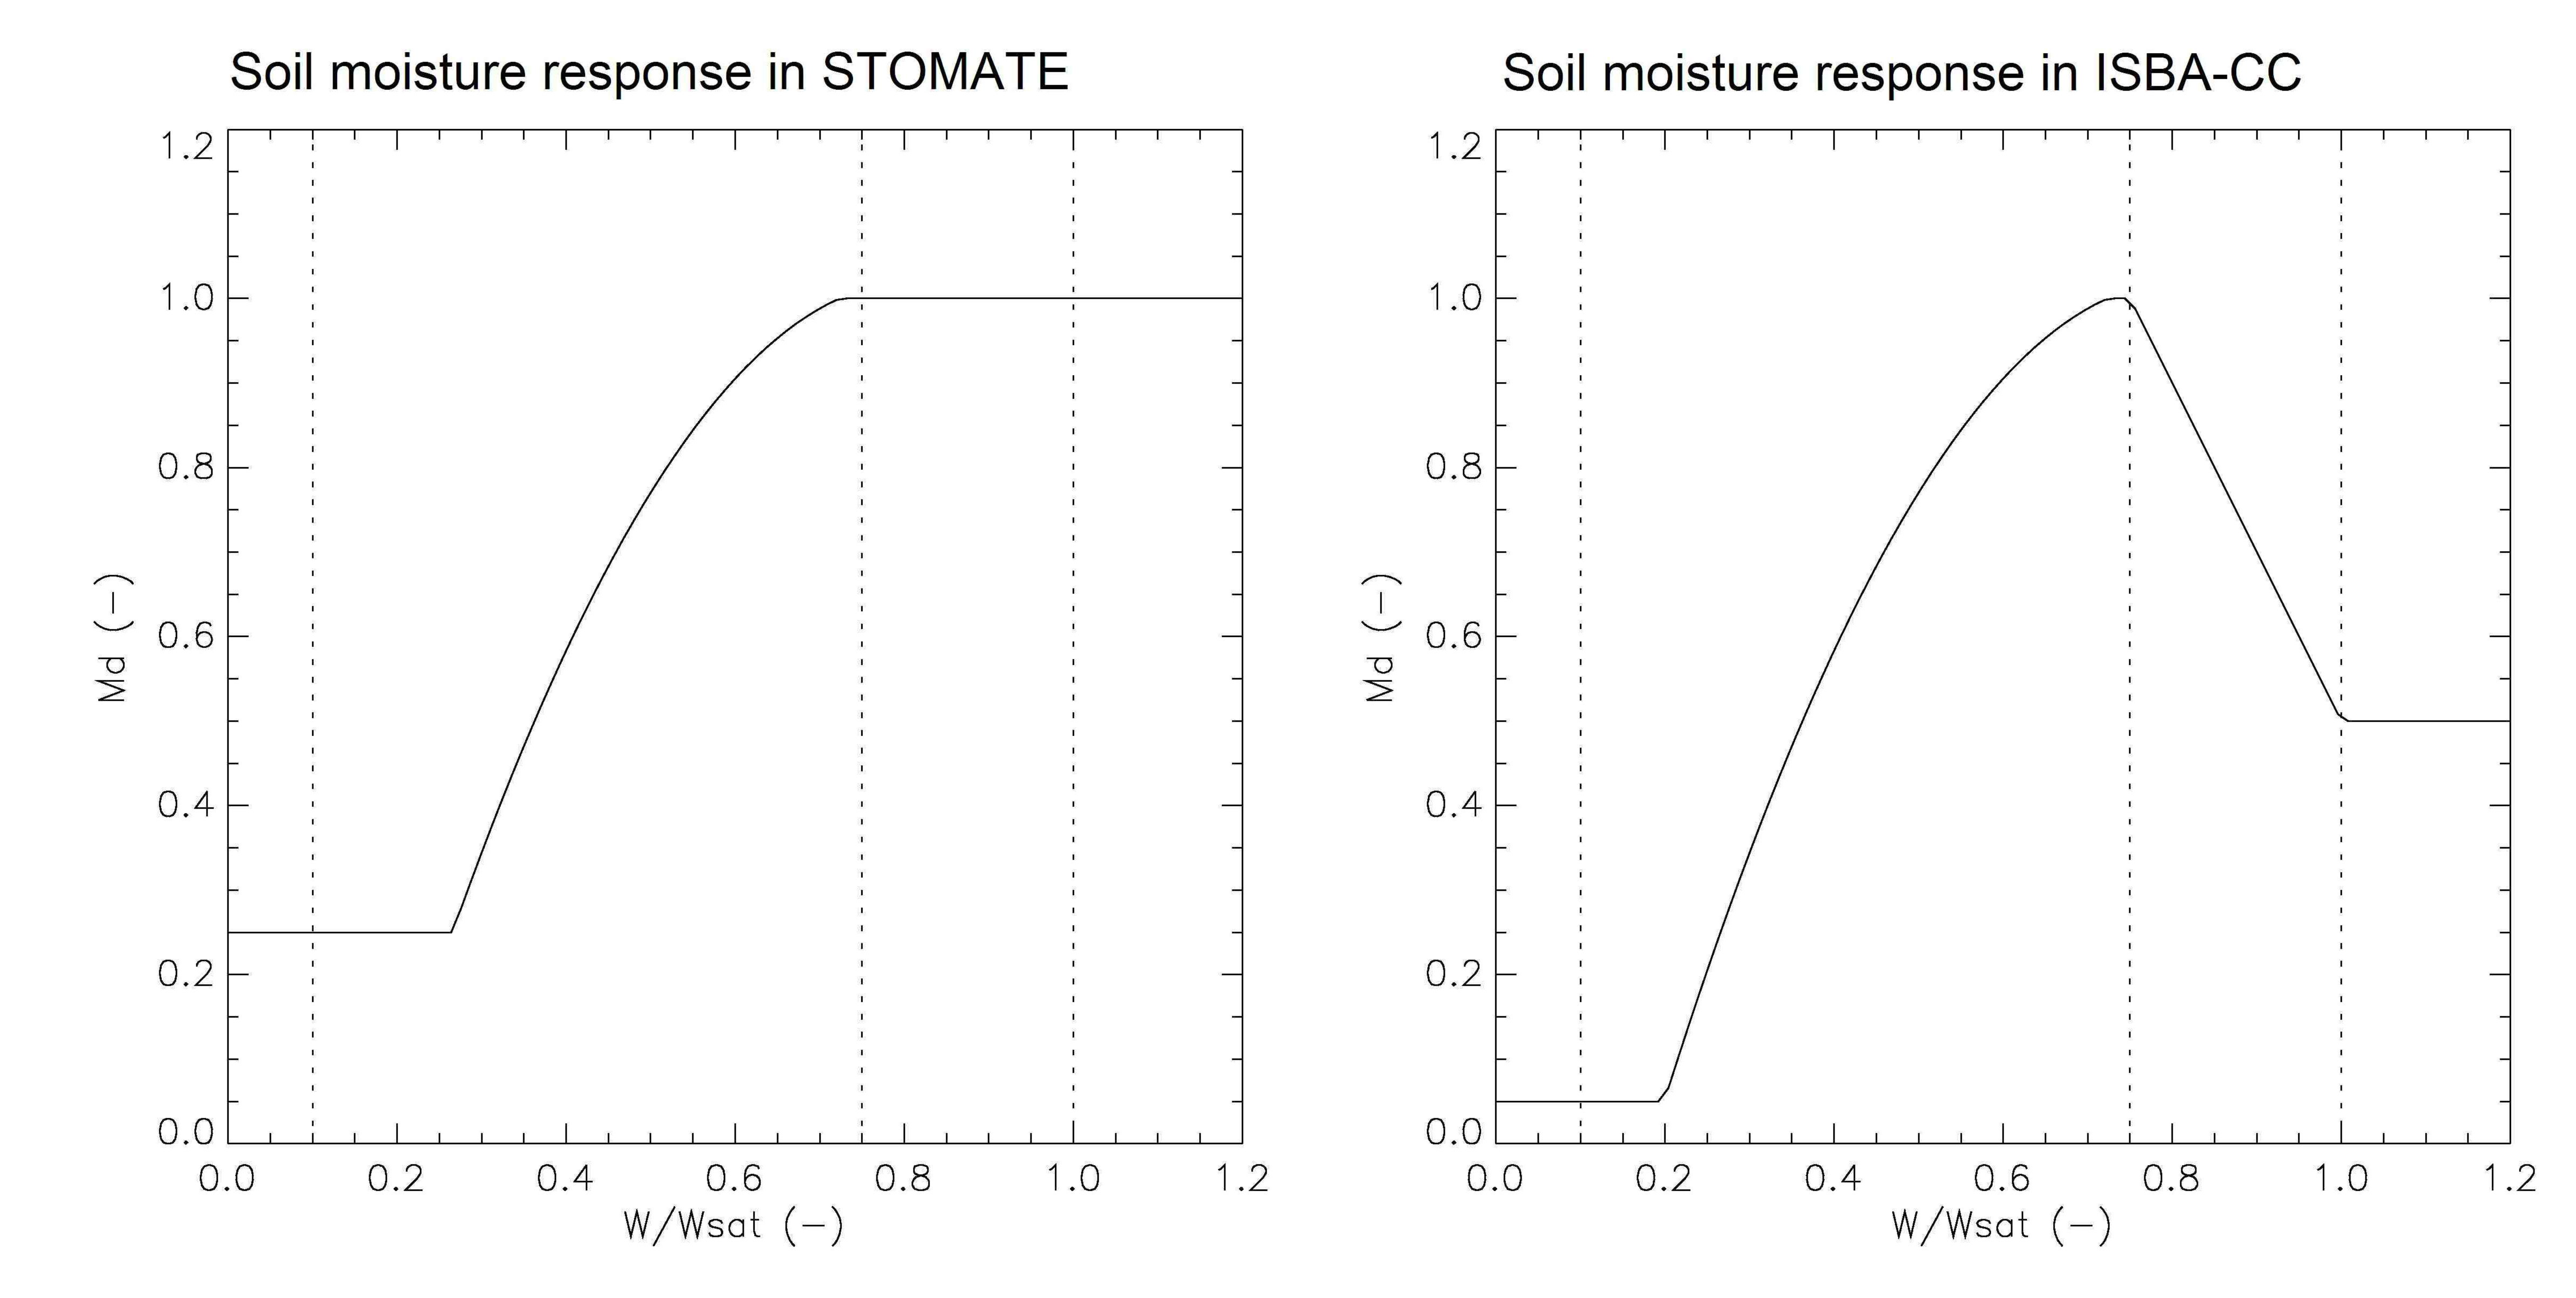
\includegraphics[width=0.9\textwidth]{\EPSDIR/trace_resp_soil_control-soilmoisture.eps}
\psfig{figure=\EPSDIR/trace_resp_soil_control-soilmoisture.eps,width=14cm}
\caption{Normalized decomposition response function to soil moisture 
       used in (left) STOMATE-ORCHIDEE and (right) ISBA-CC.
	 The three vertical dashed lines indicate (from left to right) $w_{wilt}$, 
	 $w_{fc}$ and $w_{sat}$.}
\label{fig_moist}
\end{center}
\end{figure}


Since the soil organic matter model does not represent the profile
carbon content of the soil, two soil moisture quantities are used in ISBA-CC: 
the surface soil moisture (a skin soil moisture corresponding to a thin soil layer of about 1cm) 
and the root-zone soil moisture. 
For the litter reservoirs, $w$,
$w_{wilt}$, $w_{fc}$ and $w_{sat}$ correspond to the surface soil moisture.
For the other reservoirs, $w$, $w_{wilt}$, $w_{fc}$ and $w_{sat}$ correspond to the root-zone soil moisture.


In CENTURY, the dependence of the decomposition on temperature is represented by a normalized factor, $T_d$,
driven by the average monthly temperature, according to a bell curve (Parton \etal 1987).

In STOMATE, $T_d$ is defined as:

\begin{equation}
T_d = 2 ^ {(\frac{T-30}{10})}
\end{equation}

where $T$ is soil temperature in units of $^{\circ}$C.
This formulation is used in ISBA-CC, also.

The $T_d$ values used in STOMATE and ISBA-CC are shown by Fig. \ref{fig_temp}.


%\begin{figure}[htb]
%\begin{figure}[htbp]
\begin{figure}[h]
\begin{center}
%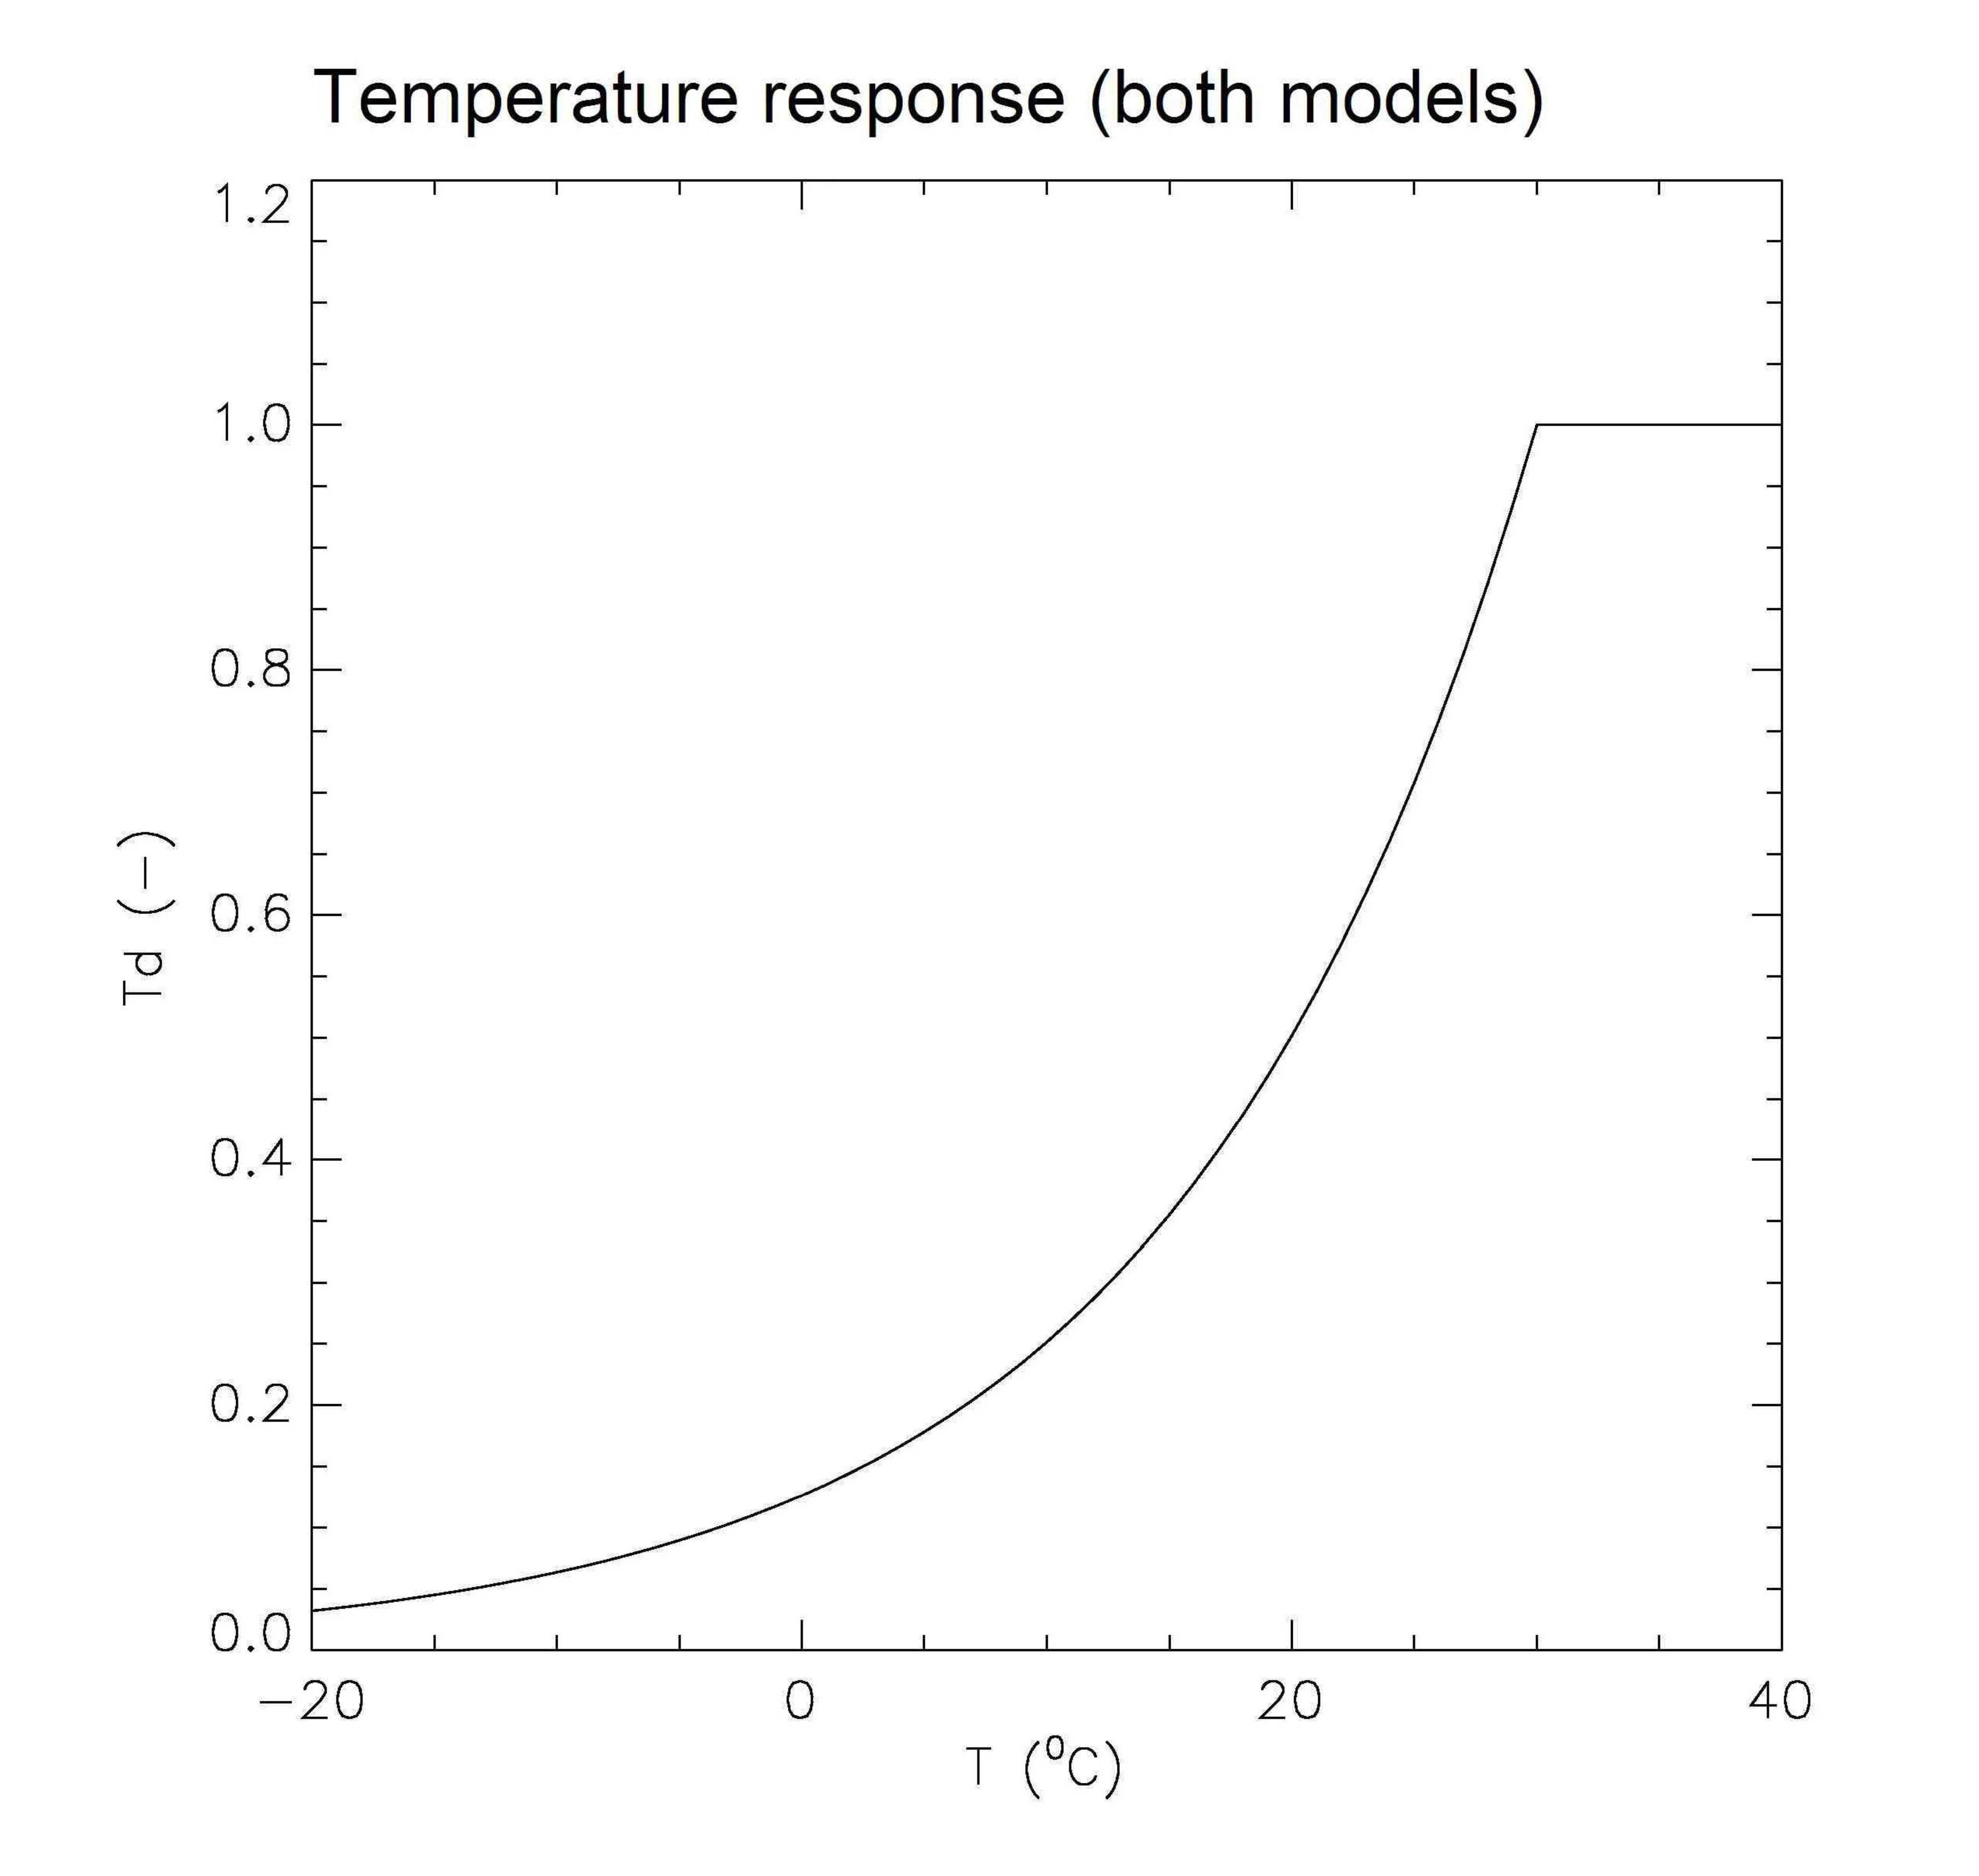
\includegraphics[width=0.9\textwidth]{\EPSDIR/trace_resp_soil_control-temperature.eps}
\psfig{figure=\EPSDIR/trace_resp_soil_control-temperature.eps,width=10cm}
\caption{Normalized decomposition response function to soil temperature 
         used in both STOMATE-ORCHIDEE and ISBA-CC.}
\label{fig_temp}
\end{center}
\end{figure}


Since the soil organic matter model does not represent the profile
carbon content of the soil, two soil temperature quantities are used in ISBA-CC: 
the surface temperature $T_s$ 
and a deep soil temperature $T_p$. 
For the litter reservoirs, $T$ = $T_s$.
For the other reservoirs, $T$ = $T_p$.


%=========================================================================================================
\subsubsection{Carbon fluxes}
%=========================================================================================================

The  decomposition of the organic matter contained in the soil carbon reservoir $i$, 
$dC_i/dt$, 
triggers various carbon fluxes (Fig. \ref{fig_soil}).
A fraction of the decomposed organic matter $f_{i,CO_2}$ is mineralized through the respiration process 
and released as CO$_2$ to the atmosphere. 
The other fraction is allocated to the other carbon pools of the soil, based on their 
resistance to decomposition. The fraction of the decomposition flux from reservoir $i$ 
to reservoir $j$ is $f_{i,j}$, and:


\begin{equation}
\sum_j f_{i,j}\ + f_{i,CO_2} = 1
\end{equation}


For the structural litter reservoirs, the decomposition supplies the respiration flux 
and the stabilisation of carbon into a soil organic matter carbon pool, either active or slow, 
depending on the lignin content of the litter and on the nature of the litter (above-ground or below-ground).
The lignin tends to reduce both the mineralization and the decomposition of the plant residues.

For the above-ground structural litter, the fractions are defined as:

\begin{equation}
\begin{tabular}{l}
$ f_{1,5} = 0.55 \: ( 1 - L_1 ) $ \\
$ f_{1,6} = 0.7 \: L_1 $ \\
$ f_{1,CO_2} = 0.45 \: ( 1 - L_1 ) + 0.3 \: L_1 $ \\
\end{tabular}
\end{equation}

where $L_1$ is the lignin fraction of the above-ground structural litter reservoir.

For the below-ground structural litter, the fractions are slightly different, in relation to 
a lower efficiency of the decomposition process to stabilize carbon into the active soil organic matter pool:

\begin{equation}
\begin{tabular}{l}
$ f_{3,5} = 0.45 \: ( 1 - L_3 ) $ \\
$ f_{3,6} = 0.7 \: L_3 $ \\
$ f_{3,CO_2} = 0.55 \: ( 1 - L_3 ) + 0.3 \: L_3 $ \\
\end{tabular}
\end{equation}

where $L_3$ is the lignin fraction of the below-ground structural litter reservoir.

The decomposition of the metabolic litter reservoirs supplies the respiration flux 
and the stabilization of carbon into the active soil organic matter carbon pool. 
The fractions are the same for above-ground and below-ground reservoirs:

\begin{equation}
\begin{tabular}{l}
$ f_{2,5} = 0.45 $ \\
$ f_{2,CO_2} = 0.55 $ \\
\\
$ f_{4,5} = 0.45 $ \\
$ f_{4,CO_2} = 0.55 $ \\
\end{tabular}
\end{equation}

The decomposition of the active soil organic matter carbon pool supplies the respiration flux 
and the slow and passive soil organic matter carbon pools, based on 
soil texture: 

\begin{equation}
\begin{tabular}{l}
$ f_{5,6} = 1 - 0.004 - ( 0.85 - 0.68 \: (f_{silt}+f_{clay}) ) $ \\
$ f_{5,7} = 0.004 $ \\
$ f_{5,CO_2} = 0.85 - 0.68 \: (f_{silt}+f_{clay}) $ \\
\end{tabular}
\end{equation}

The $f_{5,6}$ and $f_{5,CO_2}$ terms are identical to those used in CENTURY.
Note that in STOMATE, $f_{clay}$ is used instead of the $(f_{silt}+f_{clay})$ term. 

The decomposition of the slow soil organic matter carbon pool supplies the respiration flux 
and the active and passive soil organic matter carbon pools, based on soil texture: 

\begin{equation}
\begin{tabular}{l}
$ f_{6,5} = 0.42 $ \\
$ f_{6,7} = 0.03 $ \\
$ f_{6,CO_2} = 0.55 $ \\
\end{tabular}
\end{equation}

Finally, the decomposition of the passive soil organic matter carbon pool supplies the respiration flux 
and the active soil organic matter carbon pool.

\begin{equation}
\begin{tabular}{l}
$ f_{7,5} = 0.45 $ \\
$ f_{7,CO_2} = 0.55 $ \\
\end{tabular}
\end{equation}



%=========================================================================================================
%=========================================================================================================
\subsection{Description of a simulation with ISBA-CC}{Not up-to-date, new version to be released by June 2018}
%=========================================================================================================
%=========================================================================================================

ISBA-CC describes the evolution of several prognostic variables:
the plant biomass reservoirs and the soil organic matter reservoirs.
Prescribing initial or equilibrium values of these reservoirs is not easy, at both 
local and global scales. 
Indeed, accurate observations of these quantities are lacking. 
More often than not, the various biomass components are not measured separately, 
or do not correspond to the definition of the modelled compartments. 
Also, the soil carbon observations are sparse, and generally concern the first top centimeters 
of the soil, rarely below 30cm, and barely ever below 1m.

In order to avoid drifts in the carbon reservoirs, spin-up simulations must be performed, 
until equilibrium reservoir values are reached. 
Whereas the initial CENTURY model was designed to work at a monthly scale, ISBA-CC accounts for 
the diurnal cycle and is coupled with a land surface model working at the half-hourly time scale or better.
As the time scale for reaching equilibrium values is about a few hundred years for wood 
and several thousand years for the passive soil carbon pool, the spin-up simulations concern 
very long periods of time.
Therefore, the spin-up simulations cannot involve the whole coupled model. Instead, the carbon reservoir 
spin-up is performed offline, in several steps described below.

\begin{enumerate}
\item A first spin-up simulation (a few years) is performed with ISBA-CC in order to 
  initialize the soil moisture reservoirs, together with the biomass reservoirs presenting 
  a relatively high turnover such as leaves and the plant structural biomass. 
  For the woody plant types, the wood allocation terms resulting from this simulation are stored
  at a daily time step (see Section \ref{subs:isbacc_alim}).
\item An offline program produces the evolution of wood reservoirs, at a daily time step, 
  until equilibrium has been reached, using the allocation and decline terms. 
  The latter depends on the amount of carbon stored in the reservoir  
  (Section \ref{subs:isbacc_decl}), and as such must be recalculated every day.
\item A second ISBA-CC simulation is performed, in order to calculate and store daily surface and deep 
  soil temperature and soil moisture values. Also, the mortality fluxes of the plant biomass reservoirs 
  are obtained.
\item An offline program produces the evolution of the soil carbon reservoirs, at a monthly time step, 
  until equilibrium has been reached, using the mortality fluxes and the soil temperature and soil moisture values,
  based on the equations listed in Section \ref{sect:isbacc_soil}.
  The equilibrium is reached after several thousand years. It must be noted that since the use 
  of a monthly time step tends to filter out
  the variability of the surface soil moisture, the obtained equilibrium values may 
  differ from those that would have been obtained using a daily time step.
\item Finally, a last ISBA-CC simulation permits the spin-up
  of the litter reservoirs and of the active soil organic matter.
\end{enumerate}

A major shortcoming of this equilibrium method is that on an annual or multi-annual basis, the 
litter supply and the gross primary production are counterbalanced by the heterotrophic respiration, 
and by the autotrophic respiration, respectively.
Therefore, the average net carbon exchange and net primary production present null values.
This method does not permit the determination of long term land carbon sinks and sources. 
Performing more refined carbon budgets at a global scale is very difficult, as a perfect knowledge 
of the initial values of the carbon reservoirs and of the land cover/land use history is needed, 
especially for managed forests and for agricultural lands.
However, the seasonal variability of the carbon fluxes can be represented by this method, as well 
as the impact of extreme events (e.g. droughts).
Also, the equilibrium state can be used to initialize impact simulations related to the response of 
the terrestrial carbon cycle to long term perturbations.

In practise, two SURFEX namelists (NAM\_ISBA and NAM\_PREP\_ISBA\_CARBON) have to be modified before performing ISBA-CC runs.
In NAM\_ISBA, CPHOTO = 'NCB'. In NAM\_PREP\_ISBA\_CARBON, CRESPSL = 'CNT'. The former activates the 6 biomass pools, and the latter activates 
the soil heterotrophic repiration and the soil organic matter pools.
The different steps of spin-up have been coded in a script called spinup\_CC.bsh, 
available on the SURFEX web site. This script automatically perfoms the namelist
changes and the simulation repetitions needed for the spin-up. This script can be
used as a template and be adapted for specifics needs. Please note that the spin-up
procedure is designed for inputs and outputs in ASCII format. In particular, the
NetCDF, and FA formats cannot be used.



%=========================================================================================================
%=========================================================================================================
\subsection{Conclusion}
%=========================================================================================================
%=========================================================================================================

The ISBA-CC model is a new version of ISBA permitting 
the detailed simulation of the land-atmosphere carbon exchange. 
It results from the coupling between ISBA-A-gs (Calvet and Soussana, 2001) 
and the heterotrophic respiration parameterization used in ORCHIDEE (Krinner \etal 2005).
This coupling has required a number of developments.

The ISBA-A-gs allocation scheme was upgraded, in order to simulate all 
the plant biomass compartments, roots and wood in particular (Section \ref{sect:isbacc_biom}).
The principles of the initial allocation scheme, proposed by Calvet and Soussana (2001), were extended 
to the new biomass reservoirs.
All the plant respiration terms are now calculated and their sum represents the autotrophic respiration.
Also, the mortality of the biomass elements is calculated, and supplies the heterotrophic respiration module.
The latter is derived from the parameterization used in ORCHIDEE (Krinner \etal 2005), based on the CENTURY 
model (Parton \etal 1987). It simulates several soil organic matter pools (above-ground and below-ground litter,
and the decomposed organic matter), the carbon fluxes between these pools, and the CO$_2$ flux to the 
atmosphere generated by the heterotrophic respiration (Section \ref{sect:isbacc_soil}).

A few equations differ from the ORCHIDEE parameterization. 
The soil texture effect is based on the original CENTURY formulation, 
i.e. using the silt and clay fraction sum $(f_{silt}+f_{clay})$ 
instead of the mere clay fraction $f_{clay}$ in ORCHIDEE.
Also, the decomposition response to soil moisture is based on 
the saturation soil moisture value $w_{sat}$, available in ISBA simulations. 
This permits the representation of the lower decomposition rates which are observed 
in anaerobic conditions.

The added value of ISBA-CC is the calculation of the two heterotrophic and autotrophic 
respiration terms, allowing the simulation of the net primary production (NPP).
The latter describes the net carbon flux absorbed by the vegetation. 
Also, wood compartments are simulated, and even if forest management processes are not represented so far, 
forest biomass estimates can be used, to some extent, to validate the model simulations.

A complete ISBA-CC simulation has to be made in several steps, including three simulations separated 
by offline spin-up simulations of (1) the plant biomass reservoirs, and (2) the soil carbon pools.

This method produces equilibrium simulations and does not permit the determination 
of long term land carbon sinks and sources. 
However, the seasonal variability of the carbon fluxes can be represented by this method, as well 
as the impact of extreme events (e.g. droughts) and of climate change.


%---------------------------------------------------------------------------



%====================
\bibliography{surfex_scidoc}
%====================

%%%%%%%%%%%%%%%%%%%%%%%%%%%%%%%%%%%%%%%%%%%%%%%%%%%%%%%%%%%%%%%%%%%%%%%%%%%%%%%
% CONTRIBUTION TO THE SURFEX BOOK1: "Surface Processes Scheme"
% Author        : P. Le Moigne
% Original      : January 05, 2009
% Last Update   : January 05, 2009
%%%%%%%%%%%%%%%%%%%%%%%%%%%%%%%%%%%%%%%%%%%%%%%%%%%%%%%%%%%%%%%%%%%%%%%%%%%%%%%


\chapter{Surface boundary layer scheme}\label{SBL}
\minitoc
%=========================
\bibliographystyle{plain}
%=========================


\section{Introduction}

Surface atmosphere exchanges, mainly momentum, water and heat surface fluxes, drive the boundary layer evolution, and influence the formation of low level clouds and more generally the synoptic flows and climate system. The modelling of these fluxes is performed by specific surface schemes: Soil-Vegetation-Atmosphere Transfer (SVATs) schemes for vegetation (Chen \etal (1997)\nocite{Chen1997} review the vegetation schemes used in the intercomparison exercice on Cabauw grass site), urban schemes for cities (see a review in Masson (2006)\nocite{Masson2006}), or schemes dedicated to sea or ice surfaces. The degree of complexity of these schemes is wide. The simplest models are bucket models (e.g. Manabe (1969)\nocite{Manabe1969}, Robock \etal (1995)\nocite{Robock1995}), with only one water reservoir in the soil. Next are the so-called big leaf models (Deardorff (1978), Noilhan and Planton (1989)\nocite{Noilhan1989} with only one surface energy balance and no canopy. The more detailed schemes have several layers in the soil, several energy budgets (low vegetations, snow and tree canopy) and photosynthesis production to simulate the carbon cycle (see Simon \etal (2005)\nocite{Simon2005}). The same degree of variability exists in the complexity of the physical processes described in urban schemes (see Masson (2006)).

However, the present paper will not discuss on the complexity of the physical and physiological processes of the soil or plants in these schemes. The topic of this paper is to discuss the coupling of surface schemes to atmospheric models. Independantly of the complexity of the processes, two coupling methods are usually used (fig \ref{fig1}):

\begin{itemize}
\item single-layer coupled schemes: these surface schemes are forced by only one atmospheric layer (i.e. the lowest atmospheric layer of an atmospheric model, as in fig \ref{fig1}b). The surface schemes respond to atmospheric variables at this level (temperature, wind, humidity, incoming radiation, etc...) and they produce averaged upwards turbulent fluxes and radiative quantities (albedo, emissivity, surface temperature). Note that this level is physically supposed to be high enough above the surface to be in the inertial sublayer (or constant flux layer), most schemes using Monin-Obukhov theory to parameterize turbulent fluxes. These exchanges have been normalized in the Assistance for Land-surface Modelling activities (ALMA) norm (see Best \etal (2004)\nocite{Best2004} and Polcher \etal (1998)\nocite{Polcher1998}).\\
 Because of the simplicity of this type of coupling, these surface schemes can be used off-line (e.g. forced directly by observations), so that they can be used for a wide range of applications (e.g. hydrology). All schemes presented in the offline intercomparison by Chen \etal (1997)\nocite{Chen1997} are single-layer schemes. These schemes can have a separate modelling  of the soil and of the canopy, but the coupling with the atmosphere is always done at a forcing level above the canopy. The link between the forcing level and the soil/canopy to compute energy fluxes is usually done using systems of aerodynamical/stomatal resistances (as in Deardorff (1978)\nocite{Deardorff1978}), that may depend on many factors, such as plant stress or atmospheric stability.
\item multi-layer coupled schemes: these schemes are coupled with several atmospheric levels (fig \ref{fig1}c). They interact not by surface fluxes (except for the lowest level), but directly throughout the prognostic variables equations of the atmospheric model at each level. For example, drag forces by the obstacles (trees or buildings) will slow the wind and increase the turbulence, heat (water) fluxes by these obstacles will produce differential heating (moistening) between the levels. Xinmin \etal (1999)\nocite{Xinmin1999} use such a scheme coupled inline to a planetary boundary layer model to study the influence of the tree density in a forest on the air characteristic within the canopy at day and at night. Recently Simon \etal (2005)\nocite{Simon2005} built a multilayer scheme to describe precisely the water and carbon dioxyde fluxes inside the Amazonian forest. For building canopies, Martilli \etal (2002)\nocite{Martilli2002}, Coceal and Belcher (2005)\nocite{Coceal2005} and Kondo \etal (2005)\nocite{Kondo2005} are example of multi-layer schemes. The drawback of this high resolution description of the atmospheric processes is an intimate coupling of the surface scheme and the atmospheric model. Furthermore, because atmospheric layers are thin near the surface (depth of the order of 1m) to finely describe the air profile in the Surface Boundary Layer (SBL), the time step of the atmospheric model must usually be much smaller in order to insure numerical stability. \\
Such schemes are used when one wants to describe very finely the interaction between the atmosphere and the surface features. For example, low vegetation and soil will interact with air temperature near the surface (say 1m), while tree leaves exchange temperature and humidity with higher level air (with other temperature, humidity). This therefore allows a priori  a better simulation of the physical and physiological processes. Another interest of these schemes is the direct simulation of air characteristics down to the surface itself, allowing several specific applications (wind stress in forest ridges, air temperature profile between buildings, etc...).
\end{itemize}

The objective of this paper is to implement into single-layer schemes the fine description of air profiles near the ground of the multi-layer schemes. That way, the single-layer schemes will gain the explicit physical representation of the surface boundary layer thanks to additionnal air layers, and still be coupled to atmospheric models through only one layer. 

\begin{figure}[h]
\hspace*{2.cm}
\psfig{figure=\EPSDIR/fig1.eps,width=10cm}
\caption{Schematic view of surface scheme coupling: a) single-layer surface scheme forced offline. b) single-layer surface scheme forced by an atmospheric model. c) multi-layer scheme forced by an atmospheric model. Dotted arrows show the interactions between surface and coupling/atm. forcing: (a) with the forcing level, (b) the lowest atm level and (c) with all levels intersecting the canopy.\label{fig1}}
\end{figure}

%%%%%%%%%%%%%%%%%%%%%%%%%%%%%%%%%%%%%%%%%%%%%%%%%%%%%%%

\section{Theory}


\subsection{Atmospheric equations}

The atmosphere can be described by dynamical (3 wind components) and thermodynamical variables (heat content or temperature, water vapor, possibly other water phases quantities). In this study, only the Planetary Boundary Layer was considered, neglecting mean vertical velocity and horizontal turbulent fluxes. The Boussinesq hypothesis is applied for the sake of simplicity. However, the following derivation can be generalized to more complex equation systems. Only the theory is described in the main part of the paper. The numerics for implementation and coupling in models are discussed in the last section.\\

Using mean horizontal wind components ($U$, $V$), potential temperature ($\theta$) and water vapor specific humidity ($q$), without water phase changes, the equations describing the atmosphere evolution can be written as:
\begin{equation}
\left\{
\begin{array}{llllll}
\frac{\partial U}{\partial t} &=&\underbrace{- U\frac{\partial U}{\partial x} - V\frac{\partial U}{\partial y}}_{Adv}& \underbrace{-fV}_{Cor} &\underbrace{+fV_g}_{Pres.} & \underbrace{-\frac{\partial\overline{u'w'}}{\partial z}}_{Turb} \\
\frac{\partial V}{\partial t} &=&\underbrace{- U\frac{\partial V}{\partial x} - V\frac{\partial V}{\partial y}}_{Adv}& \underbrace{+fU}_{Cor}&\underbrace{-fU_g}_{Pres.} & -\underbrace{\frac{\partial\overline{v'w'}}{\partial z}}_{Turb}\\
\frac{\partial \theta}{\partial t} &=&\underbrace{- U\frac{\partial \theta}{\partial x} - V\frac{\partial \theta}{\partial y}}_{Adv}& + \underbrace{\dot{Q}}_{Diab.}  && -\underbrace{\frac{\partial\overline{w'\theta'}}{\partial z}}_{Turb} \\
\frac{\partial q}{\partial t} &=&\underbrace{- U\frac{\partial q}{\partial x} - V\frac{\partial q}{\partial y}}_{Adv}&  && -\underbrace{\frac{\partial\overline{w'q'}}{\partial z}}_{Turb} \\
\end{array}
\right.
\end{equation}


where $U_g=-\frac{1}{f\rho}\frac{\partial p}{\partial x}$ and $V_g=-\frac{1}{f\rho}\frac{\partial p}{\partial y}$ are the geostrophic wind components, $\overline{u'w'}$, $\overline{v'w'}$, $\overline{w'\theta'}$ and $\overline{w'q'}$ are the turbulent fluxes, and $\dot{Q}$ represents the diabatic sources of heat (e.g. radiative tendency). \\

In addition, a Turbulent Kinetic Energy (TKE, noted $e=\frac{1}{2}(\overline{u'^2}+\overline{v'^2}+\overline{w'^2})$) equation can be used to describe the turbulence in some atmospheric models:
\begin{equation}
\frac{\partial e}{\partial t} =\underbrace{- U\frac{\partial e}{\partial x} - V\frac{\partial e}{\partial y}}_{Adv} \underbrace{- \overline{u'w'}\frac{\partial U}{\partial z} - \overline{v'w'}\frac{\partial V}{\partial z}}_{Dyn. Prod.} +\underbrace{ \frac{g}{\theta}\overline{w'\theta_v'}}_{Therm. Prod.} - \underbrace{\frac{\partial \overline{w'e}}{\partial z}}_{Turb} -\underbrace{\epsilon}_{Diss.}
\end{equation}

where Right Hand Side terms stand for advection of TKE, dynamical production, thermal production, turbulent transport of TKE and dissipation respectively. \\

\subsection{Atmospheric equations modified by canopy obstacles}

The above equations refer to air parcels that do not interact with any obstacles. Near the surface, when one wants to take into account the influence of obstacles on the flow, these equations must be modified. In atmospheric models, this is done by adding additional terms for each variable, representing the average effect of these obstacles on the air contained in the grid mesh. One should note here that ideally, the volume of the obstacles (trees, buildings) contained into the grid mesh should be removed from the volume of air of the grid mesh. However, this significantly complexifies a lot the atmospheric model, and the approximation to keep the air volume constant even in the presence of obstacles is normally done. This simplification is also chosen here. Then, obstacles impact on the flow is parameterized as:\\

\begin{equation}
\left\{
\begin{array}{lllllll}
\frac{\partial U}{\partial t} &=&Adv& + Cor & + Pres.& + Turb(U) & + {\rm Drag_u} \\
\frac{\partial V}{\partial t} &=&Adv& + Cor& + Pres. & + Turb(V) & + {\rm Drag_v}\\
\frac{\partial \theta}{\partial t} &=&Adv& + Diab.  &&  + Turb(\theta) & + \frac{\partial \theta}{\partial t}_{canopy}\\
\frac{\partial q}{\partial t} &=&Adv&  && + Turb(q) & + \frac{\partial q}{\partial t}_{canopy} \\
\end{array}
\right.
\label{eq_complete}
\end{equation}
and 
\begin{equation}
\frac{\partial e}{\partial t} =Adv + Dyn. Prod. + Therm. Prod. + Turb  + Diss. + \frac{\partial e}{\partial t}_{canopy}
\end{equation}

where, 
\begin{itemize}
\item ${\rm Drag_u}$ and ${\rm Drag_v}$ are the drag forces (due to pressure forces against the obstacles) that slow the flow, 
\item $\frac{\partial \theta}{\partial t}_{canopy}$ is the heating/cooling rate due to the heat release/uptake by the surfaces of the canopy obstacles in the grid mesh, 
\item $\frac{\partial q}{\partial t}_{canopy}$ is the moistening/drying impact of these obstacles, 
\item and $\frac{\partial e}{\partial t}_{canopy}$ represents the TKE production due to wake around and behind obstacles as well as the additionnal dissipation due to leaves-induced small-scale turbulence.
\end{itemize}

The prescription of these terms due to the obstacle impact on the flow are parameterized differently for each multi-level surface scheme, and this is not described in detail here. Parameterizations for dynamical variables are often similar for forest canopies. Wind drag is usually parameterized as the opposite of the square of the wind, as in Shaw and Schumann (1992)\nocite{Shaw1992} or Patton \etal (2001)\nocite{Patton2001}:  ${\rm Drag_u}=- C_d a(z) U \sqrt{U^2+V^2}$ and ${\rm Drag_v}=- C_d a(z) V \sqrt{U^2+V^2}$, where $C_d$ is a drag coefficient and $a(z)$ is the leaf area density at height $z$ (this parameter can be derived from Leaf Area Index and vegetation height, assuming a normalized vertical profile of leaves distribution in the canopy). The TKE production/destruction term can be parameterized as the sum of two effects: wake production by the leaves (parameterized as proportionnal to the cubic power of wind: $\frac{\partial e}{\partial t}_{canopy} \propto C_d(U^2+V^2)^\frac{3}{2}$ as in Kanda and Hino (1994)\nocite{Kanda1994}) and the energy loss due to fast dissipation of small scale motions (leaves are of a much smaller scale than the grid mesh). The latter term is often parameterized as proportionnal to the product of wind by TKE ($\frac{\partial e}{\partial t}_{canopy} \propto -C_de\sqrt{U^2+V^2}$ as in Kanda and Hino (1994)\nocite{Kanda1994}, Shen and Leclerc (1997)\nocite{Shen1997}, Patton \etal (2003)\nocite{Patton2003}). Because of the high degree of complexity of the processes involved (and hence of possibles simplifications), parameterizations for temperature and humidity exchanges are much more variables. For example, Sun \etal (2006)\nocite{Sun2006} parameterize heating effects simply as a function of radiation vertical divergence, while more complex vegetation models, as in Park and Hattori (2004)\nocite{Park2004}, solve leaves temperature and use it to estimate at each atmospheric layer the heat and water vapor exchanges between the forest canopy and the air: $\frac{\partial \theta}{\partial t}_{canopy} \propto a(z) (\theta_l - \theta)$ and $\frac{\partial q}{\partial t}_{canopy} \propto a(z) (q_{sat}(\theta_l) - q)$, where $\theta_l$ is the leaves potential temperature and $q_{sat}$ is humidity at saturation (proportionnality coefficients depend on physiological processes of the plant).\\

For urban canopies, the same drag approach is chosen in general for the effect on wind, and only the wake production term is kept for TKE (because turbulent eddies are large behind buildings, so their dissipation is not as fast as those produced by leaves). Heat exchanges are however more complex and detailled (see Masson (2006)\nocite{Masson2006} for a review), as radiative trapping and shadows, different building heights, and sometimes even road trees are taken into account in state-of-the-art urban models. An exemple of urban canopy parameterization is given in Hamdi and Masson (2008)\nocite{Hamdi2008}.\\

As stated above, these additional terms allow a fine description of the mean variable profiles in the atmospheric model in the SBL (e.g. wind and temperature profile as a function of stability, wind speed in forest canopy, etc...) and of the flow statistics (non constant flux layer inside the canopy for example). \\

\subsection{Implementation of the SBL equations into a surface scheme}

The objective of this paper is to provide a way to implement such a description of the SBL with a lot of atmospheric layers directly into the surface scheme. Such a scheme could be used offline (figure \ref{fig2}a) or coupled to an atmospheric model (figure \ref{fig2}b). As seen by comparing with figure \ref{fig2}c, the vertical resolution is the same as with a multi-layer model. The problem is that the computation of most of the terms of the equations (advection, pressure forces, diabatic heating) requires the atmospheric model dynamics and physical parameterizations. \\

\begin{figure}[h]
\hspace*{2.cm}
\psfig{figure=\EPSDIR/fig2.eps,width=15cm}
 \caption{Schematic view of the coupling between surface scheme and SBL scheme : a) single-layer surface scheme with SBL scheme forced offline. b) single-layer surface scheme with SBL scheme forced by an atmospheric model. c) multi-layer scheme coupling (as c) in figure \ref{fig1}). Dotted arrows show the interactions between surface and SBL scheme (a and b). Upper SBL level is at same height as atmospheric forcing level.\label{fig2}}
\end{figure}


The set of equation (\ref{eq_complete}) is rewritten by separating the processes as (i) 'large scale forcing' (LS, that are solved by the atmospheric model), (ii) the turbulence and (iii) the canopy effects:

\begin{equation}
\left\{
\begin{array}{lllllll}
\frac{\partial U}{\partial t} &=&LS(U)& + Turb(U) & + {\rm Drag_u} \\
\frac{\partial V}{\partial t} &=&LS(V)& + Turb(V) & + {\rm Drag_v}\\
\frac{\partial \theta}{\partial t} &=&LS(\theta)&  + Turb(\theta) & + \frac{\partial \theta}{\partial t}_{canopy}\\
\frac{\partial q}{\partial t} &=&LS(q)&  + Turb(q) & + \frac{\partial q}{\partial t}_{canopy} \\
\end{array}
\right.\label{eq5}
\end{equation}

The TKE equation remains the same:
\begin{equation}
\frac{\partial e}{\partial t} =Adv(e) + Dyn. Prod. + Therm. Prod. + Turb  + Diss. + \frac{\partial e}{\partial t}_{canopy}
\end{equation}

To represent the SBL into the single-layer surface scheme, one considers prognostic atmospheric layers, between the surface and the forcing level of the surface scheme (that is the level that is coupled to the atmosphere). Each of these layers is represented by the wind speed, the potential temperature, the humidity and the Turbulent kinetic energy (all these variables being prognostically computed). They satisfy the set of equations (\ref {eq5}). In order to solve them, the following assumptions are made:
\begin{itemize}
\item The mean wind direction does not vary in the SBL (Rotation due to Coriolis inside the SBL is neglected).
\item The advection of TKE is negligible. This assumption is not valid for horizontal scales (and grid meshes) of the order of a few times the canopy height, as equilibrium with forcing condition above is not reached (Belcher \etal (2003)\nocite{Belcher2003}, Coceal and Belcher (2005)\nocite{Coceal2005}), but it is valid for larger scales.
\item The turbulent transport of TKE ($\overline{w'e}$) is negligible near the ground and in the SBL. This assumption is fairly valid, this term being generally important only higher in the BL .
\item Above the canopy, the turbulent fluxes are uniform with height (constant flux layer).
\item The Large Scale forcing terms ($LS(U), LS(V), LS(\theta), LS(q)$) are supposed to be uniform with height in the SBL. It is assumed, for example, that advection and pressure forces are driven by synoptic flow or by the mesoscale BL flow (e.g. sea breeze). Diabatic effects on temperature are also supposed to be uniform.
\end{itemize}

Then, the equations can be solved if the turbulent terms in the SBL (see subsection (\ref{turbs})), the canopy terms (depending on each surface scheme physics), and the (uniform with height) large scale forcing are known or parameterized. \\

Writing the equations at the forcing level ($z=z_a$), which is supposed to be above the canopy (all canopy terms are set to zero) and therefore in the constant flux layer (the turbulent fluxes are supposed to be uniform, so that the divergences of turbulent fluxes are small), large scale terms can be estimated from the temporal evolution of the variables at the forcing level:
\begin{equation}
\left\{
\begin{array}{lllllll}
\frac{\partial U}{\partial t}(z=z_a) &=&LS(U) \\
\frac{\partial V}{\partial t}(z=z_a) &=&LS(V) \\
\frac{\partial \theta}{\partial t}(z=z_a) &=&LS(\theta)\\
\frac{\partial q}{\partial t}(z=z_a) &=&LS(q)\\
\end{array}
\right.\label{eq7}
\end{equation}

In reality, the constant flux layer hypothesis supposes not a constant turbulent flux but a small variation of the turbulent flux compared to its value. The small decrease/increase of the turbulent flux can lead to tendencies of the mean variables. However, this small variation is generally relatively uniform in the whole boundary layer (e.g. uniform heating of the convective boundary layer). This impact of the fluxes at the scale of the whole BL is included in the LS terms. \\

\subsection{Boundary conditions}

Finally, one obtains (using only one wind component, as the wind does not veer with height in the SBL):

\begin{equation}
\left\{
\begin{array}{lllllll}
\frac{\partial U}{\partial t} &=&\frac{\partial U}{\partial t}(z=z_a)& + Turb(U) & + {\rm Drag_u} \\
\frac{\partial \theta}{\partial t} &=&\frac{\partial \theta}{\partial t}(z=z_a)&  + Turb(\theta) & + \frac{\partial \theta}{\partial t}_{canopy}\\
\frac{\partial q}{\partial t} &=&\frac{\partial q}{\partial t}(z=z_a)&  + Turb(q) & + \frac{\partial q}{\partial t}_{canopy} \\
\end{array}
\right.\label{eq9}
\end{equation}
And
\begin{equation}
\frac{\partial e}{\partial t} = Dyn. Prod. + Therm. Prod. + Diss. + \frac{\partial e}{\partial t}_{canopy} \label{tke}
\end{equation}

The surface condition for the wind equation is given by the turbulent flux at the surface $\overline{u'w'}(z=0)$. The value at the top of the SBL scheme is given by wind at forcing level: $U=U(z=z_a)$. \\
The surface condition for the potential temperature equation is given by the turbulent flux at the surface $\overline{w'\theta'}(z=0)$. The value at the top is given by the temperature at forcing level: $\theta=\theta(z=z_a)$. \\
The surface condition for the humidity equation is given by the  turbulent flux at the surface $\overline{w'q'}(z=0)$. The value at the top is given by humidity at forcing level: $q=q(z=z_a)$. \\

The turbulent fluxes at the surface are computed by the surface scheme, using the atmospheric variables of the lowest level of the SBL (and not at the usual forcing level at $z_a$). The exact formulation depends on the surface scheme used. For example, a lot of (1 layer) surface schemes use to compute the surface heat (vapor)  flux a formulation with exchange coefficients $C_h$ (including a dependancy with stability), surface and air temperatures (humidity) ($\overline{w'\theta'}(z=0)=C_h (\theta_s - \theta_a)$). With the SBL scheme, $\theta_a$ is the temperature at first SBL level, and the stability in the lowest layer in near neutral (because of the proximity to the ground -we used 50cm as first layer-).\\

There is no need of boundary condition for the TKE at the surface or at the forcing level, as no vertical gradient of TKE is used. The only term that needs special computation near the surface is the Dynamical production term, as it uses a vertical gradient of mean wind. \\

\subsection{Turbulence scheme\label{turbs}}

One turbulence scheme is of course needed in the SBL. A TKE turbulence scheme, developed by Cuxart \etal (2000)\nocite{Cuxart2000}, is chosen here. The mixing length is computed as in Redelsperger \etal (2001)\nocite{Redelsperger2001}. Mixing and dissipative length scales are not equal, in order to represent accurately the dissipation modification due to the -1 power law of the turbulence in the SBL. Other turbulence schemes may be used.\\

A summary of the turbulence scheme is given below:
\begin{equation}
\left\{
\begin{array}{lllllll}
\overline{u'w'}&=& - C_u l\sqrt{e}\frac{\partial U}{\partial z} \\
\overline{w'\theta'}&=& - C_{\theta}l\sqrt{e}\frac{\partial \theta}{\partial z} \\
\overline{w'q'}&=& - C_{q} l\sqrt{e}\frac{\partial q}{\partial z} \\
\frac{\partial e}{\partial t} &=& \underbrace{- \overline{u'w'}\frac{\partial U}{\partial z}}_{Dyn. Prod.} +\underbrace{ \frac{g}{\theta}\overline{w'\theta_v'}}_{Therm. Prod.} -\underbrace{C_\epsilon \frac{e^{\frac{3}{2}}}{l_\epsilon}}_{Diss.} + \frac{\partial e}{\partial t}_{canopy}\\
\end{array}
\right.
\end{equation}

with $C_u=0.126$, $C_\theta=C_q=0.143$, $C_\epsilon=0.845$ (from Cheng \etal (2002)\nocite{Cheng2002} constants values for pressure correlations terms and using Cuxart \etal (2000)\nocite{Cuxart2000} derivation).
The mixing and dissipative lengths, $l$ and $l_\epsilon$ respectively, are equal to (from Redelsperger \etal (2001)\nocite{Redelsperger2001}, $\alpha=2.42$) :
\begin{equation}
\left\{
\begin{array}{lllllll}
l&=&\kappa z/[\sqrt{\alpha}C_u  \phi_m^2(z/L_{MO})\phi_e(z/L_{MO})]^{-1}&\\
l_\epsilon&=&l \alpha^2 C_\epsilon / C_u / (1-1.9z/L_{MO}) & {\rm if \hspace*{1.cm}z/L_{MO}<0}\\
l_\epsilon&=&l \alpha^2 C_\epsilon / C_u / (1-0.3\sqrt{z/L_{MO}}) & {\rm if\hspace*{1.cm} z/L_{MO}>0}\\
\end{array}
\right.
\end{equation}
Where $L_{MO}$ is the Monin-Obukhov length, $\phi_u$ and $\phi_e$ the Monin-Obukhov stability functions for momentum and TKE. \\

%%%%%%%%%%%%%%%%%%%%%%%%%%%%%%%%%%%%%%%%%%%%%%%%%%%%%%%

\section{conclusion}

A formulation allowing to include prognostic atmospheric layers in offline surface schemes is derived from atmospheric equations. The interest of this approach is to use the advanced physical description of the SBL-canopy interactions that was available only in complex coupled multi-layer surface schemes. The coupling only occurs at the bottom level of the atmospheric model that should be coupled above the surface+SBL scheme. Variables that must be exchanged are: incoming radiation and forcing level air characteristics towards the surface scheme, upward radiative and turbulent fluxes from it. The air layers prognostically simulated with the SBL scheme take into account:

\begin{itemize}
\item The term that is related to large-scale forcing (e.g. advection). The detail of this term is not known by the SBL scheme. The evolution of the air characteristics at the forcing level is supposed to take into account all these large-scale forcing terms.
\item The turbulent exchanges in the SBL (including in the canopy, if any). They will modify vertical profiles in the SBL. For example, the logarithmic profile of wind is directly induced by these turbulent fluxes, and is well reproduced by the SBL scheme.
\item The drag and canopy forcing terms. These are computed for each layer, due to the interaction between air and the canopy. These exchanges have to be modeled by the surface scheme to which the SBL scheme is coupled. In the present paper, for forests, it takes into account the dynamical terms: drag and impact on Tke.
\end{itemize}

The possible applications of a SBL scheme included in surface schemes can be:
\begin{itemize}
\item a more physical determination of standard 2m variables and 10m wind. It can be seen as a drastic increase of the vertical resolution of the atmospheric models near the ground, without the drawback of a smaller time step (that would be necessary to resolve the advection on a very fine grid). Furthermore, because the additional air layers are not handled by the atmospheric model, the SBL scheme (associated to a surface single-layer scheme) is easy to couple with Numerial Weather Prediction or research atmospheric models.
\item a better description of the turbulent exchanges and the stability in the SBL, including over complex terrain, for low-level flow and dispersion studies near the surface. As future applications, the dispersion processes in presence of canopy (e.g. chemistry vertical diffusion in urban areas) could then be more accurately simulated.
\item the inclusion of the detailed physics of the multi-layer schemes (e.g. the interactions of forest or urban canopy with atmospheric layers in the SBL) into single-layer schemes. 
\end{itemize}

%%%%%%%%%%%%%%%%%%%%%%%%%%%%%%%%%%%%%%%%%%%%%%%%%%%%%%%

\newpage
\section{\bf{Appendix}: Vertical and temporal discretization}

\subsection{Vertical discretization}

The vertical grid for the SBL scheme is a staggered grid (figure \ref{fig3}). Historical variables ($U$, $\theta$, $q$, $e$) are defined on 'full' levels. The temporal evolution terms due to canopy obstacles (${\rm Drag_u}$, $\frac{\partial \theta}{\partial t}_{canopy}$, $\frac{\partial q}{\partial t}_{canopy}$, $\frac{\partial e}{\partial t}_{canopy}$) are also located on these full levels. The turbulent fluxes computed by the SBL scheme are computed on the 'flux' levels, staggered between the full levels. The height of full levels is exactly at middle height between half levels. Note that the grid can be (and is most of the time) stretched, with a higher resolution near the ground. The ground is the first flux level (to be consistent with the boundary condition provided: the surface turbulent fluxes). The atmospheric forcing level is the upper full level (to be consistent with the upper boundary condition). \\

\begin{figure}[h]
\hspace*{2.cm}
\psfig{figure=\EPSDIR/fig3.eps,height=20cm}
\caption{Schematic view of the vertical discretization for the SBL scheme. Plain lines are full levels. Dotted lines are flux levels. \label{fig3}}
\end{figure}


\subsection{Temporal discretization}

For any variable $X$ ($U$, $\theta$, $q$ or $e$), the evolution equation can be written as:
\begin{equation}
\frac{\partial X}{\partial t} = \frac{\partial X}{\partial t}(z=z_a) - \frac{\partial F(\frac{\partial X}{\partial z})}{\partial z} + For(X)
\end{equation}
where $F$ is the turbulent flux for $X=[U,\theta,q]$, and $For$ contains  canopy forcing terms ($\frac{\partial X}{\partial t}_{canopy}$ for $X=[U,\theta,q,e]$) and other RHS forces for $X=[e]$. Note that the turbulent flux terms $F$ depend formally on the vertical derivative of the variable ($\frac{\partial X}{\partial z}$) while canopy forces and RHS TKE forces depend on the variable itself ($X$). \\

In order to satisfy the stability of the SBL scheme at large time-steps, an implicit solving is performed. If the coupling at the atmospheric level is explicit, the atmospheric forcing is not modified in the current time-step by the SBL and surface schemes (i.e. $\frac{\partial X}{\partial t}(z=z_a)$ does not change during the SBL solving). Of course, the atmosphere will further evolve in response to the turbulent SBL fluxes (through the atmospheric model turbulence parameterization). In these conditons, the SBL implicit solving writes:
\begin{equation}
\frac{X^+ - X^-}{\Delta t} = \frac{\partial X}{\partial t}^-{(z=z_a)} - \frac{\partial F}{\partial z}^- - \frac{\partial \frac{\partial F}{\partial z}}{\partial \frac{\partial X}{\partial z}}^- \times \left(\frac{\partial X}{\partial z}^+-\frac{\partial X}{\partial z}^-\right) + For^- + \frac{\partial For}{\partial X}^- \times(X^+-X^-)
\label{disc}
\end{equation}
Where $\Delta t$ is the time step, $^-$ subscript stands for previous time-step variable (known), and $^+$ subscript for the future time-step variable (which one seeks to calculate). Such an implicit scheme leads to a linear system linking all variables at each level to those from the levels below and above (due to the vertical gradient at instant $^+$). This system is tridiagonal, and easy to solve numerically. \\


\subsection{Implicit coupling with the atmospheric model}

It may be necessary in some atmospheric models (essentially due to very long time steps - half an hour- and the turbulence scheme used in the atmospheric model) to couple implicitly the surface (including the SBL scheme here) and the atmosphere. First RHS term in Equation \ref{disc} is now equal to $[X_{(z=z_a)}^+ -X_{(z=z_a)}^-]/\Delta t$. The atmospheric variable at time $^+$ is modified by the surface flux at the forcing level. It is formalized by Best \etal (2004)\nocite{Best2004} : $X_{(z=z_a)}^+ = A \times F_{(z=z_a)}^+ + B$ (where A and B are known). Therefore,  Equation \ref{disc}, in case of implicit coupling with the atmosphere, writes:
\begin{equation}
\begin{array}{ll}
\frac{X^+ - X^-}{\Delta t} =& \frac{B-X{(z=z_a)}^-}{\Delta t} + \frac{A}{\Delta t}\times \left\{ F^-_{(z=z_a)}+ \frac{\partial F}{\partial (\frac{\partial X}{\partial z})}^-{\scriptsize{(z=z_a)}}\times \left(\frac{\partial X}{\partial z}^+{\scriptsize{(z=z_a)}}-\frac{\partial X}{\partial z}^-{\scriptsize{(z=z_a)}}\right)\right\}  \\
&- \frac{\partial F}{\partial z}^- - \frac{\partial \frac{\partial F}{\partial z}}{\partial \frac{\partial X}{\partial z}}^- \times \left(\frac{\partial X}{\partial z}^+-\frac{\partial X}{\partial z}^-\right) + For(X)^- + \frac{\partial For}{\partial X}^- \times(X^+-X^-)
\end{array}
\end{equation}
This is still a linear system involving variables at future time step at all levels of the SBL scheme, but this system is no longer tridiagonal, because the term $\frac{\partial X}{\partial z}(z=z_a)^+$ (i.e. at upper SBL level) influences directly the variable $X^+$ at each level. However, such a system is still resolvable, showing the generality of the SBL scheme method proposed here.

%====================
\bibliography{surfex_scidoc}
%====================

%%%%%%%%%%%%%%%%%%%%%%%%%%%%%%%%%%%%%%%%%%%%%%%%%%%%%%%%%%%%%%%%%%%%%%%%%%%%%%%
% CONTRIBUTION TO THE SURFEX BOOK1: "Surface Processes Scheme"
% Author        : P. Tulet
% Original      : January 05, 2009
% Last Update   : January 05, 2009
%%%%%%%%%%%%%%%%%%%%%%%%%%%%%%%%%%%%%%%%%%%%%%%%%%%%%%%%%%%%%%%%%%%%%%%%%%%%%%%

\chapter{Chemistry and aerosols}
\minitoc
%=========================
\bibliographystyle{plain}
%=========================

\section{Dust aerosols}

Dust is mobilized from dry desert surfaces when the wind friction 
speed reaches a threshold wind friction speed of approximately
0.2 m/s. Dust is an important aerosol with annual global
 emissions ranging from 1000 to 3000 $Tg~yr^{-1}$ and average global
load around 10-30 $Tg$ (Zender \etal (2004)\nocite{Zender2004}).

Dust is mobilized by two related processes called saltation and 
sandblasting. Saltation is the horizonal movement of soil grains in a turbulent
near surface layer. Sandblasting is the release of fine dust when 
the saltating grains hit the surface. Several papers document these two
processes. (Marticorena and Bergametti (1995)\nocite{Marticorena1995} and references therein describe the physics
of saltations, and Shao \etal (1993)\nocite{Shao1993} describe the physics of sandblasting.


\subsection{Implementation in the Externalized surface}

The dust fluxes are calculated using the Dust Entrainment And Deposition
(DEAD) model (Zender \etal (2003)\nocite{Zender2003}). This model is based on Marticorena and Bergametti (1995).
The dust fluxes are calculated consistently with the ISBA soil surface
scheme. Table \ref{tbl:input} gives an overview of the main input to the dust 
production model.


\begin{table*}[htb]
\caption{ISBA variables used by the dust module \label{tbl:input}}
\begin{tabular}{|c|c|c|}
\hline
PARAMETER            &  EFFECT ON DUST EMISSION  & REFERENCE    \\
\hline
\hline
wind friction speed  & Increase emissions          & Marticorena and Bergametti (1995) \\
\hline
Soil moisture        & Inhibit emissions           & Fecan \etal (1999)\nocite{Fecan1999}       \\
\hline
Vegetation fraction  & Inhibit emissions           & Marticorena and Bergametti (1995)\\
\hline
Surface roughness    & Inhibit emissions           & Laurent \etal (2005)\nocite{Laurent2005} \\
\hline
Surface texture      & Soil sizes $ > ~50 {\mu}m$  &                       \\
                     &  increase saltation flux    & Iversen and White (1982)\nocite{Iversen1982}        \\
\hline 
\end{tabular}
\end{table*}


\subsection{Features of the model}

%plm=======================================================================================
\subsubsection{Emission process}
The production of desert aerosols follows in fact the sandblasting process
following the bombing of the aggregates present at the surface by particles in saltation
(Figure \ref{fig_chap5_1}). These processes depend on both weather conditions and surface states.
 Indeed, the kinetic energy of the grains caused by saltation is used in
shocks induced by these particles, when they fall to the ground to release and eject fine
particles constituting aggregates (Gillette and Goodwin (1974)\nocite{Gillette1974}, Gomes \etal (1990)\nocite{Gomes1990}). The
resistance to wrenching, concerns soil properties like the gravity force and the
inter-particle forces.
Moreover, emission of aerosols is a threshold phenomenon: it occurs only when the wind
friction force exerted on soil grains becomes greater than the forces that
maintain them to the ground. When this threshold is exceeded, the soil grains start
moving horizontally. The smallest particles can be suspended
in the atmosphere and constitute the desert aerosol.
The production intensity of fine particles thus depends on the ratio between the transfered kinetic energy
flow and the cohesion forces of the particles forming the aggregates.

\begin{figure}[h]
\begin{center}
\psfig{figure=\EPSDIR/fig_chap5_1.eps,width=10cm}
\caption{illustration of the two main processes involved in the emission of aerosols desert (saltation and sandblasting) when the
erosion threshold is exceeded. \label{fig_chap5_1}}
\end{center}
\end{figure}

Once the particle is injected into the atmosphere, the forces to which it is subjected will
control its suspension. It is generally accepted, given the balance of forces, that only
particles with a diameter less than about 20 \textmu m can be transported (Nickling (1994)\nocite{Nickling1974}). 
Those fine particles, named aerosols, constitute the main part of the vertical flow of
desert aerosol ($F$). This vertical flow is defined as the mass of particles crossing per unit of time
a unitary surface parallel to the surface.

\subsubsection{Parameterization of the friction velocity}
Wind is the driving force in the aerosols desert generating process. The
ground surface opposes the air flow and slows the air mass at its base. The surface wind
is very sensitive to changes in surface characteristics at small
scale. These changes may be due, for example, to the presence of vegetation or
rocks. In the first few meters of the atmosphere, a surface boundary layer (CLS)
develops, in which the horizontal component of the wind speed has a
vertical gradient whose intensity depends on the ability of the soil surface to slow the
flow (Figure \ref{fig_chap5_2}). For a laminar flow over a horizontal surface, the
shear constraint ($\tau$) exerted by the wind on the surface is connected to the vertical gradient
of the wind speed ($U$) by:

%eq1
\begin{equation}
\tau = \mu~~\frac{\partial U}{\partial Z}
\end{equation}
	
Where μ is the air dynamic viscosity coefficient and Z the height above the ground.

\begin{figure}[h]
\begin{center}
\psfig{figure=\EPSDIR/fig_chap5_2.eps,width=10cm}
\caption{Representation of the effect of soil on the airflow and of the shear stress $\tau$ 
exerted by the flow on the ground. \label{fig_chap5_2}}
\end{center}
\end{figure}


The shear constraint can also be expressed in terms of friction wind speed
$U_*$, which is usually the physical quantity used to quantify
friction forces exerted by wind on a surface:

%eq2
\begin{equation}
\tau = \rho_{a}~U_{*}
\end{equation}


Where $\rho_{a}$ is the air density.
Under conditions of thermal neutrality, $U_*$ can be determined from the wind speed
$U$ at a height $z$ from the ground and the height of aerodynamic roughness ($Z_0$) using a
wind speed logarithmic profile (Priestley (1959)\nocite{Priestley1959}:

%eq3
\begin{equation}
U(Z) = \frac{U_*}{\kappa}\ln(\frac{z}{Z_0})
\end{equation}


Where $\kappa=0.4$ is the Von Karman constant. \\
Physically, $Z_0$ reflects the length scale of the sink of air momentum
induced by the surface roughness. More specifically, $Z_0$ represents quantitatively the effect
of erodible elements (soil grains) or non-erodible ones (rocks or vegetation) on the transfer
of wind energy to the surface.

\subsubsection{Friction velocity threshold }

The resistance of the surface on the motion is represented by the 
friction velocity threshold $U_{*_t}$. Indeed, the friction velocity threshold $U_{*t}$ controls both the frequency and
the intensity of emissions of aerosols desert, so it is important to parameterize carefully
$U_{*_t}$ and give special attention to obtain the quantities it depends on.
The erosion threshold is mainly computed from the soil grains diameter $D_p$, the surface roughness
($Rug$) and the soil moisture ($w$).
The friction velocity threshold is expressed as:

%eq4
\begin{equation}
U_{*_t} = U_{*_t}(D_p) \cdot F(Rug) \cdot F(w)
\end{equation}


	
$U_{*_t}(D_p)$: depends on the friction speed with the diameter of soil grains.
$F(Rug)$ and $F(w)$: weighting functions of the influence of roughness and soil moisture.
Under idealized conditions, ie for a smooth surface and a loose and dry soil, the
friction velocity threshold $U_{*_t}(D_p)$ can be determined using the formulation of
Marticorena and Bergametti (1995), which consists in adjusting an empirical expression
as a function of the particle diameter. Under standard atmospheric conditions
($\rho_a = 0.00123 g \cdot cm^{-3}$, $\rho_p = 2.65 g \cdot cm^{-3}$), the friction velocity threshold $U_{*_t}(D_p)$ is
given by:

%eq5
%U_{*_{t}}(D_p) = \left [ \frac{0.1666681\rho_{p} g D}{-1+1.928 {Re_{*_t}}^{0.0922}} \left ( 1+ \frac{6\times 10^{-7}}{\rho_{p} g D^{2.5}} \right ) \right ] ^{1/2} \rho ^{-1/2} \hspace{1cm}, 0.03\leq Re_{*_t} \leq 10 \\
\begin{eqnarray}
U_{*_{t}}(D_p) = \frac{0.129 K}{ { \left ( 1.928 {Re_{*_t}}^{0.092} \right ) }^{0.5}} \hspace{1cm}, 0.03\leq Re_{*_t} \leq 10 \\
U_{*_{t}}(D_p) = 0.129  K \left [ 1-0.0858 \exp \left ( -0.0617 \left ( Re_{*_t}-10 \right ) \right ) \right ] \hspace{0.1cm}, {Re_{*_t}} > 10 
\end{eqnarray}

Where $Re_{*_t} = U_{*_t} D_p / \nu$ is the Reynolds number threshold ($\nu = 0.157~cm^{2}s^{-1}$: kinematic viscosity) \\ \\
and: $K = \left ( \frac{\rho_{p} g D_p}{\rho_{a}} \right ) ^{0.5} \left ( 1+\frac{0.006}{\rho_{p} g {D_p}^{2.5}} \right ) ^{0.5}$ \\ \\
%The friction velocity threshold is calculated in the code by the routine "wnd_frc_thr_slt_get which
%is in the module mode_dstmblutl.F90. 
The optimal diameter of the particle is equal to 75 \textmu m.

\subsubsection{Influence of soil moisture on friction velocity threshold}

The presence of interstitial water between soil grains has the effect of increasing the
cohesion of the soil, thus increasing the friction velocity threshold. This increase is
integrated in the module DEAD from the parameterization developed by Fecan \etal (1999). 
The proposed equation, expresses the threshlod increase, under wet conditions $U_{*_{tw}}$
compared to that in dry conditions.

%eq7 et eq8

\begin{eqnarray}
U_{*_{tw}} = U_{*_{t}} ~~~~~~~~~~ for~ w ~ < ~ w^{'} \\
U_{*_{tw}} = U_{*_{t}} {\left [ 1+1.21(w-w^{'})^{0.68} \right ]} ^{0.5} ~~ for~ w ~ > ~ w^{'}
\end{eqnarray}



With:
$w$: mass soil moisture (\% mass water / mass dry soil).
And soil moisture threshold is given by: 

%eq9
\begin{equation}
w^{'} = 0.17 (\%clay) + 0.14 (\%clay)^{2}
\end{equation}

%The effect of soil moisture on friction velocity threshold is treated by the
%routine "frc_thr_ncr_wtr_get" in module "mode_dstmblutl.F90.

\subsubsection{Aerodynamical roughness height}

The effects of the internal boundary layer (IBL) on friction velocity threshold, due to the presence of stones,
is set in DEAD scheme by Marticorena and Bergametti (1995). The energy distribution is defined in this parameterization as the
ratio between the IBL shear friction and the total shear friction of the surface boundary layer (SBL). This ration is given by:

%eq10
\begin{equation}
f_{eff}(Z_0,Z_{0s}) = 1 - \left [ \ln(Z_0/Z_{0s}) / \ln(0.35(10/Z_{0s})^{0.8}) \right ]
\end{equation}

	
$Z_{0s} = 33.3 \times 10^{-6}~m$: roughness length of the smooth surface \\
$Z_0 = 100.0 \times 10^{-6}~m$: roughness length of the erodible surface\\
The friction velocity threshold is expressed as:

%eq11
\begin{equation}
U_{*_t}(D_p,Z_0,Z_{0s}) = \frac{U_{*_t}(D_p)}{f_{eff}(Z_0,Z_{0s})}
\end{equation}

%This ratio is calculated by the routine "frc_thr_ncr_drg_get" in the module
%"Mode_dstmblutl.F90.

\subsubsection{Surface flux}

The horizontal saltation flux ($G$) is calculated in module DEAD through the
White (1979)\nocite{White1979} relationship :

%eq12
\begin{equation}
G = c \cdot \frac{\rho}{g}{U_*}^{3} \left ( 1-\frac{U_{*_t}}{U_{*}} \right ) \left (  1+\frac{U_{*_t}}{U_{*}} \right )
\end{equation}

With $c=2.61$. The ratio between the vertical flux and the horizontal flux is a function of clay content.
For contents between 0 and 20\%, this ratio is :

%eq13
\begin{equation}
\alpha = \frac{F}{G} = 100 \exp { \left [  ( 13.4 (\%clay) - 6 ) \times \ln(10) ~\right ] }
\end{equation}

	
In the DEAD  module, the fraction of clay is considered constant and is equal to 20\%.
The final vertical flux is averaged by a pre-determined factor equals to 0.0021 and by the sand fraction.

%plm=======================================================================================

\subsubsection{Mass flux repartition}
Upon Alfaro and Gomes (2001)\nocite{Alfaro2001} the mass flux is partitioning on the different modes upon  the surface friction velocity. More the
collision energy is strong more the dust aggregates can be separates into small particles.
In surfex, two possibilities are offered. Users can fix the partitioning or the mass flux on the differents modes considered, or compute automatically this partitioning upon the ISBA friction velocity.
In this latter case, Alfaro and Gomes (2001)\nocite{Alfaro2001} gives the following partitionning:
\begin{itemize}
\item u* less than 0.32 $m.s^{-1}$, all particles are emitted in the coarse mode.
\item u* at 0.42 $m.s^{-1}$,  63 \% of the mass flux is in the bigger coarse mode (D=14.2 $\mu m$) ,  36 \% in the lower coarse mode (D=6.7 $\mu m$), and 1 \% in the accumulation mode (D=1.5 $\mu$ m)
\item u* at 0.50 $m.s^{-1}$,  49 \% of the mass flux is in the bigger coarse mode (D=14.2 $\mu m$) ,  43 \% in the lower coarse mode (D=6.7 $\mu m$), and 8 \% in the accumulation mode (D=1.5 $\mu$ m)
\item u* at 0.66 $m.s^{-1}$,  9 \% of the mass flux is in the bigger coarse mode (D=14.2 $\mu m$) ,  76 \% in the lower coarse mode (D=6.7 $\mu m$), and 15 \% in the accumulation mode (D=1.5 $\mu$ m)
\end{itemize}
Between these friction velocities values, the mass flux partitioning is linearly interpolated.

\section{Sea Salt emission}
Sea salt aerosols are produced as film and jet droplets when bubbles, entrained in the water by breaking waves, disrupt the sea surface (Blanchard, 1983), and at winds speeds exceeding about 9 $m.s^{-1}$, by direct disruption of the wave tops (spume droplets) (Monahan \etal (1983)\nocite{Monahan1983}).

Sea Salt emission are parameterized upon the  formulation of Vignati \etal (2001)\nocite{Vignati2001} (effective source function) or upon a lookup table defined by Schulz \etal (2004)\nocite{Schulz2004}.
Vignati \etal (2001) gives a formulation of particles emission upon the wind at 10 meters as:
\begin{itemize}
\item $F(R=0.2 \mu m) = 10^{0.09 U_{10m} + 0.283} particles.cm^{-2}.s^{-1}$ 
\item $F(R= 2 \mu m) = 10^{0.0422 U_{10m} + 0.288} particles.cm^{-2}.s^{-1}$
\item $F(R= 12 \mu m) = 10^{0.069 U_{10m} - 3.5} particles.cm^{-2}.s^{-1}$
\end{itemize}

\section{Dry deposition of gaseous species}

The removal of gases from the atmosphere by turbulent transfer and uptake at
the surface is defined as dry deposition. This process enables some
chemically reactive gases to be efficiently removed from the atmosphere. 
Dry deposition is usually parametrized through a deposition velocity $v_d$,
defined by $v_d=-\frac{F_c}{c(z)}$, where $F_c$ is the flux of the considered
compound ($F_c$ is assumed constant over the considered range of heights) and
$c(z)$ is the concentration at height $z$ (molecules/cm$^3$). $v_d$ depends
on many variables such as wind speed, temperature, radiation, the considered
species and the surface conditions. It is commonly described
through a resistance analogy often called "Big-Leaf" Model 
(e.g.  Wesely and Hicks (1977)\nocite{Wesely1977}).
\[
v_d(z)=\frac{1}{R_a+R_b+R_c}\]
where $R_a$ is the aerodynamic resistance, which is a function of the
turbulence 
in the boundary layer, $R_b$ the quasi-laminar resistance partially controlled
by molecular diffusion, and $R_c$ the surface
resistance, which combines all the transfer pathways playing a role in the
uptake of trace gases by the surface.

\begin{figure}[htb]
\centerline{\psfig{file=EPS/schema_dep.epsi,width=0.9\textwidth}}
\caption{\sl ~{Schematic resistances for dry deposition module in
accordance with the surface state. 
Ra represents the aerodynamic resistance, Rb the quasi-laminar
resistance and Rc the surface resistance.}}
\label{schema} 
\end{figure}

\subsubsection*{Meso-NH surface for dry deposition}
As shown fig. \ref{schema}, earth surface is divided into four major
parts. On those surfaces calculation of specific parameters are done
(friction velocities, surface resistances, ...). The earth splitting
is done as follows : town horizontal fraction Masson (2000)\nocite{Masson2000}, inland
water and sea surfaces (differents because of their surface
temperature) and nature fractions. Nature surface is cut into 9 cover type, 
which can be reorganized by 'patches' (1 to 9). 
One 'patch' contains one or several cover types (user choice). 
These cover types are connected with the Wesely classes of
vegetation for the surface resistance data parameters (see table
\ref{classveg}).
\begin{table}
\begin{center}
\begin{tabular}{|l|l|} \hline
\bf{Meso-NH nature cover type} & \bf{Wesely correspondence class} \\ \hline 
 C3 cultures types(low) &       (2) Agricultural land \\ 
 C4 cultures types(hight)&      (2) Agricultural land \\ 
 forest and trees       &       (4) Deciduous and (5) coniferous
 forest \\ 
 grassland              &       (3) Range land \\ 
 no vegetation (smooth) &       (8) Baren land, mostly desert \\  
 no vegetation (rocks)  &       (11) Rocky open areas with low-growing
 shrubs \\ 
 permanent snow and ice &        No correspondence \\ 
 irrigated crops        &       (9) None forested wetland \\ 
 irrigated parks gardens or peat bogs   & (6) Mixed forest including
 weet land\\
                        &                  and (9) none forest wetland \\ 
\hline
\end{tabular}
\caption{\sl ~{Meso-NH vegetative cover type and Wesely connected
class for dry deposition calculation}}
\label{classveg}
\end{center}
\end{table}

%&&&&&&&&&&&&&&-------------GG0------------------

\subsection{Resistances for dry deposition}
\subsubsection*{Aerodynamic resistance $R_a$}

$R_a$ determines the rate of transport of gases between a given level in the
atmosphere and the height of the effective surface sink. 
It is usually calculated as the bulk aerodynamic resistance to the transfer of
momentum :  $R_a(z_R)=\frac{1}{\bf{C_D} \bf{V_A}}$, where $\bf{C_D}$ is the drag
coefficient for momentum (see for example Wesely and Hicks (1977); Sheih \etal (1979)\nocite{Sheih1979};
Walcek \etal (1996)\nocite{Walcek1996})
and $\bf{V_A}$ the wind speed (in the following, the parameters which are
already used or calculated in the MESO-NH subroutines will be noted in bold
characters).
%-------------------------GG1
% The $\bf{C_D}$ coefficient is calculated in the ISBA scheme.
%-------------------------GG1
The reference height $z_R$ is taken as the lowest atmospheric level in
the ISBA scheme.
\medskip

An alternate way is to use the ISBA calculation of $\bf {R_a}$,
$\bf{R_a(z_R)}=\frac{1}{\bf{C_H} \bf{V_A}}$ 
which determines the transfer of water
vapor. $\bf{C_H}$ is then the drag coefficient depending upon the thermal
stability of the atmosphere.  \\
%--------------------------GG2
Heat drag coefficients are calculated in WATER\_FLUX for inland water
and sea, in URBAN for artificial land (town) and in ISBA for the other 
nature cover types or patch. So there is one $\bf {R_a}$ different for
each different coefficient.
\\
This formulation of $\bf {R_a}$ requires an additional term to the
quasi-laminar resistance described below.
%--------------------------GG2
\subsubsection*{Quasi-laminar resistance $R_b$}

The component $R_b$ is associated with transfer through the quasi-laminar 
layer in contact with the surface. $R_b$ quantifies the way in which pollutant
or heat transfer differ from momentum transfer in the immediate vicinity of the
surface (this is due to the effects of molecular diffusion and the difference 
of roughness lengths found for momentum and mass transfer). 
$R_b$ depends on both turbulence characteristics and the molecular
diffusion of the considered gas. Transport of a gas through the
quasi-laminar layer by molecular diffusion depends on the thickness of the
layer, the concentration gradient over the layer and on a diffusion constant,
which in turn depends on the radius of the gas molecule and on the temperature.
The complexity of vegetation generally limits the accuracy with which the
magnitude of this mechanism can be estimated in the field. This resistance can
be conveniently written as:
\[ R_b=\frac{1}{k u^*} \log (\frac{z_0}{z_c})\]
$k$ is the Von Karman constant and $u^*$ the friction velocity.
$z_c$ is the roughness length for the pollutant under investigation (Baldocchi et al. (1987)). 

According to Hicks \etal (1987)\nocite{Hicks1987}, Garrat and Hicks (1973)\nocite{Garrat1973}
$R_b$ can be approximated for vegetation and fibrous roughness elements by :
\[ R_b = \frac{2}{\bf{k} \bf{u^*}}(\frac{Sc}{Pr})^{2/3} \]
$Sc$ and $Pr$ are the Schmidt and Prandtl numbers respectively.
$Pr=0.72$ and $Sc=\frac{\nu}{D_i}$, with $\nu$ the kinematic viscosity of
air (0.15 cm$^2$s$^{-1}$, 20$^o$ C, p = 1 atm) and $D_i$ the molecular
diffusivity of gas $i$ (see table \ref{const} for some of these
constants). 
%----------------GG3------------------
For snow, ice, water and bare soil, $R_b$ can be calculated by (Ganzeveld and Lelieveld (1995)\nocite{Ganzeveld1995}):\[ R_b =
\frac{1}{\bf{k} \bf{u^*}}(\frac{Sc}{Pr})^{2/3} \]\\
This formulation is used for all Meso-NH grid fraction cover with no
vegetation (Leaf Area Index = 0), that include artificial land, water
and sea.\\
Definition of friction velocity in MNH is given by : $u^* =
\sqrt[4]{{\bf {<u'w'>}_{xx}}^2+{\bf{<v'w'>}_{xx}}^2}$. Where $<u'w'>_{xx}$ and
$<v'w'>_{xx}$ represents   
surface fluxes of horizontal momentum in x and y directions (xx for sea,
water, town and nature patch).
%----------------GG3------------------
Molecular diffusivity species/air  can be obtain by the knowledge of $H_2O/air$ diffusivity.
The coefficient of diffusivity is given by the general formula as:\\
$D = v l /3 = \frac{0.376 k T}{N (M Cste)^{0.5}}$\\
with
l mean free path,
v mean molecular velocity,
k Boltzmann constant,
T temperature,
N concentration,
M molecular mass.
So we use for computing molecular diffusivity: \\ 
$$
D(gaz)=D(H_2O) \left(\frac{M(H_2O)}{M(gaz)} \right)^{0.5}
$$
with 
$$
D(H_2O)= 2.22e-5 + 1.25 10^{-7} (T + 273)  for 193 K < T < 0 K
$$
$$
D(H_2O)= 2.22e-5 + 1.46 10^{-7} (T + 273)  for 273 K < T < 323 K 
$$

\medskip

However, these formulations of $R_b$ remain still controversial. 
Recent results from fields studies 
indicate that they
are not in agreement with experimentally derived results, at least
for the transfer of HNO$_3$
over wheat (Muller \etal (1993)\nocite{Muller1993}).
%-----------GG4--------------------
At last, velocity dry deposition is not very sensitive of the choosen
definition of $R_b$ (Ganzeveld and Lelieveld (1995)).
%-----------GG4--------------------
\subsubsection*{Surface Resistance $R_c$}

The surface resistance is the most difficult of the three resistances to
describe. $R_c$ values can be obtained from theoretical considerations based
for instance on solubility and equilibrium; calculations in combination with
simulation of vegetation specific processes, such as accumulation, transfer
process through stomata, mesophyll, cuticles, etc $\ldots$
(Baldocchi \etal (1987)\nocite{Baldocchi1987}, Wesely (1989)\nocite{Wesely1989}). The values of $R_c$ are based on
measurements of $V_d$. By determining $R_a$ and $R_b$ from the meteorological
measurements, $R_c$ is calculated as the residual resistance. The calculated
$R_c$ are then related to surface conditions, time of day, etc $\ldots$ in
order to obtain parametrizations of $R_c$.

\begin{figure}[htb]
\centerline{\psfig{file=EPS/surf.epsi,width=0.4\textwidth}}
\caption{\sl ~{Surface resistance schematic for vegetation.}}
\label{schema2}
\end{figure}
%-------------GG5-------------------------------
$R_c$ is a function of the canopy stomatal resistance $R_{stom}$ and mesophyll
resistance $R_m$, the canopy cuticle or external leaf resistance $R_{ext}$, the
soil resistance $R_{soil}$ and in-canopy resistance $R_{inc}$, 
and the resistance
to surface waters or moorland pools, $R_{wat}$, $R_{sea}$ (Erisman and Baldocchi (1994)\nocite{Erisman1994}).
In turn, these resistances are affected by leaf area index, stomatal
physiology, soil and external leaf surface, pH presence and chemistry of
liquid drops and films.
In summary, $R_c$ should be calculated as Erisman and Baldocchi (1994) :
\begin{itemize}
%\item {Vegetative surfaces :
%\[R_c={\left(\frac{1}{R_{stom}+R_m}+\frac{1}{R_{inc}+R_{soil}} +
%\frac{1}{R_{ext}} \rigth) }^{-1} \]}  
%\item {Water surfaces : \[R_c=R_{wat}\]}
%\item {Sea surfaces : \[R_c=R_{sea}\]}
%\item {Bare soil (no vegetation) : \[R_c=R_{no}\]}
%\item {Rock surfaces : \[R_c=R_{rock}\]}
%\item {Snow/ice  cover : \[R_c=R_{snow}\]}
%\item {Artificial land : \[R_c=R_{town}\]}
\item Vegetative surfaces :
$
R_c= \left(\frac{1}{R_{stom}+R_m}+\frac{1}{R_{inc}+R_{soil}} + \frac{1}{R_{ext}} \right)^{-1} 
$
\item Water surfaces : $R_c=R_{wat}$
\item Sea surfaces : $R_c=R_{sea}$ 
\item Bare soil (no vegetation) : $R_c=R_{no}$
\item Rock surfaces : $R_c=R_{rock}$
\item Snow/ice  cover : $R_c=R_{snow}$
\item Artificial land : $R_c=R_{town}$

\end{itemize}
%-------------GG5-------------------------------
\subsubsection*{Stomatal and mesophyll resistance $R_{stom}$ and $R_m$}

The stomatal resistance for water vapor is calculated in the ISBA subroutines
as \[ \bf{R_{stom}}=\frac{R_{smin}}{F_1 F_2 F_3 F_4\, LAI},\] where
$\bf{LAI}$ is the leaf area index computed by patch, and $F_1$, $F_2$,
$F_3$, $F_4$ are limiting factors depending on 
radiation, wetness of soil and temperature. In order to describe the stomatal
resistance for another gas, the ISBA $\bf{R_{stom}}$ for water vapor should be
corrected as followed :
\[ R_{stom,x}={\bf{R_{stom}}} \times \frac{D_{H_2O}}{D_x},\]
$D_{H_2O}$ and ${D_x}$ are the diffusion coefficients of $H_2O$ and $x$
respectively (Wesely (1989)).

\medskip

There is not much knowledge on the mesophyll resistance for different gases and
the conditions which determine its value. For some gases, such as SO$_2$ %3.e-2
O$_3$ %1.e-2
and NH$_3$, %1.5e-1
$R_m$ is experimentally found near zero values (Erisman and Baldocchi (1994)).
This is in agreement with the parametrization suggested by Wesely (1989)
for the calculation of the mesophyll resistance :
\[ R_{mx} = ( \frac{H^*}{3000} + 100 f_0) ^{-1} \] 
In this expression, $H^*$ is the Henry's law constant for the considered gas,
$f_0$ a reactivity factor which determines the rate of reduction of the
substance. Two parallel pathways are thus assumed, one for highly reactive
gases, the other one for soluble substances. Table \ref{const} 
lists $H^*$ and
$f_0$ for some species (Baer and Nester (1992)).

\begin{table}
\begin{center}
\begin{tabular}{lll} \hline
Species         & Reactivity factor     & Henry's law (M/atm) \\ \hline 
Sulfur dioxide  & 0     & $1.6(1+2.1\; 10^{-2}/H+)$ \\
Nitric oxide    & 0     & $1.9\; 10^{-3}$        \\
Nitrogen dioxide & 0.1  & $10^{-2}$              \\
Nitric acid      & 0    & $5.8\; 10^{6}/H+$       \\
Ozone           & 1.    & $1.5\; 10^{-2}$         \\
Hydrogen peroxide  & 0  & $1.8\; 10^{5}$          \\
Formaldehyde    & 0     & $3.26\; 10^{-4}$ \\
Aldehydes       & 0     & $76$ \\
Organic acids   & 0     & $1.45\; 10^{-4}$ \\
Organic peroxide  & 0.25& $665$ \\
Peroxyacetic acid  & 0.5& $1635$ \\
Peroxyacetyl nitrate &0.1& $3.6$ \\
Other alkanes & 0       & $1.\; 10^{-3}$ \\
Ethane           & 0    & $1.9\; 10^{-3}$ \\
Ethene           & 0    & $4.9\; 10^{-3}$ \\
Propene           & 0   & $4.7\; 10^{-3}$ \\
Butene and other olefins  & 0   & $1.3\; 10^{-3}$ \\
Toluene       & 0       & $0.15$ \\
Xylene      & 0         & $0.1$ \\ 
\hline
\end{tabular}
\caption{\sl ~{Reactivity factor and Henry's law constants for different chemical species}}
\label{const}

\end{center}
\end{table}

\subsubsection*{External leaf uptake $R_{ext}$}

The external leaf uptake can act as an effective sink, especially for soluble
gases at wet surfaces. 
%----------------GG6---------------------
The resistance of the outer surfaces in the upper canopy (leaf cuticular
resistance in healthy vegetation) is computed by Wesely (1989), for a
dry surface to any gas (x), as :
\[R_{ext.x.dry}=R_{ext}(10^{-5}H^*+f_0)^{-1}\]
In this expression, $R_{ext}$ is given by land category and season in table
\ref{resdebase},  the constants ($H^*$, $f_0$) can be found in table 
\ref{const}.\\
The following equation is supposed to give an analytic expression of
$\bf{R_{ext}}$ in accordance with Wesely table \ref{resdebase}, and 
including seasonal variations through the leaf area index $\bf LAI$ :
\[R_{ext}=6000 - 4000 \tanh(1.6( {\bf{LAI}} -1.6))\]
These results had been compared with Wesely table in accordance with 
M\'eso-NH (ISBA) data of LAI (see fig. \ref{lai_rext} ).
\begin{figure}
\centerline{\psfig{file=EPS/rext_lai.epsi,width=0.5\textwidth}}
\label{lai_rext}
\caption{\sl{$\bf{R_{ext}}$ fonction of $\bf{LAI}$ (from Wesely table)}}
\end{figure}

\begin{table}
\begin{center}
\begin{tabular}{lllllllllll}
\hline
1&2&3&4&5&6&7&8&9&10&11 \\ \hline
\multicolumn{11}{l}{Midsummer with lush vegetation}\\
9999 & 2000& 2000&   2000   & 2000  & 2000  & 9999 & 9999 & 2500 & 2000 & 4000
\\
\multicolumn{11}{l}{Autumn with unharvested cropland}\\
9999 & 9000& 9000&   9000   & 4000  & 8000  & 9999 & 9999 & 9000 & 9000 & 9000
\\
\multicolumn{11}{l}{Late autumn after frost, no snow}\\
9999 & 9999 & 9000&   9000   & 4000  & 8000  & 9999 & 9999 & 9000 & 9000 & 9000
\\
\multicolumn{11}{l}{Winter}\\
9999 & 9999 & 9999 & 9999 & 6000  & 9000  & 9999 & 9999 & 9000 & 9000 & 9000
\\
\multicolumn{11}{l}{Spring}\\
9999 & 4000& 4000&   4000   & 2000  & 3000  & 9999& 9999&  4000 & 4000 & 8000
\\ \hline
\end{tabular}
\caption { \sl~{Input resistances for calculation of external leaf resistance
(Wesely,1989) : (1)urban land, (2)agricultural land, (3)range land,
(4)deciduous forest, (5)coniferous forest, (6)mixed forest
including wetland, (7)water, (8)barren land, mostly desert,
(9)nonforested wetland, (10)mixed agricultural and range land,
(11)rocky-open areas with low-growing shrubs}} 
\label{resdebase}

\end{center}
\end{table}

In case of dew or rain, and according to the same author and
Walmsley and Wesely (1996)\nocite{Walmsley1996}, the equation should be replaced by :
\[R_{ext.x.wet}=[1/(3R_{ext.x.dry})+(10^{-7}H^*+f_0/R_{extOzone}]^{-1}\]
with

\begin{itemize}
 
\item { Rain : \[ R_{extOzone} = (1/(3R_{ext})+1/1000 )^{-1}\]  }
 
\item { Dew : \[ R_{extOzone} = (1/(3R_{ext})+1/3000 )^{-1}\]  }
\end{itemize}
 
To apply the same comput for each species we approximate in case of
wet soil these formulas by 
using $R_{extOzone}$ as 3000 s/m .

These formulas should be corrected when surface
temperature decreases below -2$^o$C by adding the value
$1000 \exp (-T-4)$, in order to take into acccount the lesser uptake
by surfaces 
when cold.
%----------------GG6---------------------
\subsubsection*{In-canopy transport $R_{inc}$}

Deposition to soils under vegetation can be relatively important. 
Meyers and Baldocchi (1988) found that 20\% - 30\% of SO$_2$ was deposited 
in summer to the soil under a deciduous forest.
This transport is due to large-scale intermittent eddies through the
vegetation. 
The corresponding resistance has been parametrized by Erisman and Baldocchi (1994)
using data of VanPul and Jacobs (1994)\nocite{VanPul1994}
as :
\[ R_{inc}=\frac{b\; {\bf LAI}\; h}{\bf{u^*}}\]        %LAI_PATCH
$b$ is an empirical constant estimated at 14 $m^{-1}$. $\bf LAI=
LAI\_patch$ is the  
leaf area index given by patches computed in the GROUND\_PARAMn files
and $\bf h$ is the 
vegetation height which can be calculated as four times the 
vegetation roughness length
(formula of Kondo and Yamazawa (1986)\nocite{Kondo1986}, assuming a dense vegetation canopy
with similar height).

\medskip
%----------------GG7---------------------
\subsubsection*{Soil resitances for surfaces with no vegetation and those
under vegetation}
Table \ref{rsol} presents a review of soil resistances for SO$_2$ and O$_3$
for clay, sand, snow and it is completed
with table \ref{rcsoil}, Wesely value for all other vegetation types, 
town and rock.\\
For other gases, the resistance can be computed following Wesely (1989) :
\[ R_{soilx} = (\frac{H^*}{10^5 R_{soilSO_2}}+ \frac{f_0}{R_{soilO_3}})^{-1} \]
According to the same author, this formula should be corrected when surface
temperature decreases below -2$^o$C by adding the value :
\[R_{soilx} =  R_{soilx} + 1000 \exp (-T-4) \]
For no vegetation cover soil surface composition
(sand, clay) is considered. If it is 
covered by snow, this formlation will be update by using table \ref{rsol}. 
\[ R_{sandx} = (\frac{H^*}{10^5 R_{sandSO_2}}+ \frac{f_0}{R_{sandO_3}})^{-1} \]
\[ R_{clayx} = (\frac{H^*}{10^5 R_{claySO_2}}+ \frac{f_0}{R_{clayO_3}})^{-1} \]
\[ R_{snowx} = (\frac{H^*}{10^5 R_{snowSO_2}}+ \frac{f_0}{R_{snowO_3}})^{-1} \]
In this context $R_{no.x}$ for bare ground (no veg.) without snow is
the weighted average of $R_{sandx}$ and $R_{clayx}$ as: 
$$ R_{no.x} = ( \frac{\alpha_{sand}}{R_{sandx}} +
                \frac{\alpha_{clay}}{R_{clayx}} )^{-1} $$
with\\
$\alpha_{sand}$ : percentage of sand in the ground \\
$\alpha_{clay}$ : percentage of clay in the ground \\
For all the other type of soil, resistance is calculated with table
\ref{rcsoil} as :
\begin{eqnarray*} 
R_{rockx} & = & (\frac{H^*}{10^5 R_{rockSO_2}}+
        \frac{f_0}{R_{rockO_3}})^{-1}  \\
R_{townx} & = & (\frac{H^*}{10^5 R_{townSO_2}}+
        \frac{f_0}{R_{townO_3}})^{-1} \\
R_{c3x} & = & (\frac{H^*}{10^5 R_{c3SO_2}}+ \frac{f_0}{R_{c3O_3}})^{-1} \\
R_{c4x} & = & (\frac{H^*}{10^5 R_{c4SO_2}}+ \frac{f_0}{R_{c4O_3}})^{-1} \\
R_{treex} & = & (\frac{H^*}{10^5 R_{treeSO_2}}+
        \frac{f_0}{R_{treeO_3}})^{-1} \\
R_{grassx} & = & (\frac{H^*}{10^5 R_{grassSO_2}}+
        \frac{f_0}{R_{grassO_3}})^{-1} \\
R_{irrx} & = & (\frac{H^*}{10^5 R_{irrSO_2}}+
        \frac{f_0}{R_{irrO_3}})^{-1} \\
R_{parkx} & = & (\frac{H^*}{10^5 R_{parkSO_2}}+
        \frac{f_0}{R_{parkO_3}})^{-1} \\
\end{eqnarray*}

\begin{table}
\begin{center}
\begin{tabular}{lll}\hline
Type of soil & SO$_2$                    & O$_3$  \\ \hline
snow           & 540 at T $ < $-1$^o$C      & 2000   \\ 
               & 70(2-T) at -1 $<$ T $<$ 1 &        \\ 
sand           & 1000                      & 200    \\ 
clay           & 1000                      & 100    \\  \hline
\end{tabular}
\caption{\sl ~{Soil resistance}}
\label{rsol}
\end{center}
\end{table}

\begin{table}
\begin{center}
\begin{tabular}{llllllllll}\hline
\multicolumn{10}{l}{MNH cover type}\\
 c3 & c4 & tree & grass & no & rock & snow/ice & irr & park & town \\ 
\hline
\multicolumn{10}{l}{Soil resistance for SO$_2$}\\
150 & 150 & 500 & 350 & 1000 & 400 & no data & 0 & 100 & 400 \\
\hline
\multicolumn{10}{l}{Soil resistance for O$_3$}\\
150 & 150 & 200 & 200 & 400 & 200 & no data & 1000 & 700 & 300 \\
\hline  
\end{tabular}
\caption{\sl ~{Soil resistance for MNH-C decomposition from Wesely
table (quasi constant during the year). Values for ``snow/ice'' and
``no'' (no veg.) are not used see table \ref{rsol}.}} 
\label{rcsoil}
\end{center}
\end{table}

\subsubsection*{Surfaces resistances for sea and water}
For deposition over water surface bodies, the surface resistance can
be calculated from the expression recommended by Sehmel (1980) that
incorporates wind speed and 
and air/water partitioning coefficient, rather than from Wesely's
tabulated values for water bodies. The surface resistance over water
is: 

\[R_{waterx} = \frac{2,54 . 10^{-4}}{H^* \bf{T_{water}} u_*}  = Rc_{waterx}\] 
\[R_{seax} = \frac{2,54 . 10^{-4}}{H^* \bf{T_{sea}} u_*}  = Rc_{seax}\]
 
\subsection{Dry deposition velocity formulation}

\subsubsection*{Artificial land resistance}
$$ Rglobal^{town} = Ra^{town} + Rb^{town} + Rc^{town} $$
\subsubsection*{Sea and water resistance}
$$Rglobal^{water} = Ra^{water} + Rb^{water} + Rc^{water}$$\\
$$Rglobal^{sea} = Ra^{sea} + Rb^{sea} + Rc^{sea}$$
\subsubsection*{Nature final resistance}
$$ Rglobal^{nature} = \sum_{i=1}^{nvegtype} {\left(
\frac{\alpha_i}{Ra^{j_{patch}} + Rb^{j_{patch}} + Rc^{i} }\right)^{-1}} $$
with\\
$i \stackrel{f}{\longmapsto} f(i) = j_{patch}$ like
 $i \in [1,nvegtype]$, $f(i)=j_{patch} \in [1,npatch\leq nvegtype]$ \\
and 
 $ \alpha_i $ fraction of cover type (9 types)

\subsubsection*{Dry deposition velocity}

Final dry deposition formulation:
$$
v_{dry deposition} = \frac{\alpha_{water}}{Rglobal^{water}} +
\frac{\alpha_{sea}}{Rglobal^{sea}} +
\frac{\alpha_{townmax}}{Rglobal^{town}} +
\frac{\alpha_{nature}}{Rglobal^{nature}}
$$
where\\ 
\begin{tabbing}
$\alpha_{townmax}$ \=: fraction of town increased \kill
$\alpha_{water}$ \> : fraction of water \\
$\alpha_{sea}$ \> : fraction of sea \\
$\alpha_{townmax}$ \> : fraction of town increased \\
$\alpha_{sea}$ \> : fraction of nature 
\end{tabbing}
Fraction of town has to be increased in order to take account of the non
negligible dry deposition on vertical surfaces in artificial
area. The increase is done as follows :\\
$\alpha_{townmax} = \alpha_{town} (1+2 \frac{H}{L} \, \alpha_{bld})$
with : \\
$\alpha_{town}$ horizontal fraction of town \\
$H$ building height \\
$L$ building caracteristic width \\
$\alpha_{bld}$ fraction of buildings in artificial areas (only)
\begin{figure}[hbp]
\begin{center}
\includegraphics[width=15cm,height=5cm]{EPS/xbldmax.epsi}
\end{center}
\label{bld}
\caption{\sl{town parameters in MNH (modd\_gr\_field) to increase
fraction of town}} 
\end{figure}

\section{Dry deposition of aerosols}
\subsection*{Brownian diffusivity and sedimentation velocity}

Dry deposition and sedimentation of aerosols are driven by the Brownian 
diffusivity:
\begin{equation}
D_p = \left(\frac{k T}{6 \pi \nu \rho_{air} r_p} \right) C_c
\label{diff_bro}
\end{equation}
and by  the gravitational velocity:
\begin{equation}
V_g = \left(\frac{2 g}{9 \nu}\left(\frac{\rho_{p,i}}{\rho_{air}}\right) r_p^2 
\right) C_c
\label{vitesse_grav}
\end{equation}
where $k$ is the Bolzmann constant, $T$ the ambient temperature, $\nu$ the air 
kinematic velocity, $\rho_{air}$ the air density, $g$ the gravitational 
acceleration, $\rho_{p,i}$ the aerosol density of mode $i$, and $C_c = 1 + 
1.246\frac{\lambda_{air}}{r_p}$ the gliding coefficient. 
These expressions need to be averaged on the $k^{th}$ moment and mode $i$ as:
\begin{equation}
\hat{X} = \frac{1}{M_{k,i}} \int_{-\infty}^{\infty} X r^k_p n_i(\ln r_p)d(\ln r_p)
\label{moyenne}
\end{equation}
where $X$ represents either $D_p$ or $v_g$.
After integration, we obtain for  Brownian diffusivity:
\begin{equation}
\hat{D}_{p_{k,i}} = \tilde{D}_{p_{g,i}}\left[\exp\left(\frac{-2k+1}{2} 
\ln^2\sigma_{g,i} \right) + 1.246 Kn_g 
\exp \left(\frac{-4k+4}{2} \ln^2\sigma_{g,i}\right) \right]
\label{diff_brow}
\end{equation}
with $\tilde{D}_{p_{g,i}} = \left(\frac{kT}{6 \pi \nu \rho_{air} R_{g,i}} 
\right)$

and for gravitational velocity: 
\begin{equation}
\hat{Vg}_{p_{k,i}} = \tilde{Vg}_{p_{g,i}}\left[\exp\left(\frac{4k+4}{2} 
\ln^2\sigma_{g,i} \right) + 1.246 Kn_g \exp \left(\frac{2k+4}{2} 
\ln^2\sigma_{g,i}\right) \right]
%\label{gravi_vel}
\end{equation}
with $\tilde{Vg}_{p_{g,i}} = \left(\frac{2g \rho_{p,i}}{9 \nu \rho_{air}} 
R_{g,i}^2 \right)$

\subsection*{Dry deposition}
According to Seinfeld and Pandis (1997)\nocite{seinfeld1997} and using the resistance concept of 
Wesely (1989), aerosol dry deposition
velocity for the $k^{th}$ moment and mode $i$ is:
\begin{equation}
\hat{v}_{d_{k,i}} = ( r_a + \hat{r}_{d_{k,i}} + r_a  \hat{r}_{d_{k,i}} 
\hat{Vg}_{p_{k,i}})^{-1} + \hat{Vg}_{p_{k,i}}
%\label{gravi_vel}
\end{equation}
where surface resistance $\hat{r}_{d_{k,i}}$ is given by
\begin{equation}
\hat{r}_{d_{k,i}} = \left[(\hat{Sc}_{k,i}^{-2/3} + 10^{-3/\hat{St}_{k,i}}) 
\left(1+ 0.24 \frac{w_*^2}{u_*^2} \right) u_* \right]^{-1}
\label{surfres}
\end{equation}
Schmidt and Stokes number are respectively equal to $\hat{Sc}_{k,i} = \nu / 
\hat{D}_{p_{k,i}}$ and
$\hat{St}_{k,i}= (u_*^2/g\nu)\hat{v}_{d_{k,i}}$.
One can observe that the friction velocity $u_*$ and the convective velocity 
$w_*$ depend on meteorological
and surface conditions. 
\section{Biogenic VOC fluxes}
Biogenic fluxes are parameterize on-line in the surfex code.
For a model grid-cell, biogenic fluxes of isoprene and monoterpenes are calculated according to the classical Guenther’s approach (Guenther \etal (1994,~1995)\nocite{Guenther1994,Guenther1995}), using the general formulation :

\begin{equation}
F^{cell}_x =  \sum_{N} \nu_n  X . EP_{x,n} X . ECF_{x,n}
\label{biogenic}
\end{equation}
Where Fxcell (in µg.m-2.h-1) is the grid-cell averaged biogenic fluxes in which x refers either to isoprene or monoterpenes. $\nu_n$ represents the surface fractions occupied by N sub-grid emitting ecosystems (forests, shrublands, crops, etc). The related emission potential, $EP_{x,n}$, (in $\mu g.m^{-2}.h^{-1}$), accounts for the emission capacity of the underlying nth ecosystem under fixed climatic conditions. According to Guenther’s approach, EPiso is standardized to a surface vegetation temperature Ts of 303 K and a photosynthetically active radiation (par) of 1000 $\mu E.m^{-2}.s^{-1} $, whereas EPmono is generally standardized only for Ts =303 K. The temporal evolution of fluxes is given by environmental correction factors ECFx,n calculated from the canopy micro-climates of the N underlying ecosystems. This formulation assumes a simple homogeneous vertical leaf distribution in ecosystem canopies.
Over France, emission potential have been pre calculated by GIS treatment of land cover data base (Corine Land Cover), forest composition data for the main tree species (Inventaire forestier national) and species emission factors collected in the literature. The resulting emission potential maps are given at a resolution of 2km and are then interpolated on the MNH grid (during the prepPGD).
The environmental correction factor, which accounts for radiation and vegetation temperature variation effects on emissions is calculated using the surface energy budget (calculated by ISBA) and a simple in canopy radiation transfer scheme (similar as ISBA-Ags) for each of the ecosystem (Forest, shrublands, etc) contained in the model grid cells (cf PATCH approach). More details on the method can be found in Solmon \etal (2004)\nocite{Solmon2004}. 

%====================
\bibliography{surfex_scidoc}
%====================


\part{LAND COVER: ECOCLIMAP}
%%%%%%%%%%%%%%%%%%%%%%%%%%%%%%%%%%%%%%%%%%%%%%%%%%%%%%%%%%%%%%%%%%%%%%%%%%%%%%%
% CONTRIBUTION TO THE SURFEX BOOK2: "Land cover: ECOCLIMAP"
% Author        : S. Faroux
% Original      : January 26, 2009
% Last Update   : January 26, 2009
%%%%%%%%%%%%%%%%%%%%%%%%%%%%%%%%%%%%%%%%%%%%%%%%%%%%%%%%%%%%%%%%%%%%%%%%%%%%%%%

\chapter{Introduction}
\minitoc
%=========================
\bibliographystyle{plain}
%=========================

Ecoclimap is a global database of land surface parameters at 1-km resolution. 
It is intented to be used to initialize the soil-vegetation-atmosphere transfer schemes (SVATs) 
in meteorological and climate models. A first version was developed in 2003 (Masson \etal (2003)\nocite{masson_2003}). A second version was developed in 2008 on Europe and is implemented into Surfex. 
Ecoclimap is designed to satisfy both the Surfex "tile" approach: each grid box is made of four adjacent surfaces for nature (NAT), urban areas (TWN), sea or ocean (SEA) and lake (WAT), and the Isba "vegetation types" structure (see tab. \ref{tab1}).\\ 


\begin{table}[h]
\begin{center}
\begin{tabular}{|l|l|}
\hline
\textbf{ISBA vegetation type (vegtype)} & \textbf{abbreviation} \\
\hline
bare soil & NO \\
\hline
bare rock & ROCK \\
\hline
permanent snow & SNOW \\
\hline 
deciduous broadleaved & TREE \\
\hline
needleleaved & CONI \\
\hline
evergreen broadleaved & EVER \\
\hline
C3 crops & C3 \\
\hline
C4 crops & C4 \\
\hline
irrigated crops & IRR \\
\hline
temperate grassland & GRAS \\
\hline
tropical grassland & TROG \\
\hline
wetlands, parks and gardens & PARK \\
\hline
\end{tabular}
\end{center}
\caption{The 12 ISBA vegetation types}
\label{tab1}
\end{table}

It consists first of a global land cover map at 1/120\textdegree resolution that 
is directly read by Surfex. This map proposes a set of classes (or covers) which represent homogeneous ecosystems. 
Secondly, Surfex interprets these covers in terms of tiles and vegetation types. 
Land surface parameters (see tab. \ref{tab2a} and tab. \ref{tab2b} for the list of parameters) depend on tiles, vegetation types 
and on covers for some of them. A mechanism of aggregation 
is used to compute the surface parameters for each grid point, according to the horizontal resolution, by combining land covers defined over the 4 tiles and represented by a fraction of the 12 vegetation types (table \ref{tab1}) obtained from the 1km resolution land cover map. \\

In the first version of Ecoclimap, two hundred and fifteen ecosystems were obtained by combining existing land cover and 
climate maps, in addition to using Advanced Very High Resolution Radiometer (AVHRR) satellite data. Then, all surface parameters 
were derived for each of these ecosystems using lookup tables with the annual cycle of the leaf area index (LAI) being constrained by the AVHRR information. 
The second version uses more recent existing land cover maps. Moreover, ecosystems are now built through an automatic classification 
process applied on normalized difference vegetation index (NDVI) seven-years time series from SPOT/VEGETATION satellite data, more precise than AVHRR. Existing land cover maps give starting classes which are split in clusters by the classification process. 
Then, surface parameters are still derived using lookup tables but the annual cycle of the LAI stems from MODIS satellite data. It's possible 
to run Surfex with LAI values averaged on available years or to choose one particular year. 


\begin{table}[h]
\begin{center}
\begin{tabular}{|l|l|l| }
\hline
\textbf{surface parameter} & \textbf{abbreviation} & associated tile\\
\hline
leaf area index & LAI & nature (monthly)\\
\hline
height of trees & HT & nature \\
\hline
first soil depth & DG1 & nature\\
\hline
root depth & ROOT\_DEPTH / DG2 & nature \\
\hline
total soil depth & GROUND\_DEPTH / DG3 & nature \\
\hline
town roughness length & Z0\_TOWN & town \\
\hline
albedo of roofs,  & ALB\_ROOF, & town \\
roads, & ALB\_ROAD, &  \\
walls & ALB\_WALL &\\
\hline
emissivity of roofs,  & EMIS\_ROOF,  & town \\
roads, &  EMIS\_ROAD, & \\
walls & EMIS\_WALL & \\
\hline
heat capacity of roofs, & HC\_ROOF*3, & town \\
roads, &  HC\_ROAD*3, & \\
walls (*3 layers) &  HC\_WALL*3 & \\
\hline
thermal conductivity of roofs, & TC\_ROOF*3,  & town \\
roads, &  TC\_ROAD*3, & \\
walls (*3 layers) & TC\_WALL*3 & \\ 
\hline
width of roofs, & D\_ROOF*3,  & town \\
roads, & D\_ROAD*3, & \\
walls (*3 layers) & D\_WALL*3 & \\
\hline
buildings height & BLD\_HEIGHT & town \\
\hline
building shape & WALL\_O\_HOR & town \\
\hline
building fraction & BLD & town \\
\hline
canyons shape & CAN\_HW\_RATIO & town \\
\hline
anthropogenic sensible heat fluxes &   & town \\
due to traffic, & H\_TRAFIC, & \\
due to factory & H\_INDUSTRY & \\
\hline
anthropogenic latent heat fluxes &  & town \\ 
due to traffic, & LE\_TRAFIC,& \\
due to factory & LE\_INDUSTRY & \\
\hline
seeding date & SEED & nature \\
\hline
reaping date & REAP & nature \\
\hline
water supply quantity & WATSUP & nature \\
\hline
flag for irrigation & IRRIG & nature \\
\hline
vegetation fraction & VEG & nature (monthly)\\
\hline
dynamical vegetation  & Z0 & nature (monthly)\\
roughness length & & \\
\hline
emissivity & EMIS & nature (monthly) \\
\hline
ratio of z0 for momentum and heat & Z0\_O\_Z0H & nature  \\
\hline
\end{tabular}
\end{center}
\caption{Surface parameters given by Ecoclimap (1/2)}
\label{tab2a}
\end{table}

\begin{table}[h]
\begin{center}
\begin{tabular}{|l|l|l| }
\hline
\textbf{surface parameter} & \textbf{abbreviation} & \textbf{associated tile} \\
\hline
near infrared albedo &  ALBNIR\_VEG & nature \\
\hline
visible albedo &  ALBVIS\_VEG & nature \\
\hline
UV albedo & ALBUV\_VEG & nature \\
\hline
minimum stomatal resistance & RSMIN & nature \\
\hline
coefficient for the calculation & GAMMA & nature \\
of the surface stomatal resistance & & \\
\hline
coefficient for maximum water interception & WRMAX\_CF & nature \\
storage on capacity on the vegetation & & \\
\hline
maximum solar radiation usable in photosynthesis & RGL & nature \\
\hline
vegetation thermal intertia coefficient & CV & nature \\
\hline
mesophyll conductance & GMES, GMES\_ST & nature (AGS)\\
\hline
ecosystem respiration parameter & RE25 & nature (AGS)\\
\hline
cuticular conductance & GC, GC\_ST & nature (AGS)\\
\hline
critical normalized soil water & F2I & nature (AGS)\\
content for stress parameterisation & & \\
\hline
ratio d(biomass)/d(LAI) & BSLAI, BSLAI\_ST & nature (AGS)\\
\hline
maximum air saturation deficit & DMAX, DMAX\_ST & nature (AGS)\\
tolerated by vegetation & & \\
\hline
vegetation response type to water & STRESS & nature (AGS)\\
stress (true: defensive false: offensive) & & \\
\hline
e-folding time for senescence & SEFOLD, SEFOLD\_ST & nature (AGS)\\
\hline
minimum LAI & LAIMIN & nature (AGS)\\
\hline
leaf area ratio sensitivity & CE\_NITRO & nature (AGS)\\
to nitrogen concentration & & \\
\hline
lethal minimum value of & CF\_NITRO & nature (AGS)\\
leaf area ratio & & \\
\hline
nitrogen concentration & CNA\_NITRO & nature (AGS)\\
of active biomass & & \\
\hline
root extinction & ROOT\_EXTINCTION & nature \\
\hline
ponderation coefficient between  & ROOT\_LIN & nature \\
root fractions formulations & & \\
\hline
coefficient for SO2 deposition & SOILRC\_SO2 & nature \\
\hline
coefficient for O3 deposition & SOILRC\_O3 & nature \\
\hline
cumulative root fraction & CUM\_ROOT\_FRAC & nature \\
\hline
biomass/LAI ratio from nitrogen & BSL\_INIT\_NITRO & nature \\
declin theory & & \\
\hline
\end{tabular}
\end{center}
\caption{Surface parameters given by Ecoclimap (2/2)}
\label{tab2b}
\end{table}

\chapter{Ecoclimap characteristics}

\section{Surface parameters definition}

Parameters listed in tab. \ref{tab2a} and \ref{tab2b} are initialized: 
\begin{itemize}
\item{by cover and vegetation types for LAI, HT, DG (3 layers), SEED, REAP, WATSUP, IRRIG. Indeed, these parameters are not only a feature of 
a given vegetation type but also of regional considerations;}
\item{by vegetation type for other natural parameters. They are thus viewed as depending on the vegetation type only and not on the location; }
\item{by cover for town parameters: the "town" tile is not subdivided in types like the "nature" tile. }
\end{itemize}

Some of the natural parameters receive immediate values whereas others are calculated from some of the former. Tab. \ref{tab4a} 
and tab. \ref{tab4b} give modes of obtaining of the natural parameters (lines), by vegetation type (columns). 
Report to tab. \ref{tab1} to get the meaning of abbreviations of parameters names.\\ 
Tab \ref{tab6} delivers values for urban parameters, by type of class. 
Types of Ecoclimap urban classes come from the Corine Land Cover (CLC) classification that is considered in the two 
versions of Ecoclimap (see tab. \ref{tab5} for the correspondence).\\
All these values and formulas date from Ecoclimap-I and come from previous studies. Part of them are mentionned and detailed 
in Masson \etal (2003)\nocite{masson_2003}, other can be found in literature. 

\section{Aggregation method}

The aggregation of parameters assumes two aspects: 
\begin{itemize}
\item{the aggregation in "patchs" of several vegetation types;}
\item{the geographic aggregation linked to the spatial resolution.}
\end{itemize}
Indeed, the Surfex user can choose to work with a number of 1 to 12 patchs of vegetation types. 
Tab. \ref{tab7} gives the combinations of vegetation types according to the retained number of patches: numbers associated to vegetation types 
(columns) correspond to patchs to which they are attached, depending on the total number of patches (lines and left column). 
The Surfex user also chooses his own spatial resolution whose maximum is this of Ecoclimap: 1/120\textdegree. 
When the chosen resolution is coarser, 
parameters by grid point take aggregated values from the 1-km ones.\\ 
The common method for these two kinds of aggregation is nearly linear, apart from the fact that some particular 
averages are applied to several parameters (see tab. \ref{tab8} for more details) : 
contributions of every vegetation type to each gridpoint and each patch are weighted and added, next the total value in one point 
and one patch is brought back to the total number of contributions, that is the total weight, providing the 
wanted average value of the parameter. As seen in tab. \ref{tab9}, weights vary with parameters, depending on 
the surface on which they make sense. 

\begin{table}[htbp]
\begin{center}
\begin{tabular}{|l|l|l|l|l|l|l| }
\hline
\textbf{parameter} & \textbf{NO} & \textbf{ROCK} & \textbf{SNOW} & \textbf{TREE} & \textbf{CONI} & \textbf{EVER} \\
\hline
LAI & \multicolumn{6}{|c|}{from satellite data by cover and vegetation type} \\
\hline
HT &  \multicolumn{6}{|c|}{by cover and vegetation type} \\
\hline
DG1 & \multicolumn{6}{|c|}{by cover and vegetation type} \\
\hline
DG2 & \multicolumn{6}{|c|}{by cover and vegetation type} \\
\hline
DG3 & \multicolumn{6}{|c|}{by cover and vegetation type} \\
\hline
SEED & \multicolumn{6}{|c|}{by cover and vegetation type} \\
\hline
REAP & \multicolumn{6}{|c|}{by cover and vegetation type} \\
\hline
WATSUP & \multicolumn{6}{|c|}{by cover and vegetation type} \\
\hline
IRRIG & \multicolumn{6}{|c|}{by cover and vegetation type} \\
\hline
VEG & \multicolumn{3}{|c|}{0.} & 0.95 & 0.95 & 0.99 \\
\hline
GREEN & \multicolumn{3}{|c|}{0.}  & \multicolumn{2}{|c|}{$MIN(1-e^{-0.5*LAI},0.95)$} & 0.99 \\
\hline
Z0 & 0.1 & 1. & 0.01 & HT & HT & HT  \\
\hline
EMIS & \multicolumn{2}{|c|}{$VEG*0.97+(1-VEG)*0.94$} & 1. &  \multicolumn{3}{|c|}{$VEG*0.97+(1-VEG)*0.94$} \\
\hline
Z0\_O\_Z0H & \multicolumn{6}{|c|}{10.} \\
\hline
ALBNIR\_VEG & 0.3 & 0.3 & 0.3 & 0.25 & 0.15 & 0.21 \\
\hline
ALBVIS\_VEG & 0.1 & 0.1 & 0.1 & 0.05 & 0.05 & 0.05\\
\hline
ALBUV\_VEG & 0.06 & 0.06 & 0.06 & 0.525 & 0.0425 & 0.038 \\
\hline
RSMIN & 40. & 40. & 40. & 150. & 150. & 250. \\
\hline
GAMMA & 0. & 0. & 0. & 0.04 & 0.04 & 0.04 \\
\hline
WRMAXCF & 0.2 & 0.2 & 0.2 & 0.1 & 0.1 & 0.1 \\
\hline
RGL & 100. & 100. & 100. & 30. & 30. & 30. \\
\hline
CV & $2E^{-5}$ & $2E^{-5}$ & $2E^{-5}$ & $1E^{-5}$ & $1E^{-5}$ & $1E^{-5}$ \\
\hline
GMES & 0.02 & 0.02 & 0.02 & 0.001 & 0.001 & 0.001\\
\hline
GMES\_ST & 0.003 & 0.003 & 0.003 & 0.003 & 0.002 & 0.002 \\
\hline
RE25 & $3E^{-7}$ & $3E^{-7}$ & $3E^{-7}$ & $3E^{-7}$ & $1E^{-7}$ & $3E^{-7}$ \\
\hline
GC & 0.00025 & 0.00025 & 0.00025 & 0.00015 & 0. & 0.00015 \\
\hline
GC\_ST & 0.00015 & 0.00015 & 0.00015 & 0.00015 & 0. & 0.00015\\
\hline
F2I & 0.3 & 0.3 & 0.3 & 0.3 & 0.3 & 0.3\\
\hline
BSLAI & 0.36 & 0.36 & 0.36 & 0.25 & 0.25 & 0.25 \\ 
\hline
BSLAI\_ST & 0.08 & 0.08 & 0.08 & 0.125 & 0.50 & 0.25 \\
\hline
DMAX & 0.1 & 0.1 & 0.1 & 0.1 & 0.1 & 0.1  \\
\hline
DMAX\_ST & 0.05 & 0.05 & 0.05 & 0.109 & 0.124 & 0.124 \\
\hline
STRESS & 1. & 1. & 1. & 0. & 1. & 0. \\
\hline
SEFOLD & \multicolumn{3}{|c|}{90.*XDAY} & \multicolumn{3}{|c|}{365.*XDAY} \\
\hline
SEFOLD\_ST & \multicolumn{3}{|c|}{150.*XDAY} & 230*XDAY & \multicolumn{2}{|c|}{365.*XDAY}    \\
\hline
LAIMIN & 0.3 & 0.3 & 0.3 & 0.3 & 1. & 1.  \\ 
\hline
CE\_NITRO & 7.68 & 7.68 & 7.68 & 4.83 & 4.85 & 4.83 \\
\hline
CF\_NITRO & -4.33 & -4.33 & -4.33 & 2.53 & -0.24 & 2.53 \\
\hline
CNA\_NITRO & 1.3 & 1.3 & 1.3 & 2. & 2.8 & 2.5  \\
\hline
ROOT\_EXTINCTION & 0.961 & 0.961 & 0.961 & 0.966 & 0.943 & 0.962 \\
\hline
ROOT\_LIN & 0.05 & 0.05 & 0.05 & 0.05 & 0.05 & 0.05 \\
\hline
SOILRC\_SO2 & 1000. & 400. & 100. & 500. & 500. & 200. \\
\hline
SOILRC\_O3 & 400. & 200. & 3500. & 200. & 200. & 500.  \\
\hline
CUM\_ROOT\_FRAC & \multicolumn{6}{|c|}{$ROOT\_LIN*MIN(\frac{DG}{DG2},1.)+(1-ROOT\_LIN)*\frac{(1-ROOT\_EXT.)^{DG*100.}}{(1-ROOT\_EXT.)^{DG2*100.}}$} \\
\hline
BSL\_INIT\_NITRO & \multicolumn{6}{|c|}{$1./(CE\_NITRO+CNA\_NITRO+CF\_NITRO)$} \\
\hline
\end{tabular}
\end{center}
\caption{Lookup tables for Ecoclimap natural parameters, by vegetation type (1/2)}
\label{tab4a}
\end{table}

\begin{table}[htbp]
\begin{center}
\begin{tabular}{|l|l|l|l|l|l|l|l|l|l|l|l|l| }
\hline
\textbf{parameter} & \textbf{C3} & \textbf{C4} & \textbf{IRR} & \textbf{GRAS} & \textbf{TROG} & \textbf{PARK} \\
\hline
LAI & \multicolumn{6}{|c|}{from satellite data by cover and vegetation type} \\
\hline
HT &  \multicolumn{6}{|c|}{by cover and vegetation type} \\
\hline
DG1 & \multicolumn{6}{|c|}{by cover and vegetation type} \\
\hline
DG2 & \multicolumn{6}{|c|}{by cover and vegetation type} \\
\hline
DG3 & \multicolumn{6}{|c|}{by cover and vegetation type} \\
\hline
SEED & \multicolumn{6}{|c|}{by cover and vegetation type} \\
\hline
REAP & \multicolumn{6}{|c|}{by cover and vegetation type} \\
\hline
WATSUP & \multicolumn{6}{|c|}{by cover and vegetation type} \\
\hline
IRRIG & \multicolumn{6}{|c|}{by cover and vegetation type} \\
\hline
VEG & \multicolumn{3}{|c|}{$1-e^{-0.6*LAI}$} & 0.95 & 0.95 & 0.95 \\
\hline
GREEN & \multicolumn{3}{|c|}{$1-e^{-0.6*LAI}$} & \multicolumn{3}{|c|}{$MIN(1-e^{-0.6*LAI},0.95)$} \\
\hline
Z0 & $MIN(1.,e^{(LAI-3.5)/1.3})$ & \multicolumn{2}{|c|}{$MIN(2.5,e^{(LAI-3.5)/1.3})$} & \multicolumn{3}{|c|}{$LAI/6$} \\
\hline
EMIS & \multicolumn{6}{|c|}{$VEG*0.97+(1-VEG)*0.94$} \\
\hline
Z0\_O\_Z0H & \multicolumn{6}{|c|}{10.} \\
\hline
ALBNIR\_VEG & 0.3 & 0.3 & 0.3 & 0.3 & 0.3 & 0.3  \\
\hline
ALBVIS\_VEG & 0.1 & 0.1 & 0.1 & 0.1 & 0.1 & 0.1 \\
\hline
ALBUV\_VEG & 0.06 & 0.06 & 0.045 & 0.08 & 0.125 & 0.045 \\
\hline
RSMIN & 40. & 120. & 40. & 40. & 120. & 40. \\
\hline
GAMMA & 0. & 0. & 0. & 0. & 0. & 0. \\
\hline
WRMAXCF & 0.2 & 0.2 & 0.2 & 0.2 & 0.2 & 0.2\\
\hline
RGL & 100. & 100. & 100. & 100. & 100. & 100. \\
\hline
CV & $2E^{-5}$ & $2E^{-5}$ & $2E^{-5}$ & $2E^{-5}$ & $2E^{-5}$ & $2E^{-5}$ \\
\hline
GMES & 0.003 & 0.003 & 0.003 & 0.02 & 0.02 & 0.02 \\
\hline
GMES\_ST & 0.001 & 0.009 & 0.009 & 0.001 & 0.006 & 0.006 \\
\hline
RE25 & $3E^{-7}$ & $2.5E^{-7}$ & $3E^{-7}$ & $3E^{-7}$ & $3E^{-7}$ & $3E^{-7}$ \\
\hline
GC & 0.00025 & 0.00025 & 0.00025 & 0.00025 & 0.00025 & 0.00025  \\
\hline
GC\_ST & 0.00025 & 0.00015 & 0.00015 & 0.00025 & 0.00015 & 0.00025 \\
\hline
F2I & 0.3 & 0.3 & 0.3 & 0.3 & 0.3 & 0.3 \\
\hline
BSLAI & 0.06 & 0.06 & 0.06 & 0.36 & 0.36 & 0.36\\ 
\hline
BSLAI\_ST & 0.06 & 0.06 & 0.06 & 0.08 & 0.08 & 0.08\\
\hline
DMAX & 0.1 & 0.1 & 0.1 & 0.1 & 0.1 & 0.1 \\
\hline
DMAX\_ST & 0.05 & 0.033 & 0.033 & 0.05 & 0.052 & 0.05 \\
\hline
STRESS & 1. & 0. & 1. & 0. & 0. & 0. \\
\hline
SEFOLD & \multicolumn{3}{|c|}{60.*XDAY} & \multicolumn{3}{|c|}{90.*XDAY} \\
\hline
SEFOLD\_ST & \multicolumn{6}{|c|}{150.*XDAY} \\
\hline
LAIMIN & 0.3 & 0.3 & 0.3 & 0.3 & 0.3 & 0.3 \\ 
\hline
CE\_NITRO & 3.79 & 7.68 & 7.68 & 5.56 & 7.68 & 5.56 \\
\hline
CF\_NITRO & 9.84 & -4.33 & -4.33 & 6.73 & -4.33 & 6.73 \\
\hline
CNA\_NITRO & 1.3 & 1.9 & 1.9 & 1.3 & 1.3 & 1.3  \\
\hline
ROOT\_EXTINCTION & 0.961 & 0.972 & 0.961 & 0.943 & 0.972 & 0.943 \\
\hline
ROOT\_LIN & 0.05 & 0.05 & 0.05 & 0.05 & 0.5 & 0.5 \\
\hline
SOILRC\_SO2 & 150. & 150. & 0.001 & 350. & 350. & 100.  \\
\hline
SOILRC\_O3 & 150. & 150. & 1000. & 200. & 200. & 700.  \\
\hline
CUM\_ROOT\_FRAC & \multicolumn{6}{|c|}{$ROOT\_LIN*MIN(\frac{DG}{DG2},1.)+(1-ROOT\_LIN)*\frac{(1-ROOT\_EXT.)^{DG*100.}}{(1-ROOT\_EXT.)^{DG2*100.}}$} \\
\hline
BSL\_INIT\_NITRO & \multicolumn{6}{|c|}{$1./(CE\_NITRO+CNA\_NITRO+CF\_NITRO)$} \\
\hline
\end{tabular}
\end{center}
\caption{Lookup tables for Ecoclimap natural parameters, by vegetation type (2/2)}
\label{tab4b}
\end{table}


\begin{table}[htbp]
\begin{center}
\begin{tabular}{|l|l|l|l|l|l|l|l|l|l| }
\hline
\textbf{parameter} & \textbf{151} & \textbf{152} & \textbf{155} & \textbf{156} & \textbf{157} & \textbf{158} & \textbf{159} & \textbf{160} & \textbf{161} \\
\hline
ALB\_ROOF & \multicolumn{9}{|c|}{0.15} \\
\hline
ALB\_ROAD &  \multicolumn{9}{|c|}{0.25} \\
\hline
ALB\_WALL & \multicolumn{9}{|c|}{0.08} \\
\hline
EMIS\_ROOF & \multicolumn{9}{|c|}{0.90} \\ 
\hline
EMIS\_ROAD & \multicolumn{9}{|c|}{0.94} \\
\hline
EMIS\_WALL & \multicolumn{9}{|c|}{0.85} \\
\hline
HC\_ROOF(1) &  \multicolumn{9}{|c|}{$2.11E^{6}$} \\
\hline
HC\_ROOF(2) &  \multicolumn{9}{|c|}{$0.28E^{6}$} \\
\hline
HC\_ROOF(3) &  \multicolumn{9}{|c|}{$0.29E^{6}$} \\
\hline
HC\_ROAD(1) &  \multicolumn{9}{|c|}{$1.94E^{6}$} \\
\hline
HC\_ROAD(2) &  \multicolumn{9}{|c|}{$1.28E^{6}$} \\
\hline
HC\_ROAD(3) &  \multicolumn{9}{|c|}{$1.28E^{6}$} \\
\hline
HC\_WALL(1) &  \multicolumn{9}{|c|}{$1.55E^{6}$} \\
\hline
HC\_WALL(2) &  \multicolumn{9}{|c|}{$1.55E^{6}$} \\
\hline
HC\_WALL(3) &  \multicolumn{9}{|c|}{$0.29E^{6}$} \\
\hline
TC\_ROOF(1) &  \multicolumn{9}{|c|}{1.51} \\
\hline
TC\_ROOF(2) &  \multicolumn{9}{|c|}{0.08} \\
\hline
TC\_ROOF(3) &  \multicolumn{9}{|c|}{0.05} \\
\hline
TC\_ROAD(1) &  \multicolumn{9}{|c|}{0.7454} \\
\hline
TC\_ROAD(2) &  \multicolumn{9}{|c|}{0.2513} \\
\hline
TC\_ROAD(3) &  \multicolumn{9}{|c|}{0.2513} \\
\hline
TC\_WALL(1) &  \multicolumn{9}{|c|}{0.9338} \\
\hline
TC\_WALL(2) &  \multicolumn{9}{|c|}{0.9338} \\
\hline
TC\_WALL(3) &  \multicolumn{9}{|c|}{0.05} \\
\hline
D\_ROOF(1) &  \multicolumn{9}{|c|}{0.05} \\
\hline
D\_ROOF(2) &  \multicolumn{9}{|c|}{0.4} \\
\hline
D\_ROOF(3) &  \multicolumn{9}{|c|}{0.1} \\
\hline
D\_ROAD(1) &  \multicolumn{9}{|c|}{0.05} \\
\hline
D\_ROAD(2) &  \multicolumn{9}{|c|}{0.1} \\
\hline
D\_ROAD(3) &  \multicolumn{9}{|c|}{1.} \\
\hline
D\_WALL(1) &  \multicolumn{9}{|c|}{0.02} \\
\hline
D\_WALL(2) &  \multicolumn{9}{|c|}{0.125} \\
\hline
D\_WALL(3) &  \multicolumn{9}{|c|}{0.05} \\
\hline
Z0\_TOWN & 3. & 1. & 2. & 0.5 & 2. & 0.01 & 0.1 & 0.5 & 1. \\
\hline 
BLD\_HEIGHT & 30. & 10. & 20. & 5. & 20. & 10. & 5. & 5. & 10. \\
\hline
WALL\_O\_HOR & 1. & 0.5 & 0.5 & 0.5 & 1. & 0.5 & 0.5 & 0.5 & 1. \\
\hline
BLD & 0.5 & 0.5 & 0.5 & 0.1 & 0.5 & 0.1 & 0.1 & 0.1 & 0.5 \\
\hline
CAN\_HW\_RATIO & \multicolumn{9}{|c|}{$0.5*\frac{WALL\_O\_HOR}{1-BLD}$} \\
\hline
H\_TRAFIC & 20 & 10. & 10. & 30. & 10. & 10. & 0. & 0. & 0. \\
\hline
H\_INDUSTRY & 10. & 5. & 20. & 0. & 20. & 0. & 0. & 0. & 0. \\
\hline
LE\_TRAFIC & 0. & 0. & 0. & 0. & 0. & 0. & 0. & 0. & 0. \\
\hline
LE\_INDUSTRY & 0. & 0. & 0. & 0. & 0. & 0. & 0. & 0. & 0. \\
\hline
\end{tabular}
\end{center}
\caption{Lookup tables for Ecoclimap urban parameters, by cover}
\label{tab6}
\end{table}

\begin{table}[htbp]
\begin{center}
\begin{tabular}{|l|l| }
\hline
\textbf{cover name} & \textbf{cover(s) number(s)} \\
\hline
dense urban & 151 \\
\hline 
suburban & 152,153,154,7 \\
\hline
industries and commercial areas & 155 \\
\hline
road and rail networks & 156 \\
\hline
port facilities & 157 \\
\hline
airport & 158 \\
\hline
mineral extraction and construction sites & 159 \\
\hline
urban parks & 160 \\
\hline
sport facilities & 161 \\
\hline
\end{tabular}
\end{center}
\caption{Ecoclimap covers numbers for urban classes}
\label{tab5}
\end{table}

\begin{table}[htbp]
\begin{center}
\begin{tabular}{|l|l|l|l|l|l|l|l|l|l|l|l|l|}
\hline
\textbf{patchs} & \textbf{NO} & \textbf{ROCK} & \textbf{SNOW} & \textbf{TREE} & \textbf{CONI} & \textbf{EVER} & \textbf{C3} & \textbf{C4} & \textbf{IRR} & \textbf{GRAS} & \textbf{TROG} & \textbf{PARK} \\
\hline
\textbf{1} & 1 & 1 & 1 & 1 & 1 & 1 & 1 & 1 & 1 & 1 & 1 & 1 \\
\hline
\textbf{2} & 1 & 1 & 1 & 2 & 2 & 2 & 1 & 1 & 1 & 1 & 1 & 1 \\
\hline
\textbf{3} & 1 & 1 & 1 & 2 & 2 & 2 & 3 & 3 & 3 & 3 & 3 & 3 \\
\hline
\textbf{4} & 1 & 1 & 1 & 2 & 2 & 2 & 3 & 3 & 3 & 4 & 4 & 4 \\
\hline
\textbf{5} & 1 & 1 & 1 & 2 & 2 & 2 & 3 & 3 & 4 & 5 & 5 & 4 \\
\hline
\textbf{6} & 1 & 1 & 1 & 2 & 2 & 2 & 3 & 3 & 4 & 5 & 5 & 6 \\
\hline
\textbf{7} & 1 & 1 & 2 & 3 & 3 & 3 & 4 & 4 & 5 & 6 & 6 & 7 \\
\hline
\textbf{8} & 1 & 1 & 2 & 3 & 3 & 3 & 4 & 5 & 6 & 7 & 7 & 8 \\
\hline
\textbf{9} & 1 & 1 & 2 & 3 & 4 & 3 & 5 & 6 & 7 & 8 & 8 & 9 \\
\hline
\textbf{10} & 1 & 1 & 2 & 3 & 4 & 5 & 6 & 7 & 8 & 9 & 9 & 10 \\
\hline
\textbf{11} & 1 & 2 & 3 & 4 & 5 & 6 & 7 & 8 & 9 & 10 & 10 & 11 \\
\hline
\textbf{12} & 1 & 2 & 3 & 4 & 5 & 6 & 7 & 8 & 9 & 10 & 11 & 12 \\
\hline
\end{tabular}
\end{center}
\caption{Combinations of vegetation types according to the retained number of patchs in Surfex}
\label{tab7}
\end{table}

\begin{table}[htbp]
\begin{center}
\begin{tabular}{|l|l|l|l|l|}
\hline
\textbf{averaging type} & \textbf{name} & \textbf{added element} & \textbf{averaging} & \textbf{affected parameters} \\
\hline
ARI & arithmetic & $X$ & $\Sigma/\Gamma$ & every but... \\
\hline
INV & inverse & $1./X$ & $\Gamma/\Sigma$ & RSMIN, CV, HC\_ROOF, \\
 & & & & HC\_ROAD, HC\_WALL\\
\hline
CDN & inverse of  & $1./LN(DZ/X)^2$ & $DZ*e^{-\sqrt{\Gamma/\Sigma}}$ & Z0, Z0\_TOWN \\
 &square & with $DZ$ height of the &  & \\
 & logarithm & first model mass level if &  & \\
 & & available and 20m otherwise & &  \\
\hline
MAJ & dominant & no addition: the most & none &  SEED, REAP \\
  &  date & frequently occurrent& & \\
  &  &  date is selected & & \\
\hline
\end{tabular}
\end{center}
\caption{Averaging types and associated parameters in Ecoclimap. $X$ is a single value of the parameter to average; 
$\Sigma$ represents the total  
of the added weighted elements; $\Gamma$ represents the total weight of the added weighted elements. }
\label{tab8}
\end{table}


\begin{table}[h]
\begin{center}
\begin{tabular}{|l|l|l|l|}
\hline
\textbf{type of weight} & \textbf{name} & \textbf{value} & \textbf{associated parameters} \\
\hline
ALL & all & 1. & fractions of tiles \\
 & & & NAT,TWN,SEA,WAT \\
\hline
NAT & nature & fraction of tile "nature" & fractions of vegtypes,  \\
 & & (* fraction of added vegtype) & VEG, Z0, Z0\_O\_Z0H, EMIS, \\
 & & & DG, CUM\_ROOT\_FRAC, RE25\\
\hline
TRE & tree & fraction of tile "nature" & HT, DMAX\_ST, DMAX\\
 & & * (either) fraction of vegtype TREE & \\
 & & *(or) fraction of vegtype CONI & \\
 & & *(or) fraction of vegtype EVER & \\
 & & (non-zero only for trees vegtypes) &\\
\hline
LAI & LAI & fraction of tile "nature" & RSMIN\\
 & & * fraction of added vegtype & \\
 & & * associated LAI value & \\
\hline
VEG & fraction of& fraction of tile "nature" & all remaining \\
 &  vegetation & * fraction of added vegtype &  natural parameters \\
 & & * associated VEG value &\\
\hline
TWN & town & fraction of tile "town" & every town parameter but... \\
\hline
BLD & building & fraction of tile "town" & ALB\_ROOF, EMIS\_ROOF, HC\_ROOF, \\
 & & * fraction of building BLD &  TC\_ROOF, D\_ROOF, ALB\_WALL, \\
 & & & EMIS\_WALL, HC\_WALL, TC\_WALL, \\
 & & & D\_WALL, WALL\_O\_HOR \\
\hline
STR & street & fraction of tile "town" & ALB\_ROAD, EMIS\_ROAD, \\
 & & * (1.-fraction of building BLD) & HC\_ROAD, TC\_ROAD, \\
 & & & D\_ROAD\\
\hline
\end{tabular}
\end{center}
\caption{Weighting functions and associated parameters in Ecoclimap. Parenthesis indications in the "value" column refer to 
what happens in case of calculation defined by patch, ie for all natural parameters but neither for the fractions of tiles and 
vegetation types nor for the town parameters.}
\label{tab9}
\end{table}


\section{Writing of parameters in a latex file}

Distribution of classes among tiles and vegetation types, also values of surface parameters are described in a tex file called \textit{class\_cover\_data.tex}. 
It can be compiled to get a ps or pdf file that recapitulates all these values in different arrays. 

\chapter{Ecoclimap-II realization}

Ecoclimap-II has been developed on a European field. Its limits are 11W and 62E in longitude and 25N and 75N in latitude. 

\section{The Ecoclimap-II map}

\subsection{The initial map}\label{init_map}

Existing land cover maps taken into account in this development are:
\begin{itemize}
\item{Global Land Cover 2000 (GLC2000)\footnote{http://www-gvm.jrc.it/glc2000};}
\item{Corine Land Cover 2000 (CLC2000)\footnote{http://www.ifen.fr, http://www.eea.eu.int};}
\end{itemize}
GLC2000 was built from daily SPOT/VEGETATION satellite data for year 2000 (dataset VEGA2000). The spatial resolution is 1/112\textdegree~(corresponding to $\sim$1.1km) and 
the projection is latlon. Several regional maps and a global map of 23 classes exist. The latter global map 
is taken as a basis and classes from available regional maps are added when relevant. \\
Then, CLC2000 covers only a part of the domain (political Europe) and includes 44 classes. 
It was realized by photo-interpretation of SPOT and LANDSAT satellite images. The projection 
is Lambert's azimuthal equivalent and the resolution is 100m. In order to fit Ecoclimap, 
Corine data are reprojected and brought back to the 
same resolution. In these conditions, the Corine class number attributed to the pixel at 1-km resolution is this of the most numerous class into the pixel. It's decided to introduce majority classes at more than 70\% in the map under construction. It happens that 55\% of Corine pixels are 
kept by this way. So-obtained Corine pixels have priority on GLC information because their contents is better known and supposed to characterize 
more homogeneous ecosystems. \\
The resulting map comprises classes from several origins and potentially complementary: their headings 
and geographic distribution give indications to melt some of them. 
After a couple of such combinations, a 76-covers map (called \textbf{C76} from now on) is finally 
obtained on the considered area. This map is the reference used for the further classification process. 
It's thus a mix of GLC2000 and CLC2000.  

\subsection{NDVI satellite data}\label{ndvi}


NDVI is deduced from B2 (red) and B3 (near infrared) satellite normalized reflectances (ratios of the reflected over the incoming radiation 
in each spectral band) 
according to the formula: 
\begin{displaymath}
NDVI=\frac{B3-B2}{B3+B2}~~~~~~(1)
\end{displaymath}
This rate usually ranges from 0 to 1. Negative values indicate the presence of snow. Works have shown a correlation between NDVI values and the 
vegetation photosynthesis activity. The LAI and NDVI annual cycles are supposed to be correlated. In Ecoclimap-I, 
LAI profiles by cover were obtained from NDVI through the formula: 
\begin{displaymath}
LAI(t)=LAI_{min}+(LAI_{max}-LAI_{min})*\frac{NDVI(t)-NDVI_{min}}{NDVI_{max}-NDVI_{min}}~~~~~~(2)
\end{displaymath} 
$LAI_{min}$ and $LAI_{max}$ being set from in-situ measurements or empirically following ISBA simulations. Then, LAI profiles by vegetation types 
(inside covers) are deduced from these LAI by cover thanks to simple rules, mostly by changing extreme values of the cycle ($LAI_{min}$ and $LAI_{max}$) 
depending on the vegetation height in the formula (2), sometimes looking for "pure" near "mixte" covers and giving "pure" LAI to 
vegetation types in mixte covers. Note that for the NO, ROCK and SNOW vegetation types LAI profiles are equal to zero. \\

 
\begin{figure}
\begin{center}
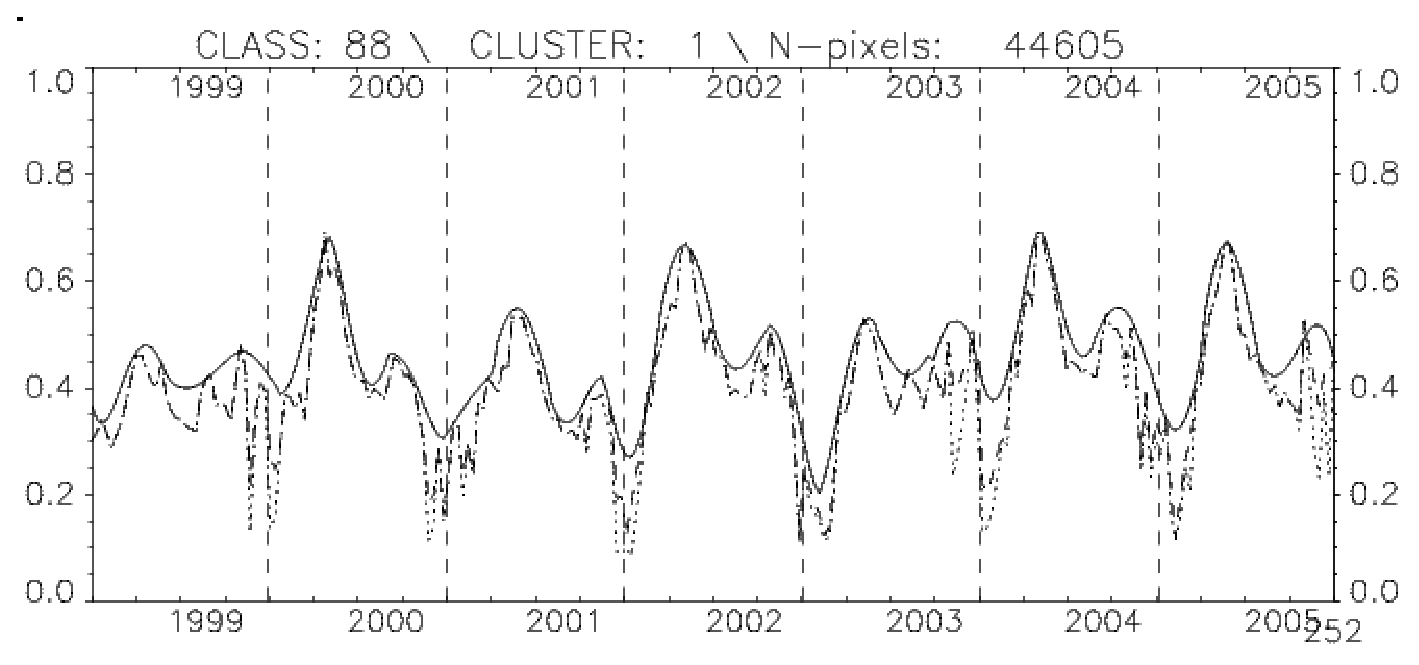
\includegraphics[scale=0.7]{EPS/plot.eps}
\caption{\label{figure1} Example of NDVI profiles: rough (dotted), masked (dashed), smoothed (solid). 
(A technical error led to NDVI values overestimated of 0.09 but it has no impact on classification which is relative). }
\end{center}
\end{figure}

In Ecoclimap-II, NDVI satellite data come from SPOT/VEGETATION\footnote{http://free.vgt.vito.be/, http://www.spot.vegetation.com}. 
They are decadal, at true 1-km resolution, that 
is to say that, contrary to AVHRR, one pixel signal is theorically not contaminated by pixels around. Data range from 1999, january to 2005, december.\\ 
They are delivered with a mask encoded on 8 bits: 2 bits represent the situations: clear sky, shadow, uncertain, cloud; 
1 bit for snow and ice, 
1 bit for the land sea mask, and the 4 last bits for the quality of the 4 satellite radiometric bands. This mask is applied in order to keep clear sky 
pixels for which the quality of bands B2 (red) and B3 (near infrared) is good. The land/sea/snow distinction is set by to the classification.\\ 
The plots of NDVI mean profiles for the covers of the C76 map show that data, even if cleared from aberrant values by the mask, remain noisy. 
That's why a smoothing is realized at the upper envelope of the rough curve because highest values are supposed better because atmospheric parameters 
(clouds, water vapor, aerosols) are likely to attenuate the signal reflected to the satellite. Anyway the work on NDVI time series is relative and 
the exact NDVI values don't matter. The smoothing is based on a 4-degree polynomial. 
The figure \ref{figure1} shows effects of the mask and smoothing on the mean NDVI signal for a given class. The distance between the rough and the 
smoothed curves is relative to this mean: the smoothing is done pixel by pixel, filtering out low values entering the mean in the rough case. 

\subsection{The automatic classification process}\label{classif}

The classification algorithm is \textbf{k-means}. 
It consists in reading the NDVI profiles of all pixels of one class, then of gathering closest profiles 
according to the Euclidian distance. Initial center-profiles of clusters are randomly defined and successive iterations are 
performed: each pixel is linked to the most like-looking center-profile; centers of clusters are recalculated; pixels are linked to 
the most like-looking center-profile again, and so on. It's thus necessary to fix from the beginning the number of wished clusters by class.\\ 
A first map is realized by setting high numbers of clusters by classes, then looking at NDVI profiles and geographic positions of the clusters, and 
setting new lower numbers of clusters, until a satisfying classification is obtained. This first map comprises 464 classes and is called \textbf{C464}. \\ 
However, for practical purposes, this method poses several problems: 
\begin{itemize}
\item{When each class of C76 is split into several clusters, the total number of classes increases very fast, rendering 
reading, interpretation and processing hard; }
\item{it boils down to consider initial classes as frozen and separated each from one another, what can prove false, notably with various 
initial maps;}
\item{the continuity of analysis is compromised and the quality of NDVI as classification criterion is hard to evaluate. Moreover, 
numbers of clusters have no option but being arbitrarily posed. }
\end{itemize}
Owing to all these reasons, NDVI is no longer used as a secondary classification criterion: it's admitted that it can rival the initial 
C76 classes boundaries. Moreover, three quantities are now taken into account during the NDVI classification:
\begin{itemize}
\item{the Euclidian distance between profiles (still);}
\item{the correlation between profiles, focusing on the shapes of profiles;}
\item{a criterion mixing the two precedents: $\frac{euclidian~distance}{correlation^{2}}$, outlining the shapes of profiles without neglecting 
the distance between them.}
\end{itemize}
The principle is to gather profiles using a threshold for one or the other of the latter criterions.
Other conditions come then into the picture:
\begin{itemize}  
\item{the size of classes: for example, the threshold is looser for smaller classes, in order not to encourage the formation of low pixels 
number classes;}
\item{the NDVI maximum: as NDVI is the expression of vegetation activity, it's not relevant with low-vegetated areas, also low NDVI maximum 
areas;}
\item{the cover type: water, town and bare soil pixels can't be distinguished through the NDVI, they have to conform the initial nomenclature.}
\end{itemize}
Lastly, comparisons are conducted:
\begin{itemize}
\item{between profiles of clusters and classes they come from: if the cluster is closer to another class than the one it comes from, it can be 
linked to the former class;}
\item{families of classes are formed, then splited in a number of clusters equal to the number of classes constituing them, through the 
automatic classification. Clusters obtained by this totally automatic means are compared to initial classes, in order to verify 
the robustness of the first method through it consistency with the second one. }
\end{itemize}
At each step, the geographic position, the contents of classes according to the initial nomenclature, NDVI profiles and standard deviations 
are observed. These operations allow a better approach of the NDVI time series, adapting to the different types of covers and ensuring more mixing and flexibility than if initial 
boudaries between classes were perfectly respected and if the strict k-means method was applied. 
At this point, the map under construction comprises 257 classes and is called \textbf{C257}. 

\subsection{To the resulting map}\label{end_map}

Several means are added to complete the new map realization:
\begin{itemize}
\item{C257 is compared with the map realized by purely respecting the classes boundaries, C464. 
Every class of each map is splited into 5 clusters through the automatic classification. The distance, the correlation and the standard 
deviation between each cluster and its mother-class are calculated. Maximum, minimum and median of these quantities are compared for C257 and 
C464. Results are equivalent whereas the total numbers of classes clearly vary between the two maps.}
\item{C257 is compared to C76. C76 covers are grouped into 14 general types, close to ISBA vegetation types. Then, each C257 class is divided 
in its contributions to the latter 14 types. Associated NDVI profiles are plotted; geographic distribution of so-obtained clusters is also 
examined. These operations aim at verifying that mixing of initial classes produce consistent and acceptable results. \\
First, given the high resemblance of NDVI profiles of some classes, pixels from a class corresponding to a type (among the 14) that is neither 
its first nor its second prevailing are moved to a class where the considered type prevails, provided that the resemblance between the two classes 
is sufficient (on NDVI profiles). The $\frac{distance}{correlation^{2}}$ criterion is used with a threshold: the moving occurs if the criterion 
is lower than 1., provided that the correlation is positive and higher than 0.9. This operation allows to considerably reduce the distance 
between C76 and C257 in terms of nomenclature. It's also verified that geographically gathered parts of land are not contradictory. Results 
are satisfying. Lastly, on a case by case basis, couple of last reshapings are done. The C257 map becomes at this point \textbf{C271} (with 271 classes). }
\item{NDVI profiles are plotted for only part of the pixels of classes. They are plotted for french pixels and on several specialized classes 
coming from CLC2000: vineyards, orchards, rice fields, olive groves. The goal is to check that those pixels, often melted in larger classes, 
haven't a very particular behaviour that would have been flooded during the classification. This process leads to add still 2 classes of 
vineyards. The final resulting map comprises 273 classes and is called \textbf{C273}. }
\end{itemize}
To conclude, the Ecoclimap-II map comprises 273 classes (see fig. \ref{figure2} for an illustration).  
The classification process combines both an automatic k-means algorithm on NDVI 
seven-years time series from SPOT/VGT and a more or less leaning constraint provided by an initial map built from existing land cover maps 
that are CLC2000 and GLC2000. The nomenclature of this map serves to contain the automatic classification and avoid the emergence of 
incoherent classes. \\
Note also that the use of seven-years time series data induces that the inter-annual variability is taken into account 
during the classification process. 


\begin{figure}
\begin{center}
\includegraphics[scale=0.4]{EPS/europe_eco2.eps}
\caption{\label{figure2} Ecoclimap-II C273 map on Europe (one color by class) (latlon projection)} 
\end{center}
\end{figure}

\subsection{Short description of covers}

To summarize, it can be said that:
\begin{itemize}
\item{Distribution of forests over the domain is quite linear and progressive, either on the geographic or on the NDVI profiles sides. The evolution 
follows a north-east to south-west axis.}
\item{Crops are very regionalized, in areas with well-marked outlines; they doesn't seem to follow a strictly natural logic. Indeed, 
the human intervention plays a role for these kinds of covers.}
\item{Distribution of shrubs and meadows is intermediate between forests and crops.}
\item{Concerning bare land, snow, inland water and urban areas, resulting classes are very close to those of the initial map C76. Indeed, the NDVI 
classification doesn't allow to discriminate such types of covers. However, the analysis of NDVI profiles is efficient to separate pure 
pixels from mixed ones, and to classify areas functions of the vegetation part of mixed ones. Nevertheless, maintaining such distinctions 
generates a very important amount of classes. That's why only few of these nuances are really integrated in C273, much with bare land and 
snow, just a little with inland water, not at all with urban areas. It could be interesting in the future to study the relevance of such 
distinctions.}
\end{itemize}
Generally, ecosystems are rather homogeneous on large areas in the north continental, and very mixed in the mediterranean perimeter. \\

For practical purposes, it can be noted that classes are numbered from 301 to 573; sea and oceans present in the European domain 
take the number 1 from Ecoclimap-I. 

\section{Translation of covers in tiles and vegetation types}

The next step is to define every new cover as a linear combination of the 4 tiles (types of surface) and the 12 vegetation types (inside 
the "nature" tile). The available sources are following:
\begin{itemize}
\item{(a) Nomenclatures at 1-km resolution from CLC2000, GLC2000 (world, Europe, North Eurasia, Asia, Africa), Ecoclimap-I, C76 (initial map for the classification, see \ref{init_map});}
\item{(a)' The nomenclature at 100m resolution from CLC2000;}
\item{(b) Agricultural statistics from Agreste on France, expressed in hectares, available department by department, since 1989. They comprise 
details about the types of crops;}
\item{(c) a global map about the distribution of C4 vegetation, at 1-degree resolution, provided within the framework of ISLSCP2 and dating from 2003;}
\item{(d) estimates of farm produce by european state, from the FAO;}
\item{(e) data on the maize production by european country in 2003, available on website Ma\"{i}sadour, in thousands of hectares.}
\end{itemize}
The method is then the following:
\begin{itemize}
\item{(a) each Ecoclimap-II cover is broken up among classes of considered other maps. Percentages of representation of the second in the first 
are listed and associated to the titles of the corresponding nomenclatures. The total percentage of the Ecoclimap-II cover in the considered 
map is indicated (in the case of Corine and GLC regional tiles, only a part of the domain is concerned). }
\item{(b) For AGRESTE, department by department, quantities of forests, meadows, C3 crops, C4 crops, permanent crops and other types of covers 
are calculated. Values are averaged on the 1999-2006 spell of time. Resulting curves are plotted and overlain with the associated Ecoclimap-II 
curves, functions of the way of repartition of the covers in the 12 vegetation types.}
\item{(c) The Ecoclimap-II C4 map is resampled at 1-degree resolution in order to compare with the ISLSCP2 map.}
\item{(d) (e) The FAO and Ma\"{i}sadour estimates haven't been exploited yet. }
\end{itemize}
If the class is included in the CORINE area at more than 50\%, the CORINE 100-m information is favoured, instead of 1-km nomenclatures. Amounts of 
C4, C3, meadows, forests, permanent crops are calibrated thanks to the AGRESTE curves, for well-represented classes on France. The ISLSCP2 
map allows to give an idea about the C4 distribution outside France. Note that Agreste provides informations on irrigated surfaces that 
haven't been exploited yet.


\section{Initialization of LAI profiles and other parameters}

In Ecoclimap, as seen in tab. \ref{tab4a} and tab. \ref{tab4b}, several parameters are initialized at the cover level. 

\subsection{Initialization of heights of trees, ground depths, irrigation and town parameters}

First of them, heights of trees are set by using Ecoclimap-I values and the compositions of Ecoclimap-II covers 
into other nomenclatures (GLC, CLC, Ecoclimap-I). Concerning shrubs classes, a distinction is done between meadows 
and low-level trees.\\ 
Then, the ground depths are set by using exclusively the Ecoclimap-I information, the only available. \\
These two last parameters would gain by benefiting from other sources of information.\\ 
Then, the vegetation type "irrigated crops" is arbitrarily considered as composed of C4 crops only. 
In Surfex, the modelling of irrigation passes by four parameters (cf tab. \ref{tab2a}): SEED, REAP, WATSUP and IRRIG. In Ecoclimap-I, 
by default these variables take constant values that are respectively: 10/05, 01/08, 30 and 1. In Ecoclimap-II, these 
default values are kept and defined as soon as the "irrigated crops" fraction is not null. It would be worth leaning on these values 
and precise them according to the classes. \\
Lastly, town parameters don't change in Ecoclimap-II: Ecoclimap urban 
classes are the same in the two versions and come directly from the CLC nomenclature. 

\subsection{Initialization of LAI}

The LAI (Leaf Area Index) is defined as the ratio of total upper leaf (or needle) 
surface of vegetation divided by the surface area of the land on which the vegetation grows. The effective LAI seen by the satellite 
is not the same as the in-situ LAI used by ISBA: the latter is measured on the whole thickness of the vegetation whereas the satellite 
sees only the top of canopy and deduces the LAI by more or less performing algorithms. It notably often causes saturations 
for high LAI. 

\subsubsection{LAI by cover}

Two satellite LAI have been examined for Ecoclimap-II: CYCLOPES (SPOT/VEGETATION) and MODIS. Algorithms leading from the satellite bands 
to the LAI are complex. Land cover maps are included, and the 7 satellite bands (in the case of SPOT) are used. CYCLOPES data range 
from 2000, January to 2004, December; MODIS data from 2000, March to 2006, December. As for the NDVI (see \ref{ndvi}), 
a smoothing by pixel at the 
upper envelop of the LAI profiles is performed. This smoothing is debatable because it makes average LAI values by class very higher 
than these of rough LAI. \\
MODIS LAI, CYCLOPES LAI and SPOT/VGT NDVI are plotted by cover so as to be compared. The three 
products are quite correlated, but MODIS LAI values tend to be higher on forests. Given that 
MODIS LAI time series are longer and that higher values on forests seem more realistic, MODIS LAI are kept 
for Ecoclimap-II. Nonetheless, preconceptions relative to the smoothing could lead in the future to review this LAI and its 
range of values in particular, all the more because tests of smoothing with varying parameters give clearly different results. \\
Moreover, there is a mask with MODIS data that distinguishes not classed data, built areas, wetlands and marshes, permanent 
snow, ice and tundra, bare soil or sparse vegetation areas, inland water, missing data. These masked values can be interpolated in the time 
series, excluded or replaced by zero during the smoothing. It happens that missing data are very numerous at the end of 2000 and 2001, 
particularly for northern and continental classes. That's why, finally, LAI times series are kept only from 2002, January, in order not 
to damage average on all years. It appears necessary to replace masked values because of snow, bare soil or water by zero, since 
LAI are otherwise not realistic (what is seen during the disaggregation coming next). On the contrary, missing and not classed values are interpolated 
in the limit of 4 successive decades, but those which are not interpolated are ignored during the calculation of means by cover 
(acceptable insofar as they are not predominant). 


\subsubsection{Disaggregation of LAI by vegtype inside covers}

\begin{table}[h]
\begin{center}
\begin{tabular}{|l|l|l|l|l|l|l|l|l|l|l|l|l|}
\hline
 & \multicolumn{10}{|c|}{\textbf{fraction of vegetation type}} \\
\hline
\textbf{vegtype} & 90-100\% &  80-90\% & 70-80\% & 60-70\% & 50-60\% & 40-50\% & 30-40\% & 20-30\% & 10-20\% & 0-10\% \\
\hline
CONI & 0 &  6  & 3  & 1  & 3  & 2  & 4  & 4 & 13 & 65 \\
\hline
TREE  & 0 &  2 &  0  & 0 &  1 &  2  & 3 &  6 & 26 & 60 \\
\hline
EVER  & 0  & 0  & 0 &  0  & 0  & 0  & 0 &  0 &  0 &  0 \\
\hline
GRAS  & 0 &  1 &  4 &  2  & 7 & 10 & 14 & 16 & 17 & 29 \\
\hline
TROG  & 0  & 0  & 0  & 0  & 0  & 0 &  0  & 0  & 0 & 100 \\
\hline
PARK  & 9 &  2 &  0 &  0 &  2 &  0 &  2 &  0  & 3 & 83 \\
\hline
C3  & 0  & 1 &  5  & 9  & 9  & 5  & 9 &  5 & 13 & 45 \\
\hline
C4  & 0 &  0 &  1 &  1 &  0 &  1 &  0 &  0 &  2 & 95 \\
\hline
IRR  & 0 &  3  & 5  & 3  & 0  & 2 &  3  & 2  & 2 & 81 \\
\hline
SNOW & 50 &  0 &  0 &  0  & 0 &  0  & 0 &  0 &  0 & 50 \\
\hline
NO  & 3  & 2 &  3 &  4 &  6 &  8 &  6 & 11 & 22 & 35 \\
\hline
ROCK  & 2  & 0  & 0 &  0  & 0 &  0  & 1 &  5  & 7 & 85 \\
\hline
total & 1  & 2 &  3  & 2 &  4 &  4 &  6 &  7 & 15 & 57 \\
\hline
\end{tabular}
\end{center}
\caption{Percentages of classes (calculated functions of the total numbers of classes by vegetation type) concerned by 
the fraction (columns) of each of the 12 vegetation types (lines)}
\label{tab10}
\end{table}

\begin{table}[h]
\begin{center}
\begin{tabular}{|l|l|l|l|l|l|l|l|l|l|}
\hline
\textbf{nb of vegtypes or tiles n} & 1 & 2 & 3 & 4 & 5 & 6 & 7 & 8 & 9 \\
 \hline
\textbf{nb of classes (vegtypes)} & 13  & 6  & 19 & 44 & 45 & 72 & 44 & 23 & 6 \\
\hline
\textbf{nb de classes (tiles)} & 126 & 94 & 53 & 0 & / &  / &  / &  / & / \\
\hline
\end{tabular}
\end{center}
\caption{Number of classes comprising n vegetation types (second line) or n tiles (third line)}
\label{tab11}
\end{table}


Remains to determine LAI by vegtype inside covers from LAI by cover. Given the complexity of classes in terms of vegetation types composition 
(see tab. \ref{tab10} and tab. \ref{tab11}), an automatic LAI disaggregation technique is welcome. The principle of the 
applied method is the following:
\begin{itemize}
\item{LAI 5-years profiles by cover are averaged in order to obtain the annual mean cycles.}
\item{LAI from vegetation types NO, ROCK and SNOW are supposed null and constant.}
\item{In each class, the main vegetation type is put apart. For each of the minority vegetation types, the LAI profile the closest 
according to the $\frac{distance}{correlation^{2}}$ criterion is searched, provided that it corresponds to a class where this vegetation type is 
majority. }
\item{The profile found is taken from the profile of the initial class, weighted by its representation fraction into the class.}
\item{One all minority vegetation types of the classes are thus processed, residual profiles of classes are obtained. Divided by 
the inverse of the fraction of the majority vegetation type, they are admitted to represent the pure majority profiles, in 
the classes.}
\item{The whole operation is repeated, replacing initial classes profiles by the previously obtained pure profiles.}
\item{A new set of pure profiles results, for majority vegetation types of classes. Plotting shows that the three profiles, initial 
(mixte), pure (first extimate), pure (second estimate) differ not much from one another. }
\item{Lastly, 5-years LAI profiles are built by propagating the error between years and the average on the obtained pure profiles.}
\end{itemize}
This method presents two problems: 
\begin{itemize}
\item{The seeking of approached classes only relies on profiles and not on the geographic localisation. Associations of classes coming 
from totally different climate areas are so expectable.}
\item{The technique of subtracting the secondary profiles to deduce the main profile might produce negative LAI.}
\end{itemize}
The first problem is corrected by introducing two climate maps (Firs on Europe, Koeppe et de Lond on the rest of the world). In the 
algorithm above, climate proximity is now favoured with the seeking beginning in the most represented climate area, next the second, etc. 
The second problem is solved by excluding a profile if its subtraction give negative values of LAI. If no suitable profile is found, this which gives 
the less negative values is linearly transformed in order to keep values just over zero. \\

This method presents the advantages that it relies only on the LAI profiles of covers, and doesn't create theoritical profiles. It's fast and 
supple (the longer step is to verify the spatial coherence of the origins of majority and minority profiles) and can be reprocessed 
in case of modifications of the distribution of classes among the 12 vegetation types. It ensures to diversify vegetation types profiles 
inside covers and guarantees the exact reconstitution of LAI covers profiles. However, it should be evaluated if the initial approximation 
between the cover profile and the main vegetation type profile doesn't produce too much bias in the definition of supposed pure profiles. 
But before, MODIS LAI also need to be validated.

\section{Study of the discontinuity at the limits of the domain}

For practical purposes, if the work area overflows the Ecoclimap-II domain, C273 is completed at its edges by Ecoclimap-I. First, north and major part 
of west of the 
domain, there is nearly only sea and ocean (apart from in New-Zemble, but the snow class Ecoclimap-II continues there in the snow class 
Ecoclimap-I). South and a little west, the boundary is located in the Sahara desert. Except from a possible discontinuity between bare rock and bare soil, 
and between very sparse vegetated and desert areas, 
the impact is so minor. Remains the East to study: from northern Russian tundra to Central Asia deserts, by Russian forests, it's 
about quite homogeneous areas organized with latitude, what already dulls the discontinuity.\\
Classes, LAI by class and by vegetation type and vegetation types fractions on both sides are compared. Ecoclimap-II 
classes generally continue in Ecoclimap-I classes. LAI and fractions are often different, but these discrepancies are rarely 
enormous. \\
It's so chosen to begin tests with the straight discontinuity. Then, if the delimitation is too obvious, 
it will be possible to contemplate a version with a smoothed (but artificial) delimitation. 

\chapter{Validation elements for Ecoclimap-II}

Validation aspects relate to three fields: 
\begin{itemize}
\item{Ecoclimap-II new map has already been quite examined during the processing, through comparisons with 
other existing land cover maps (GLC, CLC, Ecoclimap-I - see \ref{classif} and \ref{end_map}). Other tests could be performed, for 
example a comparison with GlobCover, a global land cover map for the year 2005-2006 using ENVISAT MERIS 
fine resolution (300m) data, developed by ESA (European Spatial Agency) and distributed by Medias-France.}
\item{Vegetation types fractions have been set in the light of existing land cover map nomenclatures. Other comparisons 
have been realized with AGRESTE and ISLSCP2 to calibrate values, but also a posteriori with Formosat on a square 
of 60km at the south-west of Toulouse, France. Formosat describes the land cover, year by year, on this area; 
the resolution is 20m. This map is produced by the CESBIO\footnote{Centre d'Etudes Spatiales de la 
BIOsphere (spatial study of the biosphere center)}. This last comparison gives encouraging results but also 
reveals the difficulty of different sources to agree: sources are sometimes contradictory, 
their charasterics and the geographic precision vary and are not necessarily easy to compare. However, 
the progressive use of more recent sources should allow to still refine this definition. Concerning 
specialized vegetation types thar are C4 crops, tropical grassland, irrigated crops, a lack of 
homogeneity inside the covers doesn't allow to get precise fractions. It could be interesting to 
make a potential new map with covers built by introducing entering informations about such characteristics. }
\item{Difficulties have been met to validate other parameters initialized at the cover level: heights of 
trees, ground depths, LAI profiles and irrigation parameters. Indeed, complete and reliable sources 
aren't available. A prospect for the following is thus to find means of validating these quantites. Note again that 
the organization by covers yields a constraint (especially for irrigation) whose reliance could also be interrogated in the light 
of such new validating data. }
\end{itemize}


\chapter{Conclusion}

Ecoclimap-II keeps the same general structure as Ecoclimap-I but several points have changed:
\begin{itemize}
\item{The new covers relie on a k-means automatic classification process and on recent existing land 
cover maps (GLC2000, CLC2000);}
\item{The vegetation types fractions and other cover-based parameters are consequently re-initialized, with 
help from several information sources (AGRESTE, ISLSCP2, land cover maps nomenclatures);}
\item{The LAI profiles by cover come from MODIS satellite data, they are smoothed pixel by pixel;}
\item{The LAI profiles by vegetation type inside covers are built through an original automatic disaggregation 
process in which only LAI profiles by cover step in; }
\item{LAI profiles are available for the average of 5 years (2002-2006) or for each of these years. }
\end{itemize}
Except from these discrepancies, other surface parameters are still likewise obtained. The geographic and 
by patch aggregation also remains. 
Several comparisons with other products have already been done but Ecoclimap-II now needs to be used in 
order to better qualify improvements and wastes in relation with the first version. Further evolution of the database 
is considered functions of users returns and of potential newly available validation data. 

%====================
\bibliography{surfex_scidoc}
%====================


\part{LAND SURFACE ANALYSIS}
\chapter{Surface Offline Data Assimilation}
\minitoc
%=========================
\bibliographystyle{plain}
%=========================

\section{Introduction}
SURFEX Offline Data Assimilation (SODA) is the first implementation of a unified assimilation in SURFEX. The present description is based on the offline version from SURFEX v.8. It is assumed that this version is currently running on your computer, if not, the first step is to install such version before trying to use the SODA scheme. SODA permits the land surface analysis of screen level parameters, soil moisture and vegetation. The screen level analysis relies on a two-dimensional Optimal Interpolation (2D-OI). The soil moisture and/or vegetation analysis rely either on a simplified Extended Kalman Filter or an Ensemble Kalman Filter (EnKF).

\section{Source code - creation of the binary}
SODA is available under the directory \$SURFEX\_EXPORT/src/ASSIM. Main file is {\bf soda.F90} that performs the various steps of the assimilation : definition of initial perturbed states, reading of fields from SURFEX outputs, writing of fields necessary for the analysis, and finally the surface analysis. The latter being executed by either {\bf assim\_nature\_isba\_oi.F90}, {\bf assim\_nature\_isba\_ekf.F90} or {\bf assim\_nature\_isba\_enkf.F90}.

\section{Optimal Interpolation soil moisture analysis}
{\large {\bf Methodology}} \\
This soil analysis scheme is based on an “local” optimum interpolation technique as described in Mahfouf (1991)\nocite{mahfouf_1991}, Giard and Bazile (2000)\nocite{giard_bazile_00}. The analysis increments from the screen-level analysis (2-meter temperature, $T_2m$ and relative humidity, $RH_2m$) are used to produce increments for the water content given by: \\
\begin{equation}
\Delta w_{s} = \alpha_s^T  \Delta T_{2m} + \alpha_s^{RH} \Delta RH_{2m}
\end{equation}
and
\begin{equation}
\Delta w_{p} = \alpha_p^T  \Delta T_{2m} + \alpha_p^{RH} \Delta RH_{2m}
\end{equation}

for the superficial volumetric and mean volumetric water content, respectively. The coefficients $\alpha_p^T$ and $\alpha_p^{RH}$ depend on soil texture, increasing as the standard range of variation of soil moisture $\delta w = \delta w_{fc} - \delta w_{wilt}$ (soil water content at field capacity and wilting point, respectively).

\section{Extended Kalman Filter soil moisture and vegetation analysis}
{\large {\bf Methodology}} \\
The EKF soil moisture analysis used in {\bf SODA} is a point wise data assimilation scheme (Mahfouf \etal (2009)\nocite{mahfouf_2009}, Barbu \etal (2011, 2014)\nocite{barbu_2011} \nocite{barbu_2014}, Fairbairn \etal (2017)\nocite{fairbairn_2017}, Albergel \etal (2017)\nocite{albergel_2017}). The analysis update equation of the EKF is: \\
\begin{equation}
x_a(t_i) = x_f(t_i)+K_i(y_0(t_i)-h_i[x_f])
\end{equation}

The $a$, $f$ and $o$ subscripts stand for analysis, forecast and observation, respectively. $x$ is the control vector of dimension $N_x$, computed at time $t_i$, that represents the prognostic equations of the LSM {\it $M$}.

$y_o$ is the observation vector of dimension $N_y$. The Kalman gain matrix $K_i$ is computed at time $t_i$ as: \\
\begin{equation} \label{eq2}
K_i = BH^T (HBH^T+R)^{-1}
\end{equation}

A non-linear observation operator $h$, enables the extraction of the model counterpart of the observations: \\
\begin{equation}
y(t_i) = h(x)
\end{equation}

$B$ and $R$ are error covariance matrices characterising the forecast and observations vectors. The cross-correlated terms represent covariances. The operator $H$ (and its transpose $H^T$) from \ref{eq2} is the Jacobian matrix: the linearized version of the observation operator (defined as $N_y$ rows and $N_x$ columns) that transforms the model states into the observations space. A numerical estimation of each Jacobian element is calculated by finite differences, by perturbing each component $x_j$ of the control vector $x$ by a specific amount $\delta x_j$ resulting in a column of the matrix $H$ for each integration $m$: 

\begin{equation}
H_{mj} = \frac{\partial {y}_m}{\partial {x}_j} \approx \frac{ {y}_m(x+\delta x_j)-y_m}{ \delta {x}_j}
\end{equation}

The background error covariance matrix undergoes an analogous forecast and analysis cycle:

\begin{equation} \label{eq5}
B_f(t_i) = M(t_{i-1}) B_a(t_{i-1}) M^T(t_{i-1}) + Q
\end{equation}

\begin{equation} \label{eq6}
B_a(t_i) = (I-K(t_i)H(t_i)) B_a(t_{i})
\end{equation}

In the forecast step (equation \ref{eq5}), the previous analysis, $B_a (t_{i-1})$, is forecast forward in time by the tangent linear of the state forecast model $M$, and the forecast error covariance matrix $Q$, is added to account for errors in the model forecast, giving the background error matrix forecast $B_f (t_i)$. The model state analysis decreases the model error, and $B$ is reduced by an analysis step (equation \ref{eq6}). The linearization of $M$ is obtained by the same finite difference method used for $H$.
The control vector evolution from time $t_i$ to time $t_{i+1}$ is then controlled by the following equation:


\begin{equation} \label{eq7}
x_f(t_{i+1}) = M_i[x_a(t_{i})]
\end{equation}

\section{Ensemble Kalman Filter soil moisture and vegetation analysis}

Although an EnKf analysis is available within SODA (Fairbairn \etal (2015)\nocite{fairbairn_2015}), it is still in consolidation phase.

%====================
\bibliography{surfex_scidoc}
%====================


%======================
%\bibliography{surfex_scidoc}
%======================

\end{document}
